\batchmode
\documentclass[a4paper]{book}
\usepackage{makeidx}
\usepackage{natbib}
\usepackage{graphicx}
\usepackage{multicol}
\usepackage{float}
\usepackage{listings}
\usepackage{color}
\usepackage{ifthen}
\usepackage[table]{xcolor}
\usepackage{textcomp}
\usepackage{alltt}
\usepackage[utf8]{inputenc}
\usepackage{mathptmx}
\usepackage[scaled=.90]{helvet}
\usepackage{courier}
\usepackage{sectsty}
\usepackage[titles]{tocloft}
\usepackage{doxygen}
\lstset{language=C++,inputencoding=utf8,basicstyle=\footnotesize,breaklines=true,breakatwhitespace=true,tabsize=8,numbers=left }
\makeindex
\setcounter{tocdepth}{3}
\renewcommand{\footrulewidth}{0.4pt}
\renewcommand{\familydefault}{\sfdefault}
\hfuzz=15pt
\setlength{\emergencystretch}{15pt}
\hbadness=750
\tolerance=750
\begin{document}
\begin{titlepage}
\vspace*{7cm}
\begin{center}
{\Large oryx\-\_\-path\-\_\-planning }\\
\vspace*{1cm}
{\large \-Generated by Doxygen 1.7.6.1}\\
\vspace*{0.5cm}
{\small Sun Jan 20 2013 12:23:01}\\
\end{center}
\end{titlepage}
\clearemptydoublepage
\pagenumbering{roman}
\tableofcontents
\clearemptydoublepage
\pagenumbering{arabic}
\chapter{\-Main \-Page}
\label{index}

{\bfseries \doxyref{oryxsrr\-\_\-msgs}{p.}{namespaceoryxsrr__msgs}} 

-\/-\/$>$ 
\chapter{\-Todo \-List}
\label{todo}

\begin{DoxyRefList}
\item[\label{todo__todo000001}%
\-Member \doxyref{oryx\-\_\-path\-\_\-planning\-:\-:\-Occupancy\-Grid\-:\-:generate\-Message}{p.}{classoryx__path__planning_1_1OccupancyGrid_a28709bca2d63cf5951fc1d9de0c1f11f} (sensor\-\_\-msgs\-::\-Image \&message) const ]\-Currently, it assumes a 2\-D, \-X\-Y grid. \-Will still work with 3\-D, but will only take the \-X\-Y plane at \-Z=0 
\end{DoxyRefList}
\chapter{\-Namespace \-Index}
\section{\-Namespace \-List}
\-Here is a list of all namespaces with brief descriptions\-:\begin{DoxyCompactList}
\item\contentsline{section}{{\bf \-Translate\-Control\-Server} }{\pageref{namespaceTranslateControlServer}}{}
\end{DoxyCompactList}

\chapter{\-Class \-Index}
\section{\-Class \-Hierarchy}
\-This inheritance list is sorted roughly, but not completely, alphabetically\-:\begin{DoxyCompactList}
\item \contentsline{section}{oryx\-\_\-path\-\_\-planning\-:\-:\-Chainable\-Exception}{\pageref{classoryx__path__planning_1_1ChainableException}}{}
\begin{DoxyCompactList}
\item \contentsline{section}{oryx\-\_\-path\-\_\-planning\-:\-:\-Occupancy\-Grid\-Access\-Exception}{\pageref{classoryx__path__planning_1_1OccupancyGridAccessException}}{}
\item \contentsline{section}{oryx\-\_\-path\-\_\-planning\-:\-:\-Speed\-Set\-Access\-Exception}{\pageref{classoryx__path__planning_1_1SpeedSetAccessException}}{}
\item \contentsline{section}{oryx\-\_\-path\-\_\-planning\-:\-:\-Tentacle\-Access\-Exception}{\pageref{classoryx__path__planning_1_1TentacleAccessException}}{}
\item \contentsline{section}{oryx\-\_\-path\-\_\-planning\-:\-:\-Tentacle\-Generation\-Exception}{\pageref{classoryx__path__planning_1_1TentacleGenerationException}}{}
\end{DoxyCompactList}
\item \contentsline{section}{\-Command\-Engine}{\pageref{classCommandEngine}}{}
\item \contentsline{section}{oryx\-\_\-path\-\_\-planning\-:\-:constants}{\pageref{classoryx__path__planning_1_1constants}}{}
\item \contentsline{section}{ros\-:\-:message\-\_\-traits\-:\-:\-Data\-Type$<$ \-:\-:oryx\-\_\-path\-\_\-planning\-:\-:\-Occupancy\-Grid\-\_\-$<$ \-Container\-Allocator $>$ $>$}{\pageref{structros_1_1message__traits_1_1DataType_3_01_1_1oryx__path__planning_1_1OccupancyGrid___3_01ContainerAllocator_01_4_01_4}}{}
\item \contentsline{section}{ros\-:\-:message\-\_\-traits\-:\-:\-Data\-Type$<$ \-:\-:oryx\-\_\-path\-\_\-planning\-:\-:\-Occupancy\-Grid\-Msg\-\_\-$<$ \-Container\-Allocator $>$ $>$}{\pageref{structros_1_1message__traits_1_1DataType_3_01_1_1oryx__path__planning_1_1OccupancyGridMsg___3_01ContainerAllocator_01_4_01_4}}{}
\item \contentsline{section}{ros\-:\-:message\-\_\-traits\-:\-:\-Definition$<$ \-:\-:oryx\-\_\-path\-\_\-planning\-:\-:\-Occupancy\-Grid\-\_\-$<$ \-Container\-Allocator $>$ $>$}{\pageref{structros_1_1message__traits_1_1Definition_3_01_1_1oryx__path__planning_1_1OccupancyGrid___3_01ContainerAllocator_01_4_01_4}}{}
\item \contentsline{section}{ros\-:\-:message\-\_\-traits\-:\-:\-Definition$<$ \-:\-:oryx\-\_\-path\-\_\-planning\-:\-:\-Occupancy\-Grid\-Msg\-\_\-$<$ \-Container\-Allocator $>$ $>$}{\pageref{structros_1_1message__traits_1_1Definition_3_01_1_1oryx__path__planning_1_1OccupancyGridMsg___3_01ContainerAllocator_01_4_01_4}}{}
\item \contentsline{section}{ros\-:\-:message\-\_\-traits\-:\-:\-Has\-Header$<$ \-:\-:oryx\-\_\-path\-\_\-planning\-:\-:\-Occupancy\-Grid\-\_\-$<$ \-Container\-Allocator $>$ $>$}{\pageref{structros_1_1message__traits_1_1HasHeader_3_01_1_1oryx__path__planning_1_1OccupancyGrid___3_01ContainerAllocator_01_4_01_4}}{}
\item \contentsline{section}{ros\-:\-:message\-\_\-traits\-:\-:\-Has\-Header$<$ \-:\-:oryx\-\_\-path\-\_\-planning\-:\-:\-Occupancy\-Grid\-Msg\-\_\-$<$ \-Container\-Allocator $>$ $>$}{\pageref{structros_1_1message__traits_1_1HasHeader_3_01_1_1oryx__path__planning_1_1OccupancyGridMsg___3_01ContainerAllocator_01_4_01_4}}{}
\item \contentsline{section}{ros\-:\-:message\-\_\-traits\-:\-:\-Has\-Header$<$ const \-:\-:oryx\-\_\-path\-\_\-planning\-:\-:\-Occupancy\-Grid\-\_\-$<$ \-Container\-Allocator $>$ $>$}{\pageref{structros_1_1message__traits_1_1HasHeader_3_01const_01_1_1oryx__path__planning_1_1OccupancyGrid_92926d5829d603cda857668ddfe92ade}}{}
\item \contentsline{section}{ros\-:\-:message\-\_\-traits\-:\-:\-Has\-Header$<$ const \-:\-:oryx\-\_\-path\-\_\-planning\-:\-:\-Occupancy\-Grid\-Msg\-\_\-$<$ \-Container\-Allocator $>$ $>$}{\pageref{structros_1_1message__traits_1_1HasHeader_3_01const_01_1_1oryx__path__planning_1_1OccupancyGridM8f11ff1dc81e090e9a5769827c915e8c}}{}
\item \contentsline{section}{ros\-:\-:message\-\_\-traits\-:\-:\-Is\-Message$<$ \-:\-:oryx\-\_\-path\-\_\-planning\-:\-:\-Occupancy\-Grid\-\_\-$<$ \-Container\-Allocator $>$ $>$}{\pageref{structros_1_1message__traits_1_1IsMessage_3_01_1_1oryx__path__planning_1_1OccupancyGrid___3_01ContainerAllocator_01_4_01_4}}{}
\item \contentsline{section}{ros\-:\-:message\-\_\-traits\-:\-:\-Is\-Message$<$ \-:\-:oryx\-\_\-path\-\_\-planning\-:\-:\-Occupancy\-Grid\-\_\-$<$ \-Container\-Allocator $>$const $>$}{\pageref{structros_1_1message__traits_1_1IsMessage_3_01_1_1oryx__path__planning_1_1OccupancyGrid___3_01Coa7ac41d9ab8ac5873aa24172bd39fb77}}{}
\item \contentsline{section}{ros\-:\-:message\-\_\-traits\-:\-:\-Is\-Message$<$ \-:\-:oryx\-\_\-path\-\_\-planning\-:\-:\-Occupancy\-Grid\-Msg\-\_\-$<$ \-Container\-Allocator $>$ $>$}{\pageref{structros_1_1message__traits_1_1IsMessage_3_01_1_1oryx__path__planning_1_1OccupancyGridMsg___3_01ContainerAllocator_01_4_01_4}}{}
\item \contentsline{section}{ros\-:\-:message\-\_\-traits\-:\-:\-Is\-Message$<$ \-:\-:oryx\-\_\-path\-\_\-planning\-:\-:\-Occupancy\-Grid\-Msg\-\_\-$<$ \-Container\-Allocator $>$const $>$}{\pageref{structros_1_1message__traits_1_1IsMessage_3_01_1_1oryx__path__planning_1_1OccupancyGridMsg___3_066b071b372c64b6f41543f75cce14c40}}{}
\item \contentsline{section}{\-Local\-Planner}{\pageref{classLocalPlanner}}{}
\item \contentsline{section}{ros\-:\-:message\-\_\-traits\-:\-:\-M\-D5\-Sum$<$ \-:\-:oryx\-\_\-path\-\_\-planning\-:\-:\-Occupancy\-Grid\-\_\-$<$ \-Container\-Allocator $>$ $>$}{\pageref{structros_1_1message__traits_1_1MD5Sum_3_01_1_1oryx__path__planning_1_1OccupancyGrid___3_01ContainerAllocator_01_4_01_4}}{}
\item \contentsline{section}{ros\-:\-:message\-\_\-traits\-:\-:\-M\-D5\-Sum$<$ \-:\-:oryx\-\_\-path\-\_\-planning\-:\-:\-Occupancy\-Grid\-Msg\-\_\-$<$ \-Container\-Allocator $>$ $>$}{\pageref{structros_1_1message__traits_1_1MD5Sum_3_01_1_1oryx__path__planning_1_1OccupancyGridMsg___3_01ContainerAllocator_01_4_01_4}}{}
\item \contentsline{section}{oryx\-\_\-path\-\_\-planning\-:\-:\-Occupancy\-Grid}{\pageref{classoryx__path__planning_1_1OccupancyGrid}}{}
\item \contentsline{section}{oryx\-\_\-path\-\_\-planning.\-msg.\-\_\-\-Occupancy\-Grid.\-Occupancy\-Grid}{\pageref{classoryx__path__planning_1_1msg_1_1__OccupancyGrid_1_1OccupancyGrid}}{}
\item \contentsline{section}{oryx\-\_\-path\-\_\-planning\-:\-:\-Occupancy\-Grid\-\_\-$<$ \-Container\-Allocator $>$}{\pageref{structoryx__path__planning_1_1OccupancyGrid__}}{}
\item \contentsline{section}{oryx\-\_\-path\-\_\-planning.\-msg.\-\_\-\-Occupancy\-Grid\-Msg.\-Occupancy\-Grid\-Msg}{\pageref{classoryx__path__planning_1_1msg_1_1__OccupancyGridMsg_1_1OccupancyGridMsg}}{}
\item \contentsline{section}{oryx\-\_\-path\-\_\-planning\-:\-:\-Occupancy\-Grid\-Msg\-\_\-$<$ \-Container\-Allocator $>$}{\pageref{structoryx__path__planning_1_1OccupancyGridMsg__}}{}
\item \contentsline{section}{oryx\-\_\-path\-\_\-planning\-:\-:\-Point\-Converter}{\pageref{classoryx__path__planning_1_1PointConverter}}{}
\item \contentsline{section}{ros\-:\-:message\-\_\-operations\-:\-:\-Printer$<$ \-:\-:oryx\-\_\-path\-\_\-planning\-:\-:\-Occupancy\-Grid\-\_\-$<$ \-Container\-Allocator $>$ $>$}{\pageref{structros_1_1message__operations_1_1Printer_3_01_1_1oryx__path__planning_1_1OccupancyGrid___3_01ContainerAllocator_01_4_01_4}}{}
\item \contentsline{section}{ros\-:\-:message\-\_\-operations\-:\-:\-Printer$<$ \-:\-:oryx\-\_\-path\-\_\-planning\-:\-:\-Occupancy\-Grid\-Msg\-\_\-$<$ \-Container\-Allocator $>$ $>$}{\pageref{structros_1_1message__operations_1_1Printer_3_01_1_1oryx__path__planning_1_1OccupancyGridMsg___3_01ContainerAllocator_01_4_01_4}}{}
\item \contentsline{section}{ros\-:\-:serialization\-:\-:\-Serializer$<$ \-:\-:oryx\-\_\-path\-\_\-planning\-:\-:\-Occupancy\-Grid\-\_\-$<$ \-Container\-Allocator $>$ $>$}{\pageref{structros_1_1serialization_1_1Serializer_3_01_1_1oryx__path__planning_1_1OccupancyGrid___3_01ContainerAllocator_01_4_01_4}}{}
\item \contentsline{section}{ros\-:\-:serialization\-:\-:\-Serializer$<$ \-:\-:oryx\-\_\-path\-\_\-planning\-:\-:\-Occupancy\-Grid\-Msg\-\_\-$<$ \-Container\-Allocator $>$ $>$}{\pageref{structros_1_1serialization_1_1Serializer_3_01_1_1oryx__path__planning_1_1OccupancyGridMsg___3_01ContainerAllocator_01_4_01_4}}{}
\item \contentsline{section}{oryx\-\_\-path\-\_\-planning\-:\-:\-Speed\-Set}{\pageref{classoryx__path__planning_1_1SpeedSet}}{}
\item \contentsline{section}{oryx\-\_\-path\-\_\-planning\-:\-:\-Tentacle}{\pageref{classoryx__path__planning_1_1Tentacle}}{}
\item \contentsline{section}{oryx\-\_\-path\-\_\-planning\-:\-:\-Tentacle\-Generator}{\pageref{classoryx__path__planning_1_1TentacleGenerator}}{}
\item \contentsline{section}{oryx\-\_\-path\-\_\-planning\-:\-:\-Tentacle\-:\-:\-Tentacle\-Traverser}{\pageref{classoryx__path__planning_1_1Tentacle_1_1TentacleTraverser}}{}
\end{DoxyCompactList}

\chapter{\-Class \-Index}
\section{\-Class \-List}
\-Here are the classes, structs, unions and interfaces with brief descriptions\-:\begin{DoxyCompactList}
\item\contentsline{section}{{\bf oryx\-\_\-srr\-\_\-gui\-::\-Main\-Window} \\*\-Qt central, all operations relating to the view part here }{\pageref{classoryx__srr__gui_1_1MainWindow}}{}
\item\contentsline{section}{{\bf oryx\-\_\-srr\-\_\-gui\-::\-Q\-Node} }{\pageref{classoryx__srr__gui_1_1QNode}}{}
\end{DoxyCompactList}

\chapter{\-File \-Index}
\section{\-File \-List}
\-Here is a list of all files with brief descriptions\-:\begin{DoxyCompactList}
\item\contentsline{section}{{\bf main.\-cpp} \\*\-Qt based gui }{\pageref{main_8cpp}}{}
\item\contentsline{section}{{\bf main\-\_\-window.\-cpp} \\*\-Implementation for the qt gui }{\pageref{main__window_8cpp}}{}
\item\contentsline{section}{{\bf main\-\_\-window.\-hpp} \\*\-Qt based gui for \doxyref{oryx\-\_\-srr\-\_\-gui}{p.}{namespaceoryx__srr__gui} }{\pageref{main__window_8hpp}}{}
\item\contentsline{section}{{\bf qnode.\-cpp} \\*\-Ros communication central! }{\pageref{qnode_8cpp}}{}
\item\contentsline{section}{{\bf qnode.\-hpp} \\*\-Communications central! }{\pageref{qnode_8hpp}}{}
\end{DoxyCompactList}

\chapter{\-Namespace \-Documentation}
\section{05 \-Namespace \-Reference}
\label{namespace05}\index{05@{05}}
\subsection*{\-Variables}
\begin{DoxyCompactItemize}
\item 
{\bf \-B\-U\-I\-L\-D\-S\-P\-A\-C\-E} = \-True
\item 
string {\bf \-C\-A\-T\-K\-I\-N\-\_\-\-B\-U\-I\-L\-D\-\_\-\-P\-R\-E\-F\-I\-X} = '/home/parallels/groovy\-\_\-workspace/oryx\-\_\-srr/oryx\-\_\-path\-\_\-planning/devel'
\item 
string {\bf \-C\-A\-T\-K\-I\-N\-\_\-\-D\-E\-V\-E\-L\-\_\-\-P\-R\-E\-F\-I\-X} = '/home/parallels/groovy\-\_\-workspace/oryx\-\_\-srr/oryx\-\_\-path\-\_\-planning/devel'
\item 
string {\bf \-C\-A\-T\-K\-I\-N\-\_\-\-G\-L\-O\-B\-A\-L\-\_\-\-B\-I\-N\-\_\-\-D\-E\-S\-T\-I\-N\-A\-T\-I\-O\-N} = 'bin'
\item 
string {\bf \-C\-A\-T\-K\-I\-N\-\_\-\-G\-L\-O\-B\-A\-L\-\_\-\-E\-T\-C\-\_\-\-D\-E\-S\-T\-I\-N\-A\-T\-I\-O\-N} = 'etc'
\item 
string {\bf \-C\-A\-T\-K\-I\-N\-\_\-\-G\-L\-O\-B\-A\-L\-\_\-\-I\-N\-C\-L\-U\-D\-E\-\_\-\-D\-E\-S\-T\-I\-N\-A\-T\-I\-O\-N} = 'include'
\item 
string {\bf \-C\-A\-T\-K\-I\-N\-\_\-\-G\-L\-O\-B\-A\-L\-\_\-\-L\-I\-B\-\_\-\-D\-E\-S\-T\-I\-N\-A\-T\-I\-O\-N} = 'lib'
\item 
string {\bf \-C\-A\-T\-K\-I\-N\-\_\-\-G\-L\-O\-B\-A\-L\-\_\-\-L\-I\-B\-E\-X\-E\-C\-\_\-\-D\-E\-S\-T\-I\-N\-A\-T\-I\-O\-N} = 'lib'
\item 
string {\bf \-C\-A\-T\-K\-I\-N\-\_\-\-G\-L\-O\-B\-A\-L\-\_\-\-P\-Y\-T\-H\-O\-N\-\_\-\-D\-E\-S\-T\-I\-N\-A\-T\-I\-O\-N} = 'lib/python2.\-7/dist-\/packages'
\item 
string {\bf \-C\-A\-T\-K\-I\-N\-\_\-\-G\-L\-O\-B\-A\-L\-\_\-\-S\-H\-A\-R\-E\-\_\-\-D\-E\-S\-T\-I\-N\-A\-T\-I\-O\-N} = 'share'
\item 
string {\bf \-C\-A\-T\-K\-I\-N\-\_\-\-P\-A\-C\-K\-A\-G\-E\-\_\-\-B\-I\-N\-\_\-\-D\-E\-S\-T\-I\-N\-A\-T\-I\-O\-N} = ''
\item 
string {\bf \-C\-A\-T\-K\-I\-N\-\_\-\-P\-A\-C\-K\-A\-G\-E\-\_\-\-E\-T\-C\-\_\-\-D\-E\-S\-T\-I\-N\-A\-T\-I\-O\-N} = ''
\item 
string {\bf \-C\-A\-T\-K\-I\-N\-\_\-\-P\-A\-C\-K\-A\-G\-E\-\_\-\-I\-N\-C\-L\-U\-D\-E\-\_\-\-D\-E\-S\-T\-I\-N\-A\-T\-I\-O\-N} = ''
\item 
string {\bf \-C\-A\-T\-K\-I\-N\-\_\-\-P\-A\-C\-K\-A\-G\-E\-\_\-\-L\-I\-B\-\_\-\-D\-E\-S\-T\-I\-N\-A\-T\-I\-O\-N} = ''
\item 
string {\bf \-C\-A\-T\-K\-I\-N\-\_\-\-P\-A\-C\-K\-A\-G\-E\-\_\-\-L\-I\-B\-E\-X\-E\-C\-\_\-\-D\-E\-S\-T\-I\-N\-A\-T\-I\-O\-N} = ''
\item 
string {\bf \-C\-A\-T\-K\-I\-N\-\_\-\-P\-A\-C\-K\-A\-G\-E\-\_\-\-P\-Y\-T\-H\-O\-N\-\_\-\-D\-E\-S\-T\-I\-N\-A\-T\-I\-O\-N} = ''
\item 
string {\bf \-C\-A\-T\-K\-I\-N\-\_\-\-P\-A\-C\-K\-A\-G\-E\-\_\-\-S\-H\-A\-R\-E\-\_\-\-D\-E\-S\-T\-I\-N\-A\-T\-I\-O\-N} = ''
\item 
string {\bf \-C\-M\-A\-K\-E\-\_\-\-B\-I\-N\-A\-R\-Y\-\_\-\-D\-I\-R} = '/home/parallels/groovy\-\_\-workspace/oryx\-\_\-srr/oryx\-\_\-path\-\_\-planning'
\item 
string {\bf \-C\-M\-A\-K\-E\-\_\-\-C\-U\-R\-R\-E\-N\-T\-\_\-\-B\-I\-N\-A\-R\-Y\-\_\-\-D\-I\-R} = '/home/parallels/groovy\-\_\-workspace/oryx\-\_\-srr/oryx\-\_\-path\-\_\-planning'
\item 
string {\bf \-C\-M\-A\-K\-E\-\_\-\-C\-U\-R\-R\-E\-N\-T\-\_\-\-S\-O\-U\-R\-C\-E\-\_\-\-D\-I\-R} = '/home/parallels/groovy\-\_\-workspace/oryx\-\_\-srr/oryx\-\_\-path\-\_\-planning'
\item 
string {\bf \-C\-M\-A\-K\-E\-\_\-\-I\-N\-S\-T\-A\-L\-L\-\_\-\-P\-R\-E\-F\-I\-X} = '/usr/local'
\item 
string {\bf \-C\-M\-A\-K\-E\-\_\-\-S\-O\-U\-R\-C\-E\-\_\-\-D\-I\-R} = '/home/parallels/groovy\-\_\-workspace/oryx\-\_\-srr/oryx\-\_\-path\-\_\-planning'
\item 
{\bf \-D\-E\-V\-E\-L\-S\-P\-A\-C\-E} = \-True
\item 
{\bf \-I\-N\-S\-T\-A\-L\-L\-S\-P\-A\-C\-E} = \-False
\item 
string {\bf \-P\-R\-O\-J\-E\-C\-T\-\_\-\-B\-I\-N\-A\-R\-Y\-\_\-\-D\-I\-R} = '/home/parallels/groovy\-\_\-workspace/oryx\-\_\-srr/oryx\-\_\-path\-\_\-planning'
\item 
string {\bf \-P\-R\-O\-J\-E\-C\-T\-\_\-\-N\-A\-M\-E} = 'oryx\-\_\-path\-\_\-planning'
\item 
string {\bf \-P\-R\-O\-J\-E\-C\-T\-\_\-\-S\-O\-U\-R\-C\-E\-\_\-\-D\-I\-R} = '/home/parallels/groovy\-\_\-workspace/oryx\-\_\-srr/oryx\-\_\-path\-\_\-planning'
\end{DoxyCompactItemize}


\subsection{\-Variable \-Documentation}
\index{05@{05}!\-B\-U\-I\-L\-D\-S\-P\-A\-C\-E@{\-B\-U\-I\-L\-D\-S\-P\-A\-C\-E}}
\index{\-B\-U\-I\-L\-D\-S\-P\-A\-C\-E@{\-B\-U\-I\-L\-D\-S\-P\-A\-C\-E}!05@{05}}
\subsubsection[{\-B\-U\-I\-L\-D\-S\-P\-A\-C\-E}]{\setlength{\rightskip}{0pt plus 5cm}05\-::{\bf \-B\-U\-I\-L\-D\-S\-P\-A\-C\-E} = \-True}\label{namespace05_a6843fe1cdad583aa5b47b9269a3cb1f9}


\-Definition at line 1 of file 05.\-catkin-\/test-\/results.\-sh.\-develspace.\-context.\-py.

\index{05@{05}!\-C\-A\-T\-K\-I\-N\-\_\-\-B\-U\-I\-L\-D\-\_\-\-P\-R\-E\-F\-I\-X@{\-C\-A\-T\-K\-I\-N\-\_\-\-B\-U\-I\-L\-D\-\_\-\-P\-R\-E\-F\-I\-X}}
\index{\-C\-A\-T\-K\-I\-N\-\_\-\-B\-U\-I\-L\-D\-\_\-\-P\-R\-E\-F\-I\-X@{\-C\-A\-T\-K\-I\-N\-\_\-\-B\-U\-I\-L\-D\-\_\-\-P\-R\-E\-F\-I\-X}!05@{05}}
\subsubsection[{\-C\-A\-T\-K\-I\-N\-\_\-\-B\-U\-I\-L\-D\-\_\-\-P\-R\-E\-F\-I\-X}]{\setlength{\rightskip}{0pt plus 5cm}string 05\-::{\bf \-C\-A\-T\-K\-I\-N\-\_\-\-B\-U\-I\-L\-D\-\_\-\-P\-R\-E\-F\-I\-X} = '/home/parallels/groovy\-\_\-workspace/oryx\-\_\-srr/oryx\-\_\-path\-\_\-planning/devel'}\label{namespace05_a7c9e5bee0b35d2901854f376fb3bc282}


\-Definition at line 5 of file 05.\-catkin-\/test-\/results.\-sh.\-develspace.\-context.\-py.

\index{05@{05}!\-C\-A\-T\-K\-I\-N\-\_\-\-D\-E\-V\-E\-L\-\_\-\-P\-R\-E\-F\-I\-X@{\-C\-A\-T\-K\-I\-N\-\_\-\-D\-E\-V\-E\-L\-\_\-\-P\-R\-E\-F\-I\-X}}
\index{\-C\-A\-T\-K\-I\-N\-\_\-\-D\-E\-V\-E\-L\-\_\-\-P\-R\-E\-F\-I\-X@{\-C\-A\-T\-K\-I\-N\-\_\-\-D\-E\-V\-E\-L\-\_\-\-P\-R\-E\-F\-I\-X}!05@{05}}
\subsubsection[{\-C\-A\-T\-K\-I\-N\-\_\-\-D\-E\-V\-E\-L\-\_\-\-P\-R\-E\-F\-I\-X}]{\setlength{\rightskip}{0pt plus 5cm}string 05\-::{\bf \-C\-A\-T\-K\-I\-N\-\_\-\-D\-E\-V\-E\-L\-\_\-\-P\-R\-E\-F\-I\-X} = '/home/parallels/groovy\-\_\-workspace/oryx\-\_\-srr/oryx\-\_\-path\-\_\-planning/devel'}\label{namespace05_a39137f4dcd97abcca937ef29e60694f5}


\-Definition at line 6 of file 05.\-catkin-\/test-\/results.\-sh.\-develspace.\-context.\-py.

\index{05@{05}!\-C\-A\-T\-K\-I\-N\-\_\-\-G\-L\-O\-B\-A\-L\-\_\-\-B\-I\-N\-\_\-\-D\-E\-S\-T\-I\-N\-A\-T\-I\-O\-N@{\-C\-A\-T\-K\-I\-N\-\_\-\-G\-L\-O\-B\-A\-L\-\_\-\-B\-I\-N\-\_\-\-D\-E\-S\-T\-I\-N\-A\-T\-I\-O\-N}}
\index{\-C\-A\-T\-K\-I\-N\-\_\-\-G\-L\-O\-B\-A\-L\-\_\-\-B\-I\-N\-\_\-\-D\-E\-S\-T\-I\-N\-A\-T\-I\-O\-N@{\-C\-A\-T\-K\-I\-N\-\_\-\-G\-L\-O\-B\-A\-L\-\_\-\-B\-I\-N\-\_\-\-D\-E\-S\-T\-I\-N\-A\-T\-I\-O\-N}!05@{05}}
\subsubsection[{\-C\-A\-T\-K\-I\-N\-\_\-\-G\-L\-O\-B\-A\-L\-\_\-\-B\-I\-N\-\_\-\-D\-E\-S\-T\-I\-N\-A\-T\-I\-O\-N}]{\setlength{\rightskip}{0pt plus 5cm}string 05\-::{\bf \-C\-A\-T\-K\-I\-N\-\_\-\-G\-L\-O\-B\-A\-L\-\_\-\-B\-I\-N\-\_\-\-D\-E\-S\-T\-I\-N\-A\-T\-I\-O\-N} = 'bin'}\label{namespace05_a6abb5037b1f0e558cb50e006a7319bb9}


\-Definition at line 8 of file 05.\-catkin-\/test-\/results.\-sh.\-develspace.\-context.\-py.

\index{05@{05}!\-C\-A\-T\-K\-I\-N\-\_\-\-G\-L\-O\-B\-A\-L\-\_\-\-E\-T\-C\-\_\-\-D\-E\-S\-T\-I\-N\-A\-T\-I\-O\-N@{\-C\-A\-T\-K\-I\-N\-\_\-\-G\-L\-O\-B\-A\-L\-\_\-\-E\-T\-C\-\_\-\-D\-E\-S\-T\-I\-N\-A\-T\-I\-O\-N}}
\index{\-C\-A\-T\-K\-I\-N\-\_\-\-G\-L\-O\-B\-A\-L\-\_\-\-E\-T\-C\-\_\-\-D\-E\-S\-T\-I\-N\-A\-T\-I\-O\-N@{\-C\-A\-T\-K\-I\-N\-\_\-\-G\-L\-O\-B\-A\-L\-\_\-\-E\-T\-C\-\_\-\-D\-E\-S\-T\-I\-N\-A\-T\-I\-O\-N}!05@{05}}
\subsubsection[{\-C\-A\-T\-K\-I\-N\-\_\-\-G\-L\-O\-B\-A\-L\-\_\-\-E\-T\-C\-\_\-\-D\-E\-S\-T\-I\-N\-A\-T\-I\-O\-N}]{\setlength{\rightskip}{0pt plus 5cm}string 05\-::{\bf \-C\-A\-T\-K\-I\-N\-\_\-\-G\-L\-O\-B\-A\-L\-\_\-\-E\-T\-C\-\_\-\-D\-E\-S\-T\-I\-N\-A\-T\-I\-O\-N} = 'etc'}\label{namespace05_a6f489a43ae250789dd71b9e15a26fec8}


\-Definition at line 9 of file 05.\-catkin-\/test-\/results.\-sh.\-develspace.\-context.\-py.

\index{05@{05}!\-C\-A\-T\-K\-I\-N\-\_\-\-G\-L\-O\-B\-A\-L\-\_\-\-I\-N\-C\-L\-U\-D\-E\-\_\-\-D\-E\-S\-T\-I\-N\-A\-T\-I\-O\-N@{\-C\-A\-T\-K\-I\-N\-\_\-\-G\-L\-O\-B\-A\-L\-\_\-\-I\-N\-C\-L\-U\-D\-E\-\_\-\-D\-E\-S\-T\-I\-N\-A\-T\-I\-O\-N}}
\index{\-C\-A\-T\-K\-I\-N\-\_\-\-G\-L\-O\-B\-A\-L\-\_\-\-I\-N\-C\-L\-U\-D\-E\-\_\-\-D\-E\-S\-T\-I\-N\-A\-T\-I\-O\-N@{\-C\-A\-T\-K\-I\-N\-\_\-\-G\-L\-O\-B\-A\-L\-\_\-\-I\-N\-C\-L\-U\-D\-E\-\_\-\-D\-E\-S\-T\-I\-N\-A\-T\-I\-O\-N}!05@{05}}
\subsubsection[{\-C\-A\-T\-K\-I\-N\-\_\-\-G\-L\-O\-B\-A\-L\-\_\-\-I\-N\-C\-L\-U\-D\-E\-\_\-\-D\-E\-S\-T\-I\-N\-A\-T\-I\-O\-N}]{\setlength{\rightskip}{0pt plus 5cm}string 05\-::{\bf \-C\-A\-T\-K\-I\-N\-\_\-\-G\-L\-O\-B\-A\-L\-\_\-\-I\-N\-C\-L\-U\-D\-E\-\_\-\-D\-E\-S\-T\-I\-N\-A\-T\-I\-O\-N} = 'include'}\label{namespace05_a0d45b6c024360bf3da85a1c5b30c28de}


\-Definition at line 10 of file 05.\-catkin-\/test-\/results.\-sh.\-develspace.\-context.\-py.

\index{05@{05}!\-C\-A\-T\-K\-I\-N\-\_\-\-G\-L\-O\-B\-A\-L\-\_\-\-L\-I\-B\-\_\-\-D\-E\-S\-T\-I\-N\-A\-T\-I\-O\-N@{\-C\-A\-T\-K\-I\-N\-\_\-\-G\-L\-O\-B\-A\-L\-\_\-\-L\-I\-B\-\_\-\-D\-E\-S\-T\-I\-N\-A\-T\-I\-O\-N}}
\index{\-C\-A\-T\-K\-I\-N\-\_\-\-G\-L\-O\-B\-A\-L\-\_\-\-L\-I\-B\-\_\-\-D\-E\-S\-T\-I\-N\-A\-T\-I\-O\-N@{\-C\-A\-T\-K\-I\-N\-\_\-\-G\-L\-O\-B\-A\-L\-\_\-\-L\-I\-B\-\_\-\-D\-E\-S\-T\-I\-N\-A\-T\-I\-O\-N}!05@{05}}
\subsubsection[{\-C\-A\-T\-K\-I\-N\-\_\-\-G\-L\-O\-B\-A\-L\-\_\-\-L\-I\-B\-\_\-\-D\-E\-S\-T\-I\-N\-A\-T\-I\-O\-N}]{\setlength{\rightskip}{0pt plus 5cm}string 05\-::{\bf \-C\-A\-T\-K\-I\-N\-\_\-\-G\-L\-O\-B\-A\-L\-\_\-\-L\-I\-B\-\_\-\-D\-E\-S\-T\-I\-N\-A\-T\-I\-O\-N} = 'lib'}\label{namespace05_aaf292ea8ce7a27b52bb6f4aa0770b775}


\-Definition at line 11 of file 05.\-catkin-\/test-\/results.\-sh.\-develspace.\-context.\-py.

\index{05@{05}!\-C\-A\-T\-K\-I\-N\-\_\-\-G\-L\-O\-B\-A\-L\-\_\-\-L\-I\-B\-E\-X\-E\-C\-\_\-\-D\-E\-S\-T\-I\-N\-A\-T\-I\-O\-N@{\-C\-A\-T\-K\-I\-N\-\_\-\-G\-L\-O\-B\-A\-L\-\_\-\-L\-I\-B\-E\-X\-E\-C\-\_\-\-D\-E\-S\-T\-I\-N\-A\-T\-I\-O\-N}}
\index{\-C\-A\-T\-K\-I\-N\-\_\-\-G\-L\-O\-B\-A\-L\-\_\-\-L\-I\-B\-E\-X\-E\-C\-\_\-\-D\-E\-S\-T\-I\-N\-A\-T\-I\-O\-N@{\-C\-A\-T\-K\-I\-N\-\_\-\-G\-L\-O\-B\-A\-L\-\_\-\-L\-I\-B\-E\-X\-E\-C\-\_\-\-D\-E\-S\-T\-I\-N\-A\-T\-I\-O\-N}!05@{05}}
\subsubsection[{\-C\-A\-T\-K\-I\-N\-\_\-\-G\-L\-O\-B\-A\-L\-\_\-\-L\-I\-B\-E\-X\-E\-C\-\_\-\-D\-E\-S\-T\-I\-N\-A\-T\-I\-O\-N}]{\setlength{\rightskip}{0pt plus 5cm}string 05\-::{\bf \-C\-A\-T\-K\-I\-N\-\_\-\-G\-L\-O\-B\-A\-L\-\_\-\-L\-I\-B\-E\-X\-E\-C\-\_\-\-D\-E\-S\-T\-I\-N\-A\-T\-I\-O\-N} = 'lib'}\label{namespace05_a480289b4c410e2d1b8ac7854eafd7076}


\-Definition at line 12 of file 05.\-catkin-\/test-\/results.\-sh.\-develspace.\-context.\-py.

\index{05@{05}!\-C\-A\-T\-K\-I\-N\-\_\-\-G\-L\-O\-B\-A\-L\-\_\-\-P\-Y\-T\-H\-O\-N\-\_\-\-D\-E\-S\-T\-I\-N\-A\-T\-I\-O\-N@{\-C\-A\-T\-K\-I\-N\-\_\-\-G\-L\-O\-B\-A\-L\-\_\-\-P\-Y\-T\-H\-O\-N\-\_\-\-D\-E\-S\-T\-I\-N\-A\-T\-I\-O\-N}}
\index{\-C\-A\-T\-K\-I\-N\-\_\-\-G\-L\-O\-B\-A\-L\-\_\-\-P\-Y\-T\-H\-O\-N\-\_\-\-D\-E\-S\-T\-I\-N\-A\-T\-I\-O\-N@{\-C\-A\-T\-K\-I\-N\-\_\-\-G\-L\-O\-B\-A\-L\-\_\-\-P\-Y\-T\-H\-O\-N\-\_\-\-D\-E\-S\-T\-I\-N\-A\-T\-I\-O\-N}!05@{05}}
\subsubsection[{\-C\-A\-T\-K\-I\-N\-\_\-\-G\-L\-O\-B\-A\-L\-\_\-\-P\-Y\-T\-H\-O\-N\-\_\-\-D\-E\-S\-T\-I\-N\-A\-T\-I\-O\-N}]{\setlength{\rightskip}{0pt plus 5cm}string 05\-::{\bf \-C\-A\-T\-K\-I\-N\-\_\-\-G\-L\-O\-B\-A\-L\-\_\-\-P\-Y\-T\-H\-O\-N\-\_\-\-D\-E\-S\-T\-I\-N\-A\-T\-I\-O\-N} = 'lib/python2.\-7/dist-\/packages'}\label{namespace05_abd5524ec083af6fdd2a3ef635e537a9d}


\-Definition at line 13 of file 05.\-catkin-\/test-\/results.\-sh.\-develspace.\-context.\-py.

\index{05@{05}!\-C\-A\-T\-K\-I\-N\-\_\-\-G\-L\-O\-B\-A\-L\-\_\-\-S\-H\-A\-R\-E\-\_\-\-D\-E\-S\-T\-I\-N\-A\-T\-I\-O\-N@{\-C\-A\-T\-K\-I\-N\-\_\-\-G\-L\-O\-B\-A\-L\-\_\-\-S\-H\-A\-R\-E\-\_\-\-D\-E\-S\-T\-I\-N\-A\-T\-I\-O\-N}}
\index{\-C\-A\-T\-K\-I\-N\-\_\-\-G\-L\-O\-B\-A\-L\-\_\-\-S\-H\-A\-R\-E\-\_\-\-D\-E\-S\-T\-I\-N\-A\-T\-I\-O\-N@{\-C\-A\-T\-K\-I\-N\-\_\-\-G\-L\-O\-B\-A\-L\-\_\-\-S\-H\-A\-R\-E\-\_\-\-D\-E\-S\-T\-I\-N\-A\-T\-I\-O\-N}!05@{05}}
\subsubsection[{\-C\-A\-T\-K\-I\-N\-\_\-\-G\-L\-O\-B\-A\-L\-\_\-\-S\-H\-A\-R\-E\-\_\-\-D\-E\-S\-T\-I\-N\-A\-T\-I\-O\-N}]{\setlength{\rightskip}{0pt plus 5cm}string 05\-::{\bf \-C\-A\-T\-K\-I\-N\-\_\-\-G\-L\-O\-B\-A\-L\-\_\-\-S\-H\-A\-R\-E\-\_\-\-D\-E\-S\-T\-I\-N\-A\-T\-I\-O\-N} = 'share'}\label{namespace05_a4a81947af94363329125789336582dbe}


\-Definition at line 14 of file 05.\-catkin-\/test-\/results.\-sh.\-develspace.\-context.\-py.

\index{05@{05}!\-C\-A\-T\-K\-I\-N\-\_\-\-P\-A\-C\-K\-A\-G\-E\-\_\-\-B\-I\-N\-\_\-\-D\-E\-S\-T\-I\-N\-A\-T\-I\-O\-N@{\-C\-A\-T\-K\-I\-N\-\_\-\-P\-A\-C\-K\-A\-G\-E\-\_\-\-B\-I\-N\-\_\-\-D\-E\-S\-T\-I\-N\-A\-T\-I\-O\-N}}
\index{\-C\-A\-T\-K\-I\-N\-\_\-\-P\-A\-C\-K\-A\-G\-E\-\_\-\-B\-I\-N\-\_\-\-D\-E\-S\-T\-I\-N\-A\-T\-I\-O\-N@{\-C\-A\-T\-K\-I\-N\-\_\-\-P\-A\-C\-K\-A\-G\-E\-\_\-\-B\-I\-N\-\_\-\-D\-E\-S\-T\-I\-N\-A\-T\-I\-O\-N}!05@{05}}
\subsubsection[{\-C\-A\-T\-K\-I\-N\-\_\-\-P\-A\-C\-K\-A\-G\-E\-\_\-\-B\-I\-N\-\_\-\-D\-E\-S\-T\-I\-N\-A\-T\-I\-O\-N}]{\setlength{\rightskip}{0pt plus 5cm}string 05\-::{\bf \-C\-A\-T\-K\-I\-N\-\_\-\-P\-A\-C\-K\-A\-G\-E\-\_\-\-B\-I\-N\-\_\-\-D\-E\-S\-T\-I\-N\-A\-T\-I\-O\-N} = ''}\label{namespace05_af26aeaf9389a500450f448b49821aabe}


\-Definition at line 16 of file 05.\-catkin-\/test-\/results.\-sh.\-develspace.\-context.\-py.

\index{05@{05}!\-C\-A\-T\-K\-I\-N\-\_\-\-P\-A\-C\-K\-A\-G\-E\-\_\-\-E\-T\-C\-\_\-\-D\-E\-S\-T\-I\-N\-A\-T\-I\-O\-N@{\-C\-A\-T\-K\-I\-N\-\_\-\-P\-A\-C\-K\-A\-G\-E\-\_\-\-E\-T\-C\-\_\-\-D\-E\-S\-T\-I\-N\-A\-T\-I\-O\-N}}
\index{\-C\-A\-T\-K\-I\-N\-\_\-\-P\-A\-C\-K\-A\-G\-E\-\_\-\-E\-T\-C\-\_\-\-D\-E\-S\-T\-I\-N\-A\-T\-I\-O\-N@{\-C\-A\-T\-K\-I\-N\-\_\-\-P\-A\-C\-K\-A\-G\-E\-\_\-\-E\-T\-C\-\_\-\-D\-E\-S\-T\-I\-N\-A\-T\-I\-O\-N}!05@{05}}
\subsubsection[{\-C\-A\-T\-K\-I\-N\-\_\-\-P\-A\-C\-K\-A\-G\-E\-\_\-\-E\-T\-C\-\_\-\-D\-E\-S\-T\-I\-N\-A\-T\-I\-O\-N}]{\setlength{\rightskip}{0pt plus 5cm}string 05\-::{\bf \-C\-A\-T\-K\-I\-N\-\_\-\-P\-A\-C\-K\-A\-G\-E\-\_\-\-E\-T\-C\-\_\-\-D\-E\-S\-T\-I\-N\-A\-T\-I\-O\-N} = ''}\label{namespace05_a9c6c63c1bf5bfa79fe25cf00a64ada36}


\-Definition at line 17 of file 05.\-catkin-\/test-\/results.\-sh.\-develspace.\-context.\-py.

\index{05@{05}!\-C\-A\-T\-K\-I\-N\-\_\-\-P\-A\-C\-K\-A\-G\-E\-\_\-\-I\-N\-C\-L\-U\-D\-E\-\_\-\-D\-E\-S\-T\-I\-N\-A\-T\-I\-O\-N@{\-C\-A\-T\-K\-I\-N\-\_\-\-P\-A\-C\-K\-A\-G\-E\-\_\-\-I\-N\-C\-L\-U\-D\-E\-\_\-\-D\-E\-S\-T\-I\-N\-A\-T\-I\-O\-N}}
\index{\-C\-A\-T\-K\-I\-N\-\_\-\-P\-A\-C\-K\-A\-G\-E\-\_\-\-I\-N\-C\-L\-U\-D\-E\-\_\-\-D\-E\-S\-T\-I\-N\-A\-T\-I\-O\-N@{\-C\-A\-T\-K\-I\-N\-\_\-\-P\-A\-C\-K\-A\-G\-E\-\_\-\-I\-N\-C\-L\-U\-D\-E\-\_\-\-D\-E\-S\-T\-I\-N\-A\-T\-I\-O\-N}!05@{05}}
\subsubsection[{\-C\-A\-T\-K\-I\-N\-\_\-\-P\-A\-C\-K\-A\-G\-E\-\_\-\-I\-N\-C\-L\-U\-D\-E\-\_\-\-D\-E\-S\-T\-I\-N\-A\-T\-I\-O\-N}]{\setlength{\rightskip}{0pt plus 5cm}string 05\-::{\bf \-C\-A\-T\-K\-I\-N\-\_\-\-P\-A\-C\-K\-A\-G\-E\-\_\-\-I\-N\-C\-L\-U\-D\-E\-\_\-\-D\-E\-S\-T\-I\-N\-A\-T\-I\-O\-N} = ''}\label{namespace05_abc321dc777b160eadf8b1e3e4cdf8ece}


\-Definition at line 18 of file 05.\-catkin-\/test-\/results.\-sh.\-develspace.\-context.\-py.

\index{05@{05}!\-C\-A\-T\-K\-I\-N\-\_\-\-P\-A\-C\-K\-A\-G\-E\-\_\-\-L\-I\-B\-\_\-\-D\-E\-S\-T\-I\-N\-A\-T\-I\-O\-N@{\-C\-A\-T\-K\-I\-N\-\_\-\-P\-A\-C\-K\-A\-G\-E\-\_\-\-L\-I\-B\-\_\-\-D\-E\-S\-T\-I\-N\-A\-T\-I\-O\-N}}
\index{\-C\-A\-T\-K\-I\-N\-\_\-\-P\-A\-C\-K\-A\-G\-E\-\_\-\-L\-I\-B\-\_\-\-D\-E\-S\-T\-I\-N\-A\-T\-I\-O\-N@{\-C\-A\-T\-K\-I\-N\-\_\-\-P\-A\-C\-K\-A\-G\-E\-\_\-\-L\-I\-B\-\_\-\-D\-E\-S\-T\-I\-N\-A\-T\-I\-O\-N}!05@{05}}
\subsubsection[{\-C\-A\-T\-K\-I\-N\-\_\-\-P\-A\-C\-K\-A\-G\-E\-\_\-\-L\-I\-B\-\_\-\-D\-E\-S\-T\-I\-N\-A\-T\-I\-O\-N}]{\setlength{\rightskip}{0pt plus 5cm}string 05\-::{\bf \-C\-A\-T\-K\-I\-N\-\_\-\-P\-A\-C\-K\-A\-G\-E\-\_\-\-L\-I\-B\-\_\-\-D\-E\-S\-T\-I\-N\-A\-T\-I\-O\-N} = ''}\label{namespace05_abab9c2714565503519bfce31a8926d17}


\-Definition at line 19 of file 05.\-catkin-\/test-\/results.\-sh.\-develspace.\-context.\-py.

\index{05@{05}!\-C\-A\-T\-K\-I\-N\-\_\-\-P\-A\-C\-K\-A\-G\-E\-\_\-\-L\-I\-B\-E\-X\-E\-C\-\_\-\-D\-E\-S\-T\-I\-N\-A\-T\-I\-O\-N@{\-C\-A\-T\-K\-I\-N\-\_\-\-P\-A\-C\-K\-A\-G\-E\-\_\-\-L\-I\-B\-E\-X\-E\-C\-\_\-\-D\-E\-S\-T\-I\-N\-A\-T\-I\-O\-N}}
\index{\-C\-A\-T\-K\-I\-N\-\_\-\-P\-A\-C\-K\-A\-G\-E\-\_\-\-L\-I\-B\-E\-X\-E\-C\-\_\-\-D\-E\-S\-T\-I\-N\-A\-T\-I\-O\-N@{\-C\-A\-T\-K\-I\-N\-\_\-\-P\-A\-C\-K\-A\-G\-E\-\_\-\-L\-I\-B\-E\-X\-E\-C\-\_\-\-D\-E\-S\-T\-I\-N\-A\-T\-I\-O\-N}!05@{05}}
\subsubsection[{\-C\-A\-T\-K\-I\-N\-\_\-\-P\-A\-C\-K\-A\-G\-E\-\_\-\-L\-I\-B\-E\-X\-E\-C\-\_\-\-D\-E\-S\-T\-I\-N\-A\-T\-I\-O\-N}]{\setlength{\rightskip}{0pt plus 5cm}string 05\-::{\bf \-C\-A\-T\-K\-I\-N\-\_\-\-P\-A\-C\-K\-A\-G\-E\-\_\-\-L\-I\-B\-E\-X\-E\-C\-\_\-\-D\-E\-S\-T\-I\-N\-A\-T\-I\-O\-N} = ''}\label{namespace05_ad81637930532182ecceda63fe15ae4ea}


\-Definition at line 20 of file 05.\-catkin-\/test-\/results.\-sh.\-develspace.\-context.\-py.

\index{05@{05}!\-C\-A\-T\-K\-I\-N\-\_\-\-P\-A\-C\-K\-A\-G\-E\-\_\-\-P\-Y\-T\-H\-O\-N\-\_\-\-D\-E\-S\-T\-I\-N\-A\-T\-I\-O\-N@{\-C\-A\-T\-K\-I\-N\-\_\-\-P\-A\-C\-K\-A\-G\-E\-\_\-\-P\-Y\-T\-H\-O\-N\-\_\-\-D\-E\-S\-T\-I\-N\-A\-T\-I\-O\-N}}
\index{\-C\-A\-T\-K\-I\-N\-\_\-\-P\-A\-C\-K\-A\-G\-E\-\_\-\-P\-Y\-T\-H\-O\-N\-\_\-\-D\-E\-S\-T\-I\-N\-A\-T\-I\-O\-N@{\-C\-A\-T\-K\-I\-N\-\_\-\-P\-A\-C\-K\-A\-G\-E\-\_\-\-P\-Y\-T\-H\-O\-N\-\_\-\-D\-E\-S\-T\-I\-N\-A\-T\-I\-O\-N}!05@{05}}
\subsubsection[{\-C\-A\-T\-K\-I\-N\-\_\-\-P\-A\-C\-K\-A\-G\-E\-\_\-\-P\-Y\-T\-H\-O\-N\-\_\-\-D\-E\-S\-T\-I\-N\-A\-T\-I\-O\-N}]{\setlength{\rightskip}{0pt plus 5cm}string 05\-::{\bf \-C\-A\-T\-K\-I\-N\-\_\-\-P\-A\-C\-K\-A\-G\-E\-\_\-\-P\-Y\-T\-H\-O\-N\-\_\-\-D\-E\-S\-T\-I\-N\-A\-T\-I\-O\-N} = ''}\label{namespace05_a7ba0f936755de69e9e4f8590f9edf6ba}


\-Definition at line 21 of file 05.\-catkin-\/test-\/results.\-sh.\-develspace.\-context.\-py.

\index{05@{05}!\-C\-A\-T\-K\-I\-N\-\_\-\-P\-A\-C\-K\-A\-G\-E\-\_\-\-S\-H\-A\-R\-E\-\_\-\-D\-E\-S\-T\-I\-N\-A\-T\-I\-O\-N@{\-C\-A\-T\-K\-I\-N\-\_\-\-P\-A\-C\-K\-A\-G\-E\-\_\-\-S\-H\-A\-R\-E\-\_\-\-D\-E\-S\-T\-I\-N\-A\-T\-I\-O\-N}}
\index{\-C\-A\-T\-K\-I\-N\-\_\-\-P\-A\-C\-K\-A\-G\-E\-\_\-\-S\-H\-A\-R\-E\-\_\-\-D\-E\-S\-T\-I\-N\-A\-T\-I\-O\-N@{\-C\-A\-T\-K\-I\-N\-\_\-\-P\-A\-C\-K\-A\-G\-E\-\_\-\-S\-H\-A\-R\-E\-\_\-\-D\-E\-S\-T\-I\-N\-A\-T\-I\-O\-N}!05@{05}}
\subsubsection[{\-C\-A\-T\-K\-I\-N\-\_\-\-P\-A\-C\-K\-A\-G\-E\-\_\-\-S\-H\-A\-R\-E\-\_\-\-D\-E\-S\-T\-I\-N\-A\-T\-I\-O\-N}]{\setlength{\rightskip}{0pt plus 5cm}string 05\-::{\bf \-C\-A\-T\-K\-I\-N\-\_\-\-P\-A\-C\-K\-A\-G\-E\-\_\-\-S\-H\-A\-R\-E\-\_\-\-D\-E\-S\-T\-I\-N\-A\-T\-I\-O\-N} = ''}\label{namespace05_a11fb5d48ec47747b17f20f2acee5ce86}


\-Definition at line 22 of file 05.\-catkin-\/test-\/results.\-sh.\-develspace.\-context.\-py.

\index{05@{05}!\-C\-M\-A\-K\-E\-\_\-\-B\-I\-N\-A\-R\-Y\-\_\-\-D\-I\-R@{\-C\-M\-A\-K\-E\-\_\-\-B\-I\-N\-A\-R\-Y\-\_\-\-D\-I\-R}}
\index{\-C\-M\-A\-K\-E\-\_\-\-B\-I\-N\-A\-R\-Y\-\_\-\-D\-I\-R@{\-C\-M\-A\-K\-E\-\_\-\-B\-I\-N\-A\-R\-Y\-\_\-\-D\-I\-R}!05@{05}}
\subsubsection[{\-C\-M\-A\-K\-E\-\_\-\-B\-I\-N\-A\-R\-Y\-\_\-\-D\-I\-R}]{\setlength{\rightskip}{0pt plus 5cm}string 05\-::{\bf \-C\-M\-A\-K\-E\-\_\-\-B\-I\-N\-A\-R\-Y\-\_\-\-D\-I\-R} = '/home/parallels/groovy\-\_\-workspace/oryx\-\_\-srr/oryx\-\_\-path\-\_\-planning'}\label{namespace05_a659de7ece5710de28a6720e20c09dd03}


\-Definition at line 24 of file 05.\-catkin-\/test-\/results.\-sh.\-develspace.\-context.\-py.

\index{05@{05}!\-C\-M\-A\-K\-E\-\_\-\-C\-U\-R\-R\-E\-N\-T\-\_\-\-B\-I\-N\-A\-R\-Y\-\_\-\-D\-I\-R@{\-C\-M\-A\-K\-E\-\_\-\-C\-U\-R\-R\-E\-N\-T\-\_\-\-B\-I\-N\-A\-R\-Y\-\_\-\-D\-I\-R}}
\index{\-C\-M\-A\-K\-E\-\_\-\-C\-U\-R\-R\-E\-N\-T\-\_\-\-B\-I\-N\-A\-R\-Y\-\_\-\-D\-I\-R@{\-C\-M\-A\-K\-E\-\_\-\-C\-U\-R\-R\-E\-N\-T\-\_\-\-B\-I\-N\-A\-R\-Y\-\_\-\-D\-I\-R}!05@{05}}
\subsubsection[{\-C\-M\-A\-K\-E\-\_\-\-C\-U\-R\-R\-E\-N\-T\-\_\-\-B\-I\-N\-A\-R\-Y\-\_\-\-D\-I\-R}]{\setlength{\rightskip}{0pt plus 5cm}string 05\-::{\bf \-C\-M\-A\-K\-E\-\_\-\-C\-U\-R\-R\-E\-N\-T\-\_\-\-B\-I\-N\-A\-R\-Y\-\_\-\-D\-I\-R} = '/home/parallels/groovy\-\_\-workspace/oryx\-\_\-srr/oryx\-\_\-path\-\_\-planning'}\label{namespace05_a6ef4e98534a41422976ec7d287741a25}


\-Definition at line 25 of file 05.\-catkin-\/test-\/results.\-sh.\-develspace.\-context.\-py.

\index{05@{05}!\-C\-M\-A\-K\-E\-\_\-\-C\-U\-R\-R\-E\-N\-T\-\_\-\-S\-O\-U\-R\-C\-E\-\_\-\-D\-I\-R@{\-C\-M\-A\-K\-E\-\_\-\-C\-U\-R\-R\-E\-N\-T\-\_\-\-S\-O\-U\-R\-C\-E\-\_\-\-D\-I\-R}}
\index{\-C\-M\-A\-K\-E\-\_\-\-C\-U\-R\-R\-E\-N\-T\-\_\-\-S\-O\-U\-R\-C\-E\-\_\-\-D\-I\-R@{\-C\-M\-A\-K\-E\-\_\-\-C\-U\-R\-R\-E\-N\-T\-\_\-\-S\-O\-U\-R\-C\-E\-\_\-\-D\-I\-R}!05@{05}}
\subsubsection[{\-C\-M\-A\-K\-E\-\_\-\-C\-U\-R\-R\-E\-N\-T\-\_\-\-S\-O\-U\-R\-C\-E\-\_\-\-D\-I\-R}]{\setlength{\rightskip}{0pt plus 5cm}string 05\-::{\bf \-C\-M\-A\-K\-E\-\_\-\-C\-U\-R\-R\-E\-N\-T\-\_\-\-S\-O\-U\-R\-C\-E\-\_\-\-D\-I\-R} = '/home/parallels/groovy\-\_\-workspace/oryx\-\_\-srr/oryx\-\_\-path\-\_\-planning'}\label{namespace05_ade586154cb60ea808020e5d853e5b800}


\-Definition at line 26 of file 05.\-catkin-\/test-\/results.\-sh.\-develspace.\-context.\-py.

\index{05@{05}!\-C\-M\-A\-K\-E\-\_\-\-I\-N\-S\-T\-A\-L\-L\-\_\-\-P\-R\-E\-F\-I\-X@{\-C\-M\-A\-K\-E\-\_\-\-I\-N\-S\-T\-A\-L\-L\-\_\-\-P\-R\-E\-F\-I\-X}}
\index{\-C\-M\-A\-K\-E\-\_\-\-I\-N\-S\-T\-A\-L\-L\-\_\-\-P\-R\-E\-F\-I\-X@{\-C\-M\-A\-K\-E\-\_\-\-I\-N\-S\-T\-A\-L\-L\-\_\-\-P\-R\-E\-F\-I\-X}!05@{05}}
\subsubsection[{\-C\-M\-A\-K\-E\-\_\-\-I\-N\-S\-T\-A\-L\-L\-\_\-\-P\-R\-E\-F\-I\-X}]{\setlength{\rightskip}{0pt plus 5cm}string 05\-::{\bf \-C\-M\-A\-K\-E\-\_\-\-I\-N\-S\-T\-A\-L\-L\-\_\-\-P\-R\-E\-F\-I\-X} = '/usr/local'}\label{namespace05_a826c62b13336f983ddb2f0e5e8844294}


\-Definition at line 27 of file 05.\-catkin-\/test-\/results.\-sh.\-develspace.\-context.\-py.

\index{05@{05}!\-C\-M\-A\-K\-E\-\_\-\-S\-O\-U\-R\-C\-E\-\_\-\-D\-I\-R@{\-C\-M\-A\-K\-E\-\_\-\-S\-O\-U\-R\-C\-E\-\_\-\-D\-I\-R}}
\index{\-C\-M\-A\-K\-E\-\_\-\-S\-O\-U\-R\-C\-E\-\_\-\-D\-I\-R@{\-C\-M\-A\-K\-E\-\_\-\-S\-O\-U\-R\-C\-E\-\_\-\-D\-I\-R}!05@{05}}
\subsubsection[{\-C\-M\-A\-K\-E\-\_\-\-S\-O\-U\-R\-C\-E\-\_\-\-D\-I\-R}]{\setlength{\rightskip}{0pt plus 5cm}string 05\-::{\bf \-C\-M\-A\-K\-E\-\_\-\-S\-O\-U\-R\-C\-E\-\_\-\-D\-I\-R} = '/home/parallels/groovy\-\_\-workspace/oryx\-\_\-srr/oryx\-\_\-path\-\_\-planning'}\label{namespace05_a64a69e49f8bb64d03b726848381e589a}


\-Definition at line 28 of file 05.\-catkin-\/test-\/results.\-sh.\-develspace.\-context.\-py.

\index{05@{05}!\-D\-E\-V\-E\-L\-S\-P\-A\-C\-E@{\-D\-E\-V\-E\-L\-S\-P\-A\-C\-E}}
\index{\-D\-E\-V\-E\-L\-S\-P\-A\-C\-E@{\-D\-E\-V\-E\-L\-S\-P\-A\-C\-E}!05@{05}}
\subsubsection[{\-D\-E\-V\-E\-L\-S\-P\-A\-C\-E}]{\setlength{\rightskip}{0pt plus 5cm}05\-::{\bf \-D\-E\-V\-E\-L\-S\-P\-A\-C\-E} = \-True}\label{namespace05_aa1539ccdacdc12c237a7eb245b338dbb}


\-Definition at line 2 of file 05.\-catkin-\/test-\/results.\-sh.\-develspace.\-context.\-py.

\index{05@{05}!\-I\-N\-S\-T\-A\-L\-L\-S\-P\-A\-C\-E@{\-I\-N\-S\-T\-A\-L\-L\-S\-P\-A\-C\-E}}
\index{\-I\-N\-S\-T\-A\-L\-L\-S\-P\-A\-C\-E@{\-I\-N\-S\-T\-A\-L\-L\-S\-P\-A\-C\-E}!05@{05}}
\subsubsection[{\-I\-N\-S\-T\-A\-L\-L\-S\-P\-A\-C\-E}]{\setlength{\rightskip}{0pt plus 5cm}05\-::{\bf \-I\-N\-S\-T\-A\-L\-L\-S\-P\-A\-C\-E} = \-False}\label{namespace05_af59f8eaff3efa39540011feb5adfd63b}


\-Definition at line 3 of file 05.\-catkin-\/test-\/results.\-sh.\-develspace.\-context.\-py.

\index{05@{05}!\-P\-R\-O\-J\-E\-C\-T\-\_\-\-B\-I\-N\-A\-R\-Y\-\_\-\-D\-I\-R@{\-P\-R\-O\-J\-E\-C\-T\-\_\-\-B\-I\-N\-A\-R\-Y\-\_\-\-D\-I\-R}}
\index{\-P\-R\-O\-J\-E\-C\-T\-\_\-\-B\-I\-N\-A\-R\-Y\-\_\-\-D\-I\-R@{\-P\-R\-O\-J\-E\-C\-T\-\_\-\-B\-I\-N\-A\-R\-Y\-\_\-\-D\-I\-R}!05@{05}}
\subsubsection[{\-P\-R\-O\-J\-E\-C\-T\-\_\-\-B\-I\-N\-A\-R\-Y\-\_\-\-D\-I\-R}]{\setlength{\rightskip}{0pt plus 5cm}string 05\-::{\bf \-P\-R\-O\-J\-E\-C\-T\-\_\-\-B\-I\-N\-A\-R\-Y\-\_\-\-D\-I\-R} = '/home/parallels/groovy\-\_\-workspace/oryx\-\_\-srr/oryx\-\_\-path\-\_\-planning'}\label{namespace05_a7993dd17a228b0235dc59716a466be4b}


\-Definition at line 31 of file 05.\-catkin-\/test-\/results.\-sh.\-develspace.\-context.\-py.

\index{05@{05}!\-P\-R\-O\-J\-E\-C\-T\-\_\-\-N\-A\-M\-E@{\-P\-R\-O\-J\-E\-C\-T\-\_\-\-N\-A\-M\-E}}
\index{\-P\-R\-O\-J\-E\-C\-T\-\_\-\-N\-A\-M\-E@{\-P\-R\-O\-J\-E\-C\-T\-\_\-\-N\-A\-M\-E}!05@{05}}
\subsubsection[{\-P\-R\-O\-J\-E\-C\-T\-\_\-\-N\-A\-M\-E}]{\setlength{\rightskip}{0pt plus 5cm}string 05\-::{\bf \-P\-R\-O\-J\-E\-C\-T\-\_\-\-N\-A\-M\-E} = 'oryx\-\_\-path\-\_\-planning'}\label{namespace05_aaf8a7610bb62706914b392bcd3bf878a}


\-Definition at line 30 of file 05.\-catkin-\/test-\/results.\-sh.\-develspace.\-context.\-py.

\index{05@{05}!\-P\-R\-O\-J\-E\-C\-T\-\_\-\-S\-O\-U\-R\-C\-E\-\_\-\-D\-I\-R@{\-P\-R\-O\-J\-E\-C\-T\-\_\-\-S\-O\-U\-R\-C\-E\-\_\-\-D\-I\-R}}
\index{\-P\-R\-O\-J\-E\-C\-T\-\_\-\-S\-O\-U\-R\-C\-E\-\_\-\-D\-I\-R@{\-P\-R\-O\-J\-E\-C\-T\-\_\-\-S\-O\-U\-R\-C\-E\-\_\-\-D\-I\-R}!05@{05}}
\subsubsection[{\-P\-R\-O\-J\-E\-C\-T\-\_\-\-S\-O\-U\-R\-C\-E\-\_\-\-D\-I\-R}]{\setlength{\rightskip}{0pt plus 5cm}string 05\-::{\bf \-P\-R\-O\-J\-E\-C\-T\-\_\-\-S\-O\-U\-R\-C\-E\-\_\-\-D\-I\-R} = '/home/parallels/groovy\-\_\-workspace/oryx\-\_\-srr/oryx\-\_\-path\-\_\-planning'}\label{namespace05_a0f7587cda21ed62df9ad962f7e4c202a}


\-Definition at line 32 of file 05.\-catkin-\/test-\/results.\-sh.\-develspace.\-context.\-py.


\section{\-\_\-setup\-\_\-util \-Namespace \-Reference}
\label{namespace__setup__util}\index{\-\_\-setup\-\_\-util@{\-\_\-setup\-\_\-util}}

\section{generate\-\_\-cached\-\_\-env \-Namespace \-Reference}
\label{namespacegenerate__cached__env}\index{generate\-\_\-cached\-\_\-env@{generate\-\_\-cached\-\_\-env}}
\subsection*{\-Variables}
\begin{DoxyCompactItemize}
\item 
tuple {\bf args} = parser.\-parse\-\_\-args()
\item 
string {\bf catkin\-\_\-\-E\-X\-T\-R\-A\-S\-\_\-\-D\-I\-R} = \char`\"{}/opt/ros/groovy/share/catkin/cmake\char`\"{}
\item 
string {\bf \-C\-M\-A\-K\-E\-\_\-\-P\-R\-E\-F\-I\-X\-\_\-\-P\-A\-T\-H} = \char`\"{}/home/parallels/groovy\-\_\-workspace/oryx\-\_\-srr/oryx\-\_\-drive\-\_\-controller/devel;/opt/ros/groovy\char`\"{}
\item 
tuple {\bf code} = generate\-\_\-environment\-\_\-script('/home/parallels/groovy\-\_\-workspace/oryx\-\_\-srr/oryx\-\_\-drive\-\_\-controller/devel/env.\-sh')
\item 
string {\bf \-E\-N\-V\-\_\-\-S\-C\-R\-I\-P\-T} = \char`\"{}/home/parallels/groovy\-\_\-workspace/oryx\-\_\-srr/oryx\-\_\-drive\-\_\-controller/devel/env.\-sh\char`\"{}
\item 
tuple {\bf mode} = os.\-stat('/home/parallels/groovy\-\_\-workspace/oryx\-\_\-srr/oryx\-\_\-drive\-\_\-controller/catkin\-\_\-generated/env\-\_\-cached.\-sh')
\item 
string {\bf \-O\-U\-T\-P\-U\-T\-\_\-\-S\-C\-R\-I\-P\-T} = \char`\"{}/home/parallels/groovy\-\_\-workspace/oryx\-\_\-srr/oryx\-\_\-drive\-\_\-controller/catkin\-\_\-generated/env\-\_\-cached.\-sh\char`\"{}
\item 
tuple {\bf parser} = argparse.\-Argument\-Parser(description='\-Generate cached environment script.')
\item 
string {\bf \-P\-R\-E\-P\-E\-N\-D\-\_\-\-S\-P\-A\-C\-E\-\_\-\-D\-I\-R} = \char`\"{}/home/parallels/groovy\-\_\-workspace/oryx\-\_\-srr/oryx\-\_\-drive\-\_\-controller/devel\char`\"{}
\item 
string {\bf \-P\-Y\-T\-H\-O\-N\-\_\-\-I\-N\-S\-T\-A\-L\-L\-\_\-\-D\-I\-R} = \char`\"{}lib/python2.\-7/dist-\/packages\char`\"{}
\end{DoxyCompactItemize}


\subsection{\-Variable \-Documentation}
\index{generate\-\_\-cached\-\_\-env@{generate\-\_\-cached\-\_\-env}!args@{args}}
\index{args@{args}!generate_cached_env@{generate\-\_\-cached\-\_\-env}}
\subsubsection[{args}]{\setlength{\rightskip}{0pt plus 5cm}tuple {\bf generate\-\_\-cached\-\_\-env\-::args} = parser.\-parse\-\_\-args()}\label{namespacegenerate__cached__env_a75c6158373e6fcee899e1337b8c59ad5}


\-Definition at line 17 of file generate\-\_\-cached\-\_\-env.\-py.

\index{generate\-\_\-cached\-\_\-env@{generate\-\_\-cached\-\_\-env}!catkin\-\_\-\-E\-X\-T\-R\-A\-S\-\_\-\-D\-I\-R@{catkin\-\_\-\-E\-X\-T\-R\-A\-S\-\_\-\-D\-I\-R}}
\index{catkin\-\_\-\-E\-X\-T\-R\-A\-S\-\_\-\-D\-I\-R@{catkin\-\_\-\-E\-X\-T\-R\-A\-S\-\_\-\-D\-I\-R}!generate_cached_env@{generate\-\_\-cached\-\_\-env}}
\subsubsection[{catkin\-\_\-\-E\-X\-T\-R\-A\-S\-\_\-\-D\-I\-R}]{\setlength{\rightskip}{0pt plus 5cm}string {\bf generate\-\_\-cached\-\_\-env\-::catkin\-\_\-\-E\-X\-T\-R\-A\-S\-\_\-\-D\-I\-R} = \char`\"{}/opt/ros/groovy/share/catkin/cmake\char`\"{}}\label{namespacegenerate__cached__env_a9c24e1b675ff632367a8b8f71cdccf13}


\-Definition at line 1 of file generate\-\_\-cached\-\_\-env.\-develspace.\-context.\-py.

\index{generate\-\_\-cached\-\_\-env@{generate\-\_\-cached\-\_\-env}!\-C\-M\-A\-K\-E\-\_\-\-P\-R\-E\-F\-I\-X\-\_\-\-P\-A\-T\-H@{\-C\-M\-A\-K\-E\-\_\-\-P\-R\-E\-F\-I\-X\-\_\-\-P\-A\-T\-H}}
\index{\-C\-M\-A\-K\-E\-\_\-\-P\-R\-E\-F\-I\-X\-\_\-\-P\-A\-T\-H@{\-C\-M\-A\-K\-E\-\_\-\-P\-R\-E\-F\-I\-X\-\_\-\-P\-A\-T\-H}!generate_cached_env@{generate\-\_\-cached\-\_\-env}}
\subsubsection[{\-C\-M\-A\-K\-E\-\_\-\-P\-R\-E\-F\-I\-X\-\_\-\-P\-A\-T\-H}]{\setlength{\rightskip}{0pt plus 5cm}string {\bf generate\-\_\-cached\-\_\-env\-::\-C\-M\-A\-K\-E\-\_\-\-P\-R\-E\-F\-I\-X\-\_\-\-P\-A\-T\-H} = \char`\"{}/home/parallels/groovy\-\_\-workspace/oryx\-\_\-srr/oryx\-\_\-drive\-\_\-controller/devel;/opt/ros/groovy\char`\"{}}\label{namespacegenerate__cached__env_a5febf1390e491671a2bd270eb18aaec9}


\-Definition at line 7 of file generate\-\_\-cached\-\_\-env.\-develspace.\-context.\-py.

\index{generate\-\_\-cached\-\_\-env@{generate\-\_\-cached\-\_\-env}!code@{code}}
\index{code@{code}!generate_cached_env@{generate\-\_\-cached\-\_\-env}}
\subsubsection[{code}]{\setlength{\rightskip}{0pt plus 5cm}tuple {\bf generate\-\_\-cached\-\_\-env\-::code} = generate\-\_\-environment\-\_\-script('/home/parallels/groovy\-\_\-workspace/oryx\-\_\-srr/oryx\-\_\-drive\-\_\-controller/devel/env.\-sh')}\label{namespacegenerate__cached__env_ac9bcc622d7ed9c3f04f958d98feb15a2}


\-Definition at line 20 of file generate\-\_\-cached\-\_\-env.\-py.

\index{generate\-\_\-cached\-\_\-env@{generate\-\_\-cached\-\_\-env}!\-E\-N\-V\-\_\-\-S\-C\-R\-I\-P\-T@{\-E\-N\-V\-\_\-\-S\-C\-R\-I\-P\-T}}
\index{\-E\-N\-V\-\_\-\-S\-C\-R\-I\-P\-T@{\-E\-N\-V\-\_\-\-S\-C\-R\-I\-P\-T}!generate_cached_env@{generate\-\_\-cached\-\_\-env}}
\subsubsection[{\-E\-N\-V\-\_\-\-S\-C\-R\-I\-P\-T}]{\setlength{\rightskip}{0pt plus 5cm}string {\bf generate\-\_\-cached\-\_\-env\-::\-E\-N\-V\-\_\-\-S\-C\-R\-I\-P\-T} = \char`\"{}/home/parallels/groovy\-\_\-workspace/oryx\-\_\-srr/oryx\-\_\-drive\-\_\-controller/devel/env.\-sh\char`\"{}}\label{namespacegenerate__cached__env_a47f2ffa8bf91a11f8c1a26fd677ae040}


\-Definition at line 3 of file generate\-\_\-cached\-\_\-env.\-develspace.\-context.\-py.

\index{generate\-\_\-cached\-\_\-env@{generate\-\_\-cached\-\_\-env}!mode@{mode}}
\index{mode@{mode}!generate_cached_env@{generate\-\_\-cached\-\_\-env}}
\subsubsection[{mode}]{\setlength{\rightskip}{0pt plus 5cm}tuple {\bf generate\-\_\-cached\-\_\-env\-::mode} = os.\-stat('/home/parallels/groovy\-\_\-workspace/oryx\-\_\-srr/oryx\-\_\-drive\-\_\-controller/catkin\-\_\-generated/env\-\_\-cached.\-sh')}\label{namespacegenerate__cached__env_a5d4820d9a2d43523818b8013aba84965}


\-Definition at line 28 of file generate\-\_\-cached\-\_\-env.\-py.

\index{generate\-\_\-cached\-\_\-env@{generate\-\_\-cached\-\_\-env}!\-O\-U\-T\-P\-U\-T\-\_\-\-S\-C\-R\-I\-P\-T@{\-O\-U\-T\-P\-U\-T\-\_\-\-S\-C\-R\-I\-P\-T}}
\index{\-O\-U\-T\-P\-U\-T\-\_\-\-S\-C\-R\-I\-P\-T@{\-O\-U\-T\-P\-U\-T\-\_\-\-S\-C\-R\-I\-P\-T}!generate_cached_env@{generate\-\_\-cached\-\_\-env}}
\subsubsection[{\-O\-U\-T\-P\-U\-T\-\_\-\-S\-C\-R\-I\-P\-T}]{\setlength{\rightskip}{0pt plus 5cm}string {\bf generate\-\_\-cached\-\_\-env\-::\-O\-U\-T\-P\-U\-T\-\_\-\-S\-C\-R\-I\-P\-T} = \char`\"{}/home/parallels/groovy\-\_\-workspace/oryx\-\_\-srr/oryx\-\_\-drive\-\_\-controller/catkin\-\_\-generated/env\-\_\-cached.\-sh\char`\"{}}\label{namespacegenerate__cached__env_a2b990820565b508f09bdf4b646b41248}


\-Definition at line 4 of file generate\-\_\-cached\-\_\-env.\-develspace.\-context.\-py.

\index{generate\-\_\-cached\-\_\-env@{generate\-\_\-cached\-\_\-env}!parser@{parser}}
\index{parser@{parser}!generate_cached_env@{generate\-\_\-cached\-\_\-env}}
\subsubsection[{parser}]{\setlength{\rightskip}{0pt plus 5cm}tuple {\bf generate\-\_\-cached\-\_\-env\-::parser} = argparse.\-Argument\-Parser(description='\-Generate cached environment script.')}\label{namespacegenerate__cached__env_adc7207f2d17ca27671a8a3a61ddbe3b1}


\-Definition at line 15 of file generate\-\_\-cached\-\_\-env.\-py.

\index{generate\-\_\-cached\-\_\-env@{generate\-\_\-cached\-\_\-env}!\-P\-R\-E\-P\-E\-N\-D\-\_\-\-S\-P\-A\-C\-E\-\_\-\-D\-I\-R@{\-P\-R\-E\-P\-E\-N\-D\-\_\-\-S\-P\-A\-C\-E\-\_\-\-D\-I\-R}}
\index{\-P\-R\-E\-P\-E\-N\-D\-\_\-\-S\-P\-A\-C\-E\-\_\-\-D\-I\-R@{\-P\-R\-E\-P\-E\-N\-D\-\_\-\-S\-P\-A\-C\-E\-\_\-\-D\-I\-R}!generate_cached_env@{generate\-\_\-cached\-\_\-env}}
\subsubsection[{\-P\-R\-E\-P\-E\-N\-D\-\_\-\-S\-P\-A\-C\-E\-\_\-\-D\-I\-R}]{\setlength{\rightskip}{0pt plus 5cm}string {\bf generate\-\_\-cached\-\_\-env\-::\-P\-R\-E\-P\-E\-N\-D\-\_\-\-S\-P\-A\-C\-E\-\_\-\-D\-I\-R} = \char`\"{}/home/parallels/groovy\-\_\-workspace/oryx\-\_\-srr/oryx\-\_\-drive\-\_\-controller/devel\char`\"{}}\label{namespacegenerate__cached__env_adf2800a5704edaa58431a0f1c5704a4f}


\-Definition at line 6 of file generate\-\_\-cached\-\_\-env.\-develspace.\-context.\-py.

\index{generate\-\_\-cached\-\_\-env@{generate\-\_\-cached\-\_\-env}!\-P\-Y\-T\-H\-O\-N\-\_\-\-I\-N\-S\-T\-A\-L\-L\-\_\-\-D\-I\-R@{\-P\-Y\-T\-H\-O\-N\-\_\-\-I\-N\-S\-T\-A\-L\-L\-\_\-\-D\-I\-R}}
\index{\-P\-Y\-T\-H\-O\-N\-\_\-\-I\-N\-S\-T\-A\-L\-L\-\_\-\-D\-I\-R@{\-P\-Y\-T\-H\-O\-N\-\_\-\-I\-N\-S\-T\-A\-L\-L\-\_\-\-D\-I\-R}!generate_cached_env@{generate\-\_\-cached\-\_\-env}}
\subsubsection[{\-P\-Y\-T\-H\-O\-N\-\_\-\-I\-N\-S\-T\-A\-L\-L\-\_\-\-D\-I\-R}]{\setlength{\rightskip}{0pt plus 5cm}string {\bf generate\-\_\-cached\-\_\-env\-::\-P\-Y\-T\-H\-O\-N\-\_\-\-I\-N\-S\-T\-A\-L\-L\-\_\-\-D\-I\-R} = \char`\"{}lib/python2.\-7/dist-\/packages\char`\"{}}\label{namespacegenerate__cached__env_a66c516fcf05ea353fc8b0881f150d624}


\-Definition at line 8 of file generate\-\_\-cached\-\_\-env.\-develspace.\-context.\-py.


\section{interrogate\-\_\-setup\-\_\-dot\-\_\-py \-Namespace \-Reference}
\label{namespaceinterrogate__setup__dot__py}\index{interrogate\-\_\-setup\-\_\-dot\-\_\-py@{interrogate\-\_\-setup\-\_\-dot\-\_\-py}}
\subsection*{\-Functions}
\begin{DoxyCompactItemize}
\item 
def {\bf \-\_\-create\-\_\-mock\-\_\-setup\-\_\-function}
\item 
def {\bf \-\_\-get\-\_\-locations}
\item 
def {\bf generate\-\_\-cmake\-\_\-file}
\item 
def {\bf main}
\end{DoxyCompactItemize}


\subsection{\-Function \-Documentation}
\index{interrogate\-\_\-setup\-\_\-dot\-\_\-py@{interrogate\-\_\-setup\-\_\-dot\-\_\-py}!\-\_\-create\-\_\-mock\-\_\-setup\-\_\-function@{\-\_\-create\-\_\-mock\-\_\-setup\-\_\-function}}
\index{\-\_\-create\-\_\-mock\-\_\-setup\-\_\-function@{\-\_\-create\-\_\-mock\-\_\-setup\-\_\-function}!interrogate_setup_dot_py@{interrogate\-\_\-setup\-\_\-dot\-\_\-py}}
\subsubsection[{\-\_\-create\-\_\-mock\-\_\-setup\-\_\-function}]{\setlength{\rightskip}{0pt plus 5cm}def {\bf interrogate\-\_\-setup\-\_\-dot\-\_\-py.\-\_\-create\-\_\-mock\-\_\-setup\-\_\-function} (
\begin{DoxyParamCaption}
\item[{}]{package\-\_\-name, }
\item[{}]{outfile}
\end{DoxyParamCaption}
)\hspace{0.3cm}{\ttfamily  [private]}}\label{namespaceinterrogate__setup__dot__py_aab9753d5a1f453802a69ed2edb8866ab}
\begin{DoxyVerb}
Creates a function to call instead of distutils.core.setup or
setuptools.setup, which just captures some args and writes them
into a file that can be used from cmake

:param package_name: name of the package
:param outfile: filename that cmake will use afterwards
:returns: a function to replace disutils.core.setup and setuptools.setup
\end{DoxyVerb}
 

\-Definition at line 135 of file interrogate\-\_\-setup\-\_\-dot\-\_\-py.\-py.

\index{interrogate\-\_\-setup\-\_\-dot\-\_\-py@{interrogate\-\_\-setup\-\_\-dot\-\_\-py}!\-\_\-get\-\_\-locations@{\-\_\-get\-\_\-locations}}
\index{\-\_\-get\-\_\-locations@{\-\_\-get\-\_\-locations}!interrogate_setup_dot_py@{interrogate\-\_\-setup\-\_\-dot\-\_\-py}}
\subsubsection[{\-\_\-get\-\_\-locations}]{\setlength{\rightskip}{0pt plus 5cm}def {\bf interrogate\-\_\-setup\-\_\-dot\-\_\-py.\-\_\-get\-\_\-locations} (
\begin{DoxyParamCaption}
\item[{}]{pkgs, }
\item[{}]{package\-\_\-dir}
\end{DoxyParamCaption}
)\hspace{0.3cm}{\ttfamily  [private]}}\label{namespaceinterrogate__setup__dot__py_a5ceafe1f0892bcc8696e6d743d24c8e5}
\begin{DoxyVerb}
based on setuptools logic and the package_dir dict, builds a dict
of location roots for each pkg in pkgs.
See http://docs.python.org/distutils/setupscript.html

:returns: a dict {pkgname: root} for each pkgname in pkgs (and each of their parents)
\end{DoxyVerb}
 

\-Definition at line 48 of file interrogate\-\_\-setup\-\_\-dot\-\_\-py.\-py.

\index{interrogate\-\_\-setup\-\_\-dot\-\_\-py@{interrogate\-\_\-setup\-\_\-dot\-\_\-py}!generate\-\_\-cmake\-\_\-file@{generate\-\_\-cmake\-\_\-file}}
\index{generate\-\_\-cmake\-\_\-file@{generate\-\_\-cmake\-\_\-file}!interrogate_setup_dot_py@{interrogate\-\_\-setup\-\_\-dot\-\_\-py}}
\subsubsection[{generate\-\_\-cmake\-\_\-file}]{\setlength{\rightskip}{0pt plus 5cm}def {\bf interrogate\-\_\-setup\-\_\-dot\-\_\-py.\-generate\-\_\-cmake\-\_\-file} (
\begin{DoxyParamCaption}
\item[{}]{package\-\_\-name, }
\item[{}]{version, }
\item[{}]{scripts, }
\item[{}]{package\-\_\-dir, }
\item[{}]{pkgs}
\end{DoxyParamCaption}
)}\label{namespaceinterrogate__setup__dot__py_ae08ca8f2b0f2d777cd152dc94352a73f}
\begin{DoxyVerb}
Generates lines to add to a cmake file which will set variables

:param version: str, format 'int.int.int'
:param scripts: [list of str]: relative paths to scripts
:param package_dir: {modulename: path}
:pkgs: [list of str] python_packages declared in catkin package
\end{DoxyVerb}
 

\-Definition at line 86 of file interrogate\-\_\-setup\-\_\-dot\-\_\-py.\-py.

\index{interrogate\-\_\-setup\-\_\-dot\-\_\-py@{interrogate\-\_\-setup\-\_\-dot\-\_\-py}!main@{main}}
\index{main@{main}!interrogate_setup_dot_py@{interrogate\-\_\-setup\-\_\-dot\-\_\-py}}
\subsubsection[{main}]{\setlength{\rightskip}{0pt plus 5cm}def {\bf interrogate\-\_\-setup\-\_\-dot\-\_\-py.\-main} (
\begin{DoxyParamCaption}
{}
\end{DoxyParamCaption}
)}\label{namespaceinterrogate__setup__dot__py_a13c37ad37b9153e698b6bed029bf5d86}
\begin{DoxyVerb}
Script main, parses arguments and invokes Dummy.setup indirectly.
\end{DoxyVerb}
 

\-Definition at line 186 of file interrogate\-\_\-setup\-\_\-dot\-\_\-py.\-py.


\section{oryx\-\_\-path\-\_\-planning \-Namespace \-Reference}
\label{namespaceoryx__path__planning}\index{oryx\-\_\-path\-\_\-planning@{oryx\-\_\-path\-\_\-planning}}


\-Namespace declaration to make implementation of \-Tentacle\-Traverser easier.  


\subsection*{\-Classes}
\begin{DoxyCompactItemize}
\item 
class {\bf \-Chainable\-Exception}
\begin{DoxyCompactList}\small\item\em basic chainable exception class \end{DoxyCompactList}\item 
class {\bf constants}
\begin{DoxyCompactList}\small\item\em singleton class which returns dynamically generated constants \end{DoxyCompactList}\item 
class {\bf \-Occupancy\-Grid}
\begin{DoxyCompactList}\small\item\em \-Class which represents an \-Occupancy \-Grid that contains data on the robot's local frame. \end{DoxyCompactList}\item 
class {\bf \-Occupancy\-Grid\-Access\-Exception}
\begin{DoxyCompactList}\small\item\em \-Basic exception for stating that an invalid location on the occupancy grid was accessed. \end{DoxyCompactList}\item 
class {\bf \-Point\-Converter}
\begin{DoxyCompactList}\small\item\em \-Class for converting a point with 'integer' x/y/z into some 'engineering unit' x/y/z coordinates. \end{DoxyCompactList}\item 
class {\bf \-Speed\-Set}
\begin{DoxyCompactList}\small\item\em \-Container class for holding tentacle data for a speed set. \end{DoxyCompactList}\item 
class {\bf \-Speed\-Set\-Access\-Exception}
\begin{DoxyCompactList}\small\item\em \-Simple accessor exception that provides some debugging details. \end{DoxyCompactList}\item 
class {\bf \-Tentacle}
\begin{DoxyCompactList}\small\item\em \-Container class for holding data about a tentacle. \end{DoxyCompactList}\item 
class {\bf \-Tentacle\-Access\-Exception}
\begin{DoxyCompactList}\small\item\em \-Simple accessor exception that provides some debugging details. \end{DoxyCompactList}\item 
class {\bf \-Tentacle\-Generation\-Exception}
\begin{DoxyCompactList}\small\item\em \-Exception to flag when there has been a problem generating a tentacle. \end{DoxyCompactList}\item 
class {\bf \-Tentacle\-Generator}
\begin{DoxyCompactList}\small\item\em \-Generates and manages tentacle data. \end{DoxyCompactList}\end{DoxyCompactItemize}
\subsection*{\-Typedefs}
\begin{DoxyCompactItemize}
\item 
typedef pcl\-::\-Point\-Cloud$<$ {\bf \-Point} $>$ {\bf \-Occupancy\-Grid\-Cloud}
\item 
typedef boost\-::shared\-\_\-ptr\*
$<$ {\bf \-Occupancy\-Grid} $>$ {\bf \-Occupancy\-Grid\-Ptr}
\begin{DoxyCompactList}\small\item\em \-Typedef to allow for convenient sharing of a \doxyref{\-Occupancy\-Grid}{p.}{classoryx__path__planning_1_1OccupancyGrid} via pointer. \end{DoxyCompactList}\item 
typedef pcl\-::\-Point\-X\-Y\-Z\-R\-G\-B\-A {\bf \-Point}
\begin{DoxyCompactList}\small\item\em \-Typedef to allow for easier to read code. \end{DoxyCompactList}\item 
typedef pcl\-::\-Point\-Cloud$<$ {\bf \-Point} $>$ {\bf \-Point\-Cloud}
\begin{DoxyCompactList}\small\item\em \-Typedef to allow for convenient sharing of a \doxyref{\-Point\-Cloud$<$pcl\-::\-Point\-X\-Y\-Z\-R\-G\-B\-A$>$}{p.}{namespaceoryx__path__planning_a5cfb5ee0e8e3fa2f2ca2d7aeabbf2be7} \end{DoxyCompactList}\item 
typedef boost\-::shared\-\_\-ptr\*
$<$ pcl\-::\-Point\-Cloud$<$ {\bf \-Point} $>$ $>$ {\bf \-Point\-Cloud\-Ptr}
\begin{DoxyCompactList}\small\item\em \-Typedef to allow for convenient sharing of a \doxyref{\-Point\-Cloud$<$pcl\-::\-Point\-X\-Y\-Z\-R\-G\-B\-A$>$}{p.}{namespaceoryx__path__planning_a5cfb5ee0e8e3fa2f2ca2d7aeabbf2be7} $>$ via pointer. \end{DoxyCompactList}\item 
typedef boost\-::shared\-\_\-ptr$<$ {\bf \-Point} $>$ {\bf \-Point\-Ptr}
\begin{DoxyCompactList}\small\item\em \-Typedef to allow for convenient sharing of a pcl\-::\-Point\-X\-Y\-Z\-R\-G\-B\-A via pointer. \end{DoxyCompactList}\item 
typedef enum \*
{\bf oryx\-\_\-path\-\_\-planning\-::\-Point\-Trait\-\_\-t} {\bf \-Point\-Trait}
\begin{DoxyCompactList}\small\item\em \-Standard parameter warning message. \end{DoxyCompactList}\item 
typedef boost\-::shared\-\_\-ptr\*
$<$ {\bf \-Speed\-Set} $>$ {\bf \-Speed\-Set\-Ptr}
\begin{DoxyCompactList}\small\item\em \-Typedef to allow for convenient sharing of a \doxyref{\-Speed\-Set}{p.}{classoryx__path__planning_1_1SpeedSet} via shared pointer. \end{DoxyCompactList}\item 
typedef boost\-::shared\-\_\-ptr\*
$<$ {\bf \-Tentacle\-Generator} $>$ {\bf \-Tentacle\-Generator\-Ptr}
\begin{DoxyCompactList}\small\item\em \-Typedef to allow for convenient sharing of a \doxyref{\-Tentacle\-Generator}{p.}{classoryx__path__planning_1_1TentacleGenerator} via pointer. \end{DoxyCompactList}\item 
typedef boost\-::shared\-\_\-ptr\*
$<$ {\bf \-Tentacle} $>$ {\bf \-Tentacle\-Ptr}
\begin{DoxyCompactList}\small\item\em \-Typedef to allow for convenient sharing of a \doxyref{\-Tentacle}{p.}{classoryx__path__planning_1_1Tentacle} via shared pointer. \end{DoxyCompactList}\end{DoxyCompactItemize}
\subsection*{\-Enumerations}
\begin{DoxyCompactItemize}
\item 
enum {\bf \-Point\-Trait\-\_\-t} \{ \*
{\bf \-O\-B\-S\-T\-A\-C\-L\-E} =  0x\-F\-F0000, 
{\bf \-I\-N\-F\-L\-A\-T\-E\-D} =  0x0000\-F\-F, 
{\bf \-U\-N\-K\-N\-O\-W\-N} =  0x808080, 
{\bf \-F\-R\-E\-E\-\_\-\-H\-I\-G\-H\-\_\-\-C\-O\-S\-T} =  0x008080, 
\*
{\bf \-F\-R\-E\-E\-\_\-\-L\-O\-W\-\_\-\-C\-O\-S\-T} =  0x008000, 
{\bf \-T\-R\-A\-V\-E\-R\-S\-E\-D} =  0x6\-B8\-E23, 
{\bf \-G\-O\-A\-L} =  0x\-F\-F\-F\-F00, 
{\bf \-T\-E\-N\-T\-A\-C\-L\-E} =  0x\-C\-D00\-C\-D, 
\*
{\bf \-R\-O\-B\-O\-T} =  0x000001
 \}
\begin{DoxyCompactList}\small\item\em \-Standard parameter warning message. \end{DoxyCompactList}\end{DoxyCompactItemize}
\subsection*{\-Functions}
\begin{DoxyCompactItemize}
\item 
void {\bf cast\-Arc} (int radius, double sweep\-\_\-angle, int rgba, {\bf \-Point} \&origin, {\bf \-Point\-Cloud} \&cloud, int quadrant=1, int plane=0)
\begin{DoxyCompactList}\small\item\em \-Generates the series of points along a 90$\ast$ arc between two points and places them into a \-Point\-Cloud. \end{DoxyCompactList}\item 
void {\bf cast\-Line} ({\bf \-Point} \&start\-Point, {\bf \-Point} \&end\-Point, int rgba, {\bf \-Point\-Cloud} \&cloud)
\begin{DoxyCompactList}\small\item\em \-Generates the series of points along a line between two points and places them into a \-Point\-Cloud. \end{DoxyCompactList}\item 
double {\bf grid\-To\-Real} (int grid, double resolution)
\item 
double {\bf round\-To\-Frac} (double raw, double frac)
\item 
int {\bf round\-To\-Grid} (double raw, double resolution)
\item 
const std\-::string {\bf warn\-\_\-message} (\char`\"{}\-Parameter $<$\%s$>$ \-Not \-Set. \-Using \-Default \-Value $<$\%s$>$\char`\"{})
\end{DoxyCompactItemize}


\subsection{\-Detailed \-Description}
\-Namespace declaration to make implementation of \-Tentacle\-Traverser easier. 

\subsection{\-Typedef \-Documentation}
\index{oryx\-\_\-path\-\_\-planning@{oryx\-\_\-path\-\_\-planning}!\-Occupancy\-Grid\-Cloud@{\-Occupancy\-Grid\-Cloud}}
\index{\-Occupancy\-Grid\-Cloud@{\-Occupancy\-Grid\-Cloud}!oryx_path_planning@{oryx\-\_\-path\-\_\-planning}}
\subsubsection[{\-Occupancy\-Grid\-Cloud}]{\setlength{\rightskip}{0pt plus 5cm}typedef pcl\-::\-Point\-Cloud$<${\bf \-Point}$>$ {\bf oryx\-\_\-path\-\_\-planning\-::\-Occupancy\-Grid\-Cloud}}\label{namespaceoryx__path__planning_a8cb1695455776ea54023599c941914f5}


\-Definition at line 28 of file \-Occupancy\-Grid.\-h.

\index{oryx\-\_\-path\-\_\-planning@{oryx\-\_\-path\-\_\-planning}!\-Occupancy\-Grid\-Ptr@{\-Occupancy\-Grid\-Ptr}}
\index{\-Occupancy\-Grid\-Ptr@{\-Occupancy\-Grid\-Ptr}!oryx_path_planning@{oryx\-\_\-path\-\_\-planning}}
\subsubsection[{\-Occupancy\-Grid\-Ptr}]{\setlength{\rightskip}{0pt plus 5cm}typedef boost\-::shared\-\_\-ptr$<${\bf \-Occupancy\-Grid}$>$ {\bf oryx\-\_\-path\-\_\-planning\-::\-Occupancy\-Grid\-Ptr}}\label{namespaceoryx__path__planning_a3f541d6b4e0975e7b65d8990d2ec6f69}


\-Typedef to allow for convenient sharing of a \doxyref{\-Occupancy\-Grid}{p.}{classoryx__path__planning_1_1OccupancyGrid} via pointer. 



\-Definition at line 23 of file \-Occupancy\-Grid.\-h.

\index{oryx\-\_\-path\-\_\-planning@{oryx\-\_\-path\-\_\-planning}!\-Point@{\-Point}}
\index{\-Point@{\-Point}!oryx_path_planning@{oryx\-\_\-path\-\_\-planning}}
\subsubsection[{\-Point}]{\setlength{\rightskip}{0pt plus 5cm}typedef pcl\-::\-Point\-X\-Y\-Z\-R\-G\-B\-A {\bf oryx\-\_\-path\-\_\-planning\-::\-Point}}\label{namespaceoryx__path__planning_ab6b2cd9ece5379387e19040263872757}


\-Typedef to allow for easier to read code. 



\-Definition at line 18 of file \-Type\-Definitions.\-h.

\index{oryx\-\_\-path\-\_\-planning@{oryx\-\_\-path\-\_\-planning}!\-Point\-Cloud@{\-Point\-Cloud}}
\index{\-Point\-Cloud@{\-Point\-Cloud}!oryx_path_planning@{oryx\-\_\-path\-\_\-planning}}
\subsubsection[{\-Point\-Cloud}]{\setlength{\rightskip}{0pt plus 5cm}typedef pcl\-::\-Point\-Cloud$<${\bf \-Point}$>$ {\bf oryx\-\_\-path\-\_\-planning\-::\-Point\-Cloud}}\label{namespaceoryx__path__planning_a5cfb5ee0e8e3fa2f2ca2d7aeabbf2be7}


\-Typedef to allow for convenient sharing of a \doxyref{\-Point\-Cloud$<$pcl\-::\-Point\-X\-Y\-Z\-R\-G\-B\-A$>$}{p.}{namespaceoryx__path__planning_a5cfb5ee0e8e3fa2f2ca2d7aeabbf2be7} 



\-Definition at line 21 of file \-Type\-Definitions.\-h.

\index{oryx\-\_\-path\-\_\-planning@{oryx\-\_\-path\-\_\-planning}!\-Point\-Cloud\-Ptr@{\-Point\-Cloud\-Ptr}}
\index{\-Point\-Cloud\-Ptr@{\-Point\-Cloud\-Ptr}!oryx_path_planning@{oryx\-\_\-path\-\_\-planning}}
\subsubsection[{\-Point\-Cloud\-Ptr}]{\setlength{\rightskip}{0pt plus 5cm}typedef boost\-::shared\-\_\-ptr$<$pcl\-::\-Point\-Cloud$<${\bf \-Point}$>$ $>$ {\bf oryx\-\_\-path\-\_\-planning\-::\-Point\-Cloud\-Ptr}}\label{namespaceoryx__path__planning_a04bbe66e450a4fd3eb7f20560d7ec11b}


\-Typedef to allow for convenient sharing of a \doxyref{\-Point\-Cloud$<$pcl\-::\-Point\-X\-Y\-Z\-R\-G\-B\-A$>$}{p.}{namespaceoryx__path__planning_a5cfb5ee0e8e3fa2f2ca2d7aeabbf2be7} $>$ via pointer. 



\-Definition at line 27 of file \-Type\-Definitions.\-h.

\index{oryx\-\_\-path\-\_\-planning@{oryx\-\_\-path\-\_\-planning}!\-Point\-Ptr@{\-Point\-Ptr}}
\index{\-Point\-Ptr@{\-Point\-Ptr}!oryx_path_planning@{oryx\-\_\-path\-\_\-planning}}
\subsubsection[{\-Point\-Ptr}]{\setlength{\rightskip}{0pt plus 5cm}typedef boost\-::shared\-\_\-ptr$<${\bf \-Point}$>$ {\bf oryx\-\_\-path\-\_\-planning\-::\-Point\-Ptr}}\label{namespaceoryx__path__planning_a939be3339e9e0e79f21729657182d86a}


\-Typedef to allow for convenient sharing of a pcl\-::\-Point\-X\-Y\-Z\-R\-G\-B\-A via pointer. 



\-Definition at line 24 of file \-Type\-Definitions.\-h.

\index{oryx\-\_\-path\-\_\-planning@{oryx\-\_\-path\-\_\-planning}!\-Point\-Trait@{\-Point\-Trait}}
\index{\-Point\-Trait@{\-Point\-Trait}!oryx_path_planning@{oryx\-\_\-path\-\_\-planning}}
\subsubsection[{\-Point\-Trait}]{\setlength{\rightskip}{0pt plus 5cm}typedef enum {\bf oryx\-\_\-path\-\_\-planning\-::\-Point\-Trait\-\_\-t}  {\bf oryx\-\_\-path\-\_\-planning\-::\-Point\-Trait}}\label{namespaceoryx__path__planning_a377f2897cd0e0d95752fbee23c6f9273}


\-Standard parameter warning message. 

\begin{DoxyAuthor}{\-Author}
\-Adam \-Panzica \-Enum for describing the state of a point \-The integer enumeration value is mapped to an \-R\-G\-B\-A color space representation for ease of translating to color map as well as to allow for using the pcl\-::\-Point\-R\-B\-G\-A class to represent data 
\end{DoxyAuthor}
\index{oryx\-\_\-path\-\_\-planning@{oryx\-\_\-path\-\_\-planning}!\-Speed\-Set\-Ptr@{\-Speed\-Set\-Ptr}}
\index{\-Speed\-Set\-Ptr@{\-Speed\-Set\-Ptr}!oryx_path_planning@{oryx\-\_\-path\-\_\-planning}}
\subsubsection[{\-Speed\-Set\-Ptr}]{\setlength{\rightskip}{0pt plus 5cm}typedef boost\-::shared\-\_\-ptr$<${\bf \-Speed\-Set}$>$ {\bf oryx\-\_\-path\-\_\-planning\-::\-Speed\-Set\-Ptr}}\label{namespaceoryx__path__planning_a15e730894b9930fe44b5be71f7dee703}


\-Typedef to allow for convenient sharing of a \doxyref{\-Speed\-Set}{p.}{classoryx__path__planning_1_1SpeedSet} via shared pointer. 



\-Definition at line 34 of file \-Tentacles.\-h.

\index{oryx\-\_\-path\-\_\-planning@{oryx\-\_\-path\-\_\-planning}!\-Tentacle\-Generator\-Ptr@{\-Tentacle\-Generator\-Ptr}}
\index{\-Tentacle\-Generator\-Ptr@{\-Tentacle\-Generator\-Ptr}!oryx_path_planning@{oryx\-\_\-path\-\_\-planning}}
\subsubsection[{\-Tentacle\-Generator\-Ptr}]{\setlength{\rightskip}{0pt plus 5cm}typedef boost\-::shared\-\_\-ptr$<${\bf \-Tentacle\-Generator}$>$ {\bf oryx\-\_\-path\-\_\-planning\-::\-Tentacle\-Generator\-Ptr}}\label{namespaceoryx__path__planning_a31e90111442c09b8e17c0bc6a3eb98e7}


\-Typedef to allow for convenient sharing of a \doxyref{\-Tentacle\-Generator}{p.}{classoryx__path__planning_1_1TentacleGenerator} via pointer. 



\-Definition at line 37 of file \-Tentacles.\-h.

\index{oryx\-\_\-path\-\_\-planning@{oryx\-\_\-path\-\_\-planning}!\-Tentacle\-Ptr@{\-Tentacle\-Ptr}}
\index{\-Tentacle\-Ptr@{\-Tentacle\-Ptr}!oryx_path_planning@{oryx\-\_\-path\-\_\-planning}}
\subsubsection[{\-Tentacle\-Ptr}]{\setlength{\rightskip}{0pt plus 5cm}typedef boost\-::shared\-\_\-ptr$<${\bf \-Tentacle}$>$ {\bf oryx\-\_\-path\-\_\-planning\-::\-Tentacle\-Ptr}}\label{namespaceoryx__path__planning_a54502ea67eab33e4dd3a3f3009c1dd8e}


\-Typedef to allow for convenient sharing of a \doxyref{\-Tentacle}{p.}{classoryx__path__planning_1_1Tentacle} via shared pointer. 



\-Definition at line 27 of file \-Tentacles.\-h.



\subsection{\-Enumeration \-Type \-Documentation}
\index{oryx\-\_\-path\-\_\-planning@{oryx\-\_\-path\-\_\-planning}!\-Point\-Trait\-\_\-t@{\-Point\-Trait\-\_\-t}}
\index{\-Point\-Trait\-\_\-t@{\-Point\-Trait\-\_\-t}!oryx_path_planning@{oryx\-\_\-path\-\_\-planning}}
\subsubsection[{\-Point\-Trait\-\_\-t}]{\setlength{\rightskip}{0pt plus 5cm}enum {\bf oryx\-\_\-path\-\_\-planning\-::\-Point\-Trait\-\_\-t}}\label{namespaceoryx__path__planning_a4d4dae29f743adb3cb1f7c657a6d15ea}


\-Standard parameter warning message. 

\begin{DoxyAuthor}{\-Author}
\-Adam \-Panzica \-Enum for describing the state of a point \-The integer enumeration value is mapped to an \-R\-G\-B\-A color space representation for ease of translating to color map as well as to allow for using the pcl\-::\-Point\-R\-B\-G\-A class to represent data 
\end{DoxyAuthor}
\begin{Desc}
\item[\-Enumerator\-: ]\par
\begin{description}
\index{\-O\-B\-S\-T\-A\-C\-L\-E@{\-O\-B\-S\-T\-A\-C\-L\-E}!oryx\-\_\-path\-\_\-planning@{oryx\-\_\-path\-\_\-planning}}\index{oryx\-\_\-path\-\_\-planning@{oryx\-\_\-path\-\_\-planning}!\-O\-B\-S\-T\-A\-C\-L\-E@{\-O\-B\-S\-T\-A\-C\-L\-E}}\item[{\em 
\-O\-B\-S\-T\-A\-C\-L\-E\label{namespaceoryx__path__planning_a4d4dae29f743adb3cb1f7c657a6d15eaaf266fa3c415ede078bf2d830262923c7}
}]\-O\-B\-S\-T\-A\-C\-L\-E \-Point on the grid contains an obstacle (\-Red) \index{\-I\-N\-F\-L\-A\-T\-E\-D@{\-I\-N\-F\-L\-A\-T\-E\-D}!oryx\-\_\-path\-\_\-planning@{oryx\-\_\-path\-\_\-planning}}\index{oryx\-\_\-path\-\_\-planning@{oryx\-\_\-path\-\_\-planning}!\-I\-N\-F\-L\-A\-T\-E\-D@{\-I\-N\-F\-L\-A\-T\-E\-D}}\item[{\em 
\-I\-N\-F\-L\-A\-T\-E\-D\label{namespaceoryx__path__planning_a4d4dae29f743adb3cb1f7c657a6d15eaa7182b9d0946bb2eeb837c7d2b0cb5ed2}
}]\-I\-N\-F\-L\-A\-T\-E\-D \-Point on the grid is occupied by a safety inflation radius (\-Blue) \index{\-U\-N\-K\-N\-O\-W\-N@{\-U\-N\-K\-N\-O\-W\-N}!oryx\-\_\-path\-\_\-planning@{oryx\-\_\-path\-\_\-planning}}\index{oryx\-\_\-path\-\_\-planning@{oryx\-\_\-path\-\_\-planning}!\-U\-N\-K\-N\-O\-W\-N@{\-U\-N\-K\-N\-O\-W\-N}}\item[{\em 
\-U\-N\-K\-N\-O\-W\-N\label{namespaceoryx__path__planning_a4d4dae29f743adb3cb1f7c657a6d15eaa48198235f7acab8c48f1377be873e02d}
}]\-U\-N\-K\-N\-O\-W\-N \-Point on the grid is unknown (\-Grey) \index{\-F\-R\-E\-E\-\_\-\-H\-I\-G\-H\-\_\-\-C\-O\-S\-T@{\-F\-R\-E\-E\-\_\-\-H\-I\-G\-H\-\_\-\-C\-O\-S\-T}!oryx\-\_\-path\-\_\-planning@{oryx\-\_\-path\-\_\-planning}}\index{oryx\-\_\-path\-\_\-planning@{oryx\-\_\-path\-\_\-planning}!\-F\-R\-E\-E\-\_\-\-H\-I\-G\-H\-\_\-\-C\-O\-S\-T@{\-F\-R\-E\-E\-\_\-\-H\-I\-G\-H\-\_\-\-C\-O\-S\-T}}\item[{\em 
\-F\-R\-E\-E\-\_\-\-H\-I\-G\-H\-\_\-\-C\-O\-S\-T\label{namespaceoryx__path__planning_a4d4dae29f743adb3cb1f7c657a6d15eaa0f9faea43a80c6e18c341a53350c8167}
}]\-F\-R\-E\-E\-\_\-\-H\-I\-G\-H\-\_\-\-C\-O\-S\-T \-Point on the grid is free but is expensive to travel over (\-Teal) \index{\-F\-R\-E\-E\-\_\-\-L\-O\-W\-\_\-\-C\-O\-S\-T@{\-F\-R\-E\-E\-\_\-\-L\-O\-W\-\_\-\-C\-O\-S\-T}!oryx\-\_\-path\-\_\-planning@{oryx\-\_\-path\-\_\-planning}}\index{oryx\-\_\-path\-\_\-planning@{oryx\-\_\-path\-\_\-planning}!\-F\-R\-E\-E\-\_\-\-L\-O\-W\-\_\-\-C\-O\-S\-T@{\-F\-R\-E\-E\-\_\-\-L\-O\-W\-\_\-\-C\-O\-S\-T}}\item[{\em 
\-F\-R\-E\-E\-\_\-\-L\-O\-W\-\_\-\-C\-O\-S\-T\label{namespaceoryx__path__planning_a4d4dae29f743adb3cb1f7c657a6d15eaafe6e721441d3581cac8f1eba2d7efd5b}
}]\-F\-R\-E\-E\-\_\-\-L\-O\-W\-\_\-\-C\-O\-S\-T \-Point on the grid is free but is easy to travel over (\-Green) \index{\-T\-R\-A\-V\-E\-R\-S\-E\-D@{\-T\-R\-A\-V\-E\-R\-S\-E\-D}!oryx\-\_\-path\-\_\-planning@{oryx\-\_\-path\-\_\-planning}}\index{oryx\-\_\-path\-\_\-planning@{oryx\-\_\-path\-\_\-planning}!\-T\-R\-A\-V\-E\-R\-S\-E\-D@{\-T\-R\-A\-V\-E\-R\-S\-E\-D}}\item[{\em 
\-T\-R\-A\-V\-E\-R\-S\-E\-D\label{namespaceoryx__path__planning_a4d4dae29f743adb3cb1f7c657a6d15eaa866eda2eb7a2f9be1cedda22cae57425}
}]\-T\-R\-A\-V\-E\-R\-S\-E\-D \-Point on the grid is free but has been previously traversed (\-Olive \-Drab) \index{\-G\-O\-A\-L@{\-G\-O\-A\-L}!oryx\-\_\-path\-\_\-planning@{oryx\-\_\-path\-\_\-planning}}\index{oryx\-\_\-path\-\_\-planning@{oryx\-\_\-path\-\_\-planning}!\-G\-O\-A\-L@{\-G\-O\-A\-L}}\item[{\em 
\-G\-O\-A\-L\label{namespaceoryx__path__planning_a4d4dae29f743adb3cb1f7c657a6d15eaa5e0a13cf60b1c0f29efa8723df51180b}
}]\-G\-O\-A\-L \-Point on the grid is the goal position (\-Yellow) \index{\-T\-E\-N\-T\-A\-C\-L\-E@{\-T\-E\-N\-T\-A\-C\-L\-E}!oryx\-\_\-path\-\_\-planning@{oryx\-\_\-path\-\_\-planning}}\index{oryx\-\_\-path\-\_\-planning@{oryx\-\_\-path\-\_\-planning}!\-T\-E\-N\-T\-A\-C\-L\-E@{\-T\-E\-N\-T\-A\-C\-L\-E}}\item[{\em 
\-T\-E\-N\-T\-A\-C\-L\-E\label{namespaceoryx__path__planning_a4d4dae29f743adb3cb1f7c657a6d15eaa6f74f5fce8cc8b4c21bf425ed95f37bb}
}]\-T\-E\-N\-T\-A\-C\-L\-E \-Point on the grid is a \doxyref{\-Tentacle}{p.}{classoryx__path__planning_1_1Tentacle} marker (\-Pink) \index{\-R\-O\-B\-O\-T@{\-R\-O\-B\-O\-T}!oryx\-\_\-path\-\_\-planning@{oryx\-\_\-path\-\_\-planning}}\index{oryx\-\_\-path\-\_\-planning@{oryx\-\_\-path\-\_\-planning}!\-R\-O\-B\-O\-T@{\-R\-O\-B\-O\-T}}\item[{\em 
\-R\-O\-B\-O\-T\label{namespaceoryx__path__planning_a4d4dae29f743adb3cb1f7c657a6d15eaa07debd1a23e1084bf6fec438259d1c5a}
}]\-R\-O\-B\-O\-T \-Point on the grid is the robot's center point. \end{description}
\end{Desc}



\-Definition at line 78 of file \-Oryx\-Path\-Planning\-Utilities.\-h.



\subsection{\-Function \-Documentation}
\index{oryx\-\_\-path\-\_\-planning@{oryx\-\_\-path\-\_\-planning}!cast\-Arc@{cast\-Arc}}
\index{cast\-Arc@{cast\-Arc}!oryx_path_planning@{oryx\-\_\-path\-\_\-planning}}
\subsubsection[{cast\-Arc}]{\setlength{\rightskip}{0pt plus 5cm}void {\bf oryx\-\_\-path\-\_\-planning\-::cast\-Arc} (
\begin{DoxyParamCaption}
\item[{int}]{radius, }
\item[{double}]{sweep\-\_\-angle, }
\item[{int}]{rgba, }
\item[{\-Point \&}]{origin, }
\item[{\-Point\-Cloud \&}]{cloud, }
\item[{int}]{quadrant = {\ttfamily 1}, }
\item[{int}]{plane = {\ttfamily 0}}
\end{DoxyParamCaption}
)\hspace{0.3cm}{\ttfamily  [inline]}}\label{namespaceoryx__path__planning_aa34e0af2ad1a612574fb7d8ec4465e66}


\-Generates the series of points along a 90$\ast$ arc between two points and places them into a \-Point\-Cloud. 

\begin{DoxyAuthor}{\-Author}
\-Adam \-Panzica 
\end{DoxyAuthor}

\begin{DoxyParams}{\-Parameters}
{\em radius} & \-The radius of the arch to cast \\
\hline
{\em sweep\-\_\-angle} & \-The angle, in radians, to sweep the arc in the given quadrant and plane \\
\hline
{\em rgba} & \-The value to fill the rgba field of the points with \\
\hline
{\em origin} & \-The origin of the arc \\
\hline
{\em cloud} & \-Point\-Cloud to write the arc into \\
\hline
{\em quadrant} & \-The quadrant that the arc lies in (1, 2, 3 or 4, anything outside that range will be 1) \\
\hline
{\em plane} & \-The plane to cast the arc in (0 for xy, 1 for xz, 2 for yz) \\
\hline
\end{DoxyParams}


\-Definition at line 305 of file \-Oryx\-Path\-Planning\-Utilities.\-h.

\index{oryx\-\_\-path\-\_\-planning@{oryx\-\_\-path\-\_\-planning}!cast\-Line@{cast\-Line}}
\index{cast\-Line@{cast\-Line}!oryx_path_planning@{oryx\-\_\-path\-\_\-planning}}
\subsubsection[{cast\-Line}]{\setlength{\rightskip}{0pt plus 5cm}void {\bf oryx\-\_\-path\-\_\-planning\-::cast\-Line} (
\begin{DoxyParamCaption}
\item[{\-Point \&}]{start\-Point, }
\item[{\-Point \&}]{end\-Point, }
\item[{int}]{rgba, }
\item[{\-Point\-Cloud \&}]{cloud}
\end{DoxyParamCaption}
)\hspace{0.3cm}{\ttfamily  [inline]}}\label{namespaceoryx__path__planning_af8d0e411941db77d23f423d95516b681}


\-Generates the series of points along a line between two points and places them into a \-Point\-Cloud. 

\begin{DoxyAuthor}{\-Author}
\-Adam \-Panzica 
\end{DoxyAuthor}

\begin{DoxyParams}{\-Parameters}
{\em start\-Point} & [in] \-The starting point of the line \\
\hline
{\em end\-Point} & [in] \-The ending point of the line \\
\hline
{\em res} & [in] \-The resolution of the grid to place points on \\
\hline
{\em rgba} & [in] \-The \-R\-G\-B\-A value to place into the points on the line \\
\hline
{\em cloud} & [out] \-The \-Point\-Cloud to put the generated points into\\
\hline
\end{DoxyParams}
\-Uses a 3\-D implementation of \-Bresenham's algorithm to generate an approximation of the straight line rasterized to the given grid resolution. \-The \-R\-G\-B\-A values of the start point and end point are copied into the respective points in the cloud, with the points between them filled with the value given by the \-R\-G\-B\-A parameter 

\-Definition at line 208 of file \-Oryx\-Path\-Planning\-Utilities.\-h.

\index{oryx\-\_\-path\-\_\-planning@{oryx\-\_\-path\-\_\-planning}!grid\-To\-Real@{grid\-To\-Real}}
\index{grid\-To\-Real@{grid\-To\-Real}!oryx_path_planning@{oryx\-\_\-path\-\_\-planning}}
\subsubsection[{grid\-To\-Real}]{\setlength{\rightskip}{0pt plus 5cm}double {\bf oryx\-\_\-path\-\_\-planning\-::grid\-To\-Real} (
\begin{DoxyParamCaption}
\item[{int}]{grid, }
\item[{double}]{resolution}
\end{DoxyParamCaption}
)\hspace{0.3cm}{\ttfamily  [inline]}}\label{namespaceoryx__path__planning_a8ac653f3bec4a81fdf15568b3c1372d6}
\-Turns a given point in grid coordinates into a real value 
\begin{DoxyParams}{\-Parameters}
{\em grid} & \-The point on the grid \\
\hline
{\em resolution} & \-The resolution of the grid \\
\hline
\end{DoxyParams}
\begin{DoxyReturn}{\-Returns}
\-A double corresponding to a real value represented by a grid coordinate 
\end{DoxyReturn}


\-Definition at line 190 of file \-Oryx\-Path\-Planning\-Utilities.\-h.

\index{oryx\-\_\-path\-\_\-planning@{oryx\-\_\-path\-\_\-planning}!round\-To\-Frac@{round\-To\-Frac}}
\index{round\-To\-Frac@{round\-To\-Frac}!oryx_path_planning@{oryx\-\_\-path\-\_\-planning}}
\subsubsection[{round\-To\-Frac}]{\setlength{\rightskip}{0pt plus 5cm}double {\bf oryx\-\_\-path\-\_\-planning\-::round\-To\-Frac} (
\begin{DoxyParamCaption}
\item[{double}]{raw, }
\item[{double}]{frac}
\end{DoxyParamCaption}
)\hspace{0.3cm}{\ttfamily  [inline]}}\label{namespaceoryx__path__planning_a48c1da95576f065429b22c818ba1ab4f}
\-Rounds a value to the nearest scale point. \-E\-X\-: raw=12.\-35, frac=.25, return = 12.\-25 
\begin{DoxyParams}{\-Parameters}
{\em raw} & \-Raw value to round \\
\hline
{\em frac} & \-Fraction to scale to \\
\hline
\end{DoxyParams}
\begin{DoxyReturn}{\-Returns}
\-The result of std\-::floor(raw/scale)$\ast$scale 
\end{DoxyReturn}


\-Definition at line 168 of file \-Oryx\-Path\-Planning\-Utilities.\-h.

\index{oryx\-\_\-path\-\_\-planning@{oryx\-\_\-path\-\_\-planning}!round\-To\-Grid@{round\-To\-Grid}}
\index{round\-To\-Grid@{round\-To\-Grid}!oryx_path_planning@{oryx\-\_\-path\-\_\-planning}}
\subsubsection[{round\-To\-Grid}]{\setlength{\rightskip}{0pt plus 5cm}int {\bf oryx\-\_\-path\-\_\-planning\-::round\-To\-Grid} (
\begin{DoxyParamCaption}
\item[{double}]{raw, }
\item[{double}]{resolution}
\end{DoxyParamCaption}
)\hspace{0.3cm}{\ttfamily  [inline]}}\label{namespaceoryx__path__planning_a9297290727a506045e4b048d1b0cf3c3}
\-Turns a real coordinate into an integer value for a grid with a given resolution. 
\begin{DoxyParams}{\-Parameters}
{\em raw} & \-The raw coordinate value \\
\hline
{\em resolution} & \-The resolution of the grid to place the point on \\
\hline
\end{DoxyParams}
\begin{DoxyReturn}{\-Returns}
\-The location of the point on the grid, equivalent to (int)std\-::floor(raw/resolution) 
\end{DoxyReturn}


\-Definition at line 179 of file \-Oryx\-Path\-Planning\-Utilities.\-h.

\index{oryx\-\_\-path\-\_\-planning@{oryx\-\_\-path\-\_\-planning}!warn\-\_\-message@{warn\-\_\-message}}
\index{warn\-\_\-message@{warn\-\_\-message}!oryx_path_planning@{oryx\-\_\-path\-\_\-planning}}
\subsubsection[{warn\-\_\-message}]{\setlength{\rightskip}{0pt plus 5cm}const std\-::string {\bf oryx\-\_\-path\-\_\-planning\-::warn\-\_\-message} (
\begin{DoxyParamCaption}
\item[{\char`\"{}\-Parameter $<$\%s$>$ \-Not \-Set. \-Using \-Default \-Value $<$\%s$>$\char`\"{}}]{}
\end{DoxyParamCaption}
)}\label{namespaceoryx__path__planning_a6eb738a64524275861a20b4330864c84}

\section{oryx\-\_\-path\-\_\-planning\-:\-:msg \-Namespace \-Reference}
\label{namespaceoryx__path__planning_1_1msg}\index{oryx\-\_\-path\-\_\-planning\-::msg@{oryx\-\_\-path\-\_\-planning\-::msg}}
\subsection*{\-Namespaces}
\begin{DoxyCompactItemize}
\item 
namespace {\bf \-\_\-\-Occupancy\-Grid}
\item 
namespace {\bf \-\_\-\-Occupancy\-Grid\-Msg}
\end{DoxyCompactItemize}

\section{oryx\-\_\-path\-\_\-planning\-:\-:msg\-:\-:\-\_\-\-Occupancy\-Grid \-Namespace \-Reference}
\label{namespaceoryx__path__planning_1_1msg_1_1__OccupancyGrid}\index{oryx\-\_\-path\-\_\-planning\-::msg\-::\-\_\-\-Occupancy\-Grid@{oryx\-\_\-path\-\_\-planning\-::msg\-::\-\_\-\-Occupancy\-Grid}}
\subsection*{\-Classes}
\begin{DoxyCompactItemize}
\item 
class {\bf \-Occupancy\-Grid}
\end{DoxyCompactItemize}
\subsection*{\-Variables}
\begin{DoxyCompactItemize}
\item 
tuple {\bf \-\_\-struct\-\_\-2\-I} = struct.\-Struct(\char`\"{}$<$2\-I\char`\"{})
\item 
tuple {\bf \-\_\-struct\-\_\-3\-I} = struct.\-Struct(\char`\"{}$<$3\-I\char`\"{})
\item 
tuple {\bf \-\_\-struct\-\_\-\-B2\-I} = struct.\-Struct(\char`\"{}$<$\-B2\-I\char`\"{})
\item 
tuple {\bf \-\_\-struct\-\_\-\-B3id3i\-B3i} = struct.\-Struct(\char`\"{}$<$\-B3id3i\-B3i\char`\"{})
\item 
{\bf \-\_\-struct\-\_\-\-I} = genpy.\-struct\-\_\-\-I
\item 
tuple {\bf \-\_\-struct\-\_\-\-I\-B\-I} = struct.\-Struct(\char`\"{}$<$\-I\-B\-I\char`\"{})
\item 
int {\bf python3} = 0x03000000
\end{DoxyCompactItemize}


\subsection{\-Detailed \-Description}
\begin{DoxyVerb}autogenerated by genpy from oryx_path_planning/OccupancyGrid.msg. Do not edit.\end{DoxyVerb}
 

\subsection{\-Variable \-Documentation}
\index{oryx\-\_\-path\-\_\-planning\-::msg\-::\-\_\-\-Occupancy\-Grid@{oryx\-\_\-path\-\_\-planning\-::msg\-::\-\_\-\-Occupancy\-Grid}!\-\_\-struct\-\_\-2\-I@{\-\_\-struct\-\_\-2\-I}}
\index{\-\_\-struct\-\_\-2\-I@{\-\_\-struct\-\_\-2\-I}!oryx_path_planning::msg::_OccupancyGrid@{oryx\-\_\-path\-\_\-planning\-::msg\-::\-\_\-\-Occupancy\-Grid}}
\subsubsection[{\-\_\-struct\-\_\-2\-I}]{\setlength{\rightskip}{0pt plus 5cm}tuple {\bf oryx\-\_\-path\-\_\-planning\-::msg\-::\-\_\-\-Occupancy\-Grid\-::\-\_\-struct\-\_\-2\-I} = struct.\-Struct(\char`\"{}$<$2\-I\char`\"{})}\label{namespaceoryx__path__planning_1_1msg_1_1__OccupancyGrid_a55b5e12b0e6dd5d9656a3b8734e50615}


\-Definition at line 449 of file \-\_\-\-Occupancy\-Grid.\-py.

\index{oryx\-\_\-path\-\_\-planning\-::msg\-::\-\_\-\-Occupancy\-Grid@{oryx\-\_\-path\-\_\-planning\-::msg\-::\-\_\-\-Occupancy\-Grid}!\-\_\-struct\-\_\-3\-I@{\-\_\-struct\-\_\-3\-I}}
\index{\-\_\-struct\-\_\-3\-I@{\-\_\-struct\-\_\-3\-I}!oryx_path_planning::msg::_OccupancyGrid@{oryx\-\_\-path\-\_\-planning\-::msg\-::\-\_\-\-Occupancy\-Grid}}
\subsubsection[{\-\_\-struct\-\_\-3\-I}]{\setlength{\rightskip}{0pt plus 5cm}tuple {\bf oryx\-\_\-path\-\_\-planning\-::msg\-::\-\_\-\-Occupancy\-Grid\-::\-\_\-struct\-\_\-3\-I} = struct.\-Struct(\char`\"{}$<$3\-I\char`\"{})}\label{namespaceoryx__path__planning_1_1msg_1_1__OccupancyGrid_a52e75d8bc440fd5eb14811cf4de9c003}


\-Definition at line 448 of file \-\_\-\-Occupancy\-Grid.\-py.

\index{oryx\-\_\-path\-\_\-planning\-::msg\-::\-\_\-\-Occupancy\-Grid@{oryx\-\_\-path\-\_\-planning\-::msg\-::\-\_\-\-Occupancy\-Grid}!\-\_\-struct\-\_\-\-B2\-I@{\-\_\-struct\-\_\-\-B2\-I}}
\index{\-\_\-struct\-\_\-\-B2\-I@{\-\_\-struct\-\_\-\-B2\-I}!oryx_path_planning::msg::_OccupancyGrid@{oryx\-\_\-path\-\_\-planning\-::msg\-::\-\_\-\-Occupancy\-Grid}}
\subsubsection[{\-\_\-struct\-\_\-\-B2\-I}]{\setlength{\rightskip}{0pt plus 5cm}tuple {\bf oryx\-\_\-path\-\_\-planning\-::msg\-::\-\_\-\-Occupancy\-Grid\-::\-\_\-struct\-\_\-\-B2\-I} = struct.\-Struct(\char`\"{}$<$\-B2\-I\char`\"{})}\label{namespaceoryx__path__planning_1_1msg_1_1__OccupancyGrid_a049691b481f080d15896ac91acb02740}


\-Definition at line 450 of file \-\_\-\-Occupancy\-Grid.\-py.

\index{oryx\-\_\-path\-\_\-planning\-::msg\-::\-\_\-\-Occupancy\-Grid@{oryx\-\_\-path\-\_\-planning\-::msg\-::\-\_\-\-Occupancy\-Grid}!\-\_\-struct\-\_\-\-B3id3i\-B3i@{\-\_\-struct\-\_\-\-B3id3i\-B3i}}
\index{\-\_\-struct\-\_\-\-B3id3i\-B3i@{\-\_\-struct\-\_\-\-B3id3i\-B3i}!oryx_path_planning::msg::_OccupancyGrid@{oryx\-\_\-path\-\_\-planning\-::msg\-::\-\_\-\-Occupancy\-Grid}}
\subsubsection[{\-\_\-struct\-\_\-\-B3id3i\-B3i}]{\setlength{\rightskip}{0pt plus 5cm}tuple {\bf oryx\-\_\-path\-\_\-planning\-::msg\-::\-\_\-\-Occupancy\-Grid\-::\-\_\-struct\-\_\-\-B3id3i\-B3i} = struct.\-Struct(\char`\"{}$<$\-B3id3i\-B3i\char`\"{})}\label{namespaceoryx__path__planning_1_1msg_1_1__OccupancyGrid_a8e39f21c363e9ce80bbef4ba86b7e3ca}


\-Definition at line 451 of file \-\_\-\-Occupancy\-Grid.\-py.

\index{oryx\-\_\-path\-\_\-planning\-::msg\-::\-\_\-\-Occupancy\-Grid@{oryx\-\_\-path\-\_\-planning\-::msg\-::\-\_\-\-Occupancy\-Grid}!\-\_\-struct\-\_\-\-I@{\-\_\-struct\-\_\-\-I}}
\index{\-\_\-struct\-\_\-\-I@{\-\_\-struct\-\_\-\-I}!oryx_path_planning::msg::_OccupancyGrid@{oryx\-\_\-path\-\_\-planning\-::msg\-::\-\_\-\-Occupancy\-Grid}}
\subsubsection[{\-\_\-struct\-\_\-\-I}]{\setlength{\rightskip}{0pt plus 5cm}{\bf oryx\-\_\-path\-\_\-planning\-::msg\-::\-\_\-\-Occupancy\-Grid\-::\-\_\-struct\-\_\-\-I} = genpy.\-struct\-\_\-\-I}\label{namespaceoryx__path__planning_1_1msg_1_1__OccupancyGrid_aed97a434556b2663d4daff7ed0b2f460}


\-Definition at line 446 of file \-\_\-\-Occupancy\-Grid.\-py.

\index{oryx\-\_\-path\-\_\-planning\-::msg\-::\-\_\-\-Occupancy\-Grid@{oryx\-\_\-path\-\_\-planning\-::msg\-::\-\_\-\-Occupancy\-Grid}!\-\_\-struct\-\_\-\-I\-B\-I@{\-\_\-struct\-\_\-\-I\-B\-I}}
\index{\-\_\-struct\-\_\-\-I\-B\-I@{\-\_\-struct\-\_\-\-I\-B\-I}!oryx_path_planning::msg::_OccupancyGrid@{oryx\-\_\-path\-\_\-planning\-::msg\-::\-\_\-\-Occupancy\-Grid}}
\subsubsection[{\-\_\-struct\-\_\-\-I\-B\-I}]{\setlength{\rightskip}{0pt plus 5cm}tuple {\bf oryx\-\_\-path\-\_\-planning\-::msg\-::\-\_\-\-Occupancy\-Grid\-::\-\_\-struct\-\_\-\-I\-B\-I} = struct.\-Struct(\char`\"{}$<$\-I\-B\-I\char`\"{})}\label{namespaceoryx__path__planning_1_1msg_1_1__OccupancyGrid_a34aedfba457b9c36e576f40806ddbd91}


\-Definition at line 447 of file \-\_\-\-Occupancy\-Grid.\-py.

\index{oryx\-\_\-path\-\_\-planning\-::msg\-::\-\_\-\-Occupancy\-Grid@{oryx\-\_\-path\-\_\-planning\-::msg\-::\-\_\-\-Occupancy\-Grid}!python3@{python3}}
\index{python3@{python3}!oryx_path_planning::msg::_OccupancyGrid@{oryx\-\_\-path\-\_\-planning\-::msg\-::\-\_\-\-Occupancy\-Grid}}
\subsubsection[{python3}]{\setlength{\rightskip}{0pt plus 5cm}int {\bf oryx\-\_\-path\-\_\-planning\-::msg\-::\-\_\-\-Occupancy\-Grid\-::python3} = 0x03000000}\label{namespaceoryx__path__planning_1_1msg_1_1__OccupancyGrid_a2ea5bc1989a83519f23f91ee5b8f73cf}


\-Definition at line 3 of file \-\_\-\-Occupancy\-Grid.\-py.


\section{oryx\-\_\-path\-\_\-planning\-:\-:msg\-:\-:\-\_\-\-Occupancy\-Grid\-Msg \-Namespace \-Reference}
\label{namespaceoryx__path__planning_1_1msg_1_1__OccupancyGridMsg}\index{oryx\-\_\-path\-\_\-planning\-::msg\-::\-\_\-\-Occupancy\-Grid\-Msg@{oryx\-\_\-path\-\_\-planning\-::msg\-::\-\_\-\-Occupancy\-Grid\-Msg}}
\subsection*{\-Classes}
\begin{DoxyCompactItemize}
\item 
class {\bf \-Occupancy\-Grid\-Msg}
\end{DoxyCompactItemize}
\subsection*{\-Variables}
\begin{DoxyCompactItemize}
\item 
tuple {\bf \-\_\-struct\-\_\-2\-I} = struct.\-Struct(\char`\"{}$<$2\-I\char`\"{})
\item 
tuple {\bf \-\_\-struct\-\_\-3\-I} = struct.\-Struct(\char`\"{}$<$3\-I\char`\"{})
\item 
tuple {\bf \-\_\-struct\-\_\-\-B2\-I} = struct.\-Struct(\char`\"{}$<$\-B2\-I\char`\"{})
\item 
tuple {\bf \-\_\-struct\-\_\-\-B3id3i\-B3i} = struct.\-Struct(\char`\"{}$<$\-B3id3i\-B3i\char`\"{})
\item 
{\bf \-\_\-struct\-\_\-\-I} = genpy.\-struct\-\_\-\-I
\item 
tuple {\bf \-\_\-struct\-\_\-\-I\-B\-I} = struct.\-Struct(\char`\"{}$<$\-I\-B\-I\char`\"{})
\item 
int {\bf python3} = 0x03000000
\end{DoxyCompactItemize}


\subsection{\-Detailed \-Description}
\begin{DoxyVerb}autogenerated by genpy from oryx_path_planning/OccupancyGridMsg.msg. Do not edit.\end{DoxyVerb}
 

\subsection{\-Variable \-Documentation}
\index{oryx\-\_\-path\-\_\-planning\-::msg\-::\-\_\-\-Occupancy\-Grid\-Msg@{oryx\-\_\-path\-\_\-planning\-::msg\-::\-\_\-\-Occupancy\-Grid\-Msg}!\-\_\-struct\-\_\-2\-I@{\-\_\-struct\-\_\-2\-I}}
\index{\-\_\-struct\-\_\-2\-I@{\-\_\-struct\-\_\-2\-I}!oryx_path_planning::msg::_OccupancyGridMsg@{oryx\-\_\-path\-\_\-planning\-::msg\-::\-\_\-\-Occupancy\-Grid\-Msg}}
\subsubsection[{\-\_\-struct\-\_\-2\-I}]{\setlength{\rightskip}{0pt plus 5cm}tuple {\bf oryx\-\_\-path\-\_\-planning\-::msg\-::\-\_\-\-Occupancy\-Grid\-Msg\-::\-\_\-struct\-\_\-2\-I} = struct.\-Struct(\char`\"{}$<$2\-I\char`\"{})}\label{namespaceoryx__path__planning_1_1msg_1_1__OccupancyGridMsg_a291d765741d0da3fe4cab0aa2c445ef1}


\-Definition at line 449 of file \-\_\-\-Occupancy\-Grid\-Msg.\-py.

\index{oryx\-\_\-path\-\_\-planning\-::msg\-::\-\_\-\-Occupancy\-Grid\-Msg@{oryx\-\_\-path\-\_\-planning\-::msg\-::\-\_\-\-Occupancy\-Grid\-Msg}!\-\_\-struct\-\_\-3\-I@{\-\_\-struct\-\_\-3\-I}}
\index{\-\_\-struct\-\_\-3\-I@{\-\_\-struct\-\_\-3\-I}!oryx_path_planning::msg::_OccupancyGridMsg@{oryx\-\_\-path\-\_\-planning\-::msg\-::\-\_\-\-Occupancy\-Grid\-Msg}}
\subsubsection[{\-\_\-struct\-\_\-3\-I}]{\setlength{\rightskip}{0pt plus 5cm}tuple {\bf oryx\-\_\-path\-\_\-planning\-::msg\-::\-\_\-\-Occupancy\-Grid\-Msg\-::\-\_\-struct\-\_\-3\-I} = struct.\-Struct(\char`\"{}$<$3\-I\char`\"{})}\label{namespaceoryx__path__planning_1_1msg_1_1__OccupancyGridMsg_adae82f2fb01a6b46bba40885b5d52e44}


\-Definition at line 448 of file \-\_\-\-Occupancy\-Grid\-Msg.\-py.

\index{oryx\-\_\-path\-\_\-planning\-::msg\-::\-\_\-\-Occupancy\-Grid\-Msg@{oryx\-\_\-path\-\_\-planning\-::msg\-::\-\_\-\-Occupancy\-Grid\-Msg}!\-\_\-struct\-\_\-\-B2\-I@{\-\_\-struct\-\_\-\-B2\-I}}
\index{\-\_\-struct\-\_\-\-B2\-I@{\-\_\-struct\-\_\-\-B2\-I}!oryx_path_planning::msg::_OccupancyGridMsg@{oryx\-\_\-path\-\_\-planning\-::msg\-::\-\_\-\-Occupancy\-Grid\-Msg}}
\subsubsection[{\-\_\-struct\-\_\-\-B2\-I}]{\setlength{\rightskip}{0pt plus 5cm}tuple {\bf oryx\-\_\-path\-\_\-planning\-::msg\-::\-\_\-\-Occupancy\-Grid\-Msg\-::\-\_\-struct\-\_\-\-B2\-I} = struct.\-Struct(\char`\"{}$<$\-B2\-I\char`\"{})}\label{namespaceoryx__path__planning_1_1msg_1_1__OccupancyGridMsg_ad63788150a3b69497ed84c97bca8c8ce}


\-Definition at line 450 of file \-\_\-\-Occupancy\-Grid\-Msg.\-py.

\index{oryx\-\_\-path\-\_\-planning\-::msg\-::\-\_\-\-Occupancy\-Grid\-Msg@{oryx\-\_\-path\-\_\-planning\-::msg\-::\-\_\-\-Occupancy\-Grid\-Msg}!\-\_\-struct\-\_\-\-B3id3i\-B3i@{\-\_\-struct\-\_\-\-B3id3i\-B3i}}
\index{\-\_\-struct\-\_\-\-B3id3i\-B3i@{\-\_\-struct\-\_\-\-B3id3i\-B3i}!oryx_path_planning::msg::_OccupancyGridMsg@{oryx\-\_\-path\-\_\-planning\-::msg\-::\-\_\-\-Occupancy\-Grid\-Msg}}
\subsubsection[{\-\_\-struct\-\_\-\-B3id3i\-B3i}]{\setlength{\rightskip}{0pt plus 5cm}tuple {\bf oryx\-\_\-path\-\_\-planning\-::msg\-::\-\_\-\-Occupancy\-Grid\-Msg\-::\-\_\-struct\-\_\-\-B3id3i\-B3i} = struct.\-Struct(\char`\"{}$<$\-B3id3i\-B3i\char`\"{})}\label{namespaceoryx__path__planning_1_1msg_1_1__OccupancyGridMsg_a053ff44f274bc27b3cdb038cffb1aecd}


\-Definition at line 451 of file \-\_\-\-Occupancy\-Grid\-Msg.\-py.

\index{oryx\-\_\-path\-\_\-planning\-::msg\-::\-\_\-\-Occupancy\-Grid\-Msg@{oryx\-\_\-path\-\_\-planning\-::msg\-::\-\_\-\-Occupancy\-Grid\-Msg}!\-\_\-struct\-\_\-\-I@{\-\_\-struct\-\_\-\-I}}
\index{\-\_\-struct\-\_\-\-I@{\-\_\-struct\-\_\-\-I}!oryx_path_planning::msg::_OccupancyGridMsg@{oryx\-\_\-path\-\_\-planning\-::msg\-::\-\_\-\-Occupancy\-Grid\-Msg}}
\subsubsection[{\-\_\-struct\-\_\-\-I}]{\setlength{\rightskip}{0pt plus 5cm}{\bf oryx\-\_\-path\-\_\-planning\-::msg\-::\-\_\-\-Occupancy\-Grid\-Msg\-::\-\_\-struct\-\_\-\-I} = genpy.\-struct\-\_\-\-I}\label{namespaceoryx__path__planning_1_1msg_1_1__OccupancyGridMsg_ae2a14ec7aa81b68f9fbcbf176a625abd}


\-Definition at line 446 of file \-\_\-\-Occupancy\-Grid\-Msg.\-py.

\index{oryx\-\_\-path\-\_\-planning\-::msg\-::\-\_\-\-Occupancy\-Grid\-Msg@{oryx\-\_\-path\-\_\-planning\-::msg\-::\-\_\-\-Occupancy\-Grid\-Msg}!\-\_\-struct\-\_\-\-I\-B\-I@{\-\_\-struct\-\_\-\-I\-B\-I}}
\index{\-\_\-struct\-\_\-\-I\-B\-I@{\-\_\-struct\-\_\-\-I\-B\-I}!oryx_path_planning::msg::_OccupancyGridMsg@{oryx\-\_\-path\-\_\-planning\-::msg\-::\-\_\-\-Occupancy\-Grid\-Msg}}
\subsubsection[{\-\_\-struct\-\_\-\-I\-B\-I}]{\setlength{\rightskip}{0pt plus 5cm}tuple {\bf oryx\-\_\-path\-\_\-planning\-::msg\-::\-\_\-\-Occupancy\-Grid\-Msg\-::\-\_\-struct\-\_\-\-I\-B\-I} = struct.\-Struct(\char`\"{}$<$\-I\-B\-I\char`\"{})}\label{namespaceoryx__path__planning_1_1msg_1_1__OccupancyGridMsg_a932690c1e6a27b6e52623ff77812a066}


\-Definition at line 447 of file \-\_\-\-Occupancy\-Grid\-Msg.\-py.

\index{oryx\-\_\-path\-\_\-planning\-::msg\-::\-\_\-\-Occupancy\-Grid\-Msg@{oryx\-\_\-path\-\_\-planning\-::msg\-::\-\_\-\-Occupancy\-Grid\-Msg}!python3@{python3}}
\index{python3@{python3}!oryx_path_planning::msg::_OccupancyGridMsg@{oryx\-\_\-path\-\_\-planning\-::msg\-::\-\_\-\-Occupancy\-Grid\-Msg}}
\subsubsection[{python3}]{\setlength{\rightskip}{0pt plus 5cm}int {\bf oryx\-\_\-path\-\_\-planning\-::msg\-::\-\_\-\-Occupancy\-Grid\-Msg\-::python3} = 0x03000000}\label{namespaceoryx__path__planning_1_1msg_1_1__OccupancyGridMsg_aa728b7b2af479111faeb67ebc13a8d77}


\-Definition at line 3 of file \-\_\-\-Occupancy\-Grid\-Msg.\-py.


\input{namespaceros}
\section{ros\-:\-:message\-\_\-operations \-Namespace \-Reference}
\label{namespaceros_1_1message__operations}\index{ros\-::message\-\_\-operations@{ros\-::message\-\_\-operations}}
\subsection*{\-Classes}
\begin{DoxyCompactItemize}
\item 
struct {\bf \-Printer$<$ \-::oryxsrr\-\_\-msgs\-::\-Occupancy\-Grid\-\_\-$<$ Container\-Allocator $>$ $>$}
\item 
struct {\bf \-Printer$<$ \-::oryxsrr\-\_\-msgs\-::\-Software\-Stop\-\_\-$<$ Container\-Allocator $>$ $>$}
\end{DoxyCompactItemize}

\section{ros\-:\-:message\-\_\-traits \-Namespace \-Reference}
\label{namespaceros_1_1message__traits}\index{ros\-::message\-\_\-traits@{ros\-::message\-\_\-traits}}
\subsection*{\-Classes}
\begin{DoxyCompactItemize}
\item 
struct {\bf \-Data\-Type$<$ \-::oryx\-\_\-drive\-\_\-controller\-::\-Translate\-Command\-Action\-\_\-$<$ Container\-Allocator $>$ $>$}
\item 
struct {\bf \-Data\-Type$<$ \-::oryx\-\_\-drive\-\_\-controller\-::\-Translate\-Command\-Action\-Feedback\-\_\-$<$ Container\-Allocator $>$ $>$}
\item 
struct {\bf \-Data\-Type$<$ \-::oryx\-\_\-drive\-\_\-controller\-::\-Translate\-Command\-Action\-Goal\-\_\-$<$ Container\-Allocator $>$ $>$}
\item 
struct {\bf \-Data\-Type$<$ \-::oryx\-\_\-drive\-\_\-controller\-::\-Translate\-Command\-Action\-Result\-\_\-$<$ Container\-Allocator $>$ $>$}
\item 
struct {\bf \-Data\-Type$<$ \-::oryx\-\_\-drive\-\_\-controller\-::\-Translate\-Command\-Feedback\-\_\-$<$ Container\-Allocator $>$ $>$}
\item 
struct {\bf \-Data\-Type$<$ \-::oryx\-\_\-drive\-\_\-controller\-::\-Translate\-Command\-Goal\-\_\-$<$ Container\-Allocator $>$ $>$}
\item 
struct {\bf \-Data\-Type$<$ \-::oryx\-\_\-drive\-\_\-controller\-::\-Translate\-Command\-Result\-\_\-$<$ Container\-Allocator $>$ $>$}
\item 
struct {\bf \-Data\-Type$<$ \-::oryx\-\_\-drive\-\_\-controller\-::\-Velocity\-Arc\-\_\-$<$ Container\-Allocator $>$ $>$}
\item 
struct {\bf \-Data\-Type$<$ \-::oryx\-\_\-drive\-\_\-controller\-::\-Velocity\-Command\-Action\-\_\-$<$ Container\-Allocator $>$ $>$}
\item 
struct {\bf \-Data\-Type$<$ \-::oryx\-\_\-drive\-\_\-controller\-::\-Velocity\-Command\-Action\-Feedback\-\_\-$<$ Container\-Allocator $>$ $>$}
\item 
struct {\bf \-Data\-Type$<$ \-::oryx\-\_\-drive\-\_\-controller\-::\-Velocity\-Command\-Action\-Goal\-\_\-$<$ Container\-Allocator $>$ $>$}
\item 
struct {\bf \-Data\-Type$<$ \-::oryx\-\_\-drive\-\_\-controller\-::\-Velocity\-Command\-Action\-Result\-\_\-$<$ Container\-Allocator $>$ $>$}
\item 
struct {\bf \-Data\-Type$<$ \-::oryx\-\_\-drive\-\_\-controller\-::\-Velocity\-Command\-Feedback\-\_\-$<$ Container\-Allocator $>$ $>$}
\item 
struct {\bf \-Data\-Type$<$ \-::oryx\-\_\-drive\-\_\-controller\-::\-Velocity\-Command\-Goal\-\_\-$<$ Container\-Allocator $>$ $>$}
\item 
struct {\bf \-Data\-Type$<$ \-::oryx\-\_\-drive\-\_\-controller\-::\-Velocity\-Command\-Result\-\_\-$<$ Container\-Allocator $>$ $>$}
\item 
struct {\bf \-Data\-Type$<$ \-::oryx\-\_\-drive\-\_\-controller\-::\-Velocity\-Translate\-\_\-$<$ Container\-Allocator $>$ $>$}
\item 
struct {\bf \-Definition$<$ \-::oryx\-\_\-drive\-\_\-controller\-::\-Translate\-Command\-Action\-\_\-$<$ Container\-Allocator $>$ $>$}
\item 
struct {\bf \-Definition$<$ \-::oryx\-\_\-drive\-\_\-controller\-::\-Translate\-Command\-Action\-Feedback\-\_\-$<$ Container\-Allocator $>$ $>$}
\item 
struct {\bf \-Definition$<$ \-::oryx\-\_\-drive\-\_\-controller\-::\-Translate\-Command\-Action\-Goal\-\_\-$<$ Container\-Allocator $>$ $>$}
\item 
struct {\bf \-Definition$<$ \-::oryx\-\_\-drive\-\_\-controller\-::\-Translate\-Command\-Action\-Result\-\_\-$<$ Container\-Allocator $>$ $>$}
\item 
struct {\bf \-Definition$<$ \-::oryx\-\_\-drive\-\_\-controller\-::\-Translate\-Command\-Feedback\-\_\-$<$ Container\-Allocator $>$ $>$}
\item 
struct {\bf \-Definition$<$ \-::oryx\-\_\-drive\-\_\-controller\-::\-Translate\-Command\-Goal\-\_\-$<$ Container\-Allocator $>$ $>$}
\item 
struct {\bf \-Definition$<$ \-::oryx\-\_\-drive\-\_\-controller\-::\-Translate\-Command\-Result\-\_\-$<$ Container\-Allocator $>$ $>$}
\item 
struct {\bf \-Definition$<$ \-::oryx\-\_\-drive\-\_\-controller\-::\-Velocity\-Arc\-\_\-$<$ Container\-Allocator $>$ $>$}
\item 
struct {\bf \-Definition$<$ \-::oryx\-\_\-drive\-\_\-controller\-::\-Velocity\-Command\-Action\-\_\-$<$ Container\-Allocator $>$ $>$}
\item 
struct {\bf \-Definition$<$ \-::oryx\-\_\-drive\-\_\-controller\-::\-Velocity\-Command\-Action\-Feedback\-\_\-$<$ Container\-Allocator $>$ $>$}
\item 
struct {\bf \-Definition$<$ \-::oryx\-\_\-drive\-\_\-controller\-::\-Velocity\-Command\-Action\-Goal\-\_\-$<$ Container\-Allocator $>$ $>$}
\item 
struct {\bf \-Definition$<$ \-::oryx\-\_\-drive\-\_\-controller\-::\-Velocity\-Command\-Action\-Result\-\_\-$<$ Container\-Allocator $>$ $>$}
\item 
struct {\bf \-Definition$<$ \-::oryx\-\_\-drive\-\_\-controller\-::\-Velocity\-Command\-Feedback\-\_\-$<$ Container\-Allocator $>$ $>$}
\item 
struct {\bf \-Definition$<$ \-::oryx\-\_\-drive\-\_\-controller\-::\-Velocity\-Command\-Goal\-\_\-$<$ Container\-Allocator $>$ $>$}
\item 
struct {\bf \-Definition$<$ \-::oryx\-\_\-drive\-\_\-controller\-::\-Velocity\-Command\-Result\-\_\-$<$ Container\-Allocator $>$ $>$}
\item 
struct {\bf \-Definition$<$ \-::oryx\-\_\-drive\-\_\-controller\-::\-Velocity\-Translate\-\_\-$<$ Container\-Allocator $>$ $>$}
\item 
struct {\bf \-Has\-Header$<$ \-::oryx\-\_\-drive\-\_\-controller\-::\-Translate\-Command\-Action\-Feedback\-\_\-$<$ Container\-Allocator $>$ $>$}
\item 
struct {\bf \-Has\-Header$<$ \-::oryx\-\_\-drive\-\_\-controller\-::\-Translate\-Command\-Action\-Goal\-\_\-$<$ Container\-Allocator $>$ $>$}
\item 
struct {\bf \-Has\-Header$<$ \-::oryx\-\_\-drive\-\_\-controller\-::\-Translate\-Command\-Action\-Result\-\_\-$<$ Container\-Allocator $>$ $>$}
\item 
struct {\bf \-Has\-Header$<$ \-::oryx\-\_\-drive\-\_\-controller\-::\-Velocity\-Command\-Action\-Feedback\-\_\-$<$ Container\-Allocator $>$ $>$}
\item 
struct {\bf \-Has\-Header$<$ \-::oryx\-\_\-drive\-\_\-controller\-::\-Velocity\-Command\-Action\-Goal\-\_\-$<$ Container\-Allocator $>$ $>$}
\item 
struct {\bf \-Has\-Header$<$ \-::oryx\-\_\-drive\-\_\-controller\-::\-Velocity\-Command\-Action\-Result\-\_\-$<$ Container\-Allocator $>$ $>$}
\item 
struct {\bf \-Has\-Header$<$ const \-::oryx\-\_\-drive\-\_\-controller\-::\-Translate\-Command\-Action\-Feedback\-\_\-$<$ Container\-Allocator $>$ $>$}
\item 
struct {\bf \-Has\-Header$<$ const \-::oryx\-\_\-drive\-\_\-controller\-::\-Translate\-Command\-Action\-Goal\-\_\-$<$ Container\-Allocator $>$ $>$}
\item 
struct {\bf \-Has\-Header$<$ const \-::oryx\-\_\-drive\-\_\-controller\-::\-Translate\-Command\-Action\-Result\-\_\-$<$ Container\-Allocator $>$ $>$}
\item 
struct {\bf \-Has\-Header$<$ const \-::oryx\-\_\-drive\-\_\-controller\-::\-Velocity\-Command\-Action\-Feedback\-\_\-$<$ Container\-Allocator $>$ $>$}
\item 
struct {\bf \-Has\-Header$<$ const \-::oryx\-\_\-drive\-\_\-controller\-::\-Velocity\-Command\-Action\-Goal\-\_\-$<$ Container\-Allocator $>$ $>$}
\item 
struct {\bf \-Has\-Header$<$ const \-::oryx\-\_\-drive\-\_\-controller\-::\-Velocity\-Command\-Action\-Result\-\_\-$<$ Container\-Allocator $>$ $>$}
\item 
struct {\bf \-Is\-Fixed\-Size$<$ \-::oryx\-\_\-drive\-\_\-controller\-::\-Translate\-Command\-Feedback\-\_\-$<$ Container\-Allocator $>$ $>$}
\item 
struct {\bf \-Is\-Fixed\-Size$<$ \-::oryx\-\_\-drive\-\_\-controller\-::\-Translate\-Command\-Goal\-\_\-$<$ Container\-Allocator $>$ $>$}
\item 
struct {\bf \-Is\-Fixed\-Size$<$ \-::oryx\-\_\-drive\-\_\-controller\-::\-Translate\-Command\-Result\-\_\-$<$ Container\-Allocator $>$ $>$}
\item 
struct {\bf \-Is\-Fixed\-Size$<$ \-::oryx\-\_\-drive\-\_\-controller\-::\-Velocity\-Arc\-\_\-$<$ Container\-Allocator $>$ $>$}
\item 
struct {\bf \-Is\-Fixed\-Size$<$ \-::oryx\-\_\-drive\-\_\-controller\-::\-Velocity\-Command\-Feedback\-\_\-$<$ Container\-Allocator $>$ $>$}
\item 
struct {\bf \-Is\-Fixed\-Size$<$ \-::oryx\-\_\-drive\-\_\-controller\-::\-Velocity\-Command\-Goal\-\_\-$<$ Container\-Allocator $>$ $>$}
\item 
struct {\bf \-Is\-Fixed\-Size$<$ \-::oryx\-\_\-drive\-\_\-controller\-::\-Velocity\-Command\-Result\-\_\-$<$ Container\-Allocator $>$ $>$}
\item 
struct {\bf \-Is\-Fixed\-Size$<$ \-::oryx\-\_\-drive\-\_\-controller\-::\-Velocity\-Translate\-\_\-$<$ Container\-Allocator $>$ $>$}
\item 
struct {\bf \-Is\-Message$<$ \-::oryx\-\_\-drive\-\_\-controller\-::\-Translate\-Command\-Action\-\_\-$<$ Container\-Allocator $>$ $>$}
\item 
struct {\bf \-Is\-Message$<$ \-::oryx\-\_\-drive\-\_\-controller\-::\-Translate\-Command\-Action\-\_\-$<$ Container\-Allocator $>$const  $>$}
\item 
struct {\bf \-Is\-Message$<$ \-::oryx\-\_\-drive\-\_\-controller\-::\-Translate\-Command\-Action\-Feedback\-\_\-$<$ Container\-Allocator $>$ $>$}
\item 
struct {\bf \-Is\-Message$<$ \-::oryx\-\_\-drive\-\_\-controller\-::\-Translate\-Command\-Action\-Feedback\-\_\-$<$ Container\-Allocator $>$const  $>$}
\item 
struct {\bf \-Is\-Message$<$ \-::oryx\-\_\-drive\-\_\-controller\-::\-Translate\-Command\-Action\-Goal\-\_\-$<$ Container\-Allocator $>$ $>$}
\item 
struct {\bf \-Is\-Message$<$ \-::oryx\-\_\-drive\-\_\-controller\-::\-Translate\-Command\-Action\-Goal\-\_\-$<$ Container\-Allocator $>$const  $>$}
\item 
struct {\bf \-Is\-Message$<$ \-::oryx\-\_\-drive\-\_\-controller\-::\-Translate\-Command\-Action\-Result\-\_\-$<$ Container\-Allocator $>$ $>$}
\item 
struct {\bf \-Is\-Message$<$ \-::oryx\-\_\-drive\-\_\-controller\-::\-Translate\-Command\-Action\-Result\-\_\-$<$ Container\-Allocator $>$const  $>$}
\item 
struct {\bf \-Is\-Message$<$ \-::oryx\-\_\-drive\-\_\-controller\-::\-Translate\-Command\-Feedback\-\_\-$<$ Container\-Allocator $>$ $>$}
\item 
struct {\bf \-Is\-Message$<$ \-::oryx\-\_\-drive\-\_\-controller\-::\-Translate\-Command\-Feedback\-\_\-$<$ Container\-Allocator $>$const  $>$}
\item 
struct {\bf \-Is\-Message$<$ \-::oryx\-\_\-drive\-\_\-controller\-::\-Translate\-Command\-Goal\-\_\-$<$ Container\-Allocator $>$ $>$}
\item 
struct {\bf \-Is\-Message$<$ \-::oryx\-\_\-drive\-\_\-controller\-::\-Translate\-Command\-Goal\-\_\-$<$ Container\-Allocator $>$const  $>$}
\item 
struct {\bf \-Is\-Message$<$ \-::oryx\-\_\-drive\-\_\-controller\-::\-Translate\-Command\-Result\-\_\-$<$ Container\-Allocator $>$ $>$}
\item 
struct {\bf \-Is\-Message$<$ \-::oryx\-\_\-drive\-\_\-controller\-::\-Translate\-Command\-Result\-\_\-$<$ Container\-Allocator $>$const  $>$}
\item 
struct {\bf \-Is\-Message$<$ \-::oryx\-\_\-drive\-\_\-controller\-::\-Velocity\-Arc\-\_\-$<$ Container\-Allocator $>$ $>$}
\item 
struct {\bf \-Is\-Message$<$ \-::oryx\-\_\-drive\-\_\-controller\-::\-Velocity\-Arc\-\_\-$<$ Container\-Allocator $>$const  $>$}
\item 
struct {\bf \-Is\-Message$<$ \-::oryx\-\_\-drive\-\_\-controller\-::\-Velocity\-Command\-Action\-\_\-$<$ Container\-Allocator $>$ $>$}
\item 
struct {\bf \-Is\-Message$<$ \-::oryx\-\_\-drive\-\_\-controller\-::\-Velocity\-Command\-Action\-\_\-$<$ Container\-Allocator $>$const  $>$}
\item 
struct {\bf \-Is\-Message$<$ \-::oryx\-\_\-drive\-\_\-controller\-::\-Velocity\-Command\-Action\-Feedback\-\_\-$<$ Container\-Allocator $>$ $>$}
\item 
struct {\bf \-Is\-Message$<$ \-::oryx\-\_\-drive\-\_\-controller\-::\-Velocity\-Command\-Action\-Feedback\-\_\-$<$ Container\-Allocator $>$const  $>$}
\item 
struct {\bf \-Is\-Message$<$ \-::oryx\-\_\-drive\-\_\-controller\-::\-Velocity\-Command\-Action\-Goal\-\_\-$<$ Container\-Allocator $>$ $>$}
\item 
struct {\bf \-Is\-Message$<$ \-::oryx\-\_\-drive\-\_\-controller\-::\-Velocity\-Command\-Action\-Goal\-\_\-$<$ Container\-Allocator $>$const  $>$}
\item 
struct {\bf \-Is\-Message$<$ \-::oryx\-\_\-drive\-\_\-controller\-::\-Velocity\-Command\-Action\-Result\-\_\-$<$ Container\-Allocator $>$ $>$}
\item 
struct {\bf \-Is\-Message$<$ \-::oryx\-\_\-drive\-\_\-controller\-::\-Velocity\-Command\-Action\-Result\-\_\-$<$ Container\-Allocator $>$const  $>$}
\item 
struct {\bf \-Is\-Message$<$ \-::oryx\-\_\-drive\-\_\-controller\-::\-Velocity\-Command\-Feedback\-\_\-$<$ Container\-Allocator $>$ $>$}
\item 
struct {\bf \-Is\-Message$<$ \-::oryx\-\_\-drive\-\_\-controller\-::\-Velocity\-Command\-Feedback\-\_\-$<$ Container\-Allocator $>$const  $>$}
\item 
struct {\bf \-Is\-Message$<$ \-::oryx\-\_\-drive\-\_\-controller\-::\-Velocity\-Command\-Goal\-\_\-$<$ Container\-Allocator $>$ $>$}
\item 
struct {\bf \-Is\-Message$<$ \-::oryx\-\_\-drive\-\_\-controller\-::\-Velocity\-Command\-Goal\-\_\-$<$ Container\-Allocator $>$const  $>$}
\item 
struct {\bf \-Is\-Message$<$ \-::oryx\-\_\-drive\-\_\-controller\-::\-Velocity\-Command\-Result\-\_\-$<$ Container\-Allocator $>$ $>$}
\item 
struct {\bf \-Is\-Message$<$ \-::oryx\-\_\-drive\-\_\-controller\-::\-Velocity\-Command\-Result\-\_\-$<$ Container\-Allocator $>$const  $>$}
\item 
struct {\bf \-Is\-Message$<$ \-::oryx\-\_\-drive\-\_\-controller\-::\-Velocity\-Translate\-\_\-$<$ Container\-Allocator $>$ $>$}
\item 
struct {\bf \-Is\-Message$<$ \-::oryx\-\_\-drive\-\_\-controller\-::\-Velocity\-Translate\-\_\-$<$ Container\-Allocator $>$const  $>$}
\item 
struct {\bf \-M\-D5\-Sum$<$ \-::oryx\-\_\-drive\-\_\-controller\-::\-Translate\-Command\-Action\-\_\-$<$ Container\-Allocator $>$ $>$}
\item 
struct {\bf \-M\-D5\-Sum$<$ \-::oryx\-\_\-drive\-\_\-controller\-::\-Translate\-Command\-Action\-Feedback\-\_\-$<$ Container\-Allocator $>$ $>$}
\item 
struct {\bf \-M\-D5\-Sum$<$ \-::oryx\-\_\-drive\-\_\-controller\-::\-Translate\-Command\-Action\-Goal\-\_\-$<$ Container\-Allocator $>$ $>$}
\item 
struct {\bf \-M\-D5\-Sum$<$ \-::oryx\-\_\-drive\-\_\-controller\-::\-Translate\-Command\-Action\-Result\-\_\-$<$ Container\-Allocator $>$ $>$}
\item 
struct {\bf \-M\-D5\-Sum$<$ \-::oryx\-\_\-drive\-\_\-controller\-::\-Translate\-Command\-Feedback\-\_\-$<$ Container\-Allocator $>$ $>$}
\item 
struct {\bf \-M\-D5\-Sum$<$ \-::oryx\-\_\-drive\-\_\-controller\-::\-Translate\-Command\-Goal\-\_\-$<$ Container\-Allocator $>$ $>$}
\item 
struct {\bf \-M\-D5\-Sum$<$ \-::oryx\-\_\-drive\-\_\-controller\-::\-Translate\-Command\-Result\-\_\-$<$ Container\-Allocator $>$ $>$}
\item 
struct {\bf \-M\-D5\-Sum$<$ \-::oryx\-\_\-drive\-\_\-controller\-::\-Velocity\-Arc\-\_\-$<$ Container\-Allocator $>$ $>$}
\item 
struct {\bf \-M\-D5\-Sum$<$ \-::oryx\-\_\-drive\-\_\-controller\-::\-Velocity\-Command\-Action\-\_\-$<$ Container\-Allocator $>$ $>$}
\item 
struct {\bf \-M\-D5\-Sum$<$ \-::oryx\-\_\-drive\-\_\-controller\-::\-Velocity\-Command\-Action\-Feedback\-\_\-$<$ Container\-Allocator $>$ $>$}
\item 
struct {\bf \-M\-D5\-Sum$<$ \-::oryx\-\_\-drive\-\_\-controller\-::\-Velocity\-Command\-Action\-Goal\-\_\-$<$ Container\-Allocator $>$ $>$}
\item 
struct {\bf \-M\-D5\-Sum$<$ \-::oryx\-\_\-drive\-\_\-controller\-::\-Velocity\-Command\-Action\-Result\-\_\-$<$ Container\-Allocator $>$ $>$}
\item 
struct {\bf \-M\-D5\-Sum$<$ \-::oryx\-\_\-drive\-\_\-controller\-::\-Velocity\-Command\-Feedback\-\_\-$<$ Container\-Allocator $>$ $>$}
\item 
struct {\bf \-M\-D5\-Sum$<$ \-::oryx\-\_\-drive\-\_\-controller\-::\-Velocity\-Command\-Goal\-\_\-$<$ Container\-Allocator $>$ $>$}
\item 
struct {\bf \-M\-D5\-Sum$<$ \-::oryx\-\_\-drive\-\_\-controller\-::\-Velocity\-Command\-Result\-\_\-$<$ Container\-Allocator $>$ $>$}
\item 
struct {\bf \-M\-D5\-Sum$<$ \-::oryx\-\_\-drive\-\_\-controller\-::\-Velocity\-Translate\-\_\-$<$ Container\-Allocator $>$ $>$}
\end{DoxyCompactItemize}

\section{ros\-:\-:serialization \-Namespace \-Reference}
\label{namespaceros_1_1serialization}\index{ros\-::serialization@{ros\-::serialization}}
\subsection*{\-Classes}
\begin{DoxyCompactItemize}
\item 
struct {\bf \-Serializer$<$ \-::oryx\-\_\-path\-\_\-planning\-::\-Occupancy\-Grid\-\_\-$<$ Container\-Allocator $>$ $>$}
\item 
struct {\bf \-Serializer$<$ \-::oryx\-\_\-path\-\_\-planning\-::\-Occupancy\-Grid\-Msg\-\_\-$<$ Container\-Allocator $>$ $>$}
\end{DoxyCompactItemize}

\section{setup \-Namespace \-Reference}
\label{namespacesetup}\index{setup@{setup}}
\subsection*{\-Variables}
\begin{DoxyCompactItemize}
\item 
string {\bf \-C\-A\-T\-K\-I\-N\-\_\-\-G\-L\-O\-B\-A\-L\-\_\-\-B\-I\-N\-\_\-\-D\-E\-S\-T\-I\-N\-A\-T\-I\-O\-N} = \char`\"{}bin\char`\"{}
\item 
string {\bf \-C\-A\-T\-K\-I\-N\-\_\-\-G\-L\-O\-B\-A\-L\-\_\-\-L\-I\-B\-\_\-\-D\-E\-S\-T\-I\-N\-A\-T\-I\-O\-N} = \char`\"{}lib\char`\"{}
\item 
tuple {\bf \-C\-M\-A\-K\-E\-\_\-\-P\-R\-E\-F\-I\-X\-\_\-\-P\-A\-T\-H} = os.\-pathsep.\-join(\char`\"{}/opt/ros/groovy\char`\"{}.split(';'))
\item 
string {\bf \-P\-Y\-T\-H\-O\-N\-\_\-\-E\-X\-E\-C\-U\-T\-A\-B\-L\-E} = \char`\"{}/usr/bin/python\char`\"{}
\item 
string {\bf \-P\-Y\-T\-H\-O\-N\-\_\-\-I\-N\-S\-T\-A\-L\-L\-\_\-\-D\-I\-R} = \char`\"{}lib/python2.\-7/dist-\/packages\char`\"{}
\item 
string {\bf \-S\-E\-T\-U\-P\-\_\-\-D\-I\-R} = \char`\"{}/home/parallels/groovy\-\_\-workspace/oryx\-\_\-srr/oryx\-\_\-path\-\_\-planning/devel\char`\"{}
\end{DoxyCompactItemize}


\subsection{\-Variable \-Documentation}
\index{setup@{setup}!\-C\-A\-T\-K\-I\-N\-\_\-\-G\-L\-O\-B\-A\-L\-\_\-\-B\-I\-N\-\_\-\-D\-E\-S\-T\-I\-N\-A\-T\-I\-O\-N@{\-C\-A\-T\-K\-I\-N\-\_\-\-G\-L\-O\-B\-A\-L\-\_\-\-B\-I\-N\-\_\-\-D\-E\-S\-T\-I\-N\-A\-T\-I\-O\-N}}
\index{\-C\-A\-T\-K\-I\-N\-\_\-\-G\-L\-O\-B\-A\-L\-\_\-\-B\-I\-N\-\_\-\-D\-E\-S\-T\-I\-N\-A\-T\-I\-O\-N@{\-C\-A\-T\-K\-I\-N\-\_\-\-G\-L\-O\-B\-A\-L\-\_\-\-B\-I\-N\-\_\-\-D\-E\-S\-T\-I\-N\-A\-T\-I\-O\-N}!setup@{setup}}
\subsubsection[{\-C\-A\-T\-K\-I\-N\-\_\-\-G\-L\-O\-B\-A\-L\-\_\-\-B\-I\-N\-\_\-\-D\-E\-S\-T\-I\-N\-A\-T\-I\-O\-N}]{\setlength{\rightskip}{0pt plus 5cm}string {\bf setup\-::\-C\-A\-T\-K\-I\-N\-\_\-\-G\-L\-O\-B\-A\-L\-\_\-\-B\-I\-N\-\_\-\-D\-E\-S\-T\-I\-N\-A\-T\-I\-O\-N} = \char`\"{}bin\char`\"{}}\label{namespacesetup_ad6d0d2d2612bf52d17f8f976115653be}


\-Definition at line 2 of file setup.\-develspace.\-context.\-py.

\index{setup@{setup}!\-C\-A\-T\-K\-I\-N\-\_\-\-G\-L\-O\-B\-A\-L\-\_\-\-L\-I\-B\-\_\-\-D\-E\-S\-T\-I\-N\-A\-T\-I\-O\-N@{\-C\-A\-T\-K\-I\-N\-\_\-\-G\-L\-O\-B\-A\-L\-\_\-\-L\-I\-B\-\_\-\-D\-E\-S\-T\-I\-N\-A\-T\-I\-O\-N}}
\index{\-C\-A\-T\-K\-I\-N\-\_\-\-G\-L\-O\-B\-A\-L\-\_\-\-L\-I\-B\-\_\-\-D\-E\-S\-T\-I\-N\-A\-T\-I\-O\-N@{\-C\-A\-T\-K\-I\-N\-\_\-\-G\-L\-O\-B\-A\-L\-\_\-\-L\-I\-B\-\_\-\-D\-E\-S\-T\-I\-N\-A\-T\-I\-O\-N}!setup@{setup}}
\subsubsection[{\-C\-A\-T\-K\-I\-N\-\_\-\-G\-L\-O\-B\-A\-L\-\_\-\-L\-I\-B\-\_\-\-D\-E\-S\-T\-I\-N\-A\-T\-I\-O\-N}]{\setlength{\rightskip}{0pt plus 5cm}string {\bf setup\-::\-C\-A\-T\-K\-I\-N\-\_\-\-G\-L\-O\-B\-A\-L\-\_\-\-L\-I\-B\-\_\-\-D\-E\-S\-T\-I\-N\-A\-T\-I\-O\-N} = \char`\"{}lib\char`\"{}}\label{namespacesetup_a3037175d36c5f1113bbed9bb0b41a5f7}


\-Definition at line 3 of file setup.\-develspace.\-context.\-py.

\index{setup@{setup}!\-C\-M\-A\-K\-E\-\_\-\-P\-R\-E\-F\-I\-X\-\_\-\-P\-A\-T\-H@{\-C\-M\-A\-K\-E\-\_\-\-P\-R\-E\-F\-I\-X\-\_\-\-P\-A\-T\-H}}
\index{\-C\-M\-A\-K\-E\-\_\-\-P\-R\-E\-F\-I\-X\-\_\-\-P\-A\-T\-H@{\-C\-M\-A\-K\-E\-\_\-\-P\-R\-E\-F\-I\-X\-\_\-\-P\-A\-T\-H}!setup@{setup}}
\subsubsection[{\-C\-M\-A\-K\-E\-\_\-\-P\-R\-E\-F\-I\-X\-\_\-\-P\-A\-T\-H}]{\setlength{\rightskip}{0pt plus 5cm}tuple {\bf setup\-::\-C\-M\-A\-K\-E\-\_\-\-P\-R\-E\-F\-I\-X\-\_\-\-P\-A\-T\-H} = os.\-pathsep.\-join(\char`\"{}/opt/ros/groovy\char`\"{}.split(';'))}\label{namespacesetup_a43dcd3dd67514dbbcacf0e527ff9b2a3}


\-Definition at line 4 of file setup.\-develspace.\-context.\-py.

\index{setup@{setup}!\-P\-Y\-T\-H\-O\-N\-\_\-\-E\-X\-E\-C\-U\-T\-A\-B\-L\-E@{\-P\-Y\-T\-H\-O\-N\-\_\-\-E\-X\-E\-C\-U\-T\-A\-B\-L\-E}}
\index{\-P\-Y\-T\-H\-O\-N\-\_\-\-E\-X\-E\-C\-U\-T\-A\-B\-L\-E@{\-P\-Y\-T\-H\-O\-N\-\_\-\-E\-X\-E\-C\-U\-T\-A\-B\-L\-E}!setup@{setup}}
\subsubsection[{\-P\-Y\-T\-H\-O\-N\-\_\-\-E\-X\-E\-C\-U\-T\-A\-B\-L\-E}]{\setlength{\rightskip}{0pt plus 5cm}string {\bf setup\-::\-P\-Y\-T\-H\-O\-N\-\_\-\-E\-X\-E\-C\-U\-T\-A\-B\-L\-E} = \char`\"{}/usr/bin/python\char`\"{}}\label{namespacesetup_ad4d32aed357f0b6f764a674779237a9f}


\-Definition at line 5 of file setup.\-develspace.\-context.\-py.

\index{setup@{setup}!\-P\-Y\-T\-H\-O\-N\-\_\-\-I\-N\-S\-T\-A\-L\-L\-\_\-\-D\-I\-R@{\-P\-Y\-T\-H\-O\-N\-\_\-\-I\-N\-S\-T\-A\-L\-L\-\_\-\-D\-I\-R}}
\index{\-P\-Y\-T\-H\-O\-N\-\_\-\-I\-N\-S\-T\-A\-L\-L\-\_\-\-D\-I\-R@{\-P\-Y\-T\-H\-O\-N\-\_\-\-I\-N\-S\-T\-A\-L\-L\-\_\-\-D\-I\-R}!setup@{setup}}
\subsubsection[{\-P\-Y\-T\-H\-O\-N\-\_\-\-I\-N\-S\-T\-A\-L\-L\-\_\-\-D\-I\-R}]{\setlength{\rightskip}{0pt plus 5cm}string {\bf setup\-::\-P\-Y\-T\-H\-O\-N\-\_\-\-I\-N\-S\-T\-A\-L\-L\-\_\-\-D\-I\-R} = \char`\"{}lib/python2.\-7/dist-\/packages\char`\"{}}\label{namespacesetup_aeca0160af888aac6e3bd8a065852b61f}


\-Definition at line 6 of file setup.\-develspace.\-context.\-py.

\index{setup@{setup}!\-S\-E\-T\-U\-P\-\_\-\-D\-I\-R@{\-S\-E\-T\-U\-P\-\_\-\-D\-I\-R}}
\index{\-S\-E\-T\-U\-P\-\_\-\-D\-I\-R@{\-S\-E\-T\-U\-P\-\_\-\-D\-I\-R}!setup@{setup}}
\subsubsection[{\-S\-E\-T\-U\-P\-\_\-\-D\-I\-R}]{\setlength{\rightskip}{0pt plus 5cm}string {\bf setup\-::\-S\-E\-T\-U\-P\-\_\-\-D\-I\-R} = \char`\"{}/home/parallels/groovy\-\_\-workspace/oryx\-\_\-srr/oryx\-\_\-path\-\_\-planning/devel\char`\"{}}\label{namespacesetup_a98792229e61a663fcdf89c12b1f1dbc2}


\-Definition at line 7 of file setup.\-develspace.\-context.\-py.


\section{\-Translate\-Control\-Server \-Namespace \-Reference}
\label{namespaceTranslateControlServer}\index{\-Translate\-Control\-Server@{\-Translate\-Control\-Server}}

\chapter{\-Class \-Documentation}
\section{oryx\-\_\-path\-\_\-planning\-:\-:\-Chainable\-Exception \-Class \-Reference}
\label{classoryx__path__planning_1_1ChainableException}\index{oryx\-\_\-path\-\_\-planning\-::\-Chainable\-Exception@{oryx\-\_\-path\-\_\-planning\-::\-Chainable\-Exception}}


basic chainable exception class  




{\ttfamily \#include $<$\-Oryx\-Path\-Planning\-Utilities.\-h$>$}



\-Inheritance diagram for oryx\-\_\-path\-\_\-planning\-:\-:\-Chainable\-Exception\-:
\nopagebreak
\begin{figure}[H]
\begin{center}
\leavevmode
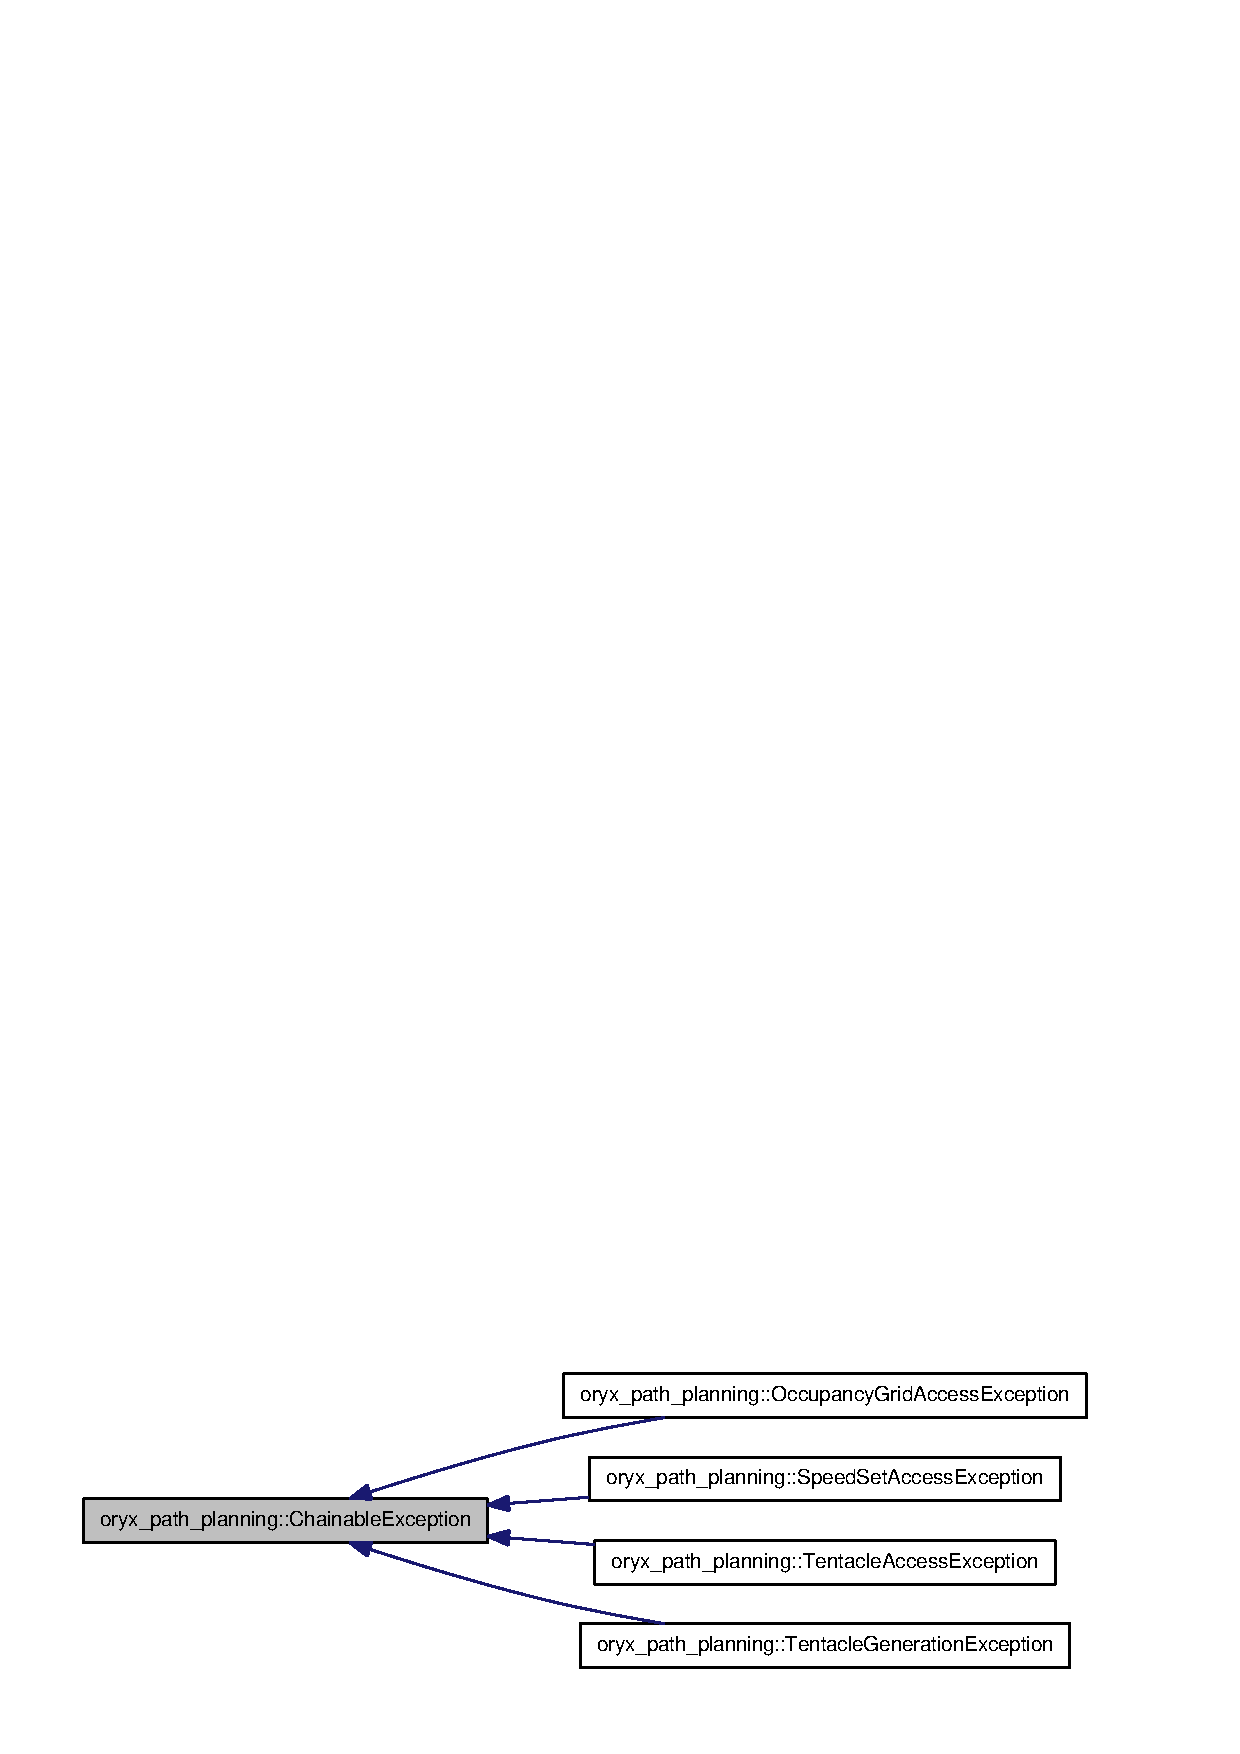
\includegraphics[width=350pt]{classoryx__path__planning_1_1ChainableException__inherit__graph}
\end{center}
\end{figure}
\subsection*{\-Public \-Member \-Functions}
\begin{DoxyCompactItemize}
\item 
{\bf \-Chainable\-Exception} ()
\item 
{\bf \-Chainable\-Exception} ({\bf oryx\-\_\-path\-\_\-planning\-::\-Chainable\-Exception} \&exception)
\item 
{\bf \-Chainable\-Exception} (std\-::string \&message)
\item 
{\bf \-Chainable\-Exception} (std\-::string \&message, std\-::exception \&cause)
\item 
std\-::exception \& {\bf get\-Cause} ()
\item 
{\bf $\sim$\-Chainable\-Exception} ()  throw ()
\end{DoxyCompactItemize}
\subsection*{\-Protected \-Member \-Functions}
\begin{DoxyCompactItemize}
\item 
std\-::string \& {\bf gen\-Message} (std\-::string \&message, std\-::exception \&cause)
\begin{DoxyCompactList}\small\item\em \-The exception which caused this \-Chainged\-Exception. \end{DoxyCompactList}\end{DoxyCompactItemize}
\subsection*{\-Protected \-Attributes}
\begin{DoxyCompactItemize}
\item 
std\-::exception {\bf cause\-\_\-}
\end{DoxyCompactItemize}


\subsection{\-Detailed \-Description}
basic chainable exception class 

\begin{DoxyAuthor}{\-Author}
\-Adam \-Panzics \-Provides an implementation of std\-::exception which allows for chaining of exceptions. \-Returns the chained error message in the form of\-:
\end{DoxyAuthor}
\char`\"{}this\-\_\-message $\backslash$n Caused By-\/$>$ that\-\_\-message\char`\"{} 

\-Definition at line 100 of file \-Oryx\-Path\-Planning\-Utilities.\-h.



\subsection{\-Constructor \& \-Destructor \-Documentation}
\index{oryx\-\_\-path\-\_\-planning\-::\-Chainable\-Exception@{oryx\-\_\-path\-\_\-planning\-::\-Chainable\-Exception}!\-Chainable\-Exception@{\-Chainable\-Exception}}
\index{\-Chainable\-Exception@{\-Chainable\-Exception}!oryx_path_planning::ChainableException@{oryx\-\_\-path\-\_\-planning\-::\-Chainable\-Exception}}
\subsubsection[{\-Chainable\-Exception}]{\setlength{\rightskip}{0pt plus 5cm}{\bf oryx\-\_\-path\-\_\-planning\-::\-Chainable\-Exception\-::\-Chainable\-Exception} (
\begin{DoxyParamCaption}
{}
\end{DoxyParamCaption}
)\hspace{0.3cm}{\ttfamily  [inline]}}\label{classoryx__path__planning_1_1ChainableException_ab20ed6e91591011c1182758900f146f7}
\-Default empty constructor 

\-Definition at line 106 of file \-Oryx\-Path\-Planning\-Utilities.\-h.

\index{oryx\-\_\-path\-\_\-planning\-::\-Chainable\-Exception@{oryx\-\_\-path\-\_\-planning\-::\-Chainable\-Exception}!\-Chainable\-Exception@{\-Chainable\-Exception}}
\index{\-Chainable\-Exception@{\-Chainable\-Exception}!oryx_path_planning::ChainableException@{oryx\-\_\-path\-\_\-planning\-::\-Chainable\-Exception}}
\subsubsection[{\-Chainable\-Exception}]{\setlength{\rightskip}{0pt plus 5cm}{\bf oryx\-\_\-path\-\_\-planning\-::\-Chainable\-Exception\-::\-Chainable\-Exception} (
\begin{DoxyParamCaption}
\item[{{\bf oryx\-\_\-path\-\_\-planning\-::\-Chainable\-Exception} \&}]{exception}
\end{DoxyParamCaption}
)\hspace{0.3cm}{\ttfamily  [inline]}}\label{classoryx__path__planning_1_1ChainableException_a53967498ff29a4debdfb2066db245ef7}
\-Standard \-Copy constructor 
\begin{DoxyParams}{\-Parameters}
{\em exception} & \-The exception to initialize this exception's fields to \\
\hline
\end{DoxyParams}


\-Definition at line 115 of file \-Oryx\-Path\-Planning\-Utilities.\-h.

\index{oryx\-\_\-path\-\_\-planning\-::\-Chainable\-Exception@{oryx\-\_\-path\-\_\-planning\-::\-Chainable\-Exception}!\-Chainable\-Exception@{\-Chainable\-Exception}}
\index{\-Chainable\-Exception@{\-Chainable\-Exception}!oryx_path_planning::ChainableException@{oryx\-\_\-path\-\_\-planning\-::\-Chainable\-Exception}}
\subsubsection[{\-Chainable\-Exception}]{\setlength{\rightskip}{0pt plus 5cm}{\bf oryx\-\_\-path\-\_\-planning\-::\-Chainable\-Exception\-::\-Chainable\-Exception} (
\begin{DoxyParamCaption}
\item[{std\-::string \&}]{message}
\end{DoxyParamCaption}
)\hspace{0.3cm}{\ttfamily  [inline]}}\label{classoryx__path__planning_1_1ChainableException_ac16ccc14c8e8d3b9bcb05d2597155ecb}
\-Constructor for creating a new exception without a cause 
\begin{DoxyParams}{\-Parameters}
{\em message} & \-The error message for this exception \\
\hline
\end{DoxyParams}


\-Definition at line 125 of file \-Oryx\-Path\-Planning\-Utilities.\-h.

\index{oryx\-\_\-path\-\_\-planning\-::\-Chainable\-Exception@{oryx\-\_\-path\-\_\-planning\-::\-Chainable\-Exception}!\-Chainable\-Exception@{\-Chainable\-Exception}}
\index{\-Chainable\-Exception@{\-Chainable\-Exception}!oryx_path_planning::ChainableException@{oryx\-\_\-path\-\_\-planning\-::\-Chainable\-Exception}}
\subsubsection[{\-Chainable\-Exception}]{\setlength{\rightskip}{0pt plus 5cm}{\bf oryx\-\_\-path\-\_\-planning\-::\-Chainable\-Exception\-::\-Chainable\-Exception} (
\begin{DoxyParamCaption}
\item[{std\-::string \&}]{message, }
\item[{std\-::exception \&}]{cause}
\end{DoxyParamCaption}
)\hspace{0.3cm}{\ttfamily  [inline]}}\label{classoryx__path__planning_1_1ChainableException_af4166889087f2f0c2ba7ea9d808b603d}
\-Constructor for creating a new exception with a cause 
\begin{DoxyParams}{\-Parameters}
{\em message} & \-The error message for the exception \\
\hline
{\em cause} & \-The exception which caused this exception \\
\hline
\end{DoxyParams}


\-Definition at line 135 of file \-Oryx\-Path\-Planning\-Utilities.\-h.

\index{oryx\-\_\-path\-\_\-planning\-::\-Chainable\-Exception@{oryx\-\_\-path\-\_\-planning\-::\-Chainable\-Exception}!$\sim$\-Chainable\-Exception@{$\sim$\-Chainable\-Exception}}
\index{$\sim$\-Chainable\-Exception@{$\sim$\-Chainable\-Exception}!oryx_path_planning::ChainableException@{oryx\-\_\-path\-\_\-planning\-::\-Chainable\-Exception}}
\subsubsection[{$\sim$\-Chainable\-Exception}]{\setlength{\rightskip}{0pt plus 5cm}{\bf oryx\-\_\-path\-\_\-planning\-::\-Chainable\-Exception\-::$\sim$\-Chainable\-Exception} (
\begin{DoxyParamCaption}
{}
\end{DoxyParamCaption}
)  throw ()\hspace{0.3cm}{\ttfamily  [inline]}}\label{classoryx__path__planning_1_1ChainableException_a8c231302f56749ee456bdea4b10ced95}


\-Definition at line 141 of file \-Oryx\-Path\-Planning\-Utilities.\-h.



\subsection{\-Member \-Function \-Documentation}
\index{oryx\-\_\-path\-\_\-planning\-::\-Chainable\-Exception@{oryx\-\_\-path\-\_\-planning\-::\-Chainable\-Exception}!gen\-Message@{gen\-Message}}
\index{gen\-Message@{gen\-Message}!oryx_path_planning::ChainableException@{oryx\-\_\-path\-\_\-planning\-::\-Chainable\-Exception}}
\subsubsection[{gen\-Message}]{\setlength{\rightskip}{0pt plus 5cm}std\-::string\& {\bf oryx\-\_\-path\-\_\-planning\-::\-Chainable\-Exception\-::gen\-Message} (
\begin{DoxyParamCaption}
\item[{std\-::string \&}]{message, }
\item[{std\-::exception \&}]{cause}
\end{DoxyParamCaption}
)\hspace{0.3cm}{\ttfamily  [inline, protected]}}\label{classoryx__path__planning_1_1ChainableException_a0633345de372b9a6b09eea3a3db4bd37}


\-The exception which caused this \-Chainged\-Exception. 



\-Definition at line 153 of file \-Oryx\-Path\-Planning\-Utilities.\-h.

\index{oryx\-\_\-path\-\_\-planning\-::\-Chainable\-Exception@{oryx\-\_\-path\-\_\-planning\-::\-Chainable\-Exception}!get\-Cause@{get\-Cause}}
\index{get\-Cause@{get\-Cause}!oryx_path_planning::ChainableException@{oryx\-\_\-path\-\_\-planning\-::\-Chainable\-Exception}}
\subsubsection[{get\-Cause}]{\setlength{\rightskip}{0pt plus 5cm}std\-::exception\& {\bf oryx\-\_\-path\-\_\-planning\-::\-Chainable\-Exception\-::get\-Cause} (
\begin{DoxyParamCaption}
{}
\end{DoxyParamCaption}
)\hspace{0.3cm}{\ttfamily  [inline]}}\label{classoryx__path__planning_1_1ChainableException_a5d5f968075a47a9dd4c477c5a788f5a7}
\-Gets the raw exception that caused this exception \begin{DoxyReturn}{\-Returns}
\-A std\-::exception which caused this exception 
\end{DoxyReturn}


\-Definition at line 147 of file \-Oryx\-Path\-Planning\-Utilities.\-h.



\subsection{\-Member \-Data \-Documentation}
\index{oryx\-\_\-path\-\_\-planning\-::\-Chainable\-Exception@{oryx\-\_\-path\-\_\-planning\-::\-Chainable\-Exception}!cause\-\_\-@{cause\-\_\-}}
\index{cause\-\_\-@{cause\-\_\-}!oryx_path_planning::ChainableException@{oryx\-\_\-path\-\_\-planning\-::\-Chainable\-Exception}}
\subsubsection[{cause\-\_\-}]{\setlength{\rightskip}{0pt plus 5cm}std\-::exception {\bf oryx\-\_\-path\-\_\-planning\-::\-Chainable\-Exception\-::cause\-\_\-}\hspace{0.3cm}{\ttfamily  [protected]}}\label{classoryx__path__planning_1_1ChainableException_a5c1bd8bc4bd38a5bc66b2c29fd48fda9}


\-Definition at line 151 of file \-Oryx\-Path\-Planning\-Utilities.\-h.



\-The documentation for this class was generated from the following file\-:\begin{DoxyCompactItemize}
\item 
{\bf \-Oryx\-Path\-Planning\-Utilities.\-h}\end{DoxyCompactItemize}

\section{\-Command\-Engine \-Class \-Reference}
\label{classCommandEngine}\index{\-Command\-Engine@{\-Command\-Engine}}


\-Command processing engine for the global planner.  


\subsection*{\-Public \-Member \-Functions}
\begin{DoxyCompactItemize}
\item 
{\bf \-Command\-Engine} ()
\begin{DoxyCompactList}\small\item\em \-Typedef for a map of command functions to their command keyword. \end{DoxyCompactList}\item 
{\bf \-Command\-Engine} (ros\-::\-Node\-Handle \&nh)
\item 
virtual {\bf $\sim$\-Command\-Engine} ()
\end{DoxyCompactItemize}
\subsection*{\-Private \-Types}
\begin{DoxyCompactItemize}
\item 
typedef enum \*
{\bf \-Command\-Engine\-::command\-\_\-criticality\-\_\-} {\bf command\-\_\-criticality}
\item 
enum {\bf command\-\_\-criticality\-\_\-} \{ {\bf \-F\-A\-T\-A\-L}, 
{\bf \-C\-R\-I\-T\-I\-C\-A\-L}, 
{\bf \-W\-A\-R\-N\-I\-N\-G}
 \}
\item 
typedef boost\-::function$<$ bool(std\-::string \*
\&data, \*
oryxsrr\-\_\-msgs\-::\-Command\-::\-Response \*
\&response)$>$ {\bf command\-\_\-func}
\item 
typedef boost\-::unordered\-\_\-map\*
$<$ std\-::string, std\-::pair\*
$<$ {\bf command\-\_\-func}, \*
{\bf command\-\_\-criticality} $>$ $>$ {\bf command\-\_\-map}
\begin{DoxyCompactList}\small\item\em \-Typedef for the signature of command functions. \end{DoxyCompactList}\end{DoxyCompactItemize}
\subsection*{\-Private \-Member \-Functions}
\begin{DoxyCompactItemize}
\item 
bool {\bf auto\-C\-B} (std\-::string \&data, oryxsrr\-\_\-msgs\-::\-Command\-::\-Response \&response)
\item 
void {\bf bind\-Commands} ()
\item 
bool {\bf command\-C\-B} (oryxsrr\-\_\-msgs\-::\-Command\-::\-Request \&request, oryxsrr\-\_\-msgs\-::\-Command\-::\-Response \&response)
\item 
void {\bf init} ()
\item 
bool {\bf man\-C\-B} (std\-::string \&data, oryxsrr\-\_\-msgs\-::\-Command\-::\-Response \&response)
\item 
bool {\bf start\-C\-B} (std\-::string \&data, oryxsrr\-\_\-msgs\-::\-Command\-::\-Response \&response)
\item 
bool {\bf stop\-C\-B} (std\-::string \&data, oryxsrr\-\_\-msgs\-::\-Command\-::\-Response \&response)
\end{DoxyCompactItemize}
\subsection*{\-Private \-Attributes}
\begin{DoxyCompactItemize}
\item 
{\bf command\-\_\-map} {\bf com\-\_\-map\-\_\-}
\begin{DoxyCompactList}\small\item\em \-Service \-Server for processing \-Command services. \end{DoxyCompactList}\item 
ros\-::\-Service\-Server {\bf comm\-\_\-srv\-\_\-}
\begin{DoxyCompactList}\small\item\em \-Node handle for communicating with \-R\-O\-S system. \end{DoxyCompactList}\item 
ros\-::\-Node\-Handle {\bf nh\-\_\-}
\end{DoxyCompactItemize}


\subsection{\-Detailed \-Description}
\-Command processing engine for the global planner. 

\begin{DoxyAuthor}{\-Author}
\-Adam \-Panzica
\end{DoxyAuthor}
\-A class defining a series of commands, and their respective callbacks, that allows the the global planner to communicate with a client node. \-Its intention is to allow for the control of the global planner via remote connection during runtime, for debugging and safety reasons. 

\-Definition at line 28 of file oryx\-\_\-global\-\_\-planner.\-cpp.



\subsection{\-Member \-Typedef \-Documentation}
\index{\-Command\-Engine@{\-Command\-Engine}!command\-\_\-criticality@{command\-\_\-criticality}}
\index{command\-\_\-criticality@{command\-\_\-criticality}!CommandEngine@{\-Command\-Engine}}
\subsubsection[{command\-\_\-criticality}]{\setlength{\rightskip}{0pt plus 5cm}typedef enum {\bf \-Command\-Engine\-::command\-\_\-criticality\-\_\-}  {\bf \-Command\-Engine\-::command\-\_\-criticality}\hspace{0.3cm}{\ttfamily  [private]}}\label{classCommandEngine_aa7b7491a106ead128f57e82cf15f114d}
\-Enum defining the levels of criticality for command functions \index{\-Command\-Engine@{\-Command\-Engine}!command\-\_\-func@{command\-\_\-func}}
\index{command\-\_\-func@{command\-\_\-func}!CommandEngine@{\-Command\-Engine}}
\subsubsection[{command\-\_\-func}]{\setlength{\rightskip}{0pt plus 5cm}typedef boost\-::function$<$bool (std\-::string\& data, oryxsrr\-\_\-msgs\-::\-Command\-::\-Response\& response)$>$ {\bf \-Command\-Engine\-::command\-\_\-func}\hspace{0.3cm}{\ttfamily  [private]}}\label{classCommandEngine_a9b4477e847b3fcf29b2417536a89f9e3}


\-Definition at line 41 of file oryx\-\_\-global\-\_\-planner.\-cpp.

\index{\-Command\-Engine@{\-Command\-Engine}!command\-\_\-map@{command\-\_\-map}}
\index{command\-\_\-map@{command\-\_\-map}!CommandEngine@{\-Command\-Engine}}
\subsubsection[{command\-\_\-map}]{\setlength{\rightskip}{0pt plus 5cm}typedef boost\-::unordered\-\_\-map$<$std\-::string, std\-::pair$<${\bf command\-\_\-func}, {\bf command\-\_\-criticality}$>$ $>$ {\bf \-Command\-Engine\-::command\-\_\-map}\hspace{0.3cm}{\ttfamily  [private]}}\label{classCommandEngine_a7cf96b4908314b5d7e2f0f5c01469466}


\-Typedef for the signature of command functions. 



\-Definition at line 42 of file oryx\-\_\-global\-\_\-planner.\-cpp.



\subsection{\-Member \-Enumeration \-Documentation}
\index{\-Command\-Engine@{\-Command\-Engine}!command\-\_\-criticality\-\_\-@{command\-\_\-criticality\-\_\-}}
\index{command\-\_\-criticality\-\_\-@{command\-\_\-criticality\-\_\-}!CommandEngine@{\-Command\-Engine}}
\subsubsection[{command\-\_\-criticality\-\_\-}]{\setlength{\rightskip}{0pt plus 5cm}enum {\bf \-Command\-Engine\-::command\-\_\-criticality\-\_\-}\hspace{0.3cm}{\ttfamily  [private]}}\label{classCommandEngine_a239753fb905a092ffb4225c9484840b6}
\-Enum defining the levels of criticality for command functions \begin{Desc}
\item[\-Enumerator\-: ]\par
\begin{description}
\index{\-F\-A\-T\-A\-L@{\-F\-A\-T\-A\-L}!\-Command\-Engine@{\-Command\-Engine}}\index{\-Command\-Engine@{\-Command\-Engine}!\-F\-A\-T\-A\-L@{\-F\-A\-T\-A\-L}}\item[{\em 
\-F\-A\-T\-A\-L\label{classCommandEngine_a239753fb905a092ffb4225c9484840b6afd3d386213dfbf368e96020f54aa1d5a}
}]\-F\-A\-T\-A\-L \-Failure to process the command is a fatal error. \index{\-C\-R\-I\-T\-I\-C\-A\-L@{\-C\-R\-I\-T\-I\-C\-A\-L}!\-Command\-Engine@{\-Command\-Engine}}\index{\-Command\-Engine@{\-Command\-Engine}!\-C\-R\-I\-T\-I\-C\-A\-L@{\-C\-R\-I\-T\-I\-C\-A\-L}}\item[{\em 
\-C\-R\-I\-T\-I\-C\-A\-L\label{classCommandEngine_a239753fb905a092ffb4225c9484840b6a8fd1df97b99b4b8f3ce6369248651a28}
}]\-C\-R\-I\-T\-I\-C\-A\-L \-Failure to process the command is a critical error. \index{\-W\-A\-R\-N\-I\-N\-G@{\-W\-A\-R\-N\-I\-N\-G}!\-Command\-Engine@{\-Command\-Engine}}\index{\-Command\-Engine@{\-Command\-Engine}!\-W\-A\-R\-N\-I\-N\-G@{\-W\-A\-R\-N\-I\-N\-G}}\item[{\em 
\-W\-A\-R\-N\-I\-N\-G\label{classCommandEngine_a239753fb905a092ffb4225c9484840b6ae8273610bb844c439ae477ce5d7ba626}
}]\-W\-A\-R\-N\-I\-N\-G \-Failure to process the command is only a warning. \end{description}
\end{Desc}



\-Definition at line 34 of file oryx\-\_\-global\-\_\-planner.\-cpp.



\subsection{\-Constructor \& \-Destructor \-Documentation}
\index{\-Command\-Engine@{\-Command\-Engine}!\-Command\-Engine@{\-Command\-Engine}}
\index{\-Command\-Engine@{\-Command\-Engine}!CommandEngine@{\-Command\-Engine}}
\subsubsection[{\-Command\-Engine}]{\setlength{\rightskip}{0pt plus 5cm}{\bf \-Command\-Engine\-::\-Command\-Engine} (
\begin{DoxyParamCaption}
{}
\end{DoxyParamCaption}
)\hspace{0.3cm}{\ttfamily  [inline]}}\label{classCommandEngine_a57c2ecba8bfc073b7bb72788a6ab653a}


\-Typedef for a map of command functions to their command keyword. 



\-Definition at line 44 of file oryx\-\_\-global\-\_\-planner.\-cpp.

\index{\-Command\-Engine@{\-Command\-Engine}!\-Command\-Engine@{\-Command\-Engine}}
\index{\-Command\-Engine@{\-Command\-Engine}!CommandEngine@{\-Command\-Engine}}
\subsubsection[{\-Command\-Engine}]{\setlength{\rightskip}{0pt plus 5cm}{\bf \-Command\-Engine\-::\-Command\-Engine} (
\begin{DoxyParamCaption}
\item[{ros\-::\-Node\-Handle \&}]{nh}
\end{DoxyParamCaption}
)\hspace{0.3cm}{\ttfamily  [inline]}}\label{classCommandEngine_a9925f5fa145f51094f5fab3207f95ca0}


\-Definition at line 49 of file oryx\-\_\-global\-\_\-planner.\-cpp.

\index{\-Command\-Engine@{\-Command\-Engine}!$\sim$\-Command\-Engine@{$\sim$\-Command\-Engine}}
\index{$\sim$\-Command\-Engine@{$\sim$\-Command\-Engine}!CommandEngine@{\-Command\-Engine}}
\subsubsection[{$\sim$\-Command\-Engine}]{\setlength{\rightskip}{0pt plus 5cm}virtual {\bf \-Command\-Engine\-::$\sim$\-Command\-Engine} (
\begin{DoxyParamCaption}
{}
\end{DoxyParamCaption}
)\hspace{0.3cm}{\ttfamily  [inline, virtual]}}\label{classCommandEngine_aa4ef8440059fe2ae268f151c2229e733}


\-Definition at line 55 of file oryx\-\_\-global\-\_\-planner.\-cpp.



\subsection{\-Member \-Function \-Documentation}
\index{\-Command\-Engine@{\-Command\-Engine}!auto\-C\-B@{auto\-C\-B}}
\index{auto\-C\-B@{auto\-C\-B}!CommandEngine@{\-Command\-Engine}}
\subsubsection[{auto\-C\-B}]{\setlength{\rightskip}{0pt plus 5cm}bool {\bf \-Command\-Engine\-::auto\-C\-B} (
\begin{DoxyParamCaption}
\item[{std\-::string \&}]{data, }
\item[{oryxsrr\-\_\-msgs\-::\-Command\-::\-Response \&}]{response}
\end{DoxyParamCaption}
)\hspace{0.3cm}{\ttfamily  [inline, private]}}\label{classCommandEngine_aca9663d2ab6fe972b7442a6258b513a1}
\-Callback for processing the \char`\"{}autonomous\char`\"{} command \begin{DoxyAuthor}{\-Author}
\-Adam \-Panzica 
\end{DoxyAuthor}

\begin{DoxyParams}{\-Parameters}
{\em data} & \-Command data to be parsed \\
\hline
\end{DoxyParams}
\begin{DoxyReturn}{\-Returns}
\-T\-R\-U\-E if the command successfully processed, else \-F\-A\-L\-S\-E
\end{DoxyReturn}
\-This command puts the global planner into \-Autonomous \-Control mode. 

\-Definition at line 191 of file oryx\-\_\-global\-\_\-planner.\-cpp.

\index{\-Command\-Engine@{\-Command\-Engine}!bind\-Commands@{bind\-Commands}}
\index{bind\-Commands@{bind\-Commands}!CommandEngine@{\-Command\-Engine}}
\subsubsection[{bind\-Commands}]{\setlength{\rightskip}{0pt plus 5cm}void {\bf \-Command\-Engine\-::bind\-Commands} (
\begin{DoxyParamCaption}
{}
\end{DoxyParamCaption}
)\hspace{0.3cm}{\ttfamily  [inline, private]}}\label{classCommandEngine_a40e7e3bd5795559eecf6782a8f75b7a9}
\-Registers all of the commands with their processing callback 

\-Definition at line 76 of file oryx\-\_\-global\-\_\-planner.\-cpp.

\index{\-Command\-Engine@{\-Command\-Engine}!command\-C\-B@{command\-C\-B}}
\index{command\-C\-B@{command\-C\-B}!CommandEngine@{\-Command\-Engine}}
\subsubsection[{command\-C\-B}]{\setlength{\rightskip}{0pt plus 5cm}bool {\bf \-Command\-Engine\-::command\-C\-B} (
\begin{DoxyParamCaption}
\item[{oryxsrr\-\_\-msgs\-::\-Command\-::\-Request \&}]{request, }
\item[{oryxsrr\-\_\-msgs\-::\-Command\-::\-Response \&}]{response}
\end{DoxyParamCaption}
)\hspace{0.3cm}{\ttfamily  [inline, private]}}\label{classCommandEngine_a86930ff926dfdb4c03a4671f498be709}
\-Callback for processing received commands \begin{DoxyAuthor}{\-Author}
\-Adam \-Panzica 
\end{DoxyAuthor}

\begin{DoxyParams}{\-Parameters}
{\em request} & \-The service request \\
\hline
{\em response} & \-The service response \\
\hline
\end{DoxyParams}


\-Definition at line 103 of file oryx\-\_\-global\-\_\-planner.\-cpp.

\index{\-Command\-Engine@{\-Command\-Engine}!init@{init}}
\index{init@{init}!CommandEngine@{\-Command\-Engine}}
\subsubsection[{init}]{\setlength{\rightskip}{0pt plus 5cm}void {\bf \-Command\-Engine\-::init} (
\begin{DoxyParamCaption}
{}
\end{DoxyParamCaption}
)\hspace{0.3cm}{\ttfamily  [inline, private]}}\label{classCommandEngine_a7a4b467ac31cbfa470ca5e19e7cef0e5}
\-Perform common initialization 

\-Definition at line 69 of file oryx\-\_\-global\-\_\-planner.\-cpp.

\index{\-Command\-Engine@{\-Command\-Engine}!man\-C\-B@{man\-C\-B}}
\index{man\-C\-B@{man\-C\-B}!CommandEngine@{\-Command\-Engine}}
\subsubsection[{man\-C\-B}]{\setlength{\rightskip}{0pt plus 5cm}bool {\bf \-Command\-Engine\-::man\-C\-B} (
\begin{DoxyParamCaption}
\item[{std\-::string \&}]{data, }
\item[{oryxsrr\-\_\-msgs\-::\-Command\-::\-Response \&}]{response}
\end{DoxyParamCaption}
)\hspace{0.3cm}{\ttfamily  [inline, private]}}\label{classCommandEngine_a234ae5fd6dbd512b7e730f0c46f9046b}
\-Callback for processing the \char`\"{}manual\char`\"{} command \begin{DoxyAuthor}{\-Author}
\-Adam \-Panzica 
\end{DoxyAuthor}

\begin{DoxyParams}{\-Parameters}
{\em data} & \-Command data to be parsed \\
\hline
\end{DoxyParams}
\begin{DoxyReturn}{\-Returns}
\-T\-R\-U\-E if the command successfully processed, else \-F\-A\-L\-S\-E
\end{DoxyReturn}
\-This command puts the global planner into \-Manual \-Control mode. \-It lets it know to expect \-Joy \-Messages to control it 

\-Definition at line 178 of file oryx\-\_\-global\-\_\-planner.\-cpp.

\index{\-Command\-Engine@{\-Command\-Engine}!start\-C\-B@{start\-C\-B}}
\index{start\-C\-B@{start\-C\-B}!CommandEngine@{\-Command\-Engine}}
\subsubsection[{start\-C\-B}]{\setlength{\rightskip}{0pt plus 5cm}bool {\bf \-Command\-Engine\-::start\-C\-B} (
\begin{DoxyParamCaption}
\item[{std\-::string \&}]{data, }
\item[{oryxsrr\-\_\-msgs\-::\-Command\-::\-Response \&}]{response}
\end{DoxyParamCaption}
)\hspace{0.3cm}{\ttfamily  [inline, private]}}\label{classCommandEngine_a60ffb4e1bf17dc41f8ca3840ecca9ecb}
\-Callback for processing the \char`\"{}start\char`\"{} command \begin{DoxyAuthor}{\-Author}
\-Adam \-Panzica 
\end{DoxyAuthor}

\begin{DoxyParams}{\-Parameters}
{\em data} & \-Command data to be parsed \\
\hline
\end{DoxyParams}
\begin{DoxyReturn}{\-Returns}
\-T\-R\-U\-E if the command successfully processed, else \-F\-A\-L\-S\-E
\end{DoxyReturn}
\-This command starts the global planner into whatever mode it was in last (or default if there was no mode specified) 

\-Definition at line 151 of file oryx\-\_\-global\-\_\-planner.\-cpp.

\index{\-Command\-Engine@{\-Command\-Engine}!stop\-C\-B@{stop\-C\-B}}
\index{stop\-C\-B@{stop\-C\-B}!CommandEngine@{\-Command\-Engine}}
\subsubsection[{stop\-C\-B}]{\setlength{\rightskip}{0pt plus 5cm}bool {\bf \-Command\-Engine\-::stop\-C\-B} (
\begin{DoxyParamCaption}
\item[{std\-::string \&}]{data, }
\item[{oryxsrr\-\_\-msgs\-::\-Command\-::\-Response \&}]{response}
\end{DoxyParamCaption}
)\hspace{0.3cm}{\ttfamily  [inline, private]}}\label{classCommandEngine_aa0cddceda1c3fa208fdfa657a7cf27f9}
\-Callback for processing the \char`\"{}start\char`\"{} command \begin{DoxyAuthor}{\-Author}
\-Adam \-Panzica 
\end{DoxyAuthor}

\begin{DoxyParams}{\-Parameters}
{\em data} & \-Command data to be parsed \\
\hline
\end{DoxyParams}
\begin{DoxyReturn}{\-Returns}
\-T\-R\-U\-E if the command successfully processed, else \-F\-A\-L\-S\-E
\end{DoxyReturn}
\-This command stops the global planner from running, except to process new commands from the \doxyref{\-Command\-Engine}{p.}{classCommandEngine} 

\-Definition at line 164 of file oryx\-\_\-global\-\_\-planner.\-cpp.



\subsection{\-Member \-Data \-Documentation}
\index{\-Command\-Engine@{\-Command\-Engine}!com\-\_\-map\-\_\-@{com\-\_\-map\-\_\-}}
\index{com\-\_\-map\-\_\-@{com\-\_\-map\-\_\-}!CommandEngine@{\-Command\-Engine}}
\subsubsection[{com\-\_\-map\-\_\-}]{\setlength{\rightskip}{0pt plus 5cm}{\bf command\-\_\-map} {\bf \-Command\-Engine\-::com\-\_\-map\-\_\-}\hspace{0.3cm}{\ttfamily  [private]}}\label{classCommandEngine_a6aaa5a8dac874a4179e4d4cd34dd3f0d}


\-Service \-Server for processing \-Command services. 

\-Mapping of command functions to their string keyword. \-Each command has a integer criticality associated with it, which can be used to judge the consequences of commands failing 

\-Definition at line 64 of file oryx\-\_\-global\-\_\-planner.\-cpp.

\index{\-Command\-Engine@{\-Command\-Engine}!comm\-\_\-srv\-\_\-@{comm\-\_\-srv\-\_\-}}
\index{comm\-\_\-srv\-\_\-@{comm\-\_\-srv\-\_\-}!CommandEngine@{\-Command\-Engine}}
\subsubsection[{comm\-\_\-srv\-\_\-}]{\setlength{\rightskip}{0pt plus 5cm}ros\-::\-Service\-Server {\bf \-Command\-Engine\-::comm\-\_\-srv\-\_\-}\hspace{0.3cm}{\ttfamily  [private]}}\label{classCommandEngine_abf2fbdc657fe71432b3950df90cc2994}


\-Node handle for communicating with \-R\-O\-S system. 



\-Definition at line 58 of file oryx\-\_\-global\-\_\-planner.\-cpp.

\index{\-Command\-Engine@{\-Command\-Engine}!nh\-\_\-@{nh\-\_\-}}
\index{nh\-\_\-@{nh\-\_\-}!CommandEngine@{\-Command\-Engine}}
\subsubsection[{nh\-\_\-}]{\setlength{\rightskip}{0pt plus 5cm}ros\-::\-Node\-Handle {\bf \-Command\-Engine\-::nh\-\_\-}\hspace{0.3cm}{\ttfamily  [private]}}\label{classCommandEngine_aee411227d737967135532d617a0ae4cd}


\-Definition at line 55 of file oryx\-\_\-global\-\_\-planner.\-cpp.



\-The documentation for this class was generated from the following file\-:\begin{DoxyCompactItemize}
\item 
{\bf oryx\-\_\-global\-\_\-planner.\-cpp}\end{DoxyCompactItemize}

\section{oryx\-\_\-path\-\_\-planning\-:\-:constants \-Class \-Reference}
\label{classoryx__path__planning_1_1constants}\index{oryx\-\_\-path\-\_\-planning\-::constants@{oryx\-\_\-path\-\_\-planning\-::constants}}


singleton class which returns dynamically generated constants  




{\ttfamily \#include $<$\-Oryx\-Path\-Planning\-Utilities.\-h$>$}

\subsection*{\-Static \-Public \-Member \-Functions}
\begin{DoxyCompactItemize}
\item 
static double {\bf \-P\-I} ()
\end{DoxyCompactItemize}


\subsection{\-Detailed \-Description}
singleton class which returns dynamically generated constants 

\begin{DoxyAuthor}{\-Author}
\-Adam \-Panzica 
\end{DoxyAuthor}


\-Definition at line 60 of file \-Oryx\-Path\-Planning\-Utilities.\-h.



\subsection{\-Member \-Function \-Documentation}
\index{oryx\-\_\-path\-\_\-planning\-::constants@{oryx\-\_\-path\-\_\-planning\-::constants}!\-P\-I@{\-P\-I}}
\index{\-P\-I@{\-P\-I}!oryx_path_planning::constants@{oryx\-\_\-path\-\_\-planning\-::constants}}
\subsubsection[{\-P\-I}]{\setlength{\rightskip}{0pt plus 5cm}static double {\bf oryx\-\_\-path\-\_\-planning\-::constants\-::\-P\-I} (
\begin{DoxyParamCaption}
{}
\end{DoxyParamCaption}
)\hspace{0.3cm}{\ttfamily  [inline, static]}}\label{classoryx__path__planning_1_1constants_a4543e76cf5aaf0899fd0a6536f26e828}
\-Since \-C++ lacks a predefined \-P\-I constant, define it here 

\-Definition at line 63 of file \-Oryx\-Path\-Planning\-Utilities.\-h.



\-The documentation for this class was generated from the following file\-:\begin{DoxyCompactItemize}
\item 
{\bf \-Oryx\-Path\-Planning\-Utilities.\-h}\end{DoxyCompactItemize}

\section{ros\-:\-:message\-\_\-traits\-:\-:\-Data\-Type$<$ \-:\-:oryx\-\_\-path\-\_\-planning\-:\-:\-Occupancy\-Grid\-\_\-$<$ \-Container\-Allocator $>$ $>$ \-Struct \-Template \-Reference}
\label{structros_1_1message__traits_1_1DataType_3_01_1_1oryx__path__planning_1_1OccupancyGrid___3_01ContainerAllocator_01_4_01_4}\index{ros\-::message\-\_\-traits\-::\-Data\-Type$<$ \-::oryx\-\_\-path\-\_\-planning\-::\-Occupancy\-Grid\-\_\-$<$ Container\-Allocator $>$ $>$@{ros\-::message\-\_\-traits\-::\-Data\-Type$<$ \-::oryx\-\_\-path\-\_\-planning\-::\-Occupancy\-Grid\-\_\-$<$ Container\-Allocator $>$ $>$}}


{\ttfamily \#include $<$\-Occupancy\-Grid.\-h$>$}

\subsection*{\-Static \-Public \-Member \-Functions}
\begin{DoxyCompactItemize}
\item 
static const char $\ast$ {\bf value} ()
\item 
static const char $\ast$ {\bf value} (const \-::{\bf oryx\-\_\-path\-\_\-planning\-::\-Occupancy\-Grid\-\_\-}$<$ \-Container\-Allocator $>$ \&)
\end{DoxyCompactItemize}


\subsection{\-Detailed \-Description}
\subsubsection*{template$<$class Container\-Allocator$>$struct ros\-::message\-\_\-traits\-::\-Data\-Type$<$ \-::oryx\-\_\-path\-\_\-planning\-::\-Occupancy\-Grid\-\_\-$<$ Container\-Allocator $>$ $>$}



\-Definition at line 137 of file msg\-\_\-gen/cpp/include/oryx\-\_\-path\-\_\-planning/\-Occupancy\-Grid.\-h.



\subsection{\-Member \-Function \-Documentation}
\index{ros\-::message\-\_\-traits\-::\-Data\-Type$<$ \-::oryx\-\_\-path\-\_\-planning\-::\-Occupancy\-Grid\-\_\-$<$ Container\-Allocator $>$ $>$@{ros\-::message\-\_\-traits\-::\-Data\-Type$<$ \-::oryx\-\_\-path\-\_\-planning\-::\-Occupancy\-Grid\-\_\-$<$ Container\-Allocator $>$ $>$}!value@{value}}
\index{value@{value}!ros::message_traits::DataType< ::oryx_path_planning::OccupancyGrid_< ContainerAllocator > >@{ros\-::message\-\_\-traits\-::\-Data\-Type$<$ \-::oryx\-\_\-path\-\_\-planning\-::\-Occupancy\-Grid\-\_\-$<$ Container\-Allocator $>$ $>$}}
\subsubsection[{value}]{\setlength{\rightskip}{0pt plus 5cm}template$<$class Container\-Allocator $>$ static const char$\ast$ ros\-::message\-\_\-traits\-::\-Data\-Type$<$ \-::{\bf oryx\-\_\-path\-\_\-planning\-::\-Occupancy\-Grid\-\_\-}$<$ \-Container\-Allocator $>$ $>$\-::{\bf value} (
\begin{DoxyParamCaption}
{}
\end{DoxyParamCaption}
)\hspace{0.3cm}{\ttfamily  [inline, static]}}\label{structros_1_1message__traits_1_1DataType_3_01_1_1oryx__path__planning_1_1OccupancyGrid___3_01ContainerAllocator_01_4_01_4_ae1e4a0b13f2b09a69133502a31e9c2ec}


\-Definition at line 138 of file msg\-\_\-gen/cpp/include/oryx\-\_\-path\-\_\-planning/\-Occupancy\-Grid.\-h.

\index{ros\-::message\-\_\-traits\-::\-Data\-Type$<$ \-::oryx\-\_\-path\-\_\-planning\-::\-Occupancy\-Grid\-\_\-$<$ Container\-Allocator $>$ $>$@{ros\-::message\-\_\-traits\-::\-Data\-Type$<$ \-::oryx\-\_\-path\-\_\-planning\-::\-Occupancy\-Grid\-\_\-$<$ Container\-Allocator $>$ $>$}!value@{value}}
\index{value@{value}!ros::message_traits::DataType< ::oryx_path_planning::OccupancyGrid_< ContainerAllocator > >@{ros\-::message\-\_\-traits\-::\-Data\-Type$<$ \-::oryx\-\_\-path\-\_\-planning\-::\-Occupancy\-Grid\-\_\-$<$ Container\-Allocator $>$ $>$}}
\subsubsection[{value}]{\setlength{\rightskip}{0pt plus 5cm}template$<$class Container\-Allocator $>$ static const char$\ast$ ros\-::message\-\_\-traits\-::\-Data\-Type$<$ \-::{\bf oryx\-\_\-path\-\_\-planning\-::\-Occupancy\-Grid\-\_\-}$<$ \-Container\-Allocator $>$ $>$\-::{\bf value} (
\begin{DoxyParamCaption}
\item[{const \-::{\bf oryx\-\_\-path\-\_\-planning\-::\-Occupancy\-Grid\-\_\-}$<$ \-Container\-Allocator $>$ \&}]{}
\end{DoxyParamCaption}
)\hspace{0.3cm}{\ttfamily  [inline, static]}}\label{structros_1_1message__traits_1_1DataType_3_01_1_1oryx__path__planning_1_1OccupancyGrid___3_01ContainerAllocator_01_4_01_4_a892e53155911a6a658a8596f53f67ebd}


\-Definition at line 143 of file msg\-\_\-gen/cpp/include/oryx\-\_\-path\-\_\-planning/\-Occupancy\-Grid.\-h.



\-The documentation for this struct was generated from the following file\-:\begin{DoxyCompactItemize}
\item 
{\bf msg\-\_\-gen/cpp/include/oryx\-\_\-path\-\_\-planning/\-Occupancy\-Grid.\-h}\end{DoxyCompactItemize}

\section{ros\-:\-:message\-\_\-traits\-:\-:\-Data\-Type$<$ \-:\-:oryx\-\_\-path\-\_\-planning\-:\-:\-Occupancy\-Grid\-Msg\-\_\-$<$ \-Container\-Allocator $>$ $>$ \-Struct \-Template \-Reference}
\label{structros_1_1message__traits_1_1DataType_3_01_1_1oryx__path__planning_1_1OccupancyGridMsg___3_01ContainerAllocator_01_4_01_4}\index{ros\-::message\-\_\-traits\-::\-Data\-Type$<$ \-::oryx\-\_\-path\-\_\-planning\-::\-Occupancy\-Grid\-Msg\-\_\-$<$ Container\-Allocator $>$ $>$@{ros\-::message\-\_\-traits\-::\-Data\-Type$<$ \-::oryx\-\_\-path\-\_\-planning\-::\-Occupancy\-Grid\-Msg\-\_\-$<$ Container\-Allocator $>$ $>$}}


{\ttfamily \#include $<$\-Occupancy\-Grid\-Msg.\-h$>$}

\subsection*{\-Static \-Public \-Member \-Functions}
\begin{DoxyCompactItemize}
\item 
static const char $\ast$ {\bf value} ()
\item 
static const char $\ast$ {\bf value} (const \-::{\bf oryx\-\_\-path\-\_\-planning\-::\-Occupancy\-Grid\-Msg\-\_\-}$<$ \-Container\-Allocator $>$ \&)
\end{DoxyCompactItemize}


\subsection{\-Detailed \-Description}
\subsubsection*{template$<$class Container\-Allocator$>$struct ros\-::message\-\_\-traits\-::\-Data\-Type$<$ \-::oryx\-\_\-path\-\_\-planning\-::\-Occupancy\-Grid\-Msg\-\_\-$<$ Container\-Allocator $>$ $>$}



\-Definition at line 137 of file \-Occupancy\-Grid\-Msg.\-h.



\subsection{\-Member \-Function \-Documentation}
\index{ros\-::message\-\_\-traits\-::\-Data\-Type$<$ \-::oryx\-\_\-path\-\_\-planning\-::\-Occupancy\-Grid\-Msg\-\_\-$<$ Container\-Allocator $>$ $>$@{ros\-::message\-\_\-traits\-::\-Data\-Type$<$ \-::oryx\-\_\-path\-\_\-planning\-::\-Occupancy\-Grid\-Msg\-\_\-$<$ Container\-Allocator $>$ $>$}!value@{value}}
\index{value@{value}!ros::message_traits::DataType< ::oryx_path_planning::OccupancyGridMsg_< ContainerAllocator > >@{ros\-::message\-\_\-traits\-::\-Data\-Type$<$ \-::oryx\-\_\-path\-\_\-planning\-::\-Occupancy\-Grid\-Msg\-\_\-$<$ Container\-Allocator $>$ $>$}}
\subsubsection[{value}]{\setlength{\rightskip}{0pt plus 5cm}template$<$class Container\-Allocator $>$ static const char$\ast$ ros\-::message\-\_\-traits\-::\-Data\-Type$<$ \-::{\bf oryx\-\_\-path\-\_\-planning\-::\-Occupancy\-Grid\-Msg\-\_\-}$<$ \-Container\-Allocator $>$ $>$\-::{\bf value} (
\begin{DoxyParamCaption}
{}
\end{DoxyParamCaption}
)\hspace{0.3cm}{\ttfamily  [inline, static]}}\label{structros_1_1message__traits_1_1DataType_3_01_1_1oryx__path__planning_1_1OccupancyGridMsg___3_01ContainerAllocator_01_4_01_4_a40809dc29de95ac4ccd2d75d1f431a28}


\-Definition at line 138 of file \-Occupancy\-Grid\-Msg.\-h.

\index{ros\-::message\-\_\-traits\-::\-Data\-Type$<$ \-::oryx\-\_\-path\-\_\-planning\-::\-Occupancy\-Grid\-Msg\-\_\-$<$ Container\-Allocator $>$ $>$@{ros\-::message\-\_\-traits\-::\-Data\-Type$<$ \-::oryx\-\_\-path\-\_\-planning\-::\-Occupancy\-Grid\-Msg\-\_\-$<$ Container\-Allocator $>$ $>$}!value@{value}}
\index{value@{value}!ros::message_traits::DataType< ::oryx_path_planning::OccupancyGridMsg_< ContainerAllocator > >@{ros\-::message\-\_\-traits\-::\-Data\-Type$<$ \-::oryx\-\_\-path\-\_\-planning\-::\-Occupancy\-Grid\-Msg\-\_\-$<$ Container\-Allocator $>$ $>$}}
\subsubsection[{value}]{\setlength{\rightskip}{0pt plus 5cm}template$<$class Container\-Allocator $>$ static const char$\ast$ ros\-::message\-\_\-traits\-::\-Data\-Type$<$ \-::{\bf oryx\-\_\-path\-\_\-planning\-::\-Occupancy\-Grid\-Msg\-\_\-}$<$ \-Container\-Allocator $>$ $>$\-::{\bf value} (
\begin{DoxyParamCaption}
\item[{const \-::{\bf oryx\-\_\-path\-\_\-planning\-::\-Occupancy\-Grid\-Msg\-\_\-}$<$ \-Container\-Allocator $>$ \&}]{}
\end{DoxyParamCaption}
)\hspace{0.3cm}{\ttfamily  [inline, static]}}\label{structros_1_1message__traits_1_1DataType_3_01_1_1oryx__path__planning_1_1OccupancyGridMsg___3_01ContainerAllocator_01_4_01_4_a448afe35ae3512c3f69ce22b396dec5b}


\-Definition at line 143 of file \-Occupancy\-Grid\-Msg.\-h.



\-The documentation for this struct was generated from the following file\-:\begin{DoxyCompactItemize}
\item 
{\bf \-Occupancy\-Grid\-Msg.\-h}\end{DoxyCompactItemize}

\section{ros\-:\-:message\-\_\-traits\-:\-:\-Definition$<$ \-:\-:oryx\-\_\-path\-\_\-planning\-:\-:\-Occupancy\-Grid\-\_\-$<$ \-Container\-Allocator $>$ $>$ \-Struct \-Template \-Reference}
\label{structros_1_1message__traits_1_1Definition_3_01_1_1oryx__path__planning_1_1OccupancyGrid___3_01ContainerAllocator_01_4_01_4}\index{ros\-::message\-\_\-traits\-::\-Definition$<$ \-::oryx\-\_\-path\-\_\-planning\-::\-Occupancy\-Grid\-\_\-$<$ Container\-Allocator $>$ $>$@{ros\-::message\-\_\-traits\-::\-Definition$<$ \-::oryx\-\_\-path\-\_\-planning\-::\-Occupancy\-Grid\-\_\-$<$ Container\-Allocator $>$ $>$}}


{\ttfamily \#include $<$\-Occupancy\-Grid.\-h$>$}

\subsection*{\-Static \-Public \-Member \-Functions}
\begin{DoxyCompactItemize}
\item 
static const char $\ast$ {\bf value} ()
\item 
static const char $\ast$ {\bf value} (const \-::{\bf oryx\-\_\-path\-\_\-planning\-::\-Occupancy\-Grid\-\_\-}$<$ \-Container\-Allocator $>$ \&)
\end{DoxyCompactItemize}


\subsection{\-Detailed \-Description}
\subsubsection*{template$<$class Container\-Allocator$>$struct ros\-::message\-\_\-traits\-::\-Definition$<$ \-::oryx\-\_\-path\-\_\-planning\-::\-Occupancy\-Grid\-\_\-$<$ Container\-Allocator $>$ $>$}



\-Definition at line 147 of file msg\-\_\-gen/cpp/include/oryx\-\_\-path\-\_\-planning/\-Occupancy\-Grid.\-h.



\subsection{\-Member \-Function \-Documentation}
\index{ros\-::message\-\_\-traits\-::\-Definition$<$ \-::oryx\-\_\-path\-\_\-planning\-::\-Occupancy\-Grid\-\_\-$<$ Container\-Allocator $>$ $>$@{ros\-::message\-\_\-traits\-::\-Definition$<$ \-::oryx\-\_\-path\-\_\-planning\-::\-Occupancy\-Grid\-\_\-$<$ Container\-Allocator $>$ $>$}!value@{value}}
\index{value@{value}!ros::message_traits::Definition< ::oryx_path_planning::OccupancyGrid_< ContainerAllocator > >@{ros\-::message\-\_\-traits\-::\-Definition$<$ \-::oryx\-\_\-path\-\_\-planning\-::\-Occupancy\-Grid\-\_\-$<$ Container\-Allocator $>$ $>$}}
\subsubsection[{value}]{\setlength{\rightskip}{0pt plus 5cm}template$<$class Container\-Allocator $>$ static const char$\ast$ ros\-::message\-\_\-traits\-::\-Definition$<$ \-::{\bf oryx\-\_\-path\-\_\-planning\-::\-Occupancy\-Grid\-\_\-}$<$ \-Container\-Allocator $>$ $>$\-::{\bf value} (
\begin{DoxyParamCaption}
{}
\end{DoxyParamCaption}
)\hspace{0.3cm}{\ttfamily  [inline, static]}}\label{structros_1_1message__traits_1_1Definition_3_01_1_1oryx__path__planning_1_1OccupancyGrid___3_01ContainerAllocator_01_4_01_4_afca681084b2ddf6f7e986aaf8731230a}


\-Definition at line 148 of file msg\-\_\-gen/cpp/include/oryx\-\_\-path\-\_\-planning/\-Occupancy\-Grid.\-h.

\index{ros\-::message\-\_\-traits\-::\-Definition$<$ \-::oryx\-\_\-path\-\_\-planning\-::\-Occupancy\-Grid\-\_\-$<$ Container\-Allocator $>$ $>$@{ros\-::message\-\_\-traits\-::\-Definition$<$ \-::oryx\-\_\-path\-\_\-planning\-::\-Occupancy\-Grid\-\_\-$<$ Container\-Allocator $>$ $>$}!value@{value}}
\index{value@{value}!ros::message_traits::Definition< ::oryx_path_planning::OccupancyGrid_< ContainerAllocator > >@{ros\-::message\-\_\-traits\-::\-Definition$<$ \-::oryx\-\_\-path\-\_\-planning\-::\-Occupancy\-Grid\-\_\-$<$ Container\-Allocator $>$ $>$}}
\subsubsection[{value}]{\setlength{\rightskip}{0pt plus 5cm}template$<$class Container\-Allocator $>$ static const char$\ast$ ros\-::message\-\_\-traits\-::\-Definition$<$ \-::{\bf oryx\-\_\-path\-\_\-planning\-::\-Occupancy\-Grid\-\_\-}$<$ \-Container\-Allocator $>$ $>$\-::{\bf value} (
\begin{DoxyParamCaption}
\item[{const \-::{\bf oryx\-\_\-path\-\_\-planning\-::\-Occupancy\-Grid\-\_\-}$<$ \-Container\-Allocator $>$ \&}]{}
\end{DoxyParamCaption}
)\hspace{0.3cm}{\ttfamily  [inline, static]}}\label{structros_1_1message__traits_1_1Definition_3_01_1_1oryx__path__planning_1_1OccupancyGrid___3_01ContainerAllocator_01_4_01_4_aa8d2a5c5c69f751e88e46ec0f855b895}


\-Definition at line 246 of file msg\-\_\-gen/cpp/include/oryx\-\_\-path\-\_\-planning/\-Occupancy\-Grid.\-h.



\-The documentation for this struct was generated from the following file\-:\begin{DoxyCompactItemize}
\item 
{\bf msg\-\_\-gen/cpp/include/oryx\-\_\-path\-\_\-planning/\-Occupancy\-Grid.\-h}\end{DoxyCompactItemize}

\section{ros\-:\-:message\-\_\-traits\-:\-:\-Definition$<$ \-:\-:oryx\-\_\-path\-\_\-planning\-:\-:\-Occupancy\-Grid\-Msg\-\_\-$<$ \-Container\-Allocator $>$ $>$ \-Struct \-Template \-Reference}
\label{structros_1_1message__traits_1_1Definition_3_01_1_1oryx__path__planning_1_1OccupancyGridMsg___3_01ContainerAllocator_01_4_01_4}\index{ros\-::message\-\_\-traits\-::\-Definition$<$ \-::oryx\-\_\-path\-\_\-planning\-::\-Occupancy\-Grid\-Msg\-\_\-$<$ Container\-Allocator $>$ $>$@{ros\-::message\-\_\-traits\-::\-Definition$<$ \-::oryx\-\_\-path\-\_\-planning\-::\-Occupancy\-Grid\-Msg\-\_\-$<$ Container\-Allocator $>$ $>$}}


{\ttfamily \#include $<$\-Occupancy\-Grid\-Msg.\-h$>$}

\subsection*{\-Static \-Public \-Member \-Functions}
\begin{DoxyCompactItemize}
\item 
static const char $\ast$ {\bf value} ()
\item 
static const char $\ast$ {\bf value} (const \-::{\bf oryx\-\_\-path\-\_\-planning\-::\-Occupancy\-Grid\-Msg\-\_\-}$<$ \-Container\-Allocator $>$ \&)
\end{DoxyCompactItemize}


\subsection{\-Detailed \-Description}
\subsubsection*{template$<$class Container\-Allocator$>$struct ros\-::message\-\_\-traits\-::\-Definition$<$ \-::oryx\-\_\-path\-\_\-planning\-::\-Occupancy\-Grid\-Msg\-\_\-$<$ Container\-Allocator $>$ $>$}



\-Definition at line 147 of file \-Occupancy\-Grid\-Msg.\-h.



\subsection{\-Member \-Function \-Documentation}
\index{ros\-::message\-\_\-traits\-::\-Definition$<$ \-::oryx\-\_\-path\-\_\-planning\-::\-Occupancy\-Grid\-Msg\-\_\-$<$ Container\-Allocator $>$ $>$@{ros\-::message\-\_\-traits\-::\-Definition$<$ \-::oryx\-\_\-path\-\_\-planning\-::\-Occupancy\-Grid\-Msg\-\_\-$<$ Container\-Allocator $>$ $>$}!value@{value}}
\index{value@{value}!ros::message_traits::Definition< ::oryx_path_planning::OccupancyGridMsg_< ContainerAllocator > >@{ros\-::message\-\_\-traits\-::\-Definition$<$ \-::oryx\-\_\-path\-\_\-planning\-::\-Occupancy\-Grid\-Msg\-\_\-$<$ Container\-Allocator $>$ $>$}}
\subsubsection[{value}]{\setlength{\rightskip}{0pt plus 5cm}template$<$class Container\-Allocator $>$ static const char$\ast$ ros\-::message\-\_\-traits\-::\-Definition$<$ \-::{\bf oryx\-\_\-path\-\_\-planning\-::\-Occupancy\-Grid\-Msg\-\_\-}$<$ \-Container\-Allocator $>$ $>$\-::{\bf value} (
\begin{DoxyParamCaption}
{}
\end{DoxyParamCaption}
)\hspace{0.3cm}{\ttfamily  [inline, static]}}\label{structros_1_1message__traits_1_1Definition_3_01_1_1oryx__path__planning_1_1OccupancyGridMsg___3_01ContainerAllocator_01_4_01_4_ace58ddf2e3c8dab869c0fb5d4d1a3631}


\-Definition at line 148 of file \-Occupancy\-Grid\-Msg.\-h.

\index{ros\-::message\-\_\-traits\-::\-Definition$<$ \-::oryx\-\_\-path\-\_\-planning\-::\-Occupancy\-Grid\-Msg\-\_\-$<$ Container\-Allocator $>$ $>$@{ros\-::message\-\_\-traits\-::\-Definition$<$ \-::oryx\-\_\-path\-\_\-planning\-::\-Occupancy\-Grid\-Msg\-\_\-$<$ Container\-Allocator $>$ $>$}!value@{value}}
\index{value@{value}!ros::message_traits::Definition< ::oryx_path_planning::OccupancyGridMsg_< ContainerAllocator > >@{ros\-::message\-\_\-traits\-::\-Definition$<$ \-::oryx\-\_\-path\-\_\-planning\-::\-Occupancy\-Grid\-Msg\-\_\-$<$ Container\-Allocator $>$ $>$}}
\subsubsection[{value}]{\setlength{\rightskip}{0pt plus 5cm}template$<$class Container\-Allocator $>$ static const char$\ast$ ros\-::message\-\_\-traits\-::\-Definition$<$ \-::{\bf oryx\-\_\-path\-\_\-planning\-::\-Occupancy\-Grid\-Msg\-\_\-}$<$ \-Container\-Allocator $>$ $>$\-::{\bf value} (
\begin{DoxyParamCaption}
\item[{const \-::{\bf oryx\-\_\-path\-\_\-planning\-::\-Occupancy\-Grid\-Msg\-\_\-}$<$ \-Container\-Allocator $>$ \&}]{}
\end{DoxyParamCaption}
)\hspace{0.3cm}{\ttfamily  [inline, static]}}\label{structros_1_1message__traits_1_1Definition_3_01_1_1oryx__path__planning_1_1OccupancyGridMsg___3_01ContainerAllocator_01_4_01_4_a6782bdd2af3b00122e355b103065ef0d}


\-Definition at line 246 of file \-Occupancy\-Grid\-Msg.\-h.



\-The documentation for this struct was generated from the following file\-:\begin{DoxyCompactItemize}
\item 
{\bf \-Occupancy\-Grid\-Msg.\-h}\end{DoxyCompactItemize}

\input{structros_1_1message__traits_1_1HasHeader_3_01_1_1oryx__path__planning_1_1OccupancyGrid___3_01ContainerAllocator_01_4_01_4}
\input{structros_1_1message__traits_1_1HasHeader_3_01_1_1oryx__path__planning_1_1OccupancyGridMsg___3_01ContainerAllocator_01_4_01_4}
\section{ros\-:\-:message\-\_\-traits\-:\-:\-Has\-Header$<$ const \-:\-:oryx\-\_\-path\-\_\-planning\-:\-:\-Occupancy\-Grid\-\_\-$<$ \-Container\-Allocator $>$ $>$ \-Struct \-Template \-Reference}
\label{structros_1_1message__traits_1_1HasHeader_3_01const_01_1_1oryx__path__planning_1_1OccupancyGrid_92926d5829d603cda857668ddfe92ade}\index{ros\-::message\-\_\-traits\-::\-Has\-Header$<$ const \-::oryx\-\_\-path\-\_\-planning\-::\-Occupancy\-Grid\-\_\-$<$ Container\-Allocator $>$ $>$@{ros\-::message\-\_\-traits\-::\-Has\-Header$<$ const \-::oryx\-\_\-path\-\_\-planning\-::\-Occupancy\-Grid\-\_\-$<$ Container\-Allocator $>$ $>$}}


{\ttfamily \#include $<$\-Occupancy\-Grid.\-h$>$}



\subsection{\-Detailed \-Description}
\subsubsection*{template$<$class Container\-Allocator$>$struct ros\-::message\-\_\-traits\-::\-Has\-Header$<$ const \-::oryx\-\_\-path\-\_\-planning\-::\-Occupancy\-Grid\-\_\-$<$ Container\-Allocator $>$ $>$}



\-Definition at line 250 of file msg\-\_\-gen/cpp/include/oryx\-\_\-path\-\_\-planning/\-Occupancy\-Grid.\-h.



\-The documentation for this struct was generated from the following file\-:\begin{DoxyCompactItemize}
\item 
{\bf msg\-\_\-gen/cpp/include/oryx\-\_\-path\-\_\-planning/\-Occupancy\-Grid.\-h}\end{DoxyCompactItemize}

\section{ros\-:\-:message\-\_\-traits\-:\-:\-Has\-Header$<$ const \-:\-:oryx\-\_\-path\-\_\-planning\-:\-:\-Occupancy\-Grid\-Msg\-\_\-$<$ \-Container\-Allocator $>$ $>$ \-Struct \-Template \-Reference}
\label{structros_1_1message__traits_1_1HasHeader_3_01const_01_1_1oryx__path__planning_1_1OccupancyGridM8f11ff1dc81e090e9a5769827c915e8c}\index{ros\-::message\-\_\-traits\-::\-Has\-Header$<$ const \-::oryx\-\_\-path\-\_\-planning\-::\-Occupancy\-Grid\-Msg\-\_\-$<$ Container\-Allocator $>$ $>$@{ros\-::message\-\_\-traits\-::\-Has\-Header$<$ const \-::oryx\-\_\-path\-\_\-planning\-::\-Occupancy\-Grid\-Msg\-\_\-$<$ Container\-Allocator $>$ $>$}}


{\ttfamily \#include $<$\-Occupancy\-Grid\-Msg.\-h$>$}



\subsection{\-Detailed \-Description}
\subsubsection*{template$<$class Container\-Allocator$>$struct ros\-::message\-\_\-traits\-::\-Has\-Header$<$ const \-::oryx\-\_\-path\-\_\-planning\-::\-Occupancy\-Grid\-Msg\-\_\-$<$ Container\-Allocator $>$ $>$}



\-Definition at line 250 of file \-Occupancy\-Grid\-Msg.\-h.



\-The documentation for this struct was generated from the following file\-:\begin{DoxyCompactItemize}
\item 
{\bf \-Occupancy\-Grid\-Msg.\-h}\end{DoxyCompactItemize}

\section{ros\-:\-:message\-\_\-traits\-:\-:\-Is\-Message$<$ \-:\-:oryx\-\_\-path\-\_\-planning\-:\-:\-Occupancy\-Grid\-\_\-$<$ \-Container\-Allocator $>$ $>$ \-Struct \-Template \-Reference}
\label{structros_1_1message__traits_1_1IsMessage_3_01_1_1oryx__path__planning_1_1OccupancyGrid___3_01ContainerAllocator_01_4_01_4}\index{ros\-::message\-\_\-traits\-::\-Is\-Message$<$ \-::oryx\-\_\-path\-\_\-planning\-::\-Occupancy\-Grid\-\_\-$<$ Container\-Allocator $>$ $>$@{ros\-::message\-\_\-traits\-::\-Is\-Message$<$ \-::oryx\-\_\-path\-\_\-planning\-::\-Occupancy\-Grid\-\_\-$<$ Container\-Allocator $>$ $>$}}


{\ttfamily \#include $<$\-Occupancy\-Grid.\-h$>$}



\subsection{\-Detailed \-Description}
\subsubsection*{template$<$class Container\-Allocator$>$struct ros\-::message\-\_\-traits\-::\-Is\-Message$<$ \-::oryx\-\_\-path\-\_\-planning\-::\-Occupancy\-Grid\-\_\-$<$ Container\-Allocator $>$ $>$}



\-Definition at line 122 of file msg\-\_\-gen/cpp/include/oryx\-\_\-path\-\_\-planning/\-Occupancy\-Grid.\-h.



\-The documentation for this struct was generated from the following file\-:\begin{DoxyCompactItemize}
\item 
{\bf msg\-\_\-gen/cpp/include/oryx\-\_\-path\-\_\-planning/\-Occupancy\-Grid.\-h}\end{DoxyCompactItemize}

\section{ros\-:\-:message\-\_\-traits\-:\-:\-Is\-Message$<$ \-:\-:oryx\-\_\-path\-\_\-planning\-:\-:\-Occupancy\-Grid\-\_\-$<$ \-Container\-Allocator $>$const $>$ \-Struct \-Template \-Reference}
\label{structros_1_1message__traits_1_1IsMessage_3_01_1_1oryx__path__planning_1_1OccupancyGrid___3_01Coa7ac41d9ab8ac5873aa24172bd39fb77}\index{ros\-::message\-\_\-traits\-::\-Is\-Message$<$ \-::oryx\-\_\-path\-\_\-planning\-::\-Occupancy\-Grid\-\_\-$<$ Container\-Allocator $>$const  $>$@{ros\-::message\-\_\-traits\-::\-Is\-Message$<$ \-::oryx\-\_\-path\-\_\-planning\-::\-Occupancy\-Grid\-\_\-$<$ Container\-Allocator $>$const  $>$}}


{\ttfamily \#include $<$\-Occupancy\-Grid.\-h$>$}



\subsection{\-Detailed \-Description}
\subsubsection*{template$<$class Container\-Allocator$>$struct ros\-::message\-\_\-traits\-::\-Is\-Message$<$ \-::oryx\-\_\-path\-\_\-planning\-::\-Occupancy\-Grid\-\_\-$<$ Container\-Allocator $>$const  $>$}



\-Definition at line 123 of file msg\-\_\-gen/cpp/include/oryx\-\_\-path\-\_\-planning/\-Occupancy\-Grid.\-h.



\-The documentation for this struct was generated from the following file\-:\begin{DoxyCompactItemize}
\item 
{\bf msg\-\_\-gen/cpp/include/oryx\-\_\-path\-\_\-planning/\-Occupancy\-Grid.\-h}\end{DoxyCompactItemize}

\section{ros\-:\-:message\-\_\-traits\-:\-:\-Is\-Message$<$ \-:\-:oryx\-\_\-path\-\_\-planning\-:\-:\-Occupancy\-Grid\-Msg\-\_\-$<$ \-Container\-Allocator $>$ $>$ \-Struct \-Template \-Reference}
\label{structros_1_1message__traits_1_1IsMessage_3_01_1_1oryx__path__planning_1_1OccupancyGridMsg___3_01ContainerAllocator_01_4_01_4}\index{ros\-::message\-\_\-traits\-::\-Is\-Message$<$ \-::oryx\-\_\-path\-\_\-planning\-::\-Occupancy\-Grid\-Msg\-\_\-$<$ Container\-Allocator $>$ $>$@{ros\-::message\-\_\-traits\-::\-Is\-Message$<$ \-::oryx\-\_\-path\-\_\-planning\-::\-Occupancy\-Grid\-Msg\-\_\-$<$ Container\-Allocator $>$ $>$}}


{\ttfamily \#include $<$\-Occupancy\-Grid\-Msg.\-h$>$}



\subsection{\-Detailed \-Description}
\subsubsection*{template$<$class Container\-Allocator$>$struct ros\-::message\-\_\-traits\-::\-Is\-Message$<$ \-::oryx\-\_\-path\-\_\-planning\-::\-Occupancy\-Grid\-Msg\-\_\-$<$ Container\-Allocator $>$ $>$}



\-Definition at line 122 of file \-Occupancy\-Grid\-Msg.\-h.



\-The documentation for this struct was generated from the following file\-:\begin{DoxyCompactItemize}
\item 
{\bf \-Occupancy\-Grid\-Msg.\-h}\end{DoxyCompactItemize}

\section{ros\-:\-:message\-\_\-traits\-:\-:\-Is\-Message$<$ \-:\-:oryx\-\_\-path\-\_\-planning\-:\-:\-Occupancy\-Grid\-Msg\-\_\-$<$ \-Container\-Allocator $>$const $>$ \-Struct \-Template \-Reference}
\label{structros_1_1message__traits_1_1IsMessage_3_01_1_1oryx__path__planning_1_1OccupancyGridMsg___3_066b071b372c64b6f41543f75cce14c40}\index{ros\-::message\-\_\-traits\-::\-Is\-Message$<$ \-::oryx\-\_\-path\-\_\-planning\-::\-Occupancy\-Grid\-Msg\-\_\-$<$ Container\-Allocator $>$const  $>$@{ros\-::message\-\_\-traits\-::\-Is\-Message$<$ \-::oryx\-\_\-path\-\_\-planning\-::\-Occupancy\-Grid\-Msg\-\_\-$<$ Container\-Allocator $>$const  $>$}}


{\ttfamily \#include $<$\-Occupancy\-Grid\-Msg.\-h$>$}



\subsection{\-Detailed \-Description}
\subsubsection*{template$<$class Container\-Allocator$>$struct ros\-::message\-\_\-traits\-::\-Is\-Message$<$ \-::oryx\-\_\-path\-\_\-planning\-::\-Occupancy\-Grid\-Msg\-\_\-$<$ Container\-Allocator $>$const  $>$}



\-Definition at line 123 of file \-Occupancy\-Grid\-Msg.\-h.



\-The documentation for this struct was generated from the following file\-:\begin{DoxyCompactItemize}
\item 
{\bf \-Occupancy\-Grid\-Msg.\-h}\end{DoxyCompactItemize}

\section{\-Local\-Planner \-Class \-Reference}
\label{classLocalPlanner}\index{\-Local\-Planner@{\-Local\-Planner}}


\-Class which does the actual work of local path planning and sending commands to base.  


\subsection*{\-Public \-Member \-Functions}
\begin{DoxyCompactItemize}
\item 
void {\bf do\-Planning} ()
\begin{DoxyCompactList}\small\item\em \-Does the actual work of implementing the \-Driving with \-Tentacles algorithm. \end{DoxyCompactList}\item 
{\bf \-Local\-Planner} (int platform, double goal\-Weight, double trav\-Weight, double diff\-Weight, double unkn\-Weight, double x\-Dim, double y\-Dim, double z\-Dim, double res, {\bf oryx\-\_\-path\-\_\-planning\-::\-Point} \&origin, std\-::string \&v\-\_\-action\-\_\-topic, std\-::string \&oc\-\_\-point\-\_\-cloud\-\_\-topic, {\bf \-Tentacle\-Generator\-Ptr} tentacles)  throw (std\-::runtime\-\_\-error)
\begin{DoxyCompactList}\small\item\em \-Creates a new local planner. \end{DoxyCompactList}\item 
virtual {\bf $\sim$\-Local\-Planner} ()
\end{DoxyCompactItemize}
\subsection*{\-Private \-Member \-Functions}
\begin{DoxyCompactItemize}
\item 
void {\bf active\-Cb} ()
\begin{DoxyCompactList}\small\item\em \-Callback for processing the response that a velocity goal went active. \end{DoxyCompactList}\item 
void {\bf done\-Cb} (const actionlib\-::\-Simple\-Client\-Goal\-State \&state, const oryx\-\_\-drive\-\_\-controller\-::\-Velocity\-Command\-Result\-Const\-Ptr \&result)
\begin{DoxyCompactList}\small\item\em \-Callback for handling the result from the velocity controller. \end{DoxyCompactList}\item 
void {\bf feedback\-Cb} (const oryx\-\_\-drive\-\_\-controller\-::\-Velocity\-Command\-Feedback\-Const\-Ptr \&feedback)
\begin{DoxyCompactList}\small\item\em \-Callback for handling velocity controller feedback. \end{DoxyCompactList}\item 
void {\bf pc\-C\-B} (const oryx\-\_\-path\-\_\-planning\-::\-Occupancy\-Grid\-Msg\-Const\-Ptr \&message)
\begin{DoxyCompactList}\small\item\em \-Callback for processing new point cloud data. \end{DoxyCompactList}\item 
void {\bf send} (double velocity, double radius)
\begin{DoxyCompactList}\small\item\em \-Sends a command to the base's velocity controller. \end{DoxyCompactList}\item 
void {\bf send\-Vel\-Com} (double velocity, double radius)
\item 
void {\bf stop\-C\-B} (const oryx\-\_\-msgs\-::\-Software\-Stop\-Const\-Ptr \&message)
\begin{DoxyCompactList}\small\item\em \-The actionlib client to set velocity command messages to the base platform with. \end{DoxyCompactList}\item 
void {\bf twist} (double x\-\_\-dot, double omega)
\end{DoxyCompactItemize}
\subsection*{\-Private \-Attributes}
\begin{DoxyCompactItemize}
\item 
double {\bf current\-\_\-rad\-\_\-}
\begin{DoxyCompactList}\small\item\em \-Current \-Velocity of the \-Platform. \end{DoxyCompactList}\item 
double {\bf current\-\_\-vel\-\_\-}
\begin{DoxyCompactList}\small\item\em resolution the occupancy grid to use, in real units per grid unit \end{DoxyCompactList}\item 
double {\bf diff\-\_\-weight\-\_\-}
\begin{DoxyCompactList}\small\item\em weighting factor to bias tentacle selection away from previously traversed points \end{DoxyCompactList}\item 
double {\bf goal\-\_\-weight\-\_\-}
\begin{DoxyCompactList}\small\item\em \-Flag for signaling if the local planner should be running. \end{DoxyCompactList}\item 
ros\-::\-Node\-Handle {\bf nh\-\_\-}
\begin{DoxyCompactList}\small\item\em \-Current \-Radius followed by the \-Platform. \end{DoxyCompactList}\item 
boost\-::circular\-\_\-buffer\*
$<$ {\bf \-Occupancy\-Grid} $>$ {\bf occupancy\-\_\-buffer\-\_\-}
\begin{DoxyCompactList}\small\item\em \-Publisher for \-Twist messages to a platform that takes them. \end{DoxyCompactList}\item 
{\bf oryx\-\_\-path\-\_\-planning\-::\-Point} {\bf origin\-\_\-}
\begin{DoxyCompactList}\small\item\em topic name of the \-R\-O\-S topic to receive new occupancy grid data over \end{DoxyCompactList}\item 
ros\-::\-Subscriber {\bf pc\-\_\-sub\-\_\-}
\begin{DoxyCompactList}\small\item\em \-Pointer to the tentacle generator which contains the tentacles to use for planning. \end{DoxyCompactList}\item 
std\-::string {\bf pc\-\_\-topic\-\_\-}
\begin{DoxyCompactList}\small\item\em \-Actionlib topic name to send velocity commands over. \end{DoxyCompactList}\item 
int {\bf platform\-\_\-}
\item 
double {\bf res\-\_\-}
\begin{DoxyCompactList}\small\item\em z dimension of the occupancy grid to use, in real units \end{DoxyCompactList}\item 
bool {\bf should\-\_\-plan\-\_\-}
\begin{DoxyCompactList}\small\item\em flat marking what platform we're running on \end{DoxyCompactList}\item 
ros\-::\-Subscriber {\bf stop\-\_\-sub\-\_\-}
\begin{DoxyCompactList}\small\item\em \-Subscriber to the \-R\-O\-S topic to receive new occupancy grid data over. \end{DoxyCompactList}\item 
{\bf \-Tentacle\-Generator\-Ptr} {\bf tentacles\-\_\-}
\begin{DoxyCompactList}\small\item\em \-The origin to use for the occupancy grids. \end{DoxyCompactList}\item 
double {\bf trav\-\_\-weight\-\_\-}
\begin{DoxyCompactList}\small\item\em weighting factor to bias tentacle selection towards the goal point \end{DoxyCompactList}\item 
double {\bf unkn\-\_\-weight\-\_\-}
\begin{DoxyCompactList}\small\item\em weighting factor to bias tentacle selection away from difficult terrain \end{DoxyCompactList}\item 
std\-::string {\bf v\-\_\-action\-\_\-topic\-\_\-}
\begin{DoxyCompactList}\small\item\em \-Node handle for publishing/subscribing to topics. \end{DoxyCompactList}\item 
actionlib\-::\-Simple\-Action\-Client\*
$<$ oryx\-\_\-drive\-\_\-controller\-::\-Velocity\-Command\-Action $>$ {\bf v\-\_\-client\-\_\-}
\begin{DoxyCompactList}\small\item\em \-Buffer to store received \-Occupancy\-Grid data. \end{DoxyCompactList}\item 
ros\-::\-Publisher {\bf vel\-\_\-pub\-\_\-}
\begin{DoxyCompactList}\small\item\em \-Subscriber to the \-R\-O\-S topic to receive the software stop message. \end{DoxyCompactList}\item 
double {\bf x\-\_\-dim\-\_\-}
\begin{DoxyCompactList}\small\item\em weighting factor to bias tentacle selection towards unknown terrain \end{DoxyCompactList}\item 
double {\bf y\-\_\-dim\-\_\-}
\begin{DoxyCompactList}\small\item\em x dimension of the occupancy grid to use, in real units \end{DoxyCompactList}\item 
double {\bf z\-\_\-dim\-\_\-}
\begin{DoxyCompactList}\small\item\em y dimension of the occupancy grid to use, in real units \end{DoxyCompactList}\end{DoxyCompactItemize}


\subsection{\-Detailed \-Description}
\-Class which does the actual work of local path planning and sending commands to base. 

\begin{DoxyAuthor}{\-Author}
\-Adam \-Panzica 
\end{DoxyAuthor}


\-Definition at line 33 of file oryx\-\_\-local\-\_\-planner.\-cpp.



\subsection{\-Constructor \& \-Destructor \-Documentation}
\index{\-Local\-Planner@{\-Local\-Planner}!\-Local\-Planner@{\-Local\-Planner}}
\index{\-Local\-Planner@{\-Local\-Planner}!LocalPlanner@{\-Local\-Planner}}
\subsubsection[{\-Local\-Planner}]{\setlength{\rightskip}{0pt plus 5cm}{\bf \-Local\-Planner\-::\-Local\-Planner} (
\begin{DoxyParamCaption}
\item[{int}]{platform, }
\item[{double}]{goal\-Weight, }
\item[{double}]{trav\-Weight, }
\item[{double}]{diff\-Weight, }
\item[{double}]{unkn\-Weight, }
\item[{double}]{x\-Dim, }
\item[{double}]{y\-Dim, }
\item[{double}]{z\-Dim, }
\item[{double}]{res, }
\item[{{\bf oryx\-\_\-path\-\_\-planning\-::\-Point} \&}]{origin, }
\item[{std\-::string \&}]{v\-\_\-action\-\_\-topic, }
\item[{std\-::string \&}]{oc\-\_\-point\-\_\-cloud\-\_\-topic, }
\item[{{\bf \-Tentacle\-Generator\-Ptr}}]{tentacles}
\end{DoxyParamCaption}
)  throw (std\-::runtime\-\_\-error)\hspace{0.3cm}{\ttfamily  [inline]}}\label{classLocalPlanner_a93af54d6907d8691ba72f009b1f6195e}


\-Creates a new local planner. 

\begin{DoxyAuthor}{\-Author}
\-Adam \-Panzica 
\end{DoxyAuthor}

\begin{DoxyParams}{\-Parameters}
{\em platform} & integer denoting what platform the local planner is running on \\
\hline
{\em goal\-Weight} & weighting factor to bias tentacle selection towards the goal point \\
\hline
{\em trav\-Weight} & weighting factor to bias tentacle selection away from previously traversed points \\
\hline
{\em diff\-Weight} & weighting factor to bias tentacle selection away from difficult terrain \\
\hline
{\em unkn\-Weight} & weighting factor to bias tentacle selection towards from unkown terrain \\
\hline
{\em x\-Dim} & x dimension of the occupancy grids to use, in real units \\
\hline
{\em y\-Dim} & y dimension of the occupancy grids to use, in real units \\
\hline
{\em z\-Dim} & z dimension of the occupancy grids to use, in real units \\
\hline
{\em res} & resolution of the occupancy grids to use, in real units per grid unit \\
\hline
{\em origin} & \-Origin to use for the occupancy grid \\
\hline
{\em v\-\_\-action\-\_\-topic} & \-Actionlib topic to communicate with the base platform \\
\hline
{\em oc\-\_\-point\-\_\-cloud\-\_\-topic} & \-Topic name of the \-R\-O\-S topic to receive new occupancy grid data over \\
\hline
{\em tentacles} & \-Pointer to the tentacle generator which contains the tentacles to use for planning \\
\hline
{\em v\-\_\-client} & \-Pointer to the velocity client to send commands to the base platform \\
\hline
\end{DoxyParams}

\begin{DoxyExceptions}{\-Exceptions}
{\em std\-::runtime\-\_\-error} & \-If the planner is unable to connect to the base platform \\
\hline
\end{DoxyExceptions}


\-Definition at line 55 of file oryx\-\_\-local\-\_\-planner.\-cpp.

\index{\-Local\-Planner@{\-Local\-Planner}!$\sim$\-Local\-Planner@{$\sim$\-Local\-Planner}}
\index{$\sim$\-Local\-Planner@{$\sim$\-Local\-Planner}!LocalPlanner@{\-Local\-Planner}}
\subsubsection[{$\sim$\-Local\-Planner}]{\setlength{\rightskip}{0pt plus 5cm}virtual {\bf \-Local\-Planner\-::$\sim$\-Local\-Planner} (
\begin{DoxyParamCaption}
{}
\end{DoxyParamCaption}
)\hspace{0.3cm}{\ttfamily  [inline, virtual]}}\label{classLocalPlanner_a3cd8fe2ad521379c1adb801202fef62d}
default destructor 

\-Definition at line 111 of file oryx\-\_\-local\-\_\-planner.\-cpp.



\subsection{\-Member \-Function \-Documentation}
\index{\-Local\-Planner@{\-Local\-Planner}!active\-Cb@{active\-Cb}}
\index{active\-Cb@{active\-Cb}!LocalPlanner@{\-Local\-Planner}}
\subsubsection[{active\-Cb}]{\setlength{\rightskip}{0pt plus 5cm}void {\bf \-Local\-Planner\-::active\-Cb} (
\begin{DoxyParamCaption}
{}
\end{DoxyParamCaption}
)\hspace{0.3cm}{\ttfamily  [inline, private]}}\label{classLocalPlanner_a7124072c7a21bbad98349274cf25c0d5}


\-Callback for processing the response that a velocity goal went active. 

\begin{DoxyAuthor}{\-Author}
\-Adam \-Panzica 
\end{DoxyAuthor}


\-Definition at line 381 of file oryx\-\_\-local\-\_\-planner.\-cpp.

\index{\-Local\-Planner@{\-Local\-Planner}!done\-Cb@{done\-Cb}}
\index{done\-Cb@{done\-Cb}!LocalPlanner@{\-Local\-Planner}}
\subsubsection[{done\-Cb}]{\setlength{\rightskip}{0pt plus 5cm}void {\bf \-Local\-Planner\-::done\-Cb} (
\begin{DoxyParamCaption}
\item[{const actionlib\-::\-Simple\-Client\-Goal\-State \&}]{state, }
\item[{const oryx\-\_\-drive\-\_\-controller\-::\-Velocity\-Command\-Result\-Const\-Ptr \&}]{result}
\end{DoxyParamCaption}
)\hspace{0.3cm}{\ttfamily  [inline, private]}}\label{classLocalPlanner_a716bff1f3f435ee76a11e64c58167606}


\-Callback for handling the result from the velocity controller. 

\begin{DoxyAuthor}{\-Author}
\-Adam \-Panzica 
\end{DoxyAuthor}

\begin{DoxyParams}{\-Parameters}
{\em state} & \-State that the goal finished in \\
\hline
{\em result} & \-The result message returned from the velocity controller \\
\hline
\end{DoxyParams}


\-Definition at line 370 of file oryx\-\_\-local\-\_\-planner.\-cpp.

\index{\-Local\-Planner@{\-Local\-Planner}!do\-Planning@{do\-Planning}}
\index{do\-Planning@{do\-Planning}!LocalPlanner@{\-Local\-Planner}}
\subsubsection[{do\-Planning}]{\setlength{\rightskip}{0pt plus 5cm}void {\bf \-Local\-Planner\-::do\-Planning} (
\begin{DoxyParamCaption}
{}
\end{DoxyParamCaption}
)\hspace{0.3cm}{\ttfamily  [inline]}}\label{classLocalPlanner_a5e5de9ddb98611ea99329b8ef295c7c4}


\-Does the actual work of implementing the \-Driving with \-Tentacles algorithm. 

\begin{DoxyAuthor}{\-Author}
\-Adam \-Panzica 
\end{DoxyAuthor}


\-Definition at line 118 of file oryx\-\_\-local\-\_\-planner.\-cpp.

\index{\-Local\-Planner@{\-Local\-Planner}!feedback\-Cb@{feedback\-Cb}}
\index{feedback\-Cb@{feedback\-Cb}!LocalPlanner@{\-Local\-Planner}}
\subsubsection[{feedback\-Cb}]{\setlength{\rightskip}{0pt plus 5cm}void {\bf \-Local\-Planner\-::feedback\-Cb} (
\begin{DoxyParamCaption}
\item[{const oryx\-\_\-drive\-\_\-controller\-::\-Velocity\-Command\-Feedback\-Const\-Ptr \&}]{feedback}
\end{DoxyParamCaption}
)\hspace{0.3cm}{\ttfamily  [inline, private]}}\label{classLocalPlanner_ad578d2ad2eebf7753f421f65360a9990}


\-Callback for handling velocity controller feedback. 

\begin{DoxyAuthor}{\-Author}
\-Adam \-Panzica 
\end{DoxyAuthor}

\begin{DoxyParams}{\-Parameters}
{\em feedback} & \-The feedback message that needs to be processed \\
\hline
\end{DoxyParams}


\-Definition at line 391 of file oryx\-\_\-local\-\_\-planner.\-cpp.

\index{\-Local\-Planner@{\-Local\-Planner}!pc\-C\-B@{pc\-C\-B}}
\index{pc\-C\-B@{pc\-C\-B}!LocalPlanner@{\-Local\-Planner}}
\subsubsection[{pc\-C\-B}]{\setlength{\rightskip}{0pt plus 5cm}void {\bf \-Local\-Planner\-::pc\-C\-B} (
\begin{DoxyParamCaption}
\item[{const oryx\-\_\-path\-\_\-planning\-::\-Occupancy\-Grid\-Msg\-Const\-Ptr \&}]{message}
\end{DoxyParamCaption}
)\hspace{0.3cm}{\ttfamily  [inline, private]}}\label{classLocalPlanner_af5e5b35b455967277af17dcb6b09fb3b}


\-Callback for processing new point cloud data. 

\begin{DoxyAuthor}{\-Author}
\-Adam \-Panzica 
\end{DoxyAuthor}

\begin{DoxyParams}{\-Parameters}
{\em message} & \-The oryx\-\_\-path\-\_\-planning\-::\-Occupancy\-Grid\-Msg message to process\\
\hline
\end{DoxyParams}
\-Takes the data from the \-Point\-Cloud2 message, processes it into a new occupancy grid, and places it on the occupancy grid buffer for processing by the planner 

\-Definition at line 302 of file oryx\-\_\-local\-\_\-planner.\-cpp.

\index{\-Local\-Planner@{\-Local\-Planner}!send@{send}}
\index{send@{send}!LocalPlanner@{\-Local\-Planner}}
\subsubsection[{send}]{\setlength{\rightskip}{0pt plus 5cm}void {\bf \-Local\-Planner\-::send} (
\begin{DoxyParamCaption}
\item[{double}]{velocity, }
\item[{double}]{radius}
\end{DoxyParamCaption}
)\hspace{0.3cm}{\ttfamily  [inline, private]}}\label{classLocalPlanner_a7ff5ca95ed25c73a15323db998ef3278}


\-Sends a command to the base's velocity controller. 

\begin{DoxyAuthor}{\-Author}
\-Adam \-Panzica 
\end{DoxyAuthor}

\begin{DoxyParams}{\-Parameters}
{\em velocity} & \-The linear velocity to follow \\
\hline
{\em radius} & \-The arc-\/radius to follow \\
\hline
\end{DoxyParams}


\-Definition at line 353 of file oryx\-\_\-local\-\_\-planner.\-cpp.

\index{\-Local\-Planner@{\-Local\-Planner}!send\-Vel\-Com@{send\-Vel\-Com}}
\index{send\-Vel\-Com@{send\-Vel\-Com}!LocalPlanner@{\-Local\-Planner}}
\subsubsection[{send\-Vel\-Com}]{\setlength{\rightskip}{0pt plus 5cm}void {\bf \-Local\-Planner\-::send\-Vel\-Com} (
\begin{DoxyParamCaption}
\item[{double}]{velocity, }
\item[{double}]{radius}
\end{DoxyParamCaption}
)\hspace{0.3cm}{\ttfamily  [inline, private]}}\label{classLocalPlanner_a6063c84b14ab9fbe5aa8ec6ff4d2feeb}
\-Performs platform specific sending of velocity commands 
\begin{DoxyParams}{\-Parameters}
{\em velocity} & \-The linear velocity in +x to follow \\
\hline
{\em radius} & \-The radius of curvature to follow \\
\hline
\end{DoxyParams}


\-Definition at line 319 of file oryx\-\_\-local\-\_\-planner.\-cpp.

\index{\-Local\-Planner@{\-Local\-Planner}!stop\-C\-B@{stop\-C\-B}}
\index{stop\-C\-B@{stop\-C\-B}!LocalPlanner@{\-Local\-Planner}}
\subsubsection[{stop\-C\-B}]{\setlength{\rightskip}{0pt plus 5cm}void {\bf \-Local\-Planner\-::stop\-C\-B} (
\begin{DoxyParamCaption}
\item[{const oryx\-\_\-msgs\-::\-Software\-Stop\-Const\-Ptr \&}]{message}
\end{DoxyParamCaption}
)\hspace{0.3cm}{\ttfamily  [inline, private]}}\label{classLocalPlanner_a80d9e4db91908f43ed4c062b64bc026a}


\-The actionlib client to set velocity command messages to the base platform with. 

\begin{DoxyAuthor}{\-Author}
\-Adam \-Panzica \-Callback for handling the \-Software\-Stop message 
\end{DoxyAuthor}

\begin{DoxyParams}{\-Parameters}
{\em message} & \-The message to process \\
\hline
\end{DoxyParams}


\-Definition at line 286 of file oryx\-\_\-local\-\_\-planner.\-cpp.

\index{\-Local\-Planner@{\-Local\-Planner}!twist@{twist}}
\index{twist@{twist}!LocalPlanner@{\-Local\-Planner}}
\subsubsection[{twist}]{\setlength{\rightskip}{0pt plus 5cm}void {\bf \-Local\-Planner\-::twist} (
\begin{DoxyParamCaption}
\item[{double}]{x\-\_\-dot, }
\item[{double}]{omega}
\end{DoxyParamCaption}
)\hspace{0.3cm}{\ttfamily  [inline, private]}}\label{classLocalPlanner_aea03c48eeabeb399d57fedf6d035f722}
\-Sends out geometery\-\_\-msgs\-::\-Twist messages to the platform 
\begin{DoxyParams}{\-Parameters}
{\em x\-\_\-dot} & \-The linear velocity in +x \\
\hline
{\em omega} & \-The angular velocity around +z \\
\hline
\end{DoxyParams}


\-Definition at line 339 of file oryx\-\_\-local\-\_\-planner.\-cpp.



\subsection{\-Member \-Data \-Documentation}
\index{\-Local\-Planner@{\-Local\-Planner}!current\-\_\-rad\-\_\-@{current\-\_\-rad\-\_\-}}
\index{current\-\_\-rad\-\_\-@{current\-\_\-rad\-\_\-}!LocalPlanner@{\-Local\-Planner}}
\subsubsection[{current\-\_\-rad\-\_\-}]{\setlength{\rightskip}{0pt plus 5cm}double {\bf \-Local\-Planner\-::current\-\_\-rad\-\_\-}\hspace{0.3cm}{\ttfamily  [private]}}\label{classLocalPlanner_a2c383a3a38dc3666db5d06b61b14fd1d}


\-Current \-Velocity of the \-Platform. 



\-Definition at line 267 of file oryx\-\_\-local\-\_\-planner.\-cpp.

\index{\-Local\-Planner@{\-Local\-Planner}!current\-\_\-vel\-\_\-@{current\-\_\-vel\-\_\-}}
\index{current\-\_\-vel\-\_\-@{current\-\_\-vel\-\_\-}!LocalPlanner@{\-Local\-Planner}}
\subsubsection[{current\-\_\-vel\-\_\-}]{\setlength{\rightskip}{0pt plus 5cm}double {\bf \-Local\-Planner\-::current\-\_\-vel\-\_\-}\hspace{0.3cm}{\ttfamily  [private]}}\label{classLocalPlanner_a054b4da9ce90665b04a7e7b609672b5a}


resolution the occupancy grid to use, in real units per grid unit 



\-Definition at line 266 of file oryx\-\_\-local\-\_\-planner.\-cpp.

\index{\-Local\-Planner@{\-Local\-Planner}!diff\-\_\-weight\-\_\-@{diff\-\_\-weight\-\_\-}}
\index{diff\-\_\-weight\-\_\-@{diff\-\_\-weight\-\_\-}!LocalPlanner@{\-Local\-Planner}}
\subsubsection[{diff\-\_\-weight\-\_\-}]{\setlength{\rightskip}{0pt plus 5cm}double {\bf \-Local\-Planner\-::diff\-\_\-weight\-\_\-}\hspace{0.3cm}{\ttfamily  [private]}}\label{classLocalPlanner_ab54f1e68f375ec0dbf96eca2c6f0a14d}


weighting factor to bias tentacle selection away from previously traversed points 



\-Definition at line 260 of file oryx\-\_\-local\-\_\-planner.\-cpp.

\index{\-Local\-Planner@{\-Local\-Planner}!goal\-\_\-weight\-\_\-@{goal\-\_\-weight\-\_\-}}
\index{goal\-\_\-weight\-\_\-@{goal\-\_\-weight\-\_\-}!LocalPlanner@{\-Local\-Planner}}
\subsubsection[{goal\-\_\-weight\-\_\-}]{\setlength{\rightskip}{0pt plus 5cm}double {\bf \-Local\-Planner\-::goal\-\_\-weight\-\_\-}\hspace{0.3cm}{\ttfamily  [private]}}\label{classLocalPlanner_a5c93ab12f5722cfe56f363a00fa1d781}


\-Flag for signaling if the local planner should be running. 



\-Definition at line 258 of file oryx\-\_\-local\-\_\-planner.\-cpp.

\index{\-Local\-Planner@{\-Local\-Planner}!nh\-\_\-@{nh\-\_\-}}
\index{nh\-\_\-@{nh\-\_\-}!LocalPlanner@{\-Local\-Planner}}
\subsubsection[{nh\-\_\-}]{\setlength{\rightskip}{0pt plus 5cm}ros\-::\-Node\-Handle {\bf \-Local\-Planner\-::nh\-\_\-}\hspace{0.3cm}{\ttfamily  [private]}}\label{classLocalPlanner_aa5ea5044555101033c5b1795c5f9cf3f}


\-Current \-Radius followed by the \-Platform. 



\-Definition at line 268 of file oryx\-\_\-local\-\_\-planner.\-cpp.

\index{\-Local\-Planner@{\-Local\-Planner}!occupancy\-\_\-buffer\-\_\-@{occupancy\-\_\-buffer\-\_\-}}
\index{occupancy\-\_\-buffer\-\_\-@{occupancy\-\_\-buffer\-\_\-}!LocalPlanner@{\-Local\-Planner}}
\subsubsection[{occupancy\-\_\-buffer\-\_\-}]{\setlength{\rightskip}{0pt plus 5cm}boost\-::circular\-\_\-buffer$<${\bf \-Occupancy\-Grid} $>$ {\bf \-Local\-Planner\-::occupancy\-\_\-buffer\-\_\-}\hspace{0.3cm}{\ttfamily  [private]}}\label{classLocalPlanner_a07707d65004db2f3812fbe6e14bbdaa1}


\-Publisher for \-Twist messages to a platform that takes them. 



\-Definition at line 277 of file oryx\-\_\-local\-\_\-planner.\-cpp.

\index{\-Local\-Planner@{\-Local\-Planner}!origin\-\_\-@{origin\-\_\-}}
\index{origin\-\_\-@{origin\-\_\-}!LocalPlanner@{\-Local\-Planner}}
\subsubsection[{origin\-\_\-}]{\setlength{\rightskip}{0pt plus 5cm}{\bf oryx\-\_\-path\-\_\-planning\-::\-Point} {\bf \-Local\-Planner\-::origin\-\_\-}\hspace{0.3cm}{\ttfamily  [private]}}\label{classLocalPlanner_ad8e9ea5ce805a9c92b054353b6fe00d7}


topic name of the \-R\-O\-S topic to receive new occupancy grid data over 



\-Definition at line 271 of file oryx\-\_\-local\-\_\-planner.\-cpp.

\index{\-Local\-Planner@{\-Local\-Planner}!pc\-\_\-sub\-\_\-@{pc\-\_\-sub\-\_\-}}
\index{pc\-\_\-sub\-\_\-@{pc\-\_\-sub\-\_\-}!LocalPlanner@{\-Local\-Planner}}
\subsubsection[{pc\-\_\-sub\-\_\-}]{\setlength{\rightskip}{0pt plus 5cm}ros\-::\-Subscriber {\bf \-Local\-Planner\-::pc\-\_\-sub\-\_\-}\hspace{0.3cm}{\ttfamily  [private]}}\label{classLocalPlanner_a5a190e043aa46ffe4d459cf1efbd4d78}


\-Pointer to the tentacle generator which contains the tentacles to use for planning. 



\-Definition at line 273 of file oryx\-\_\-local\-\_\-planner.\-cpp.

\index{\-Local\-Planner@{\-Local\-Planner}!pc\-\_\-topic\-\_\-@{pc\-\_\-topic\-\_\-}}
\index{pc\-\_\-topic\-\_\-@{pc\-\_\-topic\-\_\-}!LocalPlanner@{\-Local\-Planner}}
\subsubsection[{pc\-\_\-topic\-\_\-}]{\setlength{\rightskip}{0pt plus 5cm}std\-::string {\bf \-Local\-Planner\-::pc\-\_\-topic\-\_\-}\hspace{0.3cm}{\ttfamily  [private]}}\label{classLocalPlanner_ab7b4031d03a074a4fb683606ee87cadc}


\-Actionlib topic name to send velocity commands over. 



\-Definition at line 270 of file oryx\-\_\-local\-\_\-planner.\-cpp.

\index{\-Local\-Planner@{\-Local\-Planner}!platform\-\_\-@{platform\-\_\-}}
\index{platform\-\_\-@{platform\-\_\-}!LocalPlanner@{\-Local\-Planner}}
\subsubsection[{platform\-\_\-}]{\setlength{\rightskip}{0pt plus 5cm}int {\bf \-Local\-Planner\-::platform\-\_\-}\hspace{0.3cm}{\ttfamily  [private]}}\label{classLocalPlanner_a96e21935e453518a9760e78cc722b271}


\-Definition at line 255 of file oryx\-\_\-local\-\_\-planner.\-cpp.

\index{\-Local\-Planner@{\-Local\-Planner}!res\-\_\-@{res\-\_\-}}
\index{res\-\_\-@{res\-\_\-}!LocalPlanner@{\-Local\-Planner}}
\subsubsection[{res\-\_\-}]{\setlength{\rightskip}{0pt plus 5cm}double {\bf \-Local\-Planner\-::res\-\_\-}\hspace{0.3cm}{\ttfamily  [private]}}\label{classLocalPlanner_a8077cef3936c2691936388ee28f0ff9d}


z dimension of the occupancy grid to use, in real units 



\-Definition at line 265 of file oryx\-\_\-local\-\_\-planner.\-cpp.

\index{\-Local\-Planner@{\-Local\-Planner}!should\-\_\-plan\-\_\-@{should\-\_\-plan\-\_\-}}
\index{should\-\_\-plan\-\_\-@{should\-\_\-plan\-\_\-}!LocalPlanner@{\-Local\-Planner}}
\subsubsection[{should\-\_\-plan\-\_\-}]{\setlength{\rightskip}{0pt plus 5cm}bool {\bf \-Local\-Planner\-::should\-\_\-plan\-\_\-}\hspace{0.3cm}{\ttfamily  [private]}}\label{classLocalPlanner_aedc2482876eaeb5f9c33f24f90fa827d}


flat marking what platform we're running on 



\-Definition at line 256 of file oryx\-\_\-local\-\_\-planner.\-cpp.

\index{\-Local\-Planner@{\-Local\-Planner}!stop\-\_\-sub\-\_\-@{stop\-\_\-sub\-\_\-}}
\index{stop\-\_\-sub\-\_\-@{stop\-\_\-sub\-\_\-}!LocalPlanner@{\-Local\-Planner}}
\subsubsection[{stop\-\_\-sub\-\_\-}]{\setlength{\rightskip}{0pt plus 5cm}ros\-::\-Subscriber {\bf \-Local\-Planner\-::stop\-\_\-sub\-\_\-}\hspace{0.3cm}{\ttfamily  [private]}}\label{classLocalPlanner_ac5be4b2d7e3ba97acd1baad8378e5b84}


\-Subscriber to the \-R\-O\-S topic to receive new occupancy grid data over. 



\-Definition at line 274 of file oryx\-\_\-local\-\_\-planner.\-cpp.

\index{\-Local\-Planner@{\-Local\-Planner}!tentacles\-\_\-@{tentacles\-\_\-}}
\index{tentacles\-\_\-@{tentacles\-\_\-}!LocalPlanner@{\-Local\-Planner}}
\subsubsection[{tentacles\-\_\-}]{\setlength{\rightskip}{0pt plus 5cm}{\bf \-Tentacle\-Generator\-Ptr} {\bf \-Local\-Planner\-::tentacles\-\_\-}\hspace{0.3cm}{\ttfamily  [private]}}\label{classLocalPlanner_ae8cae1e72eacad73b0ec423f0352c887}


\-The origin to use for the occupancy grids. 



\-Definition at line 272 of file oryx\-\_\-local\-\_\-planner.\-cpp.

\index{\-Local\-Planner@{\-Local\-Planner}!trav\-\_\-weight\-\_\-@{trav\-\_\-weight\-\_\-}}
\index{trav\-\_\-weight\-\_\-@{trav\-\_\-weight\-\_\-}!LocalPlanner@{\-Local\-Planner}}
\subsubsection[{trav\-\_\-weight\-\_\-}]{\setlength{\rightskip}{0pt plus 5cm}double {\bf \-Local\-Planner\-::trav\-\_\-weight\-\_\-}\hspace{0.3cm}{\ttfamily  [private]}}\label{classLocalPlanner_a6f668b354b481784a886b7f935f9bef4}


weighting factor to bias tentacle selection towards the goal point 



\-Definition at line 259 of file oryx\-\_\-local\-\_\-planner.\-cpp.

\index{\-Local\-Planner@{\-Local\-Planner}!unkn\-\_\-weight\-\_\-@{unkn\-\_\-weight\-\_\-}}
\index{unkn\-\_\-weight\-\_\-@{unkn\-\_\-weight\-\_\-}!LocalPlanner@{\-Local\-Planner}}
\subsubsection[{unkn\-\_\-weight\-\_\-}]{\setlength{\rightskip}{0pt plus 5cm}double {\bf \-Local\-Planner\-::unkn\-\_\-weight\-\_\-}\hspace{0.3cm}{\ttfamily  [private]}}\label{classLocalPlanner_a633f5fdf6a570395d59e02f1f714fba2}


weighting factor to bias tentacle selection away from difficult terrain 



\-Definition at line 261 of file oryx\-\_\-local\-\_\-planner.\-cpp.

\index{\-Local\-Planner@{\-Local\-Planner}!v\-\_\-action\-\_\-topic\-\_\-@{v\-\_\-action\-\_\-topic\-\_\-}}
\index{v\-\_\-action\-\_\-topic\-\_\-@{v\-\_\-action\-\_\-topic\-\_\-}!LocalPlanner@{\-Local\-Planner}}
\subsubsection[{v\-\_\-action\-\_\-topic\-\_\-}]{\setlength{\rightskip}{0pt plus 5cm}std\-::string {\bf \-Local\-Planner\-::v\-\_\-action\-\_\-topic\-\_\-}\hspace{0.3cm}{\ttfamily  [private]}}\label{classLocalPlanner_aa2d89e1db5100cee7f0b8b6db59411ac}


\-Node handle for publishing/subscribing to topics. 



\-Definition at line 269 of file oryx\-\_\-local\-\_\-planner.\-cpp.

\index{\-Local\-Planner@{\-Local\-Planner}!v\-\_\-client\-\_\-@{v\-\_\-client\-\_\-}}
\index{v\-\_\-client\-\_\-@{v\-\_\-client\-\_\-}!LocalPlanner@{\-Local\-Planner}}
\subsubsection[{v\-\_\-client\-\_\-}]{\setlength{\rightskip}{0pt plus 5cm}actionlib\-::\-Simple\-Action\-Client$<$oryx\-\_\-drive\-\_\-controller\-::\-Velocity\-Command\-Action$>$ {\bf \-Local\-Planner\-::v\-\_\-client\-\_\-}\hspace{0.3cm}{\ttfamily  [private]}}\label{classLocalPlanner_a4f4e9a8c0a8121240f3604b90835f2df}


\-Buffer to store received \-Occupancy\-Grid data. 



\-Definition at line 279 of file oryx\-\_\-local\-\_\-planner.\-cpp.

\index{\-Local\-Planner@{\-Local\-Planner}!vel\-\_\-pub\-\_\-@{vel\-\_\-pub\-\_\-}}
\index{vel\-\_\-pub\-\_\-@{vel\-\_\-pub\-\_\-}!LocalPlanner@{\-Local\-Planner}}
\subsubsection[{vel\-\_\-pub\-\_\-}]{\setlength{\rightskip}{0pt plus 5cm}ros\-::\-Publisher {\bf \-Local\-Planner\-::vel\-\_\-pub\-\_\-}\hspace{0.3cm}{\ttfamily  [private]}}\label{classLocalPlanner_a05929c79a45501fa680b29ac47b7f456}


\-Subscriber to the \-R\-O\-S topic to receive the software stop message. 



\-Definition at line 275 of file oryx\-\_\-local\-\_\-planner.\-cpp.

\index{\-Local\-Planner@{\-Local\-Planner}!x\-\_\-dim\-\_\-@{x\-\_\-dim\-\_\-}}
\index{x\-\_\-dim\-\_\-@{x\-\_\-dim\-\_\-}!LocalPlanner@{\-Local\-Planner}}
\subsubsection[{x\-\_\-dim\-\_\-}]{\setlength{\rightskip}{0pt plus 5cm}double {\bf \-Local\-Planner\-::x\-\_\-dim\-\_\-}\hspace{0.3cm}{\ttfamily  [private]}}\label{classLocalPlanner_a8341d0c7a16284070852ae4b31d83929}


weighting factor to bias tentacle selection towards unknown terrain 



\-Definition at line 262 of file oryx\-\_\-local\-\_\-planner.\-cpp.

\index{\-Local\-Planner@{\-Local\-Planner}!y\-\_\-dim\-\_\-@{y\-\_\-dim\-\_\-}}
\index{y\-\_\-dim\-\_\-@{y\-\_\-dim\-\_\-}!LocalPlanner@{\-Local\-Planner}}
\subsubsection[{y\-\_\-dim\-\_\-}]{\setlength{\rightskip}{0pt plus 5cm}double {\bf \-Local\-Planner\-::y\-\_\-dim\-\_\-}\hspace{0.3cm}{\ttfamily  [private]}}\label{classLocalPlanner_abc0f1d506fc102fdc2802f55b654b613}


x dimension of the occupancy grid to use, in real units 



\-Definition at line 263 of file oryx\-\_\-local\-\_\-planner.\-cpp.

\index{\-Local\-Planner@{\-Local\-Planner}!z\-\_\-dim\-\_\-@{z\-\_\-dim\-\_\-}}
\index{z\-\_\-dim\-\_\-@{z\-\_\-dim\-\_\-}!LocalPlanner@{\-Local\-Planner}}
\subsubsection[{z\-\_\-dim\-\_\-}]{\setlength{\rightskip}{0pt plus 5cm}double {\bf \-Local\-Planner\-::z\-\_\-dim\-\_\-}\hspace{0.3cm}{\ttfamily  [private]}}\label{classLocalPlanner_a5a5e8a299d488da417fa3baea4b9b785}


y dimension of the occupancy grid to use, in real units 



\-Definition at line 264 of file oryx\-\_\-local\-\_\-planner.\-cpp.



\-The documentation for this class was generated from the following file\-:\begin{DoxyCompactItemize}
\item 
{\bf oryx\-\_\-local\-\_\-planner.\-cpp}\end{DoxyCompactItemize}

\section{ros\-:\-:message\-\_\-traits\-:\-:\-M\-D5\-Sum$<$ \-:\-:oryx\-\_\-path\-\_\-planning\-:\-:\-Occupancy\-Grid\-\_\-$<$ \-Container\-Allocator $>$ $>$ \-Struct \-Template \-Reference}
\label{structros_1_1message__traits_1_1MD5Sum_3_01_1_1oryx__path__planning_1_1OccupancyGrid___3_01ContainerAllocator_01_4_01_4}\index{ros\-::message\-\_\-traits\-::\-M\-D5\-Sum$<$ \-::oryx\-\_\-path\-\_\-planning\-::\-Occupancy\-Grid\-\_\-$<$ Container\-Allocator $>$ $>$@{ros\-::message\-\_\-traits\-::\-M\-D5\-Sum$<$ \-::oryx\-\_\-path\-\_\-planning\-::\-Occupancy\-Grid\-\_\-$<$ Container\-Allocator $>$ $>$}}


{\ttfamily \#include $<$\-Occupancy\-Grid.\-h$>$}

\subsection*{\-Static \-Public \-Member \-Functions}
\begin{DoxyCompactItemize}
\item 
static const char $\ast$ {\bf value} ()
\item 
static const char $\ast$ {\bf value} (const \-::{\bf oryx\-\_\-path\-\_\-planning\-::\-Occupancy\-Grid\-\_\-}$<$ \-Container\-Allocator $>$ \&)
\end{DoxyCompactItemize}
\subsection*{\-Static \-Public \-Attributes}
\begin{DoxyCompactItemize}
\item 
static const uint64\-\_\-t {\bf static\-\_\-value1} = 0x38f8bd10cc199108\-U\-L\-L
\item 
static const uint64\-\_\-t {\bf static\-\_\-value2} = 0x3d71f045d7ade0a2\-U\-L\-L
\end{DoxyCompactItemize}


\subsection{\-Detailed \-Description}
\subsubsection*{template$<$class Container\-Allocator$>$struct ros\-::message\-\_\-traits\-::\-M\-D5\-Sum$<$ \-::oryx\-\_\-path\-\_\-planning\-::\-Occupancy\-Grid\-\_\-$<$ Container\-Allocator $>$ $>$}



\-Definition at line 125 of file msg\-\_\-gen/cpp/include/oryx\-\_\-path\-\_\-planning/\-Occupancy\-Grid.\-h.



\subsection{\-Member \-Function \-Documentation}
\index{ros\-::message\-\_\-traits\-::\-M\-D5\-Sum$<$ \-::oryx\-\_\-path\-\_\-planning\-::\-Occupancy\-Grid\-\_\-$<$ Container\-Allocator $>$ $>$@{ros\-::message\-\_\-traits\-::\-M\-D5\-Sum$<$ \-::oryx\-\_\-path\-\_\-planning\-::\-Occupancy\-Grid\-\_\-$<$ Container\-Allocator $>$ $>$}!value@{value}}
\index{value@{value}!ros::message_traits::MD5Sum< ::oryx_path_planning::OccupancyGrid_< ContainerAllocator > >@{ros\-::message\-\_\-traits\-::\-M\-D5\-Sum$<$ \-::oryx\-\_\-path\-\_\-planning\-::\-Occupancy\-Grid\-\_\-$<$ Container\-Allocator $>$ $>$}}
\subsubsection[{value}]{\setlength{\rightskip}{0pt plus 5cm}template$<$class Container\-Allocator $>$ static const char$\ast$ ros\-::message\-\_\-traits\-::\-M\-D5\-Sum$<$ \-::{\bf oryx\-\_\-path\-\_\-planning\-::\-Occupancy\-Grid\-\_\-}$<$ \-Container\-Allocator $>$ $>$\-::{\bf value} (
\begin{DoxyParamCaption}
{}
\end{DoxyParamCaption}
)\hspace{0.3cm}{\ttfamily  [inline, static]}}\label{structros_1_1message__traits_1_1MD5Sum_3_01_1_1oryx__path__planning_1_1OccupancyGrid___3_01ContainerAllocator_01_4_01_4_a55681a9cbab5b4441faf8c78f4112087}


\-Definition at line 126 of file msg\-\_\-gen/cpp/include/oryx\-\_\-path\-\_\-planning/\-Occupancy\-Grid.\-h.

\index{ros\-::message\-\_\-traits\-::\-M\-D5\-Sum$<$ \-::oryx\-\_\-path\-\_\-planning\-::\-Occupancy\-Grid\-\_\-$<$ Container\-Allocator $>$ $>$@{ros\-::message\-\_\-traits\-::\-M\-D5\-Sum$<$ \-::oryx\-\_\-path\-\_\-planning\-::\-Occupancy\-Grid\-\_\-$<$ Container\-Allocator $>$ $>$}!value@{value}}
\index{value@{value}!ros::message_traits::MD5Sum< ::oryx_path_planning::OccupancyGrid_< ContainerAllocator > >@{ros\-::message\-\_\-traits\-::\-M\-D5\-Sum$<$ \-::oryx\-\_\-path\-\_\-planning\-::\-Occupancy\-Grid\-\_\-$<$ Container\-Allocator $>$ $>$}}
\subsubsection[{value}]{\setlength{\rightskip}{0pt plus 5cm}template$<$class Container\-Allocator $>$ static const char$\ast$ ros\-::message\-\_\-traits\-::\-M\-D5\-Sum$<$ \-::{\bf oryx\-\_\-path\-\_\-planning\-::\-Occupancy\-Grid\-\_\-}$<$ \-Container\-Allocator $>$ $>$\-::{\bf value} (
\begin{DoxyParamCaption}
\item[{const \-::{\bf oryx\-\_\-path\-\_\-planning\-::\-Occupancy\-Grid\-\_\-}$<$ \-Container\-Allocator $>$ \&}]{}
\end{DoxyParamCaption}
)\hspace{0.3cm}{\ttfamily  [inline, static]}}\label{structros_1_1message__traits_1_1MD5Sum_3_01_1_1oryx__path__planning_1_1OccupancyGrid___3_01ContainerAllocator_01_4_01_4_a22c535890b5288144b52c500bc590db1}


\-Definition at line 131 of file msg\-\_\-gen/cpp/include/oryx\-\_\-path\-\_\-planning/\-Occupancy\-Grid.\-h.



\subsection{\-Member \-Data \-Documentation}
\index{ros\-::message\-\_\-traits\-::\-M\-D5\-Sum$<$ \-::oryx\-\_\-path\-\_\-planning\-::\-Occupancy\-Grid\-\_\-$<$ Container\-Allocator $>$ $>$@{ros\-::message\-\_\-traits\-::\-M\-D5\-Sum$<$ \-::oryx\-\_\-path\-\_\-planning\-::\-Occupancy\-Grid\-\_\-$<$ Container\-Allocator $>$ $>$}!static\-\_\-value1@{static\-\_\-value1}}
\index{static\-\_\-value1@{static\-\_\-value1}!ros::message_traits::MD5Sum< ::oryx_path_planning::OccupancyGrid_< ContainerAllocator > >@{ros\-::message\-\_\-traits\-::\-M\-D5\-Sum$<$ \-::oryx\-\_\-path\-\_\-planning\-::\-Occupancy\-Grid\-\_\-$<$ Container\-Allocator $>$ $>$}}
\subsubsection[{static\-\_\-value1}]{\setlength{\rightskip}{0pt plus 5cm}template$<$class Container\-Allocator $>$ const uint64\-\_\-t ros\-::message\-\_\-traits\-::\-M\-D5\-Sum$<$ \-::{\bf oryx\-\_\-path\-\_\-planning\-::\-Occupancy\-Grid\-\_\-}$<$ \-Container\-Allocator $>$ $>$\-::{\bf static\-\_\-value1} = 0x38f8bd10cc199108\-U\-L\-L\hspace{0.3cm}{\ttfamily  [static]}}\label{structros_1_1message__traits_1_1MD5Sum_3_01_1_1oryx__path__planning_1_1OccupancyGrid___3_01ContainerAllocator_01_4_01_4_a4568cfbeb9b5160d5265760964607aa7}


\-Definition at line 132 of file msg\-\_\-gen/cpp/include/oryx\-\_\-path\-\_\-planning/\-Occupancy\-Grid.\-h.

\index{ros\-::message\-\_\-traits\-::\-M\-D5\-Sum$<$ \-::oryx\-\_\-path\-\_\-planning\-::\-Occupancy\-Grid\-\_\-$<$ Container\-Allocator $>$ $>$@{ros\-::message\-\_\-traits\-::\-M\-D5\-Sum$<$ \-::oryx\-\_\-path\-\_\-planning\-::\-Occupancy\-Grid\-\_\-$<$ Container\-Allocator $>$ $>$}!static\-\_\-value2@{static\-\_\-value2}}
\index{static\-\_\-value2@{static\-\_\-value2}!ros::message_traits::MD5Sum< ::oryx_path_planning::OccupancyGrid_< ContainerAllocator > >@{ros\-::message\-\_\-traits\-::\-M\-D5\-Sum$<$ \-::oryx\-\_\-path\-\_\-planning\-::\-Occupancy\-Grid\-\_\-$<$ Container\-Allocator $>$ $>$}}
\subsubsection[{static\-\_\-value2}]{\setlength{\rightskip}{0pt plus 5cm}template$<$class Container\-Allocator $>$ const uint64\-\_\-t ros\-::message\-\_\-traits\-::\-M\-D5\-Sum$<$ \-::{\bf oryx\-\_\-path\-\_\-planning\-::\-Occupancy\-Grid\-\_\-}$<$ \-Container\-Allocator $>$ $>$\-::{\bf static\-\_\-value2} = 0x3d71f045d7ade0a2\-U\-L\-L\hspace{0.3cm}{\ttfamily  [static]}}\label{structros_1_1message__traits_1_1MD5Sum_3_01_1_1oryx__path__planning_1_1OccupancyGrid___3_01ContainerAllocator_01_4_01_4_a6ad6de0cec5d3f1e4192a56eb7c94aa8}


\-Definition at line 133 of file msg\-\_\-gen/cpp/include/oryx\-\_\-path\-\_\-planning/\-Occupancy\-Grid.\-h.



\-The documentation for this struct was generated from the following file\-:\begin{DoxyCompactItemize}
\item 
{\bf msg\-\_\-gen/cpp/include/oryx\-\_\-path\-\_\-planning/\-Occupancy\-Grid.\-h}\end{DoxyCompactItemize}

\section{ros\-:\-:message\-\_\-traits\-:\-:\-M\-D5\-Sum$<$ \-:\-:oryx\-\_\-path\-\_\-planning\-:\-:\-Occupancy\-Grid\-Msg\-\_\-$<$ \-Container\-Allocator $>$ $>$ \-Struct \-Template \-Reference}
\label{structros_1_1message__traits_1_1MD5Sum_3_01_1_1oryx__path__planning_1_1OccupancyGridMsg___3_01ContainerAllocator_01_4_01_4}\index{ros\-::message\-\_\-traits\-::\-M\-D5\-Sum$<$ \-::oryx\-\_\-path\-\_\-planning\-::\-Occupancy\-Grid\-Msg\-\_\-$<$ Container\-Allocator $>$ $>$@{ros\-::message\-\_\-traits\-::\-M\-D5\-Sum$<$ \-::oryx\-\_\-path\-\_\-planning\-::\-Occupancy\-Grid\-Msg\-\_\-$<$ Container\-Allocator $>$ $>$}}


{\ttfamily \#include $<$\-Occupancy\-Grid\-Msg.\-h$>$}

\subsection*{\-Static \-Public \-Member \-Functions}
\begin{DoxyCompactItemize}
\item 
static const char $\ast$ {\bf value} ()
\item 
static const char $\ast$ {\bf value} (const \-::{\bf oryx\-\_\-path\-\_\-planning\-::\-Occupancy\-Grid\-Msg\-\_\-}$<$ \-Container\-Allocator $>$ \&)
\end{DoxyCompactItemize}
\subsection*{\-Static \-Public \-Attributes}
\begin{DoxyCompactItemize}
\item 
static const uint64\-\_\-t {\bf static\-\_\-value1} = 0x38f8bd10cc199108\-U\-L\-L
\item 
static const uint64\-\_\-t {\bf static\-\_\-value2} = 0x3d71f045d7ade0a2\-U\-L\-L
\end{DoxyCompactItemize}


\subsection{\-Detailed \-Description}
\subsubsection*{template$<$class Container\-Allocator$>$struct ros\-::message\-\_\-traits\-::\-M\-D5\-Sum$<$ \-::oryx\-\_\-path\-\_\-planning\-::\-Occupancy\-Grid\-Msg\-\_\-$<$ Container\-Allocator $>$ $>$}



\-Definition at line 125 of file \-Occupancy\-Grid\-Msg.\-h.



\subsection{\-Member \-Function \-Documentation}
\index{ros\-::message\-\_\-traits\-::\-M\-D5\-Sum$<$ \-::oryx\-\_\-path\-\_\-planning\-::\-Occupancy\-Grid\-Msg\-\_\-$<$ Container\-Allocator $>$ $>$@{ros\-::message\-\_\-traits\-::\-M\-D5\-Sum$<$ \-::oryx\-\_\-path\-\_\-planning\-::\-Occupancy\-Grid\-Msg\-\_\-$<$ Container\-Allocator $>$ $>$}!value@{value}}
\index{value@{value}!ros::message_traits::MD5Sum< ::oryx_path_planning::OccupancyGridMsg_< ContainerAllocator > >@{ros\-::message\-\_\-traits\-::\-M\-D5\-Sum$<$ \-::oryx\-\_\-path\-\_\-planning\-::\-Occupancy\-Grid\-Msg\-\_\-$<$ Container\-Allocator $>$ $>$}}
\subsubsection[{value}]{\setlength{\rightskip}{0pt plus 5cm}template$<$class Container\-Allocator $>$ static const char$\ast$ ros\-::message\-\_\-traits\-::\-M\-D5\-Sum$<$ \-::{\bf oryx\-\_\-path\-\_\-planning\-::\-Occupancy\-Grid\-Msg\-\_\-}$<$ \-Container\-Allocator $>$ $>$\-::{\bf value} (
\begin{DoxyParamCaption}
{}
\end{DoxyParamCaption}
)\hspace{0.3cm}{\ttfamily  [inline, static]}}\label{structros_1_1message__traits_1_1MD5Sum_3_01_1_1oryx__path__planning_1_1OccupancyGridMsg___3_01ContainerAllocator_01_4_01_4_a7ea2ce3c19845b5feb8046f166854f49}


\-Definition at line 126 of file \-Occupancy\-Grid\-Msg.\-h.

\index{ros\-::message\-\_\-traits\-::\-M\-D5\-Sum$<$ \-::oryx\-\_\-path\-\_\-planning\-::\-Occupancy\-Grid\-Msg\-\_\-$<$ Container\-Allocator $>$ $>$@{ros\-::message\-\_\-traits\-::\-M\-D5\-Sum$<$ \-::oryx\-\_\-path\-\_\-planning\-::\-Occupancy\-Grid\-Msg\-\_\-$<$ Container\-Allocator $>$ $>$}!value@{value}}
\index{value@{value}!ros::message_traits::MD5Sum< ::oryx_path_planning::OccupancyGridMsg_< ContainerAllocator > >@{ros\-::message\-\_\-traits\-::\-M\-D5\-Sum$<$ \-::oryx\-\_\-path\-\_\-planning\-::\-Occupancy\-Grid\-Msg\-\_\-$<$ Container\-Allocator $>$ $>$}}
\subsubsection[{value}]{\setlength{\rightskip}{0pt plus 5cm}template$<$class Container\-Allocator $>$ static const char$\ast$ ros\-::message\-\_\-traits\-::\-M\-D5\-Sum$<$ \-::{\bf oryx\-\_\-path\-\_\-planning\-::\-Occupancy\-Grid\-Msg\-\_\-}$<$ \-Container\-Allocator $>$ $>$\-::{\bf value} (
\begin{DoxyParamCaption}
\item[{const \-::{\bf oryx\-\_\-path\-\_\-planning\-::\-Occupancy\-Grid\-Msg\-\_\-}$<$ \-Container\-Allocator $>$ \&}]{}
\end{DoxyParamCaption}
)\hspace{0.3cm}{\ttfamily  [inline, static]}}\label{structros_1_1message__traits_1_1MD5Sum_3_01_1_1oryx__path__planning_1_1OccupancyGridMsg___3_01ContainerAllocator_01_4_01_4_aff63f2fb0555e418ec9179b24eb26a3d}


\-Definition at line 131 of file \-Occupancy\-Grid\-Msg.\-h.



\subsection{\-Member \-Data \-Documentation}
\index{ros\-::message\-\_\-traits\-::\-M\-D5\-Sum$<$ \-::oryx\-\_\-path\-\_\-planning\-::\-Occupancy\-Grid\-Msg\-\_\-$<$ Container\-Allocator $>$ $>$@{ros\-::message\-\_\-traits\-::\-M\-D5\-Sum$<$ \-::oryx\-\_\-path\-\_\-planning\-::\-Occupancy\-Grid\-Msg\-\_\-$<$ Container\-Allocator $>$ $>$}!static\-\_\-value1@{static\-\_\-value1}}
\index{static\-\_\-value1@{static\-\_\-value1}!ros::message_traits::MD5Sum< ::oryx_path_planning::OccupancyGridMsg_< ContainerAllocator > >@{ros\-::message\-\_\-traits\-::\-M\-D5\-Sum$<$ \-::oryx\-\_\-path\-\_\-planning\-::\-Occupancy\-Grid\-Msg\-\_\-$<$ Container\-Allocator $>$ $>$}}
\subsubsection[{static\-\_\-value1}]{\setlength{\rightskip}{0pt plus 5cm}template$<$class Container\-Allocator $>$ const uint64\-\_\-t ros\-::message\-\_\-traits\-::\-M\-D5\-Sum$<$ \-::{\bf oryx\-\_\-path\-\_\-planning\-::\-Occupancy\-Grid\-Msg\-\_\-}$<$ \-Container\-Allocator $>$ $>$\-::{\bf static\-\_\-value1} = 0x38f8bd10cc199108\-U\-L\-L\hspace{0.3cm}{\ttfamily  [static]}}\label{structros_1_1message__traits_1_1MD5Sum_3_01_1_1oryx__path__planning_1_1OccupancyGridMsg___3_01ContainerAllocator_01_4_01_4_a0505f7ab579d62c60c80800f99a1e08b}


\-Definition at line 132 of file \-Occupancy\-Grid\-Msg.\-h.

\index{ros\-::message\-\_\-traits\-::\-M\-D5\-Sum$<$ \-::oryx\-\_\-path\-\_\-planning\-::\-Occupancy\-Grid\-Msg\-\_\-$<$ Container\-Allocator $>$ $>$@{ros\-::message\-\_\-traits\-::\-M\-D5\-Sum$<$ \-::oryx\-\_\-path\-\_\-planning\-::\-Occupancy\-Grid\-Msg\-\_\-$<$ Container\-Allocator $>$ $>$}!static\-\_\-value2@{static\-\_\-value2}}
\index{static\-\_\-value2@{static\-\_\-value2}!ros::message_traits::MD5Sum< ::oryx_path_planning::OccupancyGridMsg_< ContainerAllocator > >@{ros\-::message\-\_\-traits\-::\-M\-D5\-Sum$<$ \-::oryx\-\_\-path\-\_\-planning\-::\-Occupancy\-Grid\-Msg\-\_\-$<$ Container\-Allocator $>$ $>$}}
\subsubsection[{static\-\_\-value2}]{\setlength{\rightskip}{0pt plus 5cm}template$<$class Container\-Allocator $>$ const uint64\-\_\-t ros\-::message\-\_\-traits\-::\-M\-D5\-Sum$<$ \-::{\bf oryx\-\_\-path\-\_\-planning\-::\-Occupancy\-Grid\-Msg\-\_\-}$<$ \-Container\-Allocator $>$ $>$\-::{\bf static\-\_\-value2} = 0x3d71f045d7ade0a2\-U\-L\-L\hspace{0.3cm}{\ttfamily  [static]}}\label{structros_1_1message__traits_1_1MD5Sum_3_01_1_1oryx__path__planning_1_1OccupancyGridMsg___3_01ContainerAllocator_01_4_01_4_a6038f601a9d402510ec015f02264e0f3}


\-Definition at line 133 of file \-Occupancy\-Grid\-Msg.\-h.



\-The documentation for this struct was generated from the following file\-:\begin{DoxyCompactItemize}
\item 
{\bf \-Occupancy\-Grid\-Msg.\-h}\end{DoxyCompactItemize}

\section{oryx\-\_\-path\-\_\-planning\-:\-:\-Occupancy\-Grid \-Class \-Reference}
\label{classoryx__path__planning_1_1OccupancyGrid}\index{oryx\-\_\-path\-\_\-planning\-::\-Occupancy\-Grid@{oryx\-\_\-path\-\_\-planning\-::\-Occupancy\-Grid}}


\-Class which represents an \-Occupancy \-Grid that contains data on the robot's local frame.  




{\ttfamily \#include $<$\-Occupancy\-Grid.\-h$>$}

\subsection*{\-Public \-Types}
\begin{DoxyCompactItemize}
\item 
typedef pcl\-::\-Point\-Cloud\*
$<$ pcl\-::\-Point\-X\-Y\-Z\-R\-G\-B\-A $>$\*
\-::{\bf const\-\_\-iterator} {\bf const\-\_\-iterator}
\begin{DoxyCompactList}\small\item\em \-Typedef to make const\-\_\-iterators easier. \end{DoxyCompactList}\item 
typedef pcl\-::\-Point\-Cloud\*
$<$ pcl\-::\-Point\-X\-Y\-Z\-R\-G\-B\-A $>$\*
\-::{\bf iterator} {\bf iterator}
\begin{DoxyCompactList}\small\item\em \-Typedef to make iterators easier. \end{DoxyCompactList}\end{DoxyCompactItemize}
\subsection*{\-Public \-Member \-Functions}
\begin{DoxyCompactItemize}
\item 
{\bf iterator} {\bf begin} ()
\item 
{\bf const\-\_\-iterator} {\bf cbegin} () const 
\item 
{\bf const\-\_\-iterator} {\bf cend} () const 
\item 
{\bf iterator} {\bf end} ()
\item 
bool {\bf generate\-Message} (sensor\-\_\-msgs\-::\-Point\-Cloud2\-Ptr message) const 
\begin{DoxyCompactList}\small\item\em \-Generates a sensor\-\_\-msgs\-::\-Point\-Cloud2 message from the data in the grid. \end{DoxyCompactList}\item 
bool {\bf generate\-Message} ({\bf oryx\-\_\-path\-\_\-planning\-::\-Occupancy\-Grid\-Msg} \&message) const 
\begin{DoxyCompactList}\small\item\em \-Generates an oryxsrr\-\_\-msgs\-::\-Occupancy\-Grid message from the \doxyref{\-Occupancy\-Grid}{p.}{classoryx__path__planning_1_1OccupancyGrid}. \end{DoxyCompactList}\item 
bool {\bf generate\-Message} (sensor\-\_\-msgs\-::\-Image \&message) const 
\begin{DoxyCompactList}\small\item\em \-Produces a sensor\-\_\-msgs\-::\-Image out of the occupancy grid data, for use with visualization tools like rviz. \end{DoxyCompactList}\item 
const {\bf \-Point\-Converter} \& {\bf get\-Converter} () const 
\begin{DoxyCompactList}\small\item\em \-Gets the default \doxyref{\-Point\-Converter}{p.}{classoryx__path__planning_1_1PointConverter} that will transform between grid units and engineering units for this grid. \end{DoxyCompactList}\item 
const {\bf \-Point} \& {\bf get\-Goal\-Point} () const   throw (bool)
\item 
const {\bf \-Occupancy\-Grid\-Cloud} \& {\bf get\-Grid} () const 
\begin{DoxyCompactList}\small\item\em \-Gets the whole \-Point\-Cloud which backs this occupancy grid. \end{DoxyCompactList}\item 
{\bf oryx\-\_\-path\-\_\-planning\-::\-Point\-Trait} {\bf get\-Point\-Trait} (int x, int y, int z) const   throw (\-Occupancy\-Grid\-Access\-Exception)
\begin{DoxyCompactList}\small\item\em \-Gets the \-Point\-Trait of a given point on the grid. \end{DoxyCompactList}\item 
{\bf oryx\-\_\-path\-\_\-planning\-::\-Point\-Trait} {\bf get\-Point\-Trait} ({\bf oryx\-\_\-path\-\_\-planning\-::\-Point} point) const   throw (\-Occupancy\-Grid\-Access\-Exception)
\begin{DoxyCompactList}\small\item\em \-Gets the \-Point\-Trait of a given point on the grid. \end{DoxyCompactList}\item 
{\bf \-Occupancy\-Grid} ()
\begin{DoxyCompactList}\small\item\em \-Default constructor. \end{DoxyCompactList}\item 
{\bf \-Occupancy\-Grid} (const {\bf \-Occupancy\-Grid} \&grid)
\begin{DoxyCompactList}\small\item\em \-Default copy constructor. \end{DoxyCompactList}\item 
{\bf \-Occupancy\-Grid} ({\bf \-Occupancy\-Grid} \&grid)
\begin{DoxyCompactList}\small\item\em \-Default copy constructor. \end{DoxyCompactList}\item 
{\bf \-Occupancy\-Grid} (int x\-Dim, int y\-Dim, double resolution, const {\bf oryx\-\_\-path\-\_\-planning\-::\-Point} \&origin, {\bf \-Point\-Trait\-\_\-t} seed\-Trait={\bf oryx\-\_\-path\-\_\-planning\-::\-U\-N\-K\-N\-O\-W\-N})
\begin{DoxyCompactList}\small\item\em \-Creates a new 2\-D \-Occupancy \-Grid with a given set of dimensions and grid resolution. \end{DoxyCompactList}\item 
{\bf \-Occupancy\-Grid} (int x\-Dim, int y\-Dim, int z\-Dim, double resolution, const {\bf oryx\-\_\-path\-\_\-planning\-::\-Point} \&origin, {\bf oryx\-\_\-path\-\_\-planning\-::\-Point\-Trait\-\_\-t} seed\-Trait={\bf oryx\-\_\-path\-\_\-planning\-::\-U\-N\-K\-N\-O\-W\-N})
\begin{DoxyCompactList}\small\item\em \-Creates a new \-Occupancy \-Grid with a given set of dimensions and grid resolution. \end{DoxyCompactList}\item 
{\bf \-Occupancy\-Grid} (double x\-Dim, double y\-Dim, double z\-Dim, double resolution, {\bf oryx\-\_\-path\-\_\-planning\-::\-Point} \&origin, {\bf oryx\-\_\-path\-\_\-planning\-::\-Point\-Trait\-\_\-t} seed\-Trait={\bf oryx\-\_\-path\-\_\-planning\-::\-U\-N\-K\-N\-O\-W\-N})
\begin{DoxyCompactList}\small\item\em \-Creates a new \-Occupancy \-Grid with a given set of dimensions and grid resolution. \end{DoxyCompactList}\item 
{\bf \-Occupancy\-Grid} (int x\-Dim, int y\-Dim, int z\-Dim, double resolution, const {\bf oryx\-\_\-path\-\_\-planning\-::\-Point} \&origin, const {\bf \-Occupancy\-Grid\-Cloud} \&cloud)  throw (\-Occupancy\-Grid\-Access\-Exception)
\begin{DoxyCompactList}\small\item\em \-Creates a new \doxyref{\-Occupancy\-Grid}{p.}{classoryx__path__planning_1_1OccupancyGrid} which uses a supplied \-Point\-Cloud as its base. \end{DoxyCompactList}\item 
{\bf \-Occupancy\-Grid} (int x\-Dim, int y\-Dim, int z\-Dim, double resolution, {\bf oryx\-\_\-path\-\_\-planning\-::\-Point} \&origin, {\bf \-Occupancy\-Grid\-Cloud} \&cloud)  throw (\-Occupancy\-Grid\-Access\-Exception)
\begin{DoxyCompactList}\small\item\em \-Creates a new \doxyref{\-Occupancy\-Grid}{p.}{classoryx__path__planning_1_1OccupancyGrid} which uses a supplied \-Point\-Cloud as its base. \end{DoxyCompactList}\item 
{\bf \-Occupancy\-Grid} (const {\bf oryx\-\_\-path\-\_\-planning\-::\-Occupancy\-Grid\-Msg} \&message)
\begin{DoxyCompactList}\small\item\em \-Creates an \doxyref{\-Occupancy\-Grid}{p.}{classoryx__path__planning_1_1OccupancyGrid} from an oryxsrr\-\_\-msgs\-::\-Occupancy\-Grid. \end{DoxyCompactList}\item 
void {\bf set\-Goal\-Point} ({\bf oryx\-\_\-path\-\_\-planning\-::\-Point} point)  throw (\-Occupancy\-Grid\-Access\-Exception)
\begin{DoxyCompactList}\small\item\em \-Sets the goal point on a grid. \end{DoxyCompactList}\item 
void {\bf set\-Point} ({\bf oryx\-\_\-path\-\_\-planning\-::\-Point} \&copy\-\_\-point, bool origin\-\_\-corrected=true)
\begin{DoxyCompactList}\small\item\em \-Copys the data from a point into the occupancy grid. \end{DoxyCompactList}\item 
void {\bf set\-Point} (const {\bf oryx\-\_\-path\-\_\-planning\-::\-Point} \&copy\-\_\-point, bool origin\-\_\-corrected=true)
\item 
bool {\bf set\-Point\-Trait} (int x, int y, int z, {\bf oryx\-\_\-path\-\_\-planning\-::\-Point\-Trait} trait)  throw (\-Occupancy\-Grid\-Access\-Exception)
\begin{DoxyCompactList}\small\item\em \-Sets the \-Point\-Trait of a point on the grid. \end{DoxyCompactList}\item 
bool {\bf set\-Point\-Trait} ({\bf oryx\-\_\-path\-\_\-planning\-::\-Point} point, {\bf oryx\-\_\-path\-\_\-planning\-::\-Point\-Trait} trait)  throw (\-Occupancy\-Grid\-Access\-Exception)
\begin{DoxyCompactList}\small\item\em \-Sets the \-Point\-Trait of a point on the grid. \end{DoxyCompactList}\item 
boost\-::shared\-\_\-ptr$<$ std\-::string $>$ {\bf to\-String} (int slice\-Axis, int slice) const 
\begin{DoxyCompactList}\small\item\em \-Generates a string representation of a slice of the \-Occupancy \-Grid. \end{DoxyCompactList}\item 
virtual {\bf $\sim$\-Occupancy\-Grid} ()
\end{DoxyCompactItemize}
\subsection*{\-Private \-Member \-Functions}
\begin{DoxyCompactItemize}
\item 
bool {\bf bounds\-Check} ({\bf oryx\-\_\-path\-\_\-planning\-::\-Point} \&point) const   throw (\-Occupancy\-Grid\-Access\-Exception)
\begin{DoxyCompactList}\small\item\em \-Checks to make sure a set of coordinates are on the occupancy grid. \end{DoxyCompactList}\item 
int {\bf calc\-Index} (int x, int y, int z) const 
\begin{DoxyCompactList}\small\item\em \-Calculates the 1-\/dimension index value of an $<$x,y,z$>$ coordinate set based on grid values. \end{DoxyCompactList}\item 
{\bf \-Point} \& {\bf get\-Point} ({\bf oryx\-\_\-path\-\_\-planning\-::\-Point} \&point, bool origin\-\_\-corrected=true)
\item 
{\bf \-Point} \& {\bf get\-Point} (const {\bf oryx\-\_\-path\-\_\-planning\-::\-Point} \&point, bool origin\-\_\-corrected=true)
\item 
const {\bf \-Point} \& {\bf get\-Point} ({\bf oryx\-\_\-path\-\_\-planning\-::\-Point} \&point, bool origin\-\_\-corrected=true) const 
\item 
const {\bf \-Point} \& {\bf get\-Point} (const {\bf oryx\-\_\-path\-\_\-planning\-::\-Point} \&point, bool origin\-\_\-corrected=true) const 
\item 
{\bf \-Point} \& {\bf get\-Point} (int x, int y, int z)
\item 
const {\bf \-Point} \& {\bf get\-Point} (int x, int y, int z) const 
\item 
void {\bf intialize\-Grid} ({\bf \-Point\-Trait\-\_\-t} seed\-Trait)
\begin{DoxyCompactList}\small\item\em \-Helper function that initializes the occupancy grid. \end{DoxyCompactList}\item 
void {\bf search\-For\-Goal} ()
\begin{DoxyCompactList}\small\item\em \-Helper function which searches for a goal point in the grid. \end{DoxyCompactList}\end{DoxyCompactItemize}
\subsection*{\-Private \-Attributes}
\begin{DoxyCompactItemize}
\item 
{\bf oryx\-\_\-path\-\_\-planning\-::\-Point\-Converter} {\bf converter\-\_\-}
\begin{DoxyCompactList}\small\item\em \-The point cloud which contains the data for this occupancy grid. \end{DoxyCompactList}\item 
{\bf oryx\-\_\-path\-\_\-planning\-::\-Point} {\bf goal\-\_\-}
\begin{DoxyCompactList}\small\item\em \-The origin of the occupancy grid. \end{DoxyCompactList}\item 
bool {\bf has\-\_\-goal\-\_\-}
\begin{DoxyCompactList}\small\item\em \-The grid resolution of this occupancy grid. \end{DoxyCompactList}\item 
{\bf \-Occupancy\-Grid\-Cloud} {\bf occ\-\_\-grid\-\_\-}
\begin{DoxyCompactList}\small\item\em \-The location of the goal point on the grid. \end{DoxyCompactList}\item 
{\bf oryx\-\_\-path\-\_\-planning\-::\-Point} {\bf origin\-\_\-}
\begin{DoxyCompactList}\small\item\em \-Flag to signal there is a goal point on the grid. \end{DoxyCompactList}\item 
double {\bf res\-\_\-}
\begin{DoxyCompactList}\small\item\em \-The z dimension of this grid. \end{DoxyCompactList}\item 
int {\bf x\-\_\-dim\-\_\-}
\item 
int {\bf y\-\_\-dim\-\_\-}
\begin{DoxyCompactList}\small\item\em \-The x dimension of this grid. \end{DoxyCompactList}\item 
int {\bf z\-\_\-dim\-\_\-}
\begin{DoxyCompactList}\small\item\em \-The y dimension of this grid. \end{DoxyCompactList}\end{DoxyCompactItemize}


\subsection{\-Detailed \-Description}
\-Class which represents an \-Occupancy \-Grid that contains data on the robot's local frame. 

\begin{DoxyAuthor}{\-Author}
\-Adam \-Panzica 
\end{DoxyAuthor}


\-Definition at line 63 of file src/includes/\-Occupancy\-Grid.\-h.



\subsection{\-Member \-Typedef \-Documentation}
\index{oryx\-\_\-path\-\_\-planning\-::\-Occupancy\-Grid@{oryx\-\_\-path\-\_\-planning\-::\-Occupancy\-Grid}!const\-\_\-iterator@{const\-\_\-iterator}}
\index{const\-\_\-iterator@{const\-\_\-iterator}!oryx_path_planning::OccupancyGrid@{oryx\-\_\-path\-\_\-planning\-::\-Occupancy\-Grid}}
\subsubsection[{const\-\_\-iterator}]{\setlength{\rightskip}{0pt plus 5cm}typedef pcl\-::\-Point\-Cloud$<$pcl\-::\-Point\-X\-Y\-Z\-R\-G\-B\-A$>$\-::{\bf const\-\_\-iterator} {\bf oryx\-\_\-path\-\_\-planning\-::\-Occupancy\-Grid\-::const\-\_\-iterator}}\label{classoryx__path__planning_1_1OccupancyGrid_ab84a86f3598732c27a6b4a857d3cffe3}


\-Typedef to make const\-\_\-iterators easier. 



\-Definition at line 69 of file src/includes/\-Occupancy\-Grid.\-h.

\index{oryx\-\_\-path\-\_\-planning\-::\-Occupancy\-Grid@{oryx\-\_\-path\-\_\-planning\-::\-Occupancy\-Grid}!iterator@{iterator}}
\index{iterator@{iterator}!oryx_path_planning::OccupancyGrid@{oryx\-\_\-path\-\_\-planning\-::\-Occupancy\-Grid}}
\subsubsection[{iterator}]{\setlength{\rightskip}{0pt plus 5cm}typedef pcl\-::\-Point\-Cloud$<$pcl\-::\-Point\-X\-Y\-Z\-R\-G\-B\-A$>$\-::{\bf iterator} {\bf oryx\-\_\-path\-\_\-planning\-::\-Occupancy\-Grid\-::iterator}}\label{classoryx__path__planning_1_1OccupancyGrid_a19ff15df98710c66a94f4611b8a3b5f5}


\-Typedef to make iterators easier. 



\-Definition at line 67 of file src/includes/\-Occupancy\-Grid.\-h.



\subsection{\-Constructor \& \-Destructor \-Documentation}
\index{oryx\-\_\-path\-\_\-planning\-::\-Occupancy\-Grid@{oryx\-\_\-path\-\_\-planning\-::\-Occupancy\-Grid}!\-Occupancy\-Grid@{\-Occupancy\-Grid}}
\index{\-Occupancy\-Grid@{\-Occupancy\-Grid}!oryx_path_planning::OccupancyGrid@{oryx\-\_\-path\-\_\-planning\-::\-Occupancy\-Grid}}
\subsubsection[{\-Occupancy\-Grid}]{\setlength{\rightskip}{0pt plus 5cm}{\bf oryx\-\_\-path\-\_\-planning\-::\-Occupancy\-Grid\-::\-Occupancy\-Grid} (
\begin{DoxyParamCaption}
{}
\end{DoxyParamCaption}
)}\label{classoryx__path__planning_1_1OccupancyGrid_a000a4a895febfdb8d95f7c5c80299ae3}


\-Default constructor. 

\begin{DoxyAuthor}{\-Author}
\-Adam \-Panzica 
\end{DoxyAuthor}


\-Definition at line 21 of file \-Occupancy\-Grid.\-cpp.

\index{oryx\-\_\-path\-\_\-planning\-::\-Occupancy\-Grid@{oryx\-\_\-path\-\_\-planning\-::\-Occupancy\-Grid}!\-Occupancy\-Grid@{\-Occupancy\-Grid}}
\index{\-Occupancy\-Grid@{\-Occupancy\-Grid}!oryx_path_planning::OccupancyGrid@{oryx\-\_\-path\-\_\-planning\-::\-Occupancy\-Grid}}
\subsubsection[{\-Occupancy\-Grid}]{\setlength{\rightskip}{0pt plus 5cm}{\bf oryx\-\_\-path\-\_\-planning\-::\-Occupancy\-Grid\-::\-Occupancy\-Grid} (
\begin{DoxyParamCaption}
\item[{const {\bf \-Occupancy\-Grid} \&}]{grid}
\end{DoxyParamCaption}
)}\label{classoryx__path__planning_1_1OccupancyGrid_ae784befbf84fab35a26e8d3a1ca7c9b6}


\-Default copy constructor. 

\begin{DoxyAuthor}{\-Author}
\-Adam \-Panzica 
\end{DoxyAuthor}

\begin{DoxyParams}{\-Parameters}
{\em grid} & \-The const \doxyref{\-Occupancy\-Grid}{p.}{classoryx__path__planning_1_1OccupancyGrid} to copy \\
\hline
\end{DoxyParams}


\-Definition at line 43 of file \-Occupancy\-Grid.\-cpp.

\index{oryx\-\_\-path\-\_\-planning\-::\-Occupancy\-Grid@{oryx\-\_\-path\-\_\-planning\-::\-Occupancy\-Grid}!\-Occupancy\-Grid@{\-Occupancy\-Grid}}
\index{\-Occupancy\-Grid@{\-Occupancy\-Grid}!oryx_path_planning::OccupancyGrid@{oryx\-\_\-path\-\_\-planning\-::\-Occupancy\-Grid}}
\subsubsection[{\-Occupancy\-Grid}]{\setlength{\rightskip}{0pt plus 5cm}{\bf oryx\-\_\-path\-\_\-planning\-::\-Occupancy\-Grid\-::\-Occupancy\-Grid} (
\begin{DoxyParamCaption}
\item[{{\bf \-Occupancy\-Grid} \&}]{grid}
\end{DoxyParamCaption}
)}\label{classoryx__path__planning_1_1OccupancyGrid_a2d569a628a10a2b7636cb201cf904012}


\-Default copy constructor. 

\begin{DoxyAuthor}{\-Author}
\-Adam \-Panzica 
\end{DoxyAuthor}

\begin{DoxyParams}{\-Parameters}
{\em grid} & \-The \doxyref{\-Occupancy\-Grid}{p.}{classoryx__path__planning_1_1OccupancyGrid} to copy \\
\hline
\end{DoxyParams}


\-Definition at line 30 of file \-Occupancy\-Grid.\-cpp.

\index{oryx\-\_\-path\-\_\-planning\-::\-Occupancy\-Grid@{oryx\-\_\-path\-\_\-planning\-::\-Occupancy\-Grid}!\-Occupancy\-Grid@{\-Occupancy\-Grid}}
\index{\-Occupancy\-Grid@{\-Occupancy\-Grid}!oryx_path_planning::OccupancyGrid@{oryx\-\_\-path\-\_\-planning\-::\-Occupancy\-Grid}}
\subsubsection[{\-Occupancy\-Grid}]{\setlength{\rightskip}{0pt plus 5cm}{\bf oryx\-\_\-path\-\_\-planning\-::\-Occupancy\-Grid\-::\-Occupancy\-Grid} (
\begin{DoxyParamCaption}
\item[{int}]{x\-Dim, }
\item[{int}]{y\-Dim, }
\item[{double}]{resolution, }
\item[{const {\bf oryx\-\_\-path\-\_\-planning\-::\-Point} \&}]{origin, }
\item[{{\bf \-Point\-Trait\-\_\-t}}]{seed\-Trait = {\ttfamily {\bf oryx\-\_\-path\-\_\-planning\-::\-U\-N\-K\-N\-O\-W\-N}}}
\end{DoxyParamCaption}
)}\label{classoryx__path__planning_1_1OccupancyGrid_ad2e2d767f0f72aaff575624f5ef5ad59}


\-Creates a new 2\-D \-Occupancy \-Grid with a given set of dimensions and grid resolution. 

\begin{DoxyAuthor}{\-Author}
\-Adam \-Panzica 
\end{DoxyAuthor}

\begin{DoxyParams}{\-Parameters}
{\em x\-Dim} & \-The size of the occupancy grid in some integer unit in the x-\/axis \\
\hline
{\em y\-Dim} & \-The size of the occupancy grid in some integer unit the y-\/axis \\
\hline
{\em resolution} & \-A conversion factor to go from the integer unit representation to an engineering unit representation \\
\hline
{\em origin} & \-The origin of the occupancy grid, in integer unit coordinates \\
\hline
{\em seed\-Trait} & \-The \-Point\-Trait to initialize the values in the occupancy grid to (defaults to \-U\-N\-K\-O\-W\-N) \\
\hline
\end{DoxyParams}


\-Definition at line 74 of file \-Occupancy\-Grid.\-cpp.

\index{oryx\-\_\-path\-\_\-planning\-::\-Occupancy\-Grid@{oryx\-\_\-path\-\_\-planning\-::\-Occupancy\-Grid}!\-Occupancy\-Grid@{\-Occupancy\-Grid}}
\index{\-Occupancy\-Grid@{\-Occupancy\-Grid}!oryx_path_planning::OccupancyGrid@{oryx\-\_\-path\-\_\-planning\-::\-Occupancy\-Grid}}
\subsubsection[{\-Occupancy\-Grid}]{\setlength{\rightskip}{0pt plus 5cm}{\bf oryx\-\_\-path\-\_\-planning\-::\-Occupancy\-Grid\-::\-Occupancy\-Grid} (
\begin{DoxyParamCaption}
\item[{int}]{x\-Dim, }
\item[{int}]{y\-Dim, }
\item[{int}]{z\-Dim, }
\item[{double}]{resolution, }
\item[{const {\bf oryx\-\_\-path\-\_\-planning\-::\-Point} \&}]{origin, }
\item[{{\bf oryx\-\_\-path\-\_\-planning\-::\-Point\-Trait\-\_\-t}}]{seed\-Trait = {\ttfamily {\bf oryx\-\_\-path\-\_\-planning\-::\-U\-N\-K\-N\-O\-W\-N}}}
\end{DoxyParamCaption}
)}\label{classoryx__path__planning_1_1OccupancyGrid_aff88edee3042d3260b303eb8622466f8}


\-Creates a new \-Occupancy \-Grid with a given set of dimensions and grid resolution. 

\begin{DoxyAuthor}{\-Author}
\-Adam \-Panzica 
\end{DoxyAuthor}

\begin{DoxyParams}{\-Parameters}
{\em x\-Dim} & \-The size of the occupancy grid in some integer unit in the x-\/axis \\
\hline
{\em y\-Dim} & \-The size of the occupancy grid in some integer unit the y-\/axis \\
\hline
{\em z\-Dim} & \-The size of the occupancy grid in some integer unit the y-\/axis \\
\hline
{\em resolution} & \-A conversion factor to go from the integer unit representation to an engineering unit representation \\
\hline
{\em origin} & \-The origin of the occupancy grid, in integer unit coordinates \\
\hline
{\em origin} & \-The origin of the occupancy grid \\
\hline
{\em seed\-Trait} & \-The \-Point\-Trait to initialize the values in the occupancy grid to (defaults to \-U\-N\-K\-O\-W\-N) \\
\hline
\end{DoxyParams}


\-Definition at line 57 of file \-Occupancy\-Grid.\-cpp.

\index{oryx\-\_\-path\-\_\-planning\-::\-Occupancy\-Grid@{oryx\-\_\-path\-\_\-planning\-::\-Occupancy\-Grid}!\-Occupancy\-Grid@{\-Occupancy\-Grid}}
\index{\-Occupancy\-Grid@{\-Occupancy\-Grid}!oryx_path_planning::OccupancyGrid@{oryx\-\_\-path\-\_\-planning\-::\-Occupancy\-Grid}}
\subsubsection[{\-Occupancy\-Grid}]{\setlength{\rightskip}{0pt plus 5cm}{\bf oryx\-\_\-path\-\_\-planning\-::\-Occupancy\-Grid\-::\-Occupancy\-Grid} (
\begin{DoxyParamCaption}
\item[{double}]{x\-Dim, }
\item[{double}]{y\-Dim, }
\item[{double}]{z\-Dim, }
\item[{double}]{resolution, }
\item[{{\bf oryx\-\_\-path\-\_\-planning\-::\-Point} \&}]{origin, }
\item[{{\bf oryx\-\_\-path\-\_\-planning\-::\-Point\-Trait\-\_\-t}}]{seed\-Trait = {\ttfamily {\bf oryx\-\_\-path\-\_\-planning\-::\-U\-N\-K\-N\-O\-W\-N}}}
\end{DoxyParamCaption}
)}\label{classoryx__path__planning_1_1OccupancyGrid_a112779ec33ab7061da44770d8d45fc8f}


\-Creates a new \-Occupancy \-Grid with a given set of dimensions and grid resolution. 

\begin{DoxyAuthor}{\-Author}
\-Adam \-Panzica 
\end{DoxyAuthor}

\begin{DoxyParams}{\-Parameters}
{\em x\-Dim} & \-The size of the occupancy grid in some integer unit in the x-\/axis \\
\hline
{\em y\-Dim} & \-The size of the occupancy grid in some integer unit the y-\/axis \\
\hline
{\em z\-Dim} & \-The size of the occupancy grid in some integer unit the y-\/axis \\
\hline
{\em resolution} & \-A conversion factor to go from the integer unit representation to an engineering unit representation \\
\hline
{\em origin} & \-The origin of the occupancy grid, in integer unit coordinates \\
\hline
{\em seed\-Trait} & \-The \-Point\-Trait to initialize the values in the occupancy grid to (defaults to \-U\-N\-K\-O\-W\-N) \\
\hline
\end{DoxyParams}
\index{oryx\-\_\-path\-\_\-planning\-::\-Occupancy\-Grid@{oryx\-\_\-path\-\_\-planning\-::\-Occupancy\-Grid}!\-Occupancy\-Grid@{\-Occupancy\-Grid}}
\index{\-Occupancy\-Grid@{\-Occupancy\-Grid}!oryx_path_planning::OccupancyGrid@{oryx\-\_\-path\-\_\-planning\-::\-Occupancy\-Grid}}
\subsubsection[{\-Occupancy\-Grid}]{\setlength{\rightskip}{0pt plus 5cm}{\bf oryx\-\_\-path\-\_\-planning\-::\-Occupancy\-Grid\-::\-Occupancy\-Grid} (
\begin{DoxyParamCaption}
\item[{int}]{x\-Dim, }
\item[{int}]{y\-Dim, }
\item[{int}]{z\-Dim, }
\item[{double}]{resolution, }
\item[{const {\bf oryx\-\_\-path\-\_\-planning\-::\-Point} \&}]{origin, }
\item[{const {\bf \-Occupancy\-Grid\-Cloud} \&}]{cloud}
\end{DoxyParamCaption}
)  throw ({\bf \-Occupancy\-Grid\-Access\-Exception})}\label{classoryx__path__planning_1_1OccupancyGrid_a67877c6aea87c3f119bfbb9d4517152c}


\-Creates a new \doxyref{\-Occupancy\-Grid}{p.}{classoryx__path__planning_1_1OccupancyGrid} which uses a supplied \-Point\-Cloud as its base. 

\begin{DoxyAuthor}{\-Author}
\-Adam \-Panzica 
\end{DoxyAuthor}

\begin{DoxyParams}{\-Parameters}
{\em x\-Dim} & \-The size of the occupancy grid in some integer unit in the x-\/axis \\
\hline
{\em y\-Dim} & \-The size of the occupancy grid in some integer unit the y-\/axis \\
\hline
{\em z\-Dim} & \-The size of the occupancy grid in some integer unit the y-\/axis \\
\hline
{\em resolution} & \-A conversion factor to go from the integer unit representation to an engineering unit representation \\
\hline
{\em origin} & \-The origin of the occupancy grid, in integer unit coordinates \\
\hline
{\em cloud} & \-The \-Point\-Cloud to use as the base for the occupancy grid \\
\hline
\end{DoxyParams}

\begin{DoxyExceptions}{\-Exceptions}
{\em \doxyref{\-Occupancy\-Grid\-Access\-Exception}{p.}{classoryx__path__planning_1_1OccupancyGridAccessException}} & \-If there is a point in the \-Point\-Cloud that doesn't fit in the specified occupancy grid size\\
\hline
\end{DoxyExceptions}
\-This constructor takes a \-Point\-Cloud, which may or may not have its points in any particular order, and copies it into the \-Point\-Cloud which backs this occupancy grid. \-In the process it organizes the points in such a fashion as to make them accessible quickly by $<$x,y,z$>$ coordinates without the need for iteration and comparison. \-Since there is no built in provision to bounds-\/check the \-X\-Y\-Z data in the \-Points in the given \-Point\-Cloud, this constructor will throw an exception if a \-Point in the \-Point\-Cloud falls outside the grid specified by the x\-Dim, y\-Dim and z\-Dim parameters. 

\-Definition at line 97 of file \-Occupancy\-Grid.\-cpp.

\index{oryx\-\_\-path\-\_\-planning\-::\-Occupancy\-Grid@{oryx\-\_\-path\-\_\-planning\-::\-Occupancy\-Grid}!\-Occupancy\-Grid@{\-Occupancy\-Grid}}
\index{\-Occupancy\-Grid@{\-Occupancy\-Grid}!oryx_path_planning::OccupancyGrid@{oryx\-\_\-path\-\_\-planning\-::\-Occupancy\-Grid}}
\subsubsection[{\-Occupancy\-Grid}]{\setlength{\rightskip}{0pt plus 5cm}{\bf oryx\-\_\-path\-\_\-planning\-::\-Occupancy\-Grid\-::\-Occupancy\-Grid} (
\begin{DoxyParamCaption}
\item[{int}]{x\-Dim, }
\item[{int}]{y\-Dim, }
\item[{int}]{z\-Dim, }
\item[{double}]{resolution, }
\item[{{\bf oryx\-\_\-path\-\_\-planning\-::\-Point} \&}]{origin, }
\item[{{\bf \-Occupancy\-Grid\-Cloud} \&}]{cloud}
\end{DoxyParamCaption}
)  throw ({\bf \-Occupancy\-Grid\-Access\-Exception})}\label{classoryx__path__planning_1_1OccupancyGrid_a21483289cff5b7d695ecbc83fe768040}


\-Creates a new \doxyref{\-Occupancy\-Grid}{p.}{classoryx__path__planning_1_1OccupancyGrid} which uses a supplied \-Point\-Cloud as its base. 

\begin{DoxyAuthor}{\-Author}
\-Adam \-Panzica 
\end{DoxyAuthor}

\begin{DoxyParams}{\-Parameters}
{\em x\-Dim} & \-The size of the occupancy grid in some integer unit in the x-\/axis \\
\hline
{\em y\-Dim} & \-The size of the occupancy grid in some integer unit the y-\/axis \\
\hline
{\em z\-Dim} & \-The size of the occupancy grid in some integer unit the y-\/axis \\
\hline
{\em resolution} & \-A conversion factor to go from the integer unit representation to an engineering unit representation \\
\hline
{\em origin} & \-The origin of the occupancy grid, in integer unit coordinates \\
\hline
{\em cloud} & \-The \-Point\-Cloud to use as the base for the occupancy grid \\
\hline
\end{DoxyParams}

\begin{DoxyExceptions}{\-Exceptions}
{\em \doxyref{\-Occupancy\-Grid\-Access\-Exception}{p.}{classoryx__path__planning_1_1OccupancyGridAccessException}} & \-If there is a point in the \-Point\-Cloud that doesn't fit in the specified occupancy grid size\\
\hline
\end{DoxyExceptions}
\-This constructor takes a \-Point\-Cloud, which may or may not have its points in any particular order, and copies it into the \-Point\-Cloud which backs this occupancy grid. \-In the process it organizes the points in such a fashion as to make them accessible quickly by $<$x,y,z$>$ coordinates without the need for iteration and comparison. \-Since there is no built in provision to bounds-\/check the \-X\-Y\-Z data in the \-Points in the given \-Point\-Cloud, this constructor will throw an exception if a \-Point in the \-Point\-Cloud falls outside the grid specified by the x\-Dim, y\-Dim and z\-Dim parameters. 

\-Definition at line 127 of file \-Occupancy\-Grid.\-cpp.

\index{oryx\-\_\-path\-\_\-planning\-::\-Occupancy\-Grid@{oryx\-\_\-path\-\_\-planning\-::\-Occupancy\-Grid}!\-Occupancy\-Grid@{\-Occupancy\-Grid}}
\index{\-Occupancy\-Grid@{\-Occupancy\-Grid}!oryx_path_planning::OccupancyGrid@{oryx\-\_\-path\-\_\-planning\-::\-Occupancy\-Grid}}
\subsubsection[{\-Occupancy\-Grid}]{\setlength{\rightskip}{0pt plus 5cm}{\bf oryx\-\_\-path\-\_\-planning\-::\-Occupancy\-Grid\-::\-Occupancy\-Grid} (
\begin{DoxyParamCaption}
\item[{const {\bf oryx\-\_\-path\-\_\-planning\-::\-Occupancy\-Grid\-Msg} \&}]{message}
\end{DoxyParamCaption}
)}\label{classoryx__path__planning_1_1OccupancyGrid_a76fd7f8e41b76c2e454b71ace1705394}


\-Creates an \doxyref{\-Occupancy\-Grid}{p.}{classoryx__path__planning_1_1OccupancyGrid} from an oryxsrr\-\_\-msgs\-::\-Occupancy\-Grid. 

\begin{DoxyAuthor}{\-Author}
\-Adam \-Panzica 
\end{DoxyAuthor}

\begin{DoxyParams}{\-Parameters}
{\em message} & \-Reference to the message to make the \doxyref{\-Occupancy\-Grid}{p.}{classoryx__path__planning_1_1OccupancyGrid} from \\
\hline
\end{DoxyParams}


\-Definition at line 149 of file \-Occupancy\-Grid.\-cpp.

\index{oryx\-\_\-path\-\_\-planning\-::\-Occupancy\-Grid@{oryx\-\_\-path\-\_\-planning\-::\-Occupancy\-Grid}!$\sim$\-Occupancy\-Grid@{$\sim$\-Occupancy\-Grid}}
\index{$\sim$\-Occupancy\-Grid@{$\sim$\-Occupancy\-Grid}!oryx_path_planning::OccupancyGrid@{oryx\-\_\-path\-\_\-planning\-::\-Occupancy\-Grid}}
\subsubsection[{$\sim$\-Occupancy\-Grid}]{\setlength{\rightskip}{0pt plus 5cm}{\bf oryx\-\_\-path\-\_\-planning\-::\-Occupancy\-Grid\-::$\sim$\-Occupancy\-Grid} (
\begin{DoxyParamCaption}
{}
\end{DoxyParamCaption}
)\hspace{0.3cm}{\ttfamily  [virtual]}}\label{classoryx__path__planning_1_1OccupancyGrid_a8ee42e61d9ec5a3558efcf20991f9562}
\-Default destructor 

\-Definition at line 211 of file \-Occupancy\-Grid.\-cpp.



\subsection{\-Member \-Function \-Documentation}
\index{oryx\-\_\-path\-\_\-planning\-::\-Occupancy\-Grid@{oryx\-\_\-path\-\_\-planning\-::\-Occupancy\-Grid}!begin@{begin}}
\index{begin@{begin}!oryx_path_planning::OccupancyGrid@{oryx\-\_\-path\-\_\-planning\-::\-Occupancy\-Grid}}
\subsubsection[{begin}]{\setlength{\rightskip}{0pt plus 5cm}{\bf \-Occupancy\-Grid\-::iterator} {\bf oryx\-\_\-path\-\_\-planning\-::\-Occupancy\-Grid\-::begin} (
\begin{DoxyParamCaption}
{}
\end{DoxyParamCaption}
)}\label{classoryx__path__planning_1_1OccupancyGrid_aa651dc3bd941abb4fdecdb8c78b6a6d0}
\begin{DoxyAuthor}{\-Author}
\-Adam \-Panzica 
\end{DoxyAuthor}
\begin{DoxyReturn}{\-Returns}
\-A reference to an iterator at the beginning of the occupancy grid 
\end{DoxyReturn}


\-Definition at line 345 of file \-Occupancy\-Grid.\-cpp.

\index{oryx\-\_\-path\-\_\-planning\-::\-Occupancy\-Grid@{oryx\-\_\-path\-\_\-planning\-::\-Occupancy\-Grid}!bounds\-Check@{bounds\-Check}}
\index{bounds\-Check@{bounds\-Check}!oryx_path_planning::OccupancyGrid@{oryx\-\_\-path\-\_\-planning\-::\-Occupancy\-Grid}}
\subsubsection[{bounds\-Check}]{\setlength{\rightskip}{0pt plus 5cm}bool {\bf oryx\-\_\-path\-\_\-planning\-::\-Occupancy\-Grid\-::bounds\-Check} (
\begin{DoxyParamCaption}
\item[{{\bf oryx\-\_\-path\-\_\-planning\-::\-Point} \&}]{point}
\end{DoxyParamCaption}
) const  throw ({\bf \-Occupancy\-Grid\-Access\-Exception})\hspace{0.3cm}{\ttfamily  [private]}}\label{classoryx__path__planning_1_1OccupancyGrid_ae183bb47003602bb38fe7541fe78965c}


\-Checks to make sure a set of coordinates are on the occupancy grid. 

\begin{DoxyAuthor}{\-Author}
\-Adam \-Panzica 
\end{DoxyAuthor}

\begin{DoxyParams}{\-Parameters}
{\em point} & \-Coordinates of the point to check \\
\hline
\end{DoxyParams}

\begin{DoxyExceptions}{\-Exceptions}
{\em \doxyref{\-Occupancy\-Grid\-Access\-Exception}{p.}{classoryx__path__planning_1_1OccupancyGridAccessException}} & if invalid coordinates were given \\
\hline
\end{DoxyExceptions}


\-Definition at line 513 of file \-Occupancy\-Grid.\-cpp.

\index{oryx\-\_\-path\-\_\-planning\-::\-Occupancy\-Grid@{oryx\-\_\-path\-\_\-planning\-::\-Occupancy\-Grid}!calc\-Index@{calc\-Index}}
\index{calc\-Index@{calc\-Index}!oryx_path_planning::OccupancyGrid@{oryx\-\_\-path\-\_\-planning\-::\-Occupancy\-Grid}}
\subsubsection[{calc\-Index}]{\setlength{\rightskip}{0pt plus 5cm}int {\bf oryx\-\_\-path\-\_\-planning\-::\-Occupancy\-Grid\-::calc\-Index} (
\begin{DoxyParamCaption}
\item[{int}]{x, }
\item[{int}]{y, }
\item[{int}]{z}
\end{DoxyParamCaption}
) const\hspace{0.3cm}{\ttfamily  [private]}}\label{classoryx__path__planning_1_1OccupancyGrid_a6465296711ed24c46e91b714687ca97e}


\-Calculates the 1-\/dimension index value of an $<$x,y,z$>$ coordinate set based on grid values. 

\begin{DoxyAuthor}{\-Author}
\-Adam \-Panzica 
\end{DoxyAuthor}

\begin{DoxyParams}{\-Parameters}
{\em x} & x-\/coord \\
\hline
{\em y} & y-\/coord \\
\hline
{\em z} & z-\/coord \\
\hline
\end{DoxyParams}
\begin{DoxyReturn}{\-Returns}
\-An index into a 1-\/d array corresponding to the given coord set 
\end{DoxyReturn}


\-Definition at line 449 of file \-Occupancy\-Grid.\-cpp.

\index{oryx\-\_\-path\-\_\-planning\-::\-Occupancy\-Grid@{oryx\-\_\-path\-\_\-planning\-::\-Occupancy\-Grid}!cbegin@{cbegin}}
\index{cbegin@{cbegin}!oryx_path_planning::OccupancyGrid@{oryx\-\_\-path\-\_\-planning\-::\-Occupancy\-Grid}}
\subsubsection[{cbegin}]{\setlength{\rightskip}{0pt plus 5cm}{\bf \-Occupancy\-Grid\-::const\-\_\-iterator} {\bf oryx\-\_\-path\-\_\-planning\-::\-Occupancy\-Grid\-::cbegin} (
\begin{DoxyParamCaption}
{}
\end{DoxyParamCaption}
) const}\label{classoryx__path__planning_1_1OccupancyGrid_a70afb3f82aad5fc5439a729e5c3f330f}
\begin{DoxyAuthor}{\-Author}
\-Adam \-Panzica 
\end{DoxyAuthor}
\begin{DoxyReturn}{\-Returns}
\-A reference to an iterator at the beginning of the occupancy grid 
\end{DoxyReturn}


\-Definition at line 355 of file \-Occupancy\-Grid.\-cpp.

\index{oryx\-\_\-path\-\_\-planning\-::\-Occupancy\-Grid@{oryx\-\_\-path\-\_\-planning\-::\-Occupancy\-Grid}!cend@{cend}}
\index{cend@{cend}!oryx_path_planning::OccupancyGrid@{oryx\-\_\-path\-\_\-planning\-::\-Occupancy\-Grid}}
\subsubsection[{cend}]{\setlength{\rightskip}{0pt plus 5cm}{\bf \-Occupancy\-Grid\-::const\-\_\-iterator} {\bf oryx\-\_\-path\-\_\-planning\-::\-Occupancy\-Grid\-::cend} (
\begin{DoxyParamCaption}
{}
\end{DoxyParamCaption}
) const}\label{classoryx__path__planning_1_1OccupancyGrid_ae76999e4bb2ca57fc15da52484994ed7}
\begin{DoxyAuthor}{\-Author}
\-Adam \-Panzica 
\end{DoxyAuthor}
\begin{DoxyReturn}{\-Returns}
\-A reference to an iterator at the end of the occupancy grid 
\end{DoxyReturn}


\-Definition at line 360 of file \-Occupancy\-Grid.\-cpp.

\index{oryx\-\_\-path\-\_\-planning\-::\-Occupancy\-Grid@{oryx\-\_\-path\-\_\-planning\-::\-Occupancy\-Grid}!end@{end}}
\index{end@{end}!oryx_path_planning::OccupancyGrid@{oryx\-\_\-path\-\_\-planning\-::\-Occupancy\-Grid}}
\subsubsection[{end}]{\setlength{\rightskip}{0pt plus 5cm}{\bf \-Occupancy\-Grid\-::iterator} {\bf oryx\-\_\-path\-\_\-planning\-::\-Occupancy\-Grid\-::end} (
\begin{DoxyParamCaption}
{}
\end{DoxyParamCaption}
)}\label{classoryx__path__planning_1_1OccupancyGrid_a9804fe713c0cb384fd694221172fe411}
\begin{DoxyAuthor}{\-Author}
\-Adam \-Panzica 
\end{DoxyAuthor}
\begin{DoxyReturn}{\-Returns}
\-A reference to an iterator at the end of the occupancy grid 
\end{DoxyReturn}


\-Definition at line 350 of file \-Occupancy\-Grid.\-cpp.

\index{oryx\-\_\-path\-\_\-planning\-::\-Occupancy\-Grid@{oryx\-\_\-path\-\_\-planning\-::\-Occupancy\-Grid}!generate\-Message@{generate\-Message}}
\index{generate\-Message@{generate\-Message}!oryx_path_planning::OccupancyGrid@{oryx\-\_\-path\-\_\-planning\-::\-Occupancy\-Grid}}
\subsubsection[{generate\-Message}]{\setlength{\rightskip}{0pt plus 5cm}bool {\bf oryx\-\_\-path\-\_\-planning\-::\-Occupancy\-Grid\-::generate\-Message} (
\begin{DoxyParamCaption}
\item[{sensor\-\_\-msgs\-::\-Point\-Cloud2\-Ptr}]{message}
\end{DoxyParamCaption}
) const}\label{classoryx__path__planning_1_1OccupancyGrid_a247665987ca0500791e5f0906670395b}


\-Generates a sensor\-\_\-msgs\-::\-Point\-Cloud2 message from the data in the grid. 

\begin{DoxyAuthor}{\-Author}
\-Adam \-Panzica 
\end{DoxyAuthor}

\begin{DoxyParams}{\-Parameters}
{\em message} & \-The sensor\-\_\-msgs\-::\-Point\-Cloud2 to write the data to \\
\hline
\end{DoxyParams}
\begin{DoxyReturn}{\-Returns}
\-True if successful, else false
\end{DoxyReturn}
\-Note that it is up to the caller to properly set the fields in the header other than the stamp 

\-Definition at line 298 of file \-Occupancy\-Grid.\-cpp.

\index{oryx\-\_\-path\-\_\-planning\-::\-Occupancy\-Grid@{oryx\-\_\-path\-\_\-planning\-::\-Occupancy\-Grid}!generate\-Message@{generate\-Message}}
\index{generate\-Message@{generate\-Message}!oryx_path_planning::OccupancyGrid@{oryx\-\_\-path\-\_\-planning\-::\-Occupancy\-Grid}}
\subsubsection[{generate\-Message}]{\setlength{\rightskip}{0pt plus 5cm}bool {\bf oryx\-\_\-path\-\_\-planning\-::\-Occupancy\-Grid\-::generate\-Message} (
\begin{DoxyParamCaption}
\item[{{\bf oryx\-\_\-path\-\_\-planning\-::\-Occupancy\-Grid\-Msg} \&}]{message}
\end{DoxyParamCaption}
) const}\label{classoryx__path__planning_1_1OccupancyGrid_afe445f7453a834cae2d7ab783019d9b7}


\-Generates an oryxsrr\-\_\-msgs\-::\-Occupancy\-Grid message from the \doxyref{\-Occupancy\-Grid}{p.}{classoryx__path__planning_1_1OccupancyGrid}. 

\begin{DoxyAuthor}{\-Author}
\-Adam \-Panzica 
\end{DoxyAuthor}

\begin{DoxyParams}{\-Parameters}
{\em message} & \-The message container to fill \\
\hline
\end{DoxyParams}
\begin{DoxyReturn}{\-Returns}
\-True if successful
\end{DoxyReturn}
\-Note that it is up to the caller to properly set the fields in the header other than the stamp 

\-Definition at line 305 of file \-Occupancy\-Grid.\-cpp.

\index{oryx\-\_\-path\-\_\-planning\-::\-Occupancy\-Grid@{oryx\-\_\-path\-\_\-planning\-::\-Occupancy\-Grid}!generate\-Message@{generate\-Message}}
\index{generate\-Message@{generate\-Message}!oryx_path_planning::OccupancyGrid@{oryx\-\_\-path\-\_\-planning\-::\-Occupancy\-Grid}}
\subsubsection[{generate\-Message}]{\setlength{\rightskip}{0pt plus 5cm}bool {\bf oryx\-\_\-path\-\_\-planning\-::\-Occupancy\-Grid\-::generate\-Message} (
\begin{DoxyParamCaption}
\item[{sensor\-\_\-msgs\-::\-Image \&}]{message}
\end{DoxyParamCaption}
) const}\label{classoryx__path__planning_1_1OccupancyGrid_a28709bca2d63cf5951fc1d9de0c1f11f}


\-Produces a sensor\-\_\-msgs\-::\-Image out of the occupancy grid data, for use with visualization tools like rviz. 

\begin{DoxyAuthor}{\-Author}
\-Adam \-Panzica 
\end{DoxyAuthor}

\begin{DoxyParams}{\-Parameters}
{\em message} & \-Reference to a sensor\-\_\-msgs\-::\-Image to build \\
\hline
\end{DoxyParams}
\begin{DoxyReturn}{\-Returns}
\-T\-R\-U\-E if successful, else false
\end{DoxyReturn}
\begin{DoxyRefDesc}{\-Todo}
\item[{\bf \-Todo}]\-Currently, it assumes a 2\-D, \-X\-Y grid. \-Will still work with 3\-D, but will only take the \-X\-Y plane at \-Z=0 \end{DoxyRefDesc}


\-Definition at line 331 of file \-Occupancy\-Grid.\-cpp.

\index{oryx\-\_\-path\-\_\-planning\-::\-Occupancy\-Grid@{oryx\-\_\-path\-\_\-planning\-::\-Occupancy\-Grid}!get\-Converter@{get\-Converter}}
\index{get\-Converter@{get\-Converter}!oryx_path_planning::OccupancyGrid@{oryx\-\_\-path\-\_\-planning\-::\-Occupancy\-Grid}}
\subsubsection[{get\-Converter}]{\setlength{\rightskip}{0pt plus 5cm}const {\bf oryx\-\_\-path\-\_\-planning\-::\-Point\-Converter} \& {\bf oryx\-\_\-path\-\_\-planning\-::\-Occupancy\-Grid\-::get\-Converter} (
\begin{DoxyParamCaption}
{}
\end{DoxyParamCaption}
) const}\label{classoryx__path__planning_1_1OccupancyGrid_aa3f0e77fbea97bb0ed805bbdf80c5763}


\-Gets the default \doxyref{\-Point\-Converter}{p.}{classoryx__path__planning_1_1PointConverter} that will transform between grid units and engineering units for this grid. 

\begin{DoxyAuthor}{\-Author}
\-Adam \-Panzica 
\end{DoxyAuthor}
\begin{DoxyReturn}{\-Returns}
\-A \doxyref{\-Point\-Converter}{p.}{classoryx__path__planning_1_1PointConverter} that uses the resolution given to this \doxyref{\-Occupancy\-Grid}{p.}{classoryx__path__planning_1_1OccupancyGrid} as its scale factor 
\end{DoxyReturn}


\-Definition at line 365 of file \-Occupancy\-Grid.\-cpp.

\index{oryx\-\_\-path\-\_\-planning\-::\-Occupancy\-Grid@{oryx\-\_\-path\-\_\-planning\-::\-Occupancy\-Grid}!get\-Goal\-Point@{get\-Goal\-Point}}
\index{get\-Goal\-Point@{get\-Goal\-Point}!oryx_path_planning::OccupancyGrid@{oryx\-\_\-path\-\_\-planning\-::\-Occupancy\-Grid}}
\subsubsection[{get\-Goal\-Point}]{\setlength{\rightskip}{0pt plus 5cm}const {\bf \-Point} \& {\bf oryx\-\_\-path\-\_\-planning\-::\-Occupancy\-Grid\-::get\-Goal\-Point} (
\begin{DoxyParamCaption}
{}
\end{DoxyParamCaption}
) const  throw (bool)}\label{classoryx__path__planning_1_1OccupancyGrid_af397fd5df98be452cb3d2d827a65f74c}
\-Gets the location of the goal point on the occupancy grid, if it exists \begin{DoxyReturn}{\-Returns}
\-A \-Point containing the coordinates of the goal point, if it exists 
\end{DoxyReturn}

\begin{DoxyExceptions}{\-Exceptions}
{\em false} & if there is no goal point on the grid \\
\hline
\end{DoxyExceptions}


\-Definition at line 267 of file \-Occupancy\-Grid.\-cpp.

\index{oryx\-\_\-path\-\_\-planning\-::\-Occupancy\-Grid@{oryx\-\_\-path\-\_\-planning\-::\-Occupancy\-Grid}!get\-Grid@{get\-Grid}}
\index{get\-Grid@{get\-Grid}!oryx_path_planning::OccupancyGrid@{oryx\-\_\-path\-\_\-planning\-::\-Occupancy\-Grid}}
\subsubsection[{get\-Grid}]{\setlength{\rightskip}{0pt plus 5cm}const {\bf \-Occupancy\-Grid\-Cloud} \& {\bf oryx\-\_\-path\-\_\-planning\-::\-Occupancy\-Grid\-::get\-Grid} (
\begin{DoxyParamCaption}
{}
\end{DoxyParamCaption}
) const}\label{classoryx__path__planning_1_1OccupancyGrid_ab64843fec3931101fc208973c9599d0d}


\-Gets the whole \-Point\-Cloud which backs this occupancy grid. 

\begin{DoxyAuthor}{\-Author}
\-Adam \-Panzica 
\end{DoxyAuthor}
\begin{DoxyReturn}{\-Returns}
\-A reference to the \doxyref{\-Point\-Cloud$<$oryx\-\_\-path\-\_\-planning\-::\-Point\-X\-Y\-Z\-With\-Trait$>$}{p.}{namespaceoryx__path__planning_a5cfb5ee0e8e3fa2f2ca2d7aeabbf2be7} which backs this occupancy grid 
\end{DoxyReturn}


\-Definition at line 293 of file \-Occupancy\-Grid.\-cpp.

\index{oryx\-\_\-path\-\_\-planning\-::\-Occupancy\-Grid@{oryx\-\_\-path\-\_\-planning\-::\-Occupancy\-Grid}!get\-Point@{get\-Point}}
\index{get\-Point@{get\-Point}!oryx_path_planning::OccupancyGrid@{oryx\-\_\-path\-\_\-planning\-::\-Occupancy\-Grid}}
\subsubsection[{get\-Point}]{\setlength{\rightskip}{0pt plus 5cm}{\bf \-Point} \& {\bf oryx\-\_\-path\-\_\-planning\-::\-Occupancy\-Grid\-::get\-Point} (
\begin{DoxyParamCaption}
\item[{{\bf oryx\-\_\-path\-\_\-planning\-::\-Point} \&}]{point, }
\item[{bool}]{origin\-\_\-corrected = {\ttfamily true}}
\end{DoxyParamCaption}
)\hspace{0.3cm}{\ttfamily  [private]}}\label{classoryx__path__planning_1_1OccupancyGrid_ae6871efb9abc38d0130caecbbb85d664}
\-Gets a point out of the point cloud based on real coordinates 
\begin{DoxyParams}{\-Parameters}
{\em x} & x-\/coord \\
\hline
{\em y} & y-\/coord \\
\hline
{\em z} & z-\/coord \\
\hline
\end{DoxyParams}
\begin{DoxyReturn}{\-Returns}
\-The point at the given coordinate 
\end{DoxyReturn}


\-Definition at line 483 of file \-Occupancy\-Grid.\-cpp.

\index{oryx\-\_\-path\-\_\-planning\-::\-Occupancy\-Grid@{oryx\-\_\-path\-\_\-planning\-::\-Occupancy\-Grid}!get\-Point@{get\-Point}}
\index{get\-Point@{get\-Point}!oryx_path_planning::OccupancyGrid@{oryx\-\_\-path\-\_\-planning\-::\-Occupancy\-Grid}}
\subsubsection[{get\-Point}]{\setlength{\rightskip}{0pt plus 5cm}{\bf \-Point} \& {\bf oryx\-\_\-path\-\_\-planning\-::\-Occupancy\-Grid\-::get\-Point} (
\begin{DoxyParamCaption}
\item[{const {\bf oryx\-\_\-path\-\_\-planning\-::\-Point} \&}]{point, }
\item[{bool}]{origin\-\_\-corrected = {\ttfamily true}}
\end{DoxyParamCaption}
)\hspace{0.3cm}{\ttfamily  [private]}}\label{classoryx__path__planning_1_1OccupancyGrid_a290790339b8846a0762044d79c7d73fd}


\-Definition at line 495 of file \-Occupancy\-Grid.\-cpp.

\index{oryx\-\_\-path\-\_\-planning\-::\-Occupancy\-Grid@{oryx\-\_\-path\-\_\-planning\-::\-Occupancy\-Grid}!get\-Point@{get\-Point}}
\index{get\-Point@{get\-Point}!oryx_path_planning::OccupancyGrid@{oryx\-\_\-path\-\_\-planning\-::\-Occupancy\-Grid}}
\subsubsection[{get\-Point}]{\setlength{\rightskip}{0pt plus 5cm}const {\bf \-Point} \& {\bf oryx\-\_\-path\-\_\-planning\-::\-Occupancy\-Grid\-::get\-Point} (
\begin{DoxyParamCaption}
\item[{{\bf oryx\-\_\-path\-\_\-planning\-::\-Point} \&}]{point, }
\item[{bool}]{origin\-\_\-corrected = {\ttfamily true}}
\end{DoxyParamCaption}
) const\hspace{0.3cm}{\ttfamily  [private]}}\label{classoryx__path__planning_1_1OccupancyGrid_a53769c42764d9c36c034eea5b0ce70f6}


\-Definition at line 466 of file \-Occupancy\-Grid.\-cpp.

\index{oryx\-\_\-path\-\_\-planning\-::\-Occupancy\-Grid@{oryx\-\_\-path\-\_\-planning\-::\-Occupancy\-Grid}!get\-Point@{get\-Point}}
\index{get\-Point@{get\-Point}!oryx_path_planning::OccupancyGrid@{oryx\-\_\-path\-\_\-planning\-::\-Occupancy\-Grid}}
\subsubsection[{get\-Point}]{\setlength{\rightskip}{0pt plus 5cm}const {\bf \-Point} \& {\bf oryx\-\_\-path\-\_\-planning\-::\-Occupancy\-Grid\-::get\-Point} (
\begin{DoxyParamCaption}
\item[{const {\bf oryx\-\_\-path\-\_\-planning\-::\-Point} \&}]{point, }
\item[{bool}]{origin\-\_\-corrected = {\ttfamily true}}
\end{DoxyParamCaption}
) const\hspace{0.3cm}{\ttfamily  [private]}}\label{classoryx__path__planning_1_1OccupancyGrid_afccec9af5603bffffce63343d460624a}


\-Definition at line 454 of file \-Occupancy\-Grid.\-cpp.

\index{oryx\-\_\-path\-\_\-planning\-::\-Occupancy\-Grid@{oryx\-\_\-path\-\_\-planning\-::\-Occupancy\-Grid}!get\-Point@{get\-Point}}
\index{get\-Point@{get\-Point}!oryx_path_planning::OccupancyGrid@{oryx\-\_\-path\-\_\-planning\-::\-Occupancy\-Grid}}
\subsubsection[{get\-Point}]{\setlength{\rightskip}{0pt plus 5cm}{\bf \-Point} \& {\bf oryx\-\_\-path\-\_\-planning\-::\-Occupancy\-Grid\-::get\-Point} (
\begin{DoxyParamCaption}
\item[{int}]{x, }
\item[{int}]{y, }
\item[{int}]{z}
\end{DoxyParamCaption}
)\hspace{0.3cm}{\ttfamily  [private]}}\label{classoryx__path__planning_1_1OccupancyGrid_a14c1c7c885c9dc93d94d353ae731c58f}
\-Gets a point out of the point cloud based on integer coordinates 
\begin{DoxyParams}{\-Parameters}
{\em x} & x-\/coord \\
\hline
{\em y} & y-\/coord \\
\hline
{\em z} & z-\/coord \\
\hline
\end{DoxyParams}
\begin{DoxyReturn}{\-Returns}
\-The point at the given coordinate 
\end{DoxyReturn}


\-Definition at line 507 of file \-Occupancy\-Grid.\-cpp.

\index{oryx\-\_\-path\-\_\-planning\-::\-Occupancy\-Grid@{oryx\-\_\-path\-\_\-planning\-::\-Occupancy\-Grid}!get\-Point@{get\-Point}}
\index{get\-Point@{get\-Point}!oryx_path_planning::OccupancyGrid@{oryx\-\_\-path\-\_\-planning\-::\-Occupancy\-Grid}}
\subsubsection[{get\-Point}]{\setlength{\rightskip}{0pt plus 5cm}const {\bf \-Point} \& {\bf oryx\-\_\-path\-\_\-planning\-::\-Occupancy\-Grid\-::get\-Point} (
\begin{DoxyParamCaption}
\item[{int}]{x, }
\item[{int}]{y, }
\item[{int}]{z}
\end{DoxyParamCaption}
) const\hspace{0.3cm}{\ttfamily  [private]}}\label{classoryx__path__planning_1_1OccupancyGrid_a0703cfcd0465bb72b5f2fe0aea083bde}


\-Definition at line 478 of file \-Occupancy\-Grid.\-cpp.

\index{oryx\-\_\-path\-\_\-planning\-::\-Occupancy\-Grid@{oryx\-\_\-path\-\_\-planning\-::\-Occupancy\-Grid}!get\-Point\-Trait@{get\-Point\-Trait}}
\index{get\-Point\-Trait@{get\-Point\-Trait}!oryx_path_planning::OccupancyGrid@{oryx\-\_\-path\-\_\-planning\-::\-Occupancy\-Grid}}
\subsubsection[{get\-Point\-Trait}]{\setlength{\rightskip}{0pt plus 5cm}{\bf \-Point\-Trait} {\bf oryx\-\_\-path\-\_\-planning\-::\-Occupancy\-Grid\-::get\-Point\-Trait} (
\begin{DoxyParamCaption}
\item[{int}]{x, }
\item[{int}]{y, }
\item[{int}]{z}
\end{DoxyParamCaption}
) const  throw ({\bf \-Occupancy\-Grid\-Access\-Exception})}\label{classoryx__path__planning_1_1OccupancyGrid_a7ad9a664e4f37b14f936c4039f3263ed}


\-Gets the \-Point\-Trait of a given point on the grid. 

\begin{DoxyAuthor}{\-Author}
\-Adam \-Panzica 
\end{DoxyAuthor}

\begin{DoxyParams}{\-Parameters}
{\em x} & \-The x-\/coord of the point \\
\hline
{\em y} & \-The y-\/coord of the point \\
\hline
{\em z} & \-The z-\/coord of the point \\
\hline
\end{DoxyParams}
\begin{DoxyReturn}{\-Returns}
\-The \-Point\-Trait of the point at the given coordinates 
\end{DoxyReturn}

\begin{DoxyExceptions}{\-Exceptions}
{\em \doxyref{\-Occupancy\-Grid\-Access\-Exception}{p.}{classoryx__path__planning_1_1OccupancyGridAccessException}} & if invalid coordinates were given \\
\hline
\end{DoxyExceptions}


\-Definition at line 213 of file \-Occupancy\-Grid.\-cpp.

\index{oryx\-\_\-path\-\_\-planning\-::\-Occupancy\-Grid@{oryx\-\_\-path\-\_\-planning\-::\-Occupancy\-Grid}!get\-Point\-Trait@{get\-Point\-Trait}}
\index{get\-Point\-Trait@{get\-Point\-Trait}!oryx_path_planning::OccupancyGrid@{oryx\-\_\-path\-\_\-planning\-::\-Occupancy\-Grid}}
\subsubsection[{get\-Point\-Trait}]{\setlength{\rightskip}{0pt plus 5cm}{\bf \-Point\-Trait} {\bf oryx\-\_\-path\-\_\-planning\-::\-Occupancy\-Grid\-::get\-Point\-Trait} (
\begin{DoxyParamCaption}
\item[{{\bf oryx\-\_\-path\-\_\-planning\-::\-Point}}]{point}
\end{DoxyParamCaption}
) const  throw ({\bf \-Occupancy\-Grid\-Access\-Exception})}\label{classoryx__path__planning_1_1OccupancyGrid_a1af4b79c782275621ce6f952b254c641}


\-Gets the \-Point\-Trait of a given point on the grid. 

\begin{DoxyAuthor}{\-Author}
\-Adam \-Panzica 
\end{DoxyAuthor}

\begin{DoxyParams}{\-Parameters}
{\em point} & \-The coordinates of the point on the grid \\
\hline
\end{DoxyParams}
\begin{DoxyReturn}{\-Returns}
\-The \-Point\-Trait of the point at the given coordinates 
\end{DoxyReturn}

\begin{DoxyExceptions}{\-Exceptions}
{\em \doxyref{\-Occupancy\-Grid\-Access\-Exception}{p.}{classoryx__path__planning_1_1OccupancyGridAccessException}} & if invalid coordinates were given \\
\hline
\end{DoxyExceptions}


\-Definition at line 222 of file \-Occupancy\-Grid.\-cpp.

\index{oryx\-\_\-path\-\_\-planning\-::\-Occupancy\-Grid@{oryx\-\_\-path\-\_\-planning\-::\-Occupancy\-Grid}!intialize\-Grid@{intialize\-Grid}}
\index{intialize\-Grid@{intialize\-Grid}!oryx_path_planning::OccupancyGrid@{oryx\-\_\-path\-\_\-planning\-::\-Occupancy\-Grid}}
\subsubsection[{intialize\-Grid}]{\setlength{\rightskip}{0pt plus 5cm}void {\bf oryx\-\_\-path\-\_\-planning\-::\-Occupancy\-Grid\-::intialize\-Grid} (
\begin{DoxyParamCaption}
\item[{{\bf \-Point\-Trait\-\_\-t}}]{seed\-Trait}
\end{DoxyParamCaption}
)\hspace{0.3cm}{\ttfamily  [private]}}\label{classoryx__path__planning_1_1OccupancyGrid_a649f914fa09538bf2246655f283415d8}


\-Helper function that initializes the occupancy grid. 

\begin{DoxyAuthor}{\-Author}
\-Adam \-Panzica 
\end{DoxyAuthor}

\begin{DoxyParams}{\-Parameters}
{\em seed\-Trait} & \-The \-Point\-Trait to set all of the points to \\
\hline
\end{DoxyParams}


\-Definition at line 177 of file \-Occupancy\-Grid.\-cpp.

\index{oryx\-\_\-path\-\_\-planning\-::\-Occupancy\-Grid@{oryx\-\_\-path\-\_\-planning\-::\-Occupancy\-Grid}!search\-For\-Goal@{search\-For\-Goal}}
\index{search\-For\-Goal@{search\-For\-Goal}!oryx_path_planning::OccupancyGrid@{oryx\-\_\-path\-\_\-planning\-::\-Occupancy\-Grid}}
\subsubsection[{search\-For\-Goal}]{\setlength{\rightskip}{0pt plus 5cm}void {\bf oryx\-\_\-path\-\_\-planning\-::\-Occupancy\-Grid\-::search\-For\-Goal} (
\begin{DoxyParamCaption}
{}
\end{DoxyParamCaption}
)\hspace{0.3cm}{\ttfamily  [private]}}\label{classoryx__path__planning_1_1OccupancyGrid_ab1bd9af7d2b31c0eb61f8f616d455502}


\-Helper function which searches for a goal point in the grid. 

\begin{DoxyAuthor}{\-Author}
\-Adam \-Panzica 
\end{DoxyAuthor}


\-Definition at line 199 of file \-Occupancy\-Grid.\-cpp.

\index{oryx\-\_\-path\-\_\-planning\-::\-Occupancy\-Grid@{oryx\-\_\-path\-\_\-planning\-::\-Occupancy\-Grid}!set\-Goal\-Point@{set\-Goal\-Point}}
\index{set\-Goal\-Point@{set\-Goal\-Point}!oryx_path_planning::OccupancyGrid@{oryx\-\_\-path\-\_\-planning\-::\-Occupancy\-Grid}}
\subsubsection[{set\-Goal\-Point}]{\setlength{\rightskip}{0pt plus 5cm}void {\bf oryx\-\_\-path\-\_\-planning\-::\-Occupancy\-Grid\-::set\-Goal\-Point} (
\begin{DoxyParamCaption}
\item[{{\bf oryx\-\_\-path\-\_\-planning\-::\-Point}}]{point}
\end{DoxyParamCaption}
)  throw ({\bf \-Occupancy\-Grid\-Access\-Exception})}\label{classoryx__path__planning_1_1OccupancyGrid_aaa5554a93c4b15c6c38418fbf42b9346}


\-Sets the goal point on a grid. 

\begin{DoxyAuthor}{\-Author}
\-Adam \-Panzica 
\end{DoxyAuthor}

\begin{DoxyParams}{\-Parameters}
{\em point} & \-The point to set as the goal \\
\hline
\end{DoxyParams}

\begin{DoxyExceptions}{\-Exceptions}
{\em \doxyref{\-Occupancy\-Grid\-Access\-Exception}{p.}{classoryx__path__planning_1_1OccupancyGridAccessException}} & if the point specified is not on the gird \\
\hline
\end{DoxyExceptions}


\-Definition at line 276 of file \-Occupancy\-Grid.\-cpp.

\index{oryx\-\_\-path\-\_\-planning\-::\-Occupancy\-Grid@{oryx\-\_\-path\-\_\-planning\-::\-Occupancy\-Grid}!set\-Point@{set\-Point}}
\index{set\-Point@{set\-Point}!oryx_path_planning::OccupancyGrid@{oryx\-\_\-path\-\_\-planning\-::\-Occupancy\-Grid}}
\subsubsection[{set\-Point}]{\setlength{\rightskip}{0pt plus 5cm}void {\bf oryx\-\_\-path\-\_\-planning\-::\-Occupancy\-Grid\-::set\-Point} (
\begin{DoxyParamCaption}
\item[{{\bf oryx\-\_\-path\-\_\-planning\-::\-Point} \&}]{copy\-\_\-point, }
\item[{bool}]{origin\-\_\-corrected = {\ttfamily true}}
\end{DoxyParamCaption}
)}\label{classoryx__path__planning_1_1OccupancyGrid_a12e7ba943d90a416e3717aed23255528}


\-Copys the data from a point into the occupancy grid. 

\begin{DoxyAuthor}{\-Author}
\-Adam \-Panzica 
\end{DoxyAuthor}

\begin{DoxyParams}{\-Parameters}
{\em copy\-\_\-point} & \-The point to copy into the grid \\
\hline
{\em origin\-\_\-corrected} & \-True if the x/y/z coordinates in copy\-\_\-ponit have been offset by the grid origin (aka all positive values) \\
\hline
\end{DoxyParams}


\-Definition at line 543 of file \-Occupancy\-Grid.\-cpp.

\index{oryx\-\_\-path\-\_\-planning\-::\-Occupancy\-Grid@{oryx\-\_\-path\-\_\-planning\-::\-Occupancy\-Grid}!set\-Point@{set\-Point}}
\index{set\-Point@{set\-Point}!oryx_path_planning::OccupancyGrid@{oryx\-\_\-path\-\_\-planning\-::\-Occupancy\-Grid}}
\subsubsection[{set\-Point}]{\setlength{\rightskip}{0pt plus 5cm}void {\bf oryx\-\_\-path\-\_\-planning\-::\-Occupancy\-Grid\-::set\-Point} (
\begin{DoxyParamCaption}
\item[{const {\bf oryx\-\_\-path\-\_\-planning\-::\-Point} \&}]{copy\-\_\-point, }
\item[{bool}]{origin\-\_\-corrected = {\ttfamily true}}
\end{DoxyParamCaption}
)}\label{classoryx__path__planning_1_1OccupancyGrid_a6d4d12c0a0c9290a7f6a9d6139a3d8a2}


\-Definition at line 557 of file \-Occupancy\-Grid.\-cpp.

\index{oryx\-\_\-path\-\_\-planning\-::\-Occupancy\-Grid@{oryx\-\_\-path\-\_\-planning\-::\-Occupancy\-Grid}!set\-Point\-Trait@{set\-Point\-Trait}}
\index{set\-Point\-Trait@{set\-Point\-Trait}!oryx_path_planning::OccupancyGrid@{oryx\-\_\-path\-\_\-planning\-::\-Occupancy\-Grid}}
\subsubsection[{set\-Point\-Trait}]{\setlength{\rightskip}{0pt plus 5cm}bool {\bf oryx\-\_\-path\-\_\-planning\-::\-Occupancy\-Grid\-::set\-Point\-Trait} (
\begin{DoxyParamCaption}
\item[{int}]{x, }
\item[{int}]{y, }
\item[{int}]{z, }
\item[{{\bf oryx\-\_\-path\-\_\-planning\-::\-Point\-Trait}}]{trait}
\end{DoxyParamCaption}
)  throw ({\bf \-Occupancy\-Grid\-Access\-Exception})}\label{classoryx__path__planning_1_1OccupancyGrid_a0ebfe4c98329c0cfc7882ff2ff640631}


\-Sets the \-Point\-Trait of a point on the grid. 

\begin{DoxyAuthor}{\-Author}
\-Adam \-Panzica 
\end{DoxyAuthor}

\begin{DoxyParams}{\-Parameters}
{\em x} & \-The x-\/coord of the point \\
\hline
{\em y} & \-The y-\/coord of the point \\
\hline
{\em z} & \-The z-\/coord of the point \\
\hline
{\em trait} & \-The \-Point\-Trait to set the point to \\
\hline
\end{DoxyParams}
\begin{DoxyReturn}{\-Returns}
\-True if successful, else false 
\end{DoxyReturn}

\begin{DoxyExceptions}{\-Exceptions}
{\em \doxyref{\-Occupancy\-Grid\-Access\-Exception}{p.}{classoryx__path__planning_1_1OccupancyGridAccessException}} & if invalid coordinates were given \\
\hline
\end{DoxyExceptions}


\-Definition at line 235 of file \-Occupancy\-Grid.\-cpp.

\index{oryx\-\_\-path\-\_\-planning\-::\-Occupancy\-Grid@{oryx\-\_\-path\-\_\-planning\-::\-Occupancy\-Grid}!set\-Point\-Trait@{set\-Point\-Trait}}
\index{set\-Point\-Trait@{set\-Point\-Trait}!oryx_path_planning::OccupancyGrid@{oryx\-\_\-path\-\_\-planning\-::\-Occupancy\-Grid}}
\subsubsection[{set\-Point\-Trait}]{\setlength{\rightskip}{0pt plus 5cm}bool {\bf oryx\-\_\-path\-\_\-planning\-::\-Occupancy\-Grid\-::set\-Point\-Trait} (
\begin{DoxyParamCaption}
\item[{{\bf oryx\-\_\-path\-\_\-planning\-::\-Point}}]{point, }
\item[{{\bf oryx\-\_\-path\-\_\-planning\-::\-Point\-Trait}}]{trait}
\end{DoxyParamCaption}
)  throw ({\bf \-Occupancy\-Grid\-Access\-Exception})}\label{classoryx__path__planning_1_1OccupancyGrid_a86fecb52a488cc676fbf78e22ae74e55}


\-Sets the \-Point\-Trait of a point on the grid. 

\begin{DoxyAuthor}{\-Author}
\-Adam \-Panzica 
\end{DoxyAuthor}

\begin{DoxyParams}{\-Parameters}
{\em point} & \-The coordinates of the point on the grid \\
\hline
{\em trait} & \-The \-Point\-Trait to set the point to \\
\hline
\end{DoxyParams}
\begin{DoxyReturn}{\-Returns}
\-True if successful, else false 
\end{DoxyReturn}

\begin{DoxyExceptions}{\-Exceptions}
{\em \doxyref{\-Occupancy\-Grid\-Access\-Exception}{p.}{classoryx__path__planning_1_1OccupancyGridAccessException}} & if invalid coordinates were given \\
\hline
\end{DoxyExceptions}


\-Definition at line 243 of file \-Occupancy\-Grid.\-cpp.

\index{oryx\-\_\-path\-\_\-planning\-::\-Occupancy\-Grid@{oryx\-\_\-path\-\_\-planning\-::\-Occupancy\-Grid}!to\-String@{to\-String}}
\index{to\-String@{to\-String}!oryx_path_planning::OccupancyGrid@{oryx\-\_\-path\-\_\-planning\-::\-Occupancy\-Grid}}
\subsubsection[{to\-String}]{\setlength{\rightskip}{0pt plus 5cm}boost\-::shared\-\_\-ptr$<$ std\-::string $>$ {\bf oryx\-\_\-path\-\_\-planning\-::\-Occupancy\-Grid\-::to\-String} (
\begin{DoxyParamCaption}
\item[{int}]{slice\-Axis, }
\item[{int}]{slice}
\end{DoxyParamCaption}
) const}\label{classoryx__path__planning_1_1OccupancyGrid_a8753688af5e3a1a1f1b00453c96da801}


\-Generates a string representation of a slice of the \-Occupancy \-Grid. 

\begin{DoxyAuthor}{\-Author}
\-Adam \-Panzic 
\end{DoxyAuthor}

\begin{DoxyParams}{\-Parameters}
{\em slice\-Axis} & \-The axis to create the slice along. \-O=x-\/axis, 1 = y-\/axis, 2=z-\/axis \\
\hline
{\em slice} & \-The distance along the slice axis to make the slice \\
\hline
\end{DoxyParams}
\begin{DoxyReturn}{\-Returns}
\-A shared pointer to a std\-::string containing an \-A\-S\-C\-I\-I-\/art representation of the occupancy grid slice specified
\end{DoxyReturn}
\-Prints out the specified slice of the occupancy grid in \-A\-S\-C\-I\-I art with each character representing a point on the grid. \-For example, with x\-Dim=\-Ydim=2.\-5 and resolution = .25, and all points set to \-U\-N\-K\-N\-O\-W\-N, the returned string will look like this\-:

\-U\-U\-U\-U\-U\-U\-U\-U\-U\-U \par
 \-U\-U\-U\-U\-U\-U\-U\-U\-U\-U \par
 \-U\-U\-U\-U\-U\-U\-U\-U\-U\-U \par
 \-U\-U\-U\-U\-U\-U\-U\-U\-U\-U \par
 \-U\-U\-U\-U\-U\-U\-U\-U\-U\-U \par
 \-U\-U\-U\-U\-U\-U\-U\-U\-U\-U \par
 \-U\-U\-U\-U\-U\-U\-U\-U\-U\-U \par
 \-U\-U\-U\-U\-U\-U\-U\-U\-U\-U \par
 \-U\-U\-U\-U\-U\-U\-U\-U\-U\-U \par
 \-U\-U\-U\-U\-U\-U\-U\-U\-U\-U \par


\-The \-R\-G\-B\-A to \-A\-S\-C\-I\-I mapping is as follows\-: $|$ \-R\-G\-B\-A $|$ \-A\-S\-C\-I\-I $|$ $|$ \-:-\/-\/-\/-\/\-: $|$ \-:-\/-\/-\/-\/-\/\-: $|$ $|$ \-U\-N\-K\-N\-O\-W\-N $|$ '\-U' $|$ $|$ \-F\-R\-E\-E\-\_\-\-L\-O\-W $|$ ' ' $|$ $|$ \-F\-R\-E\-E\-\_\-\-H\-I\-G\-H$|$ '\-\_\-' $|$ $|$ \-O\-B\-S\-T\-A\-C\-L\-E $|$ '\-X' $|$ $|$ \-G\-O\-A\-L $|$ '\-G' $|$ $|$ \-I\-N\-F\-L\-A\-T\-E\-D $|$ 'x' $|$ $|$ \-Non-\/\-Std $|$ '$\ast$' $|$ 

\-Definition at line 397 of file \-Occupancy\-Grid.\-cpp.



\subsection{\-Member \-Data \-Documentation}
\index{oryx\-\_\-path\-\_\-planning\-::\-Occupancy\-Grid@{oryx\-\_\-path\-\_\-planning\-::\-Occupancy\-Grid}!converter\-\_\-@{converter\-\_\-}}
\index{converter\-\_\-@{converter\-\_\-}!oryx_path_planning::OccupancyGrid@{oryx\-\_\-path\-\_\-planning\-::\-Occupancy\-Grid}}
\subsubsection[{converter\-\_\-}]{\setlength{\rightskip}{0pt plus 5cm}{\bf oryx\-\_\-path\-\_\-planning\-::\-Point\-Converter} {\bf oryx\-\_\-path\-\_\-planning\-::\-Occupancy\-Grid\-::converter\-\_\-}\hspace{0.3cm}{\ttfamily  [private]}}\label{classoryx__path__planning_1_1OccupancyGrid_aae818e2dbc55e5d919973a0cee073b56}


\-The point cloud which contains the data for this occupancy grid. 



\-Definition at line 369 of file src/includes/\-Occupancy\-Grid.\-h.

\index{oryx\-\_\-path\-\_\-planning\-::\-Occupancy\-Grid@{oryx\-\_\-path\-\_\-planning\-::\-Occupancy\-Grid}!goal\-\_\-@{goal\-\_\-}}
\index{goal\-\_\-@{goal\-\_\-}!oryx_path_planning::OccupancyGrid@{oryx\-\_\-path\-\_\-planning\-::\-Occupancy\-Grid}}
\subsubsection[{goal\-\_\-}]{\setlength{\rightskip}{0pt plus 5cm}{\bf oryx\-\_\-path\-\_\-planning\-::\-Point} {\bf oryx\-\_\-path\-\_\-planning\-::\-Occupancy\-Grid\-::goal\-\_\-}\hspace{0.3cm}{\ttfamily  [private]}}\label{classoryx__path__planning_1_1OccupancyGrid_add6a0e22642637f29b8a797416ab1c72}


\-The origin of the occupancy grid. 



\-Definition at line 367 of file src/includes/\-Occupancy\-Grid.\-h.

\index{oryx\-\_\-path\-\_\-planning\-::\-Occupancy\-Grid@{oryx\-\_\-path\-\_\-planning\-::\-Occupancy\-Grid}!has\-\_\-goal\-\_\-@{has\-\_\-goal\-\_\-}}
\index{has\-\_\-goal\-\_\-@{has\-\_\-goal\-\_\-}!oryx_path_planning::OccupancyGrid@{oryx\-\_\-path\-\_\-planning\-::\-Occupancy\-Grid}}
\subsubsection[{has\-\_\-goal\-\_\-}]{\setlength{\rightskip}{0pt plus 5cm}bool {\bf oryx\-\_\-path\-\_\-planning\-::\-Occupancy\-Grid\-::has\-\_\-goal\-\_\-}\hspace{0.3cm}{\ttfamily  [private]}}\label{classoryx__path__planning_1_1OccupancyGrid_ae099263171b4590e6e5340f88100c34c}


\-The grid resolution of this occupancy grid. 



\-Definition at line 365 of file src/includes/\-Occupancy\-Grid.\-h.

\index{oryx\-\_\-path\-\_\-planning\-::\-Occupancy\-Grid@{oryx\-\_\-path\-\_\-planning\-::\-Occupancy\-Grid}!occ\-\_\-grid\-\_\-@{occ\-\_\-grid\-\_\-}}
\index{occ\-\_\-grid\-\_\-@{occ\-\_\-grid\-\_\-}!oryx_path_planning::OccupancyGrid@{oryx\-\_\-path\-\_\-planning\-::\-Occupancy\-Grid}}
\subsubsection[{occ\-\_\-grid\-\_\-}]{\setlength{\rightskip}{0pt plus 5cm}{\bf \-Occupancy\-Grid\-Cloud} {\bf oryx\-\_\-path\-\_\-planning\-::\-Occupancy\-Grid\-::occ\-\_\-grid\-\_\-}\hspace{0.3cm}{\ttfamily  [private]}}\label{classoryx__path__planning_1_1OccupancyGrid_a19388f6222f3d237862696e44e6e2b1a}


\-The location of the goal point on the grid. 



\-Definition at line 368 of file src/includes/\-Occupancy\-Grid.\-h.

\index{oryx\-\_\-path\-\_\-planning\-::\-Occupancy\-Grid@{oryx\-\_\-path\-\_\-planning\-::\-Occupancy\-Grid}!origin\-\_\-@{origin\-\_\-}}
\index{origin\-\_\-@{origin\-\_\-}!oryx_path_planning::OccupancyGrid@{oryx\-\_\-path\-\_\-planning\-::\-Occupancy\-Grid}}
\subsubsection[{origin\-\_\-}]{\setlength{\rightskip}{0pt plus 5cm}{\bf oryx\-\_\-path\-\_\-planning\-::\-Point} {\bf oryx\-\_\-path\-\_\-planning\-::\-Occupancy\-Grid\-::origin\-\_\-}\hspace{0.3cm}{\ttfamily  [private]}}\label{classoryx__path__planning_1_1OccupancyGrid_a8ad2bd09d301456ad05cfb54a7bf2893}


\-Flag to signal there is a goal point on the grid. 



\-Definition at line 366 of file src/includes/\-Occupancy\-Grid.\-h.

\index{oryx\-\_\-path\-\_\-planning\-::\-Occupancy\-Grid@{oryx\-\_\-path\-\_\-planning\-::\-Occupancy\-Grid}!res\-\_\-@{res\-\_\-}}
\index{res\-\_\-@{res\-\_\-}!oryx_path_planning::OccupancyGrid@{oryx\-\_\-path\-\_\-planning\-::\-Occupancy\-Grid}}
\subsubsection[{res\-\_\-}]{\setlength{\rightskip}{0pt plus 5cm}double {\bf oryx\-\_\-path\-\_\-planning\-::\-Occupancy\-Grid\-::res\-\_\-}\hspace{0.3cm}{\ttfamily  [private]}}\label{classoryx__path__planning_1_1OccupancyGrid_a6395fd1e226da33a6b3c0445b852271a}


\-The z dimension of this grid. 



\-Definition at line 364 of file src/includes/\-Occupancy\-Grid.\-h.

\index{oryx\-\_\-path\-\_\-planning\-::\-Occupancy\-Grid@{oryx\-\_\-path\-\_\-planning\-::\-Occupancy\-Grid}!x\-\_\-dim\-\_\-@{x\-\_\-dim\-\_\-}}
\index{x\-\_\-dim\-\_\-@{x\-\_\-dim\-\_\-}!oryx_path_planning::OccupancyGrid@{oryx\-\_\-path\-\_\-planning\-::\-Occupancy\-Grid}}
\subsubsection[{x\-\_\-dim\-\_\-}]{\setlength{\rightskip}{0pt plus 5cm}int {\bf oryx\-\_\-path\-\_\-planning\-::\-Occupancy\-Grid\-::x\-\_\-dim\-\_\-}\hspace{0.3cm}{\ttfamily  [private]}}\label{classoryx__path__planning_1_1OccupancyGrid_a670a24857754c67333d7f19555bbdb4e}


\-Definition at line 361 of file src/includes/\-Occupancy\-Grid.\-h.

\index{oryx\-\_\-path\-\_\-planning\-::\-Occupancy\-Grid@{oryx\-\_\-path\-\_\-planning\-::\-Occupancy\-Grid}!y\-\_\-dim\-\_\-@{y\-\_\-dim\-\_\-}}
\index{y\-\_\-dim\-\_\-@{y\-\_\-dim\-\_\-}!oryx_path_planning::OccupancyGrid@{oryx\-\_\-path\-\_\-planning\-::\-Occupancy\-Grid}}
\subsubsection[{y\-\_\-dim\-\_\-}]{\setlength{\rightskip}{0pt plus 5cm}int {\bf oryx\-\_\-path\-\_\-planning\-::\-Occupancy\-Grid\-::y\-\_\-dim\-\_\-}\hspace{0.3cm}{\ttfamily  [private]}}\label{classoryx__path__planning_1_1OccupancyGrid_a14dff2ac63668698fdebe973017e516d}


\-The x dimension of this grid. 



\-Definition at line 362 of file src/includes/\-Occupancy\-Grid.\-h.

\index{oryx\-\_\-path\-\_\-planning\-::\-Occupancy\-Grid@{oryx\-\_\-path\-\_\-planning\-::\-Occupancy\-Grid}!z\-\_\-dim\-\_\-@{z\-\_\-dim\-\_\-}}
\index{z\-\_\-dim\-\_\-@{z\-\_\-dim\-\_\-}!oryx_path_planning::OccupancyGrid@{oryx\-\_\-path\-\_\-planning\-::\-Occupancy\-Grid}}
\subsubsection[{z\-\_\-dim\-\_\-}]{\setlength{\rightskip}{0pt plus 5cm}int {\bf oryx\-\_\-path\-\_\-planning\-::\-Occupancy\-Grid\-::z\-\_\-dim\-\_\-}\hspace{0.3cm}{\ttfamily  [private]}}\label{classoryx__path__planning_1_1OccupancyGrid_a9510a9469933e26c48d56dd6147853b8}


\-The y dimension of this grid. 



\-Definition at line 363 of file src/includes/\-Occupancy\-Grid.\-h.



\-The documentation for this class was generated from the following files\-:\begin{DoxyCompactItemize}
\item 
{\bf src/includes/\-Occupancy\-Grid.\-h}\item 
{\bf \-Occupancy\-Grid.\-cpp}\end{DoxyCompactItemize}

\section{oryx\-\_\-path\-\_\-planning.\-msg.\-\_\-\-Occupancy\-Grid.\-Occupancy\-Grid \-Class \-Reference}
\label{classoryx__path__planning_1_1msg_1_1__OccupancyGrid_1_1OccupancyGrid}\index{oryx\-\_\-path\-\_\-planning.\-msg.\-\_\-\-Occupancy\-Grid.\-Occupancy\-Grid@{oryx\-\_\-path\-\_\-planning.\-msg.\-\_\-\-Occupancy\-Grid.\-Occupancy\-Grid}}
\subsection*{\-Public \-Member \-Functions}
\begin{DoxyCompactItemize}
\item 
def {\bf \-\_\-\-\_\-init\-\_\-\-\_\-}
\item 
def {\bf deserialize}
\item 
def {\bf deserialize\-\_\-numpy}
\item 
def {\bf serialize}
\item 
def {\bf serialize\-\_\-numpy}
\end{DoxyCompactItemize}
\subsection*{\-Public \-Attributes}
\begin{DoxyCompactItemize}
\item 
{\bf grid\-\_\-data}
\item 
{\bf has\-\_\-goal}
\item 
{\bf header}
\item 
{\bf resolution}
\item 
{\bf x\-\_\-dim}
\item 
{\bf x\-\_\-goal}
\item 
{\bf x\-\_\-origin}
\item 
{\bf y\-\_\-dim}
\item 
{\bf y\-\_\-goal}
\item 
{\bf y\-\_\-origin}
\item 
{\bf z\-\_\-dim}
\item 
{\bf z\-\_\-goal}
\item 
{\bf z\-\_\-origin}
\end{DoxyCompactItemize}
\subsection*{\-Private \-Member \-Functions}
\begin{DoxyCompactItemize}
\item 
def {\bf \-\_\-get\-\_\-types}
\end{DoxyCompactItemize}
\subsection*{\-Static \-Private \-Attributes}
\begin{DoxyCompactItemize}
\item 
list {\bf \-\_\-\-\_\-slots\-\_\-\-\_\-} = ['{\bf header}','{\bf grid\-\_\-data}','{\bf x\-\_\-dim}','{\bf y\-\_\-dim}','{\bf z\-\_\-dim}','{\bf resolution}','{\bf x\-\_\-origin}','{\bf y\-\_\-origin}','{\bf z\-\_\-origin}','{\bf has\-\_\-goal}','{\bf x\-\_\-goal}','{\bf y\-\_\-goal}','{\bf z\-\_\-goal}']
\item 
string {\bf \-\_\-full\-\_\-text}
\item 
{\bf \-\_\-has\-\_\-header} = \-True
\item 
string {\bf \-\_\-md5sum} = \char`\"{}38f8bd10cc1991083d71f045d7ade0a2\char`\"{}
\item 
list {\bf \-\_\-slot\-\_\-types} = ['std\-\_\-msgs/\-Header','sensor\-\_\-msgs/\-Point\-Cloud2','int32','int32','int32','float64','int32','int32','int32','bool','int32','int32','int32']
\item 
string {\bf \-\_\-type} = \char`\"{}oryx\-\_\-path\-\_\-planning/{\bf \-Occupancy\-Grid}\char`\"{}
\end{DoxyCompactItemize}


\subsection{\-Detailed \-Description}


\-Definition at line 10 of file \-\_\-\-Occupancy\-Grid.\-py.



\subsection{\-Constructor \& \-Destructor \-Documentation}
\index{oryx\-\_\-path\-\_\-planning\-::msg\-::\-\_\-\-Occupancy\-Grid\-::\-Occupancy\-Grid@{oryx\-\_\-path\-\_\-planning\-::msg\-::\-\_\-\-Occupancy\-Grid\-::\-Occupancy\-Grid}!\-\_\-\-\_\-init\-\_\-\-\_\-@{\-\_\-\-\_\-init\-\_\-\-\_\-}}
\index{\-\_\-\-\_\-init\-\_\-\-\_\-@{\-\_\-\-\_\-init\-\_\-\-\_\-}!oryx_path_planning::msg::_OccupancyGrid::OccupancyGrid@{oryx\-\_\-path\-\_\-planning\-::msg\-::\-\_\-\-Occupancy\-Grid\-::\-Occupancy\-Grid}}
\subsubsection[{\-\_\-\-\_\-init\-\_\-\-\_\-}]{\setlength{\rightskip}{0pt plus 5cm}def {\bf oryx\-\_\-path\-\_\-planning.\-msg.\-\_\-\-Occupancy\-Grid.\-Occupancy\-Grid.\-\_\-\-\_\-init\-\_\-\-\_\-} (
\begin{DoxyParamCaption}
\item[{}]{self, }
\item[{}]{args, }
\item[{}]{kwds}
\end{DoxyParamCaption}
)}\label{classoryx__path__planning_1_1msg_1_1__OccupancyGrid_1_1OccupancyGrid_a3e9fb64bfe17484ab5a72adbd6e4475b}
\begin{DoxyVerb}
Constructor. Any message fields that are implicitly/explicitly
set to None will be assigned a default value. The recommend
use is keyword arguments as this is more robust to future message
changes.  You cannot mix in-order arguments and keyword arguments.

The available fields are:
   header,grid_data,x_dim,y_dim,z_dim,resolution,x_origin,y_origin,z_origin,has_goal,x_goal,y_goal,z_goal

:param args: complete set of field values, in .msg order
:param kwds: use keyword arguments corresponding to message field names
to set specific fields.
\end{DoxyVerb}
 

\-Definition at line 111 of file \-\_\-\-Occupancy\-Grid.\-py.



\subsection{\-Member \-Function \-Documentation}
\index{oryx\-\_\-path\-\_\-planning\-::msg\-::\-\_\-\-Occupancy\-Grid\-::\-Occupancy\-Grid@{oryx\-\_\-path\-\_\-planning\-::msg\-::\-\_\-\-Occupancy\-Grid\-::\-Occupancy\-Grid}!\-\_\-get\-\_\-types@{\-\_\-get\-\_\-types}}
\index{\-\_\-get\-\_\-types@{\-\_\-get\-\_\-types}!oryx_path_planning::msg::_OccupancyGrid::OccupancyGrid@{oryx\-\_\-path\-\_\-planning\-::msg\-::\-\_\-\-Occupancy\-Grid\-::\-Occupancy\-Grid}}
\subsubsection[{\-\_\-get\-\_\-types}]{\setlength{\rightskip}{0pt plus 5cm}def {\bf oryx\-\_\-path\-\_\-planning.\-msg.\-\_\-\-Occupancy\-Grid.\-Occupancy\-Grid.\-\_\-get\-\_\-types} (
\begin{DoxyParamCaption}
\item[{}]{self}
\end{DoxyParamCaption}
)\hspace{0.3cm}{\ttfamily  [private]}}\label{classoryx__path__planning_1_1msg_1_1__OccupancyGrid_1_1OccupancyGrid_a8d3c72c4f04c242791e34839a64dd7be}
\begin{DoxyVerb}
internal API method
\end{DoxyVerb}
 

\-Definition at line 169 of file \-\_\-\-Occupancy\-Grid.\-py.

\index{oryx\-\_\-path\-\_\-planning\-::msg\-::\-\_\-\-Occupancy\-Grid\-::\-Occupancy\-Grid@{oryx\-\_\-path\-\_\-planning\-::msg\-::\-\_\-\-Occupancy\-Grid\-::\-Occupancy\-Grid}!deserialize@{deserialize}}
\index{deserialize@{deserialize}!oryx_path_planning::msg::_OccupancyGrid::OccupancyGrid@{oryx\-\_\-path\-\_\-planning\-::msg\-::\-\_\-\-Occupancy\-Grid\-::\-Occupancy\-Grid}}
\subsubsection[{deserialize}]{\setlength{\rightskip}{0pt plus 5cm}def {\bf oryx\-\_\-path\-\_\-planning.\-msg.\-\_\-\-Occupancy\-Grid.\-Occupancy\-Grid.\-deserialize} (
\begin{DoxyParamCaption}
\item[{}]{self, }
\item[{}]{str}
\end{DoxyParamCaption}
)}\label{classoryx__path__planning_1_1msg_1_1__OccupancyGrid_1_1OccupancyGrid_ad0baa24c6fb367e3ac66e59a80b19835}
\begin{DoxyVerb}
unpack serialized message in str into this message instance
:param str: byte array of serialized message, ``str``
\end{DoxyVerb}
 

\-Definition at line 224 of file \-\_\-\-Occupancy\-Grid.\-py.

\index{oryx\-\_\-path\-\_\-planning\-::msg\-::\-\_\-\-Occupancy\-Grid\-::\-Occupancy\-Grid@{oryx\-\_\-path\-\_\-planning\-::msg\-::\-\_\-\-Occupancy\-Grid\-::\-Occupancy\-Grid}!deserialize\-\_\-numpy@{deserialize\-\_\-numpy}}
\index{deserialize\-\_\-numpy@{deserialize\-\_\-numpy}!oryx_path_planning::msg::_OccupancyGrid::OccupancyGrid@{oryx\-\_\-path\-\_\-planning\-::msg\-::\-\_\-\-Occupancy\-Grid\-::\-Occupancy\-Grid}}
\subsubsection[{deserialize\-\_\-numpy}]{\setlength{\rightskip}{0pt plus 5cm}def {\bf oryx\-\_\-path\-\_\-planning.\-msg.\-\_\-\-Occupancy\-Grid.\-Occupancy\-Grid.\-deserialize\-\_\-numpy} (
\begin{DoxyParamCaption}
\item[{}]{self, }
\item[{}]{str, }
\item[{}]{numpy}
\end{DoxyParamCaption}
)}\label{classoryx__path__planning_1_1msg_1_1__OccupancyGrid_1_1OccupancyGrid_a33ed3f579259db4b3d3207a6bd7cdb5e}
\begin{DoxyVerb}
unpack serialized message in str into this message instance using numpy for array types
:param str: byte array of serialized message, ``str``
:param numpy: numpy python module
\end{DoxyVerb}
 

\-Definition at line 360 of file \-\_\-\-Occupancy\-Grid.\-py.

\index{oryx\-\_\-path\-\_\-planning\-::msg\-::\-\_\-\-Occupancy\-Grid\-::\-Occupancy\-Grid@{oryx\-\_\-path\-\_\-planning\-::msg\-::\-\_\-\-Occupancy\-Grid\-::\-Occupancy\-Grid}!serialize@{serialize}}
\index{serialize@{serialize}!oryx_path_planning::msg::_OccupancyGrid::OccupancyGrid@{oryx\-\_\-path\-\_\-planning\-::msg\-::\-\_\-\-Occupancy\-Grid\-::\-Occupancy\-Grid}}
\subsubsection[{serialize}]{\setlength{\rightskip}{0pt plus 5cm}def {\bf oryx\-\_\-path\-\_\-planning.\-msg.\-\_\-\-Occupancy\-Grid.\-Occupancy\-Grid.\-serialize} (
\begin{DoxyParamCaption}
\item[{}]{self, }
\item[{}]{buff}
\end{DoxyParamCaption}
)}\label{classoryx__path__planning_1_1msg_1_1__OccupancyGrid_1_1OccupancyGrid_a01deb3e344805d7f72f070f21fa25117}
\begin{DoxyVerb}
serialize message into buffer
:param buff: buffer, ``StringIO``
\end{DoxyVerb}
 

\-Definition at line 175 of file \-\_\-\-Occupancy\-Grid.\-py.

\index{oryx\-\_\-path\-\_\-planning\-::msg\-::\-\_\-\-Occupancy\-Grid\-::\-Occupancy\-Grid@{oryx\-\_\-path\-\_\-planning\-::msg\-::\-\_\-\-Occupancy\-Grid\-::\-Occupancy\-Grid}!serialize\-\_\-numpy@{serialize\-\_\-numpy}}
\index{serialize\-\_\-numpy@{serialize\-\_\-numpy}!oryx_path_planning::msg::_OccupancyGrid::OccupancyGrid@{oryx\-\_\-path\-\_\-planning\-::msg\-::\-\_\-\-Occupancy\-Grid\-::\-Occupancy\-Grid}}
\subsubsection[{serialize\-\_\-numpy}]{\setlength{\rightskip}{0pt plus 5cm}def {\bf oryx\-\_\-path\-\_\-planning.\-msg.\-\_\-\-Occupancy\-Grid.\-Occupancy\-Grid.\-serialize\-\_\-numpy} (
\begin{DoxyParamCaption}
\item[{}]{self, }
\item[{}]{buff, }
\item[{}]{numpy}
\end{DoxyParamCaption}
)}\label{classoryx__path__planning_1_1msg_1_1__OccupancyGrid_1_1OccupancyGrid_ac65bc191da4ed0f99de10f6df590b94e}
\begin{DoxyVerb}
serialize message with numpy array types into buffer
:param buff: buffer, ``StringIO``
:param numpy: numpy python module
\end{DoxyVerb}
 

\-Definition at line 310 of file \-\_\-\-Occupancy\-Grid.\-py.



\subsection{\-Member \-Data \-Documentation}
\index{oryx\-\_\-path\-\_\-planning\-::msg\-::\-\_\-\-Occupancy\-Grid\-::\-Occupancy\-Grid@{oryx\-\_\-path\-\_\-planning\-::msg\-::\-\_\-\-Occupancy\-Grid\-::\-Occupancy\-Grid}!\-\_\-\-\_\-slots\-\_\-\-\_\-@{\-\_\-\-\_\-slots\-\_\-\-\_\-}}
\index{\-\_\-\-\_\-slots\-\_\-\-\_\-@{\-\_\-\-\_\-slots\-\_\-\-\_\-}!oryx_path_planning::msg::_OccupancyGrid::OccupancyGrid@{oryx\-\_\-path\-\_\-planning\-::msg\-::\-\_\-\-Occupancy\-Grid\-::\-Occupancy\-Grid}}
\subsubsection[{\-\_\-\-\_\-slots\-\_\-\-\_\-}]{\setlength{\rightskip}{0pt plus 5cm}list {\bf oryx\-\_\-path\-\_\-planning\-::msg\-::\-\_\-\-Occupancy\-Grid.\-Occupancy\-Grid\-::\-\_\-\-\_\-slots\-\_\-\-\_\-} = ['{\bf header}','{\bf grid\-\_\-data}','{\bf x\-\_\-dim}','{\bf y\-\_\-dim}','{\bf z\-\_\-dim}','{\bf resolution}','{\bf x\-\_\-origin}','{\bf y\-\_\-origin}','{\bf z\-\_\-origin}','{\bf has\-\_\-goal}','{\bf x\-\_\-goal}','{\bf y\-\_\-goal}','{\bf z\-\_\-goal}']\hspace{0.3cm}{\ttfamily  [static, private]}}\label{classoryx__path__planning_1_1msg_1_1__OccupancyGrid_1_1OccupancyGrid_a5600dd347eeea09dd441324e43c3ef8b}


\-Definition at line 108 of file \-\_\-\-Occupancy\-Grid.\-py.

\index{oryx\-\_\-path\-\_\-planning\-::msg\-::\-\_\-\-Occupancy\-Grid\-::\-Occupancy\-Grid@{oryx\-\_\-path\-\_\-planning\-::msg\-::\-\_\-\-Occupancy\-Grid\-::\-Occupancy\-Grid}!\-\_\-full\-\_\-text@{\-\_\-full\-\_\-text}}
\index{\-\_\-full\-\_\-text@{\-\_\-full\-\_\-text}!oryx_path_planning::msg::_OccupancyGrid::OccupancyGrid@{oryx\-\_\-path\-\_\-planning\-::msg\-::\-\_\-\-Occupancy\-Grid\-::\-Occupancy\-Grid}}
\subsubsection[{\-\_\-full\-\_\-text}]{\setlength{\rightskip}{0pt plus 5cm}string {\bf oryx\-\_\-path\-\_\-planning\-::msg\-::\-\_\-\-Occupancy\-Grid.\-Occupancy\-Grid\-::\-\_\-full\-\_\-text}\hspace{0.3cm}{\ttfamily  [static, private]}}\label{classoryx__path__planning_1_1msg_1_1__OccupancyGrid_1_1OccupancyGrid_abe87cdcf424cbef3f0c9ce75887e7633}


\-Definition at line 14 of file \-\_\-\-Occupancy\-Grid.\-py.

\index{oryx\-\_\-path\-\_\-planning\-::msg\-::\-\_\-\-Occupancy\-Grid\-::\-Occupancy\-Grid@{oryx\-\_\-path\-\_\-planning\-::msg\-::\-\_\-\-Occupancy\-Grid\-::\-Occupancy\-Grid}!\-\_\-has\-\_\-header@{\-\_\-has\-\_\-header}}
\index{\-\_\-has\-\_\-header@{\-\_\-has\-\_\-header}!oryx_path_planning::msg::_OccupancyGrid::OccupancyGrid@{oryx\-\_\-path\-\_\-planning\-::msg\-::\-\_\-\-Occupancy\-Grid\-::\-Occupancy\-Grid}}
\subsubsection[{\-\_\-has\-\_\-header}]{\setlength{\rightskip}{0pt plus 5cm}{\bf oryx\-\_\-path\-\_\-planning\-::msg\-::\-\_\-\-Occupancy\-Grid.\-Occupancy\-Grid\-::\-\_\-has\-\_\-header} = \-True\hspace{0.3cm}{\ttfamily  [static, private]}}\label{classoryx__path__planning_1_1msg_1_1__OccupancyGrid_1_1OccupancyGrid_a7b624c112624b8a133c9d41a35173693}


\-Definition at line 13 of file \-\_\-\-Occupancy\-Grid.\-py.

\index{oryx\-\_\-path\-\_\-planning\-::msg\-::\-\_\-\-Occupancy\-Grid\-::\-Occupancy\-Grid@{oryx\-\_\-path\-\_\-planning\-::msg\-::\-\_\-\-Occupancy\-Grid\-::\-Occupancy\-Grid}!\-\_\-md5sum@{\-\_\-md5sum}}
\index{\-\_\-md5sum@{\-\_\-md5sum}!oryx_path_planning::msg::_OccupancyGrid::OccupancyGrid@{oryx\-\_\-path\-\_\-planning\-::msg\-::\-\_\-\-Occupancy\-Grid\-::\-Occupancy\-Grid}}
\subsubsection[{\-\_\-md5sum}]{\setlength{\rightskip}{0pt plus 5cm}string {\bf oryx\-\_\-path\-\_\-planning\-::msg\-::\-\_\-\-Occupancy\-Grid.\-Occupancy\-Grid\-::\-\_\-md5sum} = \char`\"{}38f8bd10cc1991083d71f045d7ade0a2\char`\"{}\hspace{0.3cm}{\ttfamily  [static, private]}}\label{classoryx__path__planning_1_1msg_1_1__OccupancyGrid_1_1OccupancyGrid_a55f47c945172ec118246c5e087a719ca}


\-Definition at line 11 of file \-\_\-\-Occupancy\-Grid.\-py.

\index{oryx\-\_\-path\-\_\-planning\-::msg\-::\-\_\-\-Occupancy\-Grid\-::\-Occupancy\-Grid@{oryx\-\_\-path\-\_\-planning\-::msg\-::\-\_\-\-Occupancy\-Grid\-::\-Occupancy\-Grid}!\-\_\-slot\-\_\-types@{\-\_\-slot\-\_\-types}}
\index{\-\_\-slot\-\_\-types@{\-\_\-slot\-\_\-types}!oryx_path_planning::msg::_OccupancyGrid::OccupancyGrid@{oryx\-\_\-path\-\_\-planning\-::msg\-::\-\_\-\-Occupancy\-Grid\-::\-Occupancy\-Grid}}
\subsubsection[{\-\_\-slot\-\_\-types}]{\setlength{\rightskip}{0pt plus 5cm}list {\bf oryx\-\_\-path\-\_\-planning\-::msg\-::\-\_\-\-Occupancy\-Grid.\-Occupancy\-Grid\-::\-\_\-slot\-\_\-types} = ['std\-\_\-msgs/\-Header','sensor\-\_\-msgs/\-Point\-Cloud2','int32','int32','int32','float64','int32','int32','int32','bool','int32','int32','int32']\hspace{0.3cm}{\ttfamily  [static, private]}}\label{classoryx__path__planning_1_1msg_1_1__OccupancyGrid_1_1OccupancyGrid_a3931e29ca7c4af1e887c717d7da81112}


\-Definition at line 109 of file \-\_\-\-Occupancy\-Grid.\-py.

\index{oryx\-\_\-path\-\_\-planning\-::msg\-::\-\_\-\-Occupancy\-Grid\-::\-Occupancy\-Grid@{oryx\-\_\-path\-\_\-planning\-::msg\-::\-\_\-\-Occupancy\-Grid\-::\-Occupancy\-Grid}!\-\_\-type@{\-\_\-type}}
\index{\-\_\-type@{\-\_\-type}!oryx_path_planning::msg::_OccupancyGrid::OccupancyGrid@{oryx\-\_\-path\-\_\-planning\-::msg\-::\-\_\-\-Occupancy\-Grid\-::\-Occupancy\-Grid}}
\subsubsection[{\-\_\-type}]{\setlength{\rightskip}{0pt plus 5cm}string {\bf oryx\-\_\-path\-\_\-planning\-::msg\-::\-\_\-\-Occupancy\-Grid.\-Occupancy\-Grid\-::\-\_\-type} = \char`\"{}oryx\-\_\-path\-\_\-planning/{\bf \-Occupancy\-Grid}\char`\"{}\hspace{0.3cm}{\ttfamily  [static, private]}}\label{classoryx__path__planning_1_1msg_1_1__OccupancyGrid_1_1OccupancyGrid_a7470b57f1656e4ccee78259019bd02dd}


\-Definition at line 12 of file \-\_\-\-Occupancy\-Grid.\-py.

\index{oryx\-\_\-path\-\_\-planning\-::msg\-::\-\_\-\-Occupancy\-Grid\-::\-Occupancy\-Grid@{oryx\-\_\-path\-\_\-planning\-::msg\-::\-\_\-\-Occupancy\-Grid\-::\-Occupancy\-Grid}!grid\-\_\-data@{grid\-\_\-data}}
\index{grid\-\_\-data@{grid\-\_\-data}!oryx_path_planning::msg::_OccupancyGrid::OccupancyGrid@{oryx\-\_\-path\-\_\-planning\-::msg\-::\-\_\-\-Occupancy\-Grid\-::\-Occupancy\-Grid}}
\subsubsection[{grid\-\_\-data}]{\setlength{\rightskip}{0pt plus 5cm}{\bf oryx\-\_\-path\-\_\-planning\-::msg\-::\-\_\-\-Occupancy\-Grid.\-Occupancy\-Grid\-::grid\-\_\-data}}\label{classoryx__path__planning_1_1msg_1_1__OccupancyGrid_1_1OccupancyGrid_ab45b25c9b5756d226fc578c0aecfc5de}


\-Definition at line 123 of file \-\_\-\-Occupancy\-Grid.\-py.

\index{oryx\-\_\-path\-\_\-planning\-::msg\-::\-\_\-\-Occupancy\-Grid\-::\-Occupancy\-Grid@{oryx\-\_\-path\-\_\-planning\-::msg\-::\-\_\-\-Occupancy\-Grid\-::\-Occupancy\-Grid}!has\-\_\-goal@{has\-\_\-goal}}
\index{has\-\_\-goal@{has\-\_\-goal}!oryx_path_planning::msg::_OccupancyGrid::OccupancyGrid@{oryx\-\_\-path\-\_\-planning\-::msg\-::\-\_\-\-Occupancy\-Grid\-::\-Occupancy\-Grid}}
\subsubsection[{has\-\_\-goal}]{\setlength{\rightskip}{0pt plus 5cm}{\bf oryx\-\_\-path\-\_\-planning\-::msg\-::\-\_\-\-Occupancy\-Grid.\-Occupancy\-Grid\-::has\-\_\-goal}}\label{classoryx__path__planning_1_1msg_1_1__OccupancyGrid_1_1OccupancyGrid_ab5270f2af63f4f36a6c8505dccc8ca07}


\-Definition at line 123 of file \-\_\-\-Occupancy\-Grid.\-py.

\index{oryx\-\_\-path\-\_\-planning\-::msg\-::\-\_\-\-Occupancy\-Grid\-::\-Occupancy\-Grid@{oryx\-\_\-path\-\_\-planning\-::msg\-::\-\_\-\-Occupancy\-Grid\-::\-Occupancy\-Grid}!header@{header}}
\index{header@{header}!oryx_path_planning::msg::_OccupancyGrid::OccupancyGrid@{oryx\-\_\-path\-\_\-planning\-::msg\-::\-\_\-\-Occupancy\-Grid\-::\-Occupancy\-Grid}}
\subsubsection[{header}]{\setlength{\rightskip}{0pt plus 5cm}{\bf oryx\-\_\-path\-\_\-planning\-::msg\-::\-\_\-\-Occupancy\-Grid.\-Occupancy\-Grid\-::header}}\label{classoryx__path__planning_1_1msg_1_1__OccupancyGrid_1_1OccupancyGrid_a451efd451bdcf8ead2dd24f0ed712e10}


\-Definition at line 123 of file \-\_\-\-Occupancy\-Grid.\-py.

\index{oryx\-\_\-path\-\_\-planning\-::msg\-::\-\_\-\-Occupancy\-Grid\-::\-Occupancy\-Grid@{oryx\-\_\-path\-\_\-planning\-::msg\-::\-\_\-\-Occupancy\-Grid\-::\-Occupancy\-Grid}!resolution@{resolution}}
\index{resolution@{resolution}!oryx_path_planning::msg::_OccupancyGrid::OccupancyGrid@{oryx\-\_\-path\-\_\-planning\-::msg\-::\-\_\-\-Occupancy\-Grid\-::\-Occupancy\-Grid}}
\subsubsection[{resolution}]{\setlength{\rightskip}{0pt plus 5cm}{\bf oryx\-\_\-path\-\_\-planning\-::msg\-::\-\_\-\-Occupancy\-Grid.\-Occupancy\-Grid\-::resolution}}\label{classoryx__path__planning_1_1msg_1_1__OccupancyGrid_1_1OccupancyGrid_adf75e76512440bc5436589a6187a7f17}


\-Definition at line 123 of file \-\_\-\-Occupancy\-Grid.\-py.

\index{oryx\-\_\-path\-\_\-planning\-::msg\-::\-\_\-\-Occupancy\-Grid\-::\-Occupancy\-Grid@{oryx\-\_\-path\-\_\-planning\-::msg\-::\-\_\-\-Occupancy\-Grid\-::\-Occupancy\-Grid}!x\-\_\-dim@{x\-\_\-dim}}
\index{x\-\_\-dim@{x\-\_\-dim}!oryx_path_planning::msg::_OccupancyGrid::OccupancyGrid@{oryx\-\_\-path\-\_\-planning\-::msg\-::\-\_\-\-Occupancy\-Grid\-::\-Occupancy\-Grid}}
\subsubsection[{x\-\_\-dim}]{\setlength{\rightskip}{0pt plus 5cm}{\bf oryx\-\_\-path\-\_\-planning\-::msg\-::\-\_\-\-Occupancy\-Grid.\-Occupancy\-Grid\-::x\-\_\-dim}}\label{classoryx__path__planning_1_1msg_1_1__OccupancyGrid_1_1OccupancyGrid_ad238ac65ddeefc7d1b0c60a7b9f5364f}


\-Definition at line 123 of file \-\_\-\-Occupancy\-Grid.\-py.

\index{oryx\-\_\-path\-\_\-planning\-::msg\-::\-\_\-\-Occupancy\-Grid\-::\-Occupancy\-Grid@{oryx\-\_\-path\-\_\-planning\-::msg\-::\-\_\-\-Occupancy\-Grid\-::\-Occupancy\-Grid}!x\-\_\-goal@{x\-\_\-goal}}
\index{x\-\_\-goal@{x\-\_\-goal}!oryx_path_planning::msg::_OccupancyGrid::OccupancyGrid@{oryx\-\_\-path\-\_\-planning\-::msg\-::\-\_\-\-Occupancy\-Grid\-::\-Occupancy\-Grid}}
\subsubsection[{x\-\_\-goal}]{\setlength{\rightskip}{0pt plus 5cm}{\bf oryx\-\_\-path\-\_\-planning\-::msg\-::\-\_\-\-Occupancy\-Grid.\-Occupancy\-Grid\-::x\-\_\-goal}}\label{classoryx__path__planning_1_1msg_1_1__OccupancyGrid_1_1OccupancyGrid_a247f2267c8970ba3e8d18649bf357c33}


\-Definition at line 123 of file \-\_\-\-Occupancy\-Grid.\-py.

\index{oryx\-\_\-path\-\_\-planning\-::msg\-::\-\_\-\-Occupancy\-Grid\-::\-Occupancy\-Grid@{oryx\-\_\-path\-\_\-planning\-::msg\-::\-\_\-\-Occupancy\-Grid\-::\-Occupancy\-Grid}!x\-\_\-origin@{x\-\_\-origin}}
\index{x\-\_\-origin@{x\-\_\-origin}!oryx_path_planning::msg::_OccupancyGrid::OccupancyGrid@{oryx\-\_\-path\-\_\-planning\-::msg\-::\-\_\-\-Occupancy\-Grid\-::\-Occupancy\-Grid}}
\subsubsection[{x\-\_\-origin}]{\setlength{\rightskip}{0pt plus 5cm}{\bf oryx\-\_\-path\-\_\-planning\-::msg\-::\-\_\-\-Occupancy\-Grid.\-Occupancy\-Grid\-::x\-\_\-origin}}\label{classoryx__path__planning_1_1msg_1_1__OccupancyGrid_1_1OccupancyGrid_a02ffdcdc5d5e8a16e61211a2870326c1}


\-Definition at line 123 of file \-\_\-\-Occupancy\-Grid.\-py.

\index{oryx\-\_\-path\-\_\-planning\-::msg\-::\-\_\-\-Occupancy\-Grid\-::\-Occupancy\-Grid@{oryx\-\_\-path\-\_\-planning\-::msg\-::\-\_\-\-Occupancy\-Grid\-::\-Occupancy\-Grid}!y\-\_\-dim@{y\-\_\-dim}}
\index{y\-\_\-dim@{y\-\_\-dim}!oryx_path_planning::msg::_OccupancyGrid::OccupancyGrid@{oryx\-\_\-path\-\_\-planning\-::msg\-::\-\_\-\-Occupancy\-Grid\-::\-Occupancy\-Grid}}
\subsubsection[{y\-\_\-dim}]{\setlength{\rightskip}{0pt plus 5cm}{\bf oryx\-\_\-path\-\_\-planning\-::msg\-::\-\_\-\-Occupancy\-Grid.\-Occupancy\-Grid\-::y\-\_\-dim}}\label{classoryx__path__planning_1_1msg_1_1__OccupancyGrid_1_1OccupancyGrid_a137c4e17dcd6f6972e20286387dd7a63}


\-Definition at line 123 of file \-\_\-\-Occupancy\-Grid.\-py.

\index{oryx\-\_\-path\-\_\-planning\-::msg\-::\-\_\-\-Occupancy\-Grid\-::\-Occupancy\-Grid@{oryx\-\_\-path\-\_\-planning\-::msg\-::\-\_\-\-Occupancy\-Grid\-::\-Occupancy\-Grid}!y\-\_\-goal@{y\-\_\-goal}}
\index{y\-\_\-goal@{y\-\_\-goal}!oryx_path_planning::msg::_OccupancyGrid::OccupancyGrid@{oryx\-\_\-path\-\_\-planning\-::msg\-::\-\_\-\-Occupancy\-Grid\-::\-Occupancy\-Grid}}
\subsubsection[{y\-\_\-goal}]{\setlength{\rightskip}{0pt plus 5cm}{\bf oryx\-\_\-path\-\_\-planning\-::msg\-::\-\_\-\-Occupancy\-Grid.\-Occupancy\-Grid\-::y\-\_\-goal}}\label{classoryx__path__planning_1_1msg_1_1__OccupancyGrid_1_1OccupancyGrid_a49f4b92106348d70d316e8c6a3427fc9}


\-Definition at line 123 of file \-\_\-\-Occupancy\-Grid.\-py.

\index{oryx\-\_\-path\-\_\-planning\-::msg\-::\-\_\-\-Occupancy\-Grid\-::\-Occupancy\-Grid@{oryx\-\_\-path\-\_\-planning\-::msg\-::\-\_\-\-Occupancy\-Grid\-::\-Occupancy\-Grid}!y\-\_\-origin@{y\-\_\-origin}}
\index{y\-\_\-origin@{y\-\_\-origin}!oryx_path_planning::msg::_OccupancyGrid::OccupancyGrid@{oryx\-\_\-path\-\_\-planning\-::msg\-::\-\_\-\-Occupancy\-Grid\-::\-Occupancy\-Grid}}
\subsubsection[{y\-\_\-origin}]{\setlength{\rightskip}{0pt plus 5cm}{\bf oryx\-\_\-path\-\_\-planning\-::msg\-::\-\_\-\-Occupancy\-Grid.\-Occupancy\-Grid\-::y\-\_\-origin}}\label{classoryx__path__planning_1_1msg_1_1__OccupancyGrid_1_1OccupancyGrid_ab5a57d2b8bcddc6665ea7ffb1c835a58}


\-Definition at line 123 of file \-\_\-\-Occupancy\-Grid.\-py.

\index{oryx\-\_\-path\-\_\-planning\-::msg\-::\-\_\-\-Occupancy\-Grid\-::\-Occupancy\-Grid@{oryx\-\_\-path\-\_\-planning\-::msg\-::\-\_\-\-Occupancy\-Grid\-::\-Occupancy\-Grid}!z\-\_\-dim@{z\-\_\-dim}}
\index{z\-\_\-dim@{z\-\_\-dim}!oryx_path_planning::msg::_OccupancyGrid::OccupancyGrid@{oryx\-\_\-path\-\_\-planning\-::msg\-::\-\_\-\-Occupancy\-Grid\-::\-Occupancy\-Grid}}
\subsubsection[{z\-\_\-dim}]{\setlength{\rightskip}{0pt plus 5cm}{\bf oryx\-\_\-path\-\_\-planning\-::msg\-::\-\_\-\-Occupancy\-Grid.\-Occupancy\-Grid\-::z\-\_\-dim}}\label{classoryx__path__planning_1_1msg_1_1__OccupancyGrid_1_1OccupancyGrid_aaf6ca271a88eb710905f85530c49ea5c}


\-Definition at line 123 of file \-\_\-\-Occupancy\-Grid.\-py.

\index{oryx\-\_\-path\-\_\-planning\-::msg\-::\-\_\-\-Occupancy\-Grid\-::\-Occupancy\-Grid@{oryx\-\_\-path\-\_\-planning\-::msg\-::\-\_\-\-Occupancy\-Grid\-::\-Occupancy\-Grid}!z\-\_\-goal@{z\-\_\-goal}}
\index{z\-\_\-goal@{z\-\_\-goal}!oryx_path_planning::msg::_OccupancyGrid::OccupancyGrid@{oryx\-\_\-path\-\_\-planning\-::msg\-::\-\_\-\-Occupancy\-Grid\-::\-Occupancy\-Grid}}
\subsubsection[{z\-\_\-goal}]{\setlength{\rightskip}{0pt plus 5cm}{\bf oryx\-\_\-path\-\_\-planning\-::msg\-::\-\_\-\-Occupancy\-Grid.\-Occupancy\-Grid\-::z\-\_\-goal}}\label{classoryx__path__planning_1_1msg_1_1__OccupancyGrid_1_1OccupancyGrid_a7373d4c1bfb5554ab7c731a2fde87bce}


\-Definition at line 123 of file \-\_\-\-Occupancy\-Grid.\-py.

\index{oryx\-\_\-path\-\_\-planning\-::msg\-::\-\_\-\-Occupancy\-Grid\-::\-Occupancy\-Grid@{oryx\-\_\-path\-\_\-planning\-::msg\-::\-\_\-\-Occupancy\-Grid\-::\-Occupancy\-Grid}!z\-\_\-origin@{z\-\_\-origin}}
\index{z\-\_\-origin@{z\-\_\-origin}!oryx_path_planning::msg::_OccupancyGrid::OccupancyGrid@{oryx\-\_\-path\-\_\-planning\-::msg\-::\-\_\-\-Occupancy\-Grid\-::\-Occupancy\-Grid}}
\subsubsection[{z\-\_\-origin}]{\setlength{\rightskip}{0pt plus 5cm}{\bf oryx\-\_\-path\-\_\-planning\-::msg\-::\-\_\-\-Occupancy\-Grid.\-Occupancy\-Grid\-::z\-\_\-origin}}\label{classoryx__path__planning_1_1msg_1_1__OccupancyGrid_1_1OccupancyGrid_aea5458eb5a983d9762d2373642d5bb57}


\-Definition at line 123 of file \-\_\-\-Occupancy\-Grid.\-py.



\-The documentation for this class was generated from the following file\-:\begin{DoxyCompactItemize}
\item 
{\bf \-\_\-\-Occupancy\-Grid.\-py}\end{DoxyCompactItemize}

\section{oryx\-\_\-path\-\_\-planning\-:\-:\-Occupancy\-Grid\-\_\-$<$ \-Container\-Allocator $>$ \-Struct \-Template \-Reference}
\label{structoryx__path__planning_1_1OccupancyGrid__}\index{oryx\-\_\-path\-\_\-planning\-::\-Occupancy\-Grid\-\_\-$<$ Container\-Allocator $>$@{oryx\-\_\-path\-\_\-planning\-::\-Occupancy\-Grid\-\_\-$<$ Container\-Allocator $>$}}


{\ttfamily \#include $<$\-Occupancy\-Grid.\-h$>$}

\subsection*{\-Public \-Types}
\begin{DoxyCompactItemize}
\item 
typedef \*
\-::sensor\-\_\-msgs\-::\-Point\-Cloud2\-\_\-\*
$<$ \-Container\-Allocator $>$ {\bf \-\_\-grid\-\_\-data\-\_\-type}
\item 
typedef uint8\-\_\-t {\bf \-\_\-has\-\_\-goal\-\_\-type}
\item 
typedef \-::std\-\_\-msgs\-::\-Header\-\_\-\*
$<$ \-Container\-Allocator $>$ {\bf \-\_\-header\-\_\-type}
\item 
typedef double {\bf \-\_\-resolution\-\_\-type}
\item 
typedef int32\-\_\-t {\bf \-\_\-x\-\_\-dim\-\_\-type}
\item 
typedef int32\-\_\-t {\bf \-\_\-x\-\_\-goal\-\_\-type}
\item 
typedef int32\-\_\-t {\bf \-\_\-x\-\_\-origin\-\_\-type}
\item 
typedef int32\-\_\-t {\bf \-\_\-y\-\_\-dim\-\_\-type}
\item 
typedef int32\-\_\-t {\bf \-\_\-y\-\_\-goal\-\_\-type}
\item 
typedef int32\-\_\-t {\bf \-\_\-y\-\_\-origin\-\_\-type}
\item 
typedef int32\-\_\-t {\bf \-\_\-z\-\_\-dim\-\_\-type}
\item 
typedef int32\-\_\-t {\bf \-\_\-z\-\_\-goal\-\_\-type}
\item 
typedef int32\-\_\-t {\bf \-\_\-z\-\_\-origin\-\_\-type}
\item 
typedef boost\-::shared\-\_\-ptr\*
$<$ \-::{\bf oryx\-\_\-path\-\_\-planning\-::\-Occupancy\-Grid\-\_\-}\*
$<$ \-Container\-Allocator $>$ const  $>$ {\bf \-Const\-Ptr}
\item 
typedef boost\-::shared\-\_\-ptr\*
$<$ \-::{\bf oryx\-\_\-path\-\_\-planning\-::\-Occupancy\-Grid\-\_\-}\*
$<$ \-Container\-Allocator $>$ $>$ {\bf \-Ptr}
\item 
typedef {\bf \-Occupancy\-Grid\-\_\-}\*
$<$ \-Container\-Allocator $>$ {\bf \-Type}
\end{DoxyCompactItemize}
\subsection*{\-Public \-Member \-Functions}
\begin{DoxyCompactItemize}
\item 
{\bf \-Occupancy\-Grid\-\_\-} ()
\item 
{\bf \-Occupancy\-Grid\-\_\-} (const \-Container\-Allocator \&\-\_\-alloc)
\end{DoxyCompactItemize}
\subsection*{\-Public \-Attributes}
\begin{DoxyCompactItemize}
\item 
boost\-::shared\-\_\-ptr$<$ std\-::map\*
$<$ std\-::string, std\-::string $>$ $>$ {\bf \-\_\-\-\_\-connection\-\_\-header}
\item 
\-::sensor\-\_\-msgs\-::\-Point\-Cloud2\-\_\-\*
$<$ \-Container\-Allocator $>$ {\bf grid\-\_\-data}
\item 
uint8\-\_\-t {\bf has\-\_\-goal}
\item 
\-::std\-\_\-msgs\-::\-Header\-\_\-\*
$<$ \-Container\-Allocator $>$ {\bf header}
\item 
double {\bf resolution}
\item 
int32\-\_\-t {\bf x\-\_\-dim}
\item 
int32\-\_\-t {\bf x\-\_\-goal}
\item 
int32\-\_\-t {\bf x\-\_\-origin}
\item 
int32\-\_\-t {\bf y\-\_\-dim}
\item 
int32\-\_\-t {\bf y\-\_\-goal}
\item 
int32\-\_\-t {\bf y\-\_\-origin}
\item 
int32\-\_\-t {\bf z\-\_\-dim}
\item 
int32\-\_\-t {\bf z\-\_\-goal}
\item 
int32\-\_\-t {\bf z\-\_\-origin}
\end{DoxyCompactItemize}


\subsection{\-Detailed \-Description}
\subsubsection*{template$<$class Container\-Allocator$>$struct oryx\-\_\-path\-\_\-planning\-::\-Occupancy\-Grid\-\_\-$<$ Container\-Allocator $>$}



\-Definition at line 23 of file msg\-\_\-gen/cpp/include/oryx\-\_\-path\-\_\-planning/\-Occupancy\-Grid.\-h.



\subsection{\-Member \-Typedef \-Documentation}
\index{oryx\-\_\-path\-\_\-planning\-::\-Occupancy\-Grid\-\_\-@{oryx\-\_\-path\-\_\-planning\-::\-Occupancy\-Grid\-\_\-}!\-\_\-grid\-\_\-data\-\_\-type@{\-\_\-grid\-\_\-data\-\_\-type}}
\index{\-\_\-grid\-\_\-data\-\_\-type@{\-\_\-grid\-\_\-data\-\_\-type}!oryx_path_planning::OccupancyGrid_@{oryx\-\_\-path\-\_\-planning\-::\-Occupancy\-Grid\-\_\-}}
\subsubsection[{\-\_\-grid\-\_\-data\-\_\-type}]{\setlength{\rightskip}{0pt plus 5cm}template$<$class Container\-Allocator $>$ typedef \-::sensor\-\_\-msgs\-::\-Point\-Cloud2\-\_\-$<$\-Container\-Allocator$>$ {\bf oryx\-\_\-path\-\_\-planning\-::\-Occupancy\-Grid\-\_\-}$<$ \-Container\-Allocator $>$\-::{\bf \-\_\-grid\-\_\-data\-\_\-type}}\label{structoryx__path__planning_1_1OccupancyGrid___a42108be69dcfd5201f7d8ee4bed0e767}


\-Definition at line 63 of file msg\-\_\-gen/cpp/include/oryx\-\_\-path\-\_\-planning/\-Occupancy\-Grid.\-h.

\index{oryx\-\_\-path\-\_\-planning\-::\-Occupancy\-Grid\-\_\-@{oryx\-\_\-path\-\_\-planning\-::\-Occupancy\-Grid\-\_\-}!\-\_\-has\-\_\-goal\-\_\-type@{\-\_\-has\-\_\-goal\-\_\-type}}
\index{\-\_\-has\-\_\-goal\-\_\-type@{\-\_\-has\-\_\-goal\-\_\-type}!oryx_path_planning::OccupancyGrid_@{oryx\-\_\-path\-\_\-planning\-::\-Occupancy\-Grid\-\_\-}}
\subsubsection[{\-\_\-has\-\_\-goal\-\_\-type}]{\setlength{\rightskip}{0pt plus 5cm}template$<$class Container\-Allocator $>$ typedef uint8\-\_\-t {\bf oryx\-\_\-path\-\_\-planning\-::\-Occupancy\-Grid\-\_\-}$<$ \-Container\-Allocator $>$\-::{\bf \-\_\-has\-\_\-goal\-\_\-type}}\label{structoryx__path__planning_1_1OccupancyGrid___ae9cd0be38fff489b312bc49b4975c95e}


\-Definition at line 87 of file msg\-\_\-gen/cpp/include/oryx\-\_\-path\-\_\-planning/\-Occupancy\-Grid.\-h.

\index{oryx\-\_\-path\-\_\-planning\-::\-Occupancy\-Grid\-\_\-@{oryx\-\_\-path\-\_\-planning\-::\-Occupancy\-Grid\-\_\-}!\-\_\-header\-\_\-type@{\-\_\-header\-\_\-type}}
\index{\-\_\-header\-\_\-type@{\-\_\-header\-\_\-type}!oryx_path_planning::OccupancyGrid_@{oryx\-\_\-path\-\_\-planning\-::\-Occupancy\-Grid\-\_\-}}
\subsubsection[{\-\_\-header\-\_\-type}]{\setlength{\rightskip}{0pt plus 5cm}template$<$class Container\-Allocator $>$ typedef \-::std\-\_\-msgs\-::\-Header\-\_\-$<$\-Container\-Allocator$>$ {\bf oryx\-\_\-path\-\_\-planning\-::\-Occupancy\-Grid\-\_\-}$<$ \-Container\-Allocator $>$\-::{\bf \-\_\-header\-\_\-type}}\label{structoryx__path__planning_1_1OccupancyGrid___acfabc324ccc4a37195a708a49a2ff32e}


\-Definition at line 60 of file msg\-\_\-gen/cpp/include/oryx\-\_\-path\-\_\-planning/\-Occupancy\-Grid.\-h.

\index{oryx\-\_\-path\-\_\-planning\-::\-Occupancy\-Grid\-\_\-@{oryx\-\_\-path\-\_\-planning\-::\-Occupancy\-Grid\-\_\-}!\-\_\-resolution\-\_\-type@{\-\_\-resolution\-\_\-type}}
\index{\-\_\-resolution\-\_\-type@{\-\_\-resolution\-\_\-type}!oryx_path_planning::OccupancyGrid_@{oryx\-\_\-path\-\_\-planning\-::\-Occupancy\-Grid\-\_\-}}
\subsubsection[{\-\_\-resolution\-\_\-type}]{\setlength{\rightskip}{0pt plus 5cm}template$<$class Container\-Allocator $>$ typedef double {\bf oryx\-\_\-path\-\_\-planning\-::\-Occupancy\-Grid\-\_\-}$<$ \-Container\-Allocator $>$\-::{\bf \-\_\-resolution\-\_\-type}}\label{structoryx__path__planning_1_1OccupancyGrid___a17067d308770846d937a079c112643ef}


\-Definition at line 75 of file msg\-\_\-gen/cpp/include/oryx\-\_\-path\-\_\-planning/\-Occupancy\-Grid.\-h.

\index{oryx\-\_\-path\-\_\-planning\-::\-Occupancy\-Grid\-\_\-@{oryx\-\_\-path\-\_\-planning\-::\-Occupancy\-Grid\-\_\-}!\-\_\-x\-\_\-dim\-\_\-type@{\-\_\-x\-\_\-dim\-\_\-type}}
\index{\-\_\-x\-\_\-dim\-\_\-type@{\-\_\-x\-\_\-dim\-\_\-type}!oryx_path_planning::OccupancyGrid_@{oryx\-\_\-path\-\_\-planning\-::\-Occupancy\-Grid\-\_\-}}
\subsubsection[{\-\_\-x\-\_\-dim\-\_\-type}]{\setlength{\rightskip}{0pt plus 5cm}template$<$class Container\-Allocator $>$ typedef int32\-\_\-t {\bf oryx\-\_\-path\-\_\-planning\-::\-Occupancy\-Grid\-\_\-}$<$ \-Container\-Allocator $>$\-::{\bf \-\_\-x\-\_\-dim\-\_\-type}}\label{structoryx__path__planning_1_1OccupancyGrid___a29bbb02734f9b34f1efd0e217675db97}


\-Definition at line 66 of file msg\-\_\-gen/cpp/include/oryx\-\_\-path\-\_\-planning/\-Occupancy\-Grid.\-h.

\index{oryx\-\_\-path\-\_\-planning\-::\-Occupancy\-Grid\-\_\-@{oryx\-\_\-path\-\_\-planning\-::\-Occupancy\-Grid\-\_\-}!\-\_\-x\-\_\-goal\-\_\-type@{\-\_\-x\-\_\-goal\-\_\-type}}
\index{\-\_\-x\-\_\-goal\-\_\-type@{\-\_\-x\-\_\-goal\-\_\-type}!oryx_path_planning::OccupancyGrid_@{oryx\-\_\-path\-\_\-planning\-::\-Occupancy\-Grid\-\_\-}}
\subsubsection[{\-\_\-x\-\_\-goal\-\_\-type}]{\setlength{\rightskip}{0pt plus 5cm}template$<$class Container\-Allocator $>$ typedef int32\-\_\-t {\bf oryx\-\_\-path\-\_\-planning\-::\-Occupancy\-Grid\-\_\-}$<$ \-Container\-Allocator $>$\-::{\bf \-\_\-x\-\_\-goal\-\_\-type}}\label{structoryx__path__planning_1_1OccupancyGrid___a14d8edf45410f9ace870549119590576}


\-Definition at line 90 of file msg\-\_\-gen/cpp/include/oryx\-\_\-path\-\_\-planning/\-Occupancy\-Grid.\-h.

\index{oryx\-\_\-path\-\_\-planning\-::\-Occupancy\-Grid\-\_\-@{oryx\-\_\-path\-\_\-planning\-::\-Occupancy\-Grid\-\_\-}!\-\_\-x\-\_\-origin\-\_\-type@{\-\_\-x\-\_\-origin\-\_\-type}}
\index{\-\_\-x\-\_\-origin\-\_\-type@{\-\_\-x\-\_\-origin\-\_\-type}!oryx_path_planning::OccupancyGrid_@{oryx\-\_\-path\-\_\-planning\-::\-Occupancy\-Grid\-\_\-}}
\subsubsection[{\-\_\-x\-\_\-origin\-\_\-type}]{\setlength{\rightskip}{0pt plus 5cm}template$<$class Container\-Allocator $>$ typedef int32\-\_\-t {\bf oryx\-\_\-path\-\_\-planning\-::\-Occupancy\-Grid\-\_\-}$<$ \-Container\-Allocator $>$\-::{\bf \-\_\-x\-\_\-origin\-\_\-type}}\label{structoryx__path__planning_1_1OccupancyGrid___a7b7cf92b5dc20b18f3abe4dbdbbc6687}


\-Definition at line 78 of file msg\-\_\-gen/cpp/include/oryx\-\_\-path\-\_\-planning/\-Occupancy\-Grid.\-h.

\index{oryx\-\_\-path\-\_\-planning\-::\-Occupancy\-Grid\-\_\-@{oryx\-\_\-path\-\_\-planning\-::\-Occupancy\-Grid\-\_\-}!\-\_\-y\-\_\-dim\-\_\-type@{\-\_\-y\-\_\-dim\-\_\-type}}
\index{\-\_\-y\-\_\-dim\-\_\-type@{\-\_\-y\-\_\-dim\-\_\-type}!oryx_path_planning::OccupancyGrid_@{oryx\-\_\-path\-\_\-planning\-::\-Occupancy\-Grid\-\_\-}}
\subsubsection[{\-\_\-y\-\_\-dim\-\_\-type}]{\setlength{\rightskip}{0pt plus 5cm}template$<$class Container\-Allocator $>$ typedef int32\-\_\-t {\bf oryx\-\_\-path\-\_\-planning\-::\-Occupancy\-Grid\-\_\-}$<$ \-Container\-Allocator $>$\-::{\bf \-\_\-y\-\_\-dim\-\_\-type}}\label{structoryx__path__planning_1_1OccupancyGrid___a92f3a4fa41ae3065ca827868ff1cee19}


\-Definition at line 69 of file msg\-\_\-gen/cpp/include/oryx\-\_\-path\-\_\-planning/\-Occupancy\-Grid.\-h.

\index{oryx\-\_\-path\-\_\-planning\-::\-Occupancy\-Grid\-\_\-@{oryx\-\_\-path\-\_\-planning\-::\-Occupancy\-Grid\-\_\-}!\-\_\-y\-\_\-goal\-\_\-type@{\-\_\-y\-\_\-goal\-\_\-type}}
\index{\-\_\-y\-\_\-goal\-\_\-type@{\-\_\-y\-\_\-goal\-\_\-type}!oryx_path_planning::OccupancyGrid_@{oryx\-\_\-path\-\_\-planning\-::\-Occupancy\-Grid\-\_\-}}
\subsubsection[{\-\_\-y\-\_\-goal\-\_\-type}]{\setlength{\rightskip}{0pt plus 5cm}template$<$class Container\-Allocator $>$ typedef int32\-\_\-t {\bf oryx\-\_\-path\-\_\-planning\-::\-Occupancy\-Grid\-\_\-}$<$ \-Container\-Allocator $>$\-::{\bf \-\_\-y\-\_\-goal\-\_\-type}}\label{structoryx__path__planning_1_1OccupancyGrid___a078cf4d90b717873525759cc26778a16}


\-Definition at line 93 of file msg\-\_\-gen/cpp/include/oryx\-\_\-path\-\_\-planning/\-Occupancy\-Grid.\-h.

\index{oryx\-\_\-path\-\_\-planning\-::\-Occupancy\-Grid\-\_\-@{oryx\-\_\-path\-\_\-planning\-::\-Occupancy\-Grid\-\_\-}!\-\_\-y\-\_\-origin\-\_\-type@{\-\_\-y\-\_\-origin\-\_\-type}}
\index{\-\_\-y\-\_\-origin\-\_\-type@{\-\_\-y\-\_\-origin\-\_\-type}!oryx_path_planning::OccupancyGrid_@{oryx\-\_\-path\-\_\-planning\-::\-Occupancy\-Grid\-\_\-}}
\subsubsection[{\-\_\-y\-\_\-origin\-\_\-type}]{\setlength{\rightskip}{0pt plus 5cm}template$<$class Container\-Allocator $>$ typedef int32\-\_\-t {\bf oryx\-\_\-path\-\_\-planning\-::\-Occupancy\-Grid\-\_\-}$<$ \-Container\-Allocator $>$\-::{\bf \-\_\-y\-\_\-origin\-\_\-type}}\label{structoryx__path__planning_1_1OccupancyGrid___a2482cd686b821d2fe674e15db7d4cbb2}


\-Definition at line 81 of file msg\-\_\-gen/cpp/include/oryx\-\_\-path\-\_\-planning/\-Occupancy\-Grid.\-h.

\index{oryx\-\_\-path\-\_\-planning\-::\-Occupancy\-Grid\-\_\-@{oryx\-\_\-path\-\_\-planning\-::\-Occupancy\-Grid\-\_\-}!\-\_\-z\-\_\-dim\-\_\-type@{\-\_\-z\-\_\-dim\-\_\-type}}
\index{\-\_\-z\-\_\-dim\-\_\-type@{\-\_\-z\-\_\-dim\-\_\-type}!oryx_path_planning::OccupancyGrid_@{oryx\-\_\-path\-\_\-planning\-::\-Occupancy\-Grid\-\_\-}}
\subsubsection[{\-\_\-z\-\_\-dim\-\_\-type}]{\setlength{\rightskip}{0pt plus 5cm}template$<$class Container\-Allocator $>$ typedef int32\-\_\-t {\bf oryx\-\_\-path\-\_\-planning\-::\-Occupancy\-Grid\-\_\-}$<$ \-Container\-Allocator $>$\-::{\bf \-\_\-z\-\_\-dim\-\_\-type}}\label{structoryx__path__planning_1_1OccupancyGrid___a92236f6c892e983f1aad904d75ca487d}


\-Definition at line 72 of file msg\-\_\-gen/cpp/include/oryx\-\_\-path\-\_\-planning/\-Occupancy\-Grid.\-h.

\index{oryx\-\_\-path\-\_\-planning\-::\-Occupancy\-Grid\-\_\-@{oryx\-\_\-path\-\_\-planning\-::\-Occupancy\-Grid\-\_\-}!\-\_\-z\-\_\-goal\-\_\-type@{\-\_\-z\-\_\-goal\-\_\-type}}
\index{\-\_\-z\-\_\-goal\-\_\-type@{\-\_\-z\-\_\-goal\-\_\-type}!oryx_path_planning::OccupancyGrid_@{oryx\-\_\-path\-\_\-planning\-::\-Occupancy\-Grid\-\_\-}}
\subsubsection[{\-\_\-z\-\_\-goal\-\_\-type}]{\setlength{\rightskip}{0pt plus 5cm}template$<$class Container\-Allocator $>$ typedef int32\-\_\-t {\bf oryx\-\_\-path\-\_\-planning\-::\-Occupancy\-Grid\-\_\-}$<$ \-Container\-Allocator $>$\-::{\bf \-\_\-z\-\_\-goal\-\_\-type}}\label{structoryx__path__planning_1_1OccupancyGrid___a437f260847280c93fdda788afd2300f5}


\-Definition at line 96 of file msg\-\_\-gen/cpp/include/oryx\-\_\-path\-\_\-planning/\-Occupancy\-Grid.\-h.

\index{oryx\-\_\-path\-\_\-planning\-::\-Occupancy\-Grid\-\_\-@{oryx\-\_\-path\-\_\-planning\-::\-Occupancy\-Grid\-\_\-}!\-\_\-z\-\_\-origin\-\_\-type@{\-\_\-z\-\_\-origin\-\_\-type}}
\index{\-\_\-z\-\_\-origin\-\_\-type@{\-\_\-z\-\_\-origin\-\_\-type}!oryx_path_planning::OccupancyGrid_@{oryx\-\_\-path\-\_\-planning\-::\-Occupancy\-Grid\-\_\-}}
\subsubsection[{\-\_\-z\-\_\-origin\-\_\-type}]{\setlength{\rightskip}{0pt plus 5cm}template$<$class Container\-Allocator $>$ typedef int32\-\_\-t {\bf oryx\-\_\-path\-\_\-planning\-::\-Occupancy\-Grid\-\_\-}$<$ \-Container\-Allocator $>$\-::{\bf \-\_\-z\-\_\-origin\-\_\-type}}\label{structoryx__path__planning_1_1OccupancyGrid___ae0c4c5c1d7a76925af77d13aa6042498}


\-Definition at line 84 of file msg\-\_\-gen/cpp/include/oryx\-\_\-path\-\_\-planning/\-Occupancy\-Grid.\-h.

\index{oryx\-\_\-path\-\_\-planning\-::\-Occupancy\-Grid\-\_\-@{oryx\-\_\-path\-\_\-planning\-::\-Occupancy\-Grid\-\_\-}!\-Const\-Ptr@{\-Const\-Ptr}}
\index{\-Const\-Ptr@{\-Const\-Ptr}!oryx_path_planning::OccupancyGrid_@{oryx\-\_\-path\-\_\-planning\-::\-Occupancy\-Grid\-\_\-}}
\subsubsection[{\-Const\-Ptr}]{\setlength{\rightskip}{0pt plus 5cm}template$<$class Container\-Allocator $>$ typedef boost\-::shared\-\_\-ptr$<$ \-::{\bf oryx\-\_\-path\-\_\-planning\-::\-Occupancy\-Grid\-\_\-}$<$\-Container\-Allocator$>$ const$>$ {\bf oryx\-\_\-path\-\_\-planning\-::\-Occupancy\-Grid\-\_\-}$<$ \-Container\-Allocator $>$\-::{\bf \-Const\-Ptr}}\label{structoryx__path__planning_1_1OccupancyGrid___a5135c4f62fc8b836f029778dd2779975}


\-Definition at line 101 of file msg\-\_\-gen/cpp/include/oryx\-\_\-path\-\_\-planning/\-Occupancy\-Grid.\-h.

\index{oryx\-\_\-path\-\_\-planning\-::\-Occupancy\-Grid\-\_\-@{oryx\-\_\-path\-\_\-planning\-::\-Occupancy\-Grid\-\_\-}!\-Ptr@{\-Ptr}}
\index{\-Ptr@{\-Ptr}!oryx_path_planning::OccupancyGrid_@{oryx\-\_\-path\-\_\-planning\-::\-Occupancy\-Grid\-\_\-}}
\subsubsection[{\-Ptr}]{\setlength{\rightskip}{0pt plus 5cm}template$<$class Container\-Allocator $>$ typedef boost\-::shared\-\_\-ptr$<$ \-::{\bf oryx\-\_\-path\-\_\-planning\-::\-Occupancy\-Grid\-\_\-}$<$\-Container\-Allocator$>$ $>$ {\bf oryx\-\_\-path\-\_\-planning\-::\-Occupancy\-Grid\-\_\-}$<$ \-Container\-Allocator $>$\-::{\bf \-Ptr}}\label{structoryx__path__planning_1_1OccupancyGrid___a0f4eaa764d7f387f922172a7b0e64d1c}


\-Definition at line 100 of file msg\-\_\-gen/cpp/include/oryx\-\_\-path\-\_\-planning/\-Occupancy\-Grid.\-h.

\index{oryx\-\_\-path\-\_\-planning\-::\-Occupancy\-Grid\-\_\-@{oryx\-\_\-path\-\_\-planning\-::\-Occupancy\-Grid\-\_\-}!\-Type@{\-Type}}
\index{\-Type@{\-Type}!oryx_path_planning::OccupancyGrid_@{oryx\-\_\-path\-\_\-planning\-::\-Occupancy\-Grid\-\_\-}}
\subsubsection[{\-Type}]{\setlength{\rightskip}{0pt plus 5cm}template$<$class Container\-Allocator $>$ typedef {\bf \-Occupancy\-Grid\-\_\-}$<$\-Container\-Allocator$>$ {\bf oryx\-\_\-path\-\_\-planning\-::\-Occupancy\-Grid\-\_\-}$<$ \-Container\-Allocator $>$\-::{\bf \-Type}}\label{structoryx__path__planning_1_1OccupancyGrid___a6a95630e3ab05808bbf5018fecc39727}


\-Definition at line 24 of file msg\-\_\-gen/cpp/include/oryx\-\_\-path\-\_\-planning/\-Occupancy\-Grid.\-h.



\subsection{\-Constructor \& \-Destructor \-Documentation}
\index{oryx\-\_\-path\-\_\-planning\-::\-Occupancy\-Grid\-\_\-@{oryx\-\_\-path\-\_\-planning\-::\-Occupancy\-Grid\-\_\-}!\-Occupancy\-Grid\-\_\-@{\-Occupancy\-Grid\-\_\-}}
\index{\-Occupancy\-Grid\-\_\-@{\-Occupancy\-Grid\-\_\-}!oryx_path_planning::OccupancyGrid_@{oryx\-\_\-path\-\_\-planning\-::\-Occupancy\-Grid\-\_\-}}
\subsubsection[{\-Occupancy\-Grid\-\_\-}]{\setlength{\rightskip}{0pt plus 5cm}template$<$class Container\-Allocator $>$ {\bf oryx\-\_\-path\-\_\-planning\-::\-Occupancy\-Grid\-\_\-}$<$ \-Container\-Allocator $>$\-::{\bf \-Occupancy\-Grid\-\_\-} (
\begin{DoxyParamCaption}
{}
\end{DoxyParamCaption}
)\hspace{0.3cm}{\ttfamily  [inline]}}\label{structoryx__path__planning_1_1OccupancyGrid___ac2ddbdca3141c34c22147b63c7a0f99d}


\-Definition at line 26 of file msg\-\_\-gen/cpp/include/oryx\-\_\-path\-\_\-planning/\-Occupancy\-Grid.\-h.

\index{oryx\-\_\-path\-\_\-planning\-::\-Occupancy\-Grid\-\_\-@{oryx\-\_\-path\-\_\-planning\-::\-Occupancy\-Grid\-\_\-}!\-Occupancy\-Grid\-\_\-@{\-Occupancy\-Grid\-\_\-}}
\index{\-Occupancy\-Grid\-\_\-@{\-Occupancy\-Grid\-\_\-}!oryx_path_planning::OccupancyGrid_@{oryx\-\_\-path\-\_\-planning\-::\-Occupancy\-Grid\-\_\-}}
\subsubsection[{\-Occupancy\-Grid\-\_\-}]{\setlength{\rightskip}{0pt plus 5cm}template$<$class Container\-Allocator $>$ {\bf oryx\-\_\-path\-\_\-planning\-::\-Occupancy\-Grid\-\_\-}$<$ \-Container\-Allocator $>$\-::{\bf \-Occupancy\-Grid\-\_\-} (
\begin{DoxyParamCaption}
\item[{const \-Container\-Allocator \&}]{\-\_\-alloc}
\end{DoxyParamCaption}
)\hspace{0.3cm}{\ttfamily  [inline]}}\label{structoryx__path__planning_1_1OccupancyGrid___ad93821ceefbe5af3013ad954416c8f65}


\-Definition at line 43 of file msg\-\_\-gen/cpp/include/oryx\-\_\-path\-\_\-planning/\-Occupancy\-Grid.\-h.



\subsection{\-Member \-Data \-Documentation}
\index{oryx\-\_\-path\-\_\-planning\-::\-Occupancy\-Grid\-\_\-@{oryx\-\_\-path\-\_\-planning\-::\-Occupancy\-Grid\-\_\-}!\-\_\-\-\_\-connection\-\_\-header@{\-\_\-\-\_\-connection\-\_\-header}}
\index{\-\_\-\-\_\-connection\-\_\-header@{\-\_\-\-\_\-connection\-\_\-header}!oryx_path_planning::OccupancyGrid_@{oryx\-\_\-path\-\_\-planning\-::\-Occupancy\-Grid\-\_\-}}
\subsubsection[{\-\_\-\-\_\-connection\-\_\-header}]{\setlength{\rightskip}{0pt plus 5cm}template$<$class Container\-Allocator $>$ boost\-::shared\-\_\-ptr$<$std\-::map$<$std\-::string, std\-::string$>$ $>$ {\bf oryx\-\_\-path\-\_\-planning\-::\-Occupancy\-Grid\-\_\-}$<$ \-Container\-Allocator $>$\-::{\bf \-\_\-\-\_\-connection\-\_\-header}}\label{structoryx__path__planning_1_1OccupancyGrid___a82f0d2a226dc573310852746dcff6aea}


\-Definition at line 102 of file msg\-\_\-gen/cpp/include/oryx\-\_\-path\-\_\-planning/\-Occupancy\-Grid.\-h.

\index{oryx\-\_\-path\-\_\-planning\-::\-Occupancy\-Grid\-\_\-@{oryx\-\_\-path\-\_\-planning\-::\-Occupancy\-Grid\-\_\-}!grid\-\_\-data@{grid\-\_\-data}}
\index{grid\-\_\-data@{grid\-\_\-data}!oryx_path_planning::OccupancyGrid_@{oryx\-\_\-path\-\_\-planning\-::\-Occupancy\-Grid\-\_\-}}
\subsubsection[{grid\-\_\-data}]{\setlength{\rightskip}{0pt plus 5cm}template$<$class Container\-Allocator $>$ \-::sensor\-\_\-msgs\-::\-Point\-Cloud2\-\_\-$<$\-Container\-Allocator$>$ {\bf oryx\-\_\-path\-\_\-planning\-::\-Occupancy\-Grid\-\_\-}$<$ \-Container\-Allocator $>$\-::{\bf grid\-\_\-data}}\label{structoryx__path__planning_1_1OccupancyGrid___a352883cfa156b3f102c7a4c98d00f849}


\-Definition at line 64 of file msg\-\_\-gen/cpp/include/oryx\-\_\-path\-\_\-planning/\-Occupancy\-Grid.\-h.

\index{oryx\-\_\-path\-\_\-planning\-::\-Occupancy\-Grid\-\_\-@{oryx\-\_\-path\-\_\-planning\-::\-Occupancy\-Grid\-\_\-}!has\-\_\-goal@{has\-\_\-goal}}
\index{has\-\_\-goal@{has\-\_\-goal}!oryx_path_planning::OccupancyGrid_@{oryx\-\_\-path\-\_\-planning\-::\-Occupancy\-Grid\-\_\-}}
\subsubsection[{has\-\_\-goal}]{\setlength{\rightskip}{0pt plus 5cm}template$<$class Container\-Allocator $>$ uint8\-\_\-t {\bf oryx\-\_\-path\-\_\-planning\-::\-Occupancy\-Grid\-\_\-}$<$ \-Container\-Allocator $>$\-::{\bf has\-\_\-goal}}\label{structoryx__path__planning_1_1OccupancyGrid___aa03386553c34e1c6234b80b224657fd4}


\-Definition at line 88 of file msg\-\_\-gen/cpp/include/oryx\-\_\-path\-\_\-planning/\-Occupancy\-Grid.\-h.

\index{oryx\-\_\-path\-\_\-planning\-::\-Occupancy\-Grid\-\_\-@{oryx\-\_\-path\-\_\-planning\-::\-Occupancy\-Grid\-\_\-}!header@{header}}
\index{header@{header}!oryx_path_planning::OccupancyGrid_@{oryx\-\_\-path\-\_\-planning\-::\-Occupancy\-Grid\-\_\-}}
\subsubsection[{header}]{\setlength{\rightskip}{0pt plus 5cm}template$<$class Container\-Allocator $>$ \-::std\-\_\-msgs\-::\-Header\-\_\-$<$\-Container\-Allocator$>$ {\bf oryx\-\_\-path\-\_\-planning\-::\-Occupancy\-Grid\-\_\-}$<$ \-Container\-Allocator $>$\-::{\bf header}}\label{structoryx__path__planning_1_1OccupancyGrid___a291e1f9ec41d88ef2411cbdfd28bff60}


\-Definition at line 61 of file msg\-\_\-gen/cpp/include/oryx\-\_\-path\-\_\-planning/\-Occupancy\-Grid.\-h.

\index{oryx\-\_\-path\-\_\-planning\-::\-Occupancy\-Grid\-\_\-@{oryx\-\_\-path\-\_\-planning\-::\-Occupancy\-Grid\-\_\-}!resolution@{resolution}}
\index{resolution@{resolution}!oryx_path_planning::OccupancyGrid_@{oryx\-\_\-path\-\_\-planning\-::\-Occupancy\-Grid\-\_\-}}
\subsubsection[{resolution}]{\setlength{\rightskip}{0pt plus 5cm}template$<$class Container\-Allocator $>$ double {\bf oryx\-\_\-path\-\_\-planning\-::\-Occupancy\-Grid\-\_\-}$<$ \-Container\-Allocator $>$\-::{\bf resolution}}\label{structoryx__path__planning_1_1OccupancyGrid___a5cb83f359fd7d382b7a123942d768f52}


\-Definition at line 76 of file msg\-\_\-gen/cpp/include/oryx\-\_\-path\-\_\-planning/\-Occupancy\-Grid.\-h.

\index{oryx\-\_\-path\-\_\-planning\-::\-Occupancy\-Grid\-\_\-@{oryx\-\_\-path\-\_\-planning\-::\-Occupancy\-Grid\-\_\-}!x\-\_\-dim@{x\-\_\-dim}}
\index{x\-\_\-dim@{x\-\_\-dim}!oryx_path_planning::OccupancyGrid_@{oryx\-\_\-path\-\_\-planning\-::\-Occupancy\-Grid\-\_\-}}
\subsubsection[{x\-\_\-dim}]{\setlength{\rightskip}{0pt plus 5cm}template$<$class Container\-Allocator $>$ int32\-\_\-t {\bf oryx\-\_\-path\-\_\-planning\-::\-Occupancy\-Grid\-\_\-}$<$ \-Container\-Allocator $>$\-::{\bf x\-\_\-dim}}\label{structoryx__path__planning_1_1OccupancyGrid___aed775fc8e1fb303a18933290aec0fcf8}


\-Definition at line 67 of file msg\-\_\-gen/cpp/include/oryx\-\_\-path\-\_\-planning/\-Occupancy\-Grid.\-h.

\index{oryx\-\_\-path\-\_\-planning\-::\-Occupancy\-Grid\-\_\-@{oryx\-\_\-path\-\_\-planning\-::\-Occupancy\-Grid\-\_\-}!x\-\_\-goal@{x\-\_\-goal}}
\index{x\-\_\-goal@{x\-\_\-goal}!oryx_path_planning::OccupancyGrid_@{oryx\-\_\-path\-\_\-planning\-::\-Occupancy\-Grid\-\_\-}}
\subsubsection[{x\-\_\-goal}]{\setlength{\rightskip}{0pt plus 5cm}template$<$class Container\-Allocator $>$ int32\-\_\-t {\bf oryx\-\_\-path\-\_\-planning\-::\-Occupancy\-Grid\-\_\-}$<$ \-Container\-Allocator $>$\-::{\bf x\-\_\-goal}}\label{structoryx__path__planning_1_1OccupancyGrid___af04e0b4df0297f69649a13bfbf335b6b}


\-Definition at line 91 of file msg\-\_\-gen/cpp/include/oryx\-\_\-path\-\_\-planning/\-Occupancy\-Grid.\-h.

\index{oryx\-\_\-path\-\_\-planning\-::\-Occupancy\-Grid\-\_\-@{oryx\-\_\-path\-\_\-planning\-::\-Occupancy\-Grid\-\_\-}!x\-\_\-origin@{x\-\_\-origin}}
\index{x\-\_\-origin@{x\-\_\-origin}!oryx_path_planning::OccupancyGrid_@{oryx\-\_\-path\-\_\-planning\-::\-Occupancy\-Grid\-\_\-}}
\subsubsection[{x\-\_\-origin}]{\setlength{\rightskip}{0pt plus 5cm}template$<$class Container\-Allocator $>$ int32\-\_\-t {\bf oryx\-\_\-path\-\_\-planning\-::\-Occupancy\-Grid\-\_\-}$<$ \-Container\-Allocator $>$\-::{\bf x\-\_\-origin}}\label{structoryx__path__planning_1_1OccupancyGrid___a9ea392902f89bf2ece9a0a91f81389d6}


\-Definition at line 79 of file msg\-\_\-gen/cpp/include/oryx\-\_\-path\-\_\-planning/\-Occupancy\-Grid.\-h.

\index{oryx\-\_\-path\-\_\-planning\-::\-Occupancy\-Grid\-\_\-@{oryx\-\_\-path\-\_\-planning\-::\-Occupancy\-Grid\-\_\-}!y\-\_\-dim@{y\-\_\-dim}}
\index{y\-\_\-dim@{y\-\_\-dim}!oryx_path_planning::OccupancyGrid_@{oryx\-\_\-path\-\_\-planning\-::\-Occupancy\-Grid\-\_\-}}
\subsubsection[{y\-\_\-dim}]{\setlength{\rightskip}{0pt plus 5cm}template$<$class Container\-Allocator $>$ int32\-\_\-t {\bf oryx\-\_\-path\-\_\-planning\-::\-Occupancy\-Grid\-\_\-}$<$ \-Container\-Allocator $>$\-::{\bf y\-\_\-dim}}\label{structoryx__path__planning_1_1OccupancyGrid___ae1c198a00d0fedd528ac845402b35ea8}


\-Definition at line 70 of file msg\-\_\-gen/cpp/include/oryx\-\_\-path\-\_\-planning/\-Occupancy\-Grid.\-h.

\index{oryx\-\_\-path\-\_\-planning\-::\-Occupancy\-Grid\-\_\-@{oryx\-\_\-path\-\_\-planning\-::\-Occupancy\-Grid\-\_\-}!y\-\_\-goal@{y\-\_\-goal}}
\index{y\-\_\-goal@{y\-\_\-goal}!oryx_path_planning::OccupancyGrid_@{oryx\-\_\-path\-\_\-planning\-::\-Occupancy\-Grid\-\_\-}}
\subsubsection[{y\-\_\-goal}]{\setlength{\rightskip}{0pt plus 5cm}template$<$class Container\-Allocator $>$ int32\-\_\-t {\bf oryx\-\_\-path\-\_\-planning\-::\-Occupancy\-Grid\-\_\-}$<$ \-Container\-Allocator $>$\-::{\bf y\-\_\-goal}}\label{structoryx__path__planning_1_1OccupancyGrid___adeca9e9ab109ae5ac320b6f159d11aed}


\-Definition at line 94 of file msg\-\_\-gen/cpp/include/oryx\-\_\-path\-\_\-planning/\-Occupancy\-Grid.\-h.

\index{oryx\-\_\-path\-\_\-planning\-::\-Occupancy\-Grid\-\_\-@{oryx\-\_\-path\-\_\-planning\-::\-Occupancy\-Grid\-\_\-}!y\-\_\-origin@{y\-\_\-origin}}
\index{y\-\_\-origin@{y\-\_\-origin}!oryx_path_planning::OccupancyGrid_@{oryx\-\_\-path\-\_\-planning\-::\-Occupancy\-Grid\-\_\-}}
\subsubsection[{y\-\_\-origin}]{\setlength{\rightskip}{0pt plus 5cm}template$<$class Container\-Allocator $>$ int32\-\_\-t {\bf oryx\-\_\-path\-\_\-planning\-::\-Occupancy\-Grid\-\_\-}$<$ \-Container\-Allocator $>$\-::{\bf y\-\_\-origin}}\label{structoryx__path__planning_1_1OccupancyGrid___a36542e64d7c0082836f042df1a97e6c4}


\-Definition at line 82 of file msg\-\_\-gen/cpp/include/oryx\-\_\-path\-\_\-planning/\-Occupancy\-Grid.\-h.

\index{oryx\-\_\-path\-\_\-planning\-::\-Occupancy\-Grid\-\_\-@{oryx\-\_\-path\-\_\-planning\-::\-Occupancy\-Grid\-\_\-}!z\-\_\-dim@{z\-\_\-dim}}
\index{z\-\_\-dim@{z\-\_\-dim}!oryx_path_planning::OccupancyGrid_@{oryx\-\_\-path\-\_\-planning\-::\-Occupancy\-Grid\-\_\-}}
\subsubsection[{z\-\_\-dim}]{\setlength{\rightskip}{0pt plus 5cm}template$<$class Container\-Allocator $>$ int32\-\_\-t {\bf oryx\-\_\-path\-\_\-planning\-::\-Occupancy\-Grid\-\_\-}$<$ \-Container\-Allocator $>$\-::{\bf z\-\_\-dim}}\label{structoryx__path__planning_1_1OccupancyGrid___a3c050ade0429047dc2793957aaa90e84}


\-Definition at line 73 of file msg\-\_\-gen/cpp/include/oryx\-\_\-path\-\_\-planning/\-Occupancy\-Grid.\-h.

\index{oryx\-\_\-path\-\_\-planning\-::\-Occupancy\-Grid\-\_\-@{oryx\-\_\-path\-\_\-planning\-::\-Occupancy\-Grid\-\_\-}!z\-\_\-goal@{z\-\_\-goal}}
\index{z\-\_\-goal@{z\-\_\-goal}!oryx_path_planning::OccupancyGrid_@{oryx\-\_\-path\-\_\-planning\-::\-Occupancy\-Grid\-\_\-}}
\subsubsection[{z\-\_\-goal}]{\setlength{\rightskip}{0pt plus 5cm}template$<$class Container\-Allocator $>$ int32\-\_\-t {\bf oryx\-\_\-path\-\_\-planning\-::\-Occupancy\-Grid\-\_\-}$<$ \-Container\-Allocator $>$\-::{\bf z\-\_\-goal}}\label{structoryx__path__planning_1_1OccupancyGrid___a7818c2dbecbd4e33ac30952c9f0a4abc}


\-Definition at line 97 of file msg\-\_\-gen/cpp/include/oryx\-\_\-path\-\_\-planning/\-Occupancy\-Grid.\-h.

\index{oryx\-\_\-path\-\_\-planning\-::\-Occupancy\-Grid\-\_\-@{oryx\-\_\-path\-\_\-planning\-::\-Occupancy\-Grid\-\_\-}!z\-\_\-origin@{z\-\_\-origin}}
\index{z\-\_\-origin@{z\-\_\-origin}!oryx_path_planning::OccupancyGrid_@{oryx\-\_\-path\-\_\-planning\-::\-Occupancy\-Grid\-\_\-}}
\subsubsection[{z\-\_\-origin}]{\setlength{\rightskip}{0pt plus 5cm}template$<$class Container\-Allocator $>$ int32\-\_\-t {\bf oryx\-\_\-path\-\_\-planning\-::\-Occupancy\-Grid\-\_\-}$<$ \-Container\-Allocator $>$\-::{\bf z\-\_\-origin}}\label{structoryx__path__planning_1_1OccupancyGrid___aec4ef1c746acac27209817f79f7958b9}


\-Definition at line 85 of file msg\-\_\-gen/cpp/include/oryx\-\_\-path\-\_\-planning/\-Occupancy\-Grid.\-h.



\-The documentation for this struct was generated from the following file\-:\begin{DoxyCompactItemize}
\item 
{\bf msg\-\_\-gen/cpp/include/oryx\-\_\-path\-\_\-planning/\-Occupancy\-Grid.\-h}\end{DoxyCompactItemize}

\section{oryx\-\_\-path\-\_\-planning\-:\-:\-Occupancy\-Grid\-Access\-Exception \-Class \-Reference}
\label{classoryx__path__planning_1_1OccupancyGridAccessException}\index{oryx\-\_\-path\-\_\-planning\-::\-Occupancy\-Grid\-Access\-Exception@{oryx\-\_\-path\-\_\-planning\-::\-Occupancy\-Grid\-Access\-Exception}}


\-Basic exception for stating that an invalid location on the occupancy grid was accessed.  




{\ttfamily \#include $<$\-Occupancy\-Grid.\-h$>$}



\-Inheritance diagram for oryx\-\_\-path\-\_\-planning\-:\-:\-Occupancy\-Grid\-Access\-Exception\-:
\nopagebreak
\begin{figure}[H]
\begin{center}
\leavevmode
\includegraphics[width=294pt]{classoryx__path__planning_1_1OccupancyGridAccessException__inherit__graph}
\end{center}
\end{figure}
\subsection*{\-Public \-Member \-Functions}
\begin{DoxyCompactItemize}
\item 
{\bf \-Occupancy\-Grid\-Access\-Exception} ()
\begin{DoxyCompactList}\small\item\em \-Default constructor. \end{DoxyCompactList}\item 
{\bf \-Occupancy\-Grid\-Access\-Exception} (std\-::string \&message)
\begin{DoxyCompactList}\small\item\em \-Creates an exception with a message describing it. \end{DoxyCompactList}\item 
{\bf \-Occupancy\-Grid\-Access\-Exception} (std\-::string \&message, std\-::exception \&cause)
\begin{DoxyCompactList}\small\item\em \-Creates an exception with a message and a cause. \end{DoxyCompactList}\end{DoxyCompactItemize}


\subsection{\-Detailed \-Description}
\-Basic exception for stating that an invalid location on the occupancy grid was accessed. 

\begin{DoxyAuthor}{\-Author}
\-Adam \-Panzica 
\end{DoxyAuthor}


\-Definition at line 36 of file \-Occupancy\-Grid.\-h.



\subsection{\-Constructor \& \-Destructor \-Documentation}
\index{oryx\-\_\-path\-\_\-planning\-::\-Occupancy\-Grid\-Access\-Exception@{oryx\-\_\-path\-\_\-planning\-::\-Occupancy\-Grid\-Access\-Exception}!\-Occupancy\-Grid\-Access\-Exception@{\-Occupancy\-Grid\-Access\-Exception}}
\index{\-Occupancy\-Grid\-Access\-Exception@{\-Occupancy\-Grid\-Access\-Exception}!oryx_path_planning::OccupancyGridAccessException@{oryx\-\_\-path\-\_\-planning\-::\-Occupancy\-Grid\-Access\-Exception}}
\subsubsection[{\-Occupancy\-Grid\-Access\-Exception}]{\setlength{\rightskip}{0pt plus 5cm}{\bf oryx\-\_\-path\-\_\-planning\-::\-Occupancy\-Grid\-Access\-Exception\-::\-Occupancy\-Grid\-Access\-Exception} (
\begin{DoxyParamCaption}
{}
\end{DoxyParamCaption}
)\hspace{0.3cm}{\ttfamily  [inline]}}\label{classoryx__path__planning_1_1OccupancyGridAccessException_a520e02d8048557edbc7a062d05aec6c5}


\-Default constructor. 

\begin{DoxyAuthor}{\-Author}
\-Adam \-Panzica 
\end{DoxyAuthor}


\-Definition at line 43 of file \-Occupancy\-Grid.\-h.

\index{oryx\-\_\-path\-\_\-planning\-::\-Occupancy\-Grid\-Access\-Exception@{oryx\-\_\-path\-\_\-planning\-::\-Occupancy\-Grid\-Access\-Exception}!\-Occupancy\-Grid\-Access\-Exception@{\-Occupancy\-Grid\-Access\-Exception}}
\index{\-Occupancy\-Grid\-Access\-Exception@{\-Occupancy\-Grid\-Access\-Exception}!oryx_path_planning::OccupancyGridAccessException@{oryx\-\_\-path\-\_\-planning\-::\-Occupancy\-Grid\-Access\-Exception}}
\subsubsection[{\-Occupancy\-Grid\-Access\-Exception}]{\setlength{\rightskip}{0pt plus 5cm}{\bf oryx\-\_\-path\-\_\-planning\-::\-Occupancy\-Grid\-Access\-Exception\-::\-Occupancy\-Grid\-Access\-Exception} (
\begin{DoxyParamCaption}
\item[{std\-::string \&}]{message}
\end{DoxyParamCaption}
)\hspace{0.3cm}{\ttfamily  [inline]}}\label{classoryx__path__planning_1_1OccupancyGridAccessException_adf198e95c98d52256c6fb91321481ec1}


\-Creates an exception with a message describing it. 

\begin{DoxyAuthor}{\-Author}
\-Adam \-Panzica 
\end{DoxyAuthor}

\begin{DoxyParams}{\-Parameters}
{\em message} & \-A descriptive message for the error \\
\hline
\end{DoxyParams}


\-Definition at line 49 of file \-Occupancy\-Grid.\-h.

\index{oryx\-\_\-path\-\_\-planning\-::\-Occupancy\-Grid\-Access\-Exception@{oryx\-\_\-path\-\_\-planning\-::\-Occupancy\-Grid\-Access\-Exception}!\-Occupancy\-Grid\-Access\-Exception@{\-Occupancy\-Grid\-Access\-Exception}}
\index{\-Occupancy\-Grid\-Access\-Exception@{\-Occupancy\-Grid\-Access\-Exception}!oryx_path_planning::OccupancyGridAccessException@{oryx\-\_\-path\-\_\-planning\-::\-Occupancy\-Grid\-Access\-Exception}}
\subsubsection[{\-Occupancy\-Grid\-Access\-Exception}]{\setlength{\rightskip}{0pt plus 5cm}{\bf oryx\-\_\-path\-\_\-planning\-::\-Occupancy\-Grid\-Access\-Exception\-::\-Occupancy\-Grid\-Access\-Exception} (
\begin{DoxyParamCaption}
\item[{std\-::string \&}]{message, }
\item[{std\-::exception \&}]{cause}
\end{DoxyParamCaption}
)\hspace{0.3cm}{\ttfamily  [inline]}}\label{classoryx__path__planning_1_1OccupancyGridAccessException_a9082adb0b5b0c769ee0727f033b37e6d}


\-Creates an exception with a message and a cause. 

\begin{DoxyAuthor}{\-Author}
\-Adam \-Panzica 
\end{DoxyAuthor}

\begin{DoxyParams}{\-Parameters}
{\em message} & \-A descriptive message for the error \\
\hline
{\em cause} & \-The cause of the exception \\
\hline
\end{DoxyParams}


\-Definition at line 56 of file \-Occupancy\-Grid.\-h.



\-The documentation for this class was generated from the following file\-:\begin{DoxyCompactItemize}
\item 
{\bf \-Occupancy\-Grid.\-h}\end{DoxyCompactItemize}

\section{oryx\-\_\-path\-\_\-planning.\-msg.\-\_\-\-Occupancy\-Grid\-Msg.\-Occupancy\-Grid\-Msg \-Class \-Reference}
\label{classoryx__path__planning_1_1msg_1_1__OccupancyGridMsg_1_1OccupancyGridMsg}\index{oryx\-\_\-path\-\_\-planning.\-msg.\-\_\-\-Occupancy\-Grid\-Msg.\-Occupancy\-Grid\-Msg@{oryx\-\_\-path\-\_\-planning.\-msg.\-\_\-\-Occupancy\-Grid\-Msg.\-Occupancy\-Grid\-Msg}}
\subsection*{\-Public \-Member \-Functions}
\begin{DoxyCompactItemize}
\item 
def {\bf \-\_\-\-\_\-init\-\_\-\-\_\-}
\item 
def {\bf deserialize}
\item 
def {\bf deserialize\-\_\-numpy}
\item 
def {\bf serialize}
\item 
def {\bf serialize\-\_\-numpy}
\end{DoxyCompactItemize}
\subsection*{\-Public \-Attributes}
\begin{DoxyCompactItemize}
\item 
{\bf grid\-\_\-data}
\item 
{\bf has\-\_\-goal}
\item 
{\bf header}
\item 
{\bf resolution}
\item 
{\bf x\-\_\-dim}
\item 
{\bf x\-\_\-goal}
\item 
{\bf x\-\_\-origin}
\item 
{\bf y\-\_\-dim}
\item 
{\bf y\-\_\-goal}
\item 
{\bf y\-\_\-origin}
\item 
{\bf z\-\_\-dim}
\item 
{\bf z\-\_\-goal}
\item 
{\bf z\-\_\-origin}
\end{DoxyCompactItemize}
\subsection*{\-Private \-Member \-Functions}
\begin{DoxyCompactItemize}
\item 
def {\bf \-\_\-get\-\_\-types}
\end{DoxyCompactItemize}
\subsection*{\-Static \-Private \-Attributes}
\begin{DoxyCompactItemize}
\item 
list {\bf \-\_\-\-\_\-slots\-\_\-\-\_\-} = ['{\bf header}','{\bf grid\-\_\-data}','{\bf x\-\_\-dim}','{\bf y\-\_\-dim}','{\bf z\-\_\-dim}','{\bf resolution}','{\bf x\-\_\-origin}','{\bf y\-\_\-origin}','{\bf z\-\_\-origin}','{\bf has\-\_\-goal}','{\bf x\-\_\-goal}','{\bf y\-\_\-goal}','{\bf z\-\_\-goal}']
\item 
string {\bf \-\_\-full\-\_\-text}
\item 
{\bf \-\_\-has\-\_\-header} = \-True
\item 
string {\bf \-\_\-md5sum} = \char`\"{}38f8bd10cc1991083d71f045d7ade0a2\char`\"{}
\item 
list {\bf \-\_\-slot\-\_\-types} = ['std\-\_\-msgs/\-Header','sensor\-\_\-msgs/\-Point\-Cloud2','int32','int32','int32','float64','int32','int32','int32','bool','int32','int32','int32']
\item 
string {\bf \-\_\-type} = \char`\"{}oryx\-\_\-path\-\_\-planning/{\bf \-Occupancy\-Grid\-Msg}\char`\"{}
\end{DoxyCompactItemize}


\subsection{\-Detailed \-Description}


\-Definition at line 10 of file \-\_\-\-Occupancy\-Grid\-Msg.\-py.



\subsection{\-Constructor \& \-Destructor \-Documentation}
\index{oryx\-\_\-path\-\_\-planning\-::msg\-::\-\_\-\-Occupancy\-Grid\-Msg\-::\-Occupancy\-Grid\-Msg@{oryx\-\_\-path\-\_\-planning\-::msg\-::\-\_\-\-Occupancy\-Grid\-Msg\-::\-Occupancy\-Grid\-Msg}!\-\_\-\-\_\-init\-\_\-\-\_\-@{\-\_\-\-\_\-init\-\_\-\-\_\-}}
\index{\-\_\-\-\_\-init\-\_\-\-\_\-@{\-\_\-\-\_\-init\-\_\-\-\_\-}!oryx_path_planning::msg::_OccupancyGridMsg::OccupancyGridMsg@{oryx\-\_\-path\-\_\-planning\-::msg\-::\-\_\-\-Occupancy\-Grid\-Msg\-::\-Occupancy\-Grid\-Msg}}
\subsubsection[{\-\_\-\-\_\-init\-\_\-\-\_\-}]{\setlength{\rightskip}{0pt plus 5cm}def {\bf oryx\-\_\-path\-\_\-planning.\-msg.\-\_\-\-Occupancy\-Grid\-Msg.\-Occupancy\-Grid\-Msg.\-\_\-\-\_\-init\-\_\-\-\_\-} (
\begin{DoxyParamCaption}
\item[{}]{self, }
\item[{}]{args, }
\item[{}]{kwds}
\end{DoxyParamCaption}
)}\label{classoryx__path__planning_1_1msg_1_1__OccupancyGridMsg_1_1OccupancyGridMsg_af9c72a0a476c1054fa9794bf72c2ab70}
\begin{DoxyVerb}
Constructor. Any message fields that are implicitly/explicitly
set to None will be assigned a default value. The recommend
use is keyword arguments as this is more robust to future message
changes.  You cannot mix in-order arguments and keyword arguments.

The available fields are:
   header,grid_data,x_dim,y_dim,z_dim,resolution,x_origin,y_origin,z_origin,has_goal,x_goal,y_goal,z_goal

:param args: complete set of field values, in .msg order
:param kwds: use keyword arguments corresponding to message field names
to set specific fields.
\end{DoxyVerb}
 

\-Definition at line 111 of file \-\_\-\-Occupancy\-Grid\-Msg.\-py.



\subsection{\-Member \-Function \-Documentation}
\index{oryx\-\_\-path\-\_\-planning\-::msg\-::\-\_\-\-Occupancy\-Grid\-Msg\-::\-Occupancy\-Grid\-Msg@{oryx\-\_\-path\-\_\-planning\-::msg\-::\-\_\-\-Occupancy\-Grid\-Msg\-::\-Occupancy\-Grid\-Msg}!\-\_\-get\-\_\-types@{\-\_\-get\-\_\-types}}
\index{\-\_\-get\-\_\-types@{\-\_\-get\-\_\-types}!oryx_path_planning::msg::_OccupancyGridMsg::OccupancyGridMsg@{oryx\-\_\-path\-\_\-planning\-::msg\-::\-\_\-\-Occupancy\-Grid\-Msg\-::\-Occupancy\-Grid\-Msg}}
\subsubsection[{\-\_\-get\-\_\-types}]{\setlength{\rightskip}{0pt plus 5cm}def {\bf oryx\-\_\-path\-\_\-planning.\-msg.\-\_\-\-Occupancy\-Grid\-Msg.\-Occupancy\-Grid\-Msg.\-\_\-get\-\_\-types} (
\begin{DoxyParamCaption}
\item[{}]{self}
\end{DoxyParamCaption}
)\hspace{0.3cm}{\ttfamily  [private]}}\label{classoryx__path__planning_1_1msg_1_1__OccupancyGridMsg_1_1OccupancyGridMsg_a7e68fcfcbb86095b41f9556e7b1fb92b}
\begin{DoxyVerb}
internal API method
\end{DoxyVerb}
 

\-Definition at line 169 of file \-\_\-\-Occupancy\-Grid\-Msg.\-py.

\index{oryx\-\_\-path\-\_\-planning\-::msg\-::\-\_\-\-Occupancy\-Grid\-Msg\-::\-Occupancy\-Grid\-Msg@{oryx\-\_\-path\-\_\-planning\-::msg\-::\-\_\-\-Occupancy\-Grid\-Msg\-::\-Occupancy\-Grid\-Msg}!deserialize@{deserialize}}
\index{deserialize@{deserialize}!oryx_path_planning::msg::_OccupancyGridMsg::OccupancyGridMsg@{oryx\-\_\-path\-\_\-planning\-::msg\-::\-\_\-\-Occupancy\-Grid\-Msg\-::\-Occupancy\-Grid\-Msg}}
\subsubsection[{deserialize}]{\setlength{\rightskip}{0pt plus 5cm}def {\bf oryx\-\_\-path\-\_\-planning.\-msg.\-\_\-\-Occupancy\-Grid\-Msg.\-Occupancy\-Grid\-Msg.\-deserialize} (
\begin{DoxyParamCaption}
\item[{}]{self, }
\item[{}]{str}
\end{DoxyParamCaption}
)}\label{classoryx__path__planning_1_1msg_1_1__OccupancyGridMsg_1_1OccupancyGridMsg_a7b476989f2a430cf4df45861e3b4f0ba}
\begin{DoxyVerb}
unpack serialized message in str into this message instance
:param str: byte array of serialized message, ``str``
\end{DoxyVerb}
 

\-Definition at line 224 of file \-\_\-\-Occupancy\-Grid\-Msg.\-py.

\index{oryx\-\_\-path\-\_\-planning\-::msg\-::\-\_\-\-Occupancy\-Grid\-Msg\-::\-Occupancy\-Grid\-Msg@{oryx\-\_\-path\-\_\-planning\-::msg\-::\-\_\-\-Occupancy\-Grid\-Msg\-::\-Occupancy\-Grid\-Msg}!deserialize\-\_\-numpy@{deserialize\-\_\-numpy}}
\index{deserialize\-\_\-numpy@{deserialize\-\_\-numpy}!oryx_path_planning::msg::_OccupancyGridMsg::OccupancyGridMsg@{oryx\-\_\-path\-\_\-planning\-::msg\-::\-\_\-\-Occupancy\-Grid\-Msg\-::\-Occupancy\-Grid\-Msg}}
\subsubsection[{deserialize\-\_\-numpy}]{\setlength{\rightskip}{0pt plus 5cm}def {\bf oryx\-\_\-path\-\_\-planning.\-msg.\-\_\-\-Occupancy\-Grid\-Msg.\-Occupancy\-Grid\-Msg.\-deserialize\-\_\-numpy} (
\begin{DoxyParamCaption}
\item[{}]{self, }
\item[{}]{str, }
\item[{}]{numpy}
\end{DoxyParamCaption}
)}\label{classoryx__path__planning_1_1msg_1_1__OccupancyGridMsg_1_1OccupancyGridMsg_ac003bce62cd1e2c4014f148a8c3cdcc0}
\begin{DoxyVerb}
unpack serialized message in str into this message instance using numpy for array types
:param str: byte array of serialized message, ``str``
:param numpy: numpy python module
\end{DoxyVerb}
 

\-Definition at line 360 of file \-\_\-\-Occupancy\-Grid\-Msg.\-py.

\index{oryx\-\_\-path\-\_\-planning\-::msg\-::\-\_\-\-Occupancy\-Grid\-Msg\-::\-Occupancy\-Grid\-Msg@{oryx\-\_\-path\-\_\-planning\-::msg\-::\-\_\-\-Occupancy\-Grid\-Msg\-::\-Occupancy\-Grid\-Msg}!serialize@{serialize}}
\index{serialize@{serialize}!oryx_path_planning::msg::_OccupancyGridMsg::OccupancyGridMsg@{oryx\-\_\-path\-\_\-planning\-::msg\-::\-\_\-\-Occupancy\-Grid\-Msg\-::\-Occupancy\-Grid\-Msg}}
\subsubsection[{serialize}]{\setlength{\rightskip}{0pt plus 5cm}def {\bf oryx\-\_\-path\-\_\-planning.\-msg.\-\_\-\-Occupancy\-Grid\-Msg.\-Occupancy\-Grid\-Msg.\-serialize} (
\begin{DoxyParamCaption}
\item[{}]{self, }
\item[{}]{buff}
\end{DoxyParamCaption}
)}\label{classoryx__path__planning_1_1msg_1_1__OccupancyGridMsg_1_1OccupancyGridMsg_aae8059179fda416abe9bb38e168c46ce}
\begin{DoxyVerb}
serialize message into buffer
:param buff: buffer, ``StringIO``
\end{DoxyVerb}
 

\-Definition at line 175 of file \-\_\-\-Occupancy\-Grid\-Msg.\-py.

\index{oryx\-\_\-path\-\_\-planning\-::msg\-::\-\_\-\-Occupancy\-Grid\-Msg\-::\-Occupancy\-Grid\-Msg@{oryx\-\_\-path\-\_\-planning\-::msg\-::\-\_\-\-Occupancy\-Grid\-Msg\-::\-Occupancy\-Grid\-Msg}!serialize\-\_\-numpy@{serialize\-\_\-numpy}}
\index{serialize\-\_\-numpy@{serialize\-\_\-numpy}!oryx_path_planning::msg::_OccupancyGridMsg::OccupancyGridMsg@{oryx\-\_\-path\-\_\-planning\-::msg\-::\-\_\-\-Occupancy\-Grid\-Msg\-::\-Occupancy\-Grid\-Msg}}
\subsubsection[{serialize\-\_\-numpy}]{\setlength{\rightskip}{0pt plus 5cm}def {\bf oryx\-\_\-path\-\_\-planning.\-msg.\-\_\-\-Occupancy\-Grid\-Msg.\-Occupancy\-Grid\-Msg.\-serialize\-\_\-numpy} (
\begin{DoxyParamCaption}
\item[{}]{self, }
\item[{}]{buff, }
\item[{}]{numpy}
\end{DoxyParamCaption}
)}\label{classoryx__path__planning_1_1msg_1_1__OccupancyGridMsg_1_1OccupancyGridMsg_ad76a84d5b591a65962ae1e25831177e1}
\begin{DoxyVerb}
serialize message with numpy array types into buffer
:param buff: buffer, ``StringIO``
:param numpy: numpy python module
\end{DoxyVerb}
 

\-Definition at line 310 of file \-\_\-\-Occupancy\-Grid\-Msg.\-py.



\subsection{\-Member \-Data \-Documentation}
\index{oryx\-\_\-path\-\_\-planning\-::msg\-::\-\_\-\-Occupancy\-Grid\-Msg\-::\-Occupancy\-Grid\-Msg@{oryx\-\_\-path\-\_\-planning\-::msg\-::\-\_\-\-Occupancy\-Grid\-Msg\-::\-Occupancy\-Grid\-Msg}!\-\_\-\-\_\-slots\-\_\-\-\_\-@{\-\_\-\-\_\-slots\-\_\-\-\_\-}}
\index{\-\_\-\-\_\-slots\-\_\-\-\_\-@{\-\_\-\-\_\-slots\-\_\-\-\_\-}!oryx_path_planning::msg::_OccupancyGridMsg::OccupancyGridMsg@{oryx\-\_\-path\-\_\-planning\-::msg\-::\-\_\-\-Occupancy\-Grid\-Msg\-::\-Occupancy\-Grid\-Msg}}
\subsubsection[{\-\_\-\-\_\-slots\-\_\-\-\_\-}]{\setlength{\rightskip}{0pt plus 5cm}list {\bf oryx\-\_\-path\-\_\-planning\-::msg\-::\-\_\-\-Occupancy\-Grid\-Msg.\-Occupancy\-Grid\-Msg\-::\-\_\-\-\_\-slots\-\_\-\-\_\-} = ['{\bf header}','{\bf grid\-\_\-data}','{\bf x\-\_\-dim}','{\bf y\-\_\-dim}','{\bf z\-\_\-dim}','{\bf resolution}','{\bf x\-\_\-origin}','{\bf y\-\_\-origin}','{\bf z\-\_\-origin}','{\bf has\-\_\-goal}','{\bf x\-\_\-goal}','{\bf y\-\_\-goal}','{\bf z\-\_\-goal}']\hspace{0.3cm}{\ttfamily  [static, private]}}\label{classoryx__path__planning_1_1msg_1_1__OccupancyGridMsg_1_1OccupancyGridMsg_a9560333a42c18a3a3bba5e801cdfdbd5}


\-Definition at line 108 of file \-\_\-\-Occupancy\-Grid\-Msg.\-py.

\index{oryx\-\_\-path\-\_\-planning\-::msg\-::\-\_\-\-Occupancy\-Grid\-Msg\-::\-Occupancy\-Grid\-Msg@{oryx\-\_\-path\-\_\-planning\-::msg\-::\-\_\-\-Occupancy\-Grid\-Msg\-::\-Occupancy\-Grid\-Msg}!\-\_\-full\-\_\-text@{\-\_\-full\-\_\-text}}
\index{\-\_\-full\-\_\-text@{\-\_\-full\-\_\-text}!oryx_path_planning::msg::_OccupancyGridMsg::OccupancyGridMsg@{oryx\-\_\-path\-\_\-planning\-::msg\-::\-\_\-\-Occupancy\-Grid\-Msg\-::\-Occupancy\-Grid\-Msg}}
\subsubsection[{\-\_\-full\-\_\-text}]{\setlength{\rightskip}{0pt plus 5cm}string {\bf oryx\-\_\-path\-\_\-planning\-::msg\-::\-\_\-\-Occupancy\-Grid\-Msg.\-Occupancy\-Grid\-Msg\-::\-\_\-full\-\_\-text}\hspace{0.3cm}{\ttfamily  [static, private]}}\label{classoryx__path__planning_1_1msg_1_1__OccupancyGridMsg_1_1OccupancyGridMsg_a011986582b21c6fcfde1d9f9b284bf26}


\-Definition at line 14 of file \-\_\-\-Occupancy\-Grid\-Msg.\-py.

\index{oryx\-\_\-path\-\_\-planning\-::msg\-::\-\_\-\-Occupancy\-Grid\-Msg\-::\-Occupancy\-Grid\-Msg@{oryx\-\_\-path\-\_\-planning\-::msg\-::\-\_\-\-Occupancy\-Grid\-Msg\-::\-Occupancy\-Grid\-Msg}!\-\_\-has\-\_\-header@{\-\_\-has\-\_\-header}}
\index{\-\_\-has\-\_\-header@{\-\_\-has\-\_\-header}!oryx_path_planning::msg::_OccupancyGridMsg::OccupancyGridMsg@{oryx\-\_\-path\-\_\-planning\-::msg\-::\-\_\-\-Occupancy\-Grid\-Msg\-::\-Occupancy\-Grid\-Msg}}
\subsubsection[{\-\_\-has\-\_\-header}]{\setlength{\rightskip}{0pt plus 5cm}{\bf oryx\-\_\-path\-\_\-planning\-::msg\-::\-\_\-\-Occupancy\-Grid\-Msg.\-Occupancy\-Grid\-Msg\-::\-\_\-has\-\_\-header} = \-True\hspace{0.3cm}{\ttfamily  [static, private]}}\label{classoryx__path__planning_1_1msg_1_1__OccupancyGridMsg_1_1OccupancyGridMsg_a53ad036c286010712fed48b3eee77c3f}


\-Definition at line 13 of file \-\_\-\-Occupancy\-Grid\-Msg.\-py.

\index{oryx\-\_\-path\-\_\-planning\-::msg\-::\-\_\-\-Occupancy\-Grid\-Msg\-::\-Occupancy\-Grid\-Msg@{oryx\-\_\-path\-\_\-planning\-::msg\-::\-\_\-\-Occupancy\-Grid\-Msg\-::\-Occupancy\-Grid\-Msg}!\-\_\-md5sum@{\-\_\-md5sum}}
\index{\-\_\-md5sum@{\-\_\-md5sum}!oryx_path_planning::msg::_OccupancyGridMsg::OccupancyGridMsg@{oryx\-\_\-path\-\_\-planning\-::msg\-::\-\_\-\-Occupancy\-Grid\-Msg\-::\-Occupancy\-Grid\-Msg}}
\subsubsection[{\-\_\-md5sum}]{\setlength{\rightskip}{0pt plus 5cm}string {\bf oryx\-\_\-path\-\_\-planning\-::msg\-::\-\_\-\-Occupancy\-Grid\-Msg.\-Occupancy\-Grid\-Msg\-::\-\_\-md5sum} = \char`\"{}38f8bd10cc1991083d71f045d7ade0a2\char`\"{}\hspace{0.3cm}{\ttfamily  [static, private]}}\label{classoryx__path__planning_1_1msg_1_1__OccupancyGridMsg_1_1OccupancyGridMsg_a8784ab381364f4312e73ee33169432cf}


\-Definition at line 11 of file \-\_\-\-Occupancy\-Grid\-Msg.\-py.

\index{oryx\-\_\-path\-\_\-planning\-::msg\-::\-\_\-\-Occupancy\-Grid\-Msg\-::\-Occupancy\-Grid\-Msg@{oryx\-\_\-path\-\_\-planning\-::msg\-::\-\_\-\-Occupancy\-Grid\-Msg\-::\-Occupancy\-Grid\-Msg}!\-\_\-slot\-\_\-types@{\-\_\-slot\-\_\-types}}
\index{\-\_\-slot\-\_\-types@{\-\_\-slot\-\_\-types}!oryx_path_planning::msg::_OccupancyGridMsg::OccupancyGridMsg@{oryx\-\_\-path\-\_\-planning\-::msg\-::\-\_\-\-Occupancy\-Grid\-Msg\-::\-Occupancy\-Grid\-Msg}}
\subsubsection[{\-\_\-slot\-\_\-types}]{\setlength{\rightskip}{0pt plus 5cm}list {\bf oryx\-\_\-path\-\_\-planning\-::msg\-::\-\_\-\-Occupancy\-Grid\-Msg.\-Occupancy\-Grid\-Msg\-::\-\_\-slot\-\_\-types} = ['std\-\_\-msgs/\-Header','sensor\-\_\-msgs/\-Point\-Cloud2','int32','int32','int32','float64','int32','int32','int32','bool','int32','int32','int32']\hspace{0.3cm}{\ttfamily  [static, private]}}\label{classoryx__path__planning_1_1msg_1_1__OccupancyGridMsg_1_1OccupancyGridMsg_ad9b50d17c5678be8044033b023e2855c}


\-Definition at line 109 of file \-\_\-\-Occupancy\-Grid\-Msg.\-py.

\index{oryx\-\_\-path\-\_\-planning\-::msg\-::\-\_\-\-Occupancy\-Grid\-Msg\-::\-Occupancy\-Grid\-Msg@{oryx\-\_\-path\-\_\-planning\-::msg\-::\-\_\-\-Occupancy\-Grid\-Msg\-::\-Occupancy\-Grid\-Msg}!\-\_\-type@{\-\_\-type}}
\index{\-\_\-type@{\-\_\-type}!oryx_path_planning::msg::_OccupancyGridMsg::OccupancyGridMsg@{oryx\-\_\-path\-\_\-planning\-::msg\-::\-\_\-\-Occupancy\-Grid\-Msg\-::\-Occupancy\-Grid\-Msg}}
\subsubsection[{\-\_\-type}]{\setlength{\rightskip}{0pt plus 5cm}string {\bf oryx\-\_\-path\-\_\-planning\-::msg\-::\-\_\-\-Occupancy\-Grid\-Msg.\-Occupancy\-Grid\-Msg\-::\-\_\-type} = \char`\"{}oryx\-\_\-path\-\_\-planning/{\bf \-Occupancy\-Grid\-Msg}\char`\"{}\hspace{0.3cm}{\ttfamily  [static, private]}}\label{classoryx__path__planning_1_1msg_1_1__OccupancyGridMsg_1_1OccupancyGridMsg_a078af2bf2cb58ade7b0c798fbf323700}


\-Definition at line 12 of file \-\_\-\-Occupancy\-Grid\-Msg.\-py.

\index{oryx\-\_\-path\-\_\-planning\-::msg\-::\-\_\-\-Occupancy\-Grid\-Msg\-::\-Occupancy\-Grid\-Msg@{oryx\-\_\-path\-\_\-planning\-::msg\-::\-\_\-\-Occupancy\-Grid\-Msg\-::\-Occupancy\-Grid\-Msg}!grid\-\_\-data@{grid\-\_\-data}}
\index{grid\-\_\-data@{grid\-\_\-data}!oryx_path_planning::msg::_OccupancyGridMsg::OccupancyGridMsg@{oryx\-\_\-path\-\_\-planning\-::msg\-::\-\_\-\-Occupancy\-Grid\-Msg\-::\-Occupancy\-Grid\-Msg}}
\subsubsection[{grid\-\_\-data}]{\setlength{\rightskip}{0pt plus 5cm}{\bf oryx\-\_\-path\-\_\-planning\-::msg\-::\-\_\-\-Occupancy\-Grid\-Msg.\-Occupancy\-Grid\-Msg\-::grid\-\_\-data}}\label{classoryx__path__planning_1_1msg_1_1__OccupancyGridMsg_1_1OccupancyGridMsg_afdf3affca3e92d8295f3ff0fe089c619}


\-Definition at line 123 of file \-\_\-\-Occupancy\-Grid\-Msg.\-py.

\index{oryx\-\_\-path\-\_\-planning\-::msg\-::\-\_\-\-Occupancy\-Grid\-Msg\-::\-Occupancy\-Grid\-Msg@{oryx\-\_\-path\-\_\-planning\-::msg\-::\-\_\-\-Occupancy\-Grid\-Msg\-::\-Occupancy\-Grid\-Msg}!has\-\_\-goal@{has\-\_\-goal}}
\index{has\-\_\-goal@{has\-\_\-goal}!oryx_path_planning::msg::_OccupancyGridMsg::OccupancyGridMsg@{oryx\-\_\-path\-\_\-planning\-::msg\-::\-\_\-\-Occupancy\-Grid\-Msg\-::\-Occupancy\-Grid\-Msg}}
\subsubsection[{has\-\_\-goal}]{\setlength{\rightskip}{0pt plus 5cm}{\bf oryx\-\_\-path\-\_\-planning\-::msg\-::\-\_\-\-Occupancy\-Grid\-Msg.\-Occupancy\-Grid\-Msg\-::has\-\_\-goal}}\label{classoryx__path__planning_1_1msg_1_1__OccupancyGridMsg_1_1OccupancyGridMsg_ac8085532f53cb2f68cbdc9b5c4610977}


\-Definition at line 123 of file \-\_\-\-Occupancy\-Grid\-Msg.\-py.

\index{oryx\-\_\-path\-\_\-planning\-::msg\-::\-\_\-\-Occupancy\-Grid\-Msg\-::\-Occupancy\-Grid\-Msg@{oryx\-\_\-path\-\_\-planning\-::msg\-::\-\_\-\-Occupancy\-Grid\-Msg\-::\-Occupancy\-Grid\-Msg}!header@{header}}
\index{header@{header}!oryx_path_planning::msg::_OccupancyGridMsg::OccupancyGridMsg@{oryx\-\_\-path\-\_\-planning\-::msg\-::\-\_\-\-Occupancy\-Grid\-Msg\-::\-Occupancy\-Grid\-Msg}}
\subsubsection[{header}]{\setlength{\rightskip}{0pt plus 5cm}{\bf oryx\-\_\-path\-\_\-planning\-::msg\-::\-\_\-\-Occupancy\-Grid\-Msg.\-Occupancy\-Grid\-Msg\-::header}}\label{classoryx__path__planning_1_1msg_1_1__OccupancyGridMsg_1_1OccupancyGridMsg_ac4cef59de6ac749130404b4984f7d589}


\-Definition at line 123 of file \-\_\-\-Occupancy\-Grid\-Msg.\-py.

\index{oryx\-\_\-path\-\_\-planning\-::msg\-::\-\_\-\-Occupancy\-Grid\-Msg\-::\-Occupancy\-Grid\-Msg@{oryx\-\_\-path\-\_\-planning\-::msg\-::\-\_\-\-Occupancy\-Grid\-Msg\-::\-Occupancy\-Grid\-Msg}!resolution@{resolution}}
\index{resolution@{resolution}!oryx_path_planning::msg::_OccupancyGridMsg::OccupancyGridMsg@{oryx\-\_\-path\-\_\-planning\-::msg\-::\-\_\-\-Occupancy\-Grid\-Msg\-::\-Occupancy\-Grid\-Msg}}
\subsubsection[{resolution}]{\setlength{\rightskip}{0pt plus 5cm}{\bf oryx\-\_\-path\-\_\-planning\-::msg\-::\-\_\-\-Occupancy\-Grid\-Msg.\-Occupancy\-Grid\-Msg\-::resolution}}\label{classoryx__path__planning_1_1msg_1_1__OccupancyGridMsg_1_1OccupancyGridMsg_a2f86a6f2d8b3a7a87905c5748682ee85}


\-Definition at line 123 of file \-\_\-\-Occupancy\-Grid\-Msg.\-py.

\index{oryx\-\_\-path\-\_\-planning\-::msg\-::\-\_\-\-Occupancy\-Grid\-Msg\-::\-Occupancy\-Grid\-Msg@{oryx\-\_\-path\-\_\-planning\-::msg\-::\-\_\-\-Occupancy\-Grid\-Msg\-::\-Occupancy\-Grid\-Msg}!x\-\_\-dim@{x\-\_\-dim}}
\index{x\-\_\-dim@{x\-\_\-dim}!oryx_path_planning::msg::_OccupancyGridMsg::OccupancyGridMsg@{oryx\-\_\-path\-\_\-planning\-::msg\-::\-\_\-\-Occupancy\-Grid\-Msg\-::\-Occupancy\-Grid\-Msg}}
\subsubsection[{x\-\_\-dim}]{\setlength{\rightskip}{0pt plus 5cm}{\bf oryx\-\_\-path\-\_\-planning\-::msg\-::\-\_\-\-Occupancy\-Grid\-Msg.\-Occupancy\-Grid\-Msg\-::x\-\_\-dim}}\label{classoryx__path__planning_1_1msg_1_1__OccupancyGridMsg_1_1OccupancyGridMsg_a26a07c5dff4ee604e80b5dc1bf581696}


\-Definition at line 123 of file \-\_\-\-Occupancy\-Grid\-Msg.\-py.

\index{oryx\-\_\-path\-\_\-planning\-::msg\-::\-\_\-\-Occupancy\-Grid\-Msg\-::\-Occupancy\-Grid\-Msg@{oryx\-\_\-path\-\_\-planning\-::msg\-::\-\_\-\-Occupancy\-Grid\-Msg\-::\-Occupancy\-Grid\-Msg}!x\-\_\-goal@{x\-\_\-goal}}
\index{x\-\_\-goal@{x\-\_\-goal}!oryx_path_planning::msg::_OccupancyGridMsg::OccupancyGridMsg@{oryx\-\_\-path\-\_\-planning\-::msg\-::\-\_\-\-Occupancy\-Grid\-Msg\-::\-Occupancy\-Grid\-Msg}}
\subsubsection[{x\-\_\-goal}]{\setlength{\rightskip}{0pt plus 5cm}{\bf oryx\-\_\-path\-\_\-planning\-::msg\-::\-\_\-\-Occupancy\-Grid\-Msg.\-Occupancy\-Grid\-Msg\-::x\-\_\-goal}}\label{classoryx__path__planning_1_1msg_1_1__OccupancyGridMsg_1_1OccupancyGridMsg_abc047b73ca8cc4d9088be219132a5850}


\-Definition at line 123 of file \-\_\-\-Occupancy\-Grid\-Msg.\-py.

\index{oryx\-\_\-path\-\_\-planning\-::msg\-::\-\_\-\-Occupancy\-Grid\-Msg\-::\-Occupancy\-Grid\-Msg@{oryx\-\_\-path\-\_\-planning\-::msg\-::\-\_\-\-Occupancy\-Grid\-Msg\-::\-Occupancy\-Grid\-Msg}!x\-\_\-origin@{x\-\_\-origin}}
\index{x\-\_\-origin@{x\-\_\-origin}!oryx_path_planning::msg::_OccupancyGridMsg::OccupancyGridMsg@{oryx\-\_\-path\-\_\-planning\-::msg\-::\-\_\-\-Occupancy\-Grid\-Msg\-::\-Occupancy\-Grid\-Msg}}
\subsubsection[{x\-\_\-origin}]{\setlength{\rightskip}{0pt plus 5cm}{\bf oryx\-\_\-path\-\_\-planning\-::msg\-::\-\_\-\-Occupancy\-Grid\-Msg.\-Occupancy\-Grid\-Msg\-::x\-\_\-origin}}\label{classoryx__path__planning_1_1msg_1_1__OccupancyGridMsg_1_1OccupancyGridMsg_a06cf6a5d2a2d7ec7585badb54bb9feb1}


\-Definition at line 123 of file \-\_\-\-Occupancy\-Grid\-Msg.\-py.

\index{oryx\-\_\-path\-\_\-planning\-::msg\-::\-\_\-\-Occupancy\-Grid\-Msg\-::\-Occupancy\-Grid\-Msg@{oryx\-\_\-path\-\_\-planning\-::msg\-::\-\_\-\-Occupancy\-Grid\-Msg\-::\-Occupancy\-Grid\-Msg}!y\-\_\-dim@{y\-\_\-dim}}
\index{y\-\_\-dim@{y\-\_\-dim}!oryx_path_planning::msg::_OccupancyGridMsg::OccupancyGridMsg@{oryx\-\_\-path\-\_\-planning\-::msg\-::\-\_\-\-Occupancy\-Grid\-Msg\-::\-Occupancy\-Grid\-Msg}}
\subsubsection[{y\-\_\-dim}]{\setlength{\rightskip}{0pt plus 5cm}{\bf oryx\-\_\-path\-\_\-planning\-::msg\-::\-\_\-\-Occupancy\-Grid\-Msg.\-Occupancy\-Grid\-Msg\-::y\-\_\-dim}}\label{classoryx__path__planning_1_1msg_1_1__OccupancyGridMsg_1_1OccupancyGridMsg_a1b985c5cbfb3446ddb360f89cbbb9c7b}


\-Definition at line 123 of file \-\_\-\-Occupancy\-Grid\-Msg.\-py.

\index{oryx\-\_\-path\-\_\-planning\-::msg\-::\-\_\-\-Occupancy\-Grid\-Msg\-::\-Occupancy\-Grid\-Msg@{oryx\-\_\-path\-\_\-planning\-::msg\-::\-\_\-\-Occupancy\-Grid\-Msg\-::\-Occupancy\-Grid\-Msg}!y\-\_\-goal@{y\-\_\-goal}}
\index{y\-\_\-goal@{y\-\_\-goal}!oryx_path_planning::msg::_OccupancyGridMsg::OccupancyGridMsg@{oryx\-\_\-path\-\_\-planning\-::msg\-::\-\_\-\-Occupancy\-Grid\-Msg\-::\-Occupancy\-Grid\-Msg}}
\subsubsection[{y\-\_\-goal}]{\setlength{\rightskip}{0pt plus 5cm}{\bf oryx\-\_\-path\-\_\-planning\-::msg\-::\-\_\-\-Occupancy\-Grid\-Msg.\-Occupancy\-Grid\-Msg\-::y\-\_\-goal}}\label{classoryx__path__planning_1_1msg_1_1__OccupancyGridMsg_1_1OccupancyGridMsg_ab72f3c5cc61ab25510642f1a280109fe}


\-Definition at line 123 of file \-\_\-\-Occupancy\-Grid\-Msg.\-py.

\index{oryx\-\_\-path\-\_\-planning\-::msg\-::\-\_\-\-Occupancy\-Grid\-Msg\-::\-Occupancy\-Grid\-Msg@{oryx\-\_\-path\-\_\-planning\-::msg\-::\-\_\-\-Occupancy\-Grid\-Msg\-::\-Occupancy\-Grid\-Msg}!y\-\_\-origin@{y\-\_\-origin}}
\index{y\-\_\-origin@{y\-\_\-origin}!oryx_path_planning::msg::_OccupancyGridMsg::OccupancyGridMsg@{oryx\-\_\-path\-\_\-planning\-::msg\-::\-\_\-\-Occupancy\-Grid\-Msg\-::\-Occupancy\-Grid\-Msg}}
\subsubsection[{y\-\_\-origin}]{\setlength{\rightskip}{0pt plus 5cm}{\bf oryx\-\_\-path\-\_\-planning\-::msg\-::\-\_\-\-Occupancy\-Grid\-Msg.\-Occupancy\-Grid\-Msg\-::y\-\_\-origin}}\label{classoryx__path__planning_1_1msg_1_1__OccupancyGridMsg_1_1OccupancyGridMsg_ad9252168541b9187564396b763cf00ea}


\-Definition at line 123 of file \-\_\-\-Occupancy\-Grid\-Msg.\-py.

\index{oryx\-\_\-path\-\_\-planning\-::msg\-::\-\_\-\-Occupancy\-Grid\-Msg\-::\-Occupancy\-Grid\-Msg@{oryx\-\_\-path\-\_\-planning\-::msg\-::\-\_\-\-Occupancy\-Grid\-Msg\-::\-Occupancy\-Grid\-Msg}!z\-\_\-dim@{z\-\_\-dim}}
\index{z\-\_\-dim@{z\-\_\-dim}!oryx_path_planning::msg::_OccupancyGridMsg::OccupancyGridMsg@{oryx\-\_\-path\-\_\-planning\-::msg\-::\-\_\-\-Occupancy\-Grid\-Msg\-::\-Occupancy\-Grid\-Msg}}
\subsubsection[{z\-\_\-dim}]{\setlength{\rightskip}{0pt plus 5cm}{\bf oryx\-\_\-path\-\_\-planning\-::msg\-::\-\_\-\-Occupancy\-Grid\-Msg.\-Occupancy\-Grid\-Msg\-::z\-\_\-dim}}\label{classoryx__path__planning_1_1msg_1_1__OccupancyGridMsg_1_1OccupancyGridMsg_afb2bf4acb56b22f75863ce66f7bbd4da}


\-Definition at line 123 of file \-\_\-\-Occupancy\-Grid\-Msg.\-py.

\index{oryx\-\_\-path\-\_\-planning\-::msg\-::\-\_\-\-Occupancy\-Grid\-Msg\-::\-Occupancy\-Grid\-Msg@{oryx\-\_\-path\-\_\-planning\-::msg\-::\-\_\-\-Occupancy\-Grid\-Msg\-::\-Occupancy\-Grid\-Msg}!z\-\_\-goal@{z\-\_\-goal}}
\index{z\-\_\-goal@{z\-\_\-goal}!oryx_path_planning::msg::_OccupancyGridMsg::OccupancyGridMsg@{oryx\-\_\-path\-\_\-planning\-::msg\-::\-\_\-\-Occupancy\-Grid\-Msg\-::\-Occupancy\-Grid\-Msg}}
\subsubsection[{z\-\_\-goal}]{\setlength{\rightskip}{0pt plus 5cm}{\bf oryx\-\_\-path\-\_\-planning\-::msg\-::\-\_\-\-Occupancy\-Grid\-Msg.\-Occupancy\-Grid\-Msg\-::z\-\_\-goal}}\label{classoryx__path__planning_1_1msg_1_1__OccupancyGridMsg_1_1OccupancyGridMsg_afeb1adec3c34ab0fff45eb9505b94981}


\-Definition at line 123 of file \-\_\-\-Occupancy\-Grid\-Msg.\-py.

\index{oryx\-\_\-path\-\_\-planning\-::msg\-::\-\_\-\-Occupancy\-Grid\-Msg\-::\-Occupancy\-Grid\-Msg@{oryx\-\_\-path\-\_\-planning\-::msg\-::\-\_\-\-Occupancy\-Grid\-Msg\-::\-Occupancy\-Grid\-Msg}!z\-\_\-origin@{z\-\_\-origin}}
\index{z\-\_\-origin@{z\-\_\-origin}!oryx_path_planning::msg::_OccupancyGridMsg::OccupancyGridMsg@{oryx\-\_\-path\-\_\-planning\-::msg\-::\-\_\-\-Occupancy\-Grid\-Msg\-::\-Occupancy\-Grid\-Msg}}
\subsubsection[{z\-\_\-origin}]{\setlength{\rightskip}{0pt plus 5cm}{\bf oryx\-\_\-path\-\_\-planning\-::msg\-::\-\_\-\-Occupancy\-Grid\-Msg.\-Occupancy\-Grid\-Msg\-::z\-\_\-origin}}\label{classoryx__path__planning_1_1msg_1_1__OccupancyGridMsg_1_1OccupancyGridMsg_a6a9b71ee6eda7e1f78e6b138dc1ca67b}


\-Definition at line 123 of file \-\_\-\-Occupancy\-Grid\-Msg.\-py.



\-The documentation for this class was generated from the following file\-:\begin{DoxyCompactItemize}
\item 
{\bf \-\_\-\-Occupancy\-Grid\-Msg.\-py}\end{DoxyCompactItemize}

\section{oryx\-\_\-path\-\_\-planning\-:\-:\-Occupancy\-Grid\-Msg\-\_\-$<$ \-Container\-Allocator $>$ \-Struct \-Template \-Reference}
\label{structoryx__path__planning_1_1OccupancyGridMsg__}\index{oryx\-\_\-path\-\_\-planning\-::\-Occupancy\-Grid\-Msg\-\_\-$<$ Container\-Allocator $>$@{oryx\-\_\-path\-\_\-planning\-::\-Occupancy\-Grid\-Msg\-\_\-$<$ Container\-Allocator $>$}}


{\ttfamily \#include $<$\-Occupancy\-Grid\-Msg.\-h$>$}

\subsection*{\-Public \-Types}
\begin{DoxyCompactItemize}
\item 
typedef \*
\-::sensor\-\_\-msgs\-::\-Point\-Cloud2\-\_\-\*
$<$ \-Container\-Allocator $>$ {\bf \-\_\-grid\-\_\-data\-\_\-type}
\item 
typedef uint8\-\_\-t {\bf \-\_\-has\-\_\-goal\-\_\-type}
\item 
typedef \-::std\-\_\-msgs\-::\-Header\-\_\-\*
$<$ \-Container\-Allocator $>$ {\bf \-\_\-header\-\_\-type}
\item 
typedef double {\bf \-\_\-resolution\-\_\-type}
\item 
typedef int32\-\_\-t {\bf \-\_\-x\-\_\-dim\-\_\-type}
\item 
typedef int32\-\_\-t {\bf \-\_\-x\-\_\-goal\-\_\-type}
\item 
typedef int32\-\_\-t {\bf \-\_\-x\-\_\-origin\-\_\-type}
\item 
typedef int32\-\_\-t {\bf \-\_\-y\-\_\-dim\-\_\-type}
\item 
typedef int32\-\_\-t {\bf \-\_\-y\-\_\-goal\-\_\-type}
\item 
typedef int32\-\_\-t {\bf \-\_\-y\-\_\-origin\-\_\-type}
\item 
typedef int32\-\_\-t {\bf \-\_\-z\-\_\-dim\-\_\-type}
\item 
typedef int32\-\_\-t {\bf \-\_\-z\-\_\-goal\-\_\-type}
\item 
typedef int32\-\_\-t {\bf \-\_\-z\-\_\-origin\-\_\-type}
\item 
typedef boost\-::shared\-\_\-ptr\*
$<$ \-::{\bf oryx\-\_\-path\-\_\-planning\-::\-Occupancy\-Grid\-Msg\-\_\-}\*
$<$ \-Container\-Allocator $>$ const  $>$ {\bf \-Const\-Ptr}
\item 
typedef boost\-::shared\-\_\-ptr\*
$<$ \-::{\bf oryx\-\_\-path\-\_\-planning\-::\-Occupancy\-Grid\-Msg\-\_\-}\*
$<$ \-Container\-Allocator $>$ $>$ {\bf \-Ptr}
\item 
typedef {\bf \-Occupancy\-Grid\-Msg\-\_\-}\*
$<$ \-Container\-Allocator $>$ {\bf \-Type}
\end{DoxyCompactItemize}
\subsection*{\-Public \-Member \-Functions}
\begin{DoxyCompactItemize}
\item 
{\bf \-Occupancy\-Grid\-Msg\-\_\-} ()
\item 
{\bf \-Occupancy\-Grid\-Msg\-\_\-} (const \-Container\-Allocator \&\-\_\-alloc)
\end{DoxyCompactItemize}
\subsection*{\-Public \-Attributes}
\begin{DoxyCompactItemize}
\item 
boost\-::shared\-\_\-ptr$<$ std\-::map\*
$<$ std\-::string, std\-::string $>$ $>$ {\bf \-\_\-\-\_\-connection\-\_\-header}
\item 
\-::sensor\-\_\-msgs\-::\-Point\-Cloud2\-\_\-\*
$<$ \-Container\-Allocator $>$ {\bf grid\-\_\-data}
\item 
uint8\-\_\-t {\bf has\-\_\-goal}
\item 
\-::std\-\_\-msgs\-::\-Header\-\_\-\*
$<$ \-Container\-Allocator $>$ {\bf header}
\item 
double {\bf resolution}
\item 
int32\-\_\-t {\bf x\-\_\-dim}
\item 
int32\-\_\-t {\bf x\-\_\-goal}
\item 
int32\-\_\-t {\bf x\-\_\-origin}
\item 
int32\-\_\-t {\bf y\-\_\-dim}
\item 
int32\-\_\-t {\bf y\-\_\-goal}
\item 
int32\-\_\-t {\bf y\-\_\-origin}
\item 
int32\-\_\-t {\bf z\-\_\-dim}
\item 
int32\-\_\-t {\bf z\-\_\-goal}
\item 
int32\-\_\-t {\bf z\-\_\-origin}
\end{DoxyCompactItemize}


\subsection{\-Detailed \-Description}
\subsubsection*{template$<$class Container\-Allocator$>$struct oryx\-\_\-path\-\_\-planning\-::\-Occupancy\-Grid\-Msg\-\_\-$<$ Container\-Allocator $>$}



\-Definition at line 23 of file \-Occupancy\-Grid\-Msg.\-h.



\subsection{\-Member \-Typedef \-Documentation}
\index{oryx\-\_\-path\-\_\-planning\-::\-Occupancy\-Grid\-Msg\-\_\-@{oryx\-\_\-path\-\_\-planning\-::\-Occupancy\-Grid\-Msg\-\_\-}!\-\_\-grid\-\_\-data\-\_\-type@{\-\_\-grid\-\_\-data\-\_\-type}}
\index{\-\_\-grid\-\_\-data\-\_\-type@{\-\_\-grid\-\_\-data\-\_\-type}!oryx_path_planning::OccupancyGridMsg_@{oryx\-\_\-path\-\_\-planning\-::\-Occupancy\-Grid\-Msg\-\_\-}}
\subsubsection[{\-\_\-grid\-\_\-data\-\_\-type}]{\setlength{\rightskip}{0pt plus 5cm}template$<$class Container\-Allocator $>$ typedef \-::sensor\-\_\-msgs\-::\-Point\-Cloud2\-\_\-$<$\-Container\-Allocator$>$ {\bf oryx\-\_\-path\-\_\-planning\-::\-Occupancy\-Grid\-Msg\-\_\-}$<$ \-Container\-Allocator $>$\-::{\bf \-\_\-grid\-\_\-data\-\_\-type}}\label{structoryx__path__planning_1_1OccupancyGridMsg___ab72f8aba3d8bbad996920776cbf5fde4}


\-Definition at line 63 of file \-Occupancy\-Grid\-Msg.\-h.

\index{oryx\-\_\-path\-\_\-planning\-::\-Occupancy\-Grid\-Msg\-\_\-@{oryx\-\_\-path\-\_\-planning\-::\-Occupancy\-Grid\-Msg\-\_\-}!\-\_\-has\-\_\-goal\-\_\-type@{\-\_\-has\-\_\-goal\-\_\-type}}
\index{\-\_\-has\-\_\-goal\-\_\-type@{\-\_\-has\-\_\-goal\-\_\-type}!oryx_path_planning::OccupancyGridMsg_@{oryx\-\_\-path\-\_\-planning\-::\-Occupancy\-Grid\-Msg\-\_\-}}
\subsubsection[{\-\_\-has\-\_\-goal\-\_\-type}]{\setlength{\rightskip}{0pt plus 5cm}template$<$class Container\-Allocator $>$ typedef uint8\-\_\-t {\bf oryx\-\_\-path\-\_\-planning\-::\-Occupancy\-Grid\-Msg\-\_\-}$<$ \-Container\-Allocator $>$\-::{\bf \-\_\-has\-\_\-goal\-\_\-type}}\label{structoryx__path__planning_1_1OccupancyGridMsg___a35e52408c44169a8c88987f3b43c414d}


\-Definition at line 87 of file \-Occupancy\-Grid\-Msg.\-h.

\index{oryx\-\_\-path\-\_\-planning\-::\-Occupancy\-Grid\-Msg\-\_\-@{oryx\-\_\-path\-\_\-planning\-::\-Occupancy\-Grid\-Msg\-\_\-}!\-\_\-header\-\_\-type@{\-\_\-header\-\_\-type}}
\index{\-\_\-header\-\_\-type@{\-\_\-header\-\_\-type}!oryx_path_planning::OccupancyGridMsg_@{oryx\-\_\-path\-\_\-planning\-::\-Occupancy\-Grid\-Msg\-\_\-}}
\subsubsection[{\-\_\-header\-\_\-type}]{\setlength{\rightskip}{0pt plus 5cm}template$<$class Container\-Allocator $>$ typedef \-::std\-\_\-msgs\-::\-Header\-\_\-$<$\-Container\-Allocator$>$ {\bf oryx\-\_\-path\-\_\-planning\-::\-Occupancy\-Grid\-Msg\-\_\-}$<$ \-Container\-Allocator $>$\-::{\bf \-\_\-header\-\_\-type}}\label{structoryx__path__planning_1_1OccupancyGridMsg___a1de9e936e556a02bf7ee9a55459b037d}


\-Definition at line 60 of file \-Occupancy\-Grid\-Msg.\-h.

\index{oryx\-\_\-path\-\_\-planning\-::\-Occupancy\-Grid\-Msg\-\_\-@{oryx\-\_\-path\-\_\-planning\-::\-Occupancy\-Grid\-Msg\-\_\-}!\-\_\-resolution\-\_\-type@{\-\_\-resolution\-\_\-type}}
\index{\-\_\-resolution\-\_\-type@{\-\_\-resolution\-\_\-type}!oryx_path_planning::OccupancyGridMsg_@{oryx\-\_\-path\-\_\-planning\-::\-Occupancy\-Grid\-Msg\-\_\-}}
\subsubsection[{\-\_\-resolution\-\_\-type}]{\setlength{\rightskip}{0pt plus 5cm}template$<$class Container\-Allocator $>$ typedef double {\bf oryx\-\_\-path\-\_\-planning\-::\-Occupancy\-Grid\-Msg\-\_\-}$<$ \-Container\-Allocator $>$\-::{\bf \-\_\-resolution\-\_\-type}}\label{structoryx__path__planning_1_1OccupancyGridMsg___a808a535889e6829ea9cc11f5573a7a56}


\-Definition at line 75 of file \-Occupancy\-Grid\-Msg.\-h.

\index{oryx\-\_\-path\-\_\-planning\-::\-Occupancy\-Grid\-Msg\-\_\-@{oryx\-\_\-path\-\_\-planning\-::\-Occupancy\-Grid\-Msg\-\_\-}!\-\_\-x\-\_\-dim\-\_\-type@{\-\_\-x\-\_\-dim\-\_\-type}}
\index{\-\_\-x\-\_\-dim\-\_\-type@{\-\_\-x\-\_\-dim\-\_\-type}!oryx_path_planning::OccupancyGridMsg_@{oryx\-\_\-path\-\_\-planning\-::\-Occupancy\-Grid\-Msg\-\_\-}}
\subsubsection[{\-\_\-x\-\_\-dim\-\_\-type}]{\setlength{\rightskip}{0pt plus 5cm}template$<$class Container\-Allocator $>$ typedef int32\-\_\-t {\bf oryx\-\_\-path\-\_\-planning\-::\-Occupancy\-Grid\-Msg\-\_\-}$<$ \-Container\-Allocator $>$\-::{\bf \-\_\-x\-\_\-dim\-\_\-type}}\label{structoryx__path__planning_1_1OccupancyGridMsg___af8bbed04bc2d2e54b8450f99e149934d}


\-Definition at line 66 of file \-Occupancy\-Grid\-Msg.\-h.

\index{oryx\-\_\-path\-\_\-planning\-::\-Occupancy\-Grid\-Msg\-\_\-@{oryx\-\_\-path\-\_\-planning\-::\-Occupancy\-Grid\-Msg\-\_\-}!\-\_\-x\-\_\-goal\-\_\-type@{\-\_\-x\-\_\-goal\-\_\-type}}
\index{\-\_\-x\-\_\-goal\-\_\-type@{\-\_\-x\-\_\-goal\-\_\-type}!oryx_path_planning::OccupancyGridMsg_@{oryx\-\_\-path\-\_\-planning\-::\-Occupancy\-Grid\-Msg\-\_\-}}
\subsubsection[{\-\_\-x\-\_\-goal\-\_\-type}]{\setlength{\rightskip}{0pt plus 5cm}template$<$class Container\-Allocator $>$ typedef int32\-\_\-t {\bf oryx\-\_\-path\-\_\-planning\-::\-Occupancy\-Grid\-Msg\-\_\-}$<$ \-Container\-Allocator $>$\-::{\bf \-\_\-x\-\_\-goal\-\_\-type}}\label{structoryx__path__planning_1_1OccupancyGridMsg___a8b15926a701cbb550320cdcec9c947fd}


\-Definition at line 90 of file \-Occupancy\-Grid\-Msg.\-h.

\index{oryx\-\_\-path\-\_\-planning\-::\-Occupancy\-Grid\-Msg\-\_\-@{oryx\-\_\-path\-\_\-planning\-::\-Occupancy\-Grid\-Msg\-\_\-}!\-\_\-x\-\_\-origin\-\_\-type@{\-\_\-x\-\_\-origin\-\_\-type}}
\index{\-\_\-x\-\_\-origin\-\_\-type@{\-\_\-x\-\_\-origin\-\_\-type}!oryx_path_planning::OccupancyGridMsg_@{oryx\-\_\-path\-\_\-planning\-::\-Occupancy\-Grid\-Msg\-\_\-}}
\subsubsection[{\-\_\-x\-\_\-origin\-\_\-type}]{\setlength{\rightskip}{0pt plus 5cm}template$<$class Container\-Allocator $>$ typedef int32\-\_\-t {\bf oryx\-\_\-path\-\_\-planning\-::\-Occupancy\-Grid\-Msg\-\_\-}$<$ \-Container\-Allocator $>$\-::{\bf \-\_\-x\-\_\-origin\-\_\-type}}\label{structoryx__path__planning_1_1OccupancyGridMsg___a54e4fdcc0dad91587e0727641de46a47}


\-Definition at line 78 of file \-Occupancy\-Grid\-Msg.\-h.

\index{oryx\-\_\-path\-\_\-planning\-::\-Occupancy\-Grid\-Msg\-\_\-@{oryx\-\_\-path\-\_\-planning\-::\-Occupancy\-Grid\-Msg\-\_\-}!\-\_\-y\-\_\-dim\-\_\-type@{\-\_\-y\-\_\-dim\-\_\-type}}
\index{\-\_\-y\-\_\-dim\-\_\-type@{\-\_\-y\-\_\-dim\-\_\-type}!oryx_path_planning::OccupancyGridMsg_@{oryx\-\_\-path\-\_\-planning\-::\-Occupancy\-Grid\-Msg\-\_\-}}
\subsubsection[{\-\_\-y\-\_\-dim\-\_\-type}]{\setlength{\rightskip}{0pt plus 5cm}template$<$class Container\-Allocator $>$ typedef int32\-\_\-t {\bf oryx\-\_\-path\-\_\-planning\-::\-Occupancy\-Grid\-Msg\-\_\-}$<$ \-Container\-Allocator $>$\-::{\bf \-\_\-y\-\_\-dim\-\_\-type}}\label{structoryx__path__planning_1_1OccupancyGridMsg___a893cd6340c1099e1ab5c2ac270ca4226}


\-Definition at line 69 of file \-Occupancy\-Grid\-Msg.\-h.

\index{oryx\-\_\-path\-\_\-planning\-::\-Occupancy\-Grid\-Msg\-\_\-@{oryx\-\_\-path\-\_\-planning\-::\-Occupancy\-Grid\-Msg\-\_\-}!\-\_\-y\-\_\-goal\-\_\-type@{\-\_\-y\-\_\-goal\-\_\-type}}
\index{\-\_\-y\-\_\-goal\-\_\-type@{\-\_\-y\-\_\-goal\-\_\-type}!oryx_path_planning::OccupancyGridMsg_@{oryx\-\_\-path\-\_\-planning\-::\-Occupancy\-Grid\-Msg\-\_\-}}
\subsubsection[{\-\_\-y\-\_\-goal\-\_\-type}]{\setlength{\rightskip}{0pt plus 5cm}template$<$class Container\-Allocator $>$ typedef int32\-\_\-t {\bf oryx\-\_\-path\-\_\-planning\-::\-Occupancy\-Grid\-Msg\-\_\-}$<$ \-Container\-Allocator $>$\-::{\bf \-\_\-y\-\_\-goal\-\_\-type}}\label{structoryx__path__planning_1_1OccupancyGridMsg___aea12610e0c227137d877e18c1839c0f0}


\-Definition at line 93 of file \-Occupancy\-Grid\-Msg.\-h.

\index{oryx\-\_\-path\-\_\-planning\-::\-Occupancy\-Grid\-Msg\-\_\-@{oryx\-\_\-path\-\_\-planning\-::\-Occupancy\-Grid\-Msg\-\_\-}!\-\_\-y\-\_\-origin\-\_\-type@{\-\_\-y\-\_\-origin\-\_\-type}}
\index{\-\_\-y\-\_\-origin\-\_\-type@{\-\_\-y\-\_\-origin\-\_\-type}!oryx_path_planning::OccupancyGridMsg_@{oryx\-\_\-path\-\_\-planning\-::\-Occupancy\-Grid\-Msg\-\_\-}}
\subsubsection[{\-\_\-y\-\_\-origin\-\_\-type}]{\setlength{\rightskip}{0pt plus 5cm}template$<$class Container\-Allocator $>$ typedef int32\-\_\-t {\bf oryx\-\_\-path\-\_\-planning\-::\-Occupancy\-Grid\-Msg\-\_\-}$<$ \-Container\-Allocator $>$\-::{\bf \-\_\-y\-\_\-origin\-\_\-type}}\label{structoryx__path__planning_1_1OccupancyGridMsg___ad770ed6becb912a6e36211991062e1d0}


\-Definition at line 81 of file \-Occupancy\-Grid\-Msg.\-h.

\index{oryx\-\_\-path\-\_\-planning\-::\-Occupancy\-Grid\-Msg\-\_\-@{oryx\-\_\-path\-\_\-planning\-::\-Occupancy\-Grid\-Msg\-\_\-}!\-\_\-z\-\_\-dim\-\_\-type@{\-\_\-z\-\_\-dim\-\_\-type}}
\index{\-\_\-z\-\_\-dim\-\_\-type@{\-\_\-z\-\_\-dim\-\_\-type}!oryx_path_planning::OccupancyGridMsg_@{oryx\-\_\-path\-\_\-planning\-::\-Occupancy\-Grid\-Msg\-\_\-}}
\subsubsection[{\-\_\-z\-\_\-dim\-\_\-type}]{\setlength{\rightskip}{0pt plus 5cm}template$<$class Container\-Allocator $>$ typedef int32\-\_\-t {\bf oryx\-\_\-path\-\_\-planning\-::\-Occupancy\-Grid\-Msg\-\_\-}$<$ \-Container\-Allocator $>$\-::{\bf \-\_\-z\-\_\-dim\-\_\-type}}\label{structoryx__path__planning_1_1OccupancyGridMsg___ae9d0a63a7c835dc3795c7ad216d62db9}


\-Definition at line 72 of file \-Occupancy\-Grid\-Msg.\-h.

\index{oryx\-\_\-path\-\_\-planning\-::\-Occupancy\-Grid\-Msg\-\_\-@{oryx\-\_\-path\-\_\-planning\-::\-Occupancy\-Grid\-Msg\-\_\-}!\-\_\-z\-\_\-goal\-\_\-type@{\-\_\-z\-\_\-goal\-\_\-type}}
\index{\-\_\-z\-\_\-goal\-\_\-type@{\-\_\-z\-\_\-goal\-\_\-type}!oryx_path_planning::OccupancyGridMsg_@{oryx\-\_\-path\-\_\-planning\-::\-Occupancy\-Grid\-Msg\-\_\-}}
\subsubsection[{\-\_\-z\-\_\-goal\-\_\-type}]{\setlength{\rightskip}{0pt plus 5cm}template$<$class Container\-Allocator $>$ typedef int32\-\_\-t {\bf oryx\-\_\-path\-\_\-planning\-::\-Occupancy\-Grid\-Msg\-\_\-}$<$ \-Container\-Allocator $>$\-::{\bf \-\_\-z\-\_\-goal\-\_\-type}}\label{structoryx__path__planning_1_1OccupancyGridMsg___a82db4c02a6fc0c376a78390df8d61f4d}


\-Definition at line 96 of file \-Occupancy\-Grid\-Msg.\-h.

\index{oryx\-\_\-path\-\_\-planning\-::\-Occupancy\-Grid\-Msg\-\_\-@{oryx\-\_\-path\-\_\-planning\-::\-Occupancy\-Grid\-Msg\-\_\-}!\-\_\-z\-\_\-origin\-\_\-type@{\-\_\-z\-\_\-origin\-\_\-type}}
\index{\-\_\-z\-\_\-origin\-\_\-type@{\-\_\-z\-\_\-origin\-\_\-type}!oryx_path_planning::OccupancyGridMsg_@{oryx\-\_\-path\-\_\-planning\-::\-Occupancy\-Grid\-Msg\-\_\-}}
\subsubsection[{\-\_\-z\-\_\-origin\-\_\-type}]{\setlength{\rightskip}{0pt plus 5cm}template$<$class Container\-Allocator $>$ typedef int32\-\_\-t {\bf oryx\-\_\-path\-\_\-planning\-::\-Occupancy\-Grid\-Msg\-\_\-}$<$ \-Container\-Allocator $>$\-::{\bf \-\_\-z\-\_\-origin\-\_\-type}}\label{structoryx__path__planning_1_1OccupancyGridMsg___a8d62d207bd4494dc02daf2532986a9ad}


\-Definition at line 84 of file \-Occupancy\-Grid\-Msg.\-h.

\index{oryx\-\_\-path\-\_\-planning\-::\-Occupancy\-Grid\-Msg\-\_\-@{oryx\-\_\-path\-\_\-planning\-::\-Occupancy\-Grid\-Msg\-\_\-}!\-Const\-Ptr@{\-Const\-Ptr}}
\index{\-Const\-Ptr@{\-Const\-Ptr}!oryx_path_planning::OccupancyGridMsg_@{oryx\-\_\-path\-\_\-planning\-::\-Occupancy\-Grid\-Msg\-\_\-}}
\subsubsection[{\-Const\-Ptr}]{\setlength{\rightskip}{0pt plus 5cm}template$<$class Container\-Allocator $>$ typedef boost\-::shared\-\_\-ptr$<$ \-::{\bf oryx\-\_\-path\-\_\-planning\-::\-Occupancy\-Grid\-Msg\-\_\-}$<$\-Container\-Allocator$>$ const$>$ {\bf oryx\-\_\-path\-\_\-planning\-::\-Occupancy\-Grid\-Msg\-\_\-}$<$ \-Container\-Allocator $>$\-::{\bf \-Const\-Ptr}}\label{structoryx__path__planning_1_1OccupancyGridMsg___aed8803682a3af92fc2e9752b1f865519}


\-Definition at line 101 of file \-Occupancy\-Grid\-Msg.\-h.

\index{oryx\-\_\-path\-\_\-planning\-::\-Occupancy\-Grid\-Msg\-\_\-@{oryx\-\_\-path\-\_\-planning\-::\-Occupancy\-Grid\-Msg\-\_\-}!\-Ptr@{\-Ptr}}
\index{\-Ptr@{\-Ptr}!oryx_path_planning::OccupancyGridMsg_@{oryx\-\_\-path\-\_\-planning\-::\-Occupancy\-Grid\-Msg\-\_\-}}
\subsubsection[{\-Ptr}]{\setlength{\rightskip}{0pt plus 5cm}template$<$class Container\-Allocator $>$ typedef boost\-::shared\-\_\-ptr$<$ \-::{\bf oryx\-\_\-path\-\_\-planning\-::\-Occupancy\-Grid\-Msg\-\_\-}$<$\-Container\-Allocator$>$ $>$ {\bf oryx\-\_\-path\-\_\-planning\-::\-Occupancy\-Grid\-Msg\-\_\-}$<$ \-Container\-Allocator $>$\-::{\bf \-Ptr}}\label{structoryx__path__planning_1_1OccupancyGridMsg___aa597d41b2738d3c906871dac8f685cdd}


\-Definition at line 100 of file \-Occupancy\-Grid\-Msg.\-h.

\index{oryx\-\_\-path\-\_\-planning\-::\-Occupancy\-Grid\-Msg\-\_\-@{oryx\-\_\-path\-\_\-planning\-::\-Occupancy\-Grid\-Msg\-\_\-}!\-Type@{\-Type}}
\index{\-Type@{\-Type}!oryx_path_planning::OccupancyGridMsg_@{oryx\-\_\-path\-\_\-planning\-::\-Occupancy\-Grid\-Msg\-\_\-}}
\subsubsection[{\-Type}]{\setlength{\rightskip}{0pt plus 5cm}template$<$class Container\-Allocator $>$ typedef {\bf \-Occupancy\-Grid\-Msg\-\_\-}$<$\-Container\-Allocator$>$ {\bf oryx\-\_\-path\-\_\-planning\-::\-Occupancy\-Grid\-Msg\-\_\-}$<$ \-Container\-Allocator $>$\-::{\bf \-Type}}\label{structoryx__path__planning_1_1OccupancyGridMsg___a1bb82f37818101b98e641c51790505d2}


\-Definition at line 24 of file \-Occupancy\-Grid\-Msg.\-h.



\subsection{\-Constructor \& \-Destructor \-Documentation}
\index{oryx\-\_\-path\-\_\-planning\-::\-Occupancy\-Grid\-Msg\-\_\-@{oryx\-\_\-path\-\_\-planning\-::\-Occupancy\-Grid\-Msg\-\_\-}!\-Occupancy\-Grid\-Msg\-\_\-@{\-Occupancy\-Grid\-Msg\-\_\-}}
\index{\-Occupancy\-Grid\-Msg\-\_\-@{\-Occupancy\-Grid\-Msg\-\_\-}!oryx_path_planning::OccupancyGridMsg_@{oryx\-\_\-path\-\_\-planning\-::\-Occupancy\-Grid\-Msg\-\_\-}}
\subsubsection[{\-Occupancy\-Grid\-Msg\-\_\-}]{\setlength{\rightskip}{0pt plus 5cm}template$<$class Container\-Allocator $>$ {\bf oryx\-\_\-path\-\_\-planning\-::\-Occupancy\-Grid\-Msg\-\_\-}$<$ \-Container\-Allocator $>$\-::{\bf \-Occupancy\-Grid\-Msg\-\_\-} (
\begin{DoxyParamCaption}
{}
\end{DoxyParamCaption}
)\hspace{0.3cm}{\ttfamily  [inline]}}\label{structoryx__path__planning_1_1OccupancyGridMsg___a6dc81dfe0b3e8dba2c54aa613e60a9ef}


\-Definition at line 26 of file \-Occupancy\-Grid\-Msg.\-h.

\index{oryx\-\_\-path\-\_\-planning\-::\-Occupancy\-Grid\-Msg\-\_\-@{oryx\-\_\-path\-\_\-planning\-::\-Occupancy\-Grid\-Msg\-\_\-}!\-Occupancy\-Grid\-Msg\-\_\-@{\-Occupancy\-Grid\-Msg\-\_\-}}
\index{\-Occupancy\-Grid\-Msg\-\_\-@{\-Occupancy\-Grid\-Msg\-\_\-}!oryx_path_planning::OccupancyGridMsg_@{oryx\-\_\-path\-\_\-planning\-::\-Occupancy\-Grid\-Msg\-\_\-}}
\subsubsection[{\-Occupancy\-Grid\-Msg\-\_\-}]{\setlength{\rightskip}{0pt plus 5cm}template$<$class Container\-Allocator $>$ {\bf oryx\-\_\-path\-\_\-planning\-::\-Occupancy\-Grid\-Msg\-\_\-}$<$ \-Container\-Allocator $>$\-::{\bf \-Occupancy\-Grid\-Msg\-\_\-} (
\begin{DoxyParamCaption}
\item[{const \-Container\-Allocator \&}]{\-\_\-alloc}
\end{DoxyParamCaption}
)\hspace{0.3cm}{\ttfamily  [inline]}}\label{structoryx__path__planning_1_1OccupancyGridMsg___a917800186182d4399d06d3964520430e}


\-Definition at line 43 of file \-Occupancy\-Grid\-Msg.\-h.



\subsection{\-Member \-Data \-Documentation}
\index{oryx\-\_\-path\-\_\-planning\-::\-Occupancy\-Grid\-Msg\-\_\-@{oryx\-\_\-path\-\_\-planning\-::\-Occupancy\-Grid\-Msg\-\_\-}!\-\_\-\-\_\-connection\-\_\-header@{\-\_\-\-\_\-connection\-\_\-header}}
\index{\-\_\-\-\_\-connection\-\_\-header@{\-\_\-\-\_\-connection\-\_\-header}!oryx_path_planning::OccupancyGridMsg_@{oryx\-\_\-path\-\_\-planning\-::\-Occupancy\-Grid\-Msg\-\_\-}}
\subsubsection[{\-\_\-\-\_\-connection\-\_\-header}]{\setlength{\rightskip}{0pt plus 5cm}template$<$class Container\-Allocator $>$ boost\-::shared\-\_\-ptr$<$std\-::map$<$std\-::string, std\-::string$>$ $>$ {\bf oryx\-\_\-path\-\_\-planning\-::\-Occupancy\-Grid\-Msg\-\_\-}$<$ \-Container\-Allocator $>$\-::{\bf \-\_\-\-\_\-connection\-\_\-header}}\label{structoryx__path__planning_1_1OccupancyGridMsg___afd306f99297a8190a4e773ad116d6e13}


\-Definition at line 102 of file \-Occupancy\-Grid\-Msg.\-h.

\index{oryx\-\_\-path\-\_\-planning\-::\-Occupancy\-Grid\-Msg\-\_\-@{oryx\-\_\-path\-\_\-planning\-::\-Occupancy\-Grid\-Msg\-\_\-}!grid\-\_\-data@{grid\-\_\-data}}
\index{grid\-\_\-data@{grid\-\_\-data}!oryx_path_planning::OccupancyGridMsg_@{oryx\-\_\-path\-\_\-planning\-::\-Occupancy\-Grid\-Msg\-\_\-}}
\subsubsection[{grid\-\_\-data}]{\setlength{\rightskip}{0pt plus 5cm}template$<$class Container\-Allocator $>$ \-::sensor\-\_\-msgs\-::\-Point\-Cloud2\-\_\-$<$\-Container\-Allocator$>$ {\bf oryx\-\_\-path\-\_\-planning\-::\-Occupancy\-Grid\-Msg\-\_\-}$<$ \-Container\-Allocator $>$\-::{\bf grid\-\_\-data}}\label{structoryx__path__planning_1_1OccupancyGridMsg___afa73abe77df0b705ecdf94d1ac9c4cf5}


\-Definition at line 64 of file \-Occupancy\-Grid\-Msg.\-h.

\index{oryx\-\_\-path\-\_\-planning\-::\-Occupancy\-Grid\-Msg\-\_\-@{oryx\-\_\-path\-\_\-planning\-::\-Occupancy\-Grid\-Msg\-\_\-}!has\-\_\-goal@{has\-\_\-goal}}
\index{has\-\_\-goal@{has\-\_\-goal}!oryx_path_planning::OccupancyGridMsg_@{oryx\-\_\-path\-\_\-planning\-::\-Occupancy\-Grid\-Msg\-\_\-}}
\subsubsection[{has\-\_\-goal}]{\setlength{\rightskip}{0pt plus 5cm}template$<$class Container\-Allocator $>$ uint8\-\_\-t {\bf oryx\-\_\-path\-\_\-planning\-::\-Occupancy\-Grid\-Msg\-\_\-}$<$ \-Container\-Allocator $>$\-::{\bf has\-\_\-goal}}\label{structoryx__path__planning_1_1OccupancyGridMsg___a6b9bfc8df2c1d4a92bd8beb94645ccea}


\-Definition at line 88 of file \-Occupancy\-Grid\-Msg.\-h.

\index{oryx\-\_\-path\-\_\-planning\-::\-Occupancy\-Grid\-Msg\-\_\-@{oryx\-\_\-path\-\_\-planning\-::\-Occupancy\-Grid\-Msg\-\_\-}!header@{header}}
\index{header@{header}!oryx_path_planning::OccupancyGridMsg_@{oryx\-\_\-path\-\_\-planning\-::\-Occupancy\-Grid\-Msg\-\_\-}}
\subsubsection[{header}]{\setlength{\rightskip}{0pt plus 5cm}template$<$class Container\-Allocator $>$ \-::std\-\_\-msgs\-::\-Header\-\_\-$<$\-Container\-Allocator$>$ {\bf oryx\-\_\-path\-\_\-planning\-::\-Occupancy\-Grid\-Msg\-\_\-}$<$ \-Container\-Allocator $>$\-::{\bf header}}\label{structoryx__path__planning_1_1OccupancyGridMsg___a915367aae5d3ae5f7e973d7b92bcef69}


\-Definition at line 61 of file \-Occupancy\-Grid\-Msg.\-h.

\index{oryx\-\_\-path\-\_\-planning\-::\-Occupancy\-Grid\-Msg\-\_\-@{oryx\-\_\-path\-\_\-planning\-::\-Occupancy\-Grid\-Msg\-\_\-}!resolution@{resolution}}
\index{resolution@{resolution}!oryx_path_planning::OccupancyGridMsg_@{oryx\-\_\-path\-\_\-planning\-::\-Occupancy\-Grid\-Msg\-\_\-}}
\subsubsection[{resolution}]{\setlength{\rightskip}{0pt plus 5cm}template$<$class Container\-Allocator $>$ double {\bf oryx\-\_\-path\-\_\-planning\-::\-Occupancy\-Grid\-Msg\-\_\-}$<$ \-Container\-Allocator $>$\-::{\bf resolution}}\label{structoryx__path__planning_1_1OccupancyGridMsg___a81d78b0735542f3d13940ab1028d9cf8}


\-Definition at line 76 of file \-Occupancy\-Grid\-Msg.\-h.

\index{oryx\-\_\-path\-\_\-planning\-::\-Occupancy\-Grid\-Msg\-\_\-@{oryx\-\_\-path\-\_\-planning\-::\-Occupancy\-Grid\-Msg\-\_\-}!x\-\_\-dim@{x\-\_\-dim}}
\index{x\-\_\-dim@{x\-\_\-dim}!oryx_path_planning::OccupancyGridMsg_@{oryx\-\_\-path\-\_\-planning\-::\-Occupancy\-Grid\-Msg\-\_\-}}
\subsubsection[{x\-\_\-dim}]{\setlength{\rightskip}{0pt plus 5cm}template$<$class Container\-Allocator $>$ int32\-\_\-t {\bf oryx\-\_\-path\-\_\-planning\-::\-Occupancy\-Grid\-Msg\-\_\-}$<$ \-Container\-Allocator $>$\-::{\bf x\-\_\-dim}}\label{structoryx__path__planning_1_1OccupancyGridMsg___a20ddf478e9d9e2a20b6df3e77d83df4f}


\-Definition at line 67 of file \-Occupancy\-Grid\-Msg.\-h.

\index{oryx\-\_\-path\-\_\-planning\-::\-Occupancy\-Grid\-Msg\-\_\-@{oryx\-\_\-path\-\_\-planning\-::\-Occupancy\-Grid\-Msg\-\_\-}!x\-\_\-goal@{x\-\_\-goal}}
\index{x\-\_\-goal@{x\-\_\-goal}!oryx_path_planning::OccupancyGridMsg_@{oryx\-\_\-path\-\_\-planning\-::\-Occupancy\-Grid\-Msg\-\_\-}}
\subsubsection[{x\-\_\-goal}]{\setlength{\rightskip}{0pt plus 5cm}template$<$class Container\-Allocator $>$ int32\-\_\-t {\bf oryx\-\_\-path\-\_\-planning\-::\-Occupancy\-Grid\-Msg\-\_\-}$<$ \-Container\-Allocator $>$\-::{\bf x\-\_\-goal}}\label{structoryx__path__planning_1_1OccupancyGridMsg___a73dbb38e12b13da2de68a89c50317426}


\-Definition at line 91 of file \-Occupancy\-Grid\-Msg.\-h.

\index{oryx\-\_\-path\-\_\-planning\-::\-Occupancy\-Grid\-Msg\-\_\-@{oryx\-\_\-path\-\_\-planning\-::\-Occupancy\-Grid\-Msg\-\_\-}!x\-\_\-origin@{x\-\_\-origin}}
\index{x\-\_\-origin@{x\-\_\-origin}!oryx_path_planning::OccupancyGridMsg_@{oryx\-\_\-path\-\_\-planning\-::\-Occupancy\-Grid\-Msg\-\_\-}}
\subsubsection[{x\-\_\-origin}]{\setlength{\rightskip}{0pt plus 5cm}template$<$class Container\-Allocator $>$ int32\-\_\-t {\bf oryx\-\_\-path\-\_\-planning\-::\-Occupancy\-Grid\-Msg\-\_\-}$<$ \-Container\-Allocator $>$\-::{\bf x\-\_\-origin}}\label{structoryx__path__planning_1_1OccupancyGridMsg___a7380dfa3e2f923e793b43f7b36a6b104}


\-Definition at line 79 of file \-Occupancy\-Grid\-Msg.\-h.

\index{oryx\-\_\-path\-\_\-planning\-::\-Occupancy\-Grid\-Msg\-\_\-@{oryx\-\_\-path\-\_\-planning\-::\-Occupancy\-Grid\-Msg\-\_\-}!y\-\_\-dim@{y\-\_\-dim}}
\index{y\-\_\-dim@{y\-\_\-dim}!oryx_path_planning::OccupancyGridMsg_@{oryx\-\_\-path\-\_\-planning\-::\-Occupancy\-Grid\-Msg\-\_\-}}
\subsubsection[{y\-\_\-dim}]{\setlength{\rightskip}{0pt plus 5cm}template$<$class Container\-Allocator $>$ int32\-\_\-t {\bf oryx\-\_\-path\-\_\-planning\-::\-Occupancy\-Grid\-Msg\-\_\-}$<$ \-Container\-Allocator $>$\-::{\bf y\-\_\-dim}}\label{structoryx__path__planning_1_1OccupancyGridMsg___a879b788ce9d0312d7da0628d503cbe7b}


\-Definition at line 70 of file \-Occupancy\-Grid\-Msg.\-h.

\index{oryx\-\_\-path\-\_\-planning\-::\-Occupancy\-Grid\-Msg\-\_\-@{oryx\-\_\-path\-\_\-planning\-::\-Occupancy\-Grid\-Msg\-\_\-}!y\-\_\-goal@{y\-\_\-goal}}
\index{y\-\_\-goal@{y\-\_\-goal}!oryx_path_planning::OccupancyGridMsg_@{oryx\-\_\-path\-\_\-planning\-::\-Occupancy\-Grid\-Msg\-\_\-}}
\subsubsection[{y\-\_\-goal}]{\setlength{\rightskip}{0pt plus 5cm}template$<$class Container\-Allocator $>$ int32\-\_\-t {\bf oryx\-\_\-path\-\_\-planning\-::\-Occupancy\-Grid\-Msg\-\_\-}$<$ \-Container\-Allocator $>$\-::{\bf y\-\_\-goal}}\label{structoryx__path__planning_1_1OccupancyGridMsg___ae6846604da7700cd7053e6788a9a8510}


\-Definition at line 94 of file \-Occupancy\-Grid\-Msg.\-h.

\index{oryx\-\_\-path\-\_\-planning\-::\-Occupancy\-Grid\-Msg\-\_\-@{oryx\-\_\-path\-\_\-planning\-::\-Occupancy\-Grid\-Msg\-\_\-}!y\-\_\-origin@{y\-\_\-origin}}
\index{y\-\_\-origin@{y\-\_\-origin}!oryx_path_planning::OccupancyGridMsg_@{oryx\-\_\-path\-\_\-planning\-::\-Occupancy\-Grid\-Msg\-\_\-}}
\subsubsection[{y\-\_\-origin}]{\setlength{\rightskip}{0pt plus 5cm}template$<$class Container\-Allocator $>$ int32\-\_\-t {\bf oryx\-\_\-path\-\_\-planning\-::\-Occupancy\-Grid\-Msg\-\_\-}$<$ \-Container\-Allocator $>$\-::{\bf y\-\_\-origin}}\label{structoryx__path__planning_1_1OccupancyGridMsg___a00650a31d3f8484d4701f272aef0bed7}


\-Definition at line 82 of file \-Occupancy\-Grid\-Msg.\-h.

\index{oryx\-\_\-path\-\_\-planning\-::\-Occupancy\-Grid\-Msg\-\_\-@{oryx\-\_\-path\-\_\-planning\-::\-Occupancy\-Grid\-Msg\-\_\-}!z\-\_\-dim@{z\-\_\-dim}}
\index{z\-\_\-dim@{z\-\_\-dim}!oryx_path_planning::OccupancyGridMsg_@{oryx\-\_\-path\-\_\-planning\-::\-Occupancy\-Grid\-Msg\-\_\-}}
\subsubsection[{z\-\_\-dim}]{\setlength{\rightskip}{0pt plus 5cm}template$<$class Container\-Allocator $>$ int32\-\_\-t {\bf oryx\-\_\-path\-\_\-planning\-::\-Occupancy\-Grid\-Msg\-\_\-}$<$ \-Container\-Allocator $>$\-::{\bf z\-\_\-dim}}\label{structoryx__path__planning_1_1OccupancyGridMsg___a666d97f6cbe1d6341089369596a8eb1a}


\-Definition at line 73 of file \-Occupancy\-Grid\-Msg.\-h.

\index{oryx\-\_\-path\-\_\-planning\-::\-Occupancy\-Grid\-Msg\-\_\-@{oryx\-\_\-path\-\_\-planning\-::\-Occupancy\-Grid\-Msg\-\_\-}!z\-\_\-goal@{z\-\_\-goal}}
\index{z\-\_\-goal@{z\-\_\-goal}!oryx_path_planning::OccupancyGridMsg_@{oryx\-\_\-path\-\_\-planning\-::\-Occupancy\-Grid\-Msg\-\_\-}}
\subsubsection[{z\-\_\-goal}]{\setlength{\rightskip}{0pt plus 5cm}template$<$class Container\-Allocator $>$ int32\-\_\-t {\bf oryx\-\_\-path\-\_\-planning\-::\-Occupancy\-Grid\-Msg\-\_\-}$<$ \-Container\-Allocator $>$\-::{\bf z\-\_\-goal}}\label{structoryx__path__planning_1_1OccupancyGridMsg___abc1dfd42c11c840c8e22c212ad606933}


\-Definition at line 97 of file \-Occupancy\-Grid\-Msg.\-h.

\index{oryx\-\_\-path\-\_\-planning\-::\-Occupancy\-Grid\-Msg\-\_\-@{oryx\-\_\-path\-\_\-planning\-::\-Occupancy\-Grid\-Msg\-\_\-}!z\-\_\-origin@{z\-\_\-origin}}
\index{z\-\_\-origin@{z\-\_\-origin}!oryx_path_planning::OccupancyGridMsg_@{oryx\-\_\-path\-\_\-planning\-::\-Occupancy\-Grid\-Msg\-\_\-}}
\subsubsection[{z\-\_\-origin}]{\setlength{\rightskip}{0pt plus 5cm}template$<$class Container\-Allocator $>$ int32\-\_\-t {\bf oryx\-\_\-path\-\_\-planning\-::\-Occupancy\-Grid\-Msg\-\_\-}$<$ \-Container\-Allocator $>$\-::{\bf z\-\_\-origin}}\label{structoryx__path__planning_1_1OccupancyGridMsg___a46fbb96a5b16863178f371f0d1eae062}


\-Definition at line 85 of file \-Occupancy\-Grid\-Msg.\-h.



\-The documentation for this struct was generated from the following file\-:\begin{DoxyCompactItemize}
\item 
{\bf \-Occupancy\-Grid\-Msg.\-h}\end{DoxyCompactItemize}

\section{oryx\-\_\-path\-\_\-planning\-:\-:\-Point\-Converter \-Class \-Reference}
\label{classoryx__path__planning_1_1PointConverter}\index{oryx\-\_\-path\-\_\-planning\-::\-Point\-Converter@{oryx\-\_\-path\-\_\-planning\-::\-Point\-Converter}}


\-Class for converting a point with 'integer' x/y/z into some 'engineering unit' x/y/z coordinates.  




{\ttfamily \#include $<$\-Point\-Converter.\-hpp$>$}

\subsection*{\-Public \-Member \-Functions}
\begin{DoxyCompactItemize}
\item 
void {\bf convert\-To\-Eng} ({\bf \-Point} \&from, {\bf \-Point} \&to) const 
\begin{DoxyCompactList}\small\item\em \-Converts from an integer representation coordinate system to a floating point one. \end{DoxyCompactList}\item 
void {\bf convert\-To\-Eng} (const {\bf \-Point} \&from, {\bf \-Point} \&to) const 
\item 
void {\bf convert\-To\-Grid} ({\bf \-Point} \&from, {\bf \-Point} \&to) const 
\begin{DoxyCompactList}\small\item\em \-Converts from an integer representation coordinate system to a floating point one. \end{DoxyCompactList}\item 
void {\bf convert\-To\-Grid} (const {\bf \-Point} \&from, {\bf \-Point} \&to) const 
\item 
{\bf \-Point\-Converter} \& {\bf operator=} ({\bf \-Point\-Converter} const \&operand)
\begin{DoxyCompactList}\small\item\em \-Assignment operator, equivalent to \doxyref{\-Point\-Converter}{p.}{classoryx__path__planning_1_1PointConverter} copy constructor. \end{DoxyCompactList}\item 
{\bf \-Point\-Converter} ()
\item 
{\bf \-Point\-Converter} ({\bf \-Point\-Converter} \&converter)
\item 
{\bf \-Point\-Converter} (const {\bf \-Point\-Converter} \&converter)
\item 
{\bf \-Point\-Converter} (float scale\-\_\-value)
\begin{DoxyCompactList}\small\item\em \-Constructs a point converter with a given scaling factor. \end{DoxyCompactList}\end{DoxyCompactItemize}
\subsection*{\-Private \-Attributes}
\begin{DoxyCompactItemize}
\item 
\-Eigen\-::\-Matrix4f {\bf cm\-\_\-}
\begin{DoxyCompactList}\small\item\em \-Conversion matrix used to fast-\/convert from one coordinate system to another. \end{DoxyCompactList}\end{DoxyCompactItemize}


\subsection{\-Detailed \-Description}
\-Class for converting a point with 'integer' x/y/z into some 'engineering unit' x/y/z coordinates. 

\begin{DoxyAuthor}{\-Author}
\-Adam \-Panzica \-There will obviously be rounding errors do to numerical stability. \-However, this allows integer representations of grid space to be approximated in the internal point clouds, which greatly improves the numerical stability of lookups to a grid representation, and still have very fast output to 'real' engineering units for display or comparison to results which are in engineering units 
\end{DoxyAuthor}


\-Definition at line 23 of file \-Point\-Converter.\-hpp.



\subsection{\-Constructor \& \-Destructor \-Documentation}
\index{oryx\-\_\-path\-\_\-planning\-::\-Point\-Converter@{oryx\-\_\-path\-\_\-planning\-::\-Point\-Converter}!\-Point\-Converter@{\-Point\-Converter}}
\index{\-Point\-Converter@{\-Point\-Converter}!oryx_path_planning::PointConverter@{oryx\-\_\-path\-\_\-planning\-::\-Point\-Converter}}
\subsubsection[{\-Point\-Converter}]{\setlength{\rightskip}{0pt plus 5cm}{\bf oryx\-\_\-path\-\_\-planning\-::\-Point\-Converter\-::\-Point\-Converter} (
\begin{DoxyParamCaption}
{}
\end{DoxyParamCaption}
)\hspace{0.3cm}{\ttfamily  [inline]}}\label{classoryx__path__planning_1_1PointConverter_a779076541a0c1dcea3088ec10f71a5eb}
\-Empty constructor needed by \-C++ 

\-Definition at line 29 of file \-Point\-Converter.\-hpp.

\index{oryx\-\_\-path\-\_\-planning\-::\-Point\-Converter@{oryx\-\_\-path\-\_\-planning\-::\-Point\-Converter}!\-Point\-Converter@{\-Point\-Converter}}
\index{\-Point\-Converter@{\-Point\-Converter}!oryx_path_planning::PointConverter@{oryx\-\_\-path\-\_\-planning\-::\-Point\-Converter}}
\subsubsection[{\-Point\-Converter}]{\setlength{\rightskip}{0pt plus 5cm}{\bf oryx\-\_\-path\-\_\-planning\-::\-Point\-Converter\-::\-Point\-Converter} (
\begin{DoxyParamCaption}
\item[{{\bf \-Point\-Converter} \&}]{converter}
\end{DoxyParamCaption}
)\hspace{0.3cm}{\ttfamily  [inline]}}\label{classoryx__path__planning_1_1PointConverter_ab7de0bf92f41ab5af20910bb5d2f79d6}
copy constructor 
\begin{DoxyParams}{\-Parameters}
{\em converter} & \-Converter to copy from \\
\hline
\end{DoxyParams}


\-Definition at line 35 of file \-Point\-Converter.\-hpp.

\index{oryx\-\_\-path\-\_\-planning\-::\-Point\-Converter@{oryx\-\_\-path\-\_\-planning\-::\-Point\-Converter}!\-Point\-Converter@{\-Point\-Converter}}
\index{\-Point\-Converter@{\-Point\-Converter}!oryx_path_planning::PointConverter@{oryx\-\_\-path\-\_\-planning\-::\-Point\-Converter}}
\subsubsection[{\-Point\-Converter}]{\setlength{\rightskip}{0pt plus 5cm}{\bf oryx\-\_\-path\-\_\-planning\-::\-Point\-Converter\-::\-Point\-Converter} (
\begin{DoxyParamCaption}
\item[{const {\bf \-Point\-Converter} \&}]{converter}
\end{DoxyParamCaption}
)\hspace{0.3cm}{\ttfamily  [inline]}}\label{classoryx__path__planning_1_1PointConverter_a44d726810c806110bdbdb0380832d85e}


\-Definition at line 37 of file \-Point\-Converter.\-hpp.

\index{oryx\-\_\-path\-\_\-planning\-::\-Point\-Converter@{oryx\-\_\-path\-\_\-planning\-::\-Point\-Converter}!\-Point\-Converter@{\-Point\-Converter}}
\index{\-Point\-Converter@{\-Point\-Converter}!oryx_path_planning::PointConverter@{oryx\-\_\-path\-\_\-planning\-::\-Point\-Converter}}
\subsubsection[{\-Point\-Converter}]{\setlength{\rightskip}{0pt plus 5cm}{\bf oryx\-\_\-path\-\_\-planning\-::\-Point\-Converter\-::\-Point\-Converter} (
\begin{DoxyParamCaption}
\item[{float}]{scale\-\_\-value}
\end{DoxyParamCaption}
)\hspace{0.3cm}{\ttfamily  [inline]}}\label{classoryx__path__planning_1_1PointConverter_a74da1916a20707d80fc164721526d926}


\-Constructs a point converter with a given scaling factor. 

\begin{DoxyAuthor}{\-Author}
\-Adam \-Panzica 
\end{DoxyAuthor}

\begin{DoxyParams}{\-Parameters}
{\em scale\-\_\-value} & \-The conversion factor to convert between coordinate systems \\
\hline
\end{DoxyParams}


\-Definition at line 45 of file \-Point\-Converter.\-hpp.



\subsection{\-Member \-Function \-Documentation}
\index{oryx\-\_\-path\-\_\-planning\-::\-Point\-Converter@{oryx\-\_\-path\-\_\-planning\-::\-Point\-Converter}!convert\-To\-Eng@{convert\-To\-Eng}}
\index{convert\-To\-Eng@{convert\-To\-Eng}!oryx_path_planning::PointConverter@{oryx\-\_\-path\-\_\-planning\-::\-Point\-Converter}}
\subsubsection[{convert\-To\-Eng}]{\setlength{\rightskip}{0pt plus 5cm}void {\bf oryx\-\_\-path\-\_\-planning\-::\-Point\-Converter\-::convert\-To\-Eng} (
\begin{DoxyParamCaption}
\item[{{\bf \-Point} \&}]{from, }
\item[{{\bf \-Point} \&}]{to}
\end{DoxyParamCaption}
) const\hspace{0.3cm}{\ttfamily  [inline]}}\label{classoryx__path__planning_1_1PointConverter_a8e1a6b1fd5c46ce1ea08a344232dd424}


\-Converts from an integer representation coordinate system to a floating point one. 

\begin{DoxyAuthor}{\-Author}
\-Adam \-Panzica 
\end{DoxyAuthor}

\begin{DoxyParams}{\-Parameters}
{\em from} & \-Reference to the point to convert to engineering units \\
\hline
{\em to} & \-Reference to a point to place the converted data into \\
\hline
\end{DoxyParams}


\-Definition at line 55 of file \-Point\-Converter.\-hpp.

\index{oryx\-\_\-path\-\_\-planning\-::\-Point\-Converter@{oryx\-\_\-path\-\_\-planning\-::\-Point\-Converter}!convert\-To\-Eng@{convert\-To\-Eng}}
\index{convert\-To\-Eng@{convert\-To\-Eng}!oryx_path_planning::PointConverter@{oryx\-\_\-path\-\_\-planning\-::\-Point\-Converter}}
\subsubsection[{convert\-To\-Eng}]{\setlength{\rightskip}{0pt plus 5cm}void {\bf oryx\-\_\-path\-\_\-planning\-::\-Point\-Converter\-::convert\-To\-Eng} (
\begin{DoxyParamCaption}
\item[{const {\bf \-Point} \&}]{from, }
\item[{{\bf \-Point} \&}]{to}
\end{DoxyParamCaption}
) const\hspace{0.3cm}{\ttfamily  [inline]}}\label{classoryx__path__planning_1_1PointConverter_a24edf89f89cf497b5f992db43bc6944b}


\-Definition at line 60 of file \-Point\-Converter.\-hpp.

\index{oryx\-\_\-path\-\_\-planning\-::\-Point\-Converter@{oryx\-\_\-path\-\_\-planning\-::\-Point\-Converter}!convert\-To\-Grid@{convert\-To\-Grid}}
\index{convert\-To\-Grid@{convert\-To\-Grid}!oryx_path_planning::PointConverter@{oryx\-\_\-path\-\_\-planning\-::\-Point\-Converter}}
\subsubsection[{convert\-To\-Grid}]{\setlength{\rightskip}{0pt plus 5cm}void {\bf oryx\-\_\-path\-\_\-planning\-::\-Point\-Converter\-::convert\-To\-Grid} (
\begin{DoxyParamCaption}
\item[{{\bf \-Point} \&}]{from, }
\item[{{\bf \-Point} \&}]{to}
\end{DoxyParamCaption}
) const\hspace{0.3cm}{\ttfamily  [inline]}}\label{classoryx__path__planning_1_1PointConverter_a274b772687bb67fc61dbc7aa548d0cab}


\-Converts from an integer representation coordinate system to a floating point one. 

\begin{DoxyAuthor}{\-Author}
\-Adam \-Panzica 
\end{DoxyAuthor}

\begin{DoxyParams}{\-Parameters}
{\em from} & \-Reference to the point to convert to grid units \\
\hline
{\em to} & \-Reference to a point to place the converted data into \\
\hline
\end{DoxyParams}


\-Definition at line 72 of file \-Point\-Converter.\-hpp.

\index{oryx\-\_\-path\-\_\-planning\-::\-Point\-Converter@{oryx\-\_\-path\-\_\-planning\-::\-Point\-Converter}!convert\-To\-Grid@{convert\-To\-Grid}}
\index{convert\-To\-Grid@{convert\-To\-Grid}!oryx_path_planning::PointConverter@{oryx\-\_\-path\-\_\-planning\-::\-Point\-Converter}}
\subsubsection[{convert\-To\-Grid}]{\setlength{\rightskip}{0pt plus 5cm}void {\bf oryx\-\_\-path\-\_\-planning\-::\-Point\-Converter\-::convert\-To\-Grid} (
\begin{DoxyParamCaption}
\item[{const {\bf \-Point} \&}]{from, }
\item[{{\bf \-Point} \&}]{to}
\end{DoxyParamCaption}
) const\hspace{0.3cm}{\ttfamily  [inline]}}\label{classoryx__path__planning_1_1PointConverter_a002c2496098e0a4c15c46cf34dfc8896}


\-Definition at line 77 of file \-Point\-Converter.\-hpp.

\index{oryx\-\_\-path\-\_\-planning\-::\-Point\-Converter@{oryx\-\_\-path\-\_\-planning\-::\-Point\-Converter}!operator=@{operator=}}
\index{operator=@{operator=}!oryx_path_planning::PointConverter@{oryx\-\_\-path\-\_\-planning\-::\-Point\-Converter}}
\subsubsection[{operator=}]{\setlength{\rightskip}{0pt plus 5cm}{\bf \-Point\-Converter}\& oryx\-\_\-path\-\_\-planning\-::\-Point\-Converter\-::operator= (
\begin{DoxyParamCaption}
\item[{{\bf \-Point\-Converter} const \&}]{operand}
\end{DoxyParamCaption}
)\hspace{0.3cm}{\ttfamily  [inline]}}\label{classoryx__path__planning_1_1PointConverter_af6698c1ef64235815372d31ef30c77b5}


\-Assignment operator, equivalent to \doxyref{\-Point\-Converter}{p.}{classoryx__path__planning_1_1PointConverter} copy constructor. 

\begin{DoxyAuthor}{\-Author}
\-Adam \-Panzica 
\end{DoxyAuthor}

\begin{DoxyParams}{\-Parameters}
{\em operand} & \-The \doxyref{\-Point\-Converter}{p.}{classoryx__path__planning_1_1PointConverter} to assign this to \\
\hline
\end{DoxyParams}
\begin{DoxyReturn}{\-Returns}
$\ast$this 
\end{DoxyReturn}


\-Definition at line 89 of file \-Point\-Converter.\-hpp.



\subsection{\-Member \-Data \-Documentation}
\index{oryx\-\_\-path\-\_\-planning\-::\-Point\-Converter@{oryx\-\_\-path\-\_\-planning\-::\-Point\-Converter}!cm\-\_\-@{cm\-\_\-}}
\index{cm\-\_\-@{cm\-\_\-}!oryx_path_planning::PointConverter@{oryx\-\_\-path\-\_\-planning\-::\-Point\-Converter}}
\subsubsection[{cm\-\_\-}]{\setlength{\rightskip}{0pt plus 5cm}\-Eigen\-::\-Matrix4f {\bf oryx\-\_\-path\-\_\-planning\-::\-Point\-Converter\-::cm\-\_\-}\hspace{0.3cm}{\ttfamily  [private]}}\label{classoryx__path__planning_1_1PointConverter_a045b6648977b3b27e09ad92103f2f15e}


\-Conversion matrix used to fast-\/convert from one coordinate system to another. 

\-A 4x4 \-S\-S\-E aligned diagonal matrix which when multiplied with a vector will convert the vector from one coordinate system ('integer') to another ('engineering unit'). \-It will have the form

[sv 0 ... ] [0 sv ... ] [0 0 ... ] [0 0 ... ] 

\-Definition at line 107 of file \-Point\-Converter.\-hpp.



\-The documentation for this class was generated from the following file\-:\begin{DoxyCompactItemize}
\item 
{\bf \-Point\-Converter.\-hpp}\end{DoxyCompactItemize}

\section{ros\-:\-:message\-\_\-operations\-:\-:\-Printer$<$ \-:\-:oryx\-\_\-path\-\_\-planning\-:\-:\-Occupancy\-Grid\-\_\-$<$ \-Container\-Allocator $>$ $>$ \-Struct \-Template \-Reference}
\label{structros_1_1message__operations_1_1Printer_3_01_1_1oryx__path__planning_1_1OccupancyGrid___3_01ContainerAllocator_01_4_01_4}\index{ros\-::message\-\_\-operations\-::\-Printer$<$ \-::oryx\-\_\-path\-\_\-planning\-::\-Occupancy\-Grid\-\_\-$<$ Container\-Allocator $>$ $>$@{ros\-::message\-\_\-operations\-::\-Printer$<$ \-::oryx\-\_\-path\-\_\-planning\-::\-Occupancy\-Grid\-\_\-$<$ Container\-Allocator $>$ $>$}}


{\ttfamily \#include $<$\-Occupancy\-Grid.\-h$>$}

\subsection*{\-Static \-Public \-Member \-Functions}
\begin{DoxyCompactItemize}
\item 
{\footnotesize template$<$typename Stream $>$ }\\static void {\bf stream} (\-Stream \&s, const std\-::string \&indent, const \-::{\bf oryx\-\_\-path\-\_\-planning\-::\-Occupancy\-Grid\-\_\-}$<$ \-Container\-Allocator $>$ \&v)
\end{DoxyCompactItemize}


\subsection{\-Detailed \-Description}
\subsubsection*{template$<$class Container\-Allocator$>$struct ros\-::message\-\_\-operations\-::\-Printer$<$ \-::oryx\-\_\-path\-\_\-planning\-::\-Occupancy\-Grid\-\_\-$<$ Container\-Allocator $>$ $>$}



\-Definition at line 289 of file msg\-\_\-gen/cpp/include/oryx\-\_\-path\-\_\-planning/\-Occupancy\-Grid.\-h.



\subsection{\-Member \-Function \-Documentation}
\index{ros\-::message\-\_\-operations\-::\-Printer$<$ \-::oryx\-\_\-path\-\_\-planning\-::\-Occupancy\-Grid\-\_\-$<$ Container\-Allocator $>$ $>$@{ros\-::message\-\_\-operations\-::\-Printer$<$ \-::oryx\-\_\-path\-\_\-planning\-::\-Occupancy\-Grid\-\_\-$<$ Container\-Allocator $>$ $>$}!stream@{stream}}
\index{stream@{stream}!ros::message_operations::Printer< ::oryx_path_planning::OccupancyGrid_< ContainerAllocator > >@{ros\-::message\-\_\-operations\-::\-Printer$<$ \-::oryx\-\_\-path\-\_\-planning\-::\-Occupancy\-Grid\-\_\-$<$ Container\-Allocator $>$ $>$}}
\subsubsection[{stream}]{\setlength{\rightskip}{0pt plus 5cm}template$<$class Container\-Allocator $>$ template$<$typename Stream $>$ static void ros\-::message\-\_\-operations\-::\-Printer$<$ \-::{\bf oryx\-\_\-path\-\_\-planning\-::\-Occupancy\-Grid\-\_\-}$<$ \-Container\-Allocator $>$ $>$\-::{\bf stream} (
\begin{DoxyParamCaption}
\item[{\-Stream \&}]{s, }
\item[{const std\-::string \&}]{indent, }
\item[{const \-::{\bf oryx\-\_\-path\-\_\-planning\-::\-Occupancy\-Grid\-\_\-}$<$ \-Container\-Allocator $>$ \&}]{v}
\end{DoxyParamCaption}
)\hspace{0.3cm}{\ttfamily  [inline, static]}}\label{structros_1_1message__operations_1_1Printer_3_01_1_1oryx__path__planning_1_1OccupancyGrid___3_01ContainerAllocator_01_4_01_4_a150a9b7a2049b2ee76c6d7a52161e836}


\-Definition at line 291 of file msg\-\_\-gen/cpp/include/oryx\-\_\-path\-\_\-planning/\-Occupancy\-Grid.\-h.



\-The documentation for this struct was generated from the following file\-:\begin{DoxyCompactItemize}
\item 
{\bf msg\-\_\-gen/cpp/include/oryx\-\_\-path\-\_\-planning/\-Occupancy\-Grid.\-h}\end{DoxyCompactItemize}

\section{ros\-:\-:message\-\_\-operations\-:\-:\-Printer$<$ \-:\-:oryx\-\_\-path\-\_\-planning\-:\-:\-Occupancy\-Grid\-Msg\-\_\-$<$ \-Container\-Allocator $>$ $>$ \-Struct \-Template \-Reference}
\label{structros_1_1message__operations_1_1Printer_3_01_1_1oryx__path__planning_1_1OccupancyGridMsg___3_01ContainerAllocator_01_4_01_4}\index{ros\-::message\-\_\-operations\-::\-Printer$<$ \-::oryx\-\_\-path\-\_\-planning\-::\-Occupancy\-Grid\-Msg\-\_\-$<$ Container\-Allocator $>$ $>$@{ros\-::message\-\_\-operations\-::\-Printer$<$ \-::oryx\-\_\-path\-\_\-planning\-::\-Occupancy\-Grid\-Msg\-\_\-$<$ Container\-Allocator $>$ $>$}}


{\ttfamily \#include $<$\-Occupancy\-Grid\-Msg.\-h$>$}

\subsection*{\-Static \-Public \-Member \-Functions}
\begin{DoxyCompactItemize}
\item 
{\footnotesize template$<$typename Stream $>$ }\\static void {\bf stream} (\-Stream \&s, const std\-::string \&indent, const \-::{\bf oryx\-\_\-path\-\_\-planning\-::\-Occupancy\-Grid\-Msg\-\_\-}$<$ \-Container\-Allocator $>$ \&v)
\end{DoxyCompactItemize}


\subsection{\-Detailed \-Description}
\subsubsection*{template$<$class Container\-Allocator$>$struct ros\-::message\-\_\-operations\-::\-Printer$<$ \-::oryx\-\_\-path\-\_\-planning\-::\-Occupancy\-Grid\-Msg\-\_\-$<$ Container\-Allocator $>$ $>$}



\-Definition at line 289 of file \-Occupancy\-Grid\-Msg.\-h.



\subsection{\-Member \-Function \-Documentation}
\index{ros\-::message\-\_\-operations\-::\-Printer$<$ \-::oryx\-\_\-path\-\_\-planning\-::\-Occupancy\-Grid\-Msg\-\_\-$<$ Container\-Allocator $>$ $>$@{ros\-::message\-\_\-operations\-::\-Printer$<$ \-::oryx\-\_\-path\-\_\-planning\-::\-Occupancy\-Grid\-Msg\-\_\-$<$ Container\-Allocator $>$ $>$}!stream@{stream}}
\index{stream@{stream}!ros::message_operations::Printer< ::oryx_path_planning::OccupancyGridMsg_< ContainerAllocator > >@{ros\-::message\-\_\-operations\-::\-Printer$<$ \-::oryx\-\_\-path\-\_\-planning\-::\-Occupancy\-Grid\-Msg\-\_\-$<$ Container\-Allocator $>$ $>$}}
\subsubsection[{stream}]{\setlength{\rightskip}{0pt plus 5cm}template$<$class Container\-Allocator $>$ template$<$typename Stream $>$ static void ros\-::message\-\_\-operations\-::\-Printer$<$ \-::{\bf oryx\-\_\-path\-\_\-planning\-::\-Occupancy\-Grid\-Msg\-\_\-}$<$ \-Container\-Allocator $>$ $>$\-::{\bf stream} (
\begin{DoxyParamCaption}
\item[{\-Stream \&}]{s, }
\item[{const std\-::string \&}]{indent, }
\item[{const \-::{\bf oryx\-\_\-path\-\_\-planning\-::\-Occupancy\-Grid\-Msg\-\_\-}$<$ \-Container\-Allocator $>$ \&}]{v}
\end{DoxyParamCaption}
)\hspace{0.3cm}{\ttfamily  [inline, static]}}\label{structros_1_1message__operations_1_1Printer_3_01_1_1oryx__path__planning_1_1OccupancyGridMsg___3_01ContainerAllocator_01_4_01_4_a82d3b955a2617d82acdbc4964ffa110f}


\-Definition at line 291 of file \-Occupancy\-Grid\-Msg.\-h.



\-The documentation for this struct was generated from the following file\-:\begin{DoxyCompactItemize}
\item 
{\bf \-Occupancy\-Grid\-Msg.\-h}\end{DoxyCompactItemize}

\section{ros\-:\-:serialization\-:\-:\-Serializer$<$ \-:\-:oryx\-\_\-path\-\_\-planning\-:\-:\-Occupancy\-Grid\-\_\-$<$ \-Container\-Allocator $>$ $>$ \-Struct \-Template \-Reference}
\label{structros_1_1serialization_1_1Serializer_3_01_1_1oryx__path__planning_1_1OccupancyGrid___3_01ContainerAllocator_01_4_01_4}\index{ros\-::serialization\-::\-Serializer$<$ \-::oryx\-\_\-path\-\_\-planning\-::\-Occupancy\-Grid\-\_\-$<$ Container\-Allocator $>$ $>$@{ros\-::serialization\-::\-Serializer$<$ \-::oryx\-\_\-path\-\_\-planning\-::\-Occupancy\-Grid\-\_\-$<$ Container\-Allocator $>$ $>$}}


{\ttfamily \#include $<$\-Occupancy\-Grid.\-h$>$}

\subsection*{\-Static \-Public \-Member \-Functions}
\begin{DoxyCompactItemize}
\item 
{\footnotesize template$<$typename Stream , typename T $>$ }\\static void {\bf all\-In\-One} (\-Stream \&stream, \-T m)
\end{DoxyCompactItemize}
\subsection*{\-Public \-Attributes}
\begin{DoxyCompactItemize}
\item 
{\bf \-R\-O\-S\-\_\-\-D\-E\-C\-L\-A\-R\-E\-\_\-\-A\-L\-L\-I\-N\-O\-N\-E\-\_\-\-S\-E\-R\-I\-A\-L\-I\-Z\-E\-R}
\end{DoxyCompactItemize}


\subsection{\-Detailed \-Description}
\subsubsection*{template$<$class Container\-Allocator$>$struct ros\-::serialization\-::\-Serializer$<$ \-::oryx\-\_\-path\-\_\-planning\-::\-Occupancy\-Grid\-\_\-$<$ Container\-Allocator $>$ $>$}



\-Definition at line 259 of file msg\-\_\-gen/cpp/include/oryx\-\_\-path\-\_\-planning/\-Occupancy\-Grid.\-h.



\subsection{\-Member \-Function \-Documentation}
\index{ros\-::serialization\-::\-Serializer$<$ \-::oryx\-\_\-path\-\_\-planning\-::\-Occupancy\-Grid\-\_\-$<$ Container\-Allocator $>$ $>$@{ros\-::serialization\-::\-Serializer$<$ \-::oryx\-\_\-path\-\_\-planning\-::\-Occupancy\-Grid\-\_\-$<$ Container\-Allocator $>$ $>$}!all\-In\-One@{all\-In\-One}}
\index{all\-In\-One@{all\-In\-One}!ros::serialization::Serializer< ::oryx_path_planning::OccupancyGrid_< ContainerAllocator > >@{ros\-::serialization\-::\-Serializer$<$ \-::oryx\-\_\-path\-\_\-planning\-::\-Occupancy\-Grid\-\_\-$<$ Container\-Allocator $>$ $>$}}
\subsubsection[{all\-In\-One}]{\setlength{\rightskip}{0pt plus 5cm}template$<$class Container\-Allocator $>$ template$<$typename Stream , typename T $>$ static void ros\-::serialization\-::\-Serializer$<$ \-::{\bf oryx\-\_\-path\-\_\-planning\-::\-Occupancy\-Grid\-\_\-}$<$ \-Container\-Allocator $>$ $>$\-::{\bf all\-In\-One} (
\begin{DoxyParamCaption}
\item[{\-Stream \&}]{stream, }
\item[{\-T}]{m}
\end{DoxyParamCaption}
)\hspace{0.3cm}{\ttfamily  [inline, static]}}\label{structros_1_1serialization_1_1Serializer_3_01_1_1oryx__path__planning_1_1OccupancyGrid___3_01ContainerAllocator_01_4_01_4_aa99e276722daf5c837c3dad543db56af}


\-Definition at line 261 of file msg\-\_\-gen/cpp/include/oryx\-\_\-path\-\_\-planning/\-Occupancy\-Grid.\-h.



\subsection{\-Member \-Data \-Documentation}
\index{ros\-::serialization\-::\-Serializer$<$ \-::oryx\-\_\-path\-\_\-planning\-::\-Occupancy\-Grid\-\_\-$<$ Container\-Allocator $>$ $>$@{ros\-::serialization\-::\-Serializer$<$ \-::oryx\-\_\-path\-\_\-planning\-::\-Occupancy\-Grid\-\_\-$<$ Container\-Allocator $>$ $>$}!\-R\-O\-S\-\_\-\-D\-E\-C\-L\-A\-R\-E\-\_\-\-A\-L\-L\-I\-N\-O\-N\-E\-\_\-\-S\-E\-R\-I\-A\-L\-I\-Z\-E\-R@{\-R\-O\-S\-\_\-\-D\-E\-C\-L\-A\-R\-E\-\_\-\-A\-L\-L\-I\-N\-O\-N\-E\-\_\-\-S\-E\-R\-I\-A\-L\-I\-Z\-E\-R}}
\index{\-R\-O\-S\-\_\-\-D\-E\-C\-L\-A\-R\-E\-\_\-\-A\-L\-L\-I\-N\-O\-N\-E\-\_\-\-S\-E\-R\-I\-A\-L\-I\-Z\-E\-R@{\-R\-O\-S\-\_\-\-D\-E\-C\-L\-A\-R\-E\-\_\-\-A\-L\-L\-I\-N\-O\-N\-E\-\_\-\-S\-E\-R\-I\-A\-L\-I\-Z\-E\-R}!ros::serialization::Serializer< ::oryx_path_planning::OccupancyGrid_< ContainerAllocator > >@{ros\-::serialization\-::\-Serializer$<$ \-::oryx\-\_\-path\-\_\-planning\-::\-Occupancy\-Grid\-\_\-$<$ Container\-Allocator $>$ $>$}}
\subsubsection[{\-R\-O\-S\-\_\-\-D\-E\-C\-L\-A\-R\-E\-\_\-\-A\-L\-L\-I\-N\-O\-N\-E\-\_\-\-S\-E\-R\-I\-A\-L\-I\-Z\-E\-R}]{\setlength{\rightskip}{0pt plus 5cm}template$<$class Container\-Allocator $>$ ros\-::serialization\-::\-Serializer$<$ \-::{\bf oryx\-\_\-path\-\_\-planning\-::\-Occupancy\-Grid\-\_\-}$<$ \-Container\-Allocator $>$ $>$\-::{\bf \-R\-O\-S\-\_\-\-D\-E\-C\-L\-A\-R\-E\-\_\-\-A\-L\-L\-I\-N\-O\-N\-E\-\_\-\-S\-E\-R\-I\-A\-L\-I\-Z\-E\-R}}\label{structros_1_1serialization_1_1Serializer_3_01_1_1oryx__path__planning_1_1OccupancyGrid___3_01ContainerAllocator_01_4_01_4_aaa77d0e238e08d489a811533f1124b0b}


\-Definition at line 278 of file msg\-\_\-gen/cpp/include/oryx\-\_\-path\-\_\-planning/\-Occupancy\-Grid.\-h.



\-The documentation for this struct was generated from the following file\-:\begin{DoxyCompactItemize}
\item 
{\bf msg\-\_\-gen/cpp/include/oryx\-\_\-path\-\_\-planning/\-Occupancy\-Grid.\-h}\end{DoxyCompactItemize}

\section{ros\-:\-:serialization\-:\-:\-Serializer$<$ \-:\-:oryx\-\_\-path\-\_\-planning\-:\-:\-Occupancy\-Grid\-Msg\-\_\-$<$ \-Container\-Allocator $>$ $>$ \-Struct \-Template \-Reference}
\label{structros_1_1serialization_1_1Serializer_3_01_1_1oryx__path__planning_1_1OccupancyGridMsg___3_01ContainerAllocator_01_4_01_4}\index{ros\-::serialization\-::\-Serializer$<$ \-::oryx\-\_\-path\-\_\-planning\-::\-Occupancy\-Grid\-Msg\-\_\-$<$ Container\-Allocator $>$ $>$@{ros\-::serialization\-::\-Serializer$<$ \-::oryx\-\_\-path\-\_\-planning\-::\-Occupancy\-Grid\-Msg\-\_\-$<$ Container\-Allocator $>$ $>$}}


{\ttfamily \#include $<$\-Occupancy\-Grid\-Msg.\-h$>$}

\subsection*{\-Static \-Public \-Member \-Functions}
\begin{DoxyCompactItemize}
\item 
{\footnotesize template$<$typename Stream , typename T $>$ }\\static void {\bf all\-In\-One} (\-Stream \&stream, \-T m)
\end{DoxyCompactItemize}
\subsection*{\-Public \-Attributes}
\begin{DoxyCompactItemize}
\item 
{\bf \-R\-O\-S\-\_\-\-D\-E\-C\-L\-A\-R\-E\-\_\-\-A\-L\-L\-I\-N\-O\-N\-E\-\_\-\-S\-E\-R\-I\-A\-L\-I\-Z\-E\-R}
\end{DoxyCompactItemize}


\subsection{\-Detailed \-Description}
\subsubsection*{template$<$class Container\-Allocator$>$struct ros\-::serialization\-::\-Serializer$<$ \-::oryx\-\_\-path\-\_\-planning\-::\-Occupancy\-Grid\-Msg\-\_\-$<$ Container\-Allocator $>$ $>$}



\-Definition at line 259 of file \-Occupancy\-Grid\-Msg.\-h.



\subsection{\-Member \-Function \-Documentation}
\index{ros\-::serialization\-::\-Serializer$<$ \-::oryx\-\_\-path\-\_\-planning\-::\-Occupancy\-Grid\-Msg\-\_\-$<$ Container\-Allocator $>$ $>$@{ros\-::serialization\-::\-Serializer$<$ \-::oryx\-\_\-path\-\_\-planning\-::\-Occupancy\-Grid\-Msg\-\_\-$<$ Container\-Allocator $>$ $>$}!all\-In\-One@{all\-In\-One}}
\index{all\-In\-One@{all\-In\-One}!ros::serialization::Serializer< ::oryx_path_planning::OccupancyGridMsg_< ContainerAllocator > >@{ros\-::serialization\-::\-Serializer$<$ \-::oryx\-\_\-path\-\_\-planning\-::\-Occupancy\-Grid\-Msg\-\_\-$<$ Container\-Allocator $>$ $>$}}
\subsubsection[{all\-In\-One}]{\setlength{\rightskip}{0pt plus 5cm}template$<$class Container\-Allocator $>$ template$<$typename Stream , typename T $>$ static void ros\-::serialization\-::\-Serializer$<$ \-::{\bf oryx\-\_\-path\-\_\-planning\-::\-Occupancy\-Grid\-Msg\-\_\-}$<$ \-Container\-Allocator $>$ $>$\-::{\bf all\-In\-One} (
\begin{DoxyParamCaption}
\item[{\-Stream \&}]{stream, }
\item[{\-T}]{m}
\end{DoxyParamCaption}
)\hspace{0.3cm}{\ttfamily  [inline, static]}}\label{structros_1_1serialization_1_1Serializer_3_01_1_1oryx__path__planning_1_1OccupancyGridMsg___3_01ContainerAllocator_01_4_01_4_aa8051db9aa8966c75434951150b88333}


\-Definition at line 261 of file \-Occupancy\-Grid\-Msg.\-h.



\subsection{\-Member \-Data \-Documentation}
\index{ros\-::serialization\-::\-Serializer$<$ \-::oryx\-\_\-path\-\_\-planning\-::\-Occupancy\-Grid\-Msg\-\_\-$<$ Container\-Allocator $>$ $>$@{ros\-::serialization\-::\-Serializer$<$ \-::oryx\-\_\-path\-\_\-planning\-::\-Occupancy\-Grid\-Msg\-\_\-$<$ Container\-Allocator $>$ $>$}!\-R\-O\-S\-\_\-\-D\-E\-C\-L\-A\-R\-E\-\_\-\-A\-L\-L\-I\-N\-O\-N\-E\-\_\-\-S\-E\-R\-I\-A\-L\-I\-Z\-E\-R@{\-R\-O\-S\-\_\-\-D\-E\-C\-L\-A\-R\-E\-\_\-\-A\-L\-L\-I\-N\-O\-N\-E\-\_\-\-S\-E\-R\-I\-A\-L\-I\-Z\-E\-R}}
\index{\-R\-O\-S\-\_\-\-D\-E\-C\-L\-A\-R\-E\-\_\-\-A\-L\-L\-I\-N\-O\-N\-E\-\_\-\-S\-E\-R\-I\-A\-L\-I\-Z\-E\-R@{\-R\-O\-S\-\_\-\-D\-E\-C\-L\-A\-R\-E\-\_\-\-A\-L\-L\-I\-N\-O\-N\-E\-\_\-\-S\-E\-R\-I\-A\-L\-I\-Z\-E\-R}!ros::serialization::Serializer< ::oryx_path_planning::OccupancyGridMsg_< ContainerAllocator > >@{ros\-::serialization\-::\-Serializer$<$ \-::oryx\-\_\-path\-\_\-planning\-::\-Occupancy\-Grid\-Msg\-\_\-$<$ Container\-Allocator $>$ $>$}}
\subsubsection[{\-R\-O\-S\-\_\-\-D\-E\-C\-L\-A\-R\-E\-\_\-\-A\-L\-L\-I\-N\-O\-N\-E\-\_\-\-S\-E\-R\-I\-A\-L\-I\-Z\-E\-R}]{\setlength{\rightskip}{0pt plus 5cm}template$<$class Container\-Allocator $>$ ros\-::serialization\-::\-Serializer$<$ \-::{\bf oryx\-\_\-path\-\_\-planning\-::\-Occupancy\-Grid\-Msg\-\_\-}$<$ \-Container\-Allocator $>$ $>$\-::{\bf \-R\-O\-S\-\_\-\-D\-E\-C\-L\-A\-R\-E\-\_\-\-A\-L\-L\-I\-N\-O\-N\-E\-\_\-\-S\-E\-R\-I\-A\-L\-I\-Z\-E\-R}}\label{structros_1_1serialization_1_1Serializer_3_01_1_1oryx__path__planning_1_1OccupancyGridMsg___3_01ContainerAllocator_01_4_01_4_adfdfe778fb1eaf2615e88694cd8c6f7f}


\-Definition at line 278 of file \-Occupancy\-Grid\-Msg.\-h.



\-The documentation for this struct was generated from the following file\-:\begin{DoxyCompactItemize}
\item 
{\bf \-Occupancy\-Grid\-Msg.\-h}\end{DoxyCompactItemize}

\section{oryx\-\_\-path\-\_\-planning\-:\-:\-Speed\-Set \-Class \-Reference}
\label{classoryx__path__planning_1_1SpeedSet}\index{oryx\-\_\-path\-\_\-planning\-::\-Speed\-Set@{oryx\-\_\-path\-\_\-planning\-::\-Speed\-Set}}


\-Container class for holding tentacle data for a speed set.  




{\ttfamily \#include $<$\-Tentacles.\-h$>$}

\subsection*{\-Public \-Types}
\begin{DoxyCompactItemize}
\item 
typedef std\-::vector$<$ {\bf \-Tentacle} $>$\*
\-::{\bf const\-\_\-iterator} {\bf const\-\_\-iterator}
\item 
typedef std\-::vector$<$ {\bf \-Tentacle} $>$\*
\-::{\bf iterator} {\bf iterator}
\end{DoxyCompactItemize}
\subsection*{\-Public \-Member \-Functions}
\begin{DoxyCompactItemize}
\item 
{\bf iterator} {\bf begin} ()
\item 
{\bf const\-\_\-iterator} {\bf cbegin} () const 
\item 
{\bf const\-\_\-iterator} {\bf cend} () const 
\item 
{\bf iterator} {\bf end} ()
\item 
unsigned int {\bf get\-Num\-Tentacle} () const 
\begin{DoxyCompactList}\small\item\em \-Gets the number of tentacles in the \doxyref{\-Speed\-Set}{p.}{classoryx__path__planning_1_1SpeedSet}. \end{DoxyCompactList}\item 
double {\bf get\-Seed\-Rad} () const 
\begin{DoxyCompactList}\small\item\em \-Gets the seed radius of this \doxyref{\-Speed\-Set}{p.}{classoryx__path__planning_1_1SpeedSet}. \end{DoxyCompactList}\item 
const {\bf \-Tentacle} \& {\bf get\-Tentacle} (int index) const   throw (oryx\-\_\-path\-\_\-planning\-::\-Tentacle\-Access\-Exception)
\begin{DoxyCompactList}\small\item\em \-Gets a \doxyref{\-Tentacle}{p.}{classoryx__path__planning_1_1Tentacle} from the speed set. \end{DoxyCompactList}\item 
double {\bf get\-Velocity} () const 
\begin{DoxyCompactList}\small\item\em \-Gets the velocity of this \doxyref{\-Speed\-Set}{p.}{classoryx__path__planning_1_1SpeedSet}. \end{DoxyCompactList}\item 
{\bf \-Speed\-Set} ()
\begin{DoxyCompactList}\small\item\em \-Default constructor which creates an empty speed set. \end{DoxyCompactList}\item 
{\bf \-Speed\-Set} ({\bf \-Speed\-Set} \&{\bf \-Speed\-Set})
\begin{DoxyCompactList}\small\item\em \-Copy constructor. \end{DoxyCompactList}\item 
{\bf \-Speed\-Set} (const {\bf \-Speed\-Set} \&{\bf \-Speed\-Set})
\begin{DoxyCompactList}\small\item\em \-Copy constructor. \end{DoxyCompactList}\item 
{\bf \-Speed\-Set} (double exp\-Fact, double seed\-Rad, double seed\-Length, int num\-Tent, double resolution, int x\-Dim, int y\-Dim, double velocity)
\begin{DoxyCompactList}\small\item\em \-Generates all of the tentacles with the given parameters. \end{DoxyCompactList}\item 
virtual {\bf $\sim$\-Speed\-Set} ()
\end{DoxyCompactItemize}
\subsection*{\-Private \-Attributes}
\begin{DoxyCompactItemize}
\item 
double {\bf seed\-\_\-rad\-\_\-}
\item 
std\-::vector$<$ {\bf \-Tentacle} $>$ {\bf tentacles\-\_\-}
\item 
double {\bf velocity\-\_\-}
\end{DoxyCompactItemize}


\subsection{\-Detailed \-Description}
\-Container class for holding tentacle data for a speed set. 

\begin{DoxyAuthor}{\-Author}
\-Adam \-Panzics 
\end{DoxyAuthor}


\-Definition at line 351 of file \-Tentacles.\-h.



\subsection{\-Member \-Typedef \-Documentation}
\index{oryx\-\_\-path\-\_\-planning\-::\-Speed\-Set@{oryx\-\_\-path\-\_\-planning\-::\-Speed\-Set}!const\-\_\-iterator@{const\-\_\-iterator}}
\index{const\-\_\-iterator@{const\-\_\-iterator}!oryx_path_planning::SpeedSet@{oryx\-\_\-path\-\_\-planning\-::\-Speed\-Set}}
\subsubsection[{const\-\_\-iterator}]{\setlength{\rightskip}{0pt plus 5cm}typedef std\-::vector$<${\bf \-Tentacle}$>$\-::{\bf const\-\_\-iterator} {\bf oryx\-\_\-path\-\_\-planning\-::\-Speed\-Set\-::const\-\_\-iterator}}\label{classoryx__path__planning_1_1SpeedSet_aecade469edd55c66fe317009ebfe97f3}
typedef over std\-::vector$<$\-Tentacle$>$\-::const\-\_\-iterator to allow \doxyref{\-Speed\-Set}{p.}{classoryx__path__planning_1_1SpeedSet} to return an iterator over the \-Tentacles it contains 

\-Definition at line 362 of file \-Tentacles.\-h.

\index{oryx\-\_\-path\-\_\-planning\-::\-Speed\-Set@{oryx\-\_\-path\-\_\-planning\-::\-Speed\-Set}!iterator@{iterator}}
\index{iterator@{iterator}!oryx_path_planning::SpeedSet@{oryx\-\_\-path\-\_\-planning\-::\-Speed\-Set}}
\subsubsection[{iterator}]{\setlength{\rightskip}{0pt plus 5cm}typedef std\-::vector$<${\bf \-Tentacle}$>$\-::{\bf iterator} {\bf oryx\-\_\-path\-\_\-planning\-::\-Speed\-Set\-::iterator}}\label{classoryx__path__planning_1_1SpeedSet_afecf56c50e615da1b39ac4cacb507585}
typedef over std\-::vector$<$\-Tentacle$>$\-::iterator to allow \doxyref{\-Speed\-Set}{p.}{classoryx__path__planning_1_1SpeedSet} to return an iterator over the \-Tentacles it contains 

\-Definition at line 357 of file \-Tentacles.\-h.



\subsection{\-Constructor \& \-Destructor \-Documentation}
\index{oryx\-\_\-path\-\_\-planning\-::\-Speed\-Set@{oryx\-\_\-path\-\_\-planning\-::\-Speed\-Set}!\-Speed\-Set@{\-Speed\-Set}}
\index{\-Speed\-Set@{\-Speed\-Set}!oryx_path_planning::SpeedSet@{oryx\-\_\-path\-\_\-planning\-::\-Speed\-Set}}
\subsubsection[{\-Speed\-Set}]{\setlength{\rightskip}{0pt plus 5cm}{\bf oryx\-\_\-path\-\_\-planning\-::\-Speed\-Set\-::\-Speed\-Set} (
\begin{DoxyParamCaption}
{}
\end{DoxyParamCaption}
)}\label{classoryx__path__planning_1_1SpeedSet_a67ffd1317aaec716175fa49b7aeff8e6}


\-Default constructor which creates an empty speed set. 

\begin{DoxyAuthor}{\-Author}
\-Adam \-Panzics
\end{DoxyAuthor}
\-This constructor just makes an empty set of tentacles 

\-Definition at line 380 of file \-Tentacles.\-cpp.

\index{oryx\-\_\-path\-\_\-planning\-::\-Speed\-Set@{oryx\-\_\-path\-\_\-planning\-::\-Speed\-Set}!\-Speed\-Set@{\-Speed\-Set}}
\index{\-Speed\-Set@{\-Speed\-Set}!oryx_path_planning::SpeedSet@{oryx\-\_\-path\-\_\-planning\-::\-Speed\-Set}}
\subsubsection[{\-Speed\-Set}]{\setlength{\rightskip}{0pt plus 5cm}{\bf oryx\-\_\-path\-\_\-planning\-::\-Speed\-Set\-::\-Speed\-Set} (
\begin{DoxyParamCaption}
\item[{{\bf \-Speed\-Set} \&}]{\-Speed\-Set}
\end{DoxyParamCaption}
)}\label{classoryx__path__planning_1_1SpeedSet_a69ffde83079c2075ae2cc73248953877}


\-Copy constructor. 

\begin{DoxyAuthor}{\-Author}
\-Adam \-Panzica 
\end{DoxyAuthor}

\begin{DoxyParams}{\-Parameters}
{\em \doxyref{\-Speed\-Set}{p.}{classoryx__path__planning_1_1SpeedSet}} & \doxyref{\-Speed\-Set}{p.}{classoryx__path__planning_1_1SpeedSet} to copy \\
\hline
\end{DoxyParams}
\index{oryx\-\_\-path\-\_\-planning\-::\-Speed\-Set@{oryx\-\_\-path\-\_\-planning\-::\-Speed\-Set}!\-Speed\-Set@{\-Speed\-Set}}
\index{\-Speed\-Set@{\-Speed\-Set}!oryx_path_planning::SpeedSet@{oryx\-\_\-path\-\_\-planning\-::\-Speed\-Set}}
\subsubsection[{\-Speed\-Set}]{\setlength{\rightskip}{0pt plus 5cm}{\bf oryx\-\_\-path\-\_\-planning\-::\-Speed\-Set\-::\-Speed\-Set} (
\begin{DoxyParamCaption}
\item[{const {\bf \-Speed\-Set} \&}]{\-Speed\-Set}
\end{DoxyParamCaption}
)}\label{classoryx__path__planning_1_1SpeedSet_a1151d7c61119514c8b69eb4d2a040bf4}


\-Copy constructor. 

\begin{DoxyAuthor}{\-Author}
\-Adam \-Panzica 
\end{DoxyAuthor}

\begin{DoxyParams}{\-Parameters}
{\em \doxyref{\-Speed\-Set}{p.}{classoryx__path__planning_1_1SpeedSet}} & \doxyref{\-Speed\-Set}{p.}{classoryx__path__planning_1_1SpeedSet} to copy \\
\hline
\end{DoxyParams}


\-Definition at line 386 of file \-Tentacles.\-cpp.

\index{oryx\-\_\-path\-\_\-planning\-::\-Speed\-Set@{oryx\-\_\-path\-\_\-planning\-::\-Speed\-Set}!\-Speed\-Set@{\-Speed\-Set}}
\index{\-Speed\-Set@{\-Speed\-Set}!oryx_path_planning::SpeedSet@{oryx\-\_\-path\-\_\-planning\-::\-Speed\-Set}}
\subsubsection[{\-Speed\-Set}]{\setlength{\rightskip}{0pt plus 5cm}{\bf oryx\-\_\-path\-\_\-planning\-::\-Speed\-Set\-::\-Speed\-Set} (
\begin{DoxyParamCaption}
\item[{double}]{exp\-Fact, }
\item[{double}]{seed\-Rad, }
\item[{double}]{seed\-Length, }
\item[{int}]{num\-Tent, }
\item[{double}]{resolution, }
\item[{int}]{x\-Dim, }
\item[{int}]{y\-Dim, }
\item[{double}]{velocity}
\end{DoxyParamCaption}
)}\label{classoryx__path__planning_1_1SpeedSet_ab82d76702f14014d01e12f8786e8e61f}


\-Generates all of the tentacles with the given parameters. 

\begin{DoxyAuthor}{\-Author}
\-Adam \-Panzica 
\end{DoxyAuthor}

\begin{DoxyParams}{\-Parameters}
{\em exp\-Fact} & \-The exponential factor parameter used to calculate the radius of the tentacle \\
\hline
{\em seed\-Rad} & \-The seed radius for the speed set \\
\hline
{\em seed\-Length} & \-The seed length that was used to calculate the seed radius \\
\hline
{\em num\-Tent} & \-The total number of tentacles in the speed set \\
\hline
{\em resolution} & \-The resolution of the occupancy grid that the tentacles will be overlaid on \\
\hline
{\em x\-Dim} & \-The length of the x-\/axis of the occupancy grid, in the positive x-\/direction and of the same units as resolution \\
\hline
{\em y\-Dim} & \-The length of the y-\/axis of the occupancy grid, in the positive y-\/direction and of the same units as resolution \\
\hline
{\em velocity} & \-The velocity that the tentacle is to be traveled at \\
\hline
\end{DoxyParams}


\-Definition at line 394 of file \-Tentacles.\-cpp.

\index{oryx\-\_\-path\-\_\-planning\-::\-Speed\-Set@{oryx\-\_\-path\-\_\-planning\-::\-Speed\-Set}!$\sim$\-Speed\-Set@{$\sim$\-Speed\-Set}}
\index{$\sim$\-Speed\-Set@{$\sim$\-Speed\-Set}!oryx_path_planning::SpeedSet@{oryx\-\_\-path\-\_\-planning\-::\-Speed\-Set}}
\subsubsection[{$\sim$\-Speed\-Set}]{\setlength{\rightskip}{0pt plus 5cm}{\bf oryx\-\_\-path\-\_\-planning\-::\-Speed\-Set\-::$\sim$\-Speed\-Set} (
\begin{DoxyParamCaption}
{}
\end{DoxyParamCaption}
)\hspace{0.3cm}{\ttfamily  [virtual]}}\label{classoryx__path__planning_1_1SpeedSet_aa106a3c27ac00ac57cfd525da36284be}


\-Definition at line 405 of file \-Tentacles.\-cpp.



\subsection{\-Member \-Function \-Documentation}
\index{oryx\-\_\-path\-\_\-planning\-::\-Speed\-Set@{oryx\-\_\-path\-\_\-planning\-::\-Speed\-Set}!begin@{begin}}
\index{begin@{begin}!oryx_path_planning::SpeedSet@{oryx\-\_\-path\-\_\-planning\-::\-Speed\-Set}}
\subsubsection[{begin}]{\setlength{\rightskip}{0pt plus 5cm}{\bf \-Speed\-Set\-::iterator} {\bf oryx\-\_\-path\-\_\-planning\-::\-Speed\-Set\-::begin} (
\begin{DoxyParamCaption}
{}
\end{DoxyParamCaption}
)}\label{classoryx__path__planning_1_1SpeedSet_aff1bf1b21ec62acc9cb001a8e766549c}
\begin{DoxyAuthor}{\-Author}
\-Adam \-Panzica 
\end{DoxyAuthor}
\begin{DoxyReturn}{\-Returns}
\-An iterator pointing to the first index \doxyref{\-Tentacle}{p.}{classoryx__path__planning_1_1Tentacle} in the \doxyref{\-Speed\-Set}{p.}{classoryx__path__planning_1_1SpeedSet} 
\end{DoxyReturn}


\-Definition at line 436 of file \-Tentacles.\-cpp.

\index{oryx\-\_\-path\-\_\-planning\-::\-Speed\-Set@{oryx\-\_\-path\-\_\-planning\-::\-Speed\-Set}!cbegin@{cbegin}}
\index{cbegin@{cbegin}!oryx_path_planning::SpeedSet@{oryx\-\_\-path\-\_\-planning\-::\-Speed\-Set}}
\subsubsection[{cbegin}]{\setlength{\rightskip}{0pt plus 5cm}{\bf \-Speed\-Set\-::const\-\_\-iterator} {\bf oryx\-\_\-path\-\_\-planning\-::\-Speed\-Set\-::cbegin} (
\begin{DoxyParamCaption}
{}
\end{DoxyParamCaption}
) const}\label{classoryx__path__planning_1_1SpeedSet_a03f740593c14a117fd6d45f314d94c32}
\begin{DoxyAuthor}{\-Author}
\-Adam \-Panzica 
\end{DoxyAuthor}
\begin{DoxyReturn}{\-Returns}
\-An iterator pointing to the first index \doxyref{\-Tentacle}{p.}{classoryx__path__planning_1_1Tentacle} in the \doxyref{\-Speed\-Set}{p.}{classoryx__path__planning_1_1SpeedSet} 
\end{DoxyReturn}


\-Definition at line 446 of file \-Tentacles.\-cpp.

\index{oryx\-\_\-path\-\_\-planning\-::\-Speed\-Set@{oryx\-\_\-path\-\_\-planning\-::\-Speed\-Set}!cend@{cend}}
\index{cend@{cend}!oryx_path_planning::SpeedSet@{oryx\-\_\-path\-\_\-planning\-::\-Speed\-Set}}
\subsubsection[{cend}]{\setlength{\rightskip}{0pt plus 5cm}{\bf \-Speed\-Set\-::const\-\_\-iterator} {\bf oryx\-\_\-path\-\_\-planning\-::\-Speed\-Set\-::cend} (
\begin{DoxyParamCaption}
{}
\end{DoxyParamCaption}
) const}\label{classoryx__path__planning_1_1SpeedSet_a59e8415df93fd8df5c7dcff2b105f75d}
\begin{DoxyAuthor}{\-Author}
\-Adam \-Panzica 
\end{DoxyAuthor}
\begin{DoxyReturn}{\-Returns}
\-An iterator pointing to the last index \doxyref{\-Tentacle}{p.}{classoryx__path__planning_1_1Tentacle} in the \doxyref{\-Speed\-Set}{p.}{classoryx__path__planning_1_1SpeedSet} 
\end{DoxyReturn}


\-Definition at line 451 of file \-Tentacles.\-cpp.

\index{oryx\-\_\-path\-\_\-planning\-::\-Speed\-Set@{oryx\-\_\-path\-\_\-planning\-::\-Speed\-Set}!end@{end}}
\index{end@{end}!oryx_path_planning::SpeedSet@{oryx\-\_\-path\-\_\-planning\-::\-Speed\-Set}}
\subsubsection[{end}]{\setlength{\rightskip}{0pt plus 5cm}{\bf \-Speed\-Set\-::iterator} {\bf oryx\-\_\-path\-\_\-planning\-::\-Speed\-Set\-::end} (
\begin{DoxyParamCaption}
{}
\end{DoxyParamCaption}
)}\label{classoryx__path__planning_1_1SpeedSet_a808dd491be26e8b69903841b641b144a}
\begin{DoxyAuthor}{\-Author}
\-Adam \-Panzica 
\end{DoxyAuthor}
\begin{DoxyReturn}{\-Returns}
\-An iterator pointing to the last index \doxyref{\-Tentacle}{p.}{classoryx__path__planning_1_1Tentacle} in the \doxyref{\-Speed\-Set}{p.}{classoryx__path__planning_1_1SpeedSet} 
\end{DoxyReturn}


\-Definition at line 441 of file \-Tentacles.\-cpp.

\index{oryx\-\_\-path\-\_\-planning\-::\-Speed\-Set@{oryx\-\_\-path\-\_\-planning\-::\-Speed\-Set}!get\-Num\-Tentacle@{get\-Num\-Tentacle}}
\index{get\-Num\-Tentacle@{get\-Num\-Tentacle}!oryx_path_planning::SpeedSet@{oryx\-\_\-path\-\_\-planning\-::\-Speed\-Set}}
\subsubsection[{get\-Num\-Tentacle}]{\setlength{\rightskip}{0pt plus 5cm}unsigned int {\bf oryx\-\_\-path\-\_\-planning\-::\-Speed\-Set\-::get\-Num\-Tentacle} (
\begin{DoxyParamCaption}
{}
\end{DoxyParamCaption}
) const}\label{classoryx__path__planning_1_1SpeedSet_a1d71e3cc06200c8812493f4c03a3ec9c}


\-Gets the number of tentacles in the \doxyref{\-Speed\-Set}{p.}{classoryx__path__planning_1_1SpeedSet}. 

\begin{DoxyAuthor}{\-Author}
\-Adam \-Panzica 
\end{DoxyAuthor}
\begin{DoxyReturn}{\-Returns}
\-The number of tentacles in the \doxyref{\-Speed\-Set}{p.}{classoryx__path__planning_1_1SpeedSet} 
\end{DoxyReturn}


\-Definition at line 407 of file \-Tentacles.\-cpp.

\index{oryx\-\_\-path\-\_\-planning\-::\-Speed\-Set@{oryx\-\_\-path\-\_\-planning\-::\-Speed\-Set}!get\-Seed\-Rad@{get\-Seed\-Rad}}
\index{get\-Seed\-Rad@{get\-Seed\-Rad}!oryx_path_planning::SpeedSet@{oryx\-\_\-path\-\_\-planning\-::\-Speed\-Set}}
\subsubsection[{get\-Seed\-Rad}]{\setlength{\rightskip}{0pt plus 5cm}double {\bf oryx\-\_\-path\-\_\-planning\-::\-Speed\-Set\-::get\-Seed\-Rad} (
\begin{DoxyParamCaption}
{}
\end{DoxyParamCaption}
) const}\label{classoryx__path__planning_1_1SpeedSet_ac933999233ee347fcd31aee0eed71ff0}


\-Gets the seed radius of this \doxyref{\-Speed\-Set}{p.}{classoryx__path__planning_1_1SpeedSet}. 

\begin{DoxyAuthor}{\-Author}
\-Adam \-Panzica 
\end{DoxyAuthor}
\begin{DoxyReturn}{\-Returns}
\-The calculated sseed radius of this \doxyref{\-Speed\-Set}{p.}{classoryx__path__planning_1_1SpeedSet} 
\end{DoxyReturn}


\-Definition at line 417 of file \-Tentacles.\-cpp.

\index{oryx\-\_\-path\-\_\-planning\-::\-Speed\-Set@{oryx\-\_\-path\-\_\-planning\-::\-Speed\-Set}!get\-Tentacle@{get\-Tentacle}}
\index{get\-Tentacle@{get\-Tentacle}!oryx_path_planning::SpeedSet@{oryx\-\_\-path\-\_\-planning\-::\-Speed\-Set}}
\subsubsection[{get\-Tentacle}]{\setlength{\rightskip}{0pt plus 5cm}const {\bf \-Tentacle} \& {\bf oryx\-\_\-path\-\_\-planning\-::\-Speed\-Set\-::get\-Tentacle} (
\begin{DoxyParamCaption}
\item[{int}]{index}
\end{DoxyParamCaption}
) const  throw ({\bf oryx\-\_\-path\-\_\-planning\-::\-Tentacle\-Access\-Exception})}\label{classoryx__path__planning_1_1SpeedSet_ac447ac3fe219c6e44c9729fe587d4911}


\-Gets a \doxyref{\-Tentacle}{p.}{classoryx__path__planning_1_1Tentacle} from the speed set. 

\begin{DoxyAuthor}{\-Author}
\-Adam \-Panzica 
\end{DoxyAuthor}

\begin{DoxyParams}{\-Parameters}
{\em index} & \-The index of the tentacle to get \\
\hline
\end{DoxyParams}
\begin{DoxyReturn}{\-Returns}
\-A reference to a \doxyref{\-Tentacle}{p.}{classoryx__path__planning_1_1Tentacle} from the speed set 
\end{DoxyReturn}

\begin{DoxyExceptions}{\-Exceptions}
{\em \doxyref{\-Tentacle\-Access\-Exception}{p.}{classoryx__path__planning_1_1TentacleAccessException}} & if the tentacle index was invalid \\
\hline
\end{DoxyExceptions}


\-Definition at line 422 of file \-Tentacles.\-cpp.

\index{oryx\-\_\-path\-\_\-planning\-::\-Speed\-Set@{oryx\-\_\-path\-\_\-planning\-::\-Speed\-Set}!get\-Velocity@{get\-Velocity}}
\index{get\-Velocity@{get\-Velocity}!oryx_path_planning::SpeedSet@{oryx\-\_\-path\-\_\-planning\-::\-Speed\-Set}}
\subsubsection[{get\-Velocity}]{\setlength{\rightskip}{0pt plus 5cm}double {\bf oryx\-\_\-path\-\_\-planning\-::\-Speed\-Set\-::get\-Velocity} (
\begin{DoxyParamCaption}
{}
\end{DoxyParamCaption}
) const}\label{classoryx__path__planning_1_1SpeedSet_aaa791367923ecfab3818cbaaf389fcfe}


\-Gets the velocity of this \doxyref{\-Speed\-Set}{p.}{classoryx__path__planning_1_1SpeedSet}. 

\begin{DoxyAuthor}{\-Author}
\-Adam \-Panzica 
\end{DoxyAuthor}
\begin{DoxyReturn}{\-Returns}
\-The velocity value of this \doxyref{\-Speed\-Set}{p.}{classoryx__path__planning_1_1SpeedSet} 
\end{DoxyReturn}


\-Definition at line 412 of file \-Tentacles.\-cpp.



\subsection{\-Member \-Data \-Documentation}
\index{oryx\-\_\-path\-\_\-planning\-::\-Speed\-Set@{oryx\-\_\-path\-\_\-planning\-::\-Speed\-Set}!seed\-\_\-rad\-\_\-@{seed\-\_\-rad\-\_\-}}
\index{seed\-\_\-rad\-\_\-@{seed\-\_\-rad\-\_\-}!oryx_path_planning::SpeedSet@{oryx\-\_\-path\-\_\-planning\-::\-Speed\-Set}}
\subsubsection[{seed\-\_\-rad\-\_\-}]{\setlength{\rightskip}{0pt plus 5cm}double {\bf oryx\-\_\-path\-\_\-planning\-::\-Speed\-Set\-::seed\-\_\-rad\-\_\-}\hspace{0.3cm}{\ttfamily  [private]}}\label{classoryx__path__planning_1_1SpeedSet_aa2d705c6bf449131df52432cc5f29c20}


\-Definition at line 456 of file \-Tentacles.\-h.

\index{oryx\-\_\-path\-\_\-planning\-::\-Speed\-Set@{oryx\-\_\-path\-\_\-planning\-::\-Speed\-Set}!tentacles\-\_\-@{tentacles\-\_\-}}
\index{tentacles\-\_\-@{tentacles\-\_\-}!oryx_path_planning::SpeedSet@{oryx\-\_\-path\-\_\-planning\-::\-Speed\-Set}}
\subsubsection[{tentacles\-\_\-}]{\setlength{\rightskip}{0pt plus 5cm}std\-::vector$<${\bf \-Tentacle}$>$ {\bf oryx\-\_\-path\-\_\-planning\-::\-Speed\-Set\-::tentacles\-\_\-}\hspace{0.3cm}{\ttfamily  [private]}}\label{classoryx__path__planning_1_1SpeedSet_a236fa5e6197591b889cdbd9ed194c73c}


\-Definition at line 457 of file \-Tentacles.\-h.

\index{oryx\-\_\-path\-\_\-planning\-::\-Speed\-Set@{oryx\-\_\-path\-\_\-planning\-::\-Speed\-Set}!velocity\-\_\-@{velocity\-\_\-}}
\index{velocity\-\_\-@{velocity\-\_\-}!oryx_path_planning::SpeedSet@{oryx\-\_\-path\-\_\-planning\-::\-Speed\-Set}}
\subsubsection[{velocity\-\_\-}]{\setlength{\rightskip}{0pt plus 5cm}double {\bf oryx\-\_\-path\-\_\-planning\-::\-Speed\-Set\-::velocity\-\_\-}\hspace{0.3cm}{\ttfamily  [private]}}\label{classoryx__path__planning_1_1SpeedSet_a8ac4ded2205208c2db636fd923a9255b}


\-Definition at line 455 of file \-Tentacles.\-h.



\-The documentation for this class was generated from the following files\-:\begin{DoxyCompactItemize}
\item 
{\bf \-Tentacles.\-h}\item 
{\bf \-Tentacles.\-cpp}\end{DoxyCompactItemize}

\section{oryx\-\_\-path\-\_\-planning\-:\-:\-Speed\-Set\-Access\-Exception \-Class \-Reference}
\label{classoryx__path__planning_1_1SpeedSetAccessException}\index{oryx\-\_\-path\-\_\-planning\-::\-Speed\-Set\-Access\-Exception@{oryx\-\_\-path\-\_\-planning\-::\-Speed\-Set\-Access\-Exception}}


\-Simple accessor exception that provides some debugging details.  




{\ttfamily \#include $<$\-Tentacles.\-h$>$}



\-Inheritance diagram for oryx\-\_\-path\-\_\-planning\-:\-:\-Speed\-Set\-Access\-Exception\-:
\nopagebreak
\begin{figure}[H]
\begin{center}
\leavevmode
\includegraphics[width=270pt]{classoryx__path__planning_1_1SpeedSetAccessException__inherit__graph}
\end{center}
\end{figure}
\subsection*{\-Public \-Member \-Functions}
\begin{DoxyCompactItemize}
\item 
{\bf \-Speed\-Set\-Access\-Exception} (int index\-Tried, std\-::string \&message=$\ast$(new std\-::string()))
\item 
{\bf $\sim$\-Speed\-Set\-Access\-Exception} ()  throw ()
\end{DoxyCompactItemize}
\subsection*{\-Private \-Member \-Functions}
\begin{DoxyCompactItemize}
\item 
std\-::string \& {\bf generate\-Message} (int index\-Tried, std\-::string \&message)
\end{DoxyCompactItemize}


\subsection{\-Detailed \-Description}
\-Simple accessor exception that provides some debugging details. 

\begin{DoxyAuthor}{\-Author}
\-Adam \-Panzica 
\end{DoxyAuthor}


\-Definition at line 137 of file \-Tentacles.\-h.



\subsection{\-Constructor \& \-Destructor \-Documentation}
\index{oryx\-\_\-path\-\_\-planning\-::\-Speed\-Set\-Access\-Exception@{oryx\-\_\-path\-\_\-planning\-::\-Speed\-Set\-Access\-Exception}!\-Speed\-Set\-Access\-Exception@{\-Speed\-Set\-Access\-Exception}}
\index{\-Speed\-Set\-Access\-Exception@{\-Speed\-Set\-Access\-Exception}!oryx_path_planning::SpeedSetAccessException@{oryx\-\_\-path\-\_\-planning\-::\-Speed\-Set\-Access\-Exception}}
\subsubsection[{\-Speed\-Set\-Access\-Exception}]{\setlength{\rightskip}{0pt plus 5cm}{\bf oryx\-\_\-path\-\_\-planning\-::\-Speed\-Set\-Access\-Exception\-::\-Speed\-Set\-Access\-Exception} (
\begin{DoxyParamCaption}
\item[{int}]{index\-Tried, }
\item[{std\-::string \&}]{message = {\ttfamily $\ast$(new~std\-:\-:string())}}
\end{DoxyParamCaption}
)\hspace{0.3cm}{\ttfamily  [inline]}}\label{classoryx__path__planning_1_1SpeedSetAccessException_ab132f4eee3839ccc3dd31da8910b4e8b}
\begin{DoxyAuthor}{\-Author}
\-Adam \-Panzica 
\end{DoxyAuthor}

\begin{DoxyParams}{\-Parameters}
{\em index\-Tried} & \-The index of the speed set that was attempted to be accessed \\
\hline
{\em message} & \-Optional discriptive error message \\
\hline
\end{DoxyParams}


\-Definition at line 145 of file \-Tentacles.\-h.

\index{oryx\-\_\-path\-\_\-planning\-::\-Speed\-Set\-Access\-Exception@{oryx\-\_\-path\-\_\-planning\-::\-Speed\-Set\-Access\-Exception}!$\sim$\-Speed\-Set\-Access\-Exception@{$\sim$\-Speed\-Set\-Access\-Exception}}
\index{$\sim$\-Speed\-Set\-Access\-Exception@{$\sim$\-Speed\-Set\-Access\-Exception}!oryx_path_planning::SpeedSetAccessException@{oryx\-\_\-path\-\_\-planning\-::\-Speed\-Set\-Access\-Exception}}
\subsubsection[{$\sim$\-Speed\-Set\-Access\-Exception}]{\setlength{\rightskip}{0pt plus 5cm}{\bf oryx\-\_\-path\-\_\-planning\-::\-Speed\-Set\-Access\-Exception\-::$\sim$\-Speed\-Set\-Access\-Exception} (
\begin{DoxyParamCaption}
{}
\end{DoxyParamCaption}
)  throw ()\hspace{0.3cm}{\ttfamily  [inline]}}\label{classoryx__path__planning_1_1SpeedSetAccessException_a0804fd9cccda5755da9f79113ea614eb}


\-Definition at line 150 of file \-Tentacles.\-h.



\subsection{\-Member \-Function \-Documentation}
\index{oryx\-\_\-path\-\_\-planning\-::\-Speed\-Set\-Access\-Exception@{oryx\-\_\-path\-\_\-planning\-::\-Speed\-Set\-Access\-Exception}!generate\-Message@{generate\-Message}}
\index{generate\-Message@{generate\-Message}!oryx_path_planning::SpeedSetAccessException@{oryx\-\_\-path\-\_\-planning\-::\-Speed\-Set\-Access\-Exception}}
\subsubsection[{generate\-Message}]{\setlength{\rightskip}{0pt plus 5cm}std\-::string\& {\bf oryx\-\_\-path\-\_\-planning\-::\-Speed\-Set\-Access\-Exception\-::generate\-Message} (
\begin{DoxyParamCaption}
\item[{int}]{index\-Tried, }
\item[{std\-::string \&}]{message}
\end{DoxyParamCaption}
)\hspace{0.3cm}{\ttfamily  [inline, private]}}\label{classoryx__path__planning_1_1SpeedSetAccessException_a6686dd851ef0a462408898e655543330}


\-Definition at line 152 of file \-Tentacles.\-h.



\-The documentation for this class was generated from the following file\-:\begin{DoxyCompactItemize}
\item 
{\bf \-Tentacles.\-h}\end{DoxyCompactItemize}

\section{oryx\-\_\-path\-\_\-planning\-:\-:\-Tentacle \-Class \-Reference}
\label{classoryx__path__planning_1_1Tentacle}\index{oryx\-\_\-path\-\_\-planning\-::\-Tentacle@{oryx\-\_\-path\-\_\-planning\-::\-Tentacle}}


\-Container class for holding data about a tentacle.  




{\ttfamily \#include $<$\-Tentacles.\-h$>$}

\subsection*{\-Classes}
\begin{DoxyCompactItemize}
\item 
class {\bf \-Tentacle\-Traverser}
\begin{DoxyCompactList}\small\item\em \-Helper class for traversing an \doxyref{oryx\-\_\-path\-\_\-planning\-::\-Tentacle}{p.}{classoryx__path__planning_1_1Tentacle}. \end{DoxyCompactList}\end{DoxyCompactItemize}
\subsection*{\-Public \-Types}
\begin{DoxyCompactItemize}
\item 
typedef pcl\-::\-Point\-Cloud\*
$<$ {\bf oryx\-\_\-path\-\_\-planning\-::\-Point} $>$\*
\-::{\bf const\-\_\-iterator} {\bf const\-\_\-iterator}
\begin{DoxyCompactList}\small\item\em \-Typedef pcl\-::\-Point\-Cloud$<$oryx\-\_\-path\-\_\-planning\-::\-Point$>$\-::const\-\_\-iterator for convenience. \end{DoxyCompactList}\item 
typedef pcl\-::\-Point\-Cloud\*
$<$ {\bf oryx\-\_\-path\-\_\-planning\-::\-Point} $>$\*
\-::{\bf iterator} {\bf iterator}
\begin{DoxyCompactList}\small\item\em \-Typedef pcl\-::\-Point\-Cloud$<$oryx\-\_\-path\-\_\-planning\-::\-Point$>$\-::iterator for convenience. \end{DoxyCompactList}\item 
typedef boost\-::shared\-\_\-ptr\*
$<$ pcl\-::\-Point\-Cloud\*
$<$ {\bf oryx\-\_\-path\-\_\-planning\-::\-Point} $>$ $>$ {\bf \-Tentacle\-Cloud\-Ptr}
\begin{DoxyCompactList}\small\item\em \-Typedef to allow for convenient sharing of a vector of points by pointer. \end{DoxyCompactList}\item 
typedef pcl\-::\-Point\-Cloud\*
$<$ {\bf oryx\-\_\-path\-\_\-planning\-::\-Point} $>$ {\bf \-Tentacle\-Point\-Cloud}
\begin{DoxyCompactList}\small\item\em \-Typedef to allow for convenient naming of tentacle point cloud. \end{DoxyCompactList}\item 
typedef boost\-::shared\-\_\-ptr\*
$<$ {\bf \-Tentacle\-Traverser} $>$ {\bf \-Tentacle\-Traverser\-Ptr}
\begin{DoxyCompactList}\small\item\em \-Typedef to allow for convenient sharing of a \doxyref{\-Tentacle\-Traverser}{p.}{classoryx__path__planning_1_1Tentacle_1_1TentacleTraverser} via pointer. \end{DoxyCompactList}\end{DoxyCompactItemize}
\subsection*{\-Public \-Member \-Functions}
\begin{DoxyCompactItemize}
\item 
{\bf iterator} {\bf begin} ()
\begin{DoxyCompactList}\small\item\em \-Gets an iterator reference to the beginning of the tentacle. \end{DoxyCompactList}\item 
{\bf const\-\_\-iterator} {\bf cbegin} () const 
\begin{DoxyCompactList}\small\item\em \-Gets an iterator reference to the beginning of the tentacle. \end{DoxyCompactList}\item 
{\bf const\-\_\-iterator} {\bf cend} () const 
\begin{DoxyCompactList}\small\item\em \-Gets an iterator reference to the end of the tentacle. \end{DoxyCompactList}\item 
{\bf iterator} {\bf end} ()
\begin{DoxyCompactList}\small\item\em \-Gets an iterator reference to the end of the tentacle. \end{DoxyCompactList}\item 
const {\bf \-Tentacle\-Point\-Cloud} \& {\bf get\-Points} () const 
\begin{DoxyCompactList}\small\item\em \-Gets the x/y coordinates of all the points long this tentacle. \end{DoxyCompactList}\item 
double {\bf get\-Rad} () const 
\begin{DoxyCompactList}\small\item\em gets \-The radius data of the tentacle \end{DoxyCompactList}\item 
double {\bf get\-Vel} () const 
\begin{DoxyCompactList}\small\item\em \-Gets the velocity data of the tentacle. \end{DoxyCompactList}\item 
{\bf \-Tentacle} ()
\begin{DoxyCompactList}\small\item\em \-Default constructor for creating an uninitialized \doxyref{\-Tentacle}{p.}{classoryx__path__planning_1_1Tentacle}. \end{DoxyCompactList}\item 
{\bf \-Tentacle} ({\bf \-Tentacle} \&{\bf \-Tentacle})
\begin{DoxyCompactList}\small\item\em \-Copy constructor. \end{DoxyCompactList}\item 
{\bf \-Tentacle} (const {\bf \-Tentacle} \&{\bf \-Tentacle})
\begin{DoxyCompactList}\small\item\em \-Copy constructor. \end{DoxyCompactList}\item 
{\bf \-Tentacle} (double exp\-\_\-fact, double seed\-\_\-rad, double seed\-\_\-length, int index, int num\-\_\-tent, double resolution, int x\-\_\-dim, int y\-\_\-dim, double velocity)  throw (\-Tentacle\-Generation\-Exception)
\begin{DoxyCompactList}\small\item\em \-Creates a new \doxyref{\-Tentacle}{p.}{classoryx__path__planning_1_1Tentacle} using the given parameters for its construction. \end{DoxyCompactList}\item 
virtual {\bf $\sim$\-Tentacle} ()
\end{DoxyCompactItemize}
\subsection*{\-Private \-Attributes}
\begin{DoxyCompactItemize}
\item 
{\bf \-Tentacle\-Point\-Cloud} {\bf points\-\_\-}
\begin{DoxyCompactList}\small\item\em \-Velocity of the \doxyref{\-Tentacle}{p.}{classoryx__path__planning_1_1Tentacle}. \end{DoxyCompactList}\item 
double {\bf radius\-\_\-}
\item 
double {\bf velocity\-\_\-}
\begin{DoxyCompactList}\small\item\em \-Radius of the \doxyref{\-Tentacle}{p.}{classoryx__path__planning_1_1Tentacle}. \end{DoxyCompactList}\end{DoxyCompactItemize}
\subsection*{\-Static \-Private \-Attributes}
\begin{DoxyCompactItemize}
\item 
static const double {\bf straight\-\_\-threshold\-\_\-} = 2000
\begin{DoxyCompactList}\small\item\em \-A vector containing a set of \-Points which represent the x/y coordinates relative to robot-\/center that this tentacle touches. \end{DoxyCompactList}\end{DoxyCompactItemize}


\subsection{\-Detailed \-Description}
\-Container class for holding data about a tentacle. 

\begin{DoxyAuthor}{\-Author}
\-Adam \-Panzica 
\end{DoxyAuthor}


\-Definition at line 163 of file \-Tentacles.\-h.



\subsection{\-Member \-Typedef \-Documentation}
\index{oryx\-\_\-path\-\_\-planning\-::\-Tentacle@{oryx\-\_\-path\-\_\-planning\-::\-Tentacle}!const\-\_\-iterator@{const\-\_\-iterator}}
\index{const\-\_\-iterator@{const\-\_\-iterator}!oryx_path_planning::Tentacle@{oryx\-\_\-path\-\_\-planning\-::\-Tentacle}}
\subsubsection[{const\-\_\-iterator}]{\setlength{\rightskip}{0pt plus 5cm}typedef pcl\-::\-Point\-Cloud$<${\bf oryx\-\_\-path\-\_\-planning\-::\-Point}$>$\-::{\bf const\-\_\-iterator} {\bf oryx\-\_\-path\-\_\-planning\-::\-Tentacle\-::const\-\_\-iterator}}\label{classoryx__path__planning_1_1Tentacle_a4e89ad3301310927b23c3384fc86734b}


\-Typedef pcl\-::\-Point\-Cloud$<$oryx\-\_\-path\-\_\-planning\-::\-Point$>$\-::const\-\_\-iterator for convenience. 



\-Definition at line 172 of file \-Tentacles.\-h.

\index{oryx\-\_\-path\-\_\-planning\-::\-Tentacle@{oryx\-\_\-path\-\_\-planning\-::\-Tentacle}!iterator@{iterator}}
\index{iterator@{iterator}!oryx_path_planning::Tentacle@{oryx\-\_\-path\-\_\-planning\-::\-Tentacle}}
\subsubsection[{iterator}]{\setlength{\rightskip}{0pt plus 5cm}typedef pcl\-::\-Point\-Cloud$<${\bf oryx\-\_\-path\-\_\-planning\-::\-Point}$>$\-::{\bf iterator} {\bf oryx\-\_\-path\-\_\-planning\-::\-Tentacle\-::iterator}}\label{classoryx__path__planning_1_1Tentacle_abbb703b69e944f27ade82c31cb256506}


\-Typedef pcl\-::\-Point\-Cloud$<$oryx\-\_\-path\-\_\-planning\-::\-Point$>$\-::iterator for convenience. 



\-Definition at line 170 of file \-Tentacles.\-h.

\index{oryx\-\_\-path\-\_\-planning\-::\-Tentacle@{oryx\-\_\-path\-\_\-planning\-::\-Tentacle}!\-Tentacle\-Cloud\-Ptr@{\-Tentacle\-Cloud\-Ptr}}
\index{\-Tentacle\-Cloud\-Ptr@{\-Tentacle\-Cloud\-Ptr}!oryx_path_planning::Tentacle@{oryx\-\_\-path\-\_\-planning\-::\-Tentacle}}
\subsubsection[{\-Tentacle\-Cloud\-Ptr}]{\setlength{\rightskip}{0pt plus 5cm}typedef boost\-::shared\-\_\-ptr$<$pcl\-::\-Point\-Cloud$<${\bf oryx\-\_\-path\-\_\-planning\-::\-Point}$>$ $>$ {\bf oryx\-\_\-path\-\_\-planning\-::\-Tentacle\-::\-Tentacle\-Cloud\-Ptr}}\label{classoryx__path__planning_1_1Tentacle_a8c65a885205e5802bd69c4de479fcf05}


\-Typedef to allow for convenient sharing of a vector of points by pointer. 



\-Definition at line 168 of file \-Tentacles.\-h.

\index{oryx\-\_\-path\-\_\-planning\-::\-Tentacle@{oryx\-\_\-path\-\_\-planning\-::\-Tentacle}!\-Tentacle\-Point\-Cloud@{\-Tentacle\-Point\-Cloud}}
\index{\-Tentacle\-Point\-Cloud@{\-Tentacle\-Point\-Cloud}!oryx_path_planning::Tentacle@{oryx\-\_\-path\-\_\-planning\-::\-Tentacle}}
\subsubsection[{\-Tentacle\-Point\-Cloud}]{\setlength{\rightskip}{0pt plus 5cm}typedef pcl\-::\-Point\-Cloud$<${\bf oryx\-\_\-path\-\_\-planning\-::\-Point}$>$ {\bf oryx\-\_\-path\-\_\-planning\-::\-Tentacle\-::\-Tentacle\-Point\-Cloud}}\label{classoryx__path__planning_1_1Tentacle_a5a5a80ec9c5804f57dbc78744f1c4d00}


\-Typedef to allow for convenient naming of tentacle point cloud. 



\-Definition at line 166 of file \-Tentacles.\-h.

\index{oryx\-\_\-path\-\_\-planning\-::\-Tentacle@{oryx\-\_\-path\-\_\-planning\-::\-Tentacle}!\-Tentacle\-Traverser\-Ptr@{\-Tentacle\-Traverser\-Ptr}}
\index{\-Tentacle\-Traverser\-Ptr@{\-Tentacle\-Traverser\-Ptr}!oryx_path_planning::Tentacle@{oryx\-\_\-path\-\_\-planning\-::\-Tentacle}}
\subsubsection[{\-Tentacle\-Traverser\-Ptr}]{\setlength{\rightskip}{0pt plus 5cm}typedef boost\-::shared\-\_\-ptr$<${\bf \-Tentacle\-Traverser}$>$ {\bf oryx\-\_\-path\-\_\-planning\-::\-Tentacle\-::\-Tentacle\-Traverser\-Ptr}}\label{classoryx__path__planning_1_1Tentacle_abc5392d6b4515f55b2216bba41a59b54}


\-Typedef to allow for convenient sharing of a \doxyref{\-Tentacle\-Traverser}{p.}{classoryx__path__planning_1_1Tentacle_1_1TentacleTraverser} via pointer. 



\-Definition at line 327 of file \-Tentacles.\-h.



\subsection{\-Constructor \& \-Destructor \-Documentation}
\index{oryx\-\_\-path\-\_\-planning\-::\-Tentacle@{oryx\-\_\-path\-\_\-planning\-::\-Tentacle}!\-Tentacle@{\-Tentacle}}
\index{\-Tentacle@{\-Tentacle}!oryx_path_planning::Tentacle@{oryx\-\_\-path\-\_\-planning\-::\-Tentacle}}
\subsubsection[{\-Tentacle}]{\setlength{\rightskip}{0pt plus 5cm}{\bf oryx\-\_\-path\-\_\-planning\-::\-Tentacle\-::\-Tentacle} (
\begin{DoxyParamCaption}
{}
\end{DoxyParamCaption}
)}\label{classoryx__path__planning_1_1Tentacle_a433e6a1fd0f7ae128aa1057539d11e18}


\-Default constructor for creating an uninitialized \doxyref{\-Tentacle}{p.}{classoryx__path__planning_1_1Tentacle}. 

\begin{DoxyAuthor}{\-Author}
\-Adam \-Panzics
\end{DoxyAuthor}
\-This constructor just makes an empty tentacle 

\-Definition at line 193 of file \-Tentacles.\-cpp.

\index{oryx\-\_\-path\-\_\-planning\-::\-Tentacle@{oryx\-\_\-path\-\_\-planning\-::\-Tentacle}!\-Tentacle@{\-Tentacle}}
\index{\-Tentacle@{\-Tentacle}!oryx_path_planning::Tentacle@{oryx\-\_\-path\-\_\-planning\-::\-Tentacle}}
\subsubsection[{\-Tentacle}]{\setlength{\rightskip}{0pt plus 5cm}{\bf oryx\-\_\-path\-\_\-planning\-::\-Tentacle\-::\-Tentacle} (
\begin{DoxyParamCaption}
\item[{{\bf \-Tentacle} \&}]{\-Tentacle}
\end{DoxyParamCaption}
)}\label{classoryx__path__planning_1_1Tentacle_a2ebe5ecf3b164de3600f40faf43e559a}


\-Copy constructor. 

\begin{DoxyAuthor}{\-Author}
\-Adam \-Panzica 
\end{DoxyAuthor}

\begin{DoxyParams}{\-Parameters}
{\em \doxyref{\-Tentacle}{p.}{classoryx__path__planning_1_1Tentacle}} & \-The \doxyref{\-Tentacle}{p.}{classoryx__path__planning_1_1Tentacle} to copy \\
\hline
\end{DoxyParams}
\index{oryx\-\_\-path\-\_\-planning\-::\-Tentacle@{oryx\-\_\-path\-\_\-planning\-::\-Tentacle}!\-Tentacle@{\-Tentacle}}
\index{\-Tentacle@{\-Tentacle}!oryx_path_planning::Tentacle@{oryx\-\_\-path\-\_\-planning\-::\-Tentacle}}
\subsubsection[{\-Tentacle}]{\setlength{\rightskip}{0pt plus 5cm}{\bf oryx\-\_\-path\-\_\-planning\-::\-Tentacle\-::\-Tentacle} (
\begin{DoxyParamCaption}
\item[{const {\bf \-Tentacle} \&}]{\-Tentacle}
\end{DoxyParamCaption}
)}\label{classoryx__path__planning_1_1Tentacle_a226bca73fd6678d20f3bbc17e90806cd}


\-Copy constructor. 

\begin{DoxyAuthor}{\-Author}
\-Adam \-Panzica 
\end{DoxyAuthor}

\begin{DoxyParams}{\-Parameters}
{\em \doxyref{\-Tentacle}{p.}{classoryx__path__planning_1_1Tentacle}} & \-The \doxyref{\-Tentacle}{p.}{classoryx__path__planning_1_1Tentacle} to copy \\
\hline
\end{DoxyParams}


\-Definition at line 199 of file \-Tentacles.\-cpp.

\index{oryx\-\_\-path\-\_\-planning\-::\-Tentacle@{oryx\-\_\-path\-\_\-planning\-::\-Tentacle}!\-Tentacle@{\-Tentacle}}
\index{\-Tentacle@{\-Tentacle}!oryx_path_planning::Tentacle@{oryx\-\_\-path\-\_\-planning\-::\-Tentacle}}
\subsubsection[{\-Tentacle}]{\setlength{\rightskip}{0pt plus 5cm}{\bf oryx\-\_\-path\-\_\-planning\-::\-Tentacle\-::\-Tentacle} (
\begin{DoxyParamCaption}
\item[{double}]{exp\-\_\-fact, }
\item[{double}]{seed\-\_\-rad, }
\item[{double}]{seed\-\_\-length, }
\item[{int}]{index, }
\item[{int}]{num\-\_\-tent, }
\item[{double}]{resolution, }
\item[{int}]{x\-\_\-dim, }
\item[{int}]{y\-\_\-dim, }
\item[{double}]{velocity}
\end{DoxyParamCaption}
)  throw ({\bf \-Tentacle\-Generation\-Exception})}\label{classoryx__path__planning_1_1Tentacle_ab911d7428ee75a55ad62fd4c54180ba1}


\-Creates a new \doxyref{\-Tentacle}{p.}{classoryx__path__planning_1_1Tentacle} using the given parameters for its construction. 

\begin{DoxyAuthor}{\-Author}
\-Adam \-Panzica 
\end{DoxyAuthor}

\begin{DoxyParams}{\-Parameters}
{\em exp\-\_\-fact} & \-The exponential factor parameter used to calculate the radius of the tentacle \\
\hline
{\em seed\-\_\-rad} & \-The seed radius for the speed set the tentacle is in \\
\hline
{\em seed\-\_\-length} & \-The seed length that was used to calculate the seed radius \\
\hline
{\em index} & \-The tentacle index of this tentacle \\
\hline
{\em num\-\_\-tent} & \-The total number of tentacles in the speed set \\
\hline
{\em resolution} & \-The resolution of the occupancy grid that the tentacle will be overlaid on \\
\hline
{\em x\-\_\-dim} & \-The length of the x-\/axis of the occupancy grid, in the positive x-\/direction and of the same units as resolution \\
\hline
{\em y\-\_\-dim} & \-The length of the y-\/axis of the occupancy grid, in the positive y-\/direction and of the same units as resolution \\
\hline
{\em velocity} & \-The velocity that the tentacle is to be traveled at \\
\hline
\end{DoxyParams}

\begin{DoxyExceptions}{\-Exceptions}
{\em \doxyref{\-Tentacle\-Generation\-Exception}{p.}{classoryx__path__planning_1_1TentacleGenerationException}} & \-If there is a problem generating the tentacle \\
\hline
\end{DoxyExceptions}


\-Definition at line 208 of file \-Tentacles.\-cpp.

\index{oryx\-\_\-path\-\_\-planning\-::\-Tentacle@{oryx\-\_\-path\-\_\-planning\-::\-Tentacle}!$\sim$\-Tentacle@{$\sim$\-Tentacle}}
\index{$\sim$\-Tentacle@{$\sim$\-Tentacle}!oryx_path_planning::Tentacle@{oryx\-\_\-path\-\_\-planning\-::\-Tentacle}}
\subsubsection[{$\sim$\-Tentacle}]{\setlength{\rightskip}{0pt plus 5cm}{\bf oryx\-\_\-path\-\_\-planning\-::\-Tentacle\-::$\sim$\-Tentacle} (
\begin{DoxyParamCaption}
{}
\end{DoxyParamCaption}
)\hspace{0.3cm}{\ttfamily  [virtual]}}\label{classoryx__path__planning_1_1Tentacle_a968fa7bacbd53d1f62bbfcf578c4e8fd}


\-Definition at line 206 of file \-Tentacles.\-cpp.



\subsection{\-Member \-Function \-Documentation}
\index{oryx\-\_\-path\-\_\-planning\-::\-Tentacle@{oryx\-\_\-path\-\_\-planning\-::\-Tentacle}!begin@{begin}}
\index{begin@{begin}!oryx_path_planning::Tentacle@{oryx\-\_\-path\-\_\-planning\-::\-Tentacle}}
\subsubsection[{begin}]{\setlength{\rightskip}{0pt plus 5cm}{\bf \-Tentacle\-::iterator} {\bf oryx\-\_\-path\-\_\-planning\-::\-Tentacle\-::begin} (
\begin{DoxyParamCaption}
{}
\end{DoxyParamCaption}
)}\label{classoryx__path__planning_1_1Tentacle_af9aec10e9e60cdb96b0cc5aad75a0f1a}


\-Gets an iterator reference to the beginning of the tentacle. 

\begin{DoxyAuthor}{\-Author}
\-Adam \-Panzica 
\end{DoxyAuthor}
\begin{DoxyReturn}{\-Returns}
\-An iterator reference to the beginning of the tentacle
\end{DoxyReturn}
\-Calculated via the following formula\-: \[ y = floor(\frac{radius \times \cosine(theta)}{scale}+rshift) \] \[ x = floor(\frac{radius \times \sine(theta)}{scale}) \] 

\-Definition at line 355 of file \-Tentacles.\-cpp.

\index{oryx\-\_\-path\-\_\-planning\-::\-Tentacle@{oryx\-\_\-path\-\_\-planning\-::\-Tentacle}!cbegin@{cbegin}}
\index{cbegin@{cbegin}!oryx_path_planning::Tentacle@{oryx\-\_\-path\-\_\-planning\-::\-Tentacle}}
\subsubsection[{cbegin}]{\setlength{\rightskip}{0pt plus 5cm}{\bf \-Tentacle\-::const\-\_\-iterator} {\bf oryx\-\_\-path\-\_\-planning\-::\-Tentacle\-::cbegin} (
\begin{DoxyParamCaption}
{}
\end{DoxyParamCaption}
) const}\label{classoryx__path__planning_1_1Tentacle_ac974551587a0d1bba3a789b50cc42509}


\-Gets an iterator reference to the beginning of the tentacle. 

\begin{DoxyAuthor}{\-Author}
\-Adam \-Panzica 
\end{DoxyAuthor}
\begin{DoxyReturn}{\-Returns}
\-An iterator reference to the beginning of the tentacle 
\end{DoxyReturn}


\-Definition at line 365 of file \-Tentacles.\-cpp.

\index{oryx\-\_\-path\-\_\-planning\-::\-Tentacle@{oryx\-\_\-path\-\_\-planning\-::\-Tentacle}!cend@{cend}}
\index{cend@{cend}!oryx_path_planning::Tentacle@{oryx\-\_\-path\-\_\-planning\-::\-Tentacle}}
\subsubsection[{cend}]{\setlength{\rightskip}{0pt plus 5cm}{\bf \-Tentacle\-::const\-\_\-iterator} {\bf oryx\-\_\-path\-\_\-planning\-::\-Tentacle\-::cend} (
\begin{DoxyParamCaption}
{}
\end{DoxyParamCaption}
) const}\label{classoryx__path__planning_1_1Tentacle_a4e0f7ad7f3b0b4d70d64e2c4e11b0646}


\-Gets an iterator reference to the end of the tentacle. 

\begin{DoxyAuthor}{\-Author}
\-Adam \-Panzica 
\end{DoxyAuthor}
\begin{DoxyReturn}{\-Returns}
\-An iterator reference to the end of the tentacle 
\end{DoxyReturn}


\-Definition at line 370 of file \-Tentacles.\-cpp.

\index{oryx\-\_\-path\-\_\-planning\-::\-Tentacle@{oryx\-\_\-path\-\_\-planning\-::\-Tentacle}!end@{end}}
\index{end@{end}!oryx_path_planning::Tentacle@{oryx\-\_\-path\-\_\-planning\-::\-Tentacle}}
\subsubsection[{end}]{\setlength{\rightskip}{0pt plus 5cm}{\bf \-Tentacle\-::iterator} {\bf oryx\-\_\-path\-\_\-planning\-::\-Tentacle\-::end} (
\begin{DoxyParamCaption}
{}
\end{DoxyParamCaption}
)}\label{classoryx__path__planning_1_1Tentacle_a8a28fa0cee7a3deb4f398406fa86a3a2}


\-Gets an iterator reference to the end of the tentacle. 

\begin{DoxyAuthor}{\-Author}
\-Adam \-Panzica 
\end{DoxyAuthor}
\begin{DoxyReturn}{\-Returns}
\-An iterator reference to the end of the tentacle 
\end{DoxyReturn}


\-Definition at line 360 of file \-Tentacles.\-cpp.

\index{oryx\-\_\-path\-\_\-planning\-::\-Tentacle@{oryx\-\_\-path\-\_\-planning\-::\-Tentacle}!get\-Points@{get\-Points}}
\index{get\-Points@{get\-Points}!oryx_path_planning::Tentacle@{oryx\-\_\-path\-\_\-planning\-::\-Tentacle}}
\subsubsection[{get\-Points}]{\setlength{\rightskip}{0pt plus 5cm}const {\bf \-Tentacle\-::\-Tentacle\-Point\-Cloud} \& {\bf oryx\-\_\-path\-\_\-planning\-::\-Tentacle\-::get\-Points} (
\begin{DoxyParamCaption}
{}
\end{DoxyParamCaption}
) const}\label{classoryx__path__planning_1_1Tentacle_a63ba7f03d8b676ec68601d615c4694d2}


\-Gets the x/y coordinates of all the points long this tentacle. 

\begin{DoxyAuthor}{\-Author}
\-Adam \-Panzica 
\end{DoxyAuthor}
\begin{DoxyReturn}{\-Returns}
\-A reference to a vector containing a set of pairs which represent the x/y coordinates relative to robot-\/center 
\end{DoxyReturn}


\-Definition at line 341 of file \-Tentacles.\-cpp.

\index{oryx\-\_\-path\-\_\-planning\-::\-Tentacle@{oryx\-\_\-path\-\_\-planning\-::\-Tentacle}!get\-Rad@{get\-Rad}}
\index{get\-Rad@{get\-Rad}!oryx_path_planning::Tentacle@{oryx\-\_\-path\-\_\-planning\-::\-Tentacle}}
\subsubsection[{get\-Rad}]{\setlength{\rightskip}{0pt plus 5cm}double {\bf oryx\-\_\-path\-\_\-planning\-::\-Tentacle\-::get\-Rad} (
\begin{DoxyParamCaption}
{}
\end{DoxyParamCaption}
) const}\label{classoryx__path__planning_1_1Tentacle_af385a2636043fe97b0495c71677233f0}


gets \-The radius data of the tentacle 

\begin{DoxyAuthor}{\-Author}
\-Adam \-Panzica 
\end{DoxyAuthor}
\begin{DoxyReturn}{\-Returns}
\-The radius data of the tentacle 
\end{DoxyReturn}


\-Definition at line 331 of file \-Tentacles.\-cpp.

\index{oryx\-\_\-path\-\_\-planning\-::\-Tentacle@{oryx\-\_\-path\-\_\-planning\-::\-Tentacle}!get\-Vel@{get\-Vel}}
\index{get\-Vel@{get\-Vel}!oryx_path_planning::Tentacle@{oryx\-\_\-path\-\_\-planning\-::\-Tentacle}}
\subsubsection[{get\-Vel}]{\setlength{\rightskip}{0pt plus 5cm}double {\bf oryx\-\_\-path\-\_\-planning\-::\-Tentacle\-::get\-Vel} (
\begin{DoxyParamCaption}
{}
\end{DoxyParamCaption}
) const}\label{classoryx__path__planning_1_1Tentacle_aabe1ab287cbcdcb11a24831606429b70}


\-Gets the velocity data of the tentacle. 

\begin{DoxyAuthor}{\-Author}
\-Adam \-Panzica 
\end{DoxyAuthor}
\begin{DoxyReturn}{\-Returns}
\-The velocity data of the tentacle 
\end{DoxyReturn}


\-Definition at line 336 of file \-Tentacles.\-cpp.



\subsection{\-Member \-Data \-Documentation}
\index{oryx\-\_\-path\-\_\-planning\-::\-Tentacle@{oryx\-\_\-path\-\_\-planning\-::\-Tentacle}!points\-\_\-@{points\-\_\-}}
\index{points\-\_\-@{points\-\_\-}!oryx_path_planning::Tentacle@{oryx\-\_\-path\-\_\-planning\-::\-Tentacle}}
\subsubsection[{points\-\_\-}]{\setlength{\rightskip}{0pt plus 5cm}{\bf \-Tentacle\-Point\-Cloud} {\bf oryx\-\_\-path\-\_\-planning\-::\-Tentacle\-::points\-\_\-}\hspace{0.3cm}{\ttfamily  [private]}}\label{classoryx__path__planning_1_1Tentacle_a4af80f079985379760e0ee729739531f}


\-Velocity of the \doxyref{\-Tentacle}{p.}{classoryx__path__planning_1_1Tentacle}. 



\-Definition at line 332 of file \-Tentacles.\-h.

\index{oryx\-\_\-path\-\_\-planning\-::\-Tentacle@{oryx\-\_\-path\-\_\-planning\-::\-Tentacle}!radius\-\_\-@{radius\-\_\-}}
\index{radius\-\_\-@{radius\-\_\-}!oryx_path_planning::Tentacle@{oryx\-\_\-path\-\_\-planning\-::\-Tentacle}}
\subsubsection[{radius\-\_\-}]{\setlength{\rightskip}{0pt plus 5cm}double {\bf oryx\-\_\-path\-\_\-planning\-::\-Tentacle\-::radius\-\_\-}\hspace{0.3cm}{\ttfamily  [private]}}\label{classoryx__path__planning_1_1Tentacle_a26396cc021194ecababa929133bfd8bb}


\-Definition at line 330 of file \-Tentacles.\-h.

\index{oryx\-\_\-path\-\_\-planning\-::\-Tentacle@{oryx\-\_\-path\-\_\-planning\-::\-Tentacle}!straight\-\_\-threshold\-\_\-@{straight\-\_\-threshold\-\_\-}}
\index{straight\-\_\-threshold\-\_\-@{straight\-\_\-threshold\-\_\-}!oryx_path_planning::Tentacle@{oryx\-\_\-path\-\_\-planning\-::\-Tentacle}}
\subsubsection[{straight\-\_\-threshold\-\_\-}]{\setlength{\rightskip}{0pt plus 5cm}const double {\bf oryx\-\_\-path\-\_\-planning\-::\-Tentacle\-::straight\-\_\-threshold\-\_\-} = 2000\hspace{0.3cm}{\ttfamily  [static, private]}}\label{classoryx__path__planning_1_1Tentacle_a293f33ae50a6fed6f79b9f02833c7afc}


\-A vector containing a set of \-Points which represent the x/y coordinates relative to robot-\/center that this tentacle touches. 



\-Definition at line 333 of file \-Tentacles.\-h.

\index{oryx\-\_\-path\-\_\-planning\-::\-Tentacle@{oryx\-\_\-path\-\_\-planning\-::\-Tentacle}!velocity\-\_\-@{velocity\-\_\-}}
\index{velocity\-\_\-@{velocity\-\_\-}!oryx_path_planning::Tentacle@{oryx\-\_\-path\-\_\-planning\-::\-Tentacle}}
\subsubsection[{velocity\-\_\-}]{\setlength{\rightskip}{0pt plus 5cm}double {\bf oryx\-\_\-path\-\_\-planning\-::\-Tentacle\-::velocity\-\_\-}\hspace{0.3cm}{\ttfamily  [private]}}\label{classoryx__path__planning_1_1Tentacle_a1e5a84a4a39c78e172a50d4adfbb4fa5}


\-Radius of the \doxyref{\-Tentacle}{p.}{classoryx__path__planning_1_1Tentacle}. 



\-Definition at line 331 of file \-Tentacles.\-h.



\-The documentation for this class was generated from the following files\-:\begin{DoxyCompactItemize}
\item 
{\bf \-Tentacles.\-h}\item 
{\bf \-Tentacles.\-cpp}\end{DoxyCompactItemize}

\section{oryx\-\_\-path\-\_\-planning\-:\-:\-Tentacle\-Access\-Exception \-Class \-Reference}
\label{classoryx__path__planning_1_1TentacleAccessException}\index{oryx\-\_\-path\-\_\-planning\-::\-Tentacle\-Access\-Exception@{oryx\-\_\-path\-\_\-planning\-::\-Tentacle\-Access\-Exception}}


\-Simple accessor exception that provides some debugging details.  




{\ttfamily \#include $<$\-Tentacles.\-h$>$}



\-Inheritance diagram for oryx\-\_\-path\-\_\-planning\-:\-:\-Tentacle\-Access\-Exception\-:
\nopagebreak
\begin{figure}[H]
\begin{center}
\leavevmode
\includegraphics[width=264pt]{classoryx__path__planning_1_1TentacleAccessException__inherit__graph}
\end{center}
\end{figure}
\subsection*{\-Public \-Member \-Functions}
\begin{DoxyCompactItemize}
\item 
{\bf \-Tentacle\-Access\-Exception} ()
\item 
{\bf \-Tentacle\-Access\-Exception} (int index\-Tried, int speed\-Set\-Index, std\-::string \&message=$\ast$(new std\-::string()))
\item 
{\bf \-Tentacle\-Access\-Exception} (int index\-Tried, int speed\-Set\-Index, std\-::string \&message, std\-::exception \&cause)
\item 
{\bf $\sim$\-Tentacle\-Access\-Exception} ()  throw ()
\end{DoxyCompactItemize}
\subsection*{\-Private \-Member \-Functions}
\begin{DoxyCompactItemize}
\item 
std\-::string \& {\bf generate\-Message} (int index\-Tried, int speed\-Set\-Index, std\-::string \&message)
\end{DoxyCompactItemize}


\subsection{\-Detailed \-Description}
\-Simple accessor exception that provides some debugging details. 

\begin{DoxyAuthor}{\-Author}
\-Adam \-Panzica 
\end{DoxyAuthor}


\-Definition at line 94 of file \-Tentacles.\-h.



\subsection{\-Constructor \& \-Destructor \-Documentation}
\index{oryx\-\_\-path\-\_\-planning\-::\-Tentacle\-Access\-Exception@{oryx\-\_\-path\-\_\-planning\-::\-Tentacle\-Access\-Exception}!\-Tentacle\-Access\-Exception@{\-Tentacle\-Access\-Exception}}
\index{\-Tentacle\-Access\-Exception@{\-Tentacle\-Access\-Exception}!oryx_path_planning::TentacleAccessException@{oryx\-\_\-path\-\_\-planning\-::\-Tentacle\-Access\-Exception}}
\subsubsection[{\-Tentacle\-Access\-Exception}]{\setlength{\rightskip}{0pt plus 5cm}{\bf oryx\-\_\-path\-\_\-planning\-::\-Tentacle\-Access\-Exception\-::\-Tentacle\-Access\-Exception} (
\begin{DoxyParamCaption}
{}
\end{DoxyParamCaption}
)\hspace{0.3cm}{\ttfamily  [inline]}}\label{classoryx__path__planning_1_1TentacleAccessException_aa0ebea6103b6298915c711e5d1f4f22c}
\-Default constructor 

\-Definition at line 100 of file \-Tentacles.\-h.

\index{oryx\-\_\-path\-\_\-planning\-::\-Tentacle\-Access\-Exception@{oryx\-\_\-path\-\_\-planning\-::\-Tentacle\-Access\-Exception}!\-Tentacle\-Access\-Exception@{\-Tentacle\-Access\-Exception}}
\index{\-Tentacle\-Access\-Exception@{\-Tentacle\-Access\-Exception}!oryx_path_planning::TentacleAccessException@{oryx\-\_\-path\-\_\-planning\-::\-Tentacle\-Access\-Exception}}
\subsubsection[{\-Tentacle\-Access\-Exception}]{\setlength{\rightskip}{0pt plus 5cm}{\bf oryx\-\_\-path\-\_\-planning\-::\-Tentacle\-Access\-Exception\-::\-Tentacle\-Access\-Exception} (
\begin{DoxyParamCaption}
\item[{int}]{index\-Tried, }
\item[{int}]{speed\-Set\-Index, }
\item[{std\-::string \&}]{message = {\ttfamily $\ast$(new~std\-:\-:string())}}
\end{DoxyParamCaption}
)\hspace{0.3cm}{\ttfamily  [inline]}}\label{classoryx__path__planning_1_1TentacleAccessException_ab6354f07e792a4d328dbedab71be319c}
\begin{DoxyAuthor}{\-Author}
\-Adam \-Panzica 
\end{DoxyAuthor}

\begin{DoxyParams}{\-Parameters}
{\em index\-Tried} & \-The index of the tentacle that was attempted to be accessed \\
\hline
{\em speed\-Set\-Index} & \-The index of the speed set the tentacle is in \\
\hline
{\em message} & \-An optional message discribing what went wrong \\
\hline
\end{DoxyParams}


\-Definition at line 107 of file \-Tentacles.\-h.

\index{oryx\-\_\-path\-\_\-planning\-::\-Tentacle\-Access\-Exception@{oryx\-\_\-path\-\_\-planning\-::\-Tentacle\-Access\-Exception}!\-Tentacle\-Access\-Exception@{\-Tentacle\-Access\-Exception}}
\index{\-Tentacle\-Access\-Exception@{\-Tentacle\-Access\-Exception}!oryx_path_planning::TentacleAccessException@{oryx\-\_\-path\-\_\-planning\-::\-Tentacle\-Access\-Exception}}
\subsubsection[{\-Tentacle\-Access\-Exception}]{\setlength{\rightskip}{0pt plus 5cm}{\bf oryx\-\_\-path\-\_\-planning\-::\-Tentacle\-Access\-Exception\-::\-Tentacle\-Access\-Exception} (
\begin{DoxyParamCaption}
\item[{int}]{index\-Tried, }
\item[{int}]{speed\-Set\-Index, }
\item[{std\-::string \&}]{message, }
\item[{std\-::exception \&}]{cause}
\end{DoxyParamCaption}
)\hspace{0.3cm}{\ttfamily  [inline]}}\label{classoryx__path__planning_1_1TentacleAccessException_a2c102b2eec813fac8a523720bf35ffa7}
\begin{DoxyAuthor}{\-Author}
\-Adam \-Panzica 
\end{DoxyAuthor}

\begin{DoxyParams}{\-Parameters}
{\em index\-Tried} & \-The index of the tentacle that was attempted to be accessed \\
\hline
{\em speed\-Set\-Index} & \-The index of the speed set the tentacle is in \\
\hline
{\em message} & \-Explanation for what happened \\
\hline
{\em cause} & \-Exception which caused this exception \\
\hline
\end{DoxyParams}


\-Definition at line 119 of file \-Tentacles.\-h.

\index{oryx\-\_\-path\-\_\-planning\-::\-Tentacle\-Access\-Exception@{oryx\-\_\-path\-\_\-planning\-::\-Tentacle\-Access\-Exception}!$\sim$\-Tentacle\-Access\-Exception@{$\sim$\-Tentacle\-Access\-Exception}}
\index{$\sim$\-Tentacle\-Access\-Exception@{$\sim$\-Tentacle\-Access\-Exception}!oryx_path_planning::TentacleAccessException@{oryx\-\_\-path\-\_\-planning\-::\-Tentacle\-Access\-Exception}}
\subsubsection[{$\sim$\-Tentacle\-Access\-Exception}]{\setlength{\rightskip}{0pt plus 5cm}{\bf oryx\-\_\-path\-\_\-planning\-::\-Tentacle\-Access\-Exception\-::$\sim$\-Tentacle\-Access\-Exception} (
\begin{DoxyParamCaption}
{}
\end{DoxyParamCaption}
)  throw ()\hspace{0.3cm}{\ttfamily  [inline]}}\label{classoryx__path__planning_1_1TentacleAccessException_a0e298d162252b3f0435d54c63c7f2123}


\-Definition at line 124 of file \-Tentacles.\-h.



\subsection{\-Member \-Function \-Documentation}
\index{oryx\-\_\-path\-\_\-planning\-::\-Tentacle\-Access\-Exception@{oryx\-\_\-path\-\_\-planning\-::\-Tentacle\-Access\-Exception}!generate\-Message@{generate\-Message}}
\index{generate\-Message@{generate\-Message}!oryx_path_planning::TentacleAccessException@{oryx\-\_\-path\-\_\-planning\-::\-Tentacle\-Access\-Exception}}
\subsubsection[{generate\-Message}]{\setlength{\rightskip}{0pt plus 5cm}std\-::string\& {\bf oryx\-\_\-path\-\_\-planning\-::\-Tentacle\-Access\-Exception\-::generate\-Message} (
\begin{DoxyParamCaption}
\item[{int}]{index\-Tried, }
\item[{int}]{speed\-Set\-Index, }
\item[{std\-::string \&}]{message}
\end{DoxyParamCaption}
)\hspace{0.3cm}{\ttfamily  [inline, private]}}\label{classoryx__path__planning_1_1TentacleAccessException_af49b4ecc650a587113c1d790e3c04ddf}


\-Definition at line 126 of file \-Tentacles.\-h.



\-The documentation for this class was generated from the following file\-:\begin{DoxyCompactItemize}
\item 
{\bf \-Tentacles.\-h}\end{DoxyCompactItemize}

\section{oryx\-\_\-path\-\_\-planning\-:\-:\-Tentacle\-Generation\-Exception \-Class \-Reference}
\label{classoryx__path__planning_1_1TentacleGenerationException}\index{oryx\-\_\-path\-\_\-planning\-::\-Tentacle\-Generation\-Exception@{oryx\-\_\-path\-\_\-planning\-::\-Tentacle\-Generation\-Exception}}


\-Exception to flag when there has been a problem generating a tentacle.  




{\ttfamily \#include $<$\-Tentacles.\-h$>$}



\-Inheritance diagram for oryx\-\_\-path\-\_\-planning\-:\-:\-Tentacle\-Generation\-Exception\-:
\nopagebreak
\begin{figure}[H]
\begin{center}
\leavevmode
\includegraphics[width=278pt]{classoryx__path__planning_1_1TentacleGenerationException__inherit__graph}
\end{center}
\end{figure}
\subsection*{\-Public \-Member \-Functions}
\begin{DoxyCompactItemize}
\item 
{\bf \-Tentacle\-Generation\-Exception} (int index, double seed\-Rad, double velocity, std\-::string \&message)
\begin{DoxyCompactList}\small\item\em \-Constructor for creating a new exception. \end{DoxyCompactList}\item 
{\bf \-Tentacle\-Generation\-Exception} (int index, double seed\-Rad, double velocity, std\-::string \&message, std\-::exception \&cause)
\begin{DoxyCompactList}\small\item\em \-Constructor for creating a new exception with an underlying exception that caused it. \end{DoxyCompactList}\end{DoxyCompactItemize}
\subsection*{\-Private \-Member \-Functions}
\begin{DoxyCompactItemize}
\item 
std\-::string \& {\bf generate\-Message} (int index, double seed\-Rad, double velocity, std\-::string \&message)
\end{DoxyCompactItemize}


\subsection{\-Detailed \-Description}
\-Exception to flag when there has been a problem generating a tentacle. 

\begin{DoxyAuthor}{\-Author}
\-Adam \-Panzica 
\end{DoxyAuthor}


\-Definition at line 44 of file \-Tentacles.\-h.



\subsection{\-Constructor \& \-Destructor \-Documentation}
\index{oryx\-\_\-path\-\_\-planning\-::\-Tentacle\-Generation\-Exception@{oryx\-\_\-path\-\_\-planning\-::\-Tentacle\-Generation\-Exception}!\-Tentacle\-Generation\-Exception@{\-Tentacle\-Generation\-Exception}}
\index{\-Tentacle\-Generation\-Exception@{\-Tentacle\-Generation\-Exception}!oryx_path_planning::TentacleGenerationException@{oryx\-\_\-path\-\_\-planning\-::\-Tentacle\-Generation\-Exception}}
\subsubsection[{\-Tentacle\-Generation\-Exception}]{\setlength{\rightskip}{0pt plus 5cm}{\bf oryx\-\_\-path\-\_\-planning\-::\-Tentacle\-Generation\-Exception\-::\-Tentacle\-Generation\-Exception} (
\begin{DoxyParamCaption}
\item[{int}]{index, }
\item[{double}]{seed\-Rad, }
\item[{double}]{velocity, }
\item[{std\-::string \&}]{message}
\end{DoxyParamCaption}
)\hspace{0.3cm}{\ttfamily  [inline]}}\label{classoryx__path__planning_1_1TentacleGenerationException_a435d933a9a1f9166eccc42fa5fbf218d}


\-Constructor for creating a new exception. 

\begin{DoxyAuthor}{\-Author}
\-Adam \-Panzica 
\end{DoxyAuthor}

\begin{DoxyParams}{\-Parameters}
{\em index} & \-The index of the tentacle that had the exception \\
\hline
{\em seed\-Rad} & \-The seed radius for the tentacle \\
\hline
{\em velocity} & \-The velocity of the tentacle \\
\hline
{\em message} & \-The error message describing what went wrong \\
\hline
\end{DoxyParams}


\-Definition at line 55 of file \-Tentacles.\-h.

\index{oryx\-\_\-path\-\_\-planning\-::\-Tentacle\-Generation\-Exception@{oryx\-\_\-path\-\_\-planning\-::\-Tentacle\-Generation\-Exception}!\-Tentacle\-Generation\-Exception@{\-Tentacle\-Generation\-Exception}}
\index{\-Tentacle\-Generation\-Exception@{\-Tentacle\-Generation\-Exception}!oryx_path_planning::TentacleGenerationException@{oryx\-\_\-path\-\_\-planning\-::\-Tentacle\-Generation\-Exception}}
\subsubsection[{\-Tentacle\-Generation\-Exception}]{\setlength{\rightskip}{0pt plus 5cm}{\bf oryx\-\_\-path\-\_\-planning\-::\-Tentacle\-Generation\-Exception\-::\-Tentacle\-Generation\-Exception} (
\begin{DoxyParamCaption}
\item[{int}]{index, }
\item[{double}]{seed\-Rad, }
\item[{double}]{velocity, }
\item[{std\-::string \&}]{message, }
\item[{std\-::exception \&}]{cause}
\end{DoxyParamCaption}
)\hspace{0.3cm}{\ttfamily  [inline]}}\label{classoryx__path__planning_1_1TentacleGenerationException_a4e3edd299a1c012870d738822486482d}


\-Constructor for creating a new exception with an underlying exception that caused it. 

\begin{DoxyAuthor}{\-Author}
\-Adam \-Panzica 
\end{DoxyAuthor}

\begin{DoxyParams}{\-Parameters}
{\em index} & \-The index of the tentacle that had the exception \\
\hline
{\em seed\-Rad} & \-The seed radius for the tentacle \\
\hline
{\em velocity} & \-The velocity of the tentacle \\
\hline
{\em message} & \-The error message describing what went wrong \\
\hline
{\em cause} & \-The exception which caused this exception \\
\hline
\end{DoxyParams}


\-Definition at line 70 of file \-Tentacles.\-h.



\subsection{\-Member \-Function \-Documentation}
\index{oryx\-\_\-path\-\_\-planning\-::\-Tentacle\-Generation\-Exception@{oryx\-\_\-path\-\_\-planning\-::\-Tentacle\-Generation\-Exception}!generate\-Message@{generate\-Message}}
\index{generate\-Message@{generate\-Message}!oryx_path_planning::TentacleGenerationException@{oryx\-\_\-path\-\_\-planning\-::\-Tentacle\-Generation\-Exception}}
\subsubsection[{generate\-Message}]{\setlength{\rightskip}{0pt plus 5cm}std\-::string\& {\bf oryx\-\_\-path\-\_\-planning\-::\-Tentacle\-Generation\-Exception\-::generate\-Message} (
\begin{DoxyParamCaption}
\item[{int}]{index, }
\item[{double}]{seed\-Rad, }
\item[{double}]{velocity, }
\item[{std\-::string \&}]{message}
\end{DoxyParamCaption}
)\hspace{0.3cm}{\ttfamily  [inline, private]}}\label{classoryx__path__planning_1_1TentacleGenerationException_a3c5609a2ef6d3ea2644e6dacd3fb40bc}


\-Definition at line 76 of file \-Tentacles.\-h.



\-The documentation for this class was generated from the following file\-:\begin{DoxyCompactItemize}
\item 
{\bf \-Tentacles.\-h}\end{DoxyCompactItemize}

\section{oryx\-\_\-path\-\_\-planning\-:\-:\-Tentacle\-Generator \-Class \-Reference}
\label{classoryx__path__planning_1_1TentacleGenerator}\index{oryx\-\_\-path\-\_\-planning\-::\-Tentacle\-Generator@{oryx\-\_\-path\-\_\-planning\-::\-Tentacle\-Generator}}


\-Generates and manages tentacle data.  




{\ttfamily \#include $<$\-Tentacles.\-h$>$}

\subsection*{\-Public \-Types}
\begin{DoxyCompactItemize}
\item 
typedef std\-::vector\*
$<$ {\bf \-Speed\-Set\-Ptr} $>$\*
\-::{\bf const\-\_\-iterator} {\bf const\-\_\-iterator}
\item 
typedef std\-::vector\*
$<$ {\bf \-Speed\-Set\-Ptr} $>$\-::{\bf iterator} {\bf iterator}
\end{DoxyCompactItemize}
\subsection*{\-Public \-Member \-Functions}
\begin{DoxyCompactItemize}
\item 
{\bf iterator} {\bf begin} ()
\item 
{\bf const\-\_\-iterator} {\bf cbegin} () const 
\item 
{\bf const\-\_\-iterator} {\bf cend} () const 
\item 
{\bf iterator} {\bf end} ()
\item 
int {\bf get\-Num\-Speed\-Sets} () const 
\begin{DoxyCompactList}\small\item\em \-Gets the number of speed sets that were generated. \end{DoxyCompactList}\item 
const {\bf \-Speed\-Set} \& {\bf get\-Speed\-Set} (int speed\-Set) const 
\begin{DoxyCompactList}\small\item\em \-Looks up a speed set based on index. \end{DoxyCompactList}\item 
const {\bf \-Speed\-Set} \& {\bf get\-Speed\-Set} (double velocity) const 
\begin{DoxyCompactList}\small\item\em \-Looks up a \doxyref{\-Speed\-Set}{p.}{classoryx__path__planning_1_1SpeedSet} based on velocity. \end{DoxyCompactList}\item 
const {\bf \-Tentacle} \& {\bf get\-Tentacle} (int speed\-Set, int index) const   throw (oryx\-\_\-path\-\_\-planning\-::\-Tentacle\-Access\-Exception, oryx\-\_\-path\-\_\-planning\-::\-Speed\-Set\-Access\-Exception)
\begin{DoxyCompactList}\small\item\em \-Gets the tentacle from the given speed set and tentacle index. \end{DoxyCompactList}\item 
{\bf \-Tentacle\-Generator} ()
\item 
{\bf \-Tentacle\-Generator} ({\bf \-Tentacle\-Generator} \&{\bf \-Tentacle\-Generator})
\begin{DoxyCompactList}\small\item\em \-Copy \-Constructor. \end{DoxyCompactList}\item 
{\bf \-Tentacle\-Generator} (const {\bf \-Tentacle\-Generator} \&{\bf \-Tentacle\-Generator})
\begin{DoxyCompactList}\small\item\em \-Copy \-Constructor. \end{DoxyCompactList}\item 
{\bf \-Tentacle\-Generator} (double min\-Speed, double max\-Speed, int num\-Speed\-Set, int num\-Tentacles, double exp\-Fact, double resolution, int x\-Dim, int y\-Dim)
\begin{DoxyCompactList}\small\item\em \-Generates a set of tentacles for each speed set. \end{DoxyCompactList}\item 
virtual {\bf $\sim$\-Tentacle\-Generator} ()
\end{DoxyCompactItemize}
\subsection*{\-Private \-Member \-Functions}
\begin{DoxyCompactItemize}
\item 
double {\bf calc\-L} (double q)
\begin{DoxyCompactList}\small\item\em \-A set containing the velocity keys for each speed set. \end{DoxyCompactList}\item 
double {\bf calc\-Q} (int speed\-Set) const 
\begin{DoxyCompactList}\small\item\em \-Calculates the 'magic constant' q used in tentacle generation. \end{DoxyCompactList}\item 
double {\bf calc\-Seed\-Rad} (int speed\-Set, double l, double q) const 
\begin{DoxyCompactList}\small\item\em \-Helper function which calculates the seed radius for a speed set. \end{DoxyCompactList}\item 
double {\bf calc\-Speed\-Set\-Vel} (double min\-Speed, double max\-Speed, double q) const 
\begin{DoxyCompactList}\small\item\em \-Helper function which calculates the velocity for a speed set. \end{DoxyCompactList}\end{DoxyCompactItemize}
\subsection*{\-Private \-Attributes}
\begin{DoxyCompactItemize}
\item 
double {\bf exp\-\_\-fact\-\_\-}
\item 
int {\bf num\-\_\-speed\-\_\-set\-\_\-}
\begin{DoxyCompactList}\small\item\em \-Number of tentacles per speed-\/set. \end{DoxyCompactList}\item 
int {\bf num\-\_\-tentacles\-\_\-}
\item 
std\-::vector$<$ {\bf \-Speed\-Set\-Ptr} $>$ {\bf speed\-\_\-sets\-\_\-}
\begin{DoxyCompactList}\small\item\em \-Exponential factor used to calculate radii. \end{DoxyCompactList}\item 
std\-::vector$<$ double $>$ {\bf velocity\-\_\-keys\-\_\-}
\begin{DoxyCompactList}\small\item\em \-A set containing all of the valid speed sets that have been generated. \end{DoxyCompactList}\end{DoxyCompactItemize}


\subsection{\-Detailed \-Description}
\-Generates and manages tentacle data. 

\begin{DoxyAuthor}{\-Author}
\-Adam \-Panzics 
\end{DoxyAuthor}


\-Definition at line 464 of file \-Tentacles.\-h.



\subsection{\-Member \-Typedef \-Documentation}
\index{oryx\-\_\-path\-\_\-planning\-::\-Tentacle\-Generator@{oryx\-\_\-path\-\_\-planning\-::\-Tentacle\-Generator}!const\-\_\-iterator@{const\-\_\-iterator}}
\index{const\-\_\-iterator@{const\-\_\-iterator}!oryx_path_planning::TentacleGenerator@{oryx\-\_\-path\-\_\-planning\-::\-Tentacle\-Generator}}
\subsubsection[{const\-\_\-iterator}]{\setlength{\rightskip}{0pt plus 5cm}typedef std\-::vector$<${\bf \-Speed\-Set\-Ptr}$>$\-::{\bf const\-\_\-iterator} {\bf oryx\-\_\-path\-\_\-planning\-::\-Tentacle\-Generator\-::const\-\_\-iterator}}\label{classoryx__path__planning_1_1TentacleGenerator_adb029a14a7e39d15665c2ca91f403e8a}
typedef over std\-::vector$<$\-Speed\-Set$>$\-::const\-\_\-iterator for convenience 

\-Definition at line 474 of file \-Tentacles.\-h.

\index{oryx\-\_\-path\-\_\-planning\-::\-Tentacle\-Generator@{oryx\-\_\-path\-\_\-planning\-::\-Tentacle\-Generator}!iterator@{iterator}}
\index{iterator@{iterator}!oryx_path_planning::TentacleGenerator@{oryx\-\_\-path\-\_\-planning\-::\-Tentacle\-Generator}}
\subsubsection[{iterator}]{\setlength{\rightskip}{0pt plus 5cm}typedef std\-::vector$<${\bf \-Speed\-Set\-Ptr}$>$\-::{\bf iterator} {\bf oryx\-\_\-path\-\_\-planning\-::\-Tentacle\-Generator\-::iterator}}\label{classoryx__path__planning_1_1TentacleGenerator_a83e7a964c7940df6bd0fbd190515472d}
typedef over std\-::vector$<$\-Speed\-Set$>$\-::iterator for convenience 

\-Definition at line 470 of file \-Tentacles.\-h.



\subsection{\-Constructor \& \-Destructor \-Documentation}
\index{oryx\-\_\-path\-\_\-planning\-::\-Tentacle\-Generator@{oryx\-\_\-path\-\_\-planning\-::\-Tentacle\-Generator}!\-Tentacle\-Generator@{\-Tentacle\-Generator}}
\index{\-Tentacle\-Generator@{\-Tentacle\-Generator}!oryx_path_planning::TentacleGenerator@{oryx\-\_\-path\-\_\-planning\-::\-Tentacle\-Generator}}
\subsubsection[{\-Tentacle\-Generator}]{\setlength{\rightskip}{0pt plus 5cm}{\bf oryx\-\_\-path\-\_\-planning\-::\-Tentacle\-Generator\-::\-Tentacle\-Generator} (
\begin{DoxyParamCaption}
{}
\end{DoxyParamCaption}
)}\label{classoryx__path__planning_1_1TentacleGenerator_aa9058f577b83b704c8fdfefb503ace09}
default empty constructor 

\-Definition at line 458 of file \-Tentacles.\-cpp.

\index{oryx\-\_\-path\-\_\-planning\-::\-Tentacle\-Generator@{oryx\-\_\-path\-\_\-planning\-::\-Tentacle\-Generator}!\-Tentacle\-Generator@{\-Tentacle\-Generator}}
\index{\-Tentacle\-Generator@{\-Tentacle\-Generator}!oryx_path_planning::TentacleGenerator@{oryx\-\_\-path\-\_\-planning\-::\-Tentacle\-Generator}}
\subsubsection[{\-Tentacle\-Generator}]{\setlength{\rightskip}{0pt plus 5cm}{\bf oryx\-\_\-path\-\_\-planning\-::\-Tentacle\-Generator\-::\-Tentacle\-Generator} (
\begin{DoxyParamCaption}
\item[{{\bf \-Tentacle\-Generator} \&}]{\-Tentacle\-Generator}
\end{DoxyParamCaption}
)}\label{classoryx__path__planning_1_1TentacleGenerator_a9d39d6c78927c4d8494189f87e0c3eab}


\-Copy \-Constructor. 

\begin{DoxyAuthor}{\-Author}
\-Adam \-Panzica 
\end{DoxyAuthor}

\begin{DoxyParams}{\-Parameters}
{\em \doxyref{\-Tentacle\-Generator}{p.}{classoryx__path__planning_1_1TentacleGenerator}} & \doxyref{\-Tentacle\-Generator}{p.}{classoryx__path__planning_1_1TentacleGenerator} to copy \\
\hline
\end{DoxyParams}


\-Definition at line 465 of file \-Tentacles.\-cpp.

\index{oryx\-\_\-path\-\_\-planning\-::\-Tentacle\-Generator@{oryx\-\_\-path\-\_\-planning\-::\-Tentacle\-Generator}!\-Tentacle\-Generator@{\-Tentacle\-Generator}}
\index{\-Tentacle\-Generator@{\-Tentacle\-Generator}!oryx_path_planning::TentacleGenerator@{oryx\-\_\-path\-\_\-planning\-::\-Tentacle\-Generator}}
\subsubsection[{\-Tentacle\-Generator}]{\setlength{\rightskip}{0pt plus 5cm}{\bf oryx\-\_\-path\-\_\-planning\-::\-Tentacle\-Generator\-::\-Tentacle\-Generator} (
\begin{DoxyParamCaption}
\item[{const {\bf \-Tentacle\-Generator} \&}]{\-Tentacle\-Generator}
\end{DoxyParamCaption}
)}\label{classoryx__path__planning_1_1TentacleGenerator_a45d736acd7ed16d4c48f1916cf9b6722}


\-Copy \-Constructor. 

\begin{DoxyAuthor}{\-Author}
\-Adam \-Panzica 
\end{DoxyAuthor}

\begin{DoxyParams}{\-Parameters}
{\em \doxyref{\-Tentacle\-Generator}{p.}{classoryx__path__planning_1_1TentacleGenerator}} & \doxyref{\-Tentacle\-Generator}{p.}{classoryx__path__planning_1_1TentacleGenerator} to copy \\
\hline
\end{DoxyParams}


\-Definition at line 474 of file \-Tentacles.\-cpp.

\index{oryx\-\_\-path\-\_\-planning\-::\-Tentacle\-Generator@{oryx\-\_\-path\-\_\-planning\-::\-Tentacle\-Generator}!\-Tentacle\-Generator@{\-Tentacle\-Generator}}
\index{\-Tentacle\-Generator@{\-Tentacle\-Generator}!oryx_path_planning::TentacleGenerator@{oryx\-\_\-path\-\_\-planning\-::\-Tentacle\-Generator}}
\subsubsection[{\-Tentacle\-Generator}]{\setlength{\rightskip}{0pt plus 5cm}{\bf oryx\-\_\-path\-\_\-planning\-::\-Tentacle\-Generator\-::\-Tentacle\-Generator} (
\begin{DoxyParamCaption}
\item[{double}]{min\-Speed, }
\item[{double}]{max\-Speed, }
\item[{int}]{num\-Speed\-Set, }
\item[{int}]{num\-Tentacles, }
\item[{double}]{exp\-Fact, }
\item[{double}]{resolution, }
\item[{int}]{x\-Dim, }
\item[{int}]{y\-Dim}
\end{DoxyParamCaption}
)}\label{classoryx__path__planning_1_1TentacleGenerator_a39f9b860c30f48ea1f3349f176443761}


\-Generates a set of tentacles for each speed set. 

\begin{DoxyAuthor}{\-Author}
\-Adam \-Panzica 
\end{DoxyAuthor}

\begin{DoxyParams}{\-Parameters}
{\em min\-Speed} & \-The speed of the slowest speed set \\
\hline
{\em max\-Speed} & \-The speed of the fastest speed set \\
\hline
{\em num\-Speed\-Set} & \-The number of speed sets to generate \\
\hline
{\em num\-Tentacles} & \-The number of tentacles in each speed set \\
\hline
{\em exp\-Fact} & \-The exponential factor used to determine radius for each tentacle \\
\hline
{\em resolution} & \-The resolution of the occupancy grid that the tentacles will be overlaid on \\
\hline
{\em x\-Dim} & \-The length of the x-\/axis of the occupancy grid, in the positive x-\/direction and of the same units as resolution \\
\hline
{\em y\-Dim} & \-The length of the y-\/axis of the occupancy grid, in the positive y-\/direction and of the same units as resolution \\
\hline
\end{DoxyParams}


\-Definition at line 483 of file \-Tentacles.\-cpp.

\index{oryx\-\_\-path\-\_\-planning\-::\-Tentacle\-Generator@{oryx\-\_\-path\-\_\-planning\-::\-Tentacle\-Generator}!$\sim$\-Tentacle\-Generator@{$\sim$\-Tentacle\-Generator}}
\index{$\sim$\-Tentacle\-Generator@{$\sim$\-Tentacle\-Generator}!oryx_path_planning::TentacleGenerator@{oryx\-\_\-path\-\_\-planning\-::\-Tentacle\-Generator}}
\subsubsection[{$\sim$\-Tentacle\-Generator}]{\setlength{\rightskip}{0pt plus 5cm}{\bf oryx\-\_\-path\-\_\-planning\-::\-Tentacle\-Generator\-::$\sim$\-Tentacle\-Generator} (
\begin{DoxyParamCaption}
{}
\end{DoxyParamCaption}
)\hspace{0.3cm}{\ttfamily  [virtual]}}\label{classoryx__path__planning_1_1TentacleGenerator_a7226434fb8edc74864e7de47dcafd9a0}


\-Definition at line 506 of file \-Tentacles.\-cpp.



\subsection{\-Member \-Function \-Documentation}
\index{oryx\-\_\-path\-\_\-planning\-::\-Tentacle\-Generator@{oryx\-\_\-path\-\_\-planning\-::\-Tentacle\-Generator}!begin@{begin}}
\index{begin@{begin}!oryx_path_planning::TentacleGenerator@{oryx\-\_\-path\-\_\-planning\-::\-Tentacle\-Generator}}
\subsubsection[{begin}]{\setlength{\rightskip}{0pt plus 5cm}{\bf \-Tentacle\-Generator\-::iterator} {\bf oryx\-\_\-path\-\_\-planning\-::\-Tentacle\-Generator\-::begin} (
\begin{DoxyParamCaption}
{}
\end{DoxyParamCaption}
)}\label{classoryx__path__planning_1_1TentacleGenerator_a7c23f010f493c572b490cd56d7fe2a19}
\begin{DoxyAuthor}{\-Author}
\-Adam \-Panzica 
\end{DoxyAuthor}
\begin{DoxyReturn}{\-Returns}
\-An iterator pointing to the first index \doxyref{\-Speed\-Set}{p.}{classoryx__path__planning_1_1SpeedSet} in the \doxyref{\-Tentacle\-Generator}{p.}{classoryx__path__planning_1_1TentacleGenerator} 
\end{DoxyReturn}


\-Definition at line 570 of file \-Tentacles.\-cpp.

\index{oryx\-\_\-path\-\_\-planning\-::\-Tentacle\-Generator@{oryx\-\_\-path\-\_\-planning\-::\-Tentacle\-Generator}!calc\-L@{calc\-L}}
\index{calc\-L@{calc\-L}!oryx_path_planning::TentacleGenerator@{oryx\-\_\-path\-\_\-planning\-::\-Tentacle\-Generator}}
\subsubsection[{calc\-L}]{\setlength{\rightskip}{0pt plus 5cm}double {\bf oryx\-\_\-path\-\_\-planning\-::\-Tentacle\-Generator\-::calc\-L} (
\begin{DoxyParamCaption}
\item[{double}]{q}
\end{DoxyParamCaption}
)\hspace{0.3cm}{\ttfamily  [private]}}\label{classoryx__path__planning_1_1TentacleGenerator_a3d3182f139f58a8f24096765e7552e58}


\-A set containing the velocity keys for each speed set. 

\begin{DoxyAuthor}{\-Author}
\-Adam \-Panzica 
\end{DoxyAuthor}

\begin{DoxyParams}{\-Parameters}
{\em q} & \-Calculated constant \\
\hline
\end{DoxyParams}
\begin{DoxyReturn}{\-Returns}
\-The calculated length constant for the speed set 
\end{DoxyReturn}


\-Definition at line 590 of file \-Tentacles.\-cpp.

\index{oryx\-\_\-path\-\_\-planning\-::\-Tentacle\-Generator@{oryx\-\_\-path\-\_\-planning\-::\-Tentacle\-Generator}!calc\-Q@{calc\-Q}}
\index{calc\-Q@{calc\-Q}!oryx_path_planning::TentacleGenerator@{oryx\-\_\-path\-\_\-planning\-::\-Tentacle\-Generator}}
\subsubsection[{calc\-Q}]{\setlength{\rightskip}{0pt plus 5cm}double {\bf oryx\-\_\-path\-\_\-planning\-::\-Tentacle\-Generator\-::calc\-Q} (
\begin{DoxyParamCaption}
\item[{int}]{speed\-Set}
\end{DoxyParamCaption}
) const\hspace{0.3cm}{\ttfamily  [private]}}\label{classoryx__path__planning_1_1TentacleGenerator_aa8a6ace3d49a331338744d839550a6f2}


\-Calculates the 'magic constant' q used in tentacle generation. 

\begin{DoxyAuthor}{\-Author}
\-Adam \-Panzics 
\end{DoxyAuthor}

\begin{DoxyParams}{\-Parameters}
{\em speed\-Set} & \-The index of the current speed set \\
\hline
\end{DoxyParams}
\begin{DoxyReturn}{\-Returns}
\-A constant, $ q= \frac{speedSet}{numSpeedSet-1} $
\end{DoxyReturn}
\-Calculates 'magic constant' q. \-Formula taken from 'von \-Hundelshausen et al.\-: \-Integral \-Structures for \-Sensing and \-Motion' 

\-Definition at line 628 of file \-Tentacles.\-cpp.

\index{oryx\-\_\-path\-\_\-planning\-::\-Tentacle\-Generator@{oryx\-\_\-path\-\_\-planning\-::\-Tentacle\-Generator}!calc\-Seed\-Rad@{calc\-Seed\-Rad}}
\index{calc\-Seed\-Rad@{calc\-Seed\-Rad}!oryx_path_planning::TentacleGenerator@{oryx\-\_\-path\-\_\-planning\-::\-Tentacle\-Generator}}
\subsubsection[{calc\-Seed\-Rad}]{\setlength{\rightskip}{0pt plus 5cm}double {\bf oryx\-\_\-path\-\_\-planning\-::\-Tentacle\-Generator\-::calc\-Seed\-Rad} (
\begin{DoxyParamCaption}
\item[{int}]{speed\-Set, }
\item[{double}]{l, }
\item[{double}]{q}
\end{DoxyParamCaption}
) const\hspace{0.3cm}{\ttfamily  [private]}}\label{classoryx__path__planning_1_1TentacleGenerator_a745246ed296c34bdd76d66235acea6fe}


\-Helper function which calculates the seed radius for a speed set. 

\begin{DoxyAuthor}{\-Author}
\-Adam \-Panzica 
\end{DoxyAuthor}

\begin{DoxyParams}{\-Parameters}
{\em speed\-Set} & \-The index number of the speed set \\
\hline
{\em q} & \-Calculated constant \\
\hline
{\em l} & \-Calculated seed length for the speed set \\
\hline
\end{DoxyParams}
\begin{DoxyReturn}{\-Returns}
\-The calculated seed radius
\end{DoxyReturn}
calculate seed radius for the speed set. \-Formula taken from 'von \-Hundelshausen et al.\-: \-Integral \-Structures for \-Sensing and \-Motion' \-Equations are as follows\-: \[ delta phi = TSA \times \frac{pi}{2} \] \[ l = l_min + E_b \times q^(E_f) \] \[ R_j = \frac{l}{delta phi \times (1-q^(0.9))} \]

\-Where $ R_j = \text{Seed Radius for Speed Set j} $, $ delta phi =$ the arc swept by the smallest tentacle, $ l=$ length of the longest tentacle in the set, and $ TSA, E_b, E_f$ are all tuning constants determined empirically. 

\-Definition at line 605 of file \-Tentacles.\-cpp.

\index{oryx\-\_\-path\-\_\-planning\-::\-Tentacle\-Generator@{oryx\-\_\-path\-\_\-planning\-::\-Tentacle\-Generator}!calc\-Speed\-Set\-Vel@{calc\-Speed\-Set\-Vel}}
\index{calc\-Speed\-Set\-Vel@{calc\-Speed\-Set\-Vel}!oryx_path_planning::TentacleGenerator@{oryx\-\_\-path\-\_\-planning\-::\-Tentacle\-Generator}}
\subsubsection[{calc\-Speed\-Set\-Vel}]{\setlength{\rightskip}{0pt plus 5cm}double {\bf oryx\-\_\-path\-\_\-planning\-::\-Tentacle\-Generator\-::calc\-Speed\-Set\-Vel} (
\begin{DoxyParamCaption}
\item[{double}]{min\-Speed, }
\item[{double}]{max\-Speed, }
\item[{double}]{q}
\end{DoxyParamCaption}
) const\hspace{0.3cm}{\ttfamily  [private]}}\label{classoryx__path__planning_1_1TentacleGenerator_a3e2f2e543781fdb062347f49b328bf25}


\-Helper function which calculates the velocity for a speed set. 

\begin{DoxyAuthor}{\-Author}
\-Adam \-Panzica 
\end{DoxyAuthor}

\begin{DoxyParams}{\-Parameters}
{\em min\-Speed} & \-Minimum speed of all speed sets \\
\hline
{\em max\-Speed} & \-Maximum speed of all speed sets \\
\hline
{\em q} & \-Calculated constant \\
\hline
\end{DoxyParams}
\begin{DoxyReturn}{\-Returns}
\-The velocity for a speed set
\end{DoxyReturn}
calculate velocity for the speed set. \-Formula taken from 'von \-Hundelshausen et al.\-: \-Integral \-Structures for \-Sensing and \-Motion' \-Equations are as follows\-: \[ V_j = V_s+q^(1.2) \times (V_e-V_s) \]

\-Where $ V_j = \text{Velocity for Speed Set j} $, $ delta phi =$ the arc swept by the smallest tentacle, $ l=$ length of the longest tentacle in the set, and $ TSA, E_b, E_f$ are all tuning constants determined empirically. 

\-Definition at line 620 of file \-Tentacles.\-cpp.

\index{oryx\-\_\-path\-\_\-planning\-::\-Tentacle\-Generator@{oryx\-\_\-path\-\_\-planning\-::\-Tentacle\-Generator}!cbegin@{cbegin}}
\index{cbegin@{cbegin}!oryx_path_planning::TentacleGenerator@{oryx\-\_\-path\-\_\-planning\-::\-Tentacle\-Generator}}
\subsubsection[{cbegin}]{\setlength{\rightskip}{0pt plus 5cm}{\bf \-Tentacle\-Generator\-::const\-\_\-iterator} {\bf oryx\-\_\-path\-\_\-planning\-::\-Tentacle\-Generator\-::cbegin} (
\begin{DoxyParamCaption}
{}
\end{DoxyParamCaption}
) const}\label{classoryx__path__planning_1_1TentacleGenerator_af4231381d01792c053c30069ab22b639}
\begin{DoxyAuthor}{\-Author}
\-Adam \-Panzica 
\end{DoxyAuthor}
\begin{DoxyReturn}{\-Returns}
\-An iterator pointing to the first index \doxyref{\-Speed\-Set}{p.}{classoryx__path__planning_1_1SpeedSet} in the \doxyref{\-Tentacle\-Generator}{p.}{classoryx__path__planning_1_1TentacleGenerator} 
\end{DoxyReturn}


\-Definition at line 580 of file \-Tentacles.\-cpp.

\index{oryx\-\_\-path\-\_\-planning\-::\-Tentacle\-Generator@{oryx\-\_\-path\-\_\-planning\-::\-Tentacle\-Generator}!cend@{cend}}
\index{cend@{cend}!oryx_path_planning::TentacleGenerator@{oryx\-\_\-path\-\_\-planning\-::\-Tentacle\-Generator}}
\subsubsection[{cend}]{\setlength{\rightskip}{0pt plus 5cm}{\bf \-Tentacle\-Generator\-::const\-\_\-iterator} {\bf oryx\-\_\-path\-\_\-planning\-::\-Tentacle\-Generator\-::cend} (
\begin{DoxyParamCaption}
{}
\end{DoxyParamCaption}
) const}\label{classoryx__path__planning_1_1TentacleGenerator_a57af25f32e7525b615782c5e8fa68252}
\begin{DoxyAuthor}{\-Author}
\-Adam \-Panzica 
\end{DoxyAuthor}
\begin{DoxyReturn}{\-Returns}
\-An iterator pointing to the last index \doxyref{\-Speed\-Set}{p.}{classoryx__path__planning_1_1SpeedSet} in the \doxyref{\-Tentacle\-Generator}{p.}{classoryx__path__planning_1_1TentacleGenerator} 
\end{DoxyReturn}


\-Definition at line 585 of file \-Tentacles.\-cpp.

\index{oryx\-\_\-path\-\_\-planning\-::\-Tentacle\-Generator@{oryx\-\_\-path\-\_\-planning\-::\-Tentacle\-Generator}!end@{end}}
\index{end@{end}!oryx_path_planning::TentacleGenerator@{oryx\-\_\-path\-\_\-planning\-::\-Tentacle\-Generator}}
\subsubsection[{end}]{\setlength{\rightskip}{0pt plus 5cm}{\bf \-Tentacle\-Generator\-::iterator} {\bf oryx\-\_\-path\-\_\-planning\-::\-Tentacle\-Generator\-::end} (
\begin{DoxyParamCaption}
{}
\end{DoxyParamCaption}
)}\label{classoryx__path__planning_1_1TentacleGenerator_a0d3ae0e276fb3ebf0fe722ea84ac45d1}
\begin{DoxyAuthor}{\-Author}
\-Adam \-Panzica 
\end{DoxyAuthor}
\begin{DoxyReturn}{\-Returns}
\-An iterator pointing to the last index \doxyref{\-Speed\-Set}{p.}{classoryx__path__planning_1_1SpeedSet} in the \doxyref{\-Tentacle\-Generator}{p.}{classoryx__path__planning_1_1TentacleGenerator} 
\end{DoxyReturn}


\-Definition at line 575 of file \-Tentacles.\-cpp.

\index{oryx\-\_\-path\-\_\-planning\-::\-Tentacle\-Generator@{oryx\-\_\-path\-\_\-planning\-::\-Tentacle\-Generator}!get\-Num\-Speed\-Sets@{get\-Num\-Speed\-Sets}}
\index{get\-Num\-Speed\-Sets@{get\-Num\-Speed\-Sets}!oryx_path_planning::TentacleGenerator@{oryx\-\_\-path\-\_\-planning\-::\-Tentacle\-Generator}}
\subsubsection[{get\-Num\-Speed\-Sets}]{\setlength{\rightskip}{0pt plus 5cm}int {\bf oryx\-\_\-path\-\_\-planning\-::\-Tentacle\-Generator\-::get\-Num\-Speed\-Sets} (
\begin{DoxyParamCaption}
{}
\end{DoxyParamCaption}
) const}\label{classoryx__path__planning_1_1TentacleGenerator_abcfc1d9b617bb96369a87b11d32ad7c9}


\-Gets the number of speed sets that were generated. 

\begin{DoxyAuthor}{\-Author}
\-Adam \-Panzics 
\end{DoxyAuthor}
\begin{DoxyReturn}{\-Returns}
\-The number of speed sets that were generated 
\end{DoxyReturn}


\-Definition at line 508 of file \-Tentacles.\-cpp.

\index{oryx\-\_\-path\-\_\-planning\-::\-Tentacle\-Generator@{oryx\-\_\-path\-\_\-planning\-::\-Tentacle\-Generator}!get\-Speed\-Set@{get\-Speed\-Set}}
\index{get\-Speed\-Set@{get\-Speed\-Set}!oryx_path_planning::TentacleGenerator@{oryx\-\_\-path\-\_\-planning\-::\-Tentacle\-Generator}}
\subsubsection[{get\-Speed\-Set}]{\setlength{\rightskip}{0pt plus 5cm}const {\bf \-Speed\-Set} \& {\bf oryx\-\_\-path\-\_\-planning\-::\-Tentacle\-Generator\-::get\-Speed\-Set} (
\begin{DoxyParamCaption}
\item[{int}]{speed\-Set}
\end{DoxyParamCaption}
) const}\label{classoryx__path__planning_1_1TentacleGenerator_a7626136c263cfee2387b66aa45564adf}


\-Looks up a speed set based on index. 

\begin{DoxyAuthor}{\-Author}
\-Adam \-Panzica 
\end{DoxyAuthor}

\begin{DoxyParams}{\-Parameters}
{\em speed\-Set} & \-Index of the \doxyref{\-Speed\-Set}{p.}{classoryx__path__planning_1_1SpeedSet} to get \\
\hline
\end{DoxyParams}
\begin{DoxyReturn}{\-Returns}
\-The \doxyref{\-Speed\-Set}{p.}{classoryx__path__planning_1_1SpeedSet} at the index 
\end{DoxyReturn}


\-Definition at line 528 of file \-Tentacles.\-cpp.

\index{oryx\-\_\-path\-\_\-planning\-::\-Tentacle\-Generator@{oryx\-\_\-path\-\_\-planning\-::\-Tentacle\-Generator}!get\-Speed\-Set@{get\-Speed\-Set}}
\index{get\-Speed\-Set@{get\-Speed\-Set}!oryx_path_planning::TentacleGenerator@{oryx\-\_\-path\-\_\-planning\-::\-Tentacle\-Generator}}
\subsubsection[{get\-Speed\-Set}]{\setlength{\rightskip}{0pt plus 5cm}const {\bf \-Speed\-Set} \& {\bf oryx\-\_\-path\-\_\-planning\-::\-Tentacle\-Generator\-::get\-Speed\-Set} (
\begin{DoxyParamCaption}
\item[{double}]{velocity}
\end{DoxyParamCaption}
) const}\label{classoryx__path__planning_1_1TentacleGenerator_a192aa8bc0fc4b456a27dc731bde74d5a}


\-Looks up a \doxyref{\-Speed\-Set}{p.}{classoryx__path__planning_1_1SpeedSet} based on velocity. 

\begin{DoxyAuthor}{\-Author}
\-Adam \-Panzica 
\end{DoxyAuthor}

\begin{DoxyParams}{\-Parameters}
{\em velocity} & \-Velocity to find a closest match for \\
\hline
\end{DoxyParams}
\begin{DoxyReturn}{\-Returns}
\-A \-Speed\-Set\-Ptr to the \doxyref{\-Speed\-Set}{p.}{classoryx__path__planning_1_1SpeedSet} who most closely matches the given velocity
\end{DoxyReturn}
\-Finds the speed set based on a nearest neighbor search 

\-Definition at line 536 of file \-Tentacles.\-cpp.

\index{oryx\-\_\-path\-\_\-planning\-::\-Tentacle\-Generator@{oryx\-\_\-path\-\_\-planning\-::\-Tentacle\-Generator}!get\-Tentacle@{get\-Tentacle}}
\index{get\-Tentacle@{get\-Tentacle}!oryx_path_planning::TentacleGenerator@{oryx\-\_\-path\-\_\-planning\-::\-Tentacle\-Generator}}
\subsubsection[{get\-Tentacle}]{\setlength{\rightskip}{0pt plus 5cm}const {\bf \-Tentacle} \& {\bf oryx\-\_\-path\-\_\-planning\-::\-Tentacle\-Generator\-::get\-Tentacle} (
\begin{DoxyParamCaption}
\item[{int}]{speed\-Set, }
\item[{int}]{index}
\end{DoxyParamCaption}
) const  throw ({\bf oryx\-\_\-path\-\_\-planning\-::\-Tentacle\-Access\-Exception}, {\bf oryx\-\_\-path\-\_\-planning\-::\-Speed\-Set\-Access\-Exception})}\label{classoryx__path__planning_1_1TentacleGenerator_a06f68ce414f7c36847c1407eee046172}


\-Gets the tentacle from the given speed set and tentacle index. 

\begin{DoxyAuthor}{\-Author}
\-Adam \-Panzica 
\end{DoxyAuthor}

\begin{DoxyParams}{\-Parameters}
{\em speed\-Set} & \-The speed set to look at \\
\hline
{\em index} & \-The index of the tentacle to get \\
\hline
\end{DoxyParams}
\begin{DoxyReturn}{\-Returns}
\-A \doxyref{\-Tentacle}{p.}{classoryx__path__planning_1_1Tentacle} containing all of the data about the requested tentacle 
\end{DoxyReturn}

\begin{DoxyExceptions}{\-Exceptions}
{\em \doxyref{\-Tentacle\-Access\-Exception}{p.}{classoryx__path__planning_1_1TentacleAccessException}} & if the tentacle index was invalid \\
\hline
{\em \doxyref{\-Speed\-Set\-Access\-Exception}{p.}{classoryx__path__planning_1_1SpeedSetAccessException}} & if the speed set index was invalid \\
\hline
\end{DoxyExceptions}


\-Definition at line 513 of file \-Tentacles.\-cpp.



\subsection{\-Member \-Data \-Documentation}
\index{oryx\-\_\-path\-\_\-planning\-::\-Tentacle\-Generator@{oryx\-\_\-path\-\_\-planning\-::\-Tentacle\-Generator}!exp\-\_\-fact\-\_\-@{exp\-\_\-fact\-\_\-}}
\index{exp\-\_\-fact\-\_\-@{exp\-\_\-fact\-\_\-}!oryx_path_planning::TentacleGenerator@{oryx\-\_\-path\-\_\-planning\-::\-Tentacle\-Generator}}
\subsubsection[{exp\-\_\-fact\-\_\-}]{\setlength{\rightskip}{0pt plus 5cm}double {\bf oryx\-\_\-path\-\_\-planning\-::\-Tentacle\-Generator\-::exp\-\_\-fact\-\_\-}\hspace{0.3cm}{\ttfamily  [private]}}\label{classoryx__path__planning_1_1TentacleGenerator_ae7668e48b0d8e2bc35329d2328732d8b}


\-Definition at line 571 of file \-Tentacles.\-h.

\index{oryx\-\_\-path\-\_\-planning\-::\-Tentacle\-Generator@{oryx\-\_\-path\-\_\-planning\-::\-Tentacle\-Generator}!num\-\_\-speed\-\_\-set\-\_\-@{num\-\_\-speed\-\_\-set\-\_\-}}
\index{num\-\_\-speed\-\_\-set\-\_\-@{num\-\_\-speed\-\_\-set\-\_\-}!oryx_path_planning::TentacleGenerator@{oryx\-\_\-path\-\_\-planning\-::\-Tentacle\-Generator}}
\subsubsection[{num\-\_\-speed\-\_\-set\-\_\-}]{\setlength{\rightskip}{0pt plus 5cm}int {\bf oryx\-\_\-path\-\_\-planning\-::\-Tentacle\-Generator\-::num\-\_\-speed\-\_\-set\-\_\-}\hspace{0.3cm}{\ttfamily  [private]}}\label{classoryx__path__planning_1_1TentacleGenerator_a1ea4ba9c62e7286c75c1d03ccd19f9f9}


\-Number of tentacles per speed-\/set. 



\-Definition at line 570 of file \-Tentacles.\-h.

\index{oryx\-\_\-path\-\_\-planning\-::\-Tentacle\-Generator@{oryx\-\_\-path\-\_\-planning\-::\-Tentacle\-Generator}!num\-\_\-tentacles\-\_\-@{num\-\_\-tentacles\-\_\-}}
\index{num\-\_\-tentacles\-\_\-@{num\-\_\-tentacles\-\_\-}!oryx_path_planning::TentacleGenerator@{oryx\-\_\-path\-\_\-planning\-::\-Tentacle\-Generator}}
\subsubsection[{num\-\_\-tentacles\-\_\-}]{\setlength{\rightskip}{0pt plus 5cm}int {\bf oryx\-\_\-path\-\_\-planning\-::\-Tentacle\-Generator\-::num\-\_\-tentacles\-\_\-}\hspace{0.3cm}{\ttfamily  [private]}}\label{classoryx__path__planning_1_1TentacleGenerator_a09b2516db5f3ce6b586c28714efb1337}


\-Definition at line 569 of file \-Tentacles.\-h.

\index{oryx\-\_\-path\-\_\-planning\-::\-Tentacle\-Generator@{oryx\-\_\-path\-\_\-planning\-::\-Tentacle\-Generator}!speed\-\_\-sets\-\_\-@{speed\-\_\-sets\-\_\-}}
\index{speed\-\_\-sets\-\_\-@{speed\-\_\-sets\-\_\-}!oryx_path_planning::TentacleGenerator@{oryx\-\_\-path\-\_\-planning\-::\-Tentacle\-Generator}}
\subsubsection[{speed\-\_\-sets\-\_\-}]{\setlength{\rightskip}{0pt plus 5cm}std\-::vector$<${\bf \-Speed\-Set\-Ptr} $>$ {\bf oryx\-\_\-path\-\_\-planning\-::\-Tentacle\-Generator\-::speed\-\_\-sets\-\_\-}\hspace{0.3cm}{\ttfamily  [private]}}\label{classoryx__path__planning_1_1TentacleGenerator_a61a7d4efdb371eb0992185140e88dfc7}


\-Exponential factor used to calculate radii. 



\-Definition at line 572 of file \-Tentacles.\-h.

\index{oryx\-\_\-path\-\_\-planning\-::\-Tentacle\-Generator@{oryx\-\_\-path\-\_\-planning\-::\-Tentacle\-Generator}!velocity\-\_\-keys\-\_\-@{velocity\-\_\-keys\-\_\-}}
\index{velocity\-\_\-keys\-\_\-@{velocity\-\_\-keys\-\_\-}!oryx_path_planning::TentacleGenerator@{oryx\-\_\-path\-\_\-planning\-::\-Tentacle\-Generator}}
\subsubsection[{velocity\-\_\-keys\-\_\-}]{\setlength{\rightskip}{0pt plus 5cm}std\-::vector$<$double$>$ {\bf oryx\-\_\-path\-\_\-planning\-::\-Tentacle\-Generator\-::velocity\-\_\-keys\-\_\-}\hspace{0.3cm}{\ttfamily  [private]}}\label{classoryx__path__planning_1_1TentacleGenerator_ace0e092f9b0caa1e832aa5ee5868be63}


\-A set containing all of the valid speed sets that have been generated. 



\-Definition at line 573 of file \-Tentacles.\-h.



\-The documentation for this class was generated from the following files\-:\begin{DoxyCompactItemize}
\item 
{\bf \-Tentacles.\-h}\item 
{\bf \-Tentacles.\-cpp}\end{DoxyCompactItemize}

\section{oryx\-\_\-path\-\_\-planning\-:\-:\-Tentacle\-:\-:\-Tentacle\-Traverser \-Class \-Reference}
\label{classoryx__path__planning_1_1Tentacle_1_1TentacleTraverser}\index{oryx\-\_\-path\-\_\-planning\-::\-Tentacle\-::\-Tentacle\-Traverser@{oryx\-\_\-path\-\_\-planning\-::\-Tentacle\-::\-Tentacle\-Traverser}}


\-Helper class for traversing an \doxyref{oryx\-\_\-path\-\_\-planning\-::\-Tentacle}{p.}{classoryx__path__planning_1_1Tentacle}.  




{\ttfamily \#include $<$\-Tentacles.\-h$>$}

\subsection*{\-Public \-Member \-Functions}
\begin{DoxyCompactItemize}
\item 
double {\bf delta\-Length} () const 
\begin{DoxyCompactList}\small\item\em \-Gets the distance traversed between the last two points. \end{DoxyCompactList}\item 
bool {\bf has\-Next} () const 
\begin{DoxyCompactList}\small\item\em \-Returns true if there are points left in the traversal. \end{DoxyCompactList}\item 
double {\bf length\-Traversed} () const 
\begin{DoxyCompactList}\small\item\em \-Gets the length traversed thus far along the \doxyref{\-Tentacle}{p.}{classoryx__path__planning_1_1Tentacle}. \end{DoxyCompactList}\item 
const {\bf oryx\-\_\-path\-\_\-planning\-::\-Point} \& {\bf next} ()
\begin{DoxyCompactList}\small\item\em \-Gets the next point in the traversal. \end{DoxyCompactList}\item 
{\bf \-Tentacle\-Traverser} ({\bf \-Tentacle} \&tentacle)
\begin{DoxyCompactList}\small\item\em \-Constructs a new \doxyref{\-Tentacle\-Traverser}{p.}{classoryx__path__planning_1_1Tentacle_1_1TentacleTraverser} over a given \doxyref{\-Tentacle}{p.}{classoryx__path__planning_1_1Tentacle}. \end{DoxyCompactList}\item 
{\bf \-Tentacle\-Traverser} (const {\bf \-Tentacle} \&tentacle)
\begin{DoxyCompactList}\small\item\em \-Constructs a new \doxyref{\-Tentacle\-Traverser}{p.}{classoryx__path__planning_1_1Tentacle_1_1TentacleTraverser} over a given \doxyref{\-Tentacle}{p.}{classoryx__path__planning_1_1Tentacle}. \end{DoxyCompactList}\item 
virtual {\bf $\sim$\-Tentacle\-Traverser} ()
\end{DoxyCompactItemize}
\subsection*{\-Private \-Attributes}
\begin{DoxyCompactItemize}
\item 
double {\bf delta\-\_\-length\-\_\-}
\begin{DoxyCompactList}\small\item\em \-The current length traversed along the \doxyref{\-Tentacle}{p.}{classoryx__path__planning_1_1Tentacle}. \end{DoxyCompactList}\item 
bool {\bf empty\-\_\-}
\item 
{\bf \-Tentacle\-::const\-\_\-iterator} {\bf end\-\_\-}
\begin{DoxyCompactList}\small\item\em \-The start of an iterator over all the \-Points along the \doxyref{\-Tentacle}{p.}{classoryx__path__planning_1_1Tentacle}. \end{DoxyCompactList}\item 
const {\bf oryx\-\_\-path\-\_\-planning\-::\-Point} $\ast$ {\bf last\-\_\-point\-\_\-}
\begin{DoxyCompactList}\small\item\em \-The difference between the current length and last length traversed. \end{DoxyCompactList}\item 
double {\bf length\-\_\-}
\begin{DoxyCompactList}\small\item\em \-True if the iterator has reached the end of the traversal. \end{DoxyCompactList}\item 
const {\bf oryx\-\_\-path\-\_\-planning\-::\-Point} $\ast$ {\bf next\-\_\-point\-\_\-}
\begin{DoxyCompactList}\small\item\em \-Pointer to the last point that was passed. \end{DoxyCompactList}\item 
{\bf \-Tentacle\-::const\-\_\-iterator} {\bf start\-\_\-}
\begin{DoxyCompactList}\small\item\em \-Pointer to the next point that will be passed. \end{DoxyCompactList}\end{DoxyCompactItemize}


\subsection{\-Detailed \-Description}
\-Helper class for traversing an \doxyref{oryx\-\_\-path\-\_\-planning\-::\-Tentacle}{p.}{classoryx__path__planning_1_1Tentacle}. 

\begin{DoxyAuthor}{\-Author}
\-Adam \-Panzica 
\end{DoxyAuthor}


\-Definition at line 263 of file \-Tentacles.\-h.



\subsection{\-Constructor \& \-Destructor \-Documentation}
\index{oryx\-\_\-path\-\_\-planning\-::\-Tentacle\-::\-Tentacle\-Traverser@{oryx\-\_\-path\-\_\-planning\-::\-Tentacle\-::\-Tentacle\-Traverser}!\-Tentacle\-Traverser@{\-Tentacle\-Traverser}}
\index{\-Tentacle\-Traverser@{\-Tentacle\-Traverser}!oryx_path_planning::Tentacle::TentacleTraverser@{oryx\-\_\-path\-\_\-planning\-::\-Tentacle\-::\-Tentacle\-Traverser}}
\subsubsection[{\-Tentacle\-Traverser}]{\setlength{\rightskip}{0pt plus 5cm}{\bf oryx\-\_\-path\-\_\-planning\-::\-Tentacle\-::\-Tentacle\-Traverser\-::\-Tentacle\-Traverser} (
\begin{DoxyParamCaption}
\item[{{\bf \-Tentacle} \&}]{tentacle}
\end{DoxyParamCaption}
)}\label{classoryx__path__planning_1_1Tentacle_1_1TentacleTraverser_ad31ef0455cc53e55f521c1a3e2064400}


\-Constructs a new \doxyref{\-Tentacle\-Traverser}{p.}{classoryx__path__planning_1_1Tentacle_1_1TentacleTraverser} over a given \doxyref{\-Tentacle}{p.}{classoryx__path__planning_1_1Tentacle}. 

\begin{DoxyAuthor}{\-Author}
\-Adam \-Panzica 
\end{DoxyAuthor}

\begin{DoxyParams}{\-Parameters}
{\em tentacle} & \-The tentacle to traverse over \-Note that the traverser assumes that the points contained in the tentacle are in order, starting at $<$0,0,0$>$ and going outward along the tentacle \\
\hline
\end{DoxyParams}
\index{oryx\-\_\-path\-\_\-planning\-::\-Tentacle\-::\-Tentacle\-Traverser@{oryx\-\_\-path\-\_\-planning\-::\-Tentacle\-::\-Tentacle\-Traverser}!\-Tentacle\-Traverser@{\-Tentacle\-Traverser}}
\index{\-Tentacle\-Traverser@{\-Tentacle\-Traverser}!oryx_path_planning::Tentacle::TentacleTraverser@{oryx\-\_\-path\-\_\-planning\-::\-Tentacle\-::\-Tentacle\-Traverser}}
\subsubsection[{\-Tentacle\-Traverser}]{\setlength{\rightskip}{0pt plus 5cm}{\bf oryx\-\_\-path\-\_\-planning\-::\-Tentacle\-::\-Tentacle\-Traverser\-::\-Tentacle\-Traverser} (
\begin{DoxyParamCaption}
\item[{const {\bf \-Tentacle} \&}]{tentacle}
\end{DoxyParamCaption}
)}\label{classoryx__path__planning_1_1Tentacle_1_1TentacleTraverser_a27da6e3038c8a445526fdcb50656c1db}


\-Constructs a new \doxyref{\-Tentacle\-Traverser}{p.}{classoryx__path__planning_1_1Tentacle_1_1TentacleTraverser} over a given \doxyref{\-Tentacle}{p.}{classoryx__path__planning_1_1Tentacle}. 

\begin{DoxyAuthor}{\-Author}
\-Adam \-Panzica 
\end{DoxyAuthor}

\begin{DoxyParams}{\-Parameters}
{\em tentacle} & \-The tentacle to traverse over \-Note that the traverser assumes that the points contained in the tentacle are in order, starting at $<$0,0,0$>$ and going outward along the tentacle \\
\hline
\end{DoxyParams}
\index{oryx\-\_\-path\-\_\-planning\-::\-Tentacle\-::\-Tentacle\-Traverser@{oryx\-\_\-path\-\_\-planning\-::\-Tentacle\-::\-Tentacle\-Traverser}!$\sim$\-Tentacle\-Traverser@{$\sim$\-Tentacle\-Traverser}}
\index{$\sim$\-Tentacle\-Traverser@{$\sim$\-Tentacle\-Traverser}!oryx_path_planning::Tentacle::TentacleTraverser@{oryx\-\_\-path\-\_\-planning\-::\-Tentacle\-::\-Tentacle\-Traverser}}
\subsubsection[{$\sim$\-Tentacle\-Traverser}]{\setlength{\rightskip}{0pt plus 5cm}virtual {\bf oryx\-\_\-path\-\_\-planning\-::\-Tentacle\-::\-Tentacle\-Traverser\-::$\sim$\-Tentacle\-Traverser} (
\begin{DoxyParamCaption}
{}
\end{DoxyParamCaption}
)\hspace{0.3cm}{\ttfamily  [virtual]}}\label{classoryx__path__planning_1_1Tentacle_1_1TentacleTraverser_ab0bc084e9a125cb7e67cecb69538e4ff}
\-Default destructor 

\subsection{\-Member \-Function \-Documentation}
\index{oryx\-\_\-path\-\_\-planning\-::\-Tentacle\-::\-Tentacle\-Traverser@{oryx\-\_\-path\-\_\-planning\-::\-Tentacle\-::\-Tentacle\-Traverser}!delta\-Length@{delta\-Length}}
\index{delta\-Length@{delta\-Length}!oryx_path_planning::Tentacle::TentacleTraverser@{oryx\-\_\-path\-\_\-planning\-::\-Tentacle\-::\-Tentacle\-Traverser}}
\subsubsection[{delta\-Length}]{\setlength{\rightskip}{0pt plus 5cm}double {\bf oryx\-\_\-path\-\_\-planning\-::\-Tentacle\-::\-Tentacle\-Traverser\-::delta\-Length} (
\begin{DoxyParamCaption}
{}
\end{DoxyParamCaption}
) const}\label{classoryx__path__planning_1_1Tentacle_1_1TentacleTraverser_aa34b8ee82f9a95c1ffb6fff8ba995f6c}


\-Gets the distance traversed between the last two points. 

\begin{DoxyAuthor}{\-Author}
\-Adam \-Panzica 
\end{DoxyAuthor}
\begin{DoxyReturn}{\-Returns}
\-The distance between the last two points (change in \doxyref{length\-Traversed()}{p.}{classoryx__path__planning_1_1Tentacle_1_1TentacleTraverser_a901c73f8c9ca8cc3a2ac2f73f793bf16} after last \doxyref{next()}{p.}{classoryx__path__planning_1_1Tentacle_1_1TentacleTraverser_a7df2a616360d9a5e54456d81e006be66} call) 
\end{DoxyReturn}
\index{oryx\-\_\-path\-\_\-planning\-::\-Tentacle\-::\-Tentacle\-Traverser@{oryx\-\_\-path\-\_\-planning\-::\-Tentacle\-::\-Tentacle\-Traverser}!has\-Next@{has\-Next}}
\index{has\-Next@{has\-Next}!oryx_path_planning::Tentacle::TentacleTraverser@{oryx\-\_\-path\-\_\-planning\-::\-Tentacle\-::\-Tentacle\-Traverser}}
\subsubsection[{has\-Next}]{\setlength{\rightskip}{0pt plus 5cm}bool {\bf oryx\-\_\-path\-\_\-planning\-::\-Tentacle\-::\-Tentacle\-Traverser\-::has\-Next} (
\begin{DoxyParamCaption}
{}
\end{DoxyParamCaption}
) const}\label{classoryx__path__planning_1_1Tentacle_1_1TentacleTraverser_a1a61ea2ccdcbb4b9548b62ac3204b8ab}


\-Returns true if there are points left in the traversal. 

\begin{DoxyAuthor}{\-Author}
\-Adam \-Panzica 
\end{DoxyAuthor}
\begin{DoxyReturn}{\-Returns}
true if there are points left in the traversal, else false 
\end{DoxyReturn}
\index{oryx\-\_\-path\-\_\-planning\-::\-Tentacle\-::\-Tentacle\-Traverser@{oryx\-\_\-path\-\_\-planning\-::\-Tentacle\-::\-Tentacle\-Traverser}!length\-Traversed@{length\-Traversed}}
\index{length\-Traversed@{length\-Traversed}!oryx_path_planning::Tentacle::TentacleTraverser@{oryx\-\_\-path\-\_\-planning\-::\-Tentacle\-::\-Tentacle\-Traverser}}
\subsubsection[{length\-Traversed}]{\setlength{\rightskip}{0pt plus 5cm}double {\bf oryx\-\_\-path\-\_\-planning\-::\-Tentacle\-::\-Tentacle\-Traverser\-::length\-Traversed} (
\begin{DoxyParamCaption}
{}
\end{DoxyParamCaption}
) const}\label{classoryx__path__planning_1_1Tentacle_1_1TentacleTraverser_a901c73f8c9ca8cc3a2ac2f73f793bf16}


\-Gets the length traversed thus far along the \doxyref{\-Tentacle}{p.}{classoryx__path__planning_1_1Tentacle}. 

\begin{DoxyAuthor}{\-Author}
\-Adam \-Panzica 
\end{DoxyAuthor}
\begin{DoxyReturn}{\-Returns}
\-The length traversed so far along the tentacle 
\end{DoxyReturn}
\index{oryx\-\_\-path\-\_\-planning\-::\-Tentacle\-::\-Tentacle\-Traverser@{oryx\-\_\-path\-\_\-planning\-::\-Tentacle\-::\-Tentacle\-Traverser}!next@{next}}
\index{next@{next}!oryx_path_planning::Tentacle::TentacleTraverser@{oryx\-\_\-path\-\_\-planning\-::\-Tentacle\-::\-Tentacle\-Traverser}}
\subsubsection[{next}]{\setlength{\rightskip}{0pt plus 5cm}const {\bf oryx\-\_\-path\-\_\-planning\-::\-Point}\& {\bf oryx\-\_\-path\-\_\-planning\-::\-Tentacle\-::\-Tentacle\-Traverser\-::next} (
\begin{DoxyParamCaption}
{}
\end{DoxyParamCaption}
)}\label{classoryx__path__planning_1_1Tentacle_1_1TentacleTraverser_a7df2a616360d9a5e54456d81e006be66}


\-Gets the next point in the traversal. 

\begin{DoxyAuthor}{\-Author}
\-Adam \-Panzica 
\end{DoxyAuthor}
\begin{DoxyReturn}{\-Returns}
\-The next \-Point along the tentacle. \-Will return the last point in the traversal for subsequent calls after the end of the traversal is reached 
\end{DoxyReturn}


\subsection{\-Member \-Data \-Documentation}
\index{oryx\-\_\-path\-\_\-planning\-::\-Tentacle\-::\-Tentacle\-Traverser@{oryx\-\_\-path\-\_\-planning\-::\-Tentacle\-::\-Tentacle\-Traverser}!delta\-\_\-length\-\_\-@{delta\-\_\-length\-\_\-}}
\index{delta\-\_\-length\-\_\-@{delta\-\_\-length\-\_\-}!oryx_path_planning::Tentacle::TentacleTraverser@{oryx\-\_\-path\-\_\-planning\-::\-Tentacle\-::\-Tentacle\-Traverser}}
\subsubsection[{delta\-\_\-length\-\_\-}]{\setlength{\rightskip}{0pt plus 5cm}double {\bf oryx\-\_\-path\-\_\-planning\-::\-Tentacle\-::\-Tentacle\-Traverser\-::delta\-\_\-length\-\_\-}\hspace{0.3cm}{\ttfamily  [private]}}\label{classoryx__path__planning_1_1Tentacle_1_1TentacleTraverser_a5716d80ffc68ed5133a52920f90c7fe6}


\-The current length traversed along the \doxyref{\-Tentacle}{p.}{classoryx__path__planning_1_1Tentacle}. 



\-Definition at line 319 of file \-Tentacles.\-h.

\index{oryx\-\_\-path\-\_\-planning\-::\-Tentacle\-::\-Tentacle\-Traverser@{oryx\-\_\-path\-\_\-planning\-::\-Tentacle\-::\-Tentacle\-Traverser}!empty\-\_\-@{empty\-\_\-}}
\index{empty\-\_\-@{empty\-\_\-}!oryx_path_planning::Tentacle::TentacleTraverser@{oryx\-\_\-path\-\_\-planning\-::\-Tentacle\-::\-Tentacle\-Traverser}}
\subsubsection[{empty\-\_\-}]{\setlength{\rightskip}{0pt plus 5cm}bool {\bf oryx\-\_\-path\-\_\-planning\-::\-Tentacle\-::\-Tentacle\-Traverser\-::empty\-\_\-}\hspace{0.3cm}{\ttfamily  [private]}}\label{classoryx__path__planning_1_1Tentacle_1_1TentacleTraverser_ae7a5b90cb8c0f2efe78b2ed0b274cdb3}


\-Definition at line 317 of file \-Tentacles.\-h.

\index{oryx\-\_\-path\-\_\-planning\-::\-Tentacle\-::\-Tentacle\-Traverser@{oryx\-\_\-path\-\_\-planning\-::\-Tentacle\-::\-Tentacle\-Traverser}!end\-\_\-@{end\-\_\-}}
\index{end\-\_\-@{end\-\_\-}!oryx_path_planning::Tentacle::TentacleTraverser@{oryx\-\_\-path\-\_\-planning\-::\-Tentacle\-::\-Tentacle\-Traverser}}
\subsubsection[{end\-\_\-}]{\setlength{\rightskip}{0pt plus 5cm}{\bf \-Tentacle\-::const\-\_\-iterator} {\bf oryx\-\_\-path\-\_\-planning\-::\-Tentacle\-::\-Tentacle\-Traverser\-::end\-\_\-}\hspace{0.3cm}{\ttfamily  [private]}}\label{classoryx__path__planning_1_1Tentacle_1_1TentacleTraverser_ab36b3e182693535216baa9125f6deac0}


\-The start of an iterator over all the \-Points along the \doxyref{\-Tentacle}{p.}{classoryx__path__planning_1_1Tentacle}. 



\-Definition at line 323 of file \-Tentacles.\-h.

\index{oryx\-\_\-path\-\_\-planning\-::\-Tentacle\-::\-Tentacle\-Traverser@{oryx\-\_\-path\-\_\-planning\-::\-Tentacle\-::\-Tentacle\-Traverser}!last\-\_\-point\-\_\-@{last\-\_\-point\-\_\-}}
\index{last\-\_\-point\-\_\-@{last\-\_\-point\-\_\-}!oryx_path_planning::Tentacle::TentacleTraverser@{oryx\-\_\-path\-\_\-planning\-::\-Tentacle\-::\-Tentacle\-Traverser}}
\subsubsection[{last\-\_\-point\-\_\-}]{\setlength{\rightskip}{0pt plus 5cm}const {\bf oryx\-\_\-path\-\_\-planning\-::\-Point}$\ast$ {\bf oryx\-\_\-path\-\_\-planning\-::\-Tentacle\-::\-Tentacle\-Traverser\-::last\-\_\-point\-\_\-}\hspace{0.3cm}{\ttfamily  [private]}}\label{classoryx__path__planning_1_1Tentacle_1_1TentacleTraverser_aa9f4678ff8b5e95c68109d5995277aab}


\-The difference between the current length and last length traversed. 



\-Definition at line 320 of file \-Tentacles.\-h.

\index{oryx\-\_\-path\-\_\-planning\-::\-Tentacle\-::\-Tentacle\-Traverser@{oryx\-\_\-path\-\_\-planning\-::\-Tentacle\-::\-Tentacle\-Traverser}!length\-\_\-@{length\-\_\-}}
\index{length\-\_\-@{length\-\_\-}!oryx_path_planning::Tentacle::TentacleTraverser@{oryx\-\_\-path\-\_\-planning\-::\-Tentacle\-::\-Tentacle\-Traverser}}
\subsubsection[{length\-\_\-}]{\setlength{\rightskip}{0pt plus 5cm}double {\bf oryx\-\_\-path\-\_\-planning\-::\-Tentacle\-::\-Tentacle\-Traverser\-::length\-\_\-}\hspace{0.3cm}{\ttfamily  [private]}}\label{classoryx__path__planning_1_1Tentacle_1_1TentacleTraverser_a2d15eec9ddadeba10ef790db67dc510c}


\-True if the iterator has reached the end of the traversal. 



\-Definition at line 318 of file \-Tentacles.\-h.

\index{oryx\-\_\-path\-\_\-planning\-::\-Tentacle\-::\-Tentacle\-Traverser@{oryx\-\_\-path\-\_\-planning\-::\-Tentacle\-::\-Tentacle\-Traverser}!next\-\_\-point\-\_\-@{next\-\_\-point\-\_\-}}
\index{next\-\_\-point\-\_\-@{next\-\_\-point\-\_\-}!oryx_path_planning::Tentacle::TentacleTraverser@{oryx\-\_\-path\-\_\-planning\-::\-Tentacle\-::\-Tentacle\-Traverser}}
\subsubsection[{next\-\_\-point\-\_\-}]{\setlength{\rightskip}{0pt plus 5cm}const {\bf oryx\-\_\-path\-\_\-planning\-::\-Point}$\ast$ {\bf oryx\-\_\-path\-\_\-planning\-::\-Tentacle\-::\-Tentacle\-Traverser\-::next\-\_\-point\-\_\-}\hspace{0.3cm}{\ttfamily  [private]}}\label{classoryx__path__planning_1_1Tentacle_1_1TentacleTraverser_ad081f686249316f35e48d8c940fb2e18}


\-Pointer to the last point that was passed. 



\-Definition at line 321 of file \-Tentacles.\-h.

\index{oryx\-\_\-path\-\_\-planning\-::\-Tentacle\-::\-Tentacle\-Traverser@{oryx\-\_\-path\-\_\-planning\-::\-Tentacle\-::\-Tentacle\-Traverser}!start\-\_\-@{start\-\_\-}}
\index{start\-\_\-@{start\-\_\-}!oryx_path_planning::Tentacle::TentacleTraverser@{oryx\-\_\-path\-\_\-planning\-::\-Tentacle\-::\-Tentacle\-Traverser}}
\subsubsection[{start\-\_\-}]{\setlength{\rightskip}{0pt plus 5cm}{\bf \-Tentacle\-::const\-\_\-iterator} {\bf oryx\-\_\-path\-\_\-planning\-::\-Tentacle\-::\-Tentacle\-Traverser\-::start\-\_\-}\hspace{0.3cm}{\ttfamily  [private]}}\label{classoryx__path__planning_1_1Tentacle_1_1TentacleTraverser_af59add0f4dda401e3234b11df1e7d297}


\-Pointer to the next point that will be passed. 



\-Definition at line 322 of file \-Tentacles.\-h.



\-The documentation for this class was generated from the following file\-:\begin{DoxyCompactItemize}
\item 
{\bf \-Tentacles.\-h}\end{DoxyCompactItemize}

\chapter{\-File \-Documentation}
\section{05.catkin-\/test-\/results.sh.\-develspace.\-context.\-py \-File \-Reference}
\label{05_8catkin-test-results_8sh_8develspace_8context_8py}\index{05.\-catkin-\/test-\/results.\-sh.\-develspace.\-context.\-py@{05.\-catkin-\/test-\/results.\-sh.\-develspace.\-context.\-py}}
\subsection*{\-Namespaces}
\begin{DoxyCompactItemize}
\item 
namespace {\bf 05}
\end{DoxyCompactItemize}
\subsection*{\-Variables}
\begin{DoxyCompactItemize}
\item 
{\bf 05\-::\-B\-U\-I\-L\-D\-S\-P\-A\-C\-E} = \-True
\item 
string {\bf 05.\-C\-A\-T\-K\-I\-N\-\_\-\-B\-U\-I\-L\-D\-\_\-\-P\-R\-E\-F\-I\-X} = '/home/parallels/groovy\-\_\-workspace/oryx\-\_\-srr/oryxsrr\-\_\-msgs/devel'
\item 
string {\bf 05.\-C\-A\-T\-K\-I\-N\-\_\-\-D\-E\-V\-E\-L\-\_\-\-P\-R\-E\-F\-I\-X} = '/home/parallels/groovy\-\_\-workspace/oryx\-\_\-srr/oryxsrr\-\_\-msgs/devel'
\item 
string {\bf 05.\-C\-A\-T\-K\-I\-N\-\_\-\-G\-L\-O\-B\-A\-L\-\_\-\-B\-I\-N\-\_\-\-D\-E\-S\-T\-I\-N\-A\-T\-I\-O\-N} = 'bin'
\item 
string {\bf 05.\-C\-A\-T\-K\-I\-N\-\_\-\-G\-L\-O\-B\-A\-L\-\_\-\-E\-T\-C\-\_\-\-D\-E\-S\-T\-I\-N\-A\-T\-I\-O\-N} = 'etc'
\item 
string {\bf 05.\-C\-A\-T\-K\-I\-N\-\_\-\-G\-L\-O\-B\-A\-L\-\_\-\-I\-N\-C\-L\-U\-D\-E\-\_\-\-D\-E\-S\-T\-I\-N\-A\-T\-I\-O\-N} = 'include'
\item 
string {\bf 05.\-C\-A\-T\-K\-I\-N\-\_\-\-G\-L\-O\-B\-A\-L\-\_\-\-L\-I\-B\-\_\-\-D\-E\-S\-T\-I\-N\-A\-T\-I\-O\-N} = 'lib'
\item 
string {\bf 05.\-C\-A\-T\-K\-I\-N\-\_\-\-G\-L\-O\-B\-A\-L\-\_\-\-L\-I\-B\-E\-X\-E\-C\-\_\-\-D\-E\-S\-T\-I\-N\-A\-T\-I\-O\-N} = 'lib'
\item 
string {\bf 05.\-C\-A\-T\-K\-I\-N\-\_\-\-G\-L\-O\-B\-A\-L\-\_\-\-P\-Y\-T\-H\-O\-N\-\_\-\-D\-E\-S\-T\-I\-N\-A\-T\-I\-O\-N} = 'lib/python2.\-7/dist-\/packages'
\item 
string {\bf 05.\-C\-A\-T\-K\-I\-N\-\_\-\-G\-L\-O\-B\-A\-L\-\_\-\-S\-H\-A\-R\-E\-\_\-\-D\-E\-S\-T\-I\-N\-A\-T\-I\-O\-N} = 'share'
\item 
string {\bf 05.\-C\-A\-T\-K\-I\-N\-\_\-\-P\-A\-C\-K\-A\-G\-E\-\_\-\-B\-I\-N\-\_\-\-D\-E\-S\-T\-I\-N\-A\-T\-I\-O\-N} = ''
\item 
string {\bf 05.\-C\-A\-T\-K\-I\-N\-\_\-\-P\-A\-C\-K\-A\-G\-E\-\_\-\-E\-T\-C\-\_\-\-D\-E\-S\-T\-I\-N\-A\-T\-I\-O\-N} = ''
\item 
string {\bf 05.\-C\-A\-T\-K\-I\-N\-\_\-\-P\-A\-C\-K\-A\-G\-E\-\_\-\-I\-N\-C\-L\-U\-D\-E\-\_\-\-D\-E\-S\-T\-I\-N\-A\-T\-I\-O\-N} = ''
\item 
string {\bf 05.\-C\-A\-T\-K\-I\-N\-\_\-\-P\-A\-C\-K\-A\-G\-E\-\_\-\-L\-I\-B\-\_\-\-D\-E\-S\-T\-I\-N\-A\-T\-I\-O\-N} = ''
\item 
string {\bf 05.\-C\-A\-T\-K\-I\-N\-\_\-\-P\-A\-C\-K\-A\-G\-E\-\_\-\-L\-I\-B\-E\-X\-E\-C\-\_\-\-D\-E\-S\-T\-I\-N\-A\-T\-I\-O\-N} = ''
\item 
string {\bf 05.\-C\-A\-T\-K\-I\-N\-\_\-\-P\-A\-C\-K\-A\-G\-E\-\_\-\-P\-Y\-T\-H\-O\-N\-\_\-\-D\-E\-S\-T\-I\-N\-A\-T\-I\-O\-N} = ''
\item 
string {\bf 05.\-C\-A\-T\-K\-I\-N\-\_\-\-P\-A\-C\-K\-A\-G\-E\-\_\-\-S\-H\-A\-R\-E\-\_\-\-D\-E\-S\-T\-I\-N\-A\-T\-I\-O\-N} = ''
\item 
string {\bf 05.\-C\-M\-A\-K\-E\-\_\-\-B\-I\-N\-A\-R\-Y\-\_\-\-D\-I\-R} = '/home/parallels/groovy\-\_\-workspace/oryx\-\_\-srr/oryxsrr\-\_\-msgs'
\item 
string {\bf 05.\-C\-M\-A\-K\-E\-\_\-\-C\-U\-R\-R\-E\-N\-T\-\_\-\-B\-I\-N\-A\-R\-Y\-\_\-\-D\-I\-R} = '/home/parallels/groovy\-\_\-workspace/oryx\-\_\-srr/oryxsrr\-\_\-msgs'
\item 
string {\bf 05.\-C\-M\-A\-K\-E\-\_\-\-C\-U\-R\-R\-E\-N\-T\-\_\-\-S\-O\-U\-R\-C\-E\-\_\-\-D\-I\-R} = '/home/parallels/groovy\-\_\-workspace/oryx\-\_\-srr/oryxsrr\-\_\-msgs'
\item 
string {\bf 05.\-C\-M\-A\-K\-E\-\_\-\-I\-N\-S\-T\-A\-L\-L\-\_\-\-P\-R\-E\-F\-I\-X} = '/usr/local'
\item 
string {\bf 05.\-C\-M\-A\-K\-E\-\_\-\-S\-O\-U\-R\-C\-E\-\_\-\-D\-I\-R} = '/home/parallels/groovy\-\_\-workspace/oryx\-\_\-srr/oryxsrr\-\_\-msgs'
\item 
{\bf 05.\-D\-E\-V\-E\-L\-S\-P\-A\-C\-E} = \-True
\item 
{\bf 05.\-I\-N\-S\-T\-A\-L\-L\-S\-P\-A\-C\-E} = \-False
\item 
string {\bf 05.\-P\-R\-O\-J\-E\-C\-T\-\_\-\-B\-I\-N\-A\-R\-Y\-\_\-\-D\-I\-R} = '/home/parallels/groovy\-\_\-workspace/oryx\-\_\-srr/oryxsrr\-\_\-msgs'
\item 
string {\bf 05.\-P\-R\-O\-J\-E\-C\-T\-\_\-\-N\-A\-M\-E} = 'oryxsrr\-\_\-msgs'
\item 
string {\bf 05.\-P\-R\-O\-J\-E\-C\-T\-\_\-\-S\-O\-U\-R\-C\-E\-\_\-\-D\-I\-R} = '/home/parallels/groovy\-\_\-workspace/oryx\-\_\-srr/oryxsrr\-\_\-msgs'
\end{DoxyCompactItemize}

\section{\-\_\-\-\_\-init\-\_\-\-\_\-.\-py \-File \-Reference}
\label{____init_____8py}\index{\-\_\-\-\_\-init\-\_\-\-\_\-.\-py@{\-\_\-\-\_\-init\-\_\-\-\_\-.\-py}}
\subsection*{\-Namespaces}
\begin{DoxyCompactItemize}
\item 
namespace {\bf oryx\-\_\-path\-\_\-planning}
\begin{DoxyCompactList}\small\item\em \-Namespace declaration to make implementation of \-Tentacle\-Traverser easier. \end{DoxyCompactList}\end{DoxyCompactItemize}

\section{\-\_\-\-\_\-init\-\_\-\-\_\-.\-py \-File \-Reference}
\label{msg_2____init_____8py}\index{\-\_\-\-\_\-init\-\_\-\-\_\-.\-py@{\-\_\-\-\_\-init\-\_\-\-\_\-.\-py}}
\subsection*{\-Namespaces}
\begin{DoxyCompactItemize}
\item 
namespace {\bf oryxsrr\-\_\-msgs\-::msg}
\end{DoxyCompactItemize}

\section{\-\_\-\-Occupancy\-Grid.\-py \-File \-Reference}
\label{__OccupancyGrid_8py}\index{\-\_\-\-Occupancy\-Grid.\-py@{\-\_\-\-Occupancy\-Grid.\-py}}
\subsection*{\-Classes}
\begin{DoxyCompactItemize}
\item 
class {\bf oryxsrr\-\_\-msgs.\-msg.\-\_\-\-Occupancy\-Grid.\-Occupancy\-Grid}
\end{DoxyCompactItemize}
\subsection*{\-Namespaces}
\begin{DoxyCompactItemize}
\item 
namespace {\bf oryxsrr\-\_\-msgs\-::msg\-::\-\_\-\-Occupancy\-Grid}
\end{DoxyCompactItemize}
\subsection*{\-Variables}
\begin{DoxyCompactItemize}
\item 
tuple {\bf oryxsrr\-\_\-msgs\-::msg\-::\-\_\-\-Occupancy\-Grid.\-\_\-struct\-\_\-2\-I} = struct.\-Struct(\char`\"{}$<$2\-I\char`\"{})
\item 
tuple {\bf oryxsrr\-\_\-msgs\-::msg\-::\-\_\-\-Occupancy\-Grid.\-\_\-struct\-\_\-3\-I} = struct.\-Struct(\char`\"{}$<$3\-I\char`\"{})
\item 
tuple {\bf oryxsrr\-\_\-msgs\-::msg\-::\-\_\-\-Occupancy\-Grid.\-\_\-struct\-\_\-7d3\-I} = struct.\-Struct(\char`\"{}$<$7d3\-I\char`\"{})
\item 
tuple {\bf oryxsrr\-\_\-msgs\-::msg\-::\-\_\-\-Occupancy\-Grid.\-\_\-struct\-\_\-\-B} = struct.\-Struct(\char`\"{}$<$\-B\char`\"{})
\item 
tuple {\bf oryxsrr\-\_\-msgs\-::msg\-::\-\_\-\-Occupancy\-Grid.\-\_\-struct\-\_\-\-B2\-I} = struct.\-Struct(\char`\"{}$<$\-B2\-I\char`\"{})
\item 
{\bf oryxsrr\-\_\-msgs\-::msg\-::\-\_\-\-Occupancy\-Grid.\-\_\-struct\-\_\-\-I} = genpy.\-struct\-\_\-\-I
\item 
tuple {\bf oryxsrr\-\_\-msgs\-::msg\-::\-\_\-\-Occupancy\-Grid.\-\_\-struct\-\_\-\-I\-B\-I} = struct.\-Struct(\char`\"{}$<$\-I\-B\-I\char`\"{})
\item 
int {\bf oryxsrr\-\_\-msgs\-::msg\-::\-\_\-\-Occupancy\-Grid.\-python3} = 0x03000000
\end{DoxyCompactItemize}

\section{\-\_\-\-Occupancy\-Grid\-Msg.\-py \-File \-Reference}
\label{__OccupancyGridMsg_8py}\index{\-\_\-\-Occupancy\-Grid\-Msg.\-py@{\-\_\-\-Occupancy\-Grid\-Msg.\-py}}
\subsection*{\-Classes}
\begin{DoxyCompactItemize}
\item 
class {\bf oryx\-\_\-path\-\_\-planning.\-msg.\-\_\-\-Occupancy\-Grid\-Msg.\-Occupancy\-Grid\-Msg}
\end{DoxyCompactItemize}
\subsection*{\-Namespaces}
\begin{DoxyCompactItemize}
\item 
namespace {\bf oryx\-\_\-path\-\_\-planning\-::msg\-::\-\_\-\-Occupancy\-Grid\-Msg}
\end{DoxyCompactItemize}
\subsection*{\-Variables}
\begin{DoxyCompactItemize}
\item 
tuple {\bf oryx\-\_\-path\-\_\-planning\-::msg\-::\-\_\-\-Occupancy\-Grid\-Msg.\-\_\-struct\-\_\-2\-I} = struct.\-Struct(\char`\"{}$<$2\-I\char`\"{})
\item 
tuple {\bf oryx\-\_\-path\-\_\-planning\-::msg\-::\-\_\-\-Occupancy\-Grid\-Msg.\-\_\-struct\-\_\-3\-I} = struct.\-Struct(\char`\"{}$<$3\-I\char`\"{})
\item 
tuple {\bf oryx\-\_\-path\-\_\-planning\-::msg\-::\-\_\-\-Occupancy\-Grid\-Msg.\-\_\-struct\-\_\-\-B2\-I} = struct.\-Struct(\char`\"{}$<$\-B2\-I\char`\"{})
\item 
tuple {\bf oryx\-\_\-path\-\_\-planning\-::msg\-::\-\_\-\-Occupancy\-Grid\-Msg.\-\_\-struct\-\_\-\-B3id3i\-B3i} = struct.\-Struct(\char`\"{}$<$\-B3id3i\-B3i\char`\"{})
\item 
{\bf oryx\-\_\-path\-\_\-planning\-::msg\-::\-\_\-\-Occupancy\-Grid\-Msg.\-\_\-struct\-\_\-\-I} = genpy.\-struct\-\_\-\-I
\item 
tuple {\bf oryx\-\_\-path\-\_\-planning\-::msg\-::\-\_\-\-Occupancy\-Grid\-Msg.\-\_\-struct\-\_\-\-I\-B\-I} = struct.\-Struct(\char`\"{}$<$\-I\-B\-I\char`\"{})
\item 
int {\bf oryx\-\_\-path\-\_\-planning\-::msg\-::\-\_\-\-Occupancy\-Grid\-Msg.\-python3} = 0x03000000
\end{DoxyCompactItemize}

\section{\-\_\-setup\-\_\-util.\-py \-File \-Reference}
\label{__setup__util_8py}\index{\-\_\-setup\-\_\-util.\-py@{\-\_\-setup\-\_\-util.\-py}}
\subsection*{\-Namespaces}
\begin{DoxyCompactItemize}
\item 
namespace {\bf \-\_\-setup\-\_\-util}
\end{DoxyCompactItemize}

\section{generate\-\_\-cached\-\_\-env.\-develspace.\-context.\-py \-File \-Reference}
\label{generate__cached__env_8develspace_8context_8py}\index{generate\-\_\-cached\-\_\-env.\-develspace.\-context.\-py@{generate\-\_\-cached\-\_\-env.\-develspace.\-context.\-py}}
\subsection*{\-Namespaces}
\begin{DoxyCompactItemize}
\item 
namespace {\bf generate\-\_\-cached\-\_\-env}
\end{DoxyCompactItemize}
\subsection*{\-Variables}
\begin{DoxyCompactItemize}
\item 
string {\bf generate\-\_\-cached\-\_\-env\-::catkin\-\_\-\-E\-X\-T\-R\-A\-S\-\_\-\-D\-I\-R} = \char`\"{}/opt/ros/groovy/share/catkin/cmake\char`\"{}
\item 
string {\bf generate\-\_\-cached\-\_\-env.\-C\-M\-A\-K\-E\-\_\-\-P\-R\-E\-F\-I\-X\-\_\-\-P\-A\-T\-H} = \char`\"{}/home/parallels/groovy\-\_\-workspace/oryx\-\_\-srr/oryx\-\_\-path\-\_\-planning/devel;/opt/ros/groovy\char`\"{}
\item 
string {\bf generate\-\_\-cached\-\_\-env.\-E\-N\-V\-\_\-\-S\-C\-R\-I\-P\-T} = \char`\"{}/home/parallels/groovy\-\_\-workspace/oryx\-\_\-srr/oryx\-\_\-path\-\_\-planning/devel/env.\-sh\char`\"{}
\item 
string {\bf generate\-\_\-cached\-\_\-env.\-O\-U\-T\-P\-U\-T\-\_\-\-S\-C\-R\-I\-P\-T} = \char`\"{}/home/parallels/groovy\-\_\-workspace/oryx\-\_\-srr/oryx\-\_\-path\-\_\-planning/catkin\-\_\-generated/env\-\_\-cached.\-sh\char`\"{}
\item 
string {\bf generate\-\_\-cached\-\_\-env.\-P\-R\-E\-P\-E\-N\-D\-\_\-\-S\-P\-A\-C\-E\-\_\-\-D\-I\-R} = \char`\"{}/home/parallels/groovy\-\_\-workspace/oryx\-\_\-srr/oryx\-\_\-path\-\_\-planning/devel\char`\"{}
\item 
string {\bf generate\-\_\-cached\-\_\-env.\-P\-Y\-T\-H\-O\-N\-\_\-\-I\-N\-S\-T\-A\-L\-L\-\_\-\-D\-I\-R} = \char`\"{}lib/python2.\-7/dist-\/packages\char`\"{}
\end{DoxyCompactItemize}

\section{generate\-\_\-cached\-\_\-env.\-py \-File \-Reference}
\label{generate__cached__env_8py}\index{generate\-\_\-cached\-\_\-env.\-py@{generate\-\_\-cached\-\_\-env.\-py}}
\subsection*{\-Namespaces}
\begin{DoxyCompactItemize}
\item 
namespace {\bf generate\-\_\-cached\-\_\-env}
\end{DoxyCompactItemize}
\subsection*{\-Variables}
\begin{DoxyCompactItemize}
\item 
tuple {\bf generate\-\_\-cached\-\_\-env.\-args} = parser.\-parse\-\_\-args()
\item 
tuple {\bf generate\-\_\-cached\-\_\-env.\-code} = generate\-\_\-environment\-\_\-script('/home/parallels/groovy\-\_\-workspace/oryx\-\_\-srr/oryx\-\_\-drive\-\_\-controller/devel/env.\-sh')
\item 
tuple {\bf generate\-\_\-cached\-\_\-env.\-mode} = os.\-stat('/home/parallels/groovy\-\_\-workspace/oryx\-\_\-srr/oryx\-\_\-drive\-\_\-controller/catkin\-\_\-generated/env\-\_\-cached.\-sh')
\item 
tuple {\bf generate\-\_\-cached\-\_\-env.\-parser} = argparse.\-Argument\-Parser(description='\-Generate cached environment script.')
\end{DoxyCompactItemize}

\section{interrogate\-\_\-setup\-\_\-dot\-\_\-py.\-py \-File \-Reference}
\label{interrogate__setup__dot__py_8py}\index{interrogate\-\_\-setup\-\_\-dot\-\_\-py.\-py@{interrogate\-\_\-setup\-\_\-dot\-\_\-py.\-py}}
\subsection*{\-Namespaces}
\begin{DoxyCompactItemize}
\item 
namespace {\bf interrogate\-\_\-setup\-\_\-dot\-\_\-py}
\end{DoxyCompactItemize}
\subsection*{\-Functions}
\begin{DoxyCompactItemize}
\item 
def {\bf interrogate\-\_\-setup\-\_\-dot\-\_\-py.\-\_\-create\-\_\-mock\-\_\-setup\-\_\-function}
\item 
def {\bf interrogate\-\_\-setup\-\_\-dot\-\_\-py.\-\_\-get\-\_\-locations}
\item 
def {\bf interrogate\-\_\-setup\-\_\-dot\-\_\-py.\-generate\-\_\-cmake\-\_\-file}
\item 
def {\bf interrogate\-\_\-setup\-\_\-dot\-\_\-py.\-main}
\end{DoxyCompactItemize}

\input{mainpage_8dox}
\section{occupancy\-\_\-generator.\-cpp \-File \-Reference}
\label{occupancy__generator_8cpp}\index{occupancy\-\_\-generator.\-cpp@{occupancy\-\_\-generator.\-cpp}}


simple node for generating test occupancy grids  


{\ttfamily \#include $<$ros/ros.\-h$>$}\*
{\ttfamily \#include $<$sensor\-\_\-msgs/\-Point\-Cloud2.\-h$>$}\*
{\ttfamily \#include $<$oryx\-\_\-msgs/\-Software\-Stop.\-h$>$}\*
{\ttfamily \#include \char`\"{}oryx\-\_\-path\-\_\-planning/\-Occupancy\-Grid\-Msg.\-h\char`\"{}}\*
{\ttfamily \#include \char`\"{}\-Occupancy\-Grid.\-h\char`\"{}}\*
\-Include dependency graph for occupancy\-\_\-generator.\-cpp\-:
\nopagebreak
\begin{figure}[H]
\begin{center}
\leavevmode
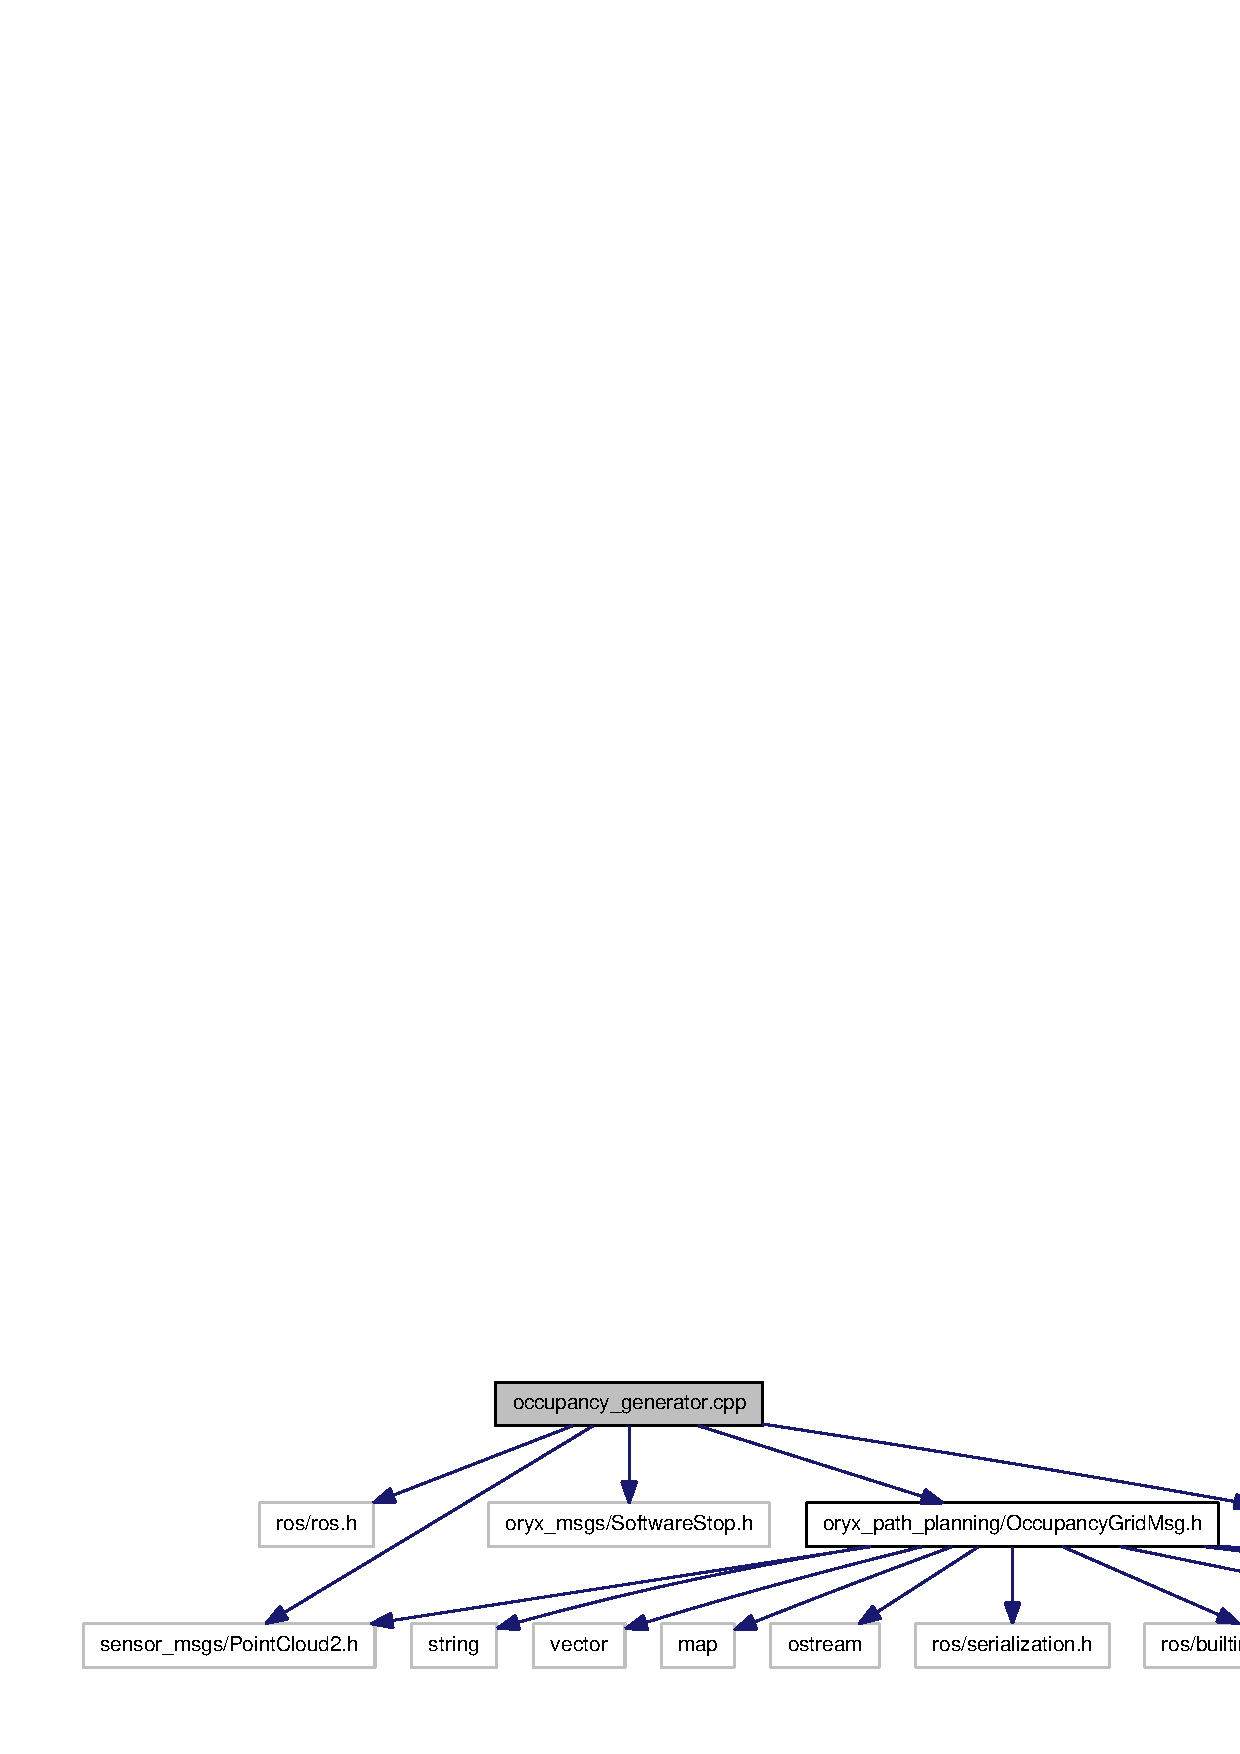
\includegraphics[width=350pt]{occupancy__generator_8cpp__incl}
\end{center}
\end{figure}
\subsection*{\-Defines}
\begin{DoxyCompactItemize}
\item 
\#define {\bf \-P\-A\-R\-A\-M\-\_\-\-W\-A\-R\-N}(param, value)~\-R\-O\-S\-\_\-\-W\-A\-R\-N(warn\-\_\-message.\-c\-\_\-str(), param.\-c\-\_\-str(), value.\-c\-\_\-str())
\begin{DoxyCompactList}\small\item\em \-Macro for printing out warning messages if default parameters are used. \end{DoxyCompactList}\end{DoxyCompactItemize}
\subsection*{\-Functions}
\begin{DoxyCompactItemize}
\item 
int {\bf main} (int argc, char $\ast$$\ast$argv)
\end{DoxyCompactItemize}


\subsection{\-Detailed \-Description}
simple node for generating test occupancy grids \begin{DoxyDate}{\-Date}
\-Oct 25, 2012 
\end{DoxyDate}
\begin{DoxyAuthor}{\-Author}
\-Adam \-Panzica 
\end{DoxyAuthor}


\-Definition in file {\bf occupancy\-\_\-generator.\-cpp}.



\subsection{\-Define \-Documentation}
\index{occupancy\-\_\-generator.\-cpp@{occupancy\-\_\-generator.\-cpp}!\-P\-A\-R\-A\-M\-\_\-\-W\-A\-R\-N@{\-P\-A\-R\-A\-M\-\_\-\-W\-A\-R\-N}}
\index{\-P\-A\-R\-A\-M\-\_\-\-W\-A\-R\-N@{\-P\-A\-R\-A\-M\-\_\-\-W\-A\-R\-N}!occupancy_generator.cpp@{occupancy\-\_\-generator.\-cpp}}
\subsubsection[{\-P\-A\-R\-A\-M\-\_\-\-W\-A\-R\-N}]{\setlength{\rightskip}{0pt plus 5cm}\#define {\bf \-P\-A\-R\-A\-M\-\_\-\-W\-A\-R\-N}(
\begin{DoxyParamCaption}
\item[{}]{param, }
\item[{}]{value}
\end{DoxyParamCaption}
)~\-R\-O\-S\-\_\-\-W\-A\-R\-N(warn\-\_\-message.\-c\-\_\-str(), param.\-c\-\_\-str(), value.\-c\-\_\-str())}\label{occupancy__generator_8cpp_a421d1715a55e4aa436fffe89c1e31248}


\-Macro for printing out warning messages if default parameters are used. 



\-Definition at line 14 of file occupancy\-\_\-generator.\-cpp.



\subsection{\-Function \-Documentation}
\index{occupancy\-\_\-generator.\-cpp@{occupancy\-\_\-generator.\-cpp}!main@{main}}
\index{main@{main}!occupancy_generator.cpp@{occupancy\-\_\-generator.\-cpp}}
\subsubsection[{main}]{\setlength{\rightskip}{0pt plus 5cm}int {\bf main} (
\begin{DoxyParamCaption}
\item[{int}]{argc, }
\item[{char $\ast$$\ast$}]{argv}
\end{DoxyParamCaption}
)}\label{occupancy__generator_8cpp_a3c04138a5bfe5d72780bb7e82a18e627}


\-Definition at line 16 of file occupancy\-\_\-generator.\-cpp.


\section{\-Occupancy\-Grid.\-cpp \-File \-Reference}
\label{OccupancyGrid_8cpp}\index{\-Occupancy\-Grid.\-cpp@{\-Occupancy\-Grid.\-cpp}}


\-Contains the implementations for \doxyref{\-Occupancy\-Grid.\-h}{p.}{OccupancyGrid_8h}.  


{\ttfamily \#include $<$boost/lexical\-\_\-cast.\-hpp$>$}\*
{\ttfamily \#include $<$tf/transform\-\_\-datatypes.\-h$>$}\*
{\ttfamily \#include $<$pcl/io/io.\-h$>$}\*
{\ttfamily \#include \char`\"{}\-Occupancy\-Grid.\-h\char`\"{}}\*
\-Include dependency graph for \-Occupancy\-Grid.\-cpp\-:
\nopagebreak
\begin{figure}[H]
\begin{center}
\leavevmode
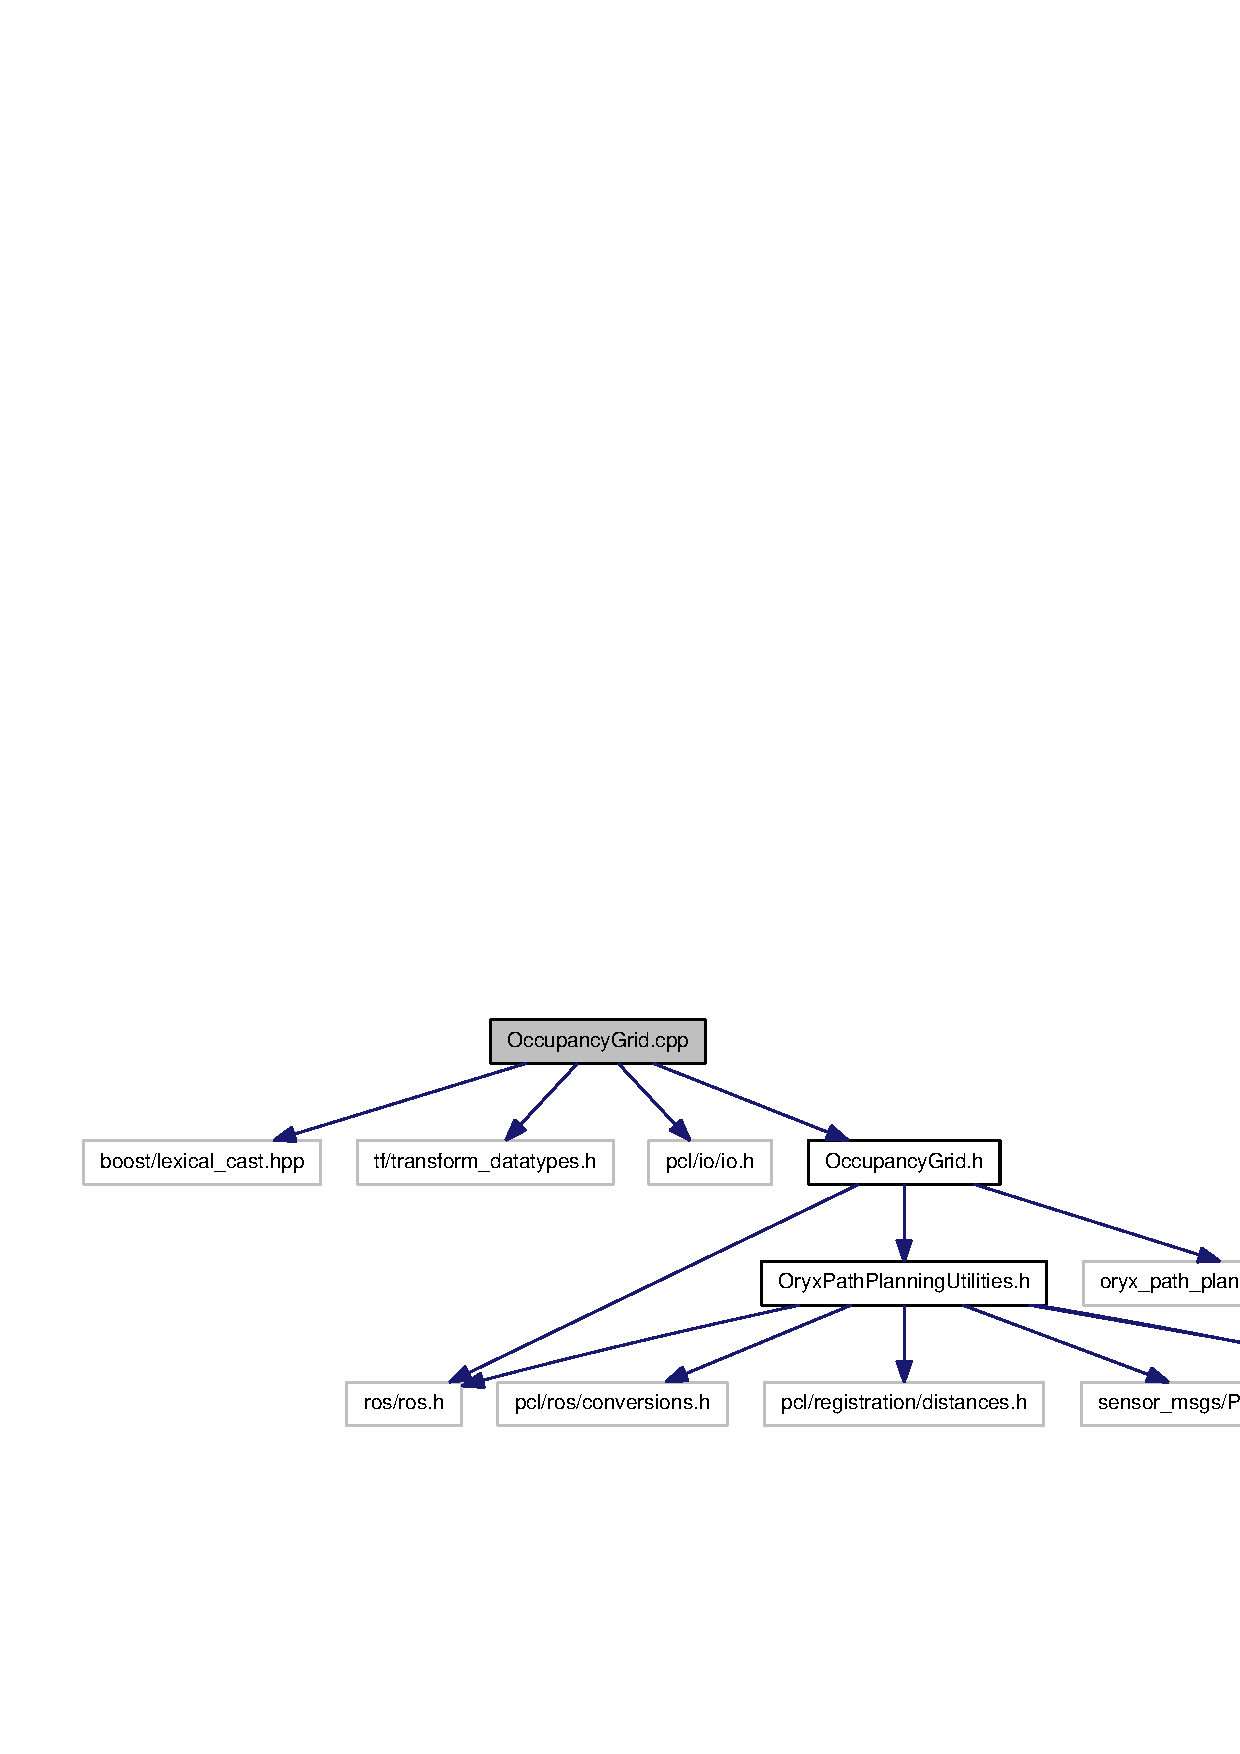
\includegraphics[width=350pt]{OccupancyGrid_8cpp__incl}
\end{center}
\end{figure}
\subsection*{\-Namespaces}
\begin{DoxyCompactItemize}
\item 
namespace {\bf oryx\-\_\-path\-\_\-planning}
\begin{DoxyCompactList}\small\item\em \-Namespace declaration to make implementation of \-Tentacle\-Traverser easier. \end{DoxyCompactList}\end{DoxyCompactItemize}


\subsection{\-Detailed \-Description}
\-Contains the implementations for \doxyref{\-Occupancy\-Grid.\-h}{p.}{OccupancyGrid_8h}. \begin{DoxyDate}{\-Date}
\-Oct 22, 2012 
\end{DoxyDate}
\begin{DoxyAuthor}{\-Author}
\-Adam \-Panzica 
\end{DoxyAuthor}


\-Definition in file {\bf \-Occupancy\-Grid.\-cpp}.


\section{\-Occupancy\-Grid.\-h \-File \-Reference}
\label{msg__gen_2cpp_2include_2oryx__path__planning_2OccupancyGrid_8h}\index{\-Occupancy\-Grid.\-h@{\-Occupancy\-Grid.\-h}}
{\ttfamily \#include $<$string$>$}\*
{\ttfamily \#include $<$vector$>$}\*
{\ttfamily \#include $<$map$>$}\*
{\ttfamily \#include $<$ostream$>$}\*
{\ttfamily \#include \char`\"{}ros/serialization.\-h\char`\"{}}\*
{\ttfamily \#include \char`\"{}ros/builtin\-\_\-message\-\_\-traits.\-h\char`\"{}}\*
{\ttfamily \#include \char`\"{}ros/message\-\_\-operations.\-h\char`\"{}}\*
{\ttfamily \#include \char`\"{}ros/time.\-h\char`\"{}}\*
{\ttfamily \#include \char`\"{}ros/macros.\-h\char`\"{}}\*
{\ttfamily \#include \char`\"{}ros/assert.\-h\char`\"{}}\*
{\ttfamily \#include \char`\"{}std\-\_\-msgs/\-Header.\-h\char`\"{}}\*
{\ttfamily \#include \char`\"{}sensor\-\_\-msgs/\-Point\-Cloud2.\-h\char`\"{}}\*
\-Include dependency graph for msg\-\_\-gen/cpp/include/oryx\-\_\-path\-\_\-planning/\-Occupancy\-Grid.h\-:
\nopagebreak
\begin{figure}[H]
\begin{center}
\leavevmode
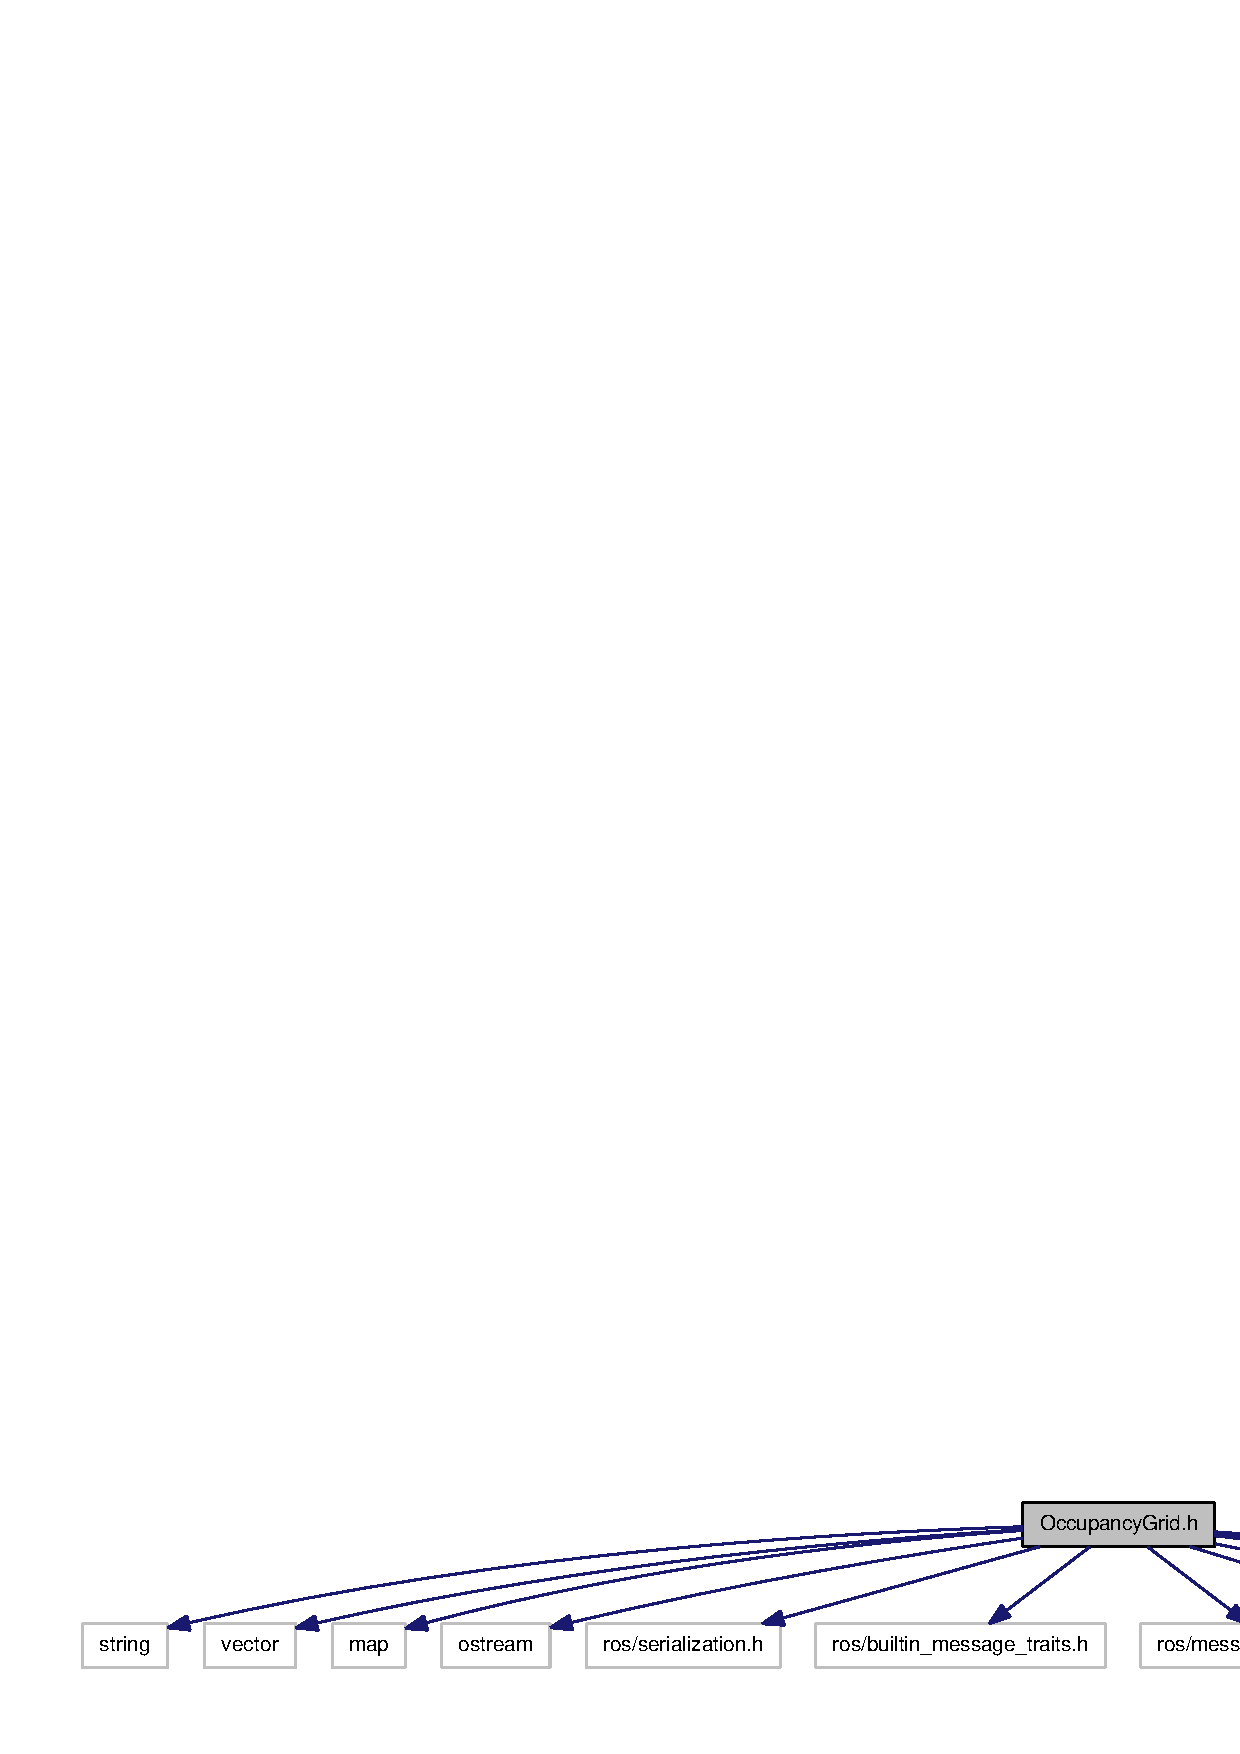
\includegraphics[width=350pt]{msg__gen_2cpp_2include_2oryx__path__planning_2OccupancyGrid_8h__incl}
\end{center}
\end{figure}
\subsection*{\-Classes}
\begin{DoxyCompactItemize}
\item 
struct {\bf ros\-::message\-\_\-traits\-::\-Data\-Type$<$ \-::oryx\-\_\-path\-\_\-planning\-::\-Occupancy\-Grid\-\_\-$<$ Container\-Allocator $>$ $>$}
\item 
struct {\bf ros\-::message\-\_\-traits\-::\-Definition$<$ \-::oryx\-\_\-path\-\_\-planning\-::\-Occupancy\-Grid\-\_\-$<$ Container\-Allocator $>$ $>$}
\item 
struct {\bf ros\-::message\-\_\-traits\-::\-Has\-Header$<$ \-::oryx\-\_\-path\-\_\-planning\-::\-Occupancy\-Grid\-\_\-$<$ Container\-Allocator $>$ $>$}
\item 
struct {\bf ros\-::message\-\_\-traits\-::\-Has\-Header$<$ const \-::oryx\-\_\-path\-\_\-planning\-::\-Occupancy\-Grid\-\_\-$<$ Container\-Allocator $>$ $>$}
\item 
struct {\bf ros\-::message\-\_\-traits\-::\-Is\-Message$<$ \-::oryx\-\_\-path\-\_\-planning\-::\-Occupancy\-Grid\-\_\-$<$ Container\-Allocator $>$ $>$}
\item 
struct {\bf ros\-::message\-\_\-traits\-::\-Is\-Message$<$ \-::oryx\-\_\-path\-\_\-planning\-::\-Occupancy\-Grid\-\_\-$<$ Container\-Allocator $>$const  $>$}
\item 
struct {\bf ros\-::message\-\_\-traits\-::\-M\-D5\-Sum$<$ \-::oryx\-\_\-path\-\_\-planning\-::\-Occupancy\-Grid\-\_\-$<$ Container\-Allocator $>$ $>$}
\item 
struct {\bf oryx\-\_\-path\-\_\-planning\-::\-Occupancy\-Grid\-\_\-$<$ Container\-Allocator $>$}
\item 
struct {\bf ros\-::message\-\_\-operations\-::\-Printer$<$ \-::oryx\-\_\-path\-\_\-planning\-::\-Occupancy\-Grid\-\_\-$<$ Container\-Allocator $>$ $>$}
\item 
struct {\bf ros\-::serialization\-::\-Serializer$<$ \-::oryx\-\_\-path\-\_\-planning\-::\-Occupancy\-Grid\-\_\-$<$ Container\-Allocator $>$ $>$}
\end{DoxyCompactItemize}
\subsection*{\-Namespaces}
\begin{DoxyCompactItemize}
\item 
namespace {\bf oryx\-\_\-path\-\_\-planning}
\begin{DoxyCompactList}\small\item\em \-Namespace declaration to make implementation of \-Tentacle\-Traverser easier. \end{DoxyCompactList}\item 
namespace {\bf ros}
\item 
namespace {\bf ros\-::message\-\_\-operations}
\item 
namespace {\bf ros\-::message\-\_\-traits}
\item 
namespace {\bf ros\-::serialization}
\end{DoxyCompactItemize}
\subsection*{\-Typedefs}
\begin{DoxyCompactItemize}
\item 
typedef \*
\-::{\bf oryx\-\_\-path\-\_\-planning\-::\-Occupancy\-Grid\-\_\-}\*
$<$ std\-::allocator$<$ void $>$ $>$ {\bf oryx\-\_\-path\-\_\-planning\-::\-Occupancy\-Grid}
\item 
typedef boost\-::shared\-\_\-ptr\*
$<$ \-::{\bf oryx\-\_\-path\-\_\-planning\-::\-Occupancy\-Grid} \*
const  $>$ {\bf oryx\-\_\-path\-\_\-planning\-::\-Occupancy\-Grid\-Const\-Ptr}
\item 
typedef boost\-::shared\-\_\-ptr\*
$<$ \-::{\bf oryx\-\_\-path\-\_\-planning\-::\-Occupancy\-Grid} $>$ {\bf oryx\-\_\-path\-\_\-planning\-::\-Occupancy\-Grid\-Ptr}
\begin{DoxyCompactList}\small\item\em \-Typedef to allow for convenient sharing of a \doxyref{\-Occupancy\-Grid}{p.}{classoryx__path__planning_1_1OccupancyGrid} via pointer. \end{DoxyCompactList}\end{DoxyCompactItemize}
\subsection*{\-Functions}
\begin{DoxyCompactItemize}
\item 
{\footnotesize template$<$typename Container\-Allocator $>$ }\\std\-::ostream \& {\bf oryx\-\_\-path\-\_\-planning\-::operator$<$$<$} (std\-::ostream \&s, const \-::{\bf oryx\-\_\-path\-\_\-planning\-::\-Occupancy\-Grid\-\_\-}$<$ \-Container\-Allocator $>$ \&v)
\end{DoxyCompactItemize}

\section{\-Occupancy\-Grid.\-h \-File \-Reference}
\label{src_2includes_2OccupancyGrid_8h}\index{\-Occupancy\-Grid.\-h@{\-Occupancy\-Grid.\-h}}
{\ttfamily \#include $<$ros/ros.\-h$>$}\*
{\ttfamily \#include \char`\"{}\-Oryx\-Path\-Planning\-Utilities.\-h\char`\"{}}\*
{\ttfamily \#include \char`\"{}oryx\-\_\-path\-\_\-planning/\-Occupancy\-Grid\-Msg.\-h\char`\"{}}\*
\-Include dependency graph for src/includes/\-Occupancy\-Grid.h\-:
\nopagebreak
\begin{figure}[H]
\begin{center}
\leavevmode
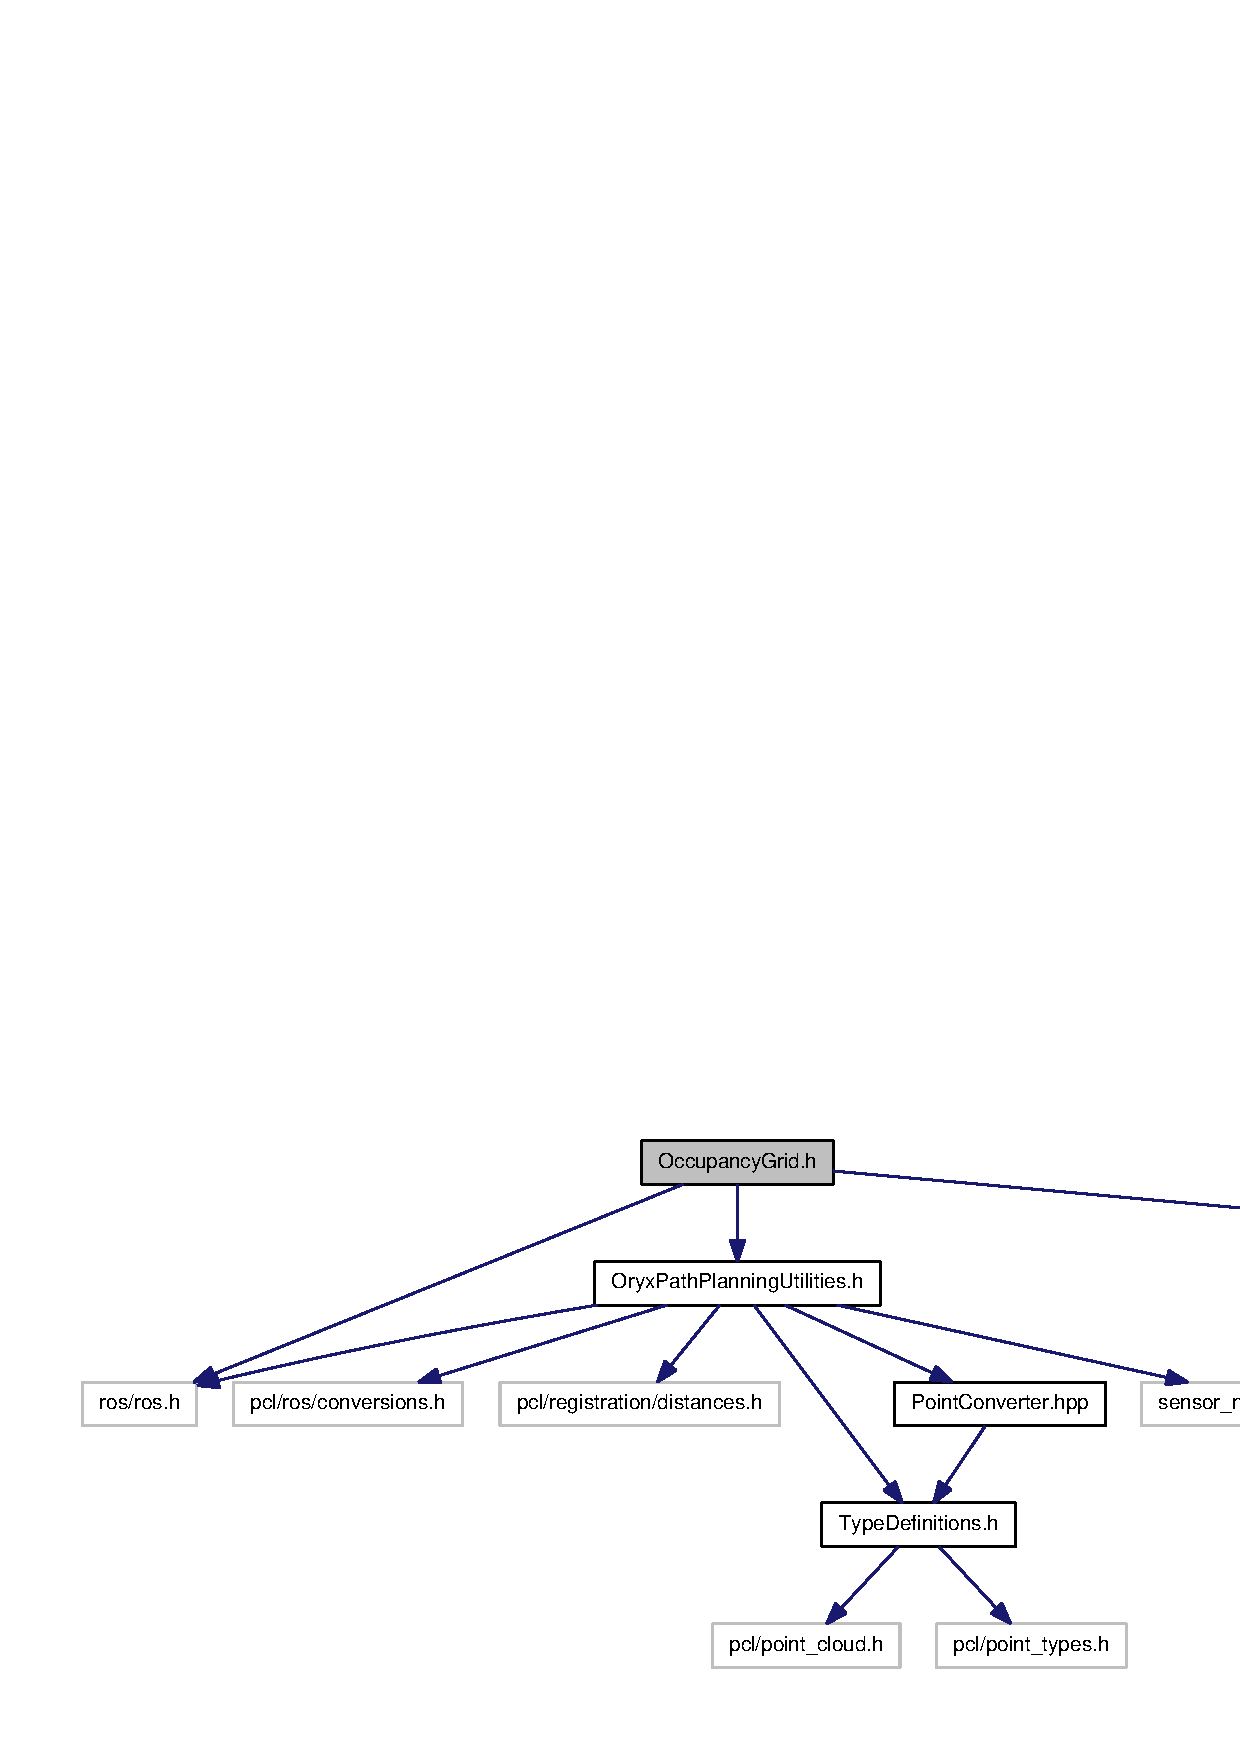
\includegraphics[width=350pt]{src_2includes_2OccupancyGrid_8h__incl}
\end{center}
\end{figure}
\-This graph shows which files directly or indirectly include this file\-:
\nopagebreak
\begin{figure}[H]
\begin{center}
\leavevmode
\includegraphics[width=350pt]{src_2includes_2OccupancyGrid_8h__dep__incl}
\end{center}
\end{figure}
\subsection*{\-Classes}
\begin{DoxyCompactItemize}
\item 
class {\bf oryx\-\_\-path\-\_\-planning\-::\-Occupancy\-Grid}
\begin{DoxyCompactList}\small\item\em \-Class which represents an \-Occupancy \-Grid that contains data on the robot's local frame. \end{DoxyCompactList}\item 
class {\bf oryx\-\_\-path\-\_\-planning\-::\-Occupancy\-Grid\-Access\-Exception}
\begin{DoxyCompactList}\small\item\em \-Basic exception for stating that an invalid location on the occupancy grid was accessed. \end{DoxyCompactList}\end{DoxyCompactItemize}
\subsection*{\-Namespaces}
\begin{DoxyCompactItemize}
\item 
namespace {\bf oryx\-\_\-path\-\_\-planning}
\begin{DoxyCompactList}\small\item\em \-Namespace declaration to make implementation of \-Tentacle\-Traverser easier. \end{DoxyCompactList}\end{DoxyCompactItemize}
\subsection*{\-Typedefs}
\begin{DoxyCompactItemize}
\item 
typedef pcl\-::\-Point\-Cloud$<$ \-Point $>$ {\bf oryx\-\_\-path\-\_\-planning\-::\-Occupancy\-Grid\-Cloud}
\end{DoxyCompactItemize}

\section{\-Occupancy\-Grid\-Msg.\-h \-File \-Reference}
\label{OccupancyGridMsg_8h}\index{\-Occupancy\-Grid\-Msg.\-h@{\-Occupancy\-Grid\-Msg.\-h}}
{\ttfamily \#include $<$string$>$}\*
{\ttfamily \#include $<$vector$>$}\*
{\ttfamily \#include $<$map$>$}\*
{\ttfamily \#include $<$ostream$>$}\*
{\ttfamily \#include \char`\"{}ros/serialization.\-h\char`\"{}}\*
{\ttfamily \#include \char`\"{}ros/builtin\-\_\-message\-\_\-traits.\-h\char`\"{}}\*
{\ttfamily \#include \char`\"{}ros/message\-\_\-operations.\-h\char`\"{}}\*
{\ttfamily \#include \char`\"{}ros/time.\-h\char`\"{}}\*
{\ttfamily \#include \char`\"{}ros/macros.\-h\char`\"{}}\*
{\ttfamily \#include \char`\"{}ros/assert.\-h\char`\"{}}\*
{\ttfamily \#include \char`\"{}std\-\_\-msgs/\-Header.\-h\char`\"{}}\*
{\ttfamily \#include \char`\"{}sensor\-\_\-msgs/\-Point\-Cloud2.\-h\char`\"{}}\*
\-Include dependency graph for \-Occupancy\-Grid\-Msg.\-h\-:
\nopagebreak
\begin{figure}[H]
\begin{center}
\leavevmode
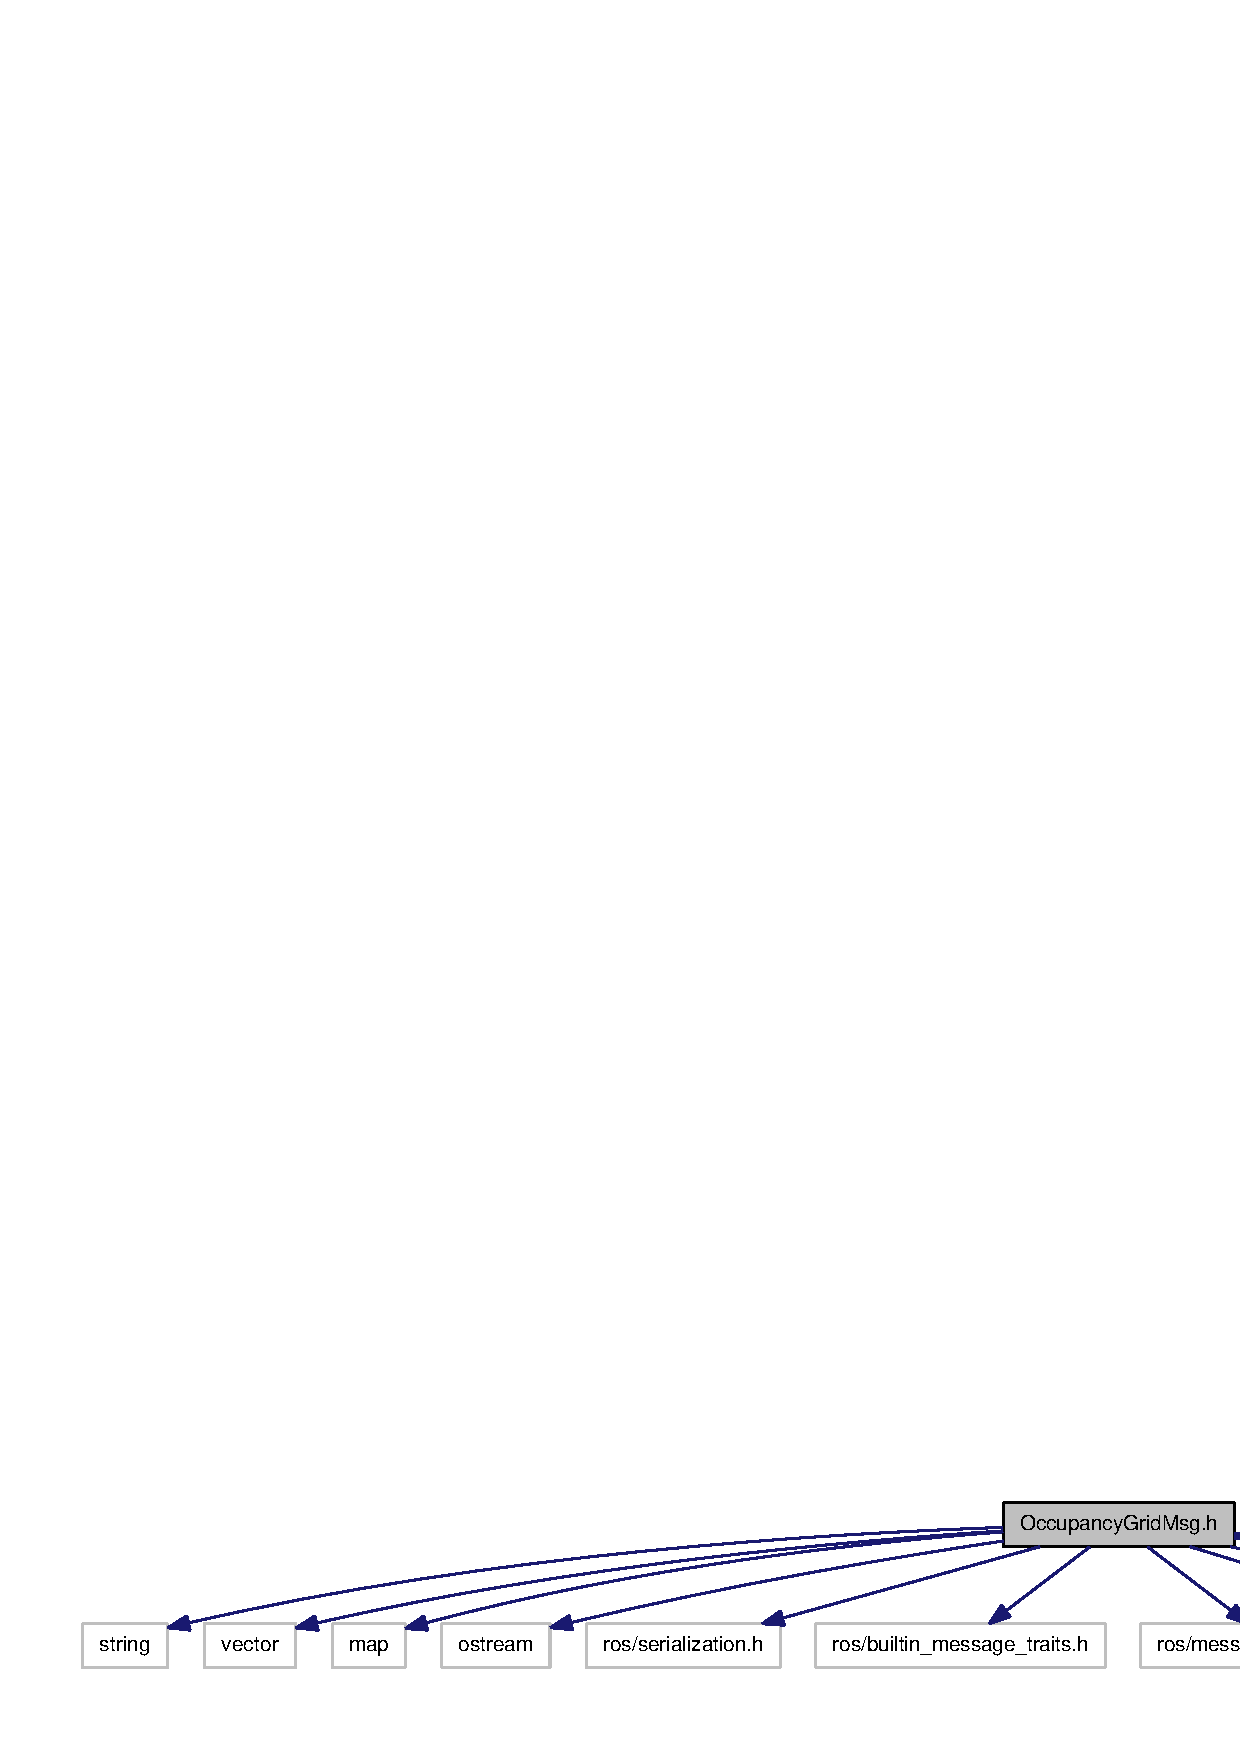
\includegraphics[width=350pt]{OccupancyGridMsg_8h__incl}
\end{center}
\end{figure}
\-This graph shows which files directly or indirectly include this file\-:
\nopagebreak
\begin{figure}[H]
\begin{center}
\leavevmode
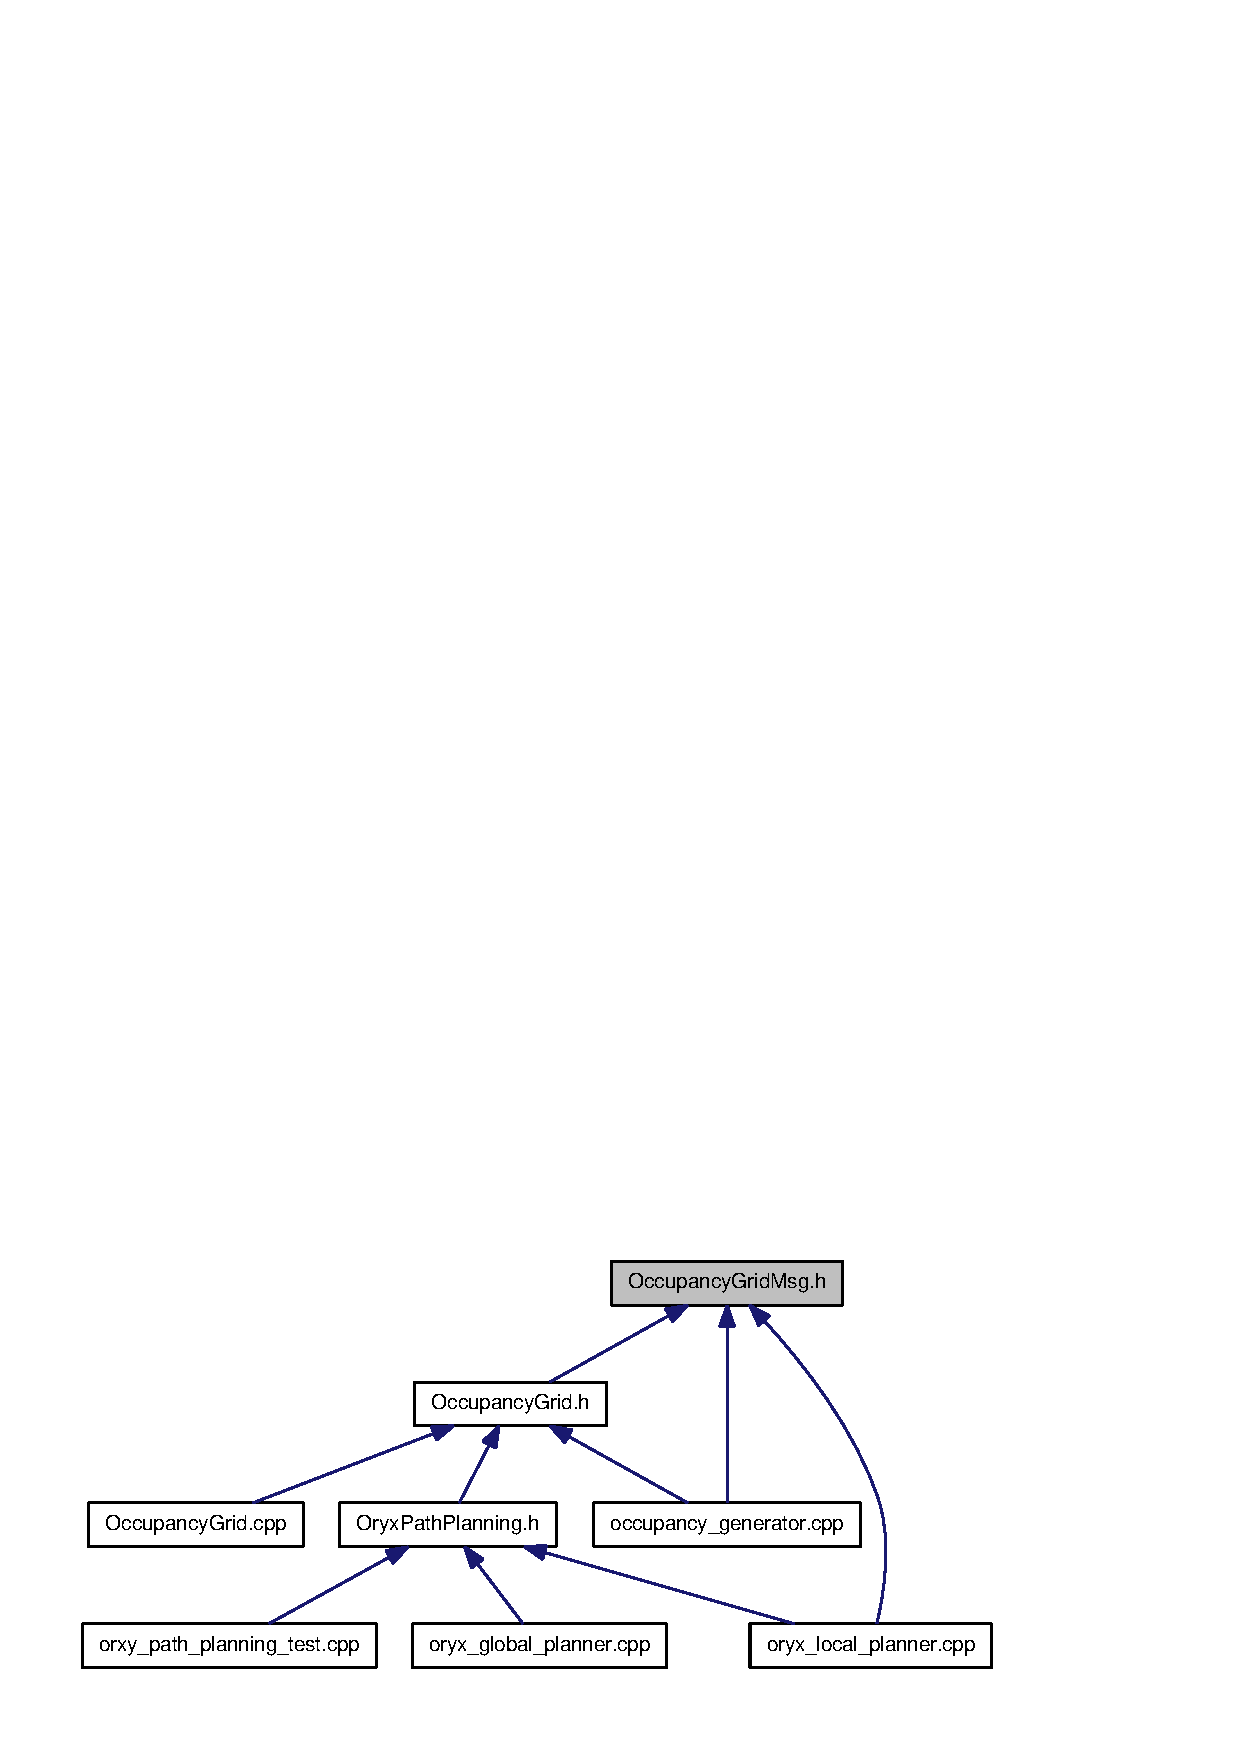
\includegraphics[width=350pt]{OccupancyGridMsg_8h__dep__incl}
\end{center}
\end{figure}
\subsection*{\-Classes}
\begin{DoxyCompactItemize}
\item 
struct {\bf ros\-::message\-\_\-traits\-::\-Data\-Type$<$ \-::oryx\-\_\-path\-\_\-planning\-::\-Occupancy\-Grid\-Msg\-\_\-$<$ Container\-Allocator $>$ $>$}
\item 
struct {\bf ros\-::message\-\_\-traits\-::\-Definition$<$ \-::oryx\-\_\-path\-\_\-planning\-::\-Occupancy\-Grid\-Msg\-\_\-$<$ Container\-Allocator $>$ $>$}
\item 
struct {\bf ros\-::message\-\_\-traits\-::\-Has\-Header$<$ \-::oryx\-\_\-path\-\_\-planning\-::\-Occupancy\-Grid\-Msg\-\_\-$<$ Container\-Allocator $>$ $>$}
\item 
struct {\bf ros\-::message\-\_\-traits\-::\-Has\-Header$<$ const \-::oryx\-\_\-path\-\_\-planning\-::\-Occupancy\-Grid\-Msg\-\_\-$<$ Container\-Allocator $>$ $>$}
\item 
struct {\bf ros\-::message\-\_\-traits\-::\-Is\-Message$<$ \-::oryx\-\_\-path\-\_\-planning\-::\-Occupancy\-Grid\-Msg\-\_\-$<$ Container\-Allocator $>$ $>$}
\item 
struct {\bf ros\-::message\-\_\-traits\-::\-Is\-Message$<$ \-::oryx\-\_\-path\-\_\-planning\-::\-Occupancy\-Grid\-Msg\-\_\-$<$ Container\-Allocator $>$const  $>$}
\item 
struct {\bf ros\-::message\-\_\-traits\-::\-M\-D5\-Sum$<$ \-::oryx\-\_\-path\-\_\-planning\-::\-Occupancy\-Grid\-Msg\-\_\-$<$ Container\-Allocator $>$ $>$}
\item 
struct {\bf oryx\-\_\-path\-\_\-planning\-::\-Occupancy\-Grid\-Msg\-\_\-$<$ Container\-Allocator $>$}
\item 
struct {\bf ros\-::message\-\_\-operations\-::\-Printer$<$ \-::oryx\-\_\-path\-\_\-planning\-::\-Occupancy\-Grid\-Msg\-\_\-$<$ Container\-Allocator $>$ $>$}
\item 
struct {\bf ros\-::serialization\-::\-Serializer$<$ \-::oryx\-\_\-path\-\_\-planning\-::\-Occupancy\-Grid\-Msg\-\_\-$<$ Container\-Allocator $>$ $>$}
\end{DoxyCompactItemize}
\subsection*{\-Namespaces}
\begin{DoxyCompactItemize}
\item 
namespace {\bf oryx\-\_\-path\-\_\-planning}
\begin{DoxyCompactList}\small\item\em \-Namespace declaration to make implementation of \-Tentacle\-Traverser easier. \end{DoxyCompactList}\item 
namespace {\bf ros}
\item 
namespace {\bf ros\-::message\-\_\-operations}
\item 
namespace {\bf ros\-::message\-\_\-traits}
\item 
namespace {\bf ros\-::serialization}
\end{DoxyCompactItemize}
\subsection*{\-Typedefs}
\begin{DoxyCompactItemize}
\item 
typedef \*
\-::{\bf oryx\-\_\-path\-\_\-planning\-::\-Occupancy\-Grid\-Msg\-\_\-}\*
$<$ std\-::allocator$<$ void $>$ $>$ {\bf oryx\-\_\-path\-\_\-planning\-::\-Occupancy\-Grid\-Msg}
\item 
typedef boost\-::shared\-\_\-ptr\*
$<$ \-::{\bf oryx\-\_\-path\-\_\-planning\-::\-Occupancy\-Grid\-Msg} \*
const  $>$ {\bf oryx\-\_\-path\-\_\-planning\-::\-Occupancy\-Grid\-Msg\-Const\-Ptr}
\item 
typedef boost\-::shared\-\_\-ptr\*
$<$ \-::{\bf oryx\-\_\-path\-\_\-planning\-::\-Occupancy\-Grid\-Msg} $>$ {\bf oryx\-\_\-path\-\_\-planning\-::\-Occupancy\-Grid\-Msg\-Ptr}
\end{DoxyCompactItemize}
\subsection*{\-Functions}
\begin{DoxyCompactItemize}
\item 
{\footnotesize template$<$typename Container\-Allocator $>$ }\\std\-::ostream \& {\bf oryx\-\_\-path\-\_\-planning\-::operator$<$$<$} (std\-::ostream \&s, const \-::{\bf oryx\-\_\-path\-\_\-planning\-::\-Occupancy\-Grid\-Msg\-\_\-}$<$ \-Container\-Allocator $>$ \&v)
\end{DoxyCompactItemize}

\section{orxy\-\_\-path\-\_\-planning\-\_\-test.\-cpp \-File \-Reference}
\label{orxy__path__planning__test_8cpp}\index{orxy\-\_\-path\-\_\-planning\-\_\-test.\-cpp@{orxy\-\_\-path\-\_\-planning\-\_\-test.\-cpp}}


\-Simple test node.  


{\ttfamily \#include $<$ros/ros.\-h$>$}\*
{\ttfamily \#include \char`\"{}\-Oryx\-Path\-Planning.\-h\char`\"{}}\*
\-Include dependency graph for orxy\-\_\-path\-\_\-planning\-\_\-test.\-cpp\-:
\nopagebreak
\begin{figure}[H]
\begin{center}
\leavevmode
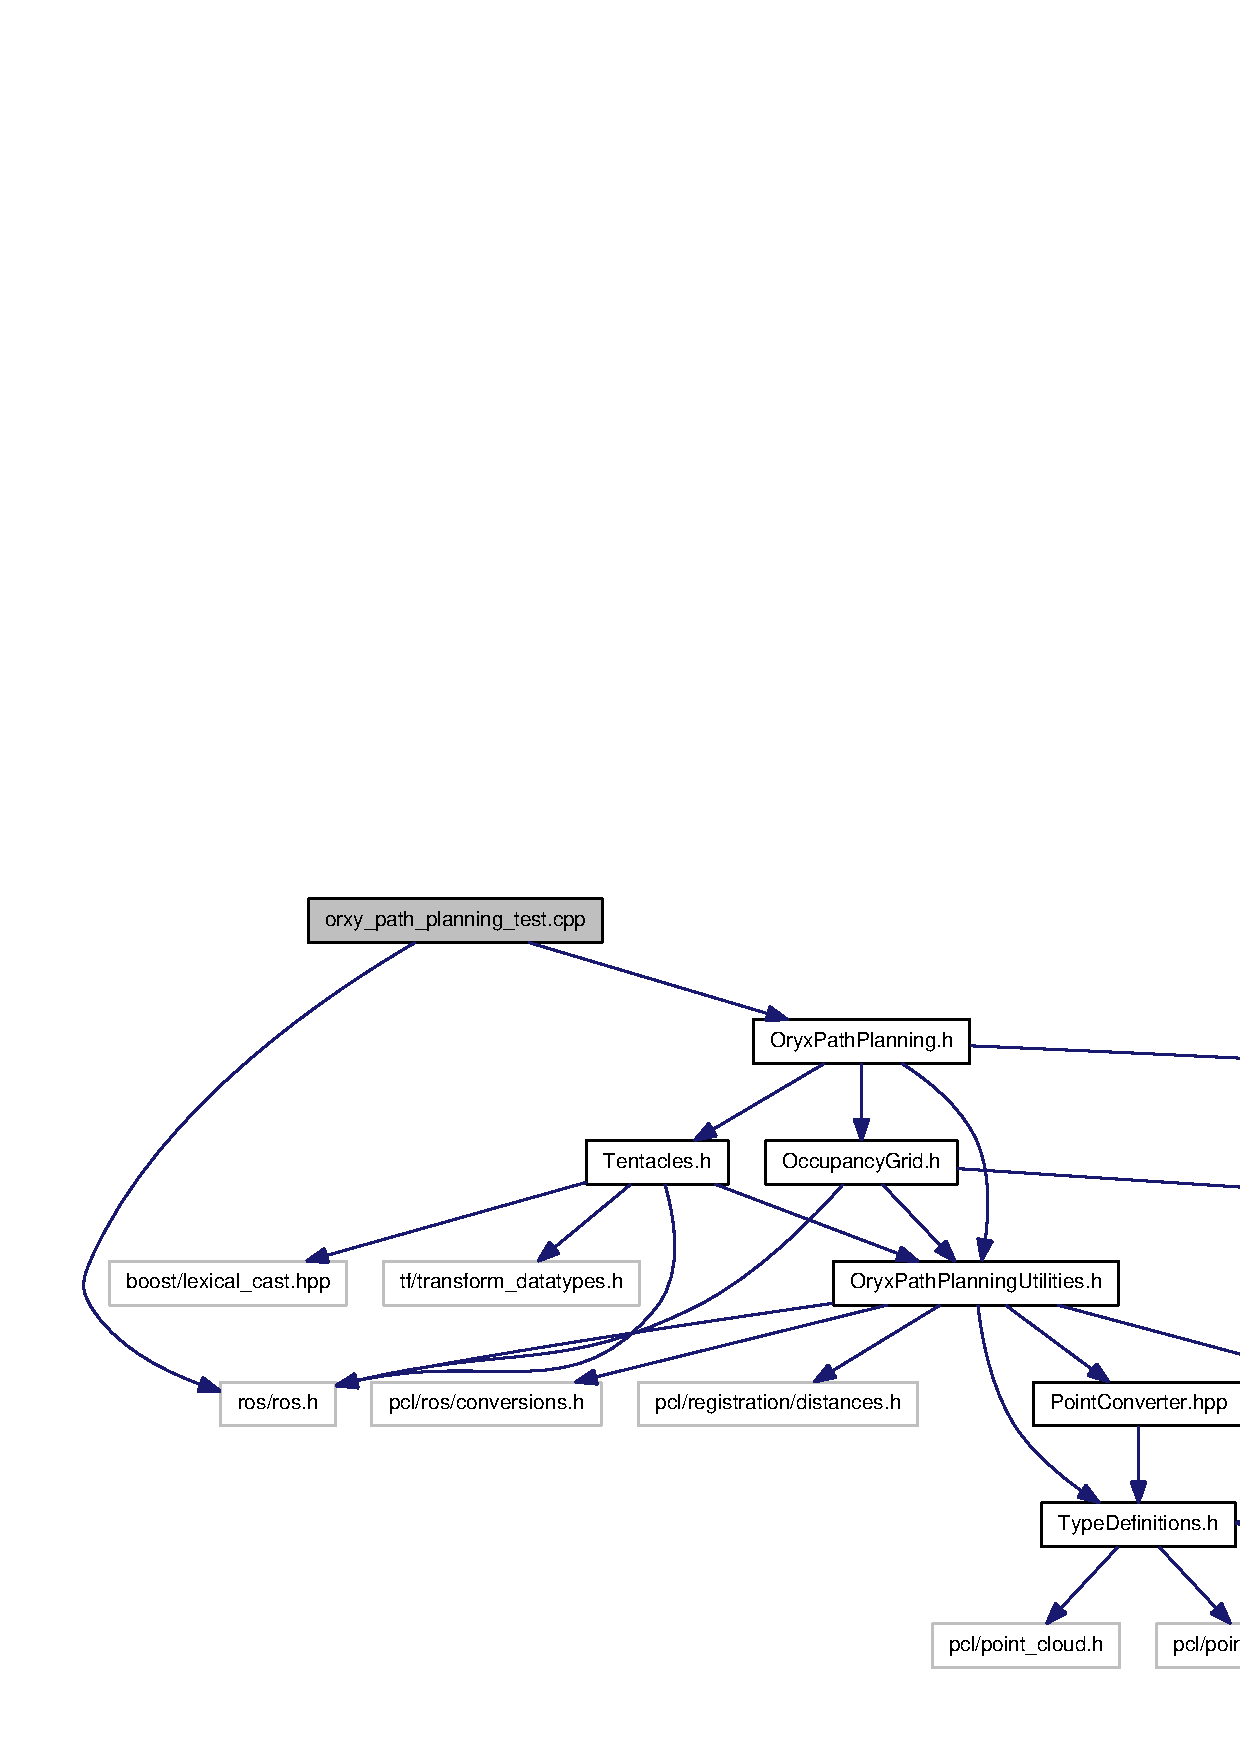
\includegraphics[width=350pt]{orxy__path__planning__test_8cpp__incl}
\end{center}
\end{figure}
\subsection*{\-Functions}
\begin{DoxyCompactItemize}
\item 
int {\bf main} (int argc, char $\ast$$\ast$argv)
\item 
void {\bf print\-Speed\-Set} (int x\-Dim, int y\-Dim, double resoltuion, {\bf \-Speed\-Set} \&speed\-Set)
\end{DoxyCompactItemize}


\subsection{\-Detailed \-Description}
\-Simple test node. \begin{DoxyDate}{\-Date}
\-Oct 11, 2012 
\end{DoxyDate}
\begin{DoxyAuthor}{\-Author}
\-Adam \-Panzica 
\end{DoxyAuthor}


\-Definition in file {\bf orxy\-\_\-path\-\_\-planning\-\_\-test.\-cpp}.



\subsection{\-Function \-Documentation}
\index{orxy\-\_\-path\-\_\-planning\-\_\-test.\-cpp@{orxy\-\_\-path\-\_\-planning\-\_\-test.\-cpp}!main@{main}}
\index{main@{main}!orxy_path_planning_test.cpp@{orxy\-\_\-path\-\_\-planning\-\_\-test.\-cpp}}
\subsubsection[{main}]{\setlength{\rightskip}{0pt plus 5cm}int {\bf main} (
\begin{DoxyParamCaption}
\item[{int}]{argc, }
\item[{char $\ast$$\ast$}]{argv}
\end{DoxyParamCaption}
)}\label{orxy__path__planning__test_8cpp_a3c04138a5bfe5d72780bb7e82a18e627}


\-Definition at line 12 of file orxy\-\_\-path\-\_\-planning\-\_\-test.\-cpp.

\index{orxy\-\_\-path\-\_\-planning\-\_\-test.\-cpp@{orxy\-\_\-path\-\_\-planning\-\_\-test.\-cpp}!print\-Speed\-Set@{print\-Speed\-Set}}
\index{print\-Speed\-Set@{print\-Speed\-Set}!orxy_path_planning_test.cpp@{orxy\-\_\-path\-\_\-planning\-\_\-test.\-cpp}}
\subsubsection[{print\-Speed\-Set}]{\setlength{\rightskip}{0pt plus 5cm}void {\bf print\-Speed\-Set} (
\begin{DoxyParamCaption}
\item[{int}]{x\-Dim, }
\item[{int}]{y\-Dim, }
\item[{double}]{resoltuion, }
\item[{{\bf \-Speed\-Set} \&}]{speed\-Set}
\end{DoxyParamCaption}
)}\label{orxy__path__planning__test_8cpp_a140f539bf966b331915c90441e9a53c3}


\-Definition at line 280 of file orxy\-\_\-path\-\_\-planning\-\_\-test.\-cpp.


\section{oryx\-\_\-global\-\_\-planner.\-cpp \-File \-Reference}
\label{oryx__global__planner_8cpp}\index{oryx\-\_\-global\-\_\-planner.\-cpp@{oryx\-\_\-global\-\_\-planner.\-cpp}}


//\-T\-O\-D\-O fill in detailed discription here  


{\ttfamily \#include $<$ros/ros.\-h$>$}\*
{\ttfamily \#include $<$boost/function.\-hpp$>$}\*
{\ttfamily \#include $<$boost/unordered\-\_\-map.\-hpp$>$}\*
{\ttfamily \#include $<$oryxsrr\-\_\-msgs/\-Command.\-h$>$}\*
{\ttfamily \#include \char`\"{}\-Oryx\-Path\-Planning.\-h\char`\"{}}\*
{\ttfamily \#include \char`\"{}\-Oryx\-Path\-Planner\-Config.\-h\char`\"{}}\*
\-Include dependency graph for oryx\-\_\-global\-\_\-planner.\-cpp\-:
\nopagebreak
\begin{figure}[H]
\begin{center}
\leavevmode
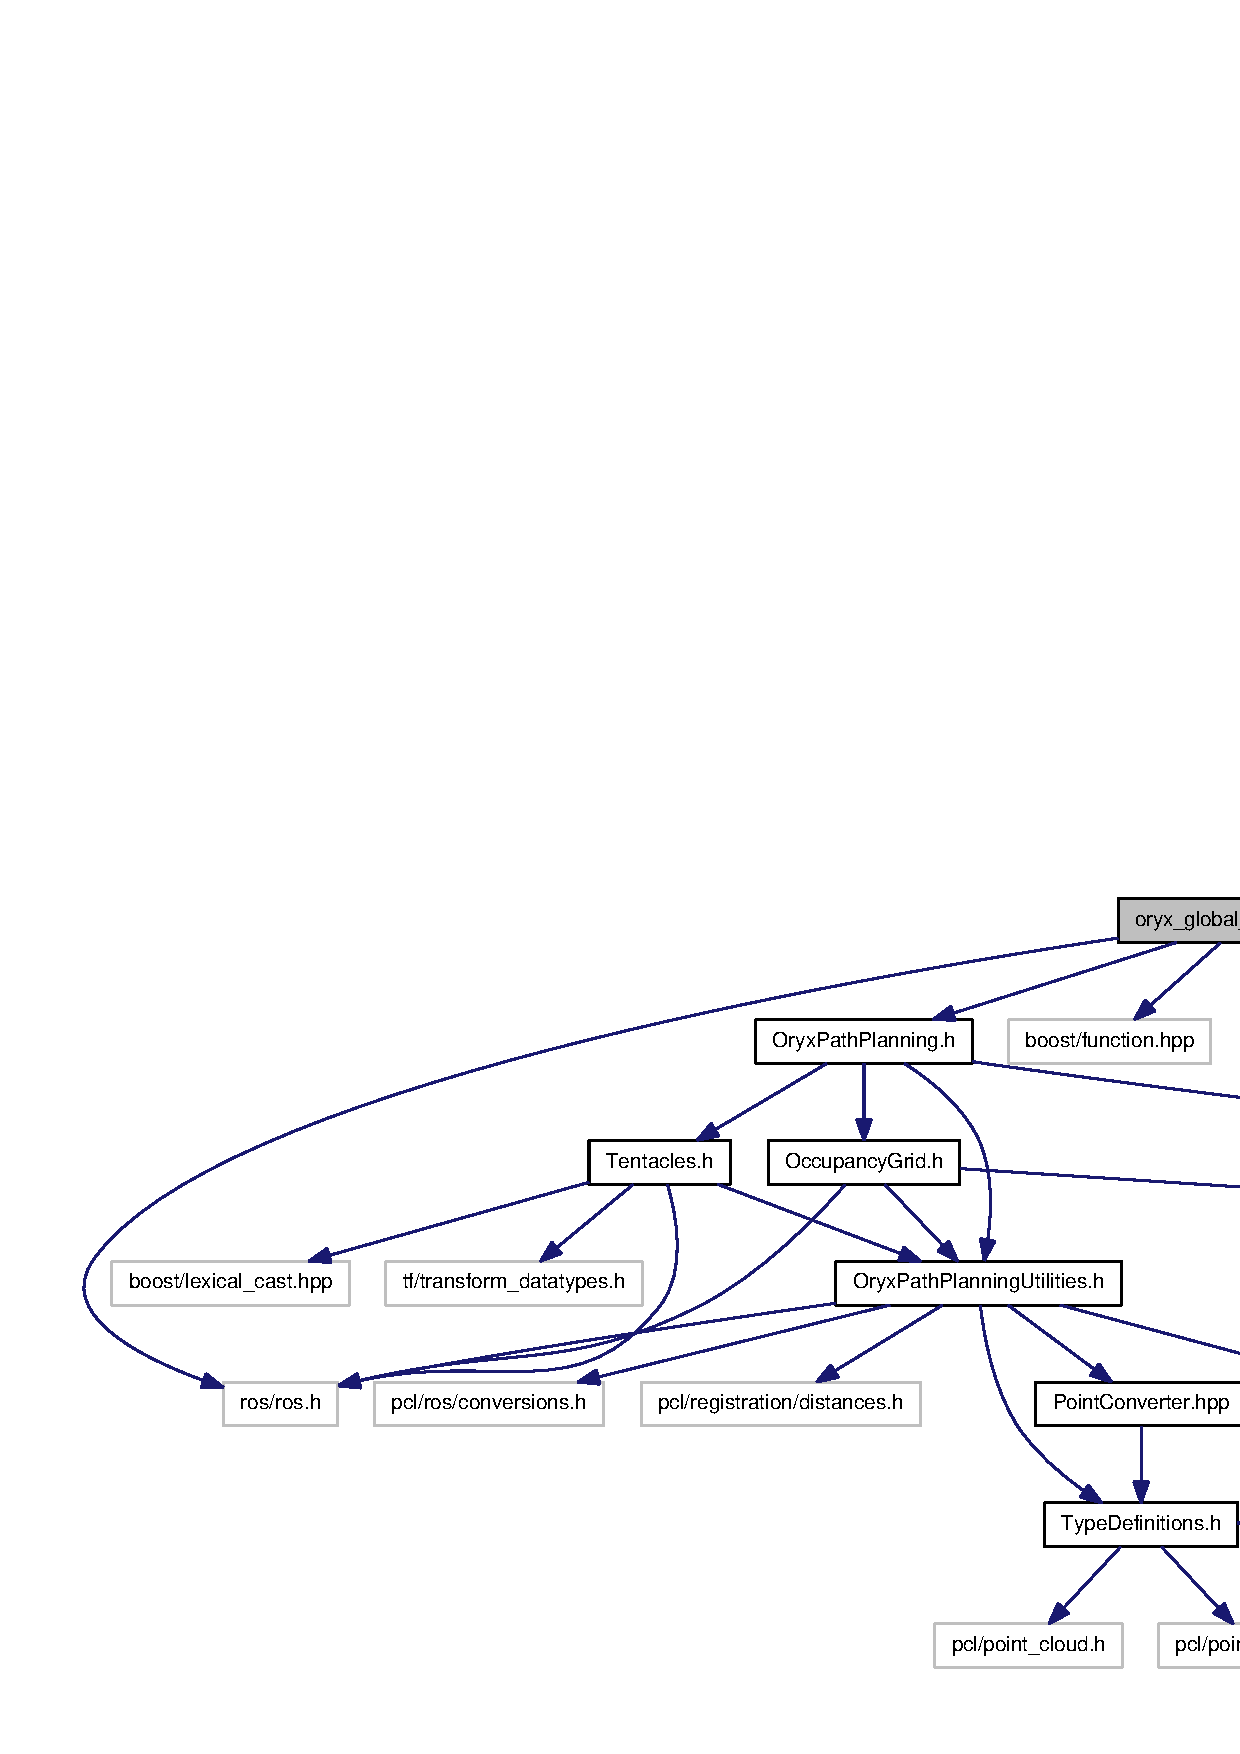
\includegraphics[width=350pt]{oryx__global__planner_8cpp__incl}
\end{center}
\end{figure}
\subsection*{\-Classes}
\begin{DoxyCompactItemize}
\item 
class {\bf \-Command\-Engine}
\begin{DoxyCompactList}\small\item\em \-Command processing engine for the global planner. \end{DoxyCompactList}\end{DoxyCompactItemize}
\subsection*{\-Functions}
\begin{DoxyCompactItemize}
\item 
int {\bf main} (int argc, char $\ast$$\ast$argv)
\end{DoxyCompactItemize}


\subsection{\-Detailed \-Description}
//\-T\-O\-D\-O fill in detailed discription here \begin{DoxyDate}{\-Date}
\-Jan 1, 2013 
\end{DoxyDate}
\begin{DoxyAuthor}{\-Author}
\-Adam \-Panzica 
\end{DoxyAuthor}


\-Definition in file {\bf oryx\-\_\-global\-\_\-planner.\-cpp}.



\subsection{\-Function \-Documentation}
\index{oryx\-\_\-global\-\_\-planner.\-cpp@{oryx\-\_\-global\-\_\-planner.\-cpp}!main@{main}}
\index{main@{main}!oryx_global_planner.cpp@{oryx\-\_\-global\-\_\-planner.\-cpp}}
\subsubsection[{main}]{\setlength{\rightskip}{0pt plus 5cm}int {\bf main} (
\begin{DoxyParamCaption}
\item[{int}]{argc, }
\item[{char $\ast$$\ast$}]{argv}
\end{DoxyParamCaption}
)}\label{oryx__global__planner_8cpp_a3c04138a5bfe5d72780bb7e82a18e627}


\-Definition at line 197 of file oryx\-\_\-global\-\_\-planner.\-cpp.


\section{oryx\-\_\-local\-\_\-planner.\-cpp \-File \-Reference}
\label{oryx__local__planner_8cpp}\index{oryx\-\_\-local\-\_\-planner.\-cpp@{oryx\-\_\-local\-\_\-planner.\-cpp}}
{\ttfamily \#include $<$queue$>$}\*
{\ttfamily \#include $<$actionlib/client/simple\-\_\-action\-\_\-client.\-h$>$}\*
{\ttfamily \#include $<$oryx\-\_\-drive\-\_\-controller/\-Velocity\-Command\-Action.\-h$>$}\*
{\ttfamily \#include $<$boost/lexical\-\_\-cast.\-hpp$>$}\*
{\ttfamily \#include $<$boost/circular\-\_\-buffer.\-hpp$>$}\*
{\ttfamily \#include $<$oryx\-\_\-msgs/\-Software\-Stop.\-h$>$}\*
{\ttfamily \#include $<$geometry\-\_\-msgs/\-Twist.\-h$>$}\*
{\ttfamily \#include \char`\"{}\-Oryx\-Path\-Planning.\-h\char`\"{}}\*
{\ttfamily \#include \char`\"{}\-Oryx\-Path\-Planner\-Config.\-h\char`\"{}}\*
{\ttfamily \#include \char`\"{}oryx\-\_\-path\-\_\-planning/\-Occupancy\-Grid\-Msg.\-h\char`\"{}}\*
\-Include dependency graph for oryx\-\_\-local\-\_\-planner.\-cpp\-:
\nopagebreak
\begin{figure}[H]
\begin{center}
\leavevmode
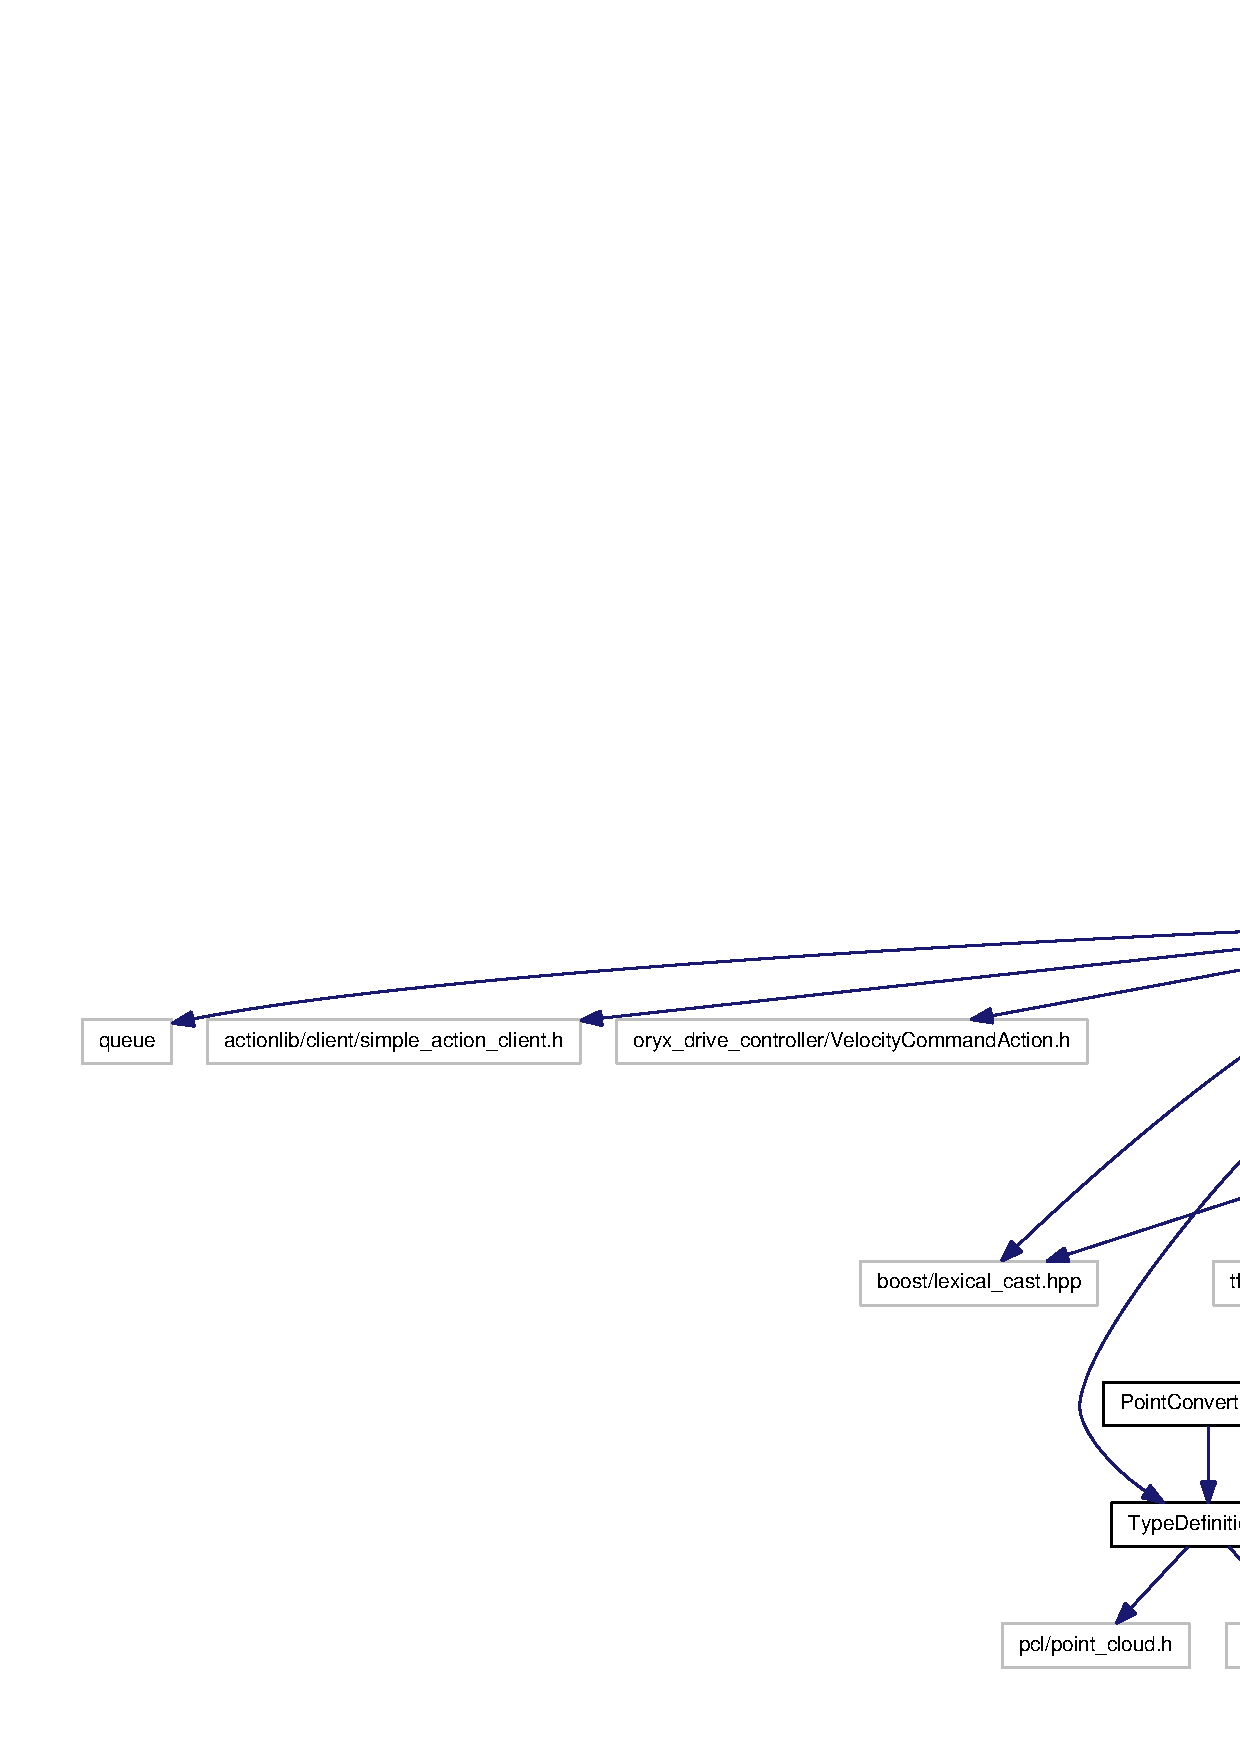
\includegraphics[width=350pt]{oryx__local__planner_8cpp__incl}
\end{center}
\end{figure}
\subsection*{\-Classes}
\begin{DoxyCompactItemize}
\item 
class {\bf \-Local\-Planner}
\begin{DoxyCompactList}\small\item\em \-Class which does the actual work of local path planning and sending commands to base. \end{DoxyCompactList}\end{DoxyCompactItemize}
\subsection*{\-Defines}
\begin{DoxyCompactItemize}
\item 
\#define {\bf \-C\-O\-N\-N\-E\-C\-T\-I\-O\-N\-\_\-\-T\-I\-M\-E\-O\-U\-T}~5.\-0
\begin{DoxyCompactList}\small\item\em \-Number of seconds to wait for connections to other \-R\-O\-S nodes before determining a system failure. \end{DoxyCompactList}\end{DoxyCompactItemize}
\subsection*{\-Functions}
\begin{DoxyCompactItemize}
\item 
int {\bf main} (int argc, char $\ast$$\ast$argv)
\end{DoxyCompactItemize}


\subsection{\-Define \-Documentation}
\index{oryx\-\_\-local\-\_\-planner.\-cpp@{oryx\-\_\-local\-\_\-planner.\-cpp}!\-C\-O\-N\-N\-E\-C\-T\-I\-O\-N\-\_\-\-T\-I\-M\-E\-O\-U\-T@{\-C\-O\-N\-N\-E\-C\-T\-I\-O\-N\-\_\-\-T\-I\-M\-E\-O\-U\-T}}
\index{\-C\-O\-N\-N\-E\-C\-T\-I\-O\-N\-\_\-\-T\-I\-M\-E\-O\-U\-T@{\-C\-O\-N\-N\-E\-C\-T\-I\-O\-N\-\_\-\-T\-I\-M\-E\-O\-U\-T}!oryx_local_planner.cpp@{oryx\-\_\-local\-\_\-planner.\-cpp}}
\subsubsection[{\-C\-O\-N\-N\-E\-C\-T\-I\-O\-N\-\_\-\-T\-I\-M\-E\-O\-U\-T}]{\setlength{\rightskip}{0pt plus 5cm}\#define {\bf \-C\-O\-N\-N\-E\-C\-T\-I\-O\-N\-\_\-\-T\-I\-M\-E\-O\-U\-T}~5.\-0}\label{oryx__local__planner_8cpp_a0c63390af22aa0f877eece67372a7414}


\-Number of seconds to wait for connections to other \-R\-O\-S nodes before determining a system failure. 



\-Definition at line 23 of file oryx\-\_\-local\-\_\-planner.\-cpp.



\subsection{\-Function \-Documentation}
\index{oryx\-\_\-local\-\_\-planner.\-cpp@{oryx\-\_\-local\-\_\-planner.\-cpp}!main@{main}}
\index{main@{main}!oryx_local_planner.cpp@{oryx\-\_\-local\-\_\-planner.\-cpp}}
\subsubsection[{main}]{\setlength{\rightskip}{0pt plus 5cm}int {\bf main} (
\begin{DoxyParamCaption}
\item[{int}]{argc, }
\item[{char $\ast$$\ast$}]{argv}
\end{DoxyParamCaption}
)}\label{oryx__local__planner_8cpp_a3c04138a5bfe5d72780bb7e82a18e627}


\-Definition at line 401 of file oryx\-\_\-local\-\_\-planner.\-cpp.


\section{\-Oryx\-Path\-Planning.\-h \-File \-Reference}
\label{OryxPathPlanning_8h}\index{\-Oryx\-Path\-Planning.\-h@{\-Oryx\-Path\-Planning.\-h}}


\-Contains all of the \-Includes required to complete the \doxyref{oryx\-\_\-path\-\_\-planning}{p.}{namespaceoryx__path__planning} namespace.  


{\ttfamily \#include \char`\"{}\-Oryx\-Path\-Planning\-Utilities.\-h\char`\"{}}\*
{\ttfamily \#include \char`\"{}\-Tentacles.\-h\char`\"{}}\*
{\ttfamily \#include \char`\"{}\-Occupancy\-Grid.\-h\char`\"{}}\*
{\ttfamily \#include \char`\"{}\-Type\-Definitions.\-h\char`\"{}}\*
\-Include dependency graph for \-Oryx\-Path\-Planning.\-h\-:
\nopagebreak
\begin{figure}[H]
\begin{center}
\leavevmode
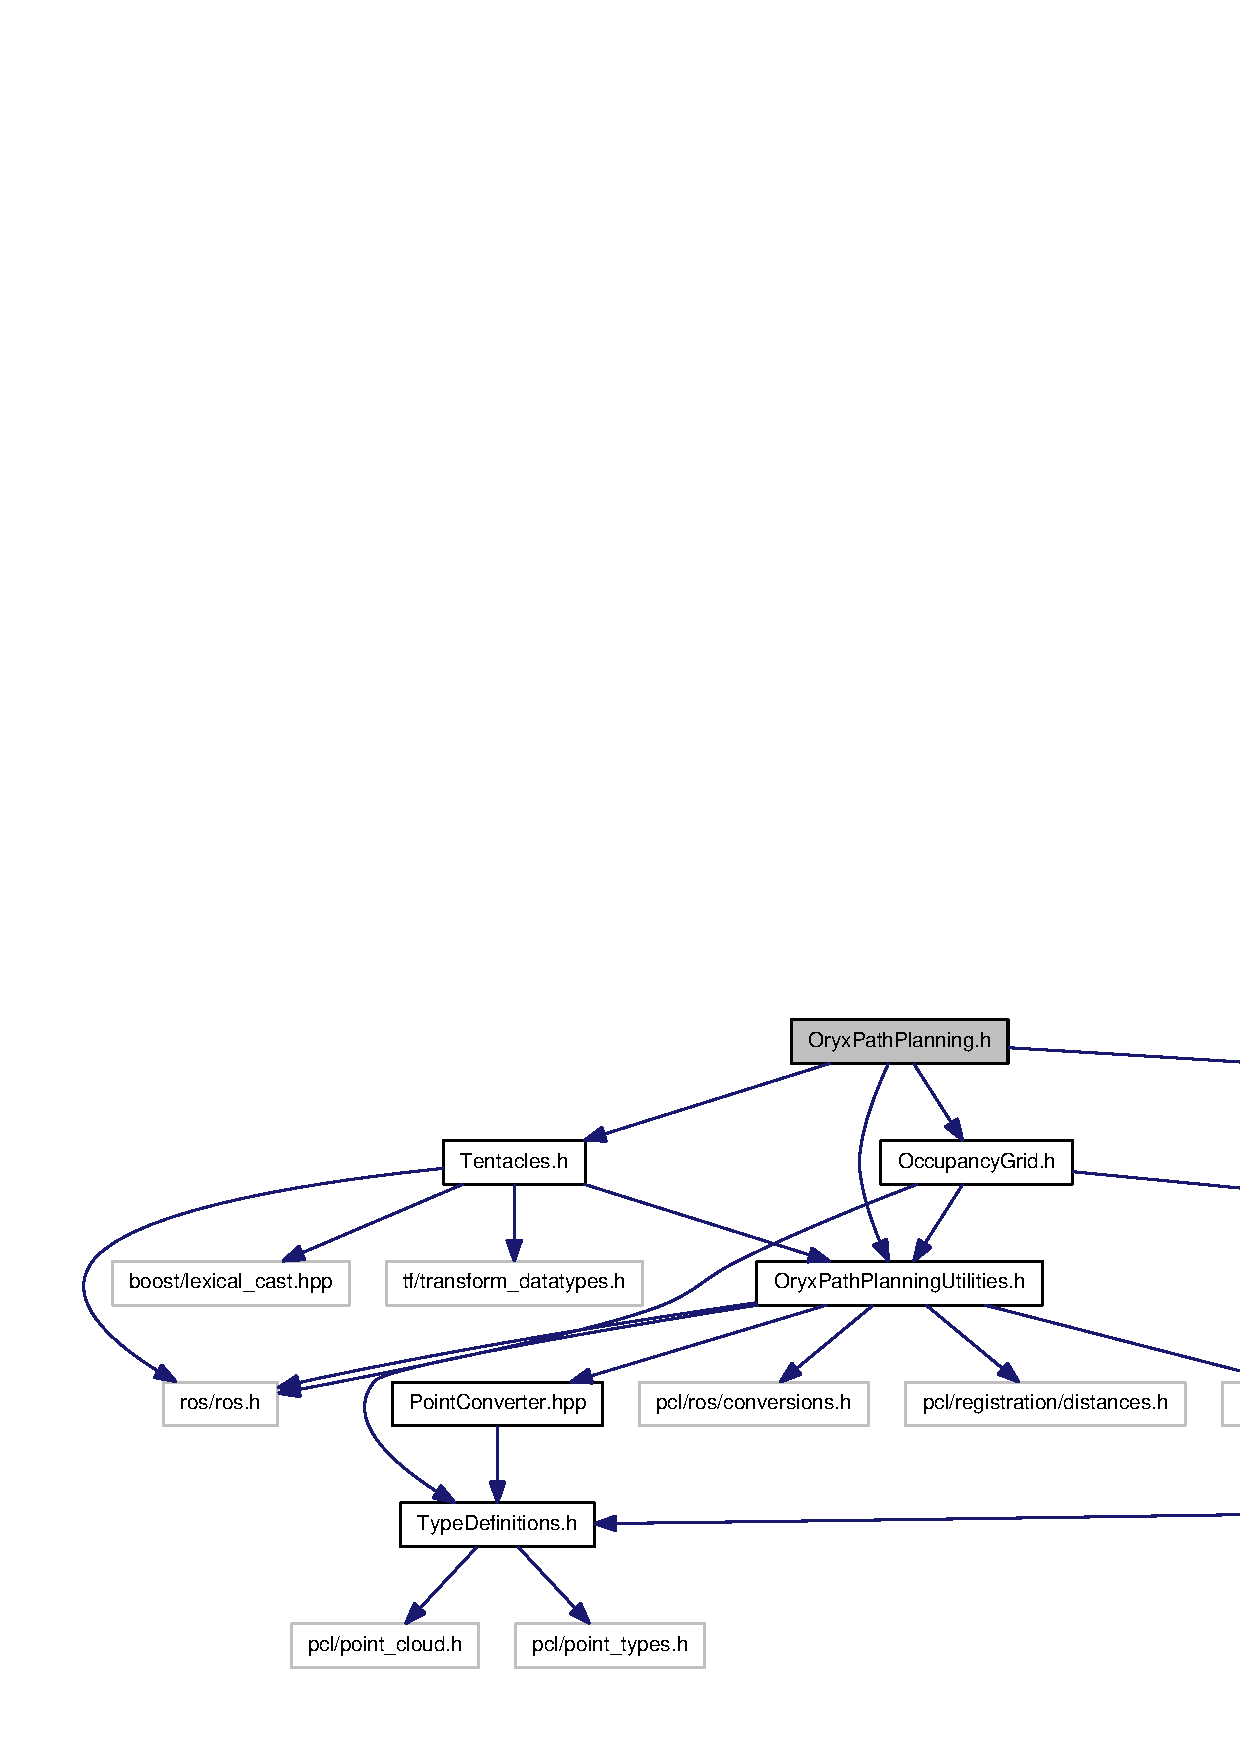
\includegraphics[width=350pt]{OryxPathPlanning_8h__incl}
\end{center}
\end{figure}
\-This graph shows which files directly or indirectly include this file\-:
\nopagebreak
\begin{figure}[H]
\begin{center}
\leavevmode
\includegraphics[width=350pt]{OryxPathPlanning_8h__dep__incl}
\end{center}
\end{figure}


\subsection{\-Detailed \-Description}
\-Contains all of the \-Includes required to complete the \doxyref{oryx\-\_\-path\-\_\-planning}{p.}{namespaceoryx__path__planning} namespace. \begin{DoxyDate}{\-Date}
\-Oct 22, 2012 
\end{DoxyDate}
\begin{DoxyAuthor}{\-Author}
\-Adam \-Panzica 
\end{DoxyAuthor}


\-Definition in file {\bf \-Oryx\-Path\-Planning.\-h}.


\section{\-Oryx\-Path\-Planning\-Utilities.\-h \-File \-Reference}
\label{OryxPathPlanningUtilities_8h}\index{\-Oryx\-Path\-Planning\-Utilities.\-h@{\-Oryx\-Path\-Planning\-Utilities.\-h}}


\-Header containing definitions that are used throughout the \doxyref{oryx\-\_\-path\-\_\-planning}{p.}{namespaceoryx__path__planning} package.  


{\ttfamily \#include $<$ros/ros.\-h$>$}\*
{\ttfamily \#include $<$pcl/ros/conversions.\-h$>$}\*
{\ttfamily \#include $<$pcl/registration/distances.\-h$>$}\*
{\ttfamily \#include $<$sensor\-\_\-msgs/\-Point\-Cloud2.\-h$>$}\*
{\ttfamily \#include \char`\"{}\-Type\-Definitions.\-h\char`\"{}}\*
{\ttfamily \#include \char`\"{}\-Point\-Converter.\-hpp\char`\"{}}\*
\-Include dependency graph for \-Oryx\-Path\-Planning\-Utilities.\-h\-:
\nopagebreak
\begin{figure}[H]
\begin{center}
\leavevmode
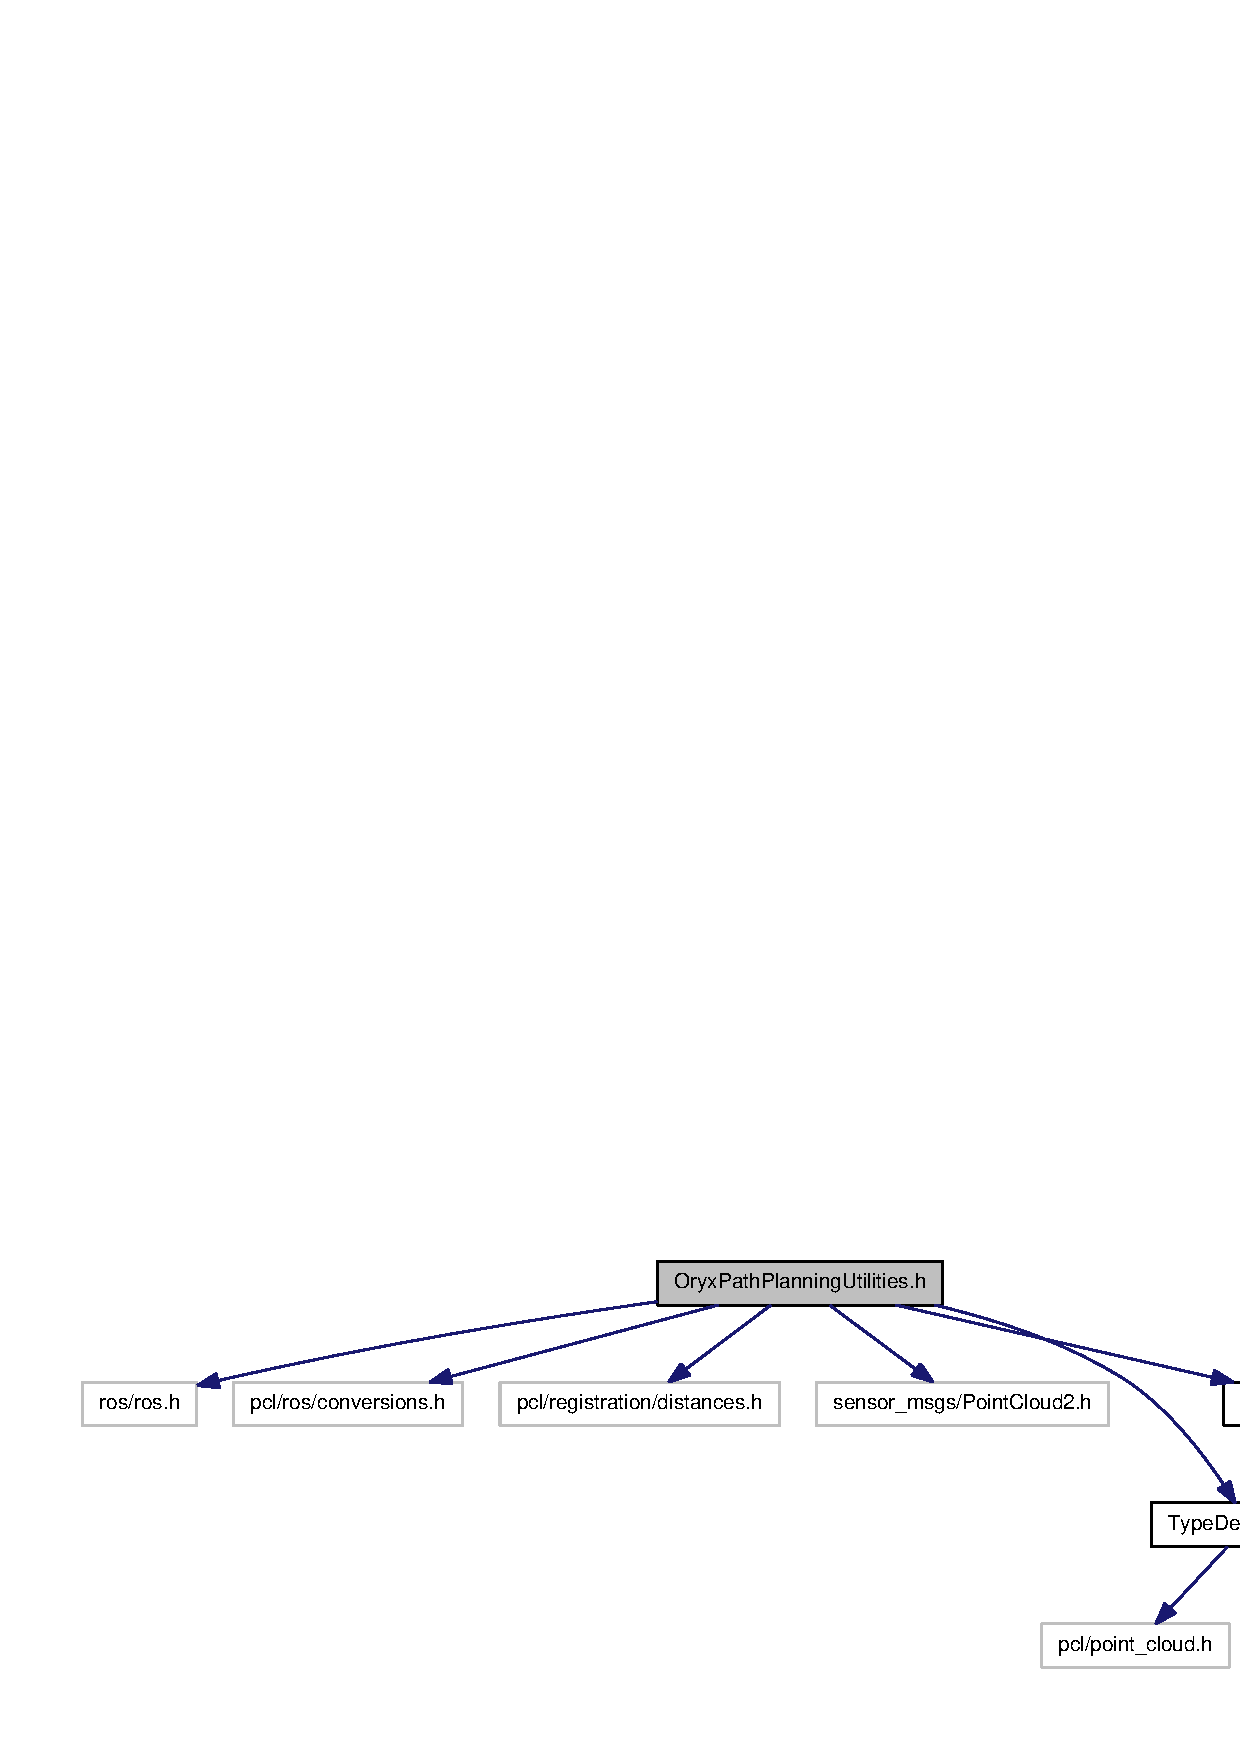
\includegraphics[width=350pt]{OryxPathPlanningUtilities_8h__incl}
\end{center}
\end{figure}
\-This graph shows which files directly or indirectly include this file\-:
\nopagebreak
\begin{figure}[H]
\begin{center}
\leavevmode
\includegraphics[width=350pt]{OryxPathPlanningUtilities_8h__dep__incl}
\end{center}
\end{figure}
\subsection*{\-Classes}
\begin{DoxyCompactItemize}
\item 
class {\bf oryx\-\_\-path\-\_\-planning\-::\-Chainable\-Exception}
\begin{DoxyCompactList}\small\item\em basic chainable exception class \end{DoxyCompactList}\item 
class {\bf oryx\-\_\-path\-\_\-planning\-::constants}
\begin{DoxyCompactList}\small\item\em singleton class which returns dynamically generated constants \end{DoxyCompactList}\end{DoxyCompactItemize}
\subsection*{\-Namespaces}
\begin{DoxyCompactItemize}
\item 
namespace {\bf oryx\-\_\-path\-\_\-planning}
\begin{DoxyCompactList}\small\item\em \-Namespace declaration to make implementation of \-Tentacle\-Traverser easier. \end{DoxyCompactList}\end{DoxyCompactItemize}
\subsection*{\-Typedefs}
\begin{DoxyCompactItemize}
\item 
typedef enum \*
{\bf oryx\-\_\-path\-\_\-planning\-::\-Point\-Trait\-\_\-t} {\bf oryx\-\_\-path\-\_\-planning\-::\-Point\-Trait}
\begin{DoxyCompactList}\small\item\em \-Standard parameter warning message. \end{DoxyCompactList}\end{DoxyCompactItemize}
\subsection*{\-Enumerations}
\begin{DoxyCompactItemize}
\item 
enum {\bf oryx\-\_\-path\-\_\-planning\-::\-Point\-Trait\-\_\-t} \{ \*
{\bf oryx\-\_\-path\-\_\-planning\-::\-O\-B\-S\-T\-A\-C\-L\-E} =  0x\-F\-F0000, 
{\bf oryx\-\_\-path\-\_\-planning\-::\-I\-N\-F\-L\-A\-T\-E\-D} =  0x0000\-F\-F, 
{\bf oryx\-\_\-path\-\_\-planning\-::\-U\-N\-K\-N\-O\-W\-N} =  0x808080, 
{\bf oryx\-\_\-path\-\_\-planning\-::\-F\-R\-E\-E\-\_\-\-H\-I\-G\-H\-\_\-\-C\-O\-S\-T} =  0x008080, 
\*
{\bf oryx\-\_\-path\-\_\-planning\-::\-F\-R\-E\-E\-\_\-\-L\-O\-W\-\_\-\-C\-O\-S\-T} =  0x008000, 
{\bf oryx\-\_\-path\-\_\-planning\-::\-T\-R\-A\-V\-E\-R\-S\-E\-D} =  0x6\-B8\-E23, 
{\bf oryx\-\_\-path\-\_\-planning\-::\-G\-O\-A\-L} =  0x\-F\-F\-F\-F00, 
{\bf oryx\-\_\-path\-\_\-planning\-::\-T\-E\-N\-T\-A\-C\-L\-E} =  0x\-C\-D00\-C\-D, 
\*
{\bf oryx\-\_\-path\-\_\-planning\-::\-R\-O\-B\-O\-T} =  0x000001
 \}
\begin{DoxyCompactList}\small\item\em \-Standard parameter warning message. \end{DoxyCompactList}\end{DoxyCompactItemize}
\subsection*{\-Functions}
\begin{DoxyCompactItemize}
\item 
void {\bf oryx\-\_\-path\-\_\-planning\-::cast\-Arc} (int radius, double sweep\-\_\-angle, int rgba, \-Point \&origin, \-Point\-Cloud \&cloud, int quadrant=1, int plane=0)
\begin{DoxyCompactList}\small\item\em \-Generates the series of points along a 90$\ast$ arc between two points and places them into a \-Point\-Cloud. \end{DoxyCompactList}\item 
void {\bf oryx\-\_\-path\-\_\-planning\-::cast\-Line} (\-Point \&start\-Point, \-Point \&end\-Point, int rgba, \-Point\-Cloud \&cloud)
\begin{DoxyCompactList}\small\item\em \-Generates the series of points along a line between two points and places them into a \-Point\-Cloud. \end{DoxyCompactList}\item 
double {\bf oryx\-\_\-path\-\_\-planning\-::grid\-To\-Real} (int grid, double resolution)
\item 
double {\bf oryx\-\_\-path\-\_\-planning\-::round\-To\-Frac} (double raw, double frac)
\item 
int {\bf oryx\-\_\-path\-\_\-planning\-::round\-To\-Grid} (double raw, double resolution)
\item 
const std\-::string {\bf oryx\-\_\-path\-\_\-planning\-::warn\-\_\-message} (\char`\"{}\-Parameter $<$\%s$>$ \-Not \-Set. \-Using \-Default \-Value $<$\%s$>$\char`\"{})
\end{DoxyCompactItemize}


\subsection{\-Detailed \-Description}
\-Header containing definitions that are used throughout the \doxyref{oryx\-\_\-path\-\_\-planning}{p.}{namespaceoryx__path__planning} package. \begin{DoxyDate}{\-Date}
\-Oct 17, 2012 
\end{DoxyDate}
\begin{DoxyAuthor}{\-Author}
\-Adam \-Panzica 
\end{DoxyAuthor}


\-Definition in file {\bf \-Oryx\-Path\-Planning\-Utilities.\-h}.


\section{\-Point\-Converter.\-hpp \-File \-Reference}
\label{PointConverter_8hpp}\index{\-Point\-Converter.\-hpp@{\-Point\-Converter.\-hpp}}


\-Header containg class definitions for converting between points.  


{\ttfamily \#include \char`\"{}\-Type\-Definitions.\-h\char`\"{}}\*
\-Include dependency graph for \-Point\-Converter.\-hpp\-:
\nopagebreak
\begin{figure}[H]
\begin{center}
\leavevmode
\includegraphics[width=242pt]{PointConverter_8hpp__incl}
\end{center}
\end{figure}
\-This graph shows which files directly or indirectly include this file\-:
\nopagebreak
\begin{figure}[H]
\begin{center}
\leavevmode
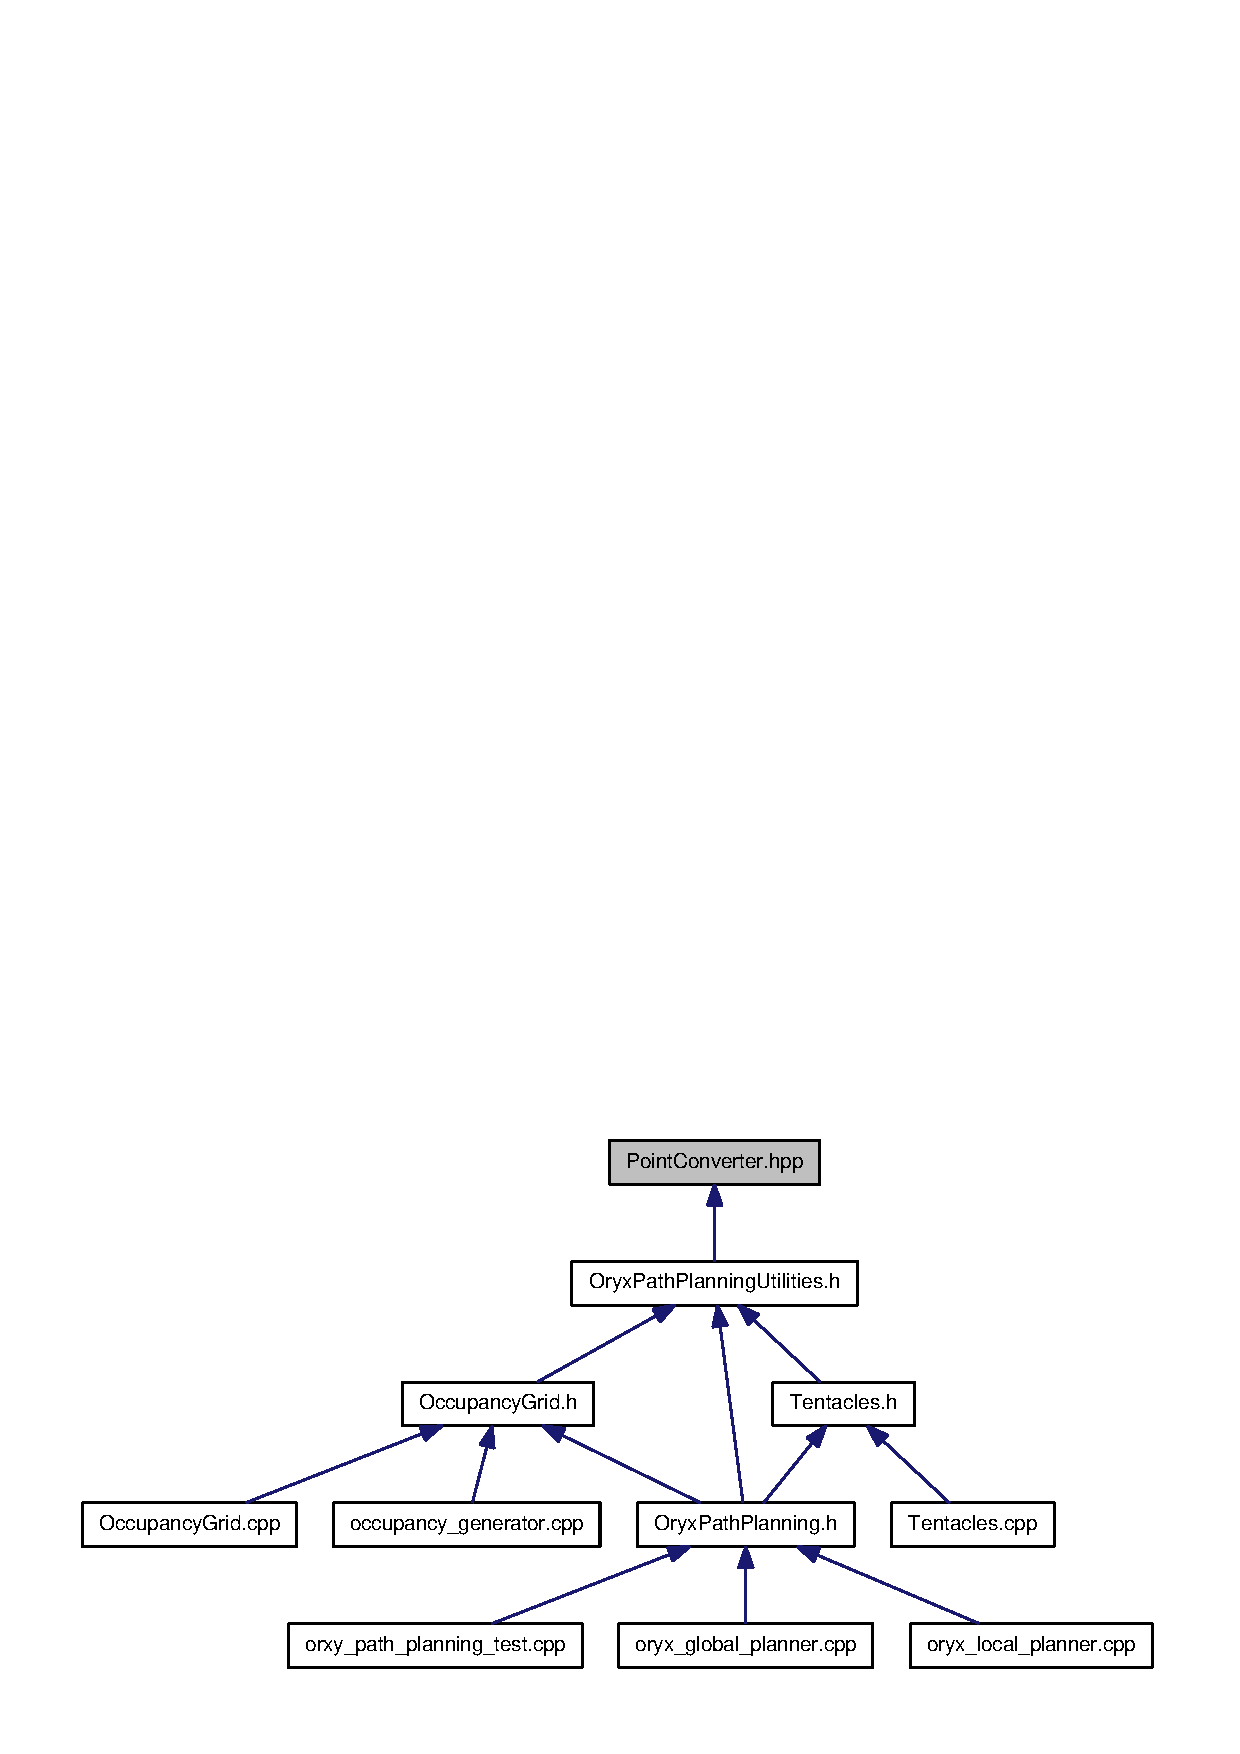
\includegraphics[width=350pt]{PointConverter_8hpp__dep__incl}
\end{center}
\end{figure}
\subsection*{\-Classes}
\begin{DoxyCompactItemize}
\item 
class {\bf oryx\-\_\-path\-\_\-planning\-::\-Point\-Converter}
\begin{DoxyCompactList}\small\item\em \-Class for converting a point with 'integer' x/y/z into some 'engineering unit' x/y/z coordinates. \end{DoxyCompactList}\end{DoxyCompactItemize}
\subsection*{\-Namespaces}
\begin{DoxyCompactItemize}
\item 
namespace {\bf oryx\-\_\-path\-\_\-planning}
\begin{DoxyCompactList}\small\item\em \-Namespace declaration to make implementation of \-Tentacle\-Traverser easier. \end{DoxyCompactList}\end{DoxyCompactItemize}


\subsection{\-Detailed \-Description}
\-Header containg class definitions for converting between points. \begin{DoxyDate}{\-Date}
\-Nov 1, 2012 
\end{DoxyDate}
\begin{DoxyAuthor}{\-Author}
\-Adam \-Panzica 
\end{DoxyAuthor}


\-Definition in file {\bf \-Point\-Converter.\-hpp}.


\section{setup.\-develspace.\-context.\-py \-File \-Reference}
\label{setup_8develspace_8context_8py}\index{setup.\-develspace.\-context.\-py@{setup.\-develspace.\-context.\-py}}
\subsection*{\-Namespaces}
\begin{DoxyCompactItemize}
\item 
namespace {\bf setup}
\end{DoxyCompactItemize}
\subsection*{\-Variables}
\begin{DoxyCompactItemize}
\item 
string {\bf setup.\-C\-A\-T\-K\-I\-N\-\_\-\-G\-L\-O\-B\-A\-L\-\_\-\-B\-I\-N\-\_\-\-D\-E\-S\-T\-I\-N\-A\-T\-I\-O\-N} = \char`\"{}bin\char`\"{}
\item 
string {\bf setup.\-C\-A\-T\-K\-I\-N\-\_\-\-G\-L\-O\-B\-A\-L\-\_\-\-L\-I\-B\-\_\-\-D\-E\-S\-T\-I\-N\-A\-T\-I\-O\-N} = \char`\"{}lib\char`\"{}
\item 
tuple {\bf setup.\-C\-M\-A\-K\-E\-\_\-\-P\-R\-E\-F\-I\-X\-\_\-\-P\-A\-T\-H} = os.\-pathsep.\-join(\char`\"{}/opt/ros/groovy\char`\"{}.split(';'))
\item 
string {\bf setup.\-P\-Y\-T\-H\-O\-N\-\_\-\-E\-X\-E\-C\-U\-T\-A\-B\-L\-E} = \char`\"{}/usr/bin/python\char`\"{}
\item 
string {\bf setup.\-P\-Y\-T\-H\-O\-N\-\_\-\-I\-N\-S\-T\-A\-L\-L\-\_\-\-D\-I\-R} = \char`\"{}lib/python2.\-7/dist-\/packages\char`\"{}
\item 
string {\bf setup.\-S\-E\-T\-U\-P\-\_\-\-D\-I\-R} = \char`\"{}/home/parallels/groovy\-\_\-workspace/oryx\-\_\-srr/oryxsrr\-\_\-msgs/devel\char`\"{}
\end{DoxyCompactItemize}

\section{setup.\-installspace.\-context.\-py \-File \-Reference}
\label{setup_8installspace_8context_8py}\index{setup.\-installspace.\-context.\-py@{setup.\-installspace.\-context.\-py}}
\subsection*{\-Namespaces}
\begin{DoxyCompactItemize}
\item 
namespace {\bf setup}
\end{DoxyCompactItemize}

\section{\-Tentacle\-\_\-test.\-cpp \-File \-Reference}
\label{Tentacle__test_8cpp}\index{\-Tentacle\-\_\-test.\-cpp@{\-Tentacle\-\_\-test.\-cpp}}
{\ttfamily \#include \char`\"{}\-Tentacle.\-h\char`\"{}}\*
\-Include dependency graph for \-Tentacle\-\_\-test.\-cpp\-:
\nopagebreak
\begin{figure}[H]
\begin{center}
\leavevmode
\includegraphics[width=138pt]{Tentacle__test_8cpp__incl}
\end{center}
\end{figure}
\subsection*{\-Namespaces}
\begin{DoxyCompactItemize}
\item 
namespace {\bf \-Translate\-Control\-Server}
\end{DoxyCompactItemize}

\section{\-Tentacles.\-cpp \-File \-Reference}
\label{Tentacles_8cpp}\index{\-Tentacles.\-cpp@{\-Tentacles.\-cpp}}
{\ttfamily \#include \char`\"{}\-Tentacles.\-h\char`\"{}}\*
{\ttfamily \#include \char`\"{}\-Oryx\-Path\-Planner\-Config.\-h\char`\"{}}\*
\-Include dependency graph for \-Tentacles.\-cpp\-:
\nopagebreak
\begin{figure}[H]
\begin{center}
\leavevmode
\includegraphics[width=350pt]{Tentacles_8cpp__incl}
\end{center}
\end{figure}
\subsection*{\-Namespaces}
\begin{DoxyCompactItemize}
\item 
namespace {\bf oryx\-\_\-path\-\_\-planning}
\begin{DoxyCompactList}\small\item\em \-Namespace declaration to make implementation of \-Tentacle\-Traverser easier. \end{DoxyCompactList}\end{DoxyCompactItemize}
\subsection*{\-Defines}
\begin{DoxyCompactItemize}
\item 
\#define {\bf \-E\-X\-P\-\_\-\-T\-E\-N\-T\-A\-C\-L\-E\-\_\-\-L\-E\-N\-G\-T\-H\-\_\-\-B\-A\-S\-E}~3.\-5
\item 
\#define {\bf \-E\-X\-P\-\_\-\-T\-E\-N\-T\-A\-C\-L\-E\-\_\-\-L\-E\-N\-G\-T\-H\-\_\-\-F\-A\-C\-T\-O\-R}~1.\-2
\item 
\#define {\bf \-M\-I\-N\-\_\-\-T\-E\-N\-T\-A\-C\-L\-E\-\_\-\-L\-E\-N\-G\-T\-H}~0.\-8
\item 
\#define {\bf \-P\-R\-I\-N\-T\-E\-R}~\-R\-O\-S\-\_\-\-D\-E\-B\-U\-G
\item 
\#define {\bf \-T\-H\-E\-T\-A\-\_\-\-I\-N\-C\-R\-E\-M\-E\-N\-T}~\-P\-I/1800.\-0
\end{DoxyCompactItemize}
\subsection*{\-Typedefs}
\begin{DoxyCompactItemize}
\item 
typedef \*
{\bf oryx\-\_\-path\-\_\-planning\-::\-Tentacle\-::\-Tentacle\-Traverser} {\bf \-Tent\-Trav}
\end{DoxyCompactItemize}


\subsection{\-Define \-Documentation}
\index{\-Tentacles.\-cpp@{\-Tentacles.\-cpp}!\-E\-X\-P\-\_\-\-T\-E\-N\-T\-A\-C\-L\-E\-\_\-\-L\-E\-N\-G\-T\-H\-\_\-\-B\-A\-S\-E@{\-E\-X\-P\-\_\-\-T\-E\-N\-T\-A\-C\-L\-E\-\_\-\-L\-E\-N\-G\-T\-H\-\_\-\-B\-A\-S\-E}}
\index{\-E\-X\-P\-\_\-\-T\-E\-N\-T\-A\-C\-L\-E\-\_\-\-L\-E\-N\-G\-T\-H\-\_\-\-B\-A\-S\-E@{\-E\-X\-P\-\_\-\-T\-E\-N\-T\-A\-C\-L\-E\-\_\-\-L\-E\-N\-G\-T\-H\-\_\-\-B\-A\-S\-E}!Tentacles.cpp@{\-Tentacles.\-cpp}}
\subsubsection[{\-E\-X\-P\-\_\-\-T\-E\-N\-T\-A\-C\-L\-E\-\_\-\-L\-E\-N\-G\-T\-H\-\_\-\-B\-A\-S\-E}]{\setlength{\rightskip}{0pt plus 5cm}\#define {\bf \-E\-X\-P\-\_\-\-T\-E\-N\-T\-A\-C\-L\-E\-\_\-\-L\-E\-N\-G\-T\-H\-\_\-\-B\-A\-S\-E}~3.\-5}\label{Tentacles_8cpp_ae129e318880d6c255dd690fd05c56eb0}


\-Definition at line 26 of file \-Tentacles.\-cpp.

\index{\-Tentacles.\-cpp@{\-Tentacles.\-cpp}!\-E\-X\-P\-\_\-\-T\-E\-N\-T\-A\-C\-L\-E\-\_\-\-L\-E\-N\-G\-T\-H\-\_\-\-F\-A\-C\-T\-O\-R@{\-E\-X\-P\-\_\-\-T\-E\-N\-T\-A\-C\-L\-E\-\_\-\-L\-E\-N\-G\-T\-H\-\_\-\-F\-A\-C\-T\-O\-R}}
\index{\-E\-X\-P\-\_\-\-T\-E\-N\-T\-A\-C\-L\-E\-\_\-\-L\-E\-N\-G\-T\-H\-\_\-\-F\-A\-C\-T\-O\-R@{\-E\-X\-P\-\_\-\-T\-E\-N\-T\-A\-C\-L\-E\-\_\-\-L\-E\-N\-G\-T\-H\-\_\-\-F\-A\-C\-T\-O\-R}!Tentacles.cpp@{\-Tentacles.\-cpp}}
\subsubsection[{\-E\-X\-P\-\_\-\-T\-E\-N\-T\-A\-C\-L\-E\-\_\-\-L\-E\-N\-G\-T\-H\-\_\-\-F\-A\-C\-T\-O\-R}]{\setlength{\rightskip}{0pt plus 5cm}\#define {\bf \-E\-X\-P\-\_\-\-T\-E\-N\-T\-A\-C\-L\-E\-\_\-\-L\-E\-N\-G\-T\-H\-\_\-\-F\-A\-C\-T\-O\-R}~1.\-2}\label{Tentacles_8cpp_a469fe07996a3cecca30dcc9bacdb6a52}


\-Definition at line 32 of file \-Tentacles.\-cpp.

\index{\-Tentacles.\-cpp@{\-Tentacles.\-cpp}!\-M\-I\-N\-\_\-\-T\-E\-N\-T\-A\-C\-L\-E\-\_\-\-L\-E\-N\-G\-T\-H@{\-M\-I\-N\-\_\-\-T\-E\-N\-T\-A\-C\-L\-E\-\_\-\-L\-E\-N\-G\-T\-H}}
\index{\-M\-I\-N\-\_\-\-T\-E\-N\-T\-A\-C\-L\-E\-\_\-\-L\-E\-N\-G\-T\-H@{\-M\-I\-N\-\_\-\-T\-E\-N\-T\-A\-C\-L\-E\-\_\-\-L\-E\-N\-G\-T\-H}!Tentacles.cpp@{\-Tentacles.\-cpp}}
\subsubsection[{\-M\-I\-N\-\_\-\-T\-E\-N\-T\-A\-C\-L\-E\-\_\-\-L\-E\-N\-G\-T\-H}]{\setlength{\rightskip}{0pt plus 5cm}\#define {\bf \-M\-I\-N\-\_\-\-T\-E\-N\-T\-A\-C\-L\-E\-\_\-\-L\-E\-N\-G\-T\-H}~0.\-8}\label{Tentacles_8cpp_a9665ead32ec6ee199b8149acce7eaec7}


\-Definition at line 20 of file \-Tentacles.\-cpp.

\index{\-Tentacles.\-cpp@{\-Tentacles.\-cpp}!\-P\-R\-I\-N\-T\-E\-R@{\-P\-R\-I\-N\-T\-E\-R}}
\index{\-P\-R\-I\-N\-T\-E\-R@{\-P\-R\-I\-N\-T\-E\-R}!Tentacles.cpp@{\-Tentacles.\-cpp}}
\subsubsection[{\-P\-R\-I\-N\-T\-E\-R}]{\setlength{\rightskip}{0pt plus 5cm}\#define {\bf \-P\-R\-I\-N\-T\-E\-R}~\-R\-O\-S\-\_\-\-D\-E\-B\-U\-G}\label{Tentacles_8cpp_a15ef04095568844ee28ee56191c9d903}


\-Definition at line 16 of file \-Tentacles.\-cpp.

\index{\-Tentacles.\-cpp@{\-Tentacles.\-cpp}!\-T\-H\-E\-T\-A\-\_\-\-I\-N\-C\-R\-E\-M\-E\-N\-T@{\-T\-H\-E\-T\-A\-\_\-\-I\-N\-C\-R\-E\-M\-E\-N\-T}}
\index{\-T\-H\-E\-T\-A\-\_\-\-I\-N\-C\-R\-E\-M\-E\-N\-T@{\-T\-H\-E\-T\-A\-\_\-\-I\-N\-C\-R\-E\-M\-E\-N\-T}!Tentacles.cpp@{\-Tentacles.\-cpp}}
\subsubsection[{\-T\-H\-E\-T\-A\-\_\-\-I\-N\-C\-R\-E\-M\-E\-N\-T}]{\setlength{\rightskip}{0pt plus 5cm}\#define {\bf \-T\-H\-E\-T\-A\-\_\-\-I\-N\-C\-R\-E\-M\-E\-N\-T}~\-P\-I/1800.\-0}\label{Tentacles_8cpp_a7b093b9bf7eacfe3d379569d3672e661}


\-Definition at line 38 of file \-Tentacles.\-cpp.



\subsection{\-Typedef \-Documentation}
\index{\-Tentacles.\-cpp@{\-Tentacles.\-cpp}!\-Tent\-Trav@{\-Tent\-Trav}}
\index{\-Tent\-Trav@{\-Tent\-Trav}!Tentacles.cpp@{\-Tentacles.\-cpp}}
\subsubsection[{\-Tent\-Trav}]{\setlength{\rightskip}{0pt plus 5cm}typedef {\bf oryx\-\_\-path\-\_\-planning\-::\-Tentacle\-::\-Tentacle\-Traverser} {\bf \-Tent\-Trav}}\label{Tentacles_8cpp_a9fce116c4dc10629707fc8e057e235a1}


\-Definition at line 45 of file \-Tentacles.\-cpp.


\section{\-Tentacles.\-h \-File \-Reference}
\label{Tentacles_8h}\index{\-Tentacles.\-h@{\-Tentacles.\-h}}
{\ttfamily \#include $<$ros/ros.\-h$>$}\*
{\ttfamily \#include $<$boost/lexical\-\_\-cast.\-hpp$>$}\*
{\ttfamily \#include $<$tf/transform\-\_\-datatypes.\-h$>$}\*
{\ttfamily \#include \char`\"{}\-Oryx\-Path\-Planning\-Utilities.\-h\char`\"{}}\*
\-Include dependency graph for \-Tentacles.\-h\-:
\nopagebreak
\begin{figure}[H]
\begin{center}
\leavevmode
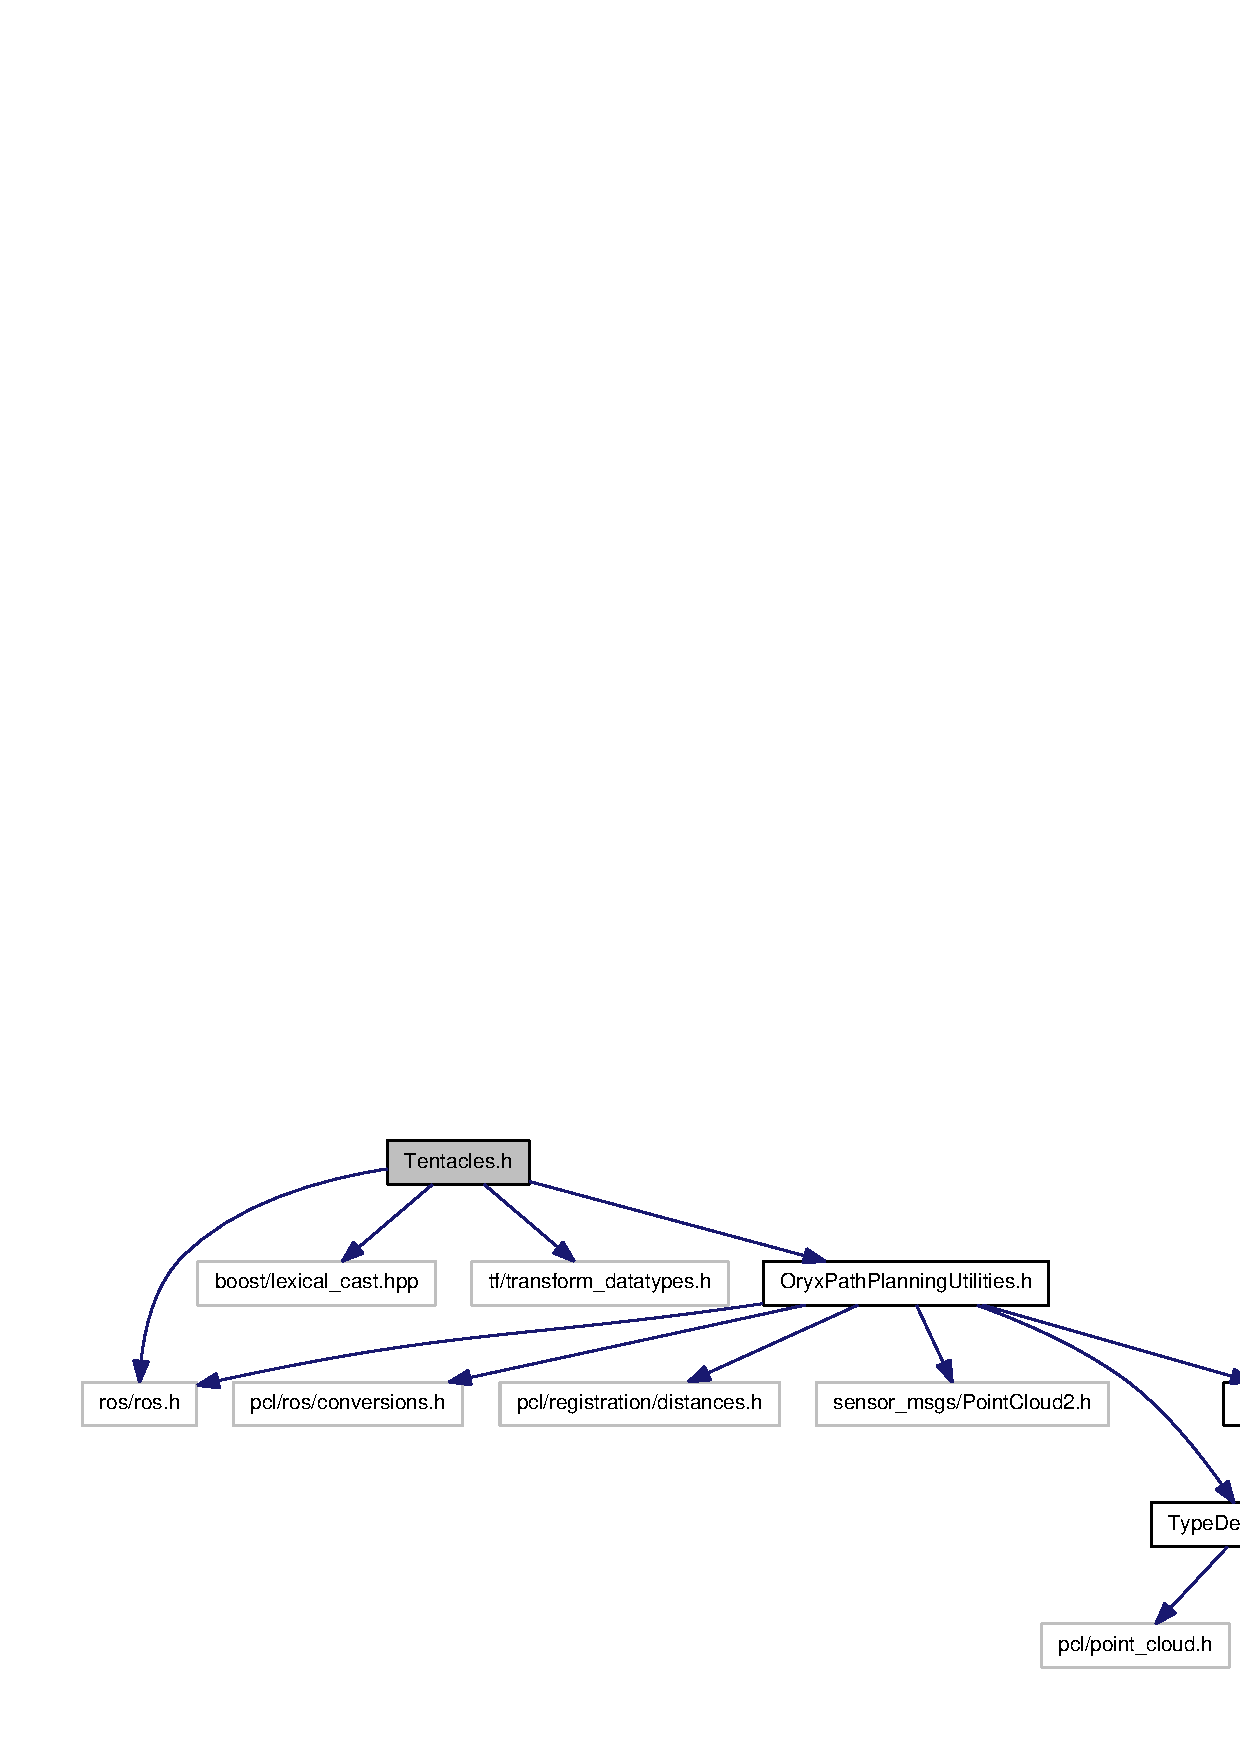
\includegraphics[width=350pt]{Tentacles_8h__incl}
\end{center}
\end{figure}
\-This graph shows which files directly or indirectly include this file\-:
\nopagebreak
\begin{figure}[H]
\begin{center}
\leavevmode
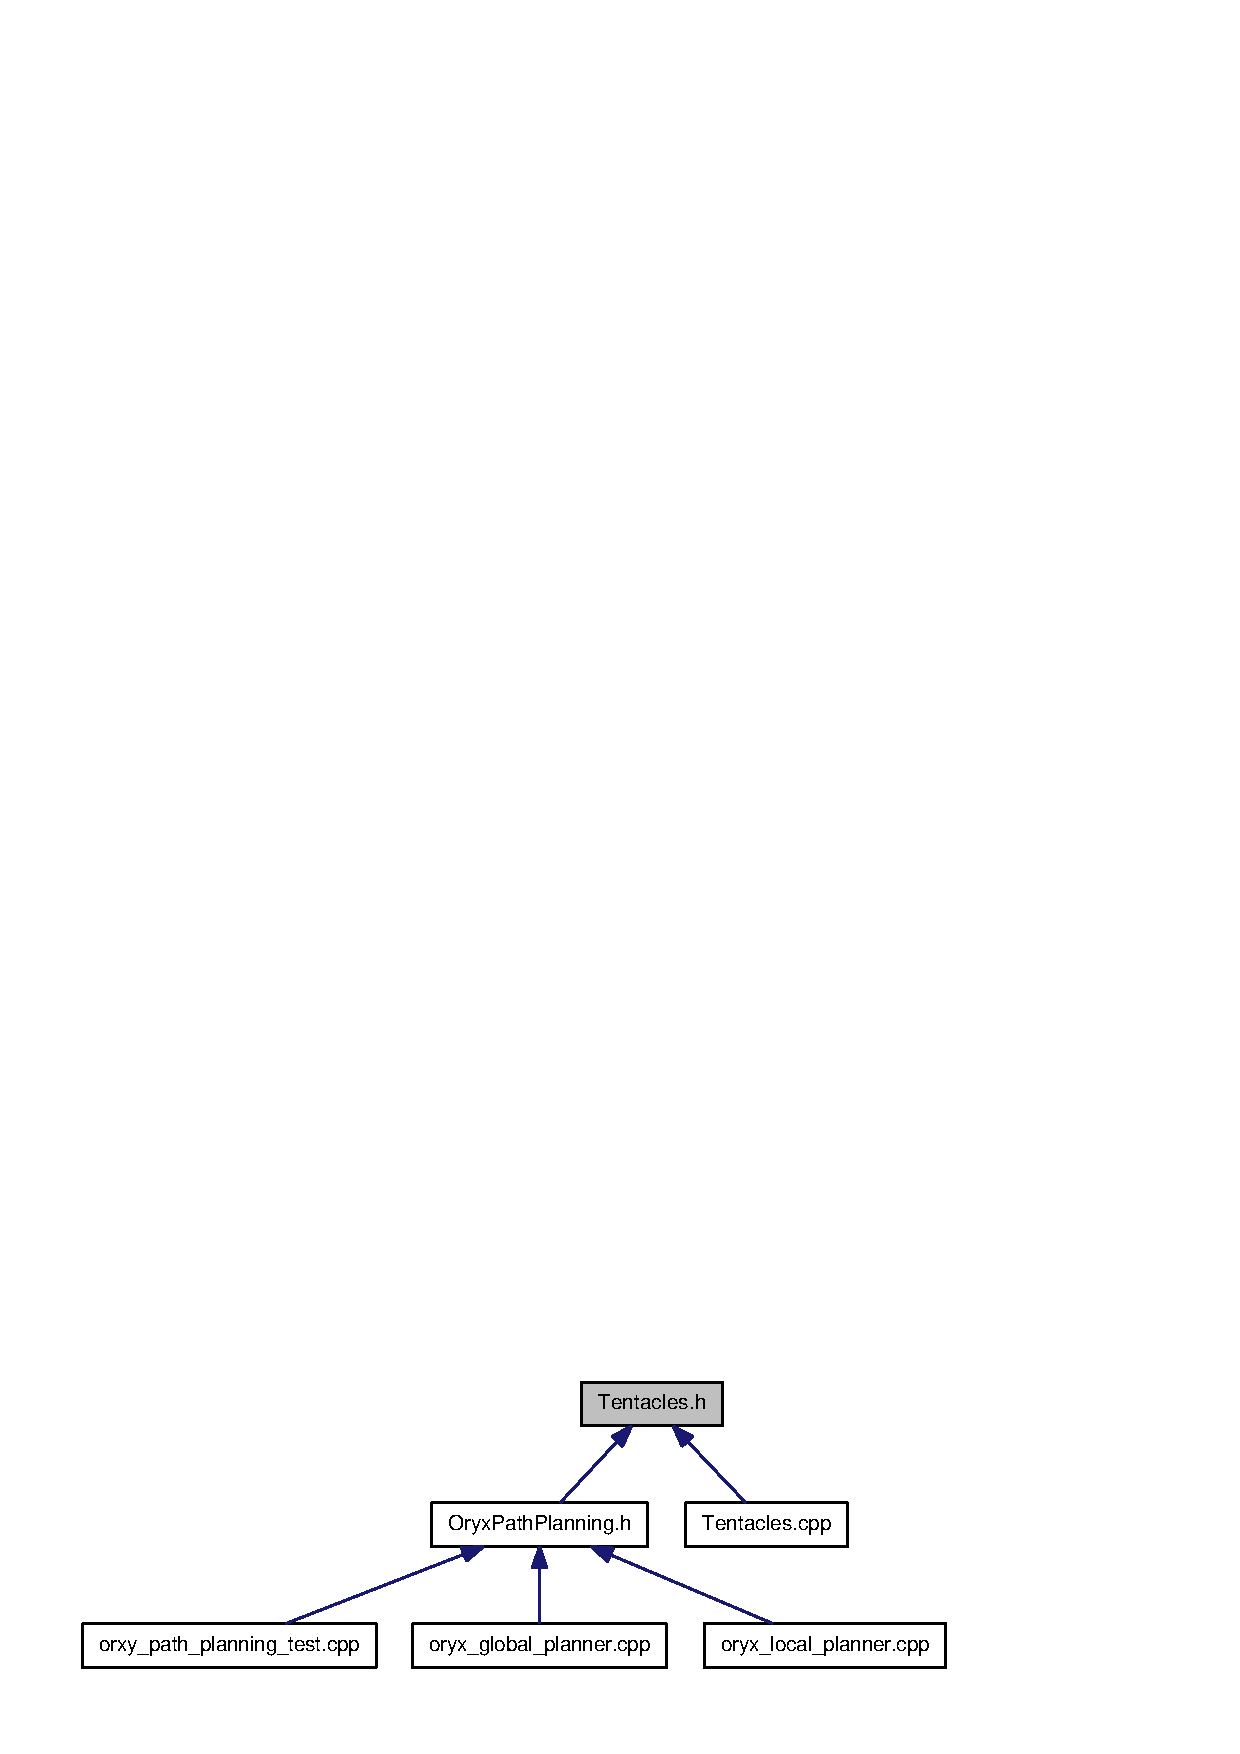
\includegraphics[width=350pt]{Tentacles_8h__dep__incl}
\end{center}
\end{figure}
\subsection*{\-Classes}
\begin{DoxyCompactItemize}
\item 
class {\bf oryx\-\_\-path\-\_\-planning\-::\-Speed\-Set}
\begin{DoxyCompactList}\small\item\em \-Container class for holding tentacle data for a speed set. \end{DoxyCompactList}\item 
class {\bf oryx\-\_\-path\-\_\-planning\-::\-Speed\-Set\-Access\-Exception}
\begin{DoxyCompactList}\small\item\em \-Simple accessor exception that provides some debugging details. \end{DoxyCompactList}\item 
class {\bf oryx\-\_\-path\-\_\-planning\-::\-Tentacle}
\begin{DoxyCompactList}\small\item\em \-Container class for holding data about a tentacle. \end{DoxyCompactList}\item 
class {\bf oryx\-\_\-path\-\_\-planning\-::\-Tentacle\-Access\-Exception}
\begin{DoxyCompactList}\small\item\em \-Simple accessor exception that provides some debugging details. \end{DoxyCompactList}\item 
class {\bf oryx\-\_\-path\-\_\-planning\-::\-Tentacle\-Generation\-Exception}
\begin{DoxyCompactList}\small\item\em \-Exception to flag when there has been a problem generating a tentacle. \end{DoxyCompactList}\item 
class {\bf oryx\-\_\-path\-\_\-planning\-::\-Tentacle\-Generator}
\begin{DoxyCompactList}\small\item\em \-Generates and manages tentacle data. \end{DoxyCompactList}\item 
class {\bf oryx\-\_\-path\-\_\-planning\-::\-Tentacle\-::\-Tentacle\-Traverser}
\begin{DoxyCompactList}\small\item\em \-Helper class for traversing an \doxyref{oryx\-\_\-path\-\_\-planning\-::\-Tentacle}{p.}{classoryx__path__planning_1_1Tentacle}. \end{DoxyCompactList}\end{DoxyCompactItemize}
\subsection*{\-Namespaces}
\begin{DoxyCompactItemize}
\item 
namespace {\bf oryx\-\_\-path\-\_\-planning}
\begin{DoxyCompactList}\small\item\em \-Namespace declaration to make implementation of \-Tentacle\-Traverser easier. \end{DoxyCompactList}\end{DoxyCompactItemize}
\subsection*{\-Typedefs}
\begin{DoxyCompactItemize}
\item 
typedef boost\-::shared\-\_\-ptr\*
$<$ \-Speed\-Set $>$ {\bf oryx\-\_\-path\-\_\-planning\-::\-Speed\-Set\-Ptr}
\begin{DoxyCompactList}\small\item\em \-Typedef to allow for convenient sharing of a \doxyref{\-Speed\-Set}{p.}{classoryx__path__planning_1_1SpeedSet} via shared pointer. \end{DoxyCompactList}\item 
typedef boost\-::shared\-\_\-ptr\*
$<$ \-Tentacle\-Generator $>$ {\bf oryx\-\_\-path\-\_\-planning\-::\-Tentacle\-Generator\-Ptr}
\begin{DoxyCompactList}\small\item\em \-Typedef to allow for convenient sharing of a \doxyref{\-Tentacle\-Generator}{p.}{classoryx__path__planning_1_1TentacleGenerator} via pointer. \end{DoxyCompactList}\item 
typedef boost\-::shared\-\_\-ptr\*
$<$ \-Tentacle $>$ {\bf oryx\-\_\-path\-\_\-planning\-::\-Tentacle\-Ptr}
\begin{DoxyCompactList}\small\item\em \-Typedef to allow for convenient sharing of a \doxyref{\-Tentacle}{p.}{classoryx__path__planning_1_1Tentacle} via shared pointer. \end{DoxyCompactList}\end{DoxyCompactItemize}

\section{\-Type\-Definitions.\-h \-File \-Reference}
\label{TypeDefinitions_8h}\index{\-Type\-Definitions.\-h@{\-Type\-Definitions.\-h}}


\-Common typedefs for the \doxyref{oryx\-\_\-path\-\_\-planning}{p.}{namespaceoryx__path__planning} namespace.  


{\ttfamily \#include $<$pcl/point\-\_\-cloud.\-h$>$}\*
{\ttfamily \#include $<$pcl/point\-\_\-types.\-h$>$}\*
\-Include dependency graph for \-Type\-Definitions.\-h\-:
\nopagebreak
\begin{figure}[H]
\begin{center}
\leavevmode
\includegraphics[width=242pt]{TypeDefinitions_8h__incl}
\end{center}
\end{figure}
\-This graph shows which files directly or indirectly include this file\-:
\nopagebreak
\begin{figure}[H]
\begin{center}
\leavevmode
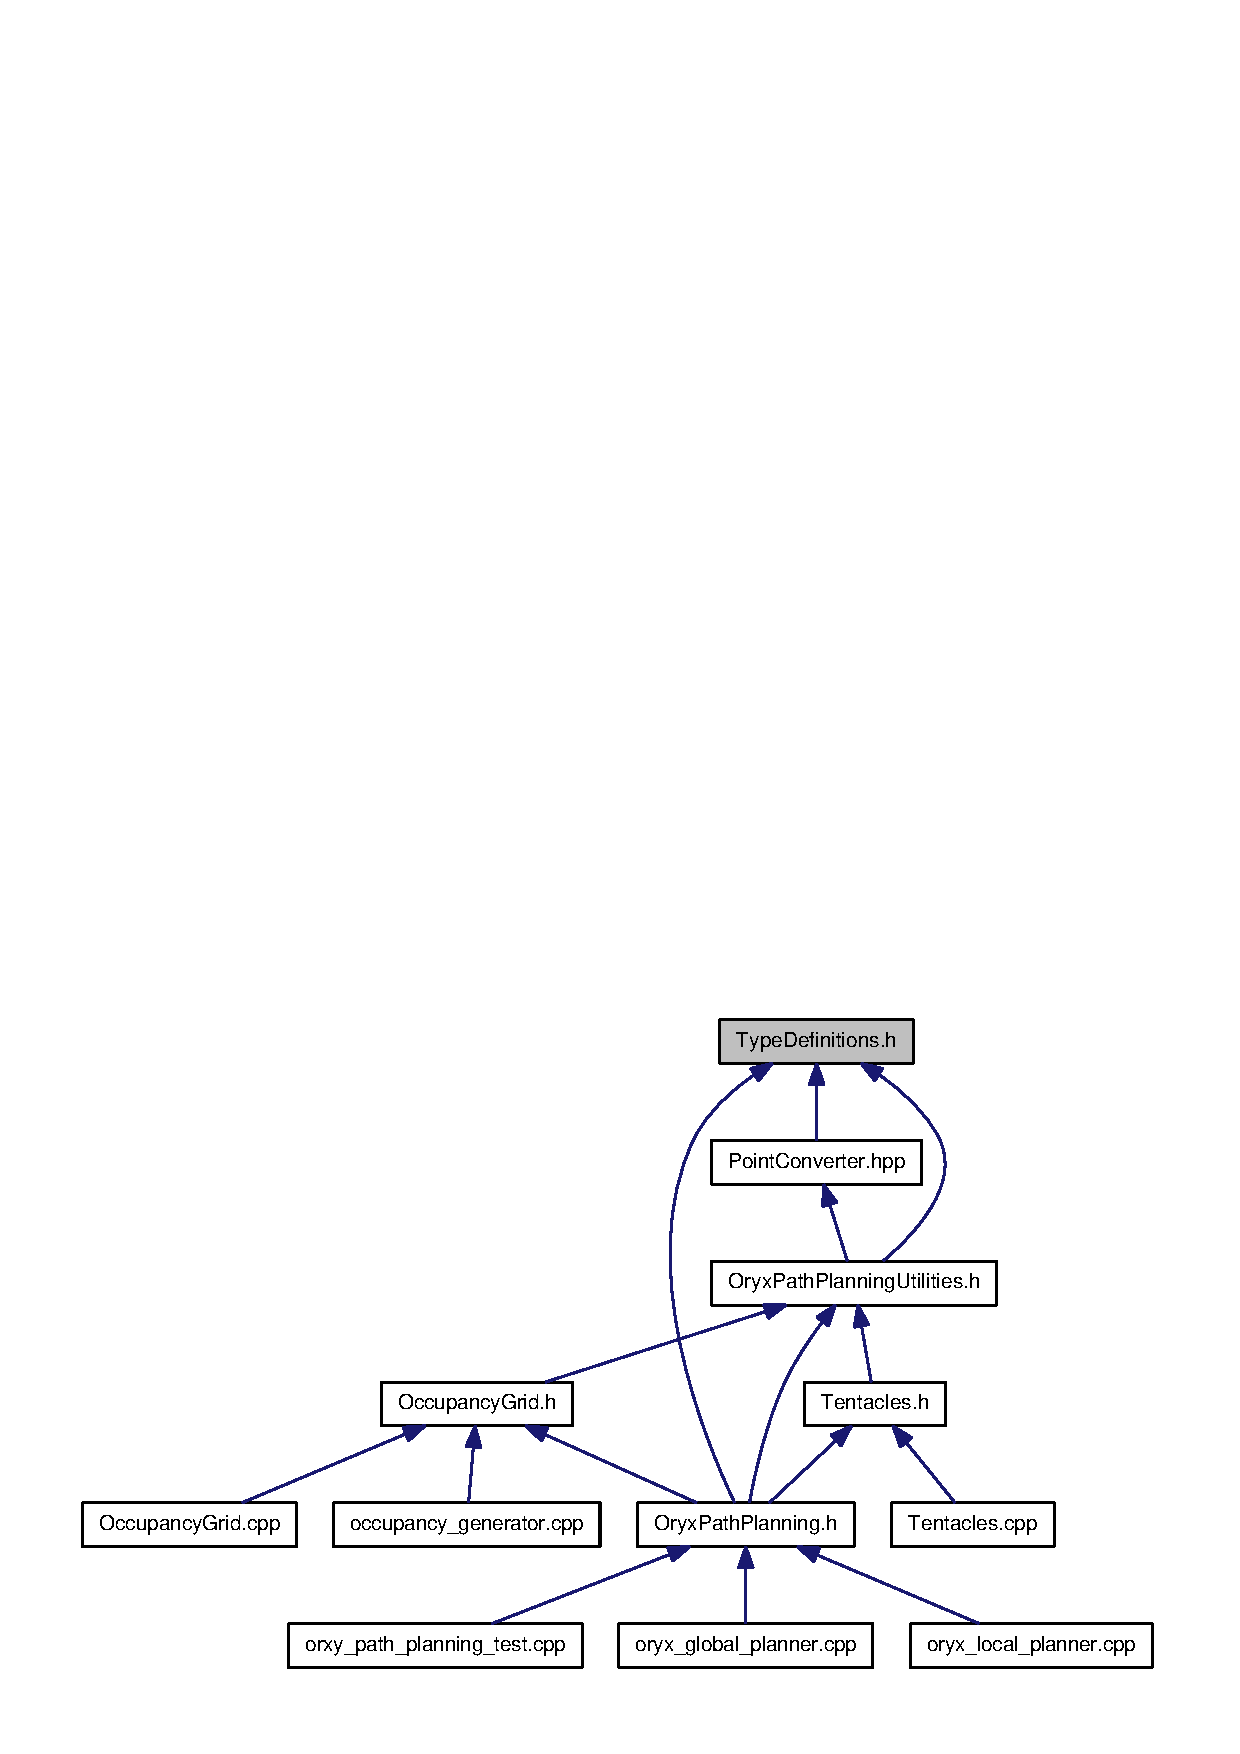
\includegraphics[width=350pt]{TypeDefinitions_8h__dep__incl}
\end{center}
\end{figure}
\subsection*{\-Namespaces}
\begin{DoxyCompactItemize}
\item 
namespace {\bf oryx\-\_\-path\-\_\-planning}
\begin{DoxyCompactList}\small\item\em \-Namespace declaration to make implementation of \-Tentacle\-Traverser easier. \end{DoxyCompactList}\end{DoxyCompactItemize}
\subsection*{\-Typedefs}
\begin{DoxyCompactItemize}
\item 
typedef pcl\-::\-Point\-X\-Y\-Z\-R\-G\-B\-A {\bf oryx\-\_\-path\-\_\-planning\-::\-Point}
\begin{DoxyCompactList}\small\item\em \-Typedef to allow for easier to read code. \end{DoxyCompactList}\item 
typedef pcl\-::\-Point\-Cloud$<$ \-Point $>$ {\bf oryx\-\_\-path\-\_\-planning\-::\-Point\-Cloud}
\begin{DoxyCompactList}\small\item\em \-Typedef to allow for convenient sharing of a \doxyref{\-Point\-Cloud$<$pcl\-::\-Point\-X\-Y\-Z\-R\-G\-B\-A$>$}{p.}{namespaceoryx__path__planning_a5cfb5ee0e8e3fa2f2ca2d7aeabbf2be7} \end{DoxyCompactList}\item 
typedef boost\-::shared\-\_\-ptr\*
$<$ pcl\-::\-Point\-Cloud$<$ \-Point $>$ $>$ {\bf oryx\-\_\-path\-\_\-planning\-::\-Point\-Cloud\-Ptr}
\begin{DoxyCompactList}\small\item\em \-Typedef to allow for convenient sharing of a \doxyref{\-Point\-Cloud$<$pcl\-::\-Point\-X\-Y\-Z\-R\-G\-B\-A$>$}{p.}{namespaceoryx__path__planning_a5cfb5ee0e8e3fa2f2ca2d7aeabbf2be7} $>$ via pointer. \end{DoxyCompactList}\item 
typedef boost\-::shared\-\_\-ptr$<$ \-Point $>$ {\bf oryx\-\_\-path\-\_\-planning\-::\-Point\-Ptr}
\begin{DoxyCompactList}\small\item\em \-Typedef to allow for convenient sharing of a pcl\-::\-Point\-X\-Y\-Z\-R\-G\-B\-A via pointer. \end{DoxyCompactList}\end{DoxyCompactItemize}


\subsection{\-Detailed \-Description}
\-Common typedefs for the \doxyref{oryx\-\_\-path\-\_\-planning}{p.}{namespaceoryx__path__planning} namespace. \begin{DoxyDate}{\-Date}
\-Nov 1, 2012 
\end{DoxyDate}
\begin{DoxyAuthor}{\-Author}
\-Adam \-Panzica 
\end{DoxyAuthor}


\-Definition in file {\bf \-Type\-Definitions.\-h}.


\printindex
\end{document}
